\documentclass[xcolor=dvipsnames,compress,t,pdf,notes,9pt]{beamer}
\usepackage{beamerthemeshadow}
\usepackage{adjustbox}
\usepackage{lmodern}
\usepackage{booktabs}
%\usepackage{enumitem}
\usepackage[english]{babel}
\usepackage{tikz-qtree} 
%\usepackage{listings}
%\usepackage{flashmovie}
\usepackage{media9}
\usepackage{makecell}
 \usepackage{multimedia}
 \usepackage{listings}
 \usepackage{color}
 % \usepackage{helvet}
\definecolor{codegreen}{rgb}{0,0.6,0}
\definecolor{codegray}{rgb}{0.5,0.5,0.5}
\definecolor{codepurple}{rgb}{0.58,0,0.82}
\definecolor{backcolour}{rgb}{.914, .89, .957} % pale purple

\definecolor{mygreen}{rgb}{0,0.6,0}
\definecolor{mygray}{rgb}{0.5,0.5,0.5}
\definecolor{mymauve}{rgb}{0.58,0,0.82}

\lstdefinestyle{mystyle}{
  backgroundcolor=\color{backcolour},   % choose the background color; you must add \usepackage{color} or \usepackage{xcolor}; should come as last argument
  basicstyle=\footnotesize\ttfamily,       % the size of the fonts that are used for the code
  breakatwhitespace=true,          % sets if automatic breaks should only happen at whitespace
  breaklines=true,                 % sets automatic line breaking
  captionpos=b,                    % sets the caption-position to bottom
  commentstyle=\color{mygreen},    % comment style
  deletekeywords={...},            % if you want to delete keywords from the given language
  escapeinside={\%*}{*)},          % if you want to add LaTeX within your code
  extendedchars=true,              % lets you use non-ASCII characters; for 8-bits encodings only, does not work with UTF-8
  frame=single,	                   % adds a frame around the code
  keepspaces=true,                 % keeps spaces in text, useful for keeping indentation of code (possibly needs columns=flexible)
  keywordstyle=\color{blue},       % keyword style
  language=Python,                 % the language of the code
  morekeywords={*,...},            % if you want to add more keywords to the set
  numbers=left,                    % where to put the line-numbers; possible values are (none, left, right)
  numbersep=5pt,                   % how far the line-numbers are from the code
  numberstyle=\tiny\color{mygray}, % the style that is used for the line-numbers
  rulecolor=\color{black},         % if not set, the frame-color may be changed on line-breaks within not-black text (e.g. comments (green here))
  showspaces=false,                % show spaces everywhere adding particular underscores; it overrides 'showstringspaces'
  showstringspaces=false,          % underline spaces within strings only
  showtabs=false,                  % show tabs within strings adding particular underscores
  stepnumber=2,                    % the step between two line-numbers. If it's 1, each line will be numbered
  stringstyle=\color{mymauve},     % string literal style
  tabsize=2,	                   % sets default tabsize to 2 spaces
  columns=fullflexible,
  linewidth=0.98\linewidth,        % Box width
  aboveskip=10pt,	   			   % Space before listing 
  belowskip=-15pt,	   			   % Space after listing  
  xleftmargin=.02\linewidth,  
  title=\lstname                   % show the filename of files included with \lstinputlisting; also try caption instead of title
}


% \definecolor{codegreen}{rgb}{0,0.6,0}
% \definecolor{codegray}{rgb}{0.5,0.5,0.5}
% \definecolor{codepurple}{rgb}{0.58,0,0.82}
% %\definecolor{backcolour}{rgb}{0.95,0.95,0.92} % faint postman color
% \definecolor{backcolour}{rgb}{.914, .89, .957} % pale purple
% %\lstset{basicstyle=\footnotesize\ttfamily}

% \lstdefinestyle{mystyle}{
    % backgroundcolor=\color{backcolour},   
    % commentstyle=\color{codegreen},
    % keywordstyle=\color{magenta},
    % numberstyle=\tiny\color{codegray},
    % stringstyle=\color{codepurple},
    % basicstyle= \tiny\ttfamily %\scriptsize\ttfamily, %\footnotesize,  % the size of the fonts that are used for the code
    % breakatwhitespace=true,  % sets if automatic breaks should only happen at whitespace        
    % breaklines=true, % sets automatic line breaking   
    % linewidth=\linewidth,	
    % captionpos=b,                    
    % keepspaces=true,% keeps spaces in text, useful for keeping indentation                
% %    numbers=left,                  
    % numbers=none,  
% %    numbersep=5pt,                  
    % showspaces=false,                
    % showstringspaces=false,
    % showtabs=false,                  
    % tabsize=2
% }
\lstset{style=mystyle}

\usetheme{Warsaw}
\usecolortheme{whale}
\usefonttheme{structuresmallcapsserif}
\useinnertheme{rounded}
\useoutertheme[subsection=false,footline=authortitle]{miniframes}   

\setbeamerfont{block title}{size={}}

\definecolor{darkpurple}{rgb}{0.471,0.008,0.412}
\definecolor{middlepurple}{rgb}{0.663,0.012,0.580}
\definecolor{lightpurple}{rgb}{0.855,0.016,0.749}
\definecolor{gold}{RGB}{254,232,0}
\definecolor{nyupurple}{RGB}{90, 35, 140}
\definecolor{lightnyupurple}{RGB}{159, 120, 184}

\setbeamercolor{alerted text}{fg=nyupurple}
\setbeamercolor{example text}{fg=darkgray}

\setbeamercolor*{palette secondary}{fg=white,bg=lightnyupurple} %subsection
\setbeamercolor*{palette tertiary}{fg=white,bg=nyupurple} %section

\setbeamercolor{title}{fg=black, bg=lightnyupurple}         %Title of presentation
\setbeamercolor{block title}{fg=white, bg=nyupurple}
\setbeamercolor{section title}{fg=white, bg=nyupurple}
\setbeamercolor{subsection title}{fg=white, bg=lightnyupurple}
%\setbeamercolor{frametitle}{fg=white, bg=lightnyupurple}  % Gives gradient in the frame title bar
\setbeamertemplate{frametitle}[default][colsep=-4bp,rounded=false,shadow=false] % disable gradient

\setbeamerfont{frametitle}{size=\large}
\setbeamerfont{frametitle}{series=\bfseries}

\setbeamertemplate{blocks}[rounded][shadow=true] 
\setbeamertemplate{items}[triangle]
\setbeamercolor{item}{fg=gray, bg=white}

\setbeamertemplate{navigation symbols}{}
\setbeamertemplate{bibliography entry title}{}
\setbeamertemplate{bibliography entry location}{}
\setbeamertemplate{bibliography entry note}{}
\setbeamertemplate{bibliography item}{}

\beamertemplatenavigationsymbolsempty
\setbeamercovered{transparent}

\setbeamertemplate{itemize item}{\scriptsize\raise1.25pt\hbox{\donotcoloroutermaths$\blacktriangleright$}}
\setbeamertemplate{itemize subitem}{\tiny\raise1.5pt\hbox{\donotcoloroutermaths$\blacktriangleright$}}
\setbeamertemplate{itemize subsubitem}{\tiny\raise1.5pt\hbox{\donotcoloroutermaths$\blacktriangleright$}}
\setbeamertemplate{enumerate item}{\insertenumlabel.}
\setbeamertemplate{enumerate subitem}{\insertenumlabel.\insertsubenumlabel}
\setbeamertemplate{enumerate subsubitem}{\insertenumlabel.\insertsubenumlabel.\insertsubsubenumlabel}
\setbeamertemplate{enumerate mini template}{\insertenumlabel}
\setbeamertemplate{mini frames}{}
%\setbeamertemplate{itemize/enumerate subbody begin}{\vspace{1cm}}
%\setbeamertemplate{itemize/enumerate subbody end}{\vspace{1cm}}

% TOC at start of a Section or a Subsection
\AtBeginSection[] { 
  \begin{frame}[plain] 
    \frametitle{Agenda} 
    \tableofcontents[currentsection] 
  \end{frame} 
  \addtocounter{framenumber}{-1} 
} 

%\AtBeginSubsection[] { 
%  \begin{frame}[plain] 
%   \frametitle{Agenda} 
%    \tableofcontents[currentsubsection] 
%    \addtocounter{framenumber}{-1} 
%  \end{frame} 
%} 


%\logo{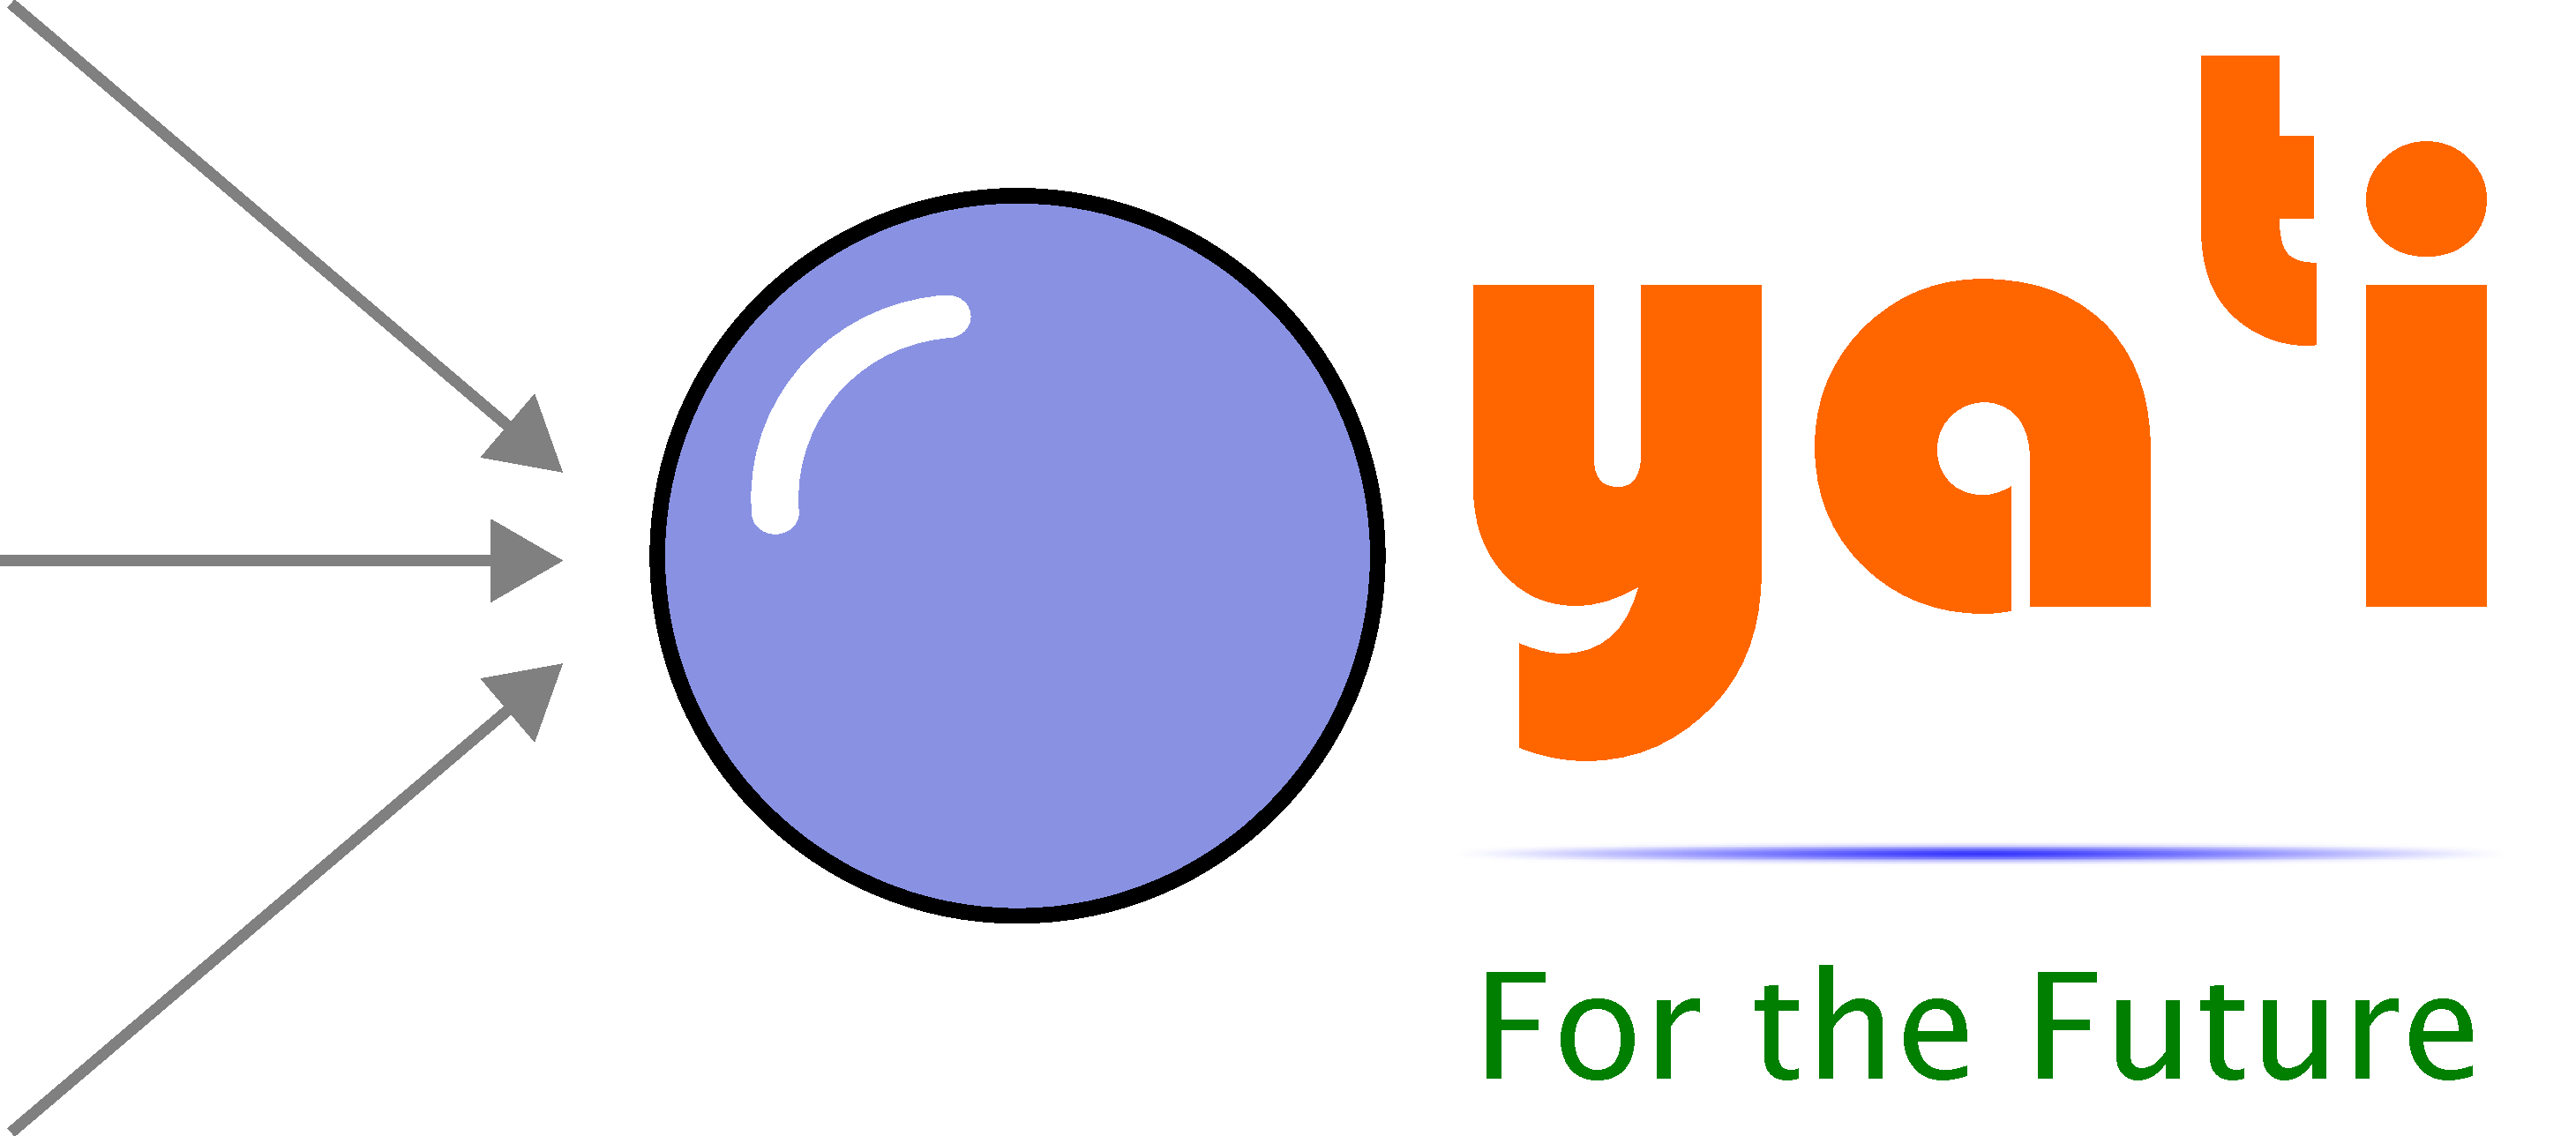
\includegraphics[width=2cm,keepaspectratio]{images/yati_logo.pdf}}
\author[Yogesh H Kulkarni]{Yogesh Kulkarni} 

\newcommand{\code}[1]{\par\vskip0pt plus 1filll \footnotesize Code:~\itshape#1}

\setbeameroption{hide notes}
\graphicspath{{./images/}}
% 
\newtheorem{axiom}{Axiom}[theorem]
%\newtheorem{conj}{Conjecture}[theorem]


%%%%
%%%% colors
%%%%
\newcommand{\TealBlue}[1]{\textcolor{TealBlue}{#1}}
\newcommand{\Peach}[1]{\textcolor{Peach}{#1}}
\newcommand{\Cyan}[1]{\textcolor{cyan}{#1}}
\newcommand{\Red}[1]{\textcolor{red}{#1}}
\newcommand{\BrickRed}[1]{\textcolor{BrickRed}{#1}}
\newcommand{\Blue}[1]{\textcolor{blue}{#1}}
\newcommand{\Green}[1]{\textcolor{green}{#1}}
\newcommand{\Black}[1]{\textcolor{black}{#1}}
\newcommand{\White}[1]{\textcolor{white}{#1}}
\newcommand{\Blueit}[1]{\textcolor{Blue}{\emph{#1}}}
\newcommand{\Magentait}[1]{\textcolor{Magenta}{\emph{#1}}}
\newcommand{\Orangeit}[1]{\textcolor{Orange}{\emph{#1}}}
\newcommand{\Greenit}[1]{\textcolor{Green}{\emph{#1}}}
\newcommand{\Cyanit}[1]{\textcolor{cyan}{\emph{#1}}}


%
%  Macros
%

\newcommand{\RingNat}{{{\mathbb{N}}}}
\newcommand{\RingInt}{{{\mathbb{Z}}}}
\newcommand{\RingReal}{{{\mathbb{R}}}}
\newcommand{\RingRat}{{{\mathbb{Q}}}}
\newcommand{\RingPosInt}{{{\mathbb{Z^+}}}}
\newcommand{\myand}{\wedge}
\newcommand{\myor}{\vee}
\newcommand{\mynot}{\neg}

% \newcommand{\pict}[3]{\resizebox{#1in}{#2in}{\includegraphics{#3}}}
\newcommand{\pictt}[1]{\includegraphics{#1}}
\newcommand{\Frac}[2]{\frac{\textstyle #1}{\textstyle #2}}

\newcommand{\der}{\operatorname{Der}} 
\newcommand{\embdim}{\operatorname{emb. dim.}} 
\newcommand{\support}{\operatorname{Support}} 
\newcommand{\coker}{\operatorname{coker}} 
\newcommand{\nind}{\noindent}
\newcommand{\Z}{\mathfrak{Z}} 
\newcommand{\E}{\mathcal{E}} 
\newcommand{\disp}{\displaystyle}

\def\bbd#1{\leavevmode\setbox0=\hbox{#1}%
   	\kern-.025em\copy0 \kern-\wd0
   	\kern .05em\copy0 \kern-\wd0
  	\kern-.025em\raise.0433em\box0
  	}
   	\def\nexto{\kern -0.54em}
    	\def\DN{ \mbox{\rm {I\ \nexto N}} }
    	\def\DZ{ \mbox{\rm Z \kern -0.82em Z} }
    	\def\DC{ \mbox{\rm\hbox{C \kern-0.8em\raise0.2ex
    	\hbox{\vrule height5.4pt width0.7pt} \kern0.45em}} }
    	\def\DQ{ \mbox{\rm\hbox{Q \kern-0.85em\raise0.25ex
    	\hbox{\vrule height5.4pt width0.7pt} \kern0.45em}} }
    	\def\DP{ \mbox{\rm\hbox{P\kern-0.75em	
    	\hbox{\vrule height9pt width0.7pt} \kern0.45em}} }
\newcommand{\bigfrac}[2]{\frac{\textstyle #1}{\textstyle #2}}
 \newcommand{\starttest}{\begin{enumerate}}
 \newcommand{\nextpage}{\vspace*{\fill}\newpage}

 \newcommand{\mat}[2]{\left( \begin{array}{*{#1}{c}}#2\end{array}\right)}
 \newcommand{\matr}[2]{\left( \begin{array}{*{#1}{r}}#2\end{array}\right)}
 
 \newcommand{\bmat}[2]{\left[ \begin{array}{*{#1}{c}}#2\end{array}\right]}
 \newcommand{\bmatr}[2]{\left[ \begin{array}{*{#1}{r}}#2\end{array}\right]}
 
 \newcommand{\dat}[2]{\left| \begin{array}{*{#1}{c}}#2\end{array}\right|}
 \newcommand{\datr}[2]{\left| \begin{array}{*{#1}{r}}#2\end{array}\right|}
 \newcommand{\deff}[1]{\vspace*{0.2in} {\bf Definition: #1}}
 \newcommand{\lineend}{\vspace*{0.1in}\centerline{\rule{4in}{0.01in}}}

 \newcommand{\seg}[1]{\overline{#1}}
 \newcommand{\ray}[1]{\overrightarrow{#1}}
 \newcommand{\lin}[1]{\overleftrightarrow{#1}}
 \newcommand{\sdash}{\!\!-\!\!}
 \newcommand{\betw}[3]{#1\sdash#2\sdash#3}
   \newcommand{\bs}{$\backslash$}

 \newcommand{\mrd}[1]{\textcolor{red}{#1}}%% Make entry red
 \newcommand{\mbl}[1]{\textcolor{blue}{#1}}%% Make entry blue
 
 \newcommand{\mgr}[1]{\textcolor{green!40!black}{#1}}%% Make entry green

\newcommand{\mbr}[1]{\textcolor{blue!55!red}{#1}}%% Make entry purple


\newtheorem{thm}{Theorem}[section]
%\newtheorem{Conjecture}[thm]{Conjecture}
%\newtheorem{Lemma}[thm]{Lemma}
%\newtheorem{corollary}[thm]{Corollary}
%\newtheorem{proposition}[thm]{Proposition} 
\newtheorem{question}[thm]{Question} 

\newtheorem*{defn}{Definition}

% \newcommand{\ignore}[1]{}
\newcommand{\arcosh}{\qopname \relax o{arcosh}}
\newcommand{\divop}{\qopname \relax o{div}}
\newcommand{\dist}{\qopname \relax o{dist}}
\newcommand{\D}{\qopname \relax o{D}\!} 	% Jacobi-Matrix
\newcommand{\dop}{\qopname \relax o{d}\!} 	% Differentialoperator
\newcommand{\ds}{\dop s}
\newcommand{\dt}{\dop t}
\newcommand{\dx}{\dop x}
\newcommand{\dy}{\dop y}
\newcommand{\Epi}{\qopname \relax o{Epi}}
\newcommand{\hot}{\qopname \relax o{hot}}
\newcommand{\id}{\qopname \relax o{id}}
\newcommand{\im}{\qopname \relax o{im}}
\newcommand{\osc}{\qopname \relax o{osc}}
%\newcommand{\rg}{\qopname \relax o{rg}}
\newcommand{\rot}{\qopname \relax o{rot}}
%\newcommand{\Satz}{Proposition }
\newcommand{\SatzEnde}{r}
\newcommand{\sgn}{\qopname \relax o{sgn}}
\newcommand{\tr}{\qopname \relax o{tr}}
\hyphenation{Hil-bert-raum}
%adrian
\newcommand{\Norm}[1]{\left\| #1 \right\|}
\newcommand{\SKP}[1]{\left\langle #1 \right\rangle}

%\newcommand\mat[2][c]{\left(\hspace{-2mm}\begin{array}{#1}#2\end{array}\hspace{-2mm}\right)}

% praktische Extras:
% Liste mit a), b) etc. vor den Items (alphanumerisch)
% zuerst der Anfang
\newcommand{\bal}[1]{\newcounter{#1}\stepcounter{#1}\begin{list}{\alph{#1})}{}}
  % jetzt die einzelnen items
  \newcommand{\aitem}[1]{\item\stepcounter{#1}}
  % zuletzt das Ende
  \newcommand{\eal}{\end{list}}
% Liste mit i), ii) etc. vor den Items (roman)
% Anfang
\newcommand{\brl}[1]{\newcounter{#1}\stepcounter{#1}\begin{list}{\roman{#1})}{}}
  % item
  \newcommand{\ritem}[1]{\item\stepcounter{#1}}
  % Ende
  \newcommand{\erl}{\end{list}}
% Matrix-Anfang und -Ende
% Anfang
\newcommand{\matb}[1]{\left(\begin{array}{#1}}
    % Ende
    \newcommand{\mate}{\end{array}\right)}
% Vektor-Anfang und -Ende
% Anfang
\newcommand{\vekb}{\left(\begin{array}{c}}
    % Ende
    \newcommand{\veke}{\end{array}\right)}
% Die Standardk�rper Q,R,C,F,N,Z
% Q
\newcommand{\Ku}{\mathbb{Q}}
% R
\newcommand{\Er}{\mathbb{R}}
% C
\newcommand{\Ze}{\mathbb{C}}
% F
\newcommand{\Ef}{\mathbb{F}}
% N
\newcommand{\En}{\mathbb{N}}
% Z
\newcommand{\Zett}{\mathbb{Z}}
% eqnarray
% Anfang
\newcommand{\bea}{\begin{eqnarray*}}
% Ende
\newcommand{\eea}{\end{eqnarray*}}
% Theoreme, S�tze, Beispiele etc.
\theoremstyle{plain}
%\newtheorem{theorem}{Theorem}[section]
%\newtheorem{korollar}[theorem]{Korollar}
%\newtheorem{lemma}[theorem]{Lemma}
\newtheorem{proposition}[theorem]{\Satz}
%\newtheorem{conjecture}[theorem]{Vermutung}
%\newtheorem{satz}[theorem]{\Satz}
%\theoremstyle{definition}
%\newtheorem{definition}[theorem]{Definition}
%%\theoremstyle{remark}
%\newtheorem{notation}[theorem]{Notation}
%\newtheorem{remark}[theorem]{Remark}
%\newtheorem{corollary}[theorem]{Corollary}
%\newtheorem{application}[theorem]{Application}
%\newtheorem{example}[theorem]{Example}
%\newtheorem*{remark*}{Bemerkung}
%\newtheorem*{example*}{Example}
%\newtheorem*{notation*}{Bezeichnung}
%\newtheorem*{application*}{Anwendung}

%\newenvironment{proof}[1][Beweis]{\begin{trivlist}
%  \item[\hskip \labelsep {\bfseries #1}]}{\end{trivlist}}
% \newenvironment{definition}[1][Definition]{\begin{trivlist}
% \item[\hskip \labelsep {\bfseries #1}]}{\end{trivlist}}
%\newenvironment{example}[1][Example]{\begin{trivlist}
%  \item[\hskip \labelsep {\bfseries #1}]}{\end{trivlist}}
%\newenvironment{remark}[1][Remark]{\begin{trivlist}
%  \item[\hskip \labelsep {\bfseries #1}]}{\end{trivlist}}

% Beginn Symboldef Mitterlwertintegral-----------------------------------
\def \Xint #1{\mathchoice						
  {\XXint \displaystyle \textstyle {#1}} %
  {\XXint \textstyle \scriptstyle {#1}} %
  {\XXint \scriptstyle \scriptscriptstyle {#1}} %
  {\XXint \scriptscriptstyle \scriptscriptstyle {#1}} %
  \!\int }

\def \XXint #1#2#3{{\setbox 0=\hbox {$#1{#2#3}{\int }$}\vcenter {\hbox {$#2#3$}}\kern -0.5\wd 0}}

\def \dashint {\Xint -}							

% Fallunterscheidung
\newcommand {\Fall}[5]
    { #1 = \left \{
        \begin{array}
         {c@ {\quad \mbox{ if } \quad} l}
          #2 & #3 \\
           #4 & #5           \end{array}
            \right .    }


\newcommand {\Falldrei}[7]
       { #1 = \left \{
          \begin{array}
             {c@ {\quad \mbox{ if } \quad} l}
               #2 & #3 \\
            #4 & #5 \\ 														             \right .    }



% \renewcommand{\P}{\text{P}}
%\newcommand{\R}{{\rm I\!R}}
\newcommand{\pr}{{\rm I\!P}}
%%%\newcommand{\E}{{\rm I\!E}}
\newcommand{\Na}{{\rm I\!N}}
\newtheorem{conj}{Conjecture}
\newtheorem{countex}{Counterexample}
\newtheorem{prop}{Proposition}
%%%\newtheorem{thm}{Theorem}
\newtheorem{cor}{Corollary}
%%%\newtheorem{defn}{Definition}
\newtheorem{lem}{Lemma}
%\renewcommand{\ell}{l}
\newcommand{\SSS}{\scriptscriptstyle}
\newcommand{\MC}{\multicolumn}
\newcommand{\cT}{\ensuremath{{\cal T}}}
\newcommand{\z}{\ensuremath{\pi}}
\newcommand{\sZ}{\ensuremath{\Pi}}
\newcommand{\bz}{\ensuremath{\mbox{\boldmath$\pi$}}}
\newcommand{\Pperm}{\ensuremath{{\hat{P}}}}
\newcommand{\Pnull}{\ensuremath{{{P}_{\mbox{null}}}}}
\newcommand{\bx}{\ensuremath{{\bf x}}}
\newcommand{\bzz}{\ensuremath{{\bf z}}}
\def\ssucc{{\succ\!\!\!\!\succ}}
%\DeclareMathOperator\Tr{Tr}
% set up hyperlink colors
\hypersetup{colorlinks=true,anchorcolor=green,linkcolor=red,menucolor=cyan}
%%================Math symbol ============================
\def\nn{{\mathbb N}}
\def\zz{{\mathbb Z}}
\def\rr{{\mathbb R}}
\def\rn{{\mathbb R}^n}
\def\ym{Y^{m}}\def\xm{X^{m}}
\def\yp{Y^{p}}\def\xp{X^{p}}
\def\yr{Y^{r}}\def\xr{X^{r}}
\def\yj{Y^{j}}\def\xj{X^{j}}

\def\yij#1#2{y_{#2}^{#1}}\def\xij#1#2{x_{#2}^{#1}}


%%=============Display style operator =====================
\def\dsum{\displaystyle\sum}
\def\dint{\displaystyle\int}
\def\dfrac{\displaystyle\frac}
\def\dsup{\displaystyle\sup}
\def\dinf{\displaystyle\inf}
\def\dmin{\displaystyle\min}
\def\dlim{\displaystyle\lim}


%%=========Greek Letters =================
\def\gep{\varepsilon}
\def\ga{\alpha}
\def\gb{\beta}
\def\gs{\sigma}
\def\gd{\delta}
\def\gl{\lambda}
\def\gga{\gamma}
\def\gS{\Sigma}
\def\gD{\Delta}
\def\px{{\rho\!_{_X}}}
\def\L{{\cal L}} %
\def\B{{\cal B}} %
\def\X{{\cal X}} %
\def\M{{\cal M}} %

%============ Special notations ===============
\newcommand{\set}[1]{\left\{#1\right\}} % set
\def\E{{\mathcal E}} % generalization error
\def\H{{\mathcal H}} % hypothesis space
\def\H{{\mathcal H}} % hypothesis space
\def\N{{\mathcal N}} % covering number
\def\D{{\mathcal D}} % regularization error
\def\bz{{\bf z}} % sample
%%%\DeclareMathOperator\sgn{sgn} % sign function
\DeclareMathOperator\Span{span} % linear span
\DeclareMathOperator\Diam{Diam} % diameter of a set
\DeclareMathOperator\bE{\mathbb E} % expectation
\DeclareMathOperator*\prob{{\bf P}rob} % probability in product space


% %\makeatletter
\DeclareRobustCommand*{\savepause}[1]{\only<1>{\immediate\write\@auxout{\string\pauseentry{\the\c@framenumber}{#1}{\the\c@beamerpauses}}}}
\newcommand*{\usepause}[1]{\@ifundefined{pauses@\the\c@framenumber @#1}{1}{\@nameuse{pauses@\the\c@framenumber @#1}}}
\newcommand*{\pauseentry}[3]{\global\@namedef{pauses@#1@#2}{#3}}

\makeatother\newcommand{\floor}[1]{\lfloor{#1}\rfloor}

\setbeamertemplate{navigation symbols}{}
\tikzset{
vertex/.style={circle,draw=blue!50,thick},
}
\tikzset{
vertex/.style={circle,draw=blue!50,thick},
}

\tikzset{
bluedot/.style={circle,draw=blue,fill=blue,thick},
}

\tikzset{
littlevertx/.style={minimum width=1pt,minimum width=1pt,text width=1pt},
}



\tikzset{
dot/.style={circle,draw=black,thick},
}

\tikzset{
reddot/.style={circle,draw=red,fill=red,thick},
}

\tikzset{
orangedot/.style={circle,draw=orange,fill=orange ,thick},
}

\tikzset{
packet/.style={rectangle,draw=black,fill=white,thick},
}

\tikzset{
lostpacket/.style={rectangle,draw=red,fill=red,thick},
}

\tikzset{
corruptpacket/.style={rectangle,draw=red,thick},
}

\tikzset{
greendot/.style={circle,draw=green,fill=green,thick},
}

\tikzset{
entity/.style={rectangle,draw=blue!50,thick},
}
\newcommand{\bl}[2]{{\color<#1>{blue} #2}}
\renewcommand{\gl}[2]{{\color<#1>{green} #2}}
\newcommand{\rl}[2]{{\color<#1>{red} #2}}
\newcommand{\orl}[2]{{\color<#1>{orange} #2}}
\newcommand{\ol}[2]{{\onslide<#1>{#2}}}
\newcommand{\xor}{\oplus}

\newcommand{\spd}[1]{#1 {\color{black} \spadesuit}}
\newcommand{\clb}[1]{#1 {\color{black} \clubsuit}}
\newcommand{\dmd}[1]{#1 {\color{red} \diamondsuit}}
\newcommand{\hrt}[1]{#1 {\color{red} \heartsuit}}

\newcommand{\hl}[1]{{\color{blue}#1}}
\newcommand{\orli}[1]{{\color{orange}#1}}
%\usepackage{pstricks, pst-node}

%
%	THE GRID - UNLABELED VERTICES
%
\newcommand{\Gaa}{\put(0,0){\circle*{3}}}
\newcommand{\Gba}{\put(10,0){\circle*{3}}}
\newcommand{\Gca}{\put(20,0){\circle*{3}}}
\newcommand{\Gda}{\put(30,0){\circle*{3}}}
\newcommand{\Gea}{\put(40,0){\circle*{3}}}
\newcommand{\Gfa}{\put(50,0){\circle*{3}}}
\newcommand{\Gga}{\put(60,0){\circle*{3}}}

\newcommand{\Gab}{\put(0,10){\circle*{3}}}
\newcommand{\Gbb}{\put(10,10){\circle*{3}}}
\newcommand{\Gcb}{\put(20,10){\circle*{3}}}
\newcommand{\Gdb}{\put(30,10){\circle*{3}}}
\newcommand{\Geb}{\put(40,10){\circle*{3}}}
\newcommand{\Gfb}{\put(50,10){\circle*{3}}}
\newcommand{\Ggb}{\put(60,10){\circle*{3}}}

\newcommand{\Gac}{\put(0,20){\circle*{3}}}
\newcommand{\Gbc}{\put(10,20){\circle*{3}}}
\newcommand{\Gcc}{\put(20,20){\circle*{3}}}
\newcommand{\Gdc}{\put(30,20){\circle*{3}}}
\newcommand{\Gec}{\put(40,20){\circle*{3}}}
\newcommand{\Gfc}{\put(50,20){\circle*{3}}}
\newcommand{\Ggc}{\put(60,20){\circle*{3}}}

\newcommand{\Gad}{\put(0,30){\circle*{3}}}
\newcommand{\Gbd}{\put(10,30){\circle*{3}}}
\newcommand{\Gcd}{\put(20,30){\circle*{3}}}
\newcommand{\Gdd}{\put(30,30){\circle*{3}}}
\newcommand{\Ged}{\put(40,30){\circle*{3}}}
\newcommand{\Gfd}{\put(50,30){\circle*{3}}}
\newcommand{\Ggd}{\put(60,30){\circle*{3}}}

\newcommand{\Gae}{\put(0,40){\circle*{3}}}
\newcommand{\Gbe}{\put(10,40){\circle*{3}}}
\newcommand{\Gce}{\put(20,40){\circle*{3}}}
\newcommand{\Gde}{\put(30,40){\circle*{3}}}
\newcommand{\Gee}{\put(40,40){\circle*{3}}}
\newcommand{\Gfe}{\put(50,40){\circle*{3}}}
\newcommand{\Gge}{\put(60,40){\circle*{3}}}

\newcommand{\Gaf}{\put(0,50){\circle*{3}}}
\newcommand{\Gbf}{\put(10,50){\circle*{3}}}
\newcommand{\Gcf}{\put(20,50){\circle*{3}}}
\newcommand{\Gdf}{\put(30,50){\circle*{3}}}
\newcommand{\Gef}{\put(40,50){\circle*{3}}}
\newcommand{\Gff}{\put(50,50){\circle*{3}}}
\newcommand{\Ggf}{\put(60,50){\circle*{3}}}

\newcommand{\Gag}{\put(0,60){\circle*{3}}}
\newcommand{\Gbg}{\put(10,60){\circle*{3}}}
\newcommand{\Gcg}{\put(20,60){\circle*{3}}}
\newcommand{\Gdg}{\put(30,60){\circle*{3}}}
\newcommand{\Geg}{\put(40,60){\circle*{3}}}
\newcommand{\Gfg}{\put(50,60){\circle*{3}}}
\newcommand{\Ggg}{\put(60,60){\circle*{3}}}

%
%	THE GRID - UNLABELED VERTICES, VARIABLE SIZE
%
\newcommand{\GaaV}[1]{\put(0,0){\circle*{#1}}}
\newcommand{\GbaV}[1]{\put(10,0){\circle*{#1}}}
\newcommand{\GcaV}[1]{\put(20,0){\circle*{#1}}}
\newcommand{\GdaV}[1]{\put(30,0){\circle*{#1}}}
\newcommand{\GeaV}[1]{\put(40,0){\circle*{#1}}}
\newcommand{\GfaV}[1]{\put(50,0){\circle*{#1}}}
\newcommand{\GgaV}[1]{\put(60,0){\circle*{#1}}}

\newcommand{\GabV}[1]{\put(0,10){\circle*{#1}}}
\newcommand{\GbbV}[1]{\put(10,10){\circle*{#1}}}
\newcommand{\GcbV}[1]{\put(20,10){\circle*{#1}}}
\newcommand{\GdbV}[1]{\put(30,10){\circle*{#1}}}
\newcommand{\GebV}[1]{\put(40,10){\circle*{#1}}}
\newcommand{\GfbV}[1]{\put(50,10){\circle*{#1}}}
\newcommand{\GgbV}[1]{\put(60,10){\circle*{#1}}}

\newcommand{\GacV}[1]{\put(0,20){\circle*{#1}}}
\newcommand{\GbcV}[1]{\put(10,20){\circle*{#1}}}
\newcommand{\GccV}[1]{\put(20,20){\circle*{#1}}}
\newcommand{\GdcV}[1]{\put(30,20){\circle*{#1}}}
\newcommand{\GecV}[1]{\put(40,20){\circle*{#1}}}
\newcommand{\GfcV}[1]{\put(50,20){\circle*{#1}}}
\newcommand{\GgcV}[1]{\put(60,20){\circle*{#1}}}

\newcommand{\GadV}[1]{\put(0,30){\circle*{#1}}}
\newcommand{\GbdV}[1]{\put(10,30){\circle*{#1}}}
\newcommand{\GcdV}[1]{\put(20,30){\circle*{#1}}}
\newcommand{\GddV}[1]{\put(30,30){\circle*{#1}}}
\newcommand{\GedV}[1]{\put(40,30){\circle*{#1}}}
\newcommand{\GfdV}[1]{\put(50,30){\circle*{#1}}}
\newcommand{\GgdV}[1]{\put(60,30){\circle*{#1}}}

\newcommand{\GaeV}[1]{\put(0,40){\circle*{#1}}}
\newcommand{\GbeV}[1]{\put(10,40){\circle*{#1}}}
\newcommand{\GceV}[1]{\put(20,40){\circle*{#1}}}
\newcommand{\GdeV}[1]{\put(30,40){\circle*{#1}}}
\newcommand{\GeeV}[1]{\put(40,40){\circle*{#1}}}
\newcommand{\GfeV}[1]{\put(50,40){\circle*{#1}}}
\newcommand{\GgeV}[1]{\put(60,40){\circle*{#1}}}

\newcommand{\GafV}[1]{\put(0,50){\circle*{#1}}}
\newcommand{\GbfV}[1]{\put(10,50){\circle*{#1}}}
\newcommand{\GcfV}[1]{\put(20,50){\circle*{#1}}}
\newcommand{\GdfV}[1]{\put(30,50){\circle*{#1}}}
\newcommand{\GefV}[1]{\put(40,50){\circle*{#1}}}
\newcommand{\GffV}[1]{\put(50,50){\circle*{#1}}}
\newcommand{\GgfV}[1]{\put(60,50){\circle*{#1}}}

\newcommand{\GagV}[1]{\put(0,60){\circle*{#1}}}
\newcommand{\GbgV}[1]{\put(10,60){\circle*{#1}}}
\newcommand{\GcgV}[1]{\put(20,60){\circle*{#1}}}
\newcommand{\GdgV}[1]{\put(30,60){\circle*{#1}}}
\newcommand{\GegV}[1]{\put(40,60){\circle*{#1}}}
\newcommand{\GfgV}[1]{\put(50,60){\circle*{#1}}}
\newcommand{\GggV}[1]{\put(60,60){\circle*{#1}}}


%
%	THE GRID - LABLED VERTICES
%	

\newcommand{\GaaL}[2]{\Gaa \put(0,0){\makebox(0,0){\hspace{#1}#2}}}
\newcommand{\GbaL}[2]{\Gba \put(10,0){\makebox(0,0){\hspace{#1}#2}}}
\newcommand{\GcaL}[2]{\Gca \put(20,0){\makebox(0,0){\hspace{#1}#2}}}
\newcommand{\GdaL}[2]{\Gda \put(30,0){\makebox(0,0){\hspace{#1}#2}}}
\newcommand{\GeaL}[2]{\Gea \put(40,0){\makebox(0,0){\hspace{#1}#2}}}
\newcommand{\GfaL}[2]{\Gfa \put(50,0){\makebox(0,0){\hspace{#1}#2}}}
\newcommand{\GgaL}[2]{\Gga \put(60,0){\makebox(0,0){\hspace{#1}#2}}}

\newcommand{\GabL}[2]{\Gab \put(0,10){\makebox(0,0){\hspace{#1}#2}}}
\newcommand{\GbbL}[2]{\Gbb \put(10,10){\makebox(0,0){\hspace{#1}#2}}}
\newcommand{\GcbL}[2]{\Gcb \put(20,10){\makebox(0,0){\hspace{#1}#2}}}
\newcommand{\GdbL}[2]{\Gdb \put(30,10){\makebox(0,0){\hspace{#1}#2}}}
\newcommand{\GebL}[2]{\Geb \put(40,10){\makebox(0,0){\hspace{#1}#2}}}
\newcommand{\GfbL}[2]{\Gfb \put(50,10){\makebox(0,0){\hspace{#1}#2}}}
\newcommand{\GgbL}[2]{\Ggb \put(60,10){\makebox(0,0){\hspace{#1}#2}}}

\newcommand{\GacL}[2]{\Gac \put(0,20){\makebox(0,0){\hspace{#1}#2}}}
\newcommand{\GbcL}[2]{\Gbc \put(10,20){\makebox(0,0){\hspace{#1}#2}}}
\newcommand{\GccL}[2]{\Gcc \put(20,20){\makebox(0,0){\hspace{#1}#2}}}
\newcommand{\GdcL}[2]{\Gdc \put(30,20){\makebox(0,0){\hspace{#1}#2}}}
\newcommand{\GecL}[2]{\Gec \put(40,20){\makebox(0,0){\hspace{#1}#2}}}
\newcommand{\GfcL}[2]{\Gfc \put(50,20){\makebox(0,0){\hspace{#1}#2}}}
\newcommand{\GgcL}[2]{\Ggc \put(60,20){\makebox(0,0){\hspace{#1}#2}}}

\newcommand{\GadL}[2]{\Gad \put(0,30){\makebox(0,0){\hspace{#1}#2}}}
\newcommand{\GbdL}[2]{\Gbd \put(10,30){\makebox(0,0){\hspace{#1}#2}}}
\newcommand{\GcdL}[2]{\Gcd \put(20,30){\makebox(0,0){\hspace{#1}#2}}}
\newcommand{\GddL}[2]{\Gdd \put(30,30){\makebox(0,0){\hspace{#1}#2}}}
\newcommand{\GedL}[2]{\Ged \put(40,30){\makebox(0,0){\hspace{#1}#2}}}
\newcommand{\GfdL}[2]{\Gfd \put(50,30){\makebox(0,0){\hspace{#1}#2}}}
\newcommand{\GgdL}[2]{\Ggd \put(60,30){\makebox(0,0){\hspace{#1}#2}}}

\newcommand{\GaeL}[2]{\Gae \put(0,40){\makebox(0,0){\hspace{#1}#2}}}
\newcommand{\GbeL}[2]{\Gbe \put(10,40){\makebox(0,0){\hspace{#1}#2}}}
\newcommand{\GceL}[2]{\Gce \put(20,40){\makebox(0,0){\hspace{#1}#2}}}
\newcommand{\GdeL}[2]{\Gde \put(30,40){\makebox(0,0){\hspace{#1}#2}}}
\newcommand{\GeeL}[2]{\Gee \put(40,40){\makebox(0,0){\hspace{#1}#2}}}
\newcommand{\GfeL}[2]{\Gfe \put(50,40){\makebox(0,0){\hspace{#1}#2}}}
\newcommand{\GgeL}[2]{\Gge \put(60,40){\makebox(0,0){\hspace{#1}#2}}}

\newcommand{\GafL}[2]{\Gaf \put(0,50){\makebox(0,0){\hspace{#1}#2}}}
\newcommand{\GbfL}[2]{\Gbf \put(10,50){\makebox(0,0){\hspace{#1}#2}}}
\newcommand{\GcfL}[2]{\Gcf \put(20,50){\makebox(0,0){\hspace{#1}#2}}}
\newcommand{\GdfL}[2]{\Gdf \put(30,50){\makebox(0,0){\hspace{#1}#2}}}
\newcommand{\GefL}[2]{\Gef \put(40,50){\makebox(0,0){\hspace{#1}#2}}}
\newcommand{\GffL}[2]{\Gff \put(50,50){\makebox(0,0){\hspace{#1}#2}}}
\newcommand{\GgfL}[2]{\Ggf \put(60,50){\makebox(0,0){\hspace{#1}#2}}}

\newcommand{\GagL}[2]{\Gag \put(0,60){\makebox(0,0){\hspace{#1}#2}}}
\newcommand{\GbgL}[2]{\Gbg \put(10,60){\makebox(0,0){\hspace{#1}#2}}}
\newcommand{\GcgL}[2]{\Gcg \put(20,60){\makebox(0,0){\hspace{#1}#2}}}
\newcommand{\GdgL}[2]{\Gdg \put(30,60){\makebox(0,0){\hspace{#1}#2}}}
\newcommand{\GegL}[2]{\Geg \put(40,60){\makebox(0,0){\hspace{#1}#2}}}
\newcommand{\GfgL}[2]{\Gfg \put(50,60){\makebox(0,0){\hspace{#1}#2}}}
\newcommand{\GggL}[2]{\Ggg \put(60,60){\makebox(0,0){\hspace{#1}#2}}}

%
%	THE GRID - LABLED VERTICES, VARIABLE SIZE
%	

\newcommand{\GaaLV}[3]{\GaaV{#3} \put(0,0){\makebox(0,0){\hspace{#1}#2}}}
\newcommand{\GbaLV}[3]{\GbaV{#3} \put(10,0){\makebox(0,0){\hspace{#1}#2}}}
\newcommand{\GcaLV}[3]{\GcaV{#3} \put(20,0){\makebox(0,0){\hspace{#1}#2}}}
\newcommand{\GdaLV}[3]{\GdaV{#3} \put(30,0){\makebox(0,0){\hspace{#1}#2}}}
\newcommand{\GeaLV}[3]{\GeaV{#3} \put(40,0){\makebox(0,0){\hspace{#1}#2}}}
\newcommand{\GfaLV}[3]{\GfaV{#3} \put(50,0){\makebox(0,0){\hspace{#1}#2}}}
\newcommand{\GgaLV}[3]{\GgaV{#3} \put(60,0){\makebox(0,0){\hspace{#1}#2}}}

\newcommand{\GabLV}[3]{\GabV{#3} \put(0,10){\makebox(0,0){\hspace{#1}#2}}}
\newcommand{\GbbLV}[3]{\GbbV{#3} \put(10,10){\makebox(0,0){\hspace{#1}#2}}}
\newcommand{\GcbLV}[3]{\GcbV{#3} \put(20,10){\makebox(0,0){\hspace{#1}#2}}}
\newcommand{\GdbLV}[3]{\GdbV{#3} \put(30,10){\makebox(0,0){\hspace{#1}#2}}}
\newcommand{\GebLV}[3]{\GebV{#3} \put(40,10){\makebox(0,0){\hspace{#1}#2}}}
\newcommand{\GfbLV}[3]{\GfbV{#3} \put(50,10){\makebox(0,0){\hspace{#1}#2}}}
\newcommand{\GgbLV}[3]{\GgbV{#3} \put(60,10){\makebox(0,0){\hspace{#1}#2}}}

\newcommand{\GacLV}[3]{\GacV{#3} \put(0,20){\makebox(0,0){\hspace{#1}#2}}}
\newcommand{\GbcLV}[3]{\GbcV{#3} \put(10,20){\makebox(0,0){\hspace{#1}#2}}}
\newcommand{\GccLV}[3]{\GccV{#3} \put(20,20){\makebox(0,0){\hspace{#1}#2}}}
\newcommand{\GdcLV}[3]{\GdcV{#3} \put(30,20){\makebox(0,0){\hspace{#1}#2}}}
\newcommand{\GecLV}[3]{\GecV{#3} \put(40,20){\makebox(0,0){\hspace{#1}#2}}}
\newcommand{\GfcLV}[3]{\GfcV{#3} \put(50,20){\makebox(0,0){\hspace{#1}#2}}}
\newcommand{\GgcLV}[3]{\GgcV{#3} \put(60,20){\makebox(0,0){\hspace{#1}#2}}}

\newcommand{\GadLV}[3]{\GadV{#3} \put(0,30){\makebox(0,0){\hspace{#1}#2}}}
\newcommand{\GbdLV}[3]{\GbdV{#3} \put(10,30){\makebox(0,0){\hspace{#1}#2}}}
\newcommand{\GcdLV}[3]{\GcdV{#3} \put(20,30){\makebox(0,0){\hspace{#1}#2}}}
\newcommand{\GddLV}[3]{\GddV{#3} \put(30,30){\makebox(0,0){\hspace{#1}#2}}}
\newcommand{\GedLV}[3]{\GedV{#3} \put(40,30){\makebox(0,0){\hspace{#1}#2}}}
\newcommand{\GfdLV}[3]{\GfdV{#3} \put(50,30){\makebox(0,0){\hspace{#1}#2}}}
\newcommand{\GgdLV}[3]{\GgdV{#3} \put(60,30){\makebox(0,0){\hspace{#1}#2}}}

\newcommand{\GaeLV}[3]{\GaeV{#3} \put(0,40){\makebox(0,0){\hspace{#1}#2}}}
\newcommand{\GbeLV}[3]{\GbeV{#3} \put(10,40){\makebox(0,0){\hspace{#1}#2}}}
\newcommand{\GceLV}[3]{\GceV{#3} \put(20,40){\makebox(0,0){\hspace{#1}#2}}}
\newcommand{\GdeLV}[3]{\GdeV{#3} \put(30,40){\makebox(0,0){\hspace{#1}#2}}}
\newcommand{\GeeLV}[3]{\GeeV{#3} \put(40,40){\makebox(0,0){\hspace{#1}#2}}}
\newcommand{\GfeLV}[3]{\GfeV{#3} \put(50,40){\makebox(0,0){\hspace{#1}#2}}}
\newcommand{\GgeLV}[3]{\GgeV{#3} \put(60,40){\makebox(0,0){\hspace{#1}#2}}}

\newcommand{\GafLV}[3]{\GafV{#3} \put(0,50){\makebox(0,0){\hspace{#1}#2}}}
\newcommand{\GbfLV}[3]{\GbfV{#3} \put(10,50){\makebox(0,0){\hspace{#1}#2}}}
\newcommand{\GcfLV}[3]{\GcfV{#3} \put(20,50){\makebox(0,0){\hspace{#1}#2}}}
\newcommand{\GdfLV}[3]{\GdfV{#3} \put(30,50){\makebox(0,0){\hspace{#1}#2}}}
\newcommand{\GefLV}[3]{\GefV{#3} \put(40,50){\makebox(0,0){\hspace{#1}#2}}}
\newcommand{\GffLV}[3]{\GffV{#3} \put(50,50){\makebox(0,0){\hspace{#1}#2}}}
\newcommand{\GgfLV}[3]{\GgfV{#3} \put(60,50){\makebox(0,0){\hspace{#1}#2}}}

\newcommand{\GagLV}[3]{\GagV{#3} \put(0,60){\makebox(0,0){\hspace{#1}#2}}}
\newcommand{\GbgLV}[3]{\GbgV{#3} \put(10,60){\makebox(0,0){\hspace{#1}#2}}}
\newcommand{\GcgLV}[3]{\GcgV{#3} \put(20,60){\makebox(0,0){\hspace{#1}#2}}}
\newcommand{\GdgLV}[3]{\GdgV{#3} \put(30,60){\makebox(0,0){\hspace{#1}#2}}}
\newcommand{\GegLV}[3]{\GegV{#3} \put(40,60){\makebox(0,0){\hspace{#1}#2}}}
\newcommand{\GfgLV}[3]{\GfgV{#3} \put(50,60){\makebox(0,0){\hspace{#1}#2}}}
\newcommand{\GggLV}[3]{\GggV{#3} \put(60,60){\makebox(0,0){\hspace{#1}#2}}}


%
%	THE GRID - UNLABELED EDGES
%
\newcommand{\Gaaba}{\put(0,0){\line(1,0){10}}}
\newcommand{\Gaaca}{\put(0,0){\line(1,0){20}}}
\newcommand{\Gaada}{\put(0,0){\line(1,0){30}}}
\newcommand{\Gaaea}{\put(0,0){\line(1,0){40}}}
\newcommand{\Gaafa}{\put(0,0){\line(1,0){50}}}
\newcommand{\Gaaga}{\put(0,0){\line(1,0){60}}}

\newcommand{\Gaaab}{\put(0,0){\line(0,1){10}}}
\newcommand{\Gaabb}{\put(0,0){\line(1,1){10}}}
\newcommand{\Gaacb}{\put(0,0){\line(2,1){20}}}
\newcommand{\Gaadb}{\put(0,0){\line(3,1){30}}}
\newcommand{\Gaaeb}{\put(0,0){\line(4,1){40}}}
\newcommand{\Gaafb}{\put(0,0){\line(5,1){50}}}
\newcommand{\Gaagb}{\put(0,0){\line(6,1){60}}}

\newcommand{\Gaaac}{\put(0,0){\line(0,1){20}}}
\newcommand{\Gaabc}{\put(0,0){\line(1,2){10}}}
\newcommand{\Gaacc}{\put(0,0){\line(1,1){20}}}
\newcommand{\Gaadc}{\put(0,0){\line(3,2){30}}}
\newcommand{\Gaaec}{\put(0,0){\line(2,1){40}}}
\newcommand{\Gaafc}{\put(0,0){\line(5,2){50}}}
\newcommand{\Gaagc}{\put(0,0){\line(3,1){60}}}

\newcommand{\Gaaad}{\put(0,0){\line(0,1){30}}}
\newcommand{\Gaabd}{\put(0,0){\line(1,3){10}}}
\newcommand{\Gaacd}{\put(0,0){\line(2,3){20}}}
\newcommand{\Gaadd}{\put(0,0){\line(1,1){30}}}
\newcommand{\Gaaed}{\put(0,0){\line(4,3){40}}}
\newcommand{\Gaafd}{\put(0,0){\line(5,3){50}}}
\newcommand{\Gaagd}{\put(0,0){\line(2,1){60}}}

\newcommand{\Gaaae}{\put(0,0){\line(0,1){40}}}
\newcommand{\Gaabe}{\put(0,0){\line(1,4){10}}}
\newcommand{\Gaace}{\put(0,0){\line(1,2){20}}}
\newcommand{\Gaade}{\put(0,0){\line(3,4){30}}}
\newcommand{\Gaaee}{\put(0,0){\line(1,1){40}}}
\newcommand{\Gaafe}{\put(0,0){\line(5,4){50}}}
\newcommand{\Gaage}{\put(0,0){\line(3,2){60}}}

\newcommand{\Gaaaf}{\put(0,0){\line(0,1){50}}}
\newcommand{\Gaabf}{\put(0,0){\line(1,5){10}}}
\newcommand{\Gaacf}{\put(0,0){\line(2,5){20}}}
\newcommand{\Gaadf}{\put(0,0){\line(3,5){30}}}
\newcommand{\Gaaef}{\put(0,0){\line(4,5){40}}}
\newcommand{\Gaaff}{\put(0,0){\line(1,1){50}}}
\newcommand{\Gaagf}{\put(0,0){\line(6,5){60}}}

\newcommand{\Gaaag}{\put(0,0){\line(0,1){60}}}
\newcommand{\Gaabg}{\put(0,0){\line(1,6){10}}}
\newcommand{\Gaacg}{\put(0,0){\line(1,3){20}}}
\newcommand{\Gaadg}{\put(0,0){\line(1,2){30}}}
\newcommand{\Gaaeg}{\put(0,0){\line(2,3){40}}}
\newcommand{\Gaafg}{\put(0,0){\line(5,6){50}}}
\newcommand{\Gaagg}{\put(0,0){\line(1,1){60}}}

%----

\newcommand{\Gbaca}{\put(10,0){\line(1,0){10}}}
\newcommand{\Gbada}{\put(10,0){\line(1,0){20}}}
\newcommand{\Gbaea}{\put(10,0){\line(1,0){30}}}
\newcommand{\Gbafa}{\put(10,0){\line(1,0){40}}}
\newcommand{\Gbaga}{\put(10,0){\line(1,0){50}}}

\newcommand{\Gbaab}{\put(10,0){\line(-1,1){10}}}
\newcommand{\Gbabb}{\put(10,0){\line(0,1){10}}}
\newcommand{\Gbacb}{\put(10,0){\line(1,1){10}}}
\newcommand{\Gbadb}{\put(10,0){\line(2,1){20}}}
\newcommand{\Gbaeb}{\put(10,0){\line(3,1){30}}}
\newcommand{\Gbafb}{\put(10,0){\line(4,1){40}}}
\newcommand{\Gbagb}{\put(10,0){\line(5,1){50}}}

\newcommand{\Gbaac}{\put(10,0){\line(-1,2){10}}}
\newcommand{\Gbabc}{\put(10,0){\line(0,1){20}}}
\newcommand{\Gbacc}{\put(10,0){\line(1,2){10}}}
\newcommand{\Gbadc}{\put(10,0){\line(1,1){20}}}
\newcommand{\Gbaec}{\put(10,0){\line(3,2){30}}}
\newcommand{\Gbafc}{\put(10,0){\line(2,1){40}}}
\newcommand{\Gbagc}{\put(10,0){\line(5,2){50}}}

\newcommand{\Gbaad}{\put(10,0){\line(-1,3){10}}}
\newcommand{\Gbabd}{\put(10,0){\line(0,1){30}}}
\newcommand{\Gbacd}{\put(10,0){\line(1,3){10}}}
\newcommand{\Gbadd}{\put(10,0){\line(2,3){20}}}
\newcommand{\Gbaed}{\put(10,0){\line(1,1){30}}}
\newcommand{\Gbafd}{\put(10,0){\line(4,3){40}}}
\newcommand{\Gbagd}{\put(10,0){\line(5,3){50}}}

\newcommand{\Gbaae}{\put(10,0){\line(-1,4){10}}}
\newcommand{\Gbabe}{\put(10,0){\line(0,1){40}}}
\newcommand{\Gbace}{\put(10,0){\line(1,4){10}}}
\newcommand{\Gbade}{\put(10,0){\line(1,2){20}}}
\newcommand{\Gbaee}{\put(10,0){\line(3,4){30}}}
\newcommand{\Gbafe}{\put(10,0){\line(1,1){40}}}
\newcommand{\Gbage}{\put(10,0){\line(5,4){50}}}

\newcommand{\Gbaaf}{\put(10,0){\line(-1,5){10}}}
\newcommand{\Gbabf}{\put(10,0){\line(0,1){50}}}
\newcommand{\Gbacf}{\put(10,0){\line(1,5){10}}}
\newcommand{\Gbadf}{\put(10,0){\line(2,5){20}}}
\newcommand{\Gbaef}{\put(10,0){\line(3,5){30}}}
\newcommand{\Gbaff}{\put(10,0){\line(4,5){40}}}
\newcommand{\Gbagf}{\put(10,0){\line(1,1){50}}}

\newcommand{\Gbaag}{\put(10,0){\line(-1,6){10}}}
\newcommand{\Gbabg}{\put(10,0){\line(0,1){60}}}
\newcommand{\Gbacg}{\put(10,0){\line(1,6){10}}}
\newcommand{\Gbadg}{\put(10,0){\line(1,3){20}}}
\newcommand{\Gbaeg}{\put(10,0){\line(1,2){30}}}
\newcommand{\Gbafg}{\put(10,0){\line(2,3){40}}}
\newcommand{\Gbagg}{\put(10,0){\line(5,6){50}}}

%----

\newcommand{\Gcada}{\put(20,0){\line(1,0){10}}}
\newcommand{\Gcaea}{\put(20,0){\line(1,0){20}}}
\newcommand{\Gcafa}{\put(20,0){\line(1,0){30}}}
\newcommand{\Gcaga}{\put(20,0){\line(1,0){40}}}

\newcommand{\Gcaab}{\put(20,0){\line(-2,1){20}}}
\newcommand{\Gcabb}{\put(20,0){\line(-1,1){10}}}
\newcommand{\Gcacb}{\put(20,0){\line(0,1){10}}}
\newcommand{\Gcadb}{\put(20,0){\line(1,1){10}}}
\newcommand{\Gcaeb}{\put(20,0){\line(2,1){20}}}
\newcommand{\Gcafb}{\put(20,0){\line(3,1){30}}}
\newcommand{\Gcagb}{\put(20,0){\line(4,1){40}}}

\newcommand{\Gcaac}{\put(20,0){\line(-1,1){20}}}
\newcommand{\Gcabc}{\put(20,0){\line(-1,2){10}}}
\newcommand{\Gcacc}{\put(20,0){\line(0,1){20}}}
\newcommand{\Gcadc}{\put(20,0){\line(1,2){10}}}
\newcommand{\Gcaec}{\put(20,0){\line(1,1){20}}}
\newcommand{\Gcafc}{\put(20,0){\line(3,2){30}}}
\newcommand{\Gcagc}{\put(20,0){\line(2,1){40}}}

\newcommand{\Gcaad}{\put(20,0){\line(-2,3){20}}}
\newcommand{\Gcabd}{\put(20,0){\line(-1,3){10}}}
\newcommand{\Gcacd}{\put(20,0){\line(0,1){30}}}
\newcommand{\Gcadd}{\put(20,0){\line(1,3){10}}}
\newcommand{\Gcaed}{\put(20,0){\line(2,3){20}}}
\newcommand{\Gcafd}{\put(20,0){\line(1,1){30}}}
\newcommand{\Gcagd}{\put(20,0){\line(4,3){40}}}

\newcommand{\Gcaae}{\put(20,0){\line(-1,2){20}}}
\newcommand{\Gcabe}{\put(20,0){\line(-1,4){10}}}
\newcommand{\Gcace}{\put(20,0){\line(0,1){40}}}
\newcommand{\Gcade}{\put(20,0){\line(1,4){10}}}
\newcommand{\Gcaee}{\put(20,0){\line(1,2){20}}}
\newcommand{\Gcafe}{\put(20,0){\line(3,4){30}}}
\newcommand{\Gcage}{\put(20,0){\line(1,1){40}}}

\newcommand{\Gcaaf}{\put(20,0){\line(-2,5){20}}}
\newcommand{\Gcabf}{\put(20,0){\line(-1,5){10}}}
\newcommand{\Gcacf}{\put(20,0){\line(0,1){50}}}
\newcommand{\Gcadf}{\put(20,0){\line(1,5){10}}}
\newcommand{\Gcaef}{\put(20,0){\line(2,5){20}}}
\newcommand{\Gcaff}{\put(20,0){\line(3,5){30}}}
\newcommand{\Gcagf}{\put(20,0){\line(4,5){40}}}

\newcommand{\Gcaag}{\put(20,0){\line(-1,3){20}}}
\newcommand{\Gcabg}{\put(20,0){\line(-1,6){10}}}
\newcommand{\Gcacg}{\put(20,0){\line(0,1){60}}}
\newcommand{\Gcadg}{\put(20,0){\line(1,6){10}}}
\newcommand{\Gcaeg}{\put(20,0){\line(1,3){20}}}
\newcommand{\Gcafg}{\put(20,0){\line(1,2){30}}}
\newcommand{\Gcagg}{\put(20,0){\line(2,3){40}}}

%------

\newcommand{\Gdaea}{\put(30,0){\line(1,0){10}}}
\newcommand{\Gdafa}{\put(30,0){\line(1,0){20}}}
\newcommand{\Gdaga}{\put(30,0){\line(1,0){30}}}

\newcommand{\Gdaab}{\put(30,0){\line(-3,1){30}}}
\newcommand{\Gdabb}{\put(30,0){\line(-2,1){20}}}
\newcommand{\Gdacb}{\put(30,0){\line(-1,1){10}}}
\newcommand{\Gdadb}{\put(30,0){\line(0,1){10}}}
\newcommand{\Gdaeb}{\put(30,0){\line(1,1){10}}}
\newcommand{\Gdafb}{\put(30,0){\line(2,1){20}}}
\newcommand{\Gdagb}{\put(30,0){\line(3,1){30}}}

\newcommand{\Gdaac}{\put(30,0){\line(-3,2){30}}}
\newcommand{\Gdabc}{\put(30,0){\line(-1,1){20}}}
\newcommand{\Gdacc}{\put(30,0){\line(-1,2){10}}}
\newcommand{\Gdadc}{\put(30,0){\line(0,1){20}}}
\newcommand{\Gdaec}{\put(30,0){\line(1,2){10}}}
\newcommand{\Gdafc}{\put(30,0){\line(1,1){20}}}
\newcommand{\Gdagc}{\put(30,0){\line(3,2){30}}}

\newcommand{\Gdaad}{\put(30,0){\line(-1,1){30}}}
\newcommand{\Gdabd}{\put(30,0){\line(-2,3){20}}}
\newcommand{\Gdacd}{\put(30,0){\line(-1,3){10}}}
\newcommand{\Gdadd}{\put(30,0){\line(0,1){30}}}
\newcommand{\Gdaed}{\put(30,0){\line(1,3){10}}}
\newcommand{\Gdafd}{\put(30,0){\line(2,3){20}}}
\newcommand{\Gdagd}{\put(30,0){\line(1,1){30}}}

\newcommand{\Gdaae}{\put(30,0){\line(-3,4){30}}}
\newcommand{\Gdabe}{\put(30,0){\line(-1,2){20}}}
\newcommand{\Gdace}{\put(30,0){\line(-1,4){10}}}
\newcommand{\Gdade}{\put(30,0){\line(0,1){40}}}
\newcommand{\Gdaee}{\put(30,0){\line(1,4){10}}}
\newcommand{\Gdafe}{\put(30,0){\line(1,2){20}}}
\newcommand{\Gdage}{\put(30,0){\line(3,4){30}}}

\newcommand{\Gdaaf}{\put(30,0){\line(-3,5){30}}}
\newcommand{\Gdabf}{\put(30,0){\line(-2,5){20}}}
\newcommand{\Gdacf}{\put(30,0){\line(-1,5){10}}}
\newcommand{\Gdadf}{\put(30,0){\line(0,1){50}}}
\newcommand{\Gdaef}{\put(30,0){\line(1,5){10}}}
\newcommand{\Gdaff}{\put(30,0){\line(2,5){20}}}
\newcommand{\Gdagf}{\put(30,0){\line(3,5){30}}}

\newcommand{\Gdaag}{\put(30,0){\line(-1,2){30}}}
\newcommand{\Gdabg}{\put(30,0){\line(-1,3){20}}}
\newcommand{\Gdacg}{\put(30,0){\line(-1,6){10}}}
\newcommand{\Gdadg}{\put(30,0){\line(0,1){60}}}
\newcommand{\Gdaeg}{\put(30,0){\line(1,6){10}}}
\newcommand{\Gdafg}{\put(30,0){\line(1,3){20}}}
\newcommand{\Gdagg}{\put(30,0){\line(1,2){30}}}

%-----

\newcommand{\Geafa}{\put(40,0){\line(1,0){10}}}
\newcommand{\Geaga}{\put(40,0){\line(1,0){20}}}

\newcommand{\Geaab}{\put(40,0){\line(-4,1){40}}}
\newcommand{\Geabb}{\put(40,0){\line(-3,1){30}}}
\newcommand{\Geacb}{\put(40,0){\line(-2,1){20}}}
\newcommand{\Geadb}{\put(40,0){\line(-1,1){10}}}
\newcommand{\Geaeb}{\put(40,0){\line(0,1){10}}}
\newcommand{\Geafb}{\put(40,0){\line(1,1){10}}}
\newcommand{\Geagb}{\put(40,0){\line(2,1){20}}}

\newcommand{\Geaac}{\put(40,0){\line(-2,1){40}}}
\newcommand{\Geabc}{\put(40,0){\line(-3,2){30}}}
\newcommand{\Geacc}{\put(40,0){\line(-1,1){20}}}
\newcommand{\Geadc}{\put(40,0){\line(-1,2){10}}}
\newcommand{\Geaec}{\put(40,0){\line(0,1){20}}}
\newcommand{\Geafc}{\put(40,0){\line(1,2){10}}}
\newcommand{\Geagc}{\put(40,0){\line(1,1){20}}}

\newcommand{\Geaad}{\put(40,0){\line(-4,3){40}}}
\newcommand{\Geabd}{\put(40,0){\line(-1,1){30}}}
\newcommand{\Geacd}{\put(40,0){\line(-2,3){20}}}
\newcommand{\Geadd}{\put(40,0){\line(-1,3){10}}}
\newcommand{\Geaed}{\put(40,0){\line(0,1){30}}}
\newcommand{\Geafd}{\put(40,0){\line(1,3){10}}}
\newcommand{\Geagd}{\put(40,0){\line(2,3){20}}}

\newcommand{\Geaae}{\put(40,0){\line(-1,1){40}}}
\newcommand{\Geabe}{\put(40,0){\line(-3,4){30}}}
\newcommand{\Geace}{\put(40,0){\line(-1,2){20}}}
\newcommand{\Geade}{\put(40,0){\line(-1,4){10}}}
\newcommand{\Geaee}{\put(40,0){\line(0,1){40}}}
\newcommand{\Geafe}{\put(40,0){\line(1,4){10}}}
\newcommand{\Geage}{\put(40,0){\line(1,2){20}}}

\newcommand{\Geaaf}{\put(40,0){\line(-4,5){40}}}
\newcommand{\Geabf}{\put(40,0){\line(-3,5){30}}}
\newcommand{\Geacf}{\put(40,0){\line(-2,5){20}}}
\newcommand{\Geadf}{\put(40,0){\line(-1,5){10}}}
\newcommand{\Geaef}{\put(40,0){\line(0,1){50}}}
\newcommand{\Geaff}{\put(40,0){\line(1,5){10}}}
\newcommand{\Geagf}{\put(40,0){\line(2,5){20}}}

\newcommand{\Geaag}{\put(40,0){\line(-2,3){40}}}
\newcommand{\Geabg}{\put(40,0){\line(-1,2){30}}}
\newcommand{\Geacg}{\put(40,0){\line(-1,3){20}}}
\newcommand{\Geadg}{\put(40,0){\line(-1,6){10}}}
\newcommand{\Geaeg}{\put(40,0){\line(0,1){60}}}
\newcommand{\Geafg}{\put(40,0){\line(1,6){10}}}
\newcommand{\Geagg}{\put(40,0){\line(1,3){20}}}

%-----

\newcommand{\Gfaga}{\put(50,0){\line(1,0){10}}}

\newcommand{\Gfaab}{\put(50,0){\line(-5,1){50}}}
\newcommand{\Gfabb}{\put(50,0){\line(-4,1){40}}}
\newcommand{\Gfacb}{\put(50,0){\line(-3,1){30}}}
\newcommand{\Gfadb}{\put(50,0){\line(-2,1){20}}}
\newcommand{\Gfaeb}{\put(50,0){\line(-1,0){10}}}
\newcommand{\Gfafb}{\put(50,0){\line(0,1){10}}}
\newcommand{\Gfagb}{\put(50,0){\line(1,1){10}}}

\newcommand{\Gfaac}{\put(50,0){\line(-5,2){50}}}
\newcommand{\Gfabc}{\put(50,0){\line(-2,1){40}}}
\newcommand{\Gfacc}{\put(50,0){\line(-3,2){30}}}
\newcommand{\Gfadc}{\put(50,0){\line(-1,1){20}}}
\newcommand{\Gfaec}{\put(50,0){\line(-1,2){10}}}
\newcommand{\Gfafc}{\put(50,0){\line(0,1){20}}}
\newcommand{\Gfagc}{\put(50,0){\line(1,2){10}}}

\newcommand{\Gfaad}{\put(50,0){\line(-5,3){50}}}
\newcommand{\Gfabd}{\put(50,0){\line(-4,3){40}}}
\newcommand{\Gfacd}{\put(50,0){\line(-1,1){30}}}
\newcommand{\Gfadd}{\put(50,0){\line(-2,3){20}}}
\newcommand{\Gfaed}{\put(50,0){\line(-1,3){10}}}
\newcommand{\Gfafd}{\put(50,0){\line(0,1){30}}}
\newcommand{\Gfagd}{\put(50,0){\line(1,3){10}}}

\newcommand{\Gfaae}{\put(50,0){\line(-5,4){50}}}
\newcommand{\Gfabe}{\put(50,0){\line(-1,1){40}}}
\newcommand{\Gface}{\put(50,0){\line(-3,4){30}}}
\newcommand{\Gfade}{\put(50,0){\line(-1,2){20}}}
\newcommand{\Gfaee}{\put(50,0){\line(-1,4){10}}}
\newcommand{\Gfafe}{\put(50,0){\line(0,1){40}}}
\newcommand{\Gfage}{\put(50,0){\line(1,4){10}}}

\newcommand{\Gfaaf}{\put(50,0){\line(-1,1){50}}}
\newcommand{\Gfabf}{\put(50,0){\line(-4,5){40}}}
\newcommand{\Gfacf}{\put(50,0){\line(-3,5){30}}}
\newcommand{\Gfadf}{\put(50,0){\line(-2,5){20}}}
\newcommand{\Gfaef}{\put(50,0){\line(-1,5){10}}}
\newcommand{\Gfaff}{\put(50,0){\line(0,1){50}}}
\newcommand{\Gfagf}{\put(50,0){\line(1,5){10}}}

\newcommand{\Gfaag}{\put(50,0){\line(-5,6){50}}}
\newcommand{\Gfabg}{\put(50,0){\line(-2,3){40}}}
\newcommand{\Gfacg}{\put(50,0){\line(-1,2){30}}}
\newcommand{\Gfadg}{\put(50,0){\line(-1,3){20}}}
\newcommand{\Gfaeg}{\put(50,0){\line(-1,6){10}}}
\newcommand{\Gfafg}{\put(50,0){\line(0,1){60}}}
\newcommand{\Gfagg}{\put(50,0){\line(1,6){10}}}

%----

\newcommand{\Ggaab}{\put(60,0){\line(-6,1){60}}}
\newcommand{\Ggabb}{\put(60,0){\line(-5,1){50}}}
\newcommand{\Ggacb}{\put(60,0){\line(-4,1){40}}}
\newcommand{\Ggadb}{\put(60,0){\line(-3,1){30}}}
\newcommand{\Ggaeb}{\put(60,0){\line(-2,0){20}}}
\newcommand{\Ggafb}{\put(60,0){\line(-1,1){10}}}
\newcommand{\Ggagb}{\put(60,0){\line(0,1){10}}}

\newcommand{\Ggaac}{\put(60,0){\line(-3,1){60}}}
\newcommand{\Ggabc}{\put(60,0){\line(-5,2){50}}}
\newcommand{\Ggacc}{\put(60,0){\line(-2,1){40}}}
\newcommand{\Ggadc}{\put(60,0){\line(-3,2){30}}}
\newcommand{\Ggaec}{\put(60,0){\line(-1,1){20}}}
\newcommand{\Ggafc}{\put(60,0){\line(-1,2){10}}}
\newcommand{\Ggagc}{\put(60,0){\line(0,1){20}}}

\newcommand{\Ggaad}{\put(60,0){\line(-2,1){60}}}
\newcommand{\Ggabd}{\put(60,0){\line(-6,5){50}}}
\newcommand{\Ggacd}{\put(60,0){\line(-3,2){40}}}
\newcommand{\Ggadd}{\put(60,0){\line(-1,1){30}}}
\newcommand{\Ggaed}{\put(60,0){\line(-2,3){20}}}
\newcommand{\Ggafd}{\put(60,0){\line(-1,3){10}}}
\newcommand{\Ggagd}{\put(60,0){\line(0,1){30}}}

\newcommand{\Ggaae}{\put(60,0){\line(-3,2){60}}}
\newcommand{\Ggabe}{\put(60,0){\line(-5,4){50}}}
\newcommand{\Ggace}{\put(60,0){\line(-1,1){40}}}
\newcommand{\Ggade}{\put(60,0){\line(-3,4){30}}}
\newcommand{\Ggaee}{\put(60,0){\line(-1,2){20}}}
\newcommand{\Ggafe}{\put(60,0){\line(-1,4){10}}}
\newcommand{\Ggage}{\put(60,0){\line(0,1){40}}}

\newcommand{\Ggaaf}{\put(60,0){\line(-6,5){60}}}
\newcommand{\Ggabf}{\put(60,0){\line(-1,1){50}}}
\newcommand{\Ggacf}{\put(60,0){\line(-4,5){40}}}
\newcommand{\Ggadf}{\put(60,0){\line(-3,5){30}}}
\newcommand{\Ggaef}{\put(60,0){\line(-3,5){20}}}
\newcommand{\Ggaff}{\put(60,0){\line(-1,5){10}}}
\newcommand{\Ggagf}{\put(60,0){\line(0,1){50}}}

\newcommand{\Ggaag}{\put(60,0){\line(-1,1){60}}}
\newcommand{\Ggabg}{\put(60,0){\line(-5,6){50}}}
\newcommand{\Ggacg}{\put(60,0){\line(-2,3){40}}}
\newcommand{\Ggadg}{\put(60,0){\line(-1,2){30}}}
\newcommand{\Ggaeg}{\put(60,0){\line(-1,3){20}}}
\newcommand{\Ggafg}{\put(60,0){\line(-1,6){10}}}
\newcommand{\Ggagg}{\put(60,0){\line(0,1){60}}}

%-----

\newcommand{\Gabbb}{\put(0,10){\line(1,0){10}}}
\newcommand{\Gabcb}{\put(0,10){\line(1,0){20}}}
\newcommand{\Gabdb}{\put(0,10){\line(1,0){30}}}
\newcommand{\Gabeb}{\put(0,10){\line(1,0){40}}}
\newcommand{\Gabfb}{\put(0,10){\line(1,0){50}}}
\newcommand{\Gabgb}{\put(0,10){\line(1,0){60}}}

\newcommand{\Gabac}{\put(0,10){\line(0,1){10}}}
\newcommand{\Gabbc}{\put(0,10){\line(1,1){10}}}
\newcommand{\Gabcc}{\put(0,10){\line(2,1){20}}}
\newcommand{\Gabdc}{\put(0,10){\line(3,1){30}}}
\newcommand{\Gabec}{\put(0,10){\line(4,1){40}}}
\newcommand{\Gabfc}{\put(0,10){\line(5,1){50}}}
\newcommand{\Gabgc}{\put(0,10){\line(6,1){60}}}

\newcommand{\Gabad}{\put(0,10){\line(0,1){20}}}
\newcommand{\Gabbd}{\put(0,10){\line(1,2){10}}}
\newcommand{\Gabcd}{\put(0,10){\line(1,1){20}}}
\newcommand{\Gabdd}{\put(0,10){\line(3,2){30}}}
\newcommand{\Gabed}{\put(0,10){\line(2,1){40}}}
\newcommand{\Gabfd}{\put(0,10){\line(5,2){50}}}
\newcommand{\Gabgd}{\put(0,10){\line(3,1){60}}}

\newcommand{\Gabae}{\put(0,10){\line(0,1){30}}}
\newcommand{\Gabbe}{\put(0,10){\line(1,3){10}}}
\newcommand{\Gabce}{\put(0,10){\line(2,3){20}}}
\newcommand{\Gabde}{\put(0,10){\line(1,1){30}}}
\newcommand{\Gabee}{\put(0,10){\line(4,3){40}}}
\newcommand{\Gabfe}{\put(0,10){\line(5,3){50}}}
\newcommand{\Gabge}{\put(0,10){\line(2,1){60}}}

\newcommand{\Gabaf}{\put(0,10){\line(0,1){40}}}
\newcommand{\Gabbf}{\put(0,10){\line(1,4){10}}}
\newcommand{\Gabcf}{\put(0,10){\line(1,2){20}}}
\newcommand{\Gabdf}{\put(0,10){\line(3,4){30}}}
\newcommand{\Gabef}{\put(0,10){\line(1,1){40}}}
\newcommand{\Gabff}{\put(0,10){\line(5,4){50}}}
\newcommand{\Gabgf}{\put(0,10){\line(3,2){60}}}

\newcommand{\Gabag}{\put(0,10){\line(0,1){50}}}
\newcommand{\Gabbg}{\put(0,10){\line(1,5){10}}}
\newcommand{\Gabcg}{\put(0,10){\line(2,5){20}}}
\newcommand{\Gabdg}{\put(0,10){\line(3,5){30}}}
\newcommand{\Gabeg}{\put(0,10){\line(4,5){40}}}
\newcommand{\Gabfg}{\put(0,10){\line(1,1){50}}}
\newcommand{\Gabgg}{\put(0,10){\line(6,5){60}}}

%----

\newcommand{\Gbbcb}{\put(10,10){\line(1,0){10}}}
\newcommand{\Gbbdb}{\put(10,10){\line(1,0){20}}}
\newcommand{\Gbbeb}{\put(10,10){\line(1,0){30}}}
\newcommand{\Gbbfb}{\put(10,10){\line(1,0){40}}}
\newcommand{\Gbbgb}{\put(10,10){\line(1,0){50}}}

\newcommand{\Gbbac}{\put(10,10){\line(-1,1){10}}}
\newcommand{\Gbbbc}{\put(10,10){\line(0,1){10}}}
\newcommand{\Gbbcc}{\put(10,10){\line(1,1){10}}}
\newcommand{\Gbbdc}{\put(10,10){\line(2,1){20}}}
\newcommand{\Gbbec}{\put(10,10){\line(3,1){30}}}
\newcommand{\Gbbfc}{\put(10,10){\line(4,1){40}}}
\newcommand{\Gbbgc}{\put(10,10){\line(5,1){50}}}

\newcommand{\Gbbad}{\put(10,10){\line(-1,2){10}}}
\newcommand{\Gbbbd}{\put(10,10){\line(0,1){20}}}
\newcommand{\Gbbcd}{\put(10,10){\line(1,2){10}}}
\newcommand{\Gbbdd}{\put(10,10){\line(1,1){20}}}
\newcommand{\Gbbed}{\put(10,10){\line(3,2){30}}}
\newcommand{\Gbbfd}{\put(10,10){\line(2,1){40}}}
\newcommand{\Gbbgd}{\put(10,10){\line(5,2){50}}}

\newcommand{\Gbbae}{\put(10,10){\line(-1,3){10}}}
\newcommand{\Gbbbe}{\put(10,10){\line(0,1){30}}}
\newcommand{\Gbbce}{\put(10,10){\line(1,3){10}}}
\newcommand{\Gbbde}{\put(10,10){\line(2,3){20}}}
\newcommand{\Gbbee}{\put(10,10){\line(1,1){30}}}
\newcommand{\Gbbfe}{\put(10,10){\line(4,3){40}}}
\newcommand{\Gbbge}{\put(10,10){\line(5,3){50}}}

\newcommand{\Gbbaf}{\put(10,10){\line(-1,4){10}}}
\newcommand{\Gbbbf}{\put(10,10){\line(0,1){40}}}
\newcommand{\Gbbcf}{\put(10,10){\line(1,4){10}}}
\newcommand{\Gbbdf}{\put(10,10){\line(1,2){20}}}
\newcommand{\Gbbef}{\put(10,10){\line(3,4){30}}}
\newcommand{\Gbbff}{\put(10,10){\line(1,1){40}}}
\newcommand{\Gbbgf}{\put(10,10){\line(5,4){50}}}

\newcommand{\Gbbag}{\put(10,10){\line(-1,5){10}}}
\newcommand{\Gbbbg}{\put(10,10){\line(0,1){50}}}
\newcommand{\Gbbcg}{\put(10,10){\line(1,5){10}}}
\newcommand{\Gbbdg}{\put(10,10){\line(2,5){20}}}
\newcommand{\Gbbeg}{\put(10,10){\line(3,5){30}}}
\newcommand{\Gbbfg}{\put(10,10){\line(4,5){40}}}
\newcommand{\Gbbgg}{\put(10,10){\line(1,1){50}}}

%----

\newcommand{\Gcbdb}{\put(20,10){\line(1,0){10}}}
\newcommand{\Gcbeb}{\put(20,10){\line(1,0){20}}}
\newcommand{\Gcbfb}{\put(20,10){\line(1,0){30}}}
\newcommand{\Gcbgb}{\put(20,10){\line(1,0){40}}}

\newcommand{\Gcbac}{\put(20,10){\line(-2,1){20}}}
\newcommand{\Gcbbc}{\put(20,10){\line(-1,1){10}}}
\newcommand{\Gcbcc}{\put(20,10){\line(0,1){10}}}
\newcommand{\Gcbdc}{\put(20,10){\line(1,1){10}}}
\newcommand{\Gcbec}{\put(20,10){\line(2,1){20}}}
\newcommand{\Gcbfc}{\put(20,10){\line(3,1){30}}}
\newcommand{\Gcbgc}{\put(20,10){\line(4,1){40}}}

\newcommand{\Gcbad}{\put(20,10){\line(-1,1){20}}}
\newcommand{\Gcbbd}{\put(20,10){\line(-1,2){10}}}
\newcommand{\Gcbcd}{\put(20,10){\line(0,1){20}}}
\newcommand{\Gcbdd}{\put(20,10){\line(1,2){10}}}
\newcommand{\Gcbed}{\put(20,10){\line(1,1){20}}}
\newcommand{\Gcbfd}{\put(20,10){\line(3,2){30}}}
\newcommand{\Gcbgd}{\put(20,10){\line(2,1){40}}}

\newcommand{\Gcbae}{\put(20,10){\line(-2,3){20}}}
\newcommand{\Gcbbe}{\put(20,10){\line(-1,3){10}}}
\newcommand{\Gcbce}{\put(20,10){\line(0,1){30}}}
\newcommand{\Gcbde}{\put(20,10){\line(1,3){10}}}
\newcommand{\Gcbee}{\put(20,10){\line(2,3){20}}}
\newcommand{\Gcbfe}{\put(20,10){\line(1,1){30}}}
\newcommand{\Gcbge}{\put(20,10){\line(4,3){40}}}

\newcommand{\Gcbaf}{\put(20,10){\line(-1,2){20}}}
\newcommand{\Gcbbf}{\put(20,10){\line(-1,4){10}}}
\newcommand{\Gcbcf}{\put(20,10){\line(0,1){40}}}
\newcommand{\Gcbdf}{\put(20,10){\line(1,4){10}}}
\newcommand{\Gcbef}{\put(20,10){\line(1,2){20}}}
\newcommand{\Gcbff}{\put(20,10){\line(3,4){30}}}
\newcommand{\Gcbgf}{\put(20,10){\line(1,1){40}}}

\newcommand{\Gcbag}{\put(20,10){\line(-2,5){20}}}
\newcommand{\Gcbbg}{\put(20,10){\line(-1,5){10}}}
\newcommand{\Gcbcg}{\put(20,10){\line(0,1){50}}}
\newcommand{\Gcbdg}{\put(20,10){\line(1,5){10}}}
\newcommand{\Gcbeg}{\put(20,10){\line(2,5){20}}}
\newcommand{\Gcbfg}{\put(20,10){\line(3,5){30}}}
\newcommand{\Gcbgg}{\put(20,10){\line(4,5){40}}}

%------

\newcommand{\Gdbeb}{\put(30,10){\line(1,0){10}}}
\newcommand{\Gdbfb}{\put(30,10){\line(1,0){20}}}
\newcommand{\Gdbgb}{\put(30,10){\line(1,0){30}}}

\newcommand{\Gdbac}{\put(30,10){\line(-3,1){30}}}
\newcommand{\Gdbbc}{\put(30,10){\line(-2,1){20}}}
\newcommand{\Gdbcc}{\put(30,10){\line(-1,1){10}}}
\newcommand{\Gdbdc}{\put(30,10){\line(0,1){10}}}
\newcommand{\Gdbec}{\put(30,10){\line(1,1){10}}}
\newcommand{\Gdbfc}{\put(30,10){\line(2,1){20}}}
\newcommand{\Gdbgc}{\put(30,10){\line(3,1){30}}}

\newcommand{\Gdbad}{\put(30,10){\line(-3,2){30}}}
\newcommand{\Gdbbd}{\put(30,10){\line(-1,1){20}}}
\newcommand{\Gdbcd}{\put(30,10){\line(-1,2){10}}}
\newcommand{\Gdbdd}{\put(30,10){\line(0,1){20}}}
\newcommand{\Gdbed}{\put(30,10){\line(1,2){10}}}
\newcommand{\Gdbfd}{\put(30,10){\line(1,1){20}}}
\newcommand{\Gdbgd}{\put(30,10){\line(3,2){30}}}

\newcommand{\Gdbae}{\put(30,10){\line(-1,1){30}}}
\newcommand{\Gdbbe}{\put(30,10){\line(-2,3){20}}}
\newcommand{\Gdbce}{\put(30,10){\line(-1,3){10}}}
\newcommand{\Gdbde}{\put(30,10){\line(0,1){30}}}
\newcommand{\Gdbee}{\put(30,10){\line(1,3){10}}}
\newcommand{\Gdbfe}{\put(30,10){\line(2,3){20}}}
\newcommand{\Gdbge}{\put(30,10){\line(1,1){30}}}

\newcommand{\Gdbaf}{\put(30,10){\line(-3,4){30}}}
\newcommand{\Gdbbf}{\put(30,10){\line(-1,2){20}}}
\newcommand{\Gdbcf}{\put(30,10){\line(-1,4){10}}}
\newcommand{\Gdbdf}{\put(30,10){\line(0,1){40}}}
\newcommand{\Gdbef}{\put(30,10){\line(1,4){10}}}
\newcommand{\Gdbff}{\put(30,10){\line(1,2){20}}}
\newcommand{\Gdbgf}{\put(30,10){\line(3,4){30}}}

\newcommand{\Gdbag}{\put(30,10){\line(-3,5){30}}}
\newcommand{\Gdbbg}{\put(30,10){\line(-2,5){20}}}
\newcommand{\Gdbcg}{\put(30,10){\line(-1,5){10}}}
\newcommand{\Gdbdg}{\put(30,10){\line(0,1){50}}}
\newcommand{\Gdbeg}{\put(30,10){\line(1,5){10}}}
\newcommand{\Gdbfg}{\put(30,10){\line(2,5){20}}}
\newcommand{\Gdbgg}{\put(30,10){\line(3,5){30}}}

%-----

\newcommand{\Gebfb}{\put(40,10){\line(1,0){10}}}
\newcommand{\Gebgb}{\put(40,10){\line(1,0){20}}}

\newcommand{\Gebac}{\put(40,10){\line(-4,1){40}}}
\newcommand{\Gebbc}{\put(40,10){\line(-3,1){30}}}
\newcommand{\Gebcc}{\put(40,10){\line(-2,1){20}}}
\newcommand{\Gebdc}{\put(40,10){\line(-1,1){10}}}
\newcommand{\Gebec}{\put(40,10){\line(0,1){10}}}
\newcommand{\Gebfc}{\put(40,10){\line(1,1){10}}}
\newcommand{\Gebgc}{\put(40,10){\line(2,1){20}}}

\newcommand{\Gebad}{\put(40,10){\line(-2,1){40}}}
\newcommand{\Gebbd}{\put(40,10){\line(-3,2){30}}}
\newcommand{\Gebcd}{\put(40,10){\line(-1,1){20}}}
\newcommand{\Gebdd}{\put(40,10){\line(-1,2){10}}}
\newcommand{\Gebed}{\put(40,10){\line(0,1){20}}}
\newcommand{\Gebfd}{\put(40,10){\line(1,2){10}}}
\newcommand{\Gebgd}{\put(40,10){\line(1,1){20}}}

\newcommand{\Gebae}{\put(40,10){\line(-4,3){40}}}
\newcommand{\Gebbe}{\put(40,10){\line(-1,1){30}}}
\newcommand{\Gebce}{\put(40,10){\line(-2,3){20}}}
\newcommand{\Gebde}{\put(40,10){\line(-1,3){10}}}
\newcommand{\Gebee}{\put(40,10){\line(0,1){30}}}
\newcommand{\Gebfe}{\put(40,10){\line(1,3){10}}}
\newcommand{\Gebge}{\put(40,10){\line(2,3){20}}}

\newcommand{\Gebaf}{\put(40,10){\line(-1,1){40}}}
\newcommand{\Gebbf}{\put(40,10){\line(-3,4){30}}}
\newcommand{\Gebcf}{\put(40,10){\line(-1,2){20}}}
\newcommand{\Gebdf}{\put(40,10){\line(-1,4){10}}}
\newcommand{\Gebef}{\put(40,10){\line(0,1){40}}}
\newcommand{\Gebff}{\put(40,10){\line(1,4){10}}}
\newcommand{\Gebgf}{\put(40,10){\line(1,2){20}}}

\newcommand{\Gebag}{\put(40,10){\line(-4,5){40}}}
\newcommand{\Gebbg}{\put(40,10){\line(-3,5){30}}}
\newcommand{\Gebcg}{\put(40,10){\line(-2,5){20}}}
\newcommand{\Gebdg}{\put(40,10){\line(-1,5){10}}}
\newcommand{\Gebeg}{\put(40,10){\line(0,1){50}}}
\newcommand{\Gebfg}{\put(40,10){\line(1,5){10}}}
\newcommand{\Gebgg}{\put(40,10){\line(2,5){20}}}

%-----

\newcommand{\Gfbgb}{\put(50,10){\line(1,0){10}}}

\newcommand{\Gfbac}{\put(50,10){\line(-5,1){50}}}
\newcommand{\Gfbbc}{\put(50,10){\line(-4,1){40}}}
\newcommand{\Gfbcc}{\put(50,10){\line(-3,1){30}}}
\newcommand{\Gfbdc}{\put(50,10){\line(-2,1){20}}}
\newcommand{\Gfbec}{\put(50,10){\line(-1,1){10}}}
\newcommand{\Gfbfc}{\put(50,10){\line(0,1){10}}}
\newcommand{\Gfbgc}{\put(50,10){\line(1,1){10}}}

\newcommand{\Gfbad}{\put(50,10){\line(-5,2){50}}}
\newcommand{\Gfbbd}{\put(50,10){\line(-2,1){40}}}
\newcommand{\Gfbcd}{\put(50,10){\line(-3,2){30}}}
\newcommand{\Gfbdd}{\put(50,10){\line(-1,1){20}}}
\newcommand{\Gfbed}{\put(50,10){\line(-1,2){10}}}
\newcommand{\Gfbfd}{\put(50,10){\line(0,1){20}}}
\newcommand{\Gfbgd}{\put(50,10){\line(1,2){10}}}

\newcommand{\Gfbae}{\put(50,10){\line(-5,3){50}}}
\newcommand{\Gfbbe}{\put(50,10){\line(-4,3){40}}}
\newcommand{\Gfbce}{\put(50,10){\line(-1,1){30}}}
\newcommand{\Gfbde}{\put(50,10){\line(-2,3){20}}}
\newcommand{\Gfbee}{\put(50,10){\line(-1,3){10}}}
\newcommand{\Gfbfe}{\put(50,10){\line(0,1){30}}}
\newcommand{\Gfbge}{\put(50,10){\line(1,3){10}}}

\newcommand{\Gfbaf}{\put(50,10){\line(-5,4){50}}}
\newcommand{\Gfbbf}{\put(50,10){\line(-1,1){40}}}
\newcommand{\Gfbcf}{\put(50,10){\line(-3,4){30}}}
\newcommand{\Gfbdf}{\put(50,10){\line(-1,2){20}}}
\newcommand{\Gfbef}{\put(50,10){\line(-1,4){10}}}
\newcommand{\Gfbff}{\put(50,10){\line(0,1){40}}}
\newcommand{\Gfbgf}{\put(50,10){\line(1,4){10}}}

\newcommand{\Gfbag}{\put(50,10){\line(-1,1){50}}}
\newcommand{\Gfbbg}{\put(50,10){\line(-4,5){40}}}
\newcommand{\Gfbcg}{\put(50,10){\line(-3,5){30}}}
\newcommand{\Gfbdg}{\put(50,10){\line(-2,5){20}}}
\newcommand{\Gfbeg}{\put(50,10){\line(-1,5){10}}}
\newcommand{\Gfbfg}{\put(50,10){\line(0,1){50}}}
\newcommand{\Gfbgg}{\put(50,10){\line(1,5){10}}}

%----

\newcommand{\Ggbac}{\put(60,10){\line(-6,1){60}}}
\newcommand{\Ggbbc}{\put(60,10){\line(-5,1){50}}}
\newcommand{\Ggbcc}{\put(60,10){\line(-4,1){40}}}
\newcommand{\Ggbdc}{\put(60,10){\line(-3,1){30}}}
\newcommand{\Ggbec}{\put(60,10){\line(-2,0){20}}}
\newcommand{\Ggbfc}{\put(60,10){\line(-1,1){10}}}
\newcommand{\Ggbgc}{\put(60,10){\line(0,1){10}}}

\newcommand{\Ggbad}{\put(60,10){\line(-3,1){60}}}
\newcommand{\Ggbbd}{\put(60,10){\line(-5,2){50}}}
\newcommand{\Ggbcd}{\put(60,10){\line(-2,1){40}}}
\newcommand{\Ggbdd}{\put(60,10){\line(-3,2){30}}}
\newcommand{\Ggbed}{\put(60,10){\line(-1,1){20}}}
\newcommand{\Ggbfd}{\put(60,10){\line(-1,2){10}}}
\newcommand{\Ggbgd}{\put(60,10){\line(0,1){20}}}

\newcommand{\Ggbae}{\put(60,10){\line(-2,1){60}}}
\newcommand{\Ggbbe}{\put(60,10){\line(-6,5){50}}}
\newcommand{\Ggbce}{\put(60,10){\line(-3,2){40}}}
\newcommand{\Ggbde}{\put(60,10){\line(-1,1){30}}}
\newcommand{\Ggbee}{\put(60,10){\line(-2,3){20}}}
\newcommand{\Ggbfe}{\put(60,10){\line(-1,3){10}}}
\newcommand{\Ggbge}{\put(60,10){\line(0,1){30}}}

\newcommand{\Ggbaf}{\put(60,10){\line(-3,2){60}}}
\newcommand{\Ggbbf}{\put(60,10){\line(-5,4){50}}}
\newcommand{\Ggbcf}{\put(60,10){\line(-1,1){40}}}
\newcommand{\Ggbdf}{\put(60,10){\line(-3,4){30}}}
\newcommand{\Ggbef}{\put(60,10){\line(-1,2){20}}}
\newcommand{\Ggbff}{\put(60,10){\line(-1,4){10}}}
\newcommand{\Ggbgf}{\put(60,10){\line(0,1){40}}}

\newcommand{\Ggbag}{\put(60,10){\line(-6,5){60}}}
\newcommand{\Ggbbg}{\put(60,10){\line(-1,1){50}}}
\newcommand{\Ggbcg}{\put(60,10){\line(-4,5){40}}}
\newcommand{\Ggbdg}{\put(60,10){\line(-3,5){30}}}
\newcommand{\Ggbeg}{\put(60,10){\line(-3,5){20}}}
\newcommand{\Ggbfg}{\put(60,10){\line(-1,5){10}}}
\newcommand{\Ggbgg}{\put(60,10){\line(0,1){50}}}

%-----

\newcommand{\Gacbc}{\put(0,20){\line(1,0){10}}}
\newcommand{\Gaccc}{\put(0,20){\line(1,0){20}}}
\newcommand{\Gacdc}{\put(0,20){\line(1,0){30}}}
\newcommand{\Gacec}{\put(0,20){\line(1,0){40}}}
\newcommand{\Gacfc}{\put(0,20){\line(1,0){50}}}
\newcommand{\Gacgc}{\put(0,20){\line(1,0){60}}}

\newcommand{\Gacad}{\put(0,20){\line(0,1){10}}}
\newcommand{\Gacbd}{\put(0,20){\line(1,1){10}}}
\newcommand{\Gaccd}{\put(0,20){\line(2,1){20}}}
\newcommand{\Gacdd}{\put(0,20){\line(3,1){30}}}
\newcommand{\Gaced}{\put(0,20){\line(4,1){40}}}
\newcommand{\Gacfd}{\put(0,20){\line(5,1){50}}}
\newcommand{\Gacgd}{\put(0,20){\line(6,1){60}}}

\newcommand{\Gacae}{\put(0,20){\line(0,1){20}}}
\newcommand{\Gacbe}{\put(0,20){\line(1,2){10}}}
\newcommand{\Gacce}{\put(0,20){\line(1,1){20}}}
\newcommand{\Gacde}{\put(0,20){\line(3,2){30}}}
\newcommand{\Gacee}{\put(0,20){\line(2,1){40}}}
\newcommand{\Gacfe}{\put(0,20){\line(5,2){50}}}
\newcommand{\Gacge}{\put(0,20){\line(3,1){60}}}

\newcommand{\Gacaf}{\put(0,20){\line(0,1){30}}}
\newcommand{\Gacbf}{\put(0,20){\line(1,3){10}}}
\newcommand{\Gaccf}{\put(0,20){\line(2,3){20}}}
\newcommand{\Gacdf}{\put(0,20){\line(1,1){30}}}
\newcommand{\Gacef}{\put(0,20){\line(4,3){40}}}
\newcommand{\Gacff}{\put(0,20){\line(5,3){50}}}
\newcommand{\Gacgf}{\put(0,20){\line(2,1){60}}}

\newcommand{\Gacag}{\put(0,20){\line(0,1){40}}}
\newcommand{\Gacbg}{\put(0,20){\line(1,4){10}}}
\newcommand{\Gaccg}{\put(0,20){\line(1,2){20}}}
\newcommand{\Gacdg}{\put(0,20){\line(3,4){30}}}
\newcommand{\Gaceg}{\put(0,20){\line(1,1){40}}}
\newcommand{\Gacfg}{\put(0,20){\line(5,4){50}}}
\newcommand{\Gacgg}{\put(0,20){\line(3,2){60}}}

%----

\newcommand{\Gbccc}{\put(10,20){\line(1,0){10}}}
\newcommand{\Gbcdc}{\put(10,20){\line(1,0){20}}}
\newcommand{\Gbcec}{\put(10,20){\line(1,0){30}}}
\newcommand{\Gbcfc}{\put(10,20){\line(1,0){40}}}
\newcommand{\Gbcgc}{\put(10,20){\line(1,0){50}}}

\newcommand{\Gbcad}{\put(10,20){\line(-1,1){10}}}
\newcommand{\Gbcbd}{\put(10,20){\line(0,1){10}}}
\newcommand{\Gbccd}{\put(10,20){\line(1,1){10}}}
\newcommand{\Gbcdd}{\put(10,20){\line(2,1){20}}}
\newcommand{\Gbced}{\put(10,20){\line(3,1){30}}}
\newcommand{\Gbcfd}{\put(10,20){\line(4,1){40}}}
\newcommand{\Gbcgd}{\put(10,20){\line(5,1){50}}}

\newcommand{\Gbcae}{\put(10,20){\line(-1,2){10}}}
\newcommand{\Gbcbe}{\put(10,20){\line(0,1){20}}}
\newcommand{\Gbcce}{\put(10,20){\line(1,2){10}}}
\newcommand{\Gbcde}{\put(10,20){\line(1,1){20}}}
\newcommand{\Gbcee}{\put(10,20){\line(3,2){30}}}
\newcommand{\Gbcfe}{\put(10,20){\line(2,1){40}}}
\newcommand{\Gbcge}{\put(10,20){\line(5,2){50}}}

\newcommand{\Gbcaf}{\put(10,20){\line(-1,3){10}}}
\newcommand{\Gbcbf}{\put(10,20){\line(0,1){30}}}
\newcommand{\Gbccf}{\put(10,20){\line(1,3){10}}}
\newcommand{\Gbcdf}{\put(10,20){\line(2,3){20}}}
\newcommand{\Gbcef}{\put(10,20){\line(1,1){30}}}
\newcommand{\Gbcff}{\put(10,20){\line(4,3){40}}}
\newcommand{\Gbcgf}{\put(10,20){\line(5,3){50}}}

\newcommand{\Gbcag}{\put(10,20){\line(-1,4){10}}}
\newcommand{\Gbcbg}{\put(10,20){\line(0,1){40}}}
\newcommand{\Gbccg}{\put(10,20){\line(1,4){10}}}
\newcommand{\Gbcdg}{\put(10,20){\line(1,2){20}}}
\newcommand{\Gbceg}{\put(10,20){\line(3,4){30}}}
\newcommand{\Gbcfg}{\put(10,20){\line(1,1){40}}}
\newcommand{\Gbcgg}{\put(10,20){\line(5,4){50}}}

%----

\newcommand{\Gccdc}{\put(20,20){\line(1,0){10}}}
\newcommand{\Gccec}{\put(20,20){\line(1,0){20}}}
\newcommand{\Gccfc}{\put(20,20){\line(1,0){30}}}
\newcommand{\Gccgc}{\put(20,20){\line(1,0){40}}}

\newcommand{\Gccad}{\put(20,20){\line(-2,1){20}}}
\newcommand{\Gccbd}{\put(20,20){\line(-1,1){10}}}
\newcommand{\Gcccd}{\put(20,20){\line(0,1){10}}}
\newcommand{\Gccdd}{\put(20,20){\line(1,1){10}}}
\newcommand{\Gcced}{\put(20,20){\line(2,1){20}}}
\newcommand{\Gccfd}{\put(20,20){\line(3,1){30}}}
\newcommand{\Gccgd}{\put(20,20){\line(4,1){40}}}

\newcommand{\Gccae}{\put(20,20){\line(-1,1){20}}}
\newcommand{\Gccbe}{\put(20,20){\line(-1,2){10}}}
\newcommand{\Gccce}{\put(20,20){\line(0,1){20}}}
\newcommand{\Gccde}{\put(20,20){\line(1,2){10}}}
\newcommand{\Gccee}{\put(20,20){\line(1,1){20}}}
\newcommand{\Gccfe}{\put(20,20){\line(3,2){30}}}
\newcommand{\Gccge}{\put(20,20){\line(2,1){40}}}

\newcommand{\Gccaf}{\put(20,20){\line(-2,3){20}}}
\newcommand{\Gccbf}{\put(20,20){\line(-1,3){10}}}
\newcommand{\Gcccf}{\put(20,20){\line(0,1){30}}}
\newcommand{\Gccdf}{\put(20,20){\line(1,3){10}}}
\newcommand{\Gccef}{\put(20,20){\line(2,3){20}}}
\newcommand{\Gccff}{\put(20,20){\line(1,1){30}}}
\newcommand{\Gccgf}{\put(20,20){\line(4,3){40}}}

\newcommand{\Gccag}{\put(20,20){\line(-1,2){20}}}
\newcommand{\Gccbg}{\put(20,20){\line(-1,4){10}}}
\newcommand{\Gcccg}{\put(20,20){\line(0,1){40}}}
\newcommand{\Gccdg}{\put(20,20){\line(1,4){10}}}
\newcommand{\Gcceg}{\put(20,20){\line(1,2){20}}}
\newcommand{\Gccfg}{\put(20,20){\line(3,4){30}}}
\newcommand{\Gccgg}{\put(20,20){\line(1,1){40}}}

%------

\newcommand{\Gdcec}{\put(30,20){\line(1,0){10}}}
\newcommand{\Gdcfc}{\put(30,20){\line(1,0){20}}}
\newcommand{\Gdcgc}{\put(30,20){\line(1,0){30}}}

\newcommand{\Gdcad}{\put(30,20){\line(-3,1){30}}}
\newcommand{\Gdcbd}{\put(30,20){\line(-2,1){20}}}
\newcommand{\Gdccd}{\put(30,20){\line(-1,1){10}}}
\newcommand{\Gdcdd}{\put(30,20){\line(0,1){10}}}
\newcommand{\Gdced}{\put(30,20){\line(1,1){10}}}
\newcommand{\Gdcfd}{\put(30,20){\line(2,1){20}}}
\newcommand{\Gdcgd}{\put(30,20){\line(3,1){30}}}

\newcommand{\Gdcae}{\put(30,20){\line(-3,2){30}}}
\newcommand{\Gdcbe}{\put(30,20){\line(-1,1){20}}}
\newcommand{\Gdcce}{\put(30,20){\line(-1,2){10}}}
\newcommand{\Gdcde}{\put(30,20){\line(0,1){20}}}
\newcommand{\Gdcee}{\put(30,20){\line(1,2){10}}}
\newcommand{\Gdcfe}{\put(30,20){\line(1,1){20}}}
\newcommand{\Gdcge}{\put(30,20){\line(3,2){30}}}

\newcommand{\Gdcaf}{\put(30,20){\line(-1,1){30}}}
\newcommand{\Gdcbf}{\put(30,20){\line(-2,3){20}}}
\newcommand{\Gdccf}{\put(30,20){\line(-1,3){10}}}
\newcommand{\Gdcdf}{\put(30,20){\line(0,1){30}}}
\newcommand{\Gdcef}{\put(30,20){\line(1,3){10}}}
\newcommand{\Gdcff}{\put(30,20){\line(2,3){20}}}
\newcommand{\Gdcgf}{\put(30,20){\line(1,1){30}}}

\newcommand{\Gdcag}{\put(30,20){\line(-3,4){30}}}
\newcommand{\Gdcbg}{\put(30,20){\line(-1,2){20}}}
\newcommand{\Gdccg}{\put(30,20){\line(-1,4){10}}}
\newcommand{\Gdcdg}{\put(30,20){\line(0,1){40}}}
\newcommand{\Gdceg}{\put(30,20){\line(1,4){10}}}
\newcommand{\Gdcfg}{\put(30,20){\line(1,2){20}}}
\newcommand{\Gdcgg}{\put(30,20){\line(3,4){30}}}

%-----

\newcommand{\Gecfc}{\put(40,20){\line(1,0){10}}}
\newcommand{\Gecgc}{\put(40,20){\line(1,0){20}}}

\newcommand{\Gecad}{\put(40,20){\line(-4,1){40}}}
\newcommand{\Gecbd}{\put(40,20){\line(-3,1){30}}}
\newcommand{\Geccd}{\put(40,20){\line(-2,1){20}}}
\newcommand{\Gecdd}{\put(40,20){\line(-1,1){10}}}
\newcommand{\Geced}{\put(40,20){\line(0,1){10}}}
\newcommand{\Gecfd}{\put(40,20){\line(1,1){10}}}
\newcommand{\Gecgd}{\put(40,20){\line(2,1){20}}}

\newcommand{\Gecae}{\put(40,20){\line(-2,1){40}}}
\newcommand{\Gecbe}{\put(40,20){\line(-3,2){30}}}
\newcommand{\Gecce}{\put(40,20){\line(-1,1){20}}}
\newcommand{\Gecde}{\put(40,20){\line(-1,2){10}}}
\newcommand{\Gecee}{\put(40,20){\line(0,1){20}}}
\newcommand{\Gecfe}{\put(40,20){\line(1,2){10}}}
\newcommand{\Gecge}{\put(40,20){\line(1,1){20}}}

\newcommand{\Gecaf}{\put(40,20){\line(-4,3){40}}}
\newcommand{\Gecbf}{\put(40,20){\line(-1,1){30}}}
\newcommand{\Geccf}{\put(40,20){\line(-2,3){20}}}
\newcommand{\Gecdf}{\put(40,20){\line(-1,3){10}}}
\newcommand{\Gecef}{\put(40,20){\line(0,1){30}}}
\newcommand{\Gecff}{\put(40,20){\line(1,3){10}}}
\newcommand{\Gecgf}{\put(40,20){\line(2,3){20}}}

\newcommand{\Gecag}{\put(40,20){\line(-1,1){40}}}
\newcommand{\Gecbg}{\put(40,20){\line(-3,4){30}}}
\newcommand{\Geccg}{\put(40,20){\line(-1,2){20}}}
\newcommand{\Gecdg}{\put(40,20){\line(-1,4){10}}}
\newcommand{\Geceg}{\put(40,20){\line(0,1){40}}}
\newcommand{\Gecfg}{\put(40,20){\line(1,4){10}}}
\newcommand{\Gecgg}{\put(40,20){\line(1,2){20}}}

%-----

\newcommand{\Gfcgc}{\put(50,20){\line(1,0){10}}}

\newcommand{\Gfcad}{\put(50,20){\line(-5,1){50}}}
\newcommand{\Gfcbd}{\put(50,20){\line(-4,1){40}}}
\newcommand{\Gfccd}{\put(50,20){\line(-3,1){30}}}
\newcommand{\Gfcdd}{\put(50,20){\line(-2,1){20}}}
\newcommand{\Gfced}{\put(50,20){\line(-1,1){10}}}
\newcommand{\Gfcfd}{\put(50,20){\line(0,1){10}}}
\newcommand{\Gfcgd}{\put(50,20){\line(1,1){10}}}

\newcommand{\Gfcae}{\put(50,20){\line(-5,2){50}}}
\newcommand{\Gfcbe}{\put(50,20){\line(-2,1){40}}}
\newcommand{\Gfcce}{\put(50,20){\line(-3,2){30}}}
\newcommand{\Gfcde}{\put(50,20){\line(-1,1){20}}}
\newcommand{\Gfcee}{\put(50,20){\line(-1,2){10}}}
\newcommand{\Gfcfe}{\put(50,20){\line(0,1){20}}}
\newcommand{\Gfcge}{\put(50,20){\line(1,2){10}}}

\newcommand{\Gfcaf}{\put(50,20){\line(-5,3){50}}}
\newcommand{\Gfcbf}{\put(50,20){\line(-4,3){40}}}
\newcommand{\Gfccf}{\put(50,20){\line(-1,1){30}}}
\newcommand{\Gfcdf}{\put(50,20){\line(-2,3){20}}}
\newcommand{\Gfcef}{\put(50,20){\line(-1,3){10}}}
\newcommand{\Gfcff}{\put(50,20){\line(0,1){30}}}
\newcommand{\Gfcgf}{\put(50,20){\line(1,3){10}}}

\newcommand{\Gfcag}{\put(50,20){\line(-5,4){50}}}
\newcommand{\Gfcbg}{\put(50,20){\line(-1,1){40}}}
\newcommand{\Gfccg}{\put(50,20){\line(-3,4){30}}}
\newcommand{\Gfcdg}{\put(50,20){\line(-1,2){20}}}
\newcommand{\Gfceg}{\put(50,20){\line(-1,4){10}}}
\newcommand{\Gfcfg}{\put(50,20){\line(0,1){40}}}
\newcommand{\Gfcgg}{\put(50,20){\line(1,4){10}}}

%----

\newcommand{\Ggcad}{\put(60,20){\line(-6,1){60}}}
\newcommand{\Ggcbd}{\put(60,20){\line(-5,1){50}}}
\newcommand{\Ggccd}{\put(60,20){\line(-4,1){40}}}
\newcommand{\Ggcdd}{\put(60,20){\line(-3,1){30}}}
\newcommand{\Ggced}{\put(60,20){\line(-2,0){20}}}
\newcommand{\Ggcfd}{\put(60,20){\line(-1,1){10}}}
\newcommand{\Ggcgd}{\put(60,20){\line(0,1){10}}}

\newcommand{\Ggcae}{\put(60,20){\line(-3,1){60}}}
\newcommand{\Ggcbe}{\put(60,20){\line(-5,2){50}}}
\newcommand{\Ggcce}{\put(60,20){\line(-2,1){40}}}
\newcommand{\Ggcde}{\put(60,20){\line(-3,2){30}}}
\newcommand{\Ggcee}{\put(60,20){\line(-1,1){20}}}
\newcommand{\Ggcfe}{\put(60,20){\line(-1,2){10}}}
\newcommand{\Ggcge}{\put(60,20){\line(0,1){20}}}

\newcommand{\Ggcaf}{\put(60,20){\line(-2,1){60}}}
\newcommand{\Ggcbf}{\put(60,20){\line(-6,5){50}}}
\newcommand{\Ggccf}{\put(60,20){\line(-3,2){40}}}
\newcommand{\Ggcdf}{\put(60,20){\line(-1,1){30}}}
\newcommand{\Ggcef}{\put(60,20){\line(-2,3){20}}}
\newcommand{\Ggcff}{\put(60,20){\line(-1,3){10}}}
\newcommand{\Ggcgf}{\put(60,20){\line(0,1){30}}}

\newcommand{\Ggcag}{\put(60,20){\line(-3,2){60}}}
\newcommand{\Ggcbg}{\put(60,20){\line(-5,4){50}}}
\newcommand{\Ggccg}{\put(60,20){\line(-1,1){40}}}
\newcommand{\Ggcdg}{\put(60,20){\line(-3,4){30}}}
\newcommand{\Ggceg}{\put(60,20){\line(-1,2){20}}}
\newcommand{\Ggcfg}{\put(60,20){\line(-1,4){10}}}
\newcommand{\Ggcgg}{\put(60,20){\line(0,1){40}}}

%-----

\newcommand{\Gadbd}{\put(0,30){\line(1,0){10}}}
\newcommand{\Gadcd}{\put(0,30){\line(1,0){20}}}
\newcommand{\Gaddd}{\put(0,30){\line(1,0){30}}}
\newcommand{\Gaded}{\put(0,30){\line(1,0){40}}}
\newcommand{\Gadfd}{\put(0,30){\line(1,0){50}}}
\newcommand{\Gadgd}{\put(0,30){\line(1,0){60}}}

\newcommand{\Gadae}{\put(0,30){\line(0,1){10}}}
\newcommand{\Gadbe}{\put(0,30){\line(1,1){10}}}
\newcommand{\Gadce}{\put(0,30){\line(2,1){20}}}
\newcommand{\Gadde}{\put(0,30){\line(3,1){30}}}
\newcommand{\Gadee}{\put(0,30){\line(4,1){40}}}
\newcommand{\Gadfe}{\put(0,30){\line(5,1){50}}}
\newcommand{\Gadge}{\put(0,30){\line(6,1){60}}}

\newcommand{\Gadaf}{\put(0,30){\line(0,1){20}}}
\newcommand{\Gadbf}{\put(0,30){\line(1,2){10}}}
\newcommand{\Gadcf}{\put(0,30){\line(1,1){20}}}
\newcommand{\Gaddf}{\put(0,30){\line(3,2){30}}}
\newcommand{\Gadef}{\put(0,30){\line(2,1){40}}}
\newcommand{\Gadff}{\put(0,30){\line(5,2){50}}}
\newcommand{\Gadgf}{\put(0,30){\line(3,1){60}}}

\newcommand{\Gadag}{\put(0,30){\line(0,1){30}}}
\newcommand{\Gadbg}{\put(0,30){\line(1,3){10}}}
\newcommand{\Gadcg}{\put(0,30){\line(2,3){20}}}
\newcommand{\Gaddg}{\put(0,30){\line(1,1){30}}}
\newcommand{\Gadeg}{\put(0,30){\line(4,3){40}}}
\newcommand{\Gadfg}{\put(0,30){\line(5,3){50}}}
\newcommand{\Gadgg}{\put(0,30){\line(2,1){60}}}

%----

\newcommand{\Gbdcd}{\put(10,30){\line(1,0){10}}}
\newcommand{\Gbddd}{\put(10,30){\line(1,0){20}}}
\newcommand{\Gbded}{\put(10,30){\line(1,0){30}}}
\newcommand{\Gbdfd}{\put(10,30){\line(1,0){40}}}
\newcommand{\Gbdgd}{\put(10,30){\line(1,0){50}}}

\newcommand{\Gbdae}{\put(10,30){\line(-1,1){10}}}
\newcommand{\Gbdbe}{\put(10,30){\line(0,1){10}}}
\newcommand{\Gbdce}{\put(10,30){\line(1,1){10}}}
\newcommand{\Gbdde}{\put(10,30){\line(2,1){20}}}
\newcommand{\Gbdee}{\put(10,30){\line(3,1){30}}}
\newcommand{\Gbdfe}{\put(10,30){\line(4,1){40}}}
\newcommand{\Gbdge}{\put(10,30){\line(5,1){50}}}

\newcommand{\Gbdaf}{\put(10,30){\line(-1,2){10}}}
\newcommand{\Gbdbf}{\put(10,30){\line(0,1){20}}}
\newcommand{\Gbdcf}{\put(10,30){\line(1,2){10}}}
\newcommand{\Gbddf}{\put(10,30){\line(1,1){20}}}
\newcommand{\Gbdef}{\put(10,30){\line(3,2){30}}}
\newcommand{\Gbdff}{\put(10,30){\line(2,1){40}}}
\newcommand{\Gbdgf}{\put(10,30){\line(5,2){50}}}

\newcommand{\Gbdag}{\put(10,30){\line(-1,3){10}}}
\newcommand{\Gbdbg}{\put(10,30){\line(0,1){30}}}
\newcommand{\Gbdcg}{\put(10,30){\line(1,3){10}}}
\newcommand{\Gbddg}{\put(10,30){\line(2,3){20}}}
\newcommand{\Gbdeg}{\put(10,30){\line(1,1){30}}}
\newcommand{\Gbdfg}{\put(10,30){\line(4,3){40}}}
\newcommand{\Gbdgg}{\put(10,30){\line(5,3){50}}}

%------

\newcommand{\Gcddd}{\put(20,30){\line(1,0){10}}}
\newcommand{\Gcded}{\put(20,30){\line(1,0){20}}}
\newcommand{\Gcdfd}{\put(20,30){\line(1,0){30}}}
\newcommand{\Gcdgd}{\put(20,30){\line(1,0){40}}}

\newcommand{\Gcdae}{\put(20,30){\line(-2,1){20}}}
\newcommand{\Gcdbe}{\put(20,30){\line(-1,1){10}}}
\newcommand{\Gcdce}{\put(20,30){\line(0,1){10}}}
\newcommand{\Gcdde}{\put(20,30){\line(1,1){10}}}
\newcommand{\Gcdee}{\put(20,30){\line(2,1){20}}}
\newcommand{\Gcdfe}{\put(20,30){\line(3,1){30}}}
\newcommand{\Gcdge}{\put(20,30){\line(4,1){40}}}

\newcommand{\Gcdaf}{\put(20,30){\line(-1,1){20}}}
\newcommand{\Gcdbf}{\put(20,30){\line(-1,2){10}}}
\newcommand{\Gcdcf}{\put(20,30){\line(0,1){20}}}
\newcommand{\Gcddf}{\put(20,30){\line(1,2){10}}}
\newcommand{\Gcdef}{\put(20,30){\line(1,1){20}}}
\newcommand{\Gcdff}{\put(20,30){\line(3,2){30}}}
\newcommand{\Gcdgf}{\put(20,30){\line(2,1){40}}}

\newcommand{\Gcdag}{\put(20,30){\line(-2,3){20}}}
\newcommand{\Gcdbg}{\put(20,30){\line(-1,3){10}}}
\newcommand{\Gcdcg}{\put(20,30){\line(0,1){30}}}
\newcommand{\Gcddg}{\put(20,30){\line(1,3){10}}}
\newcommand{\Gcdeg}{\put(20,30){\line(2,3){20}}}
\newcommand{\Gcdfg}{\put(20,30){\line(1,1){30}}}
\newcommand{\Gcdgg}{\put(20,30){\line(4,3){40}}}

%------

\newcommand{\Gdded}{\put(30,30){\line(1,0){10}}}
\newcommand{\Gddfd}{\put(30,30){\line(1,0){20}}}
\newcommand{\Gddgd}{\put(30,30){\line(1,0){30}}}

\newcommand{\Gddae}{\put(30,30){\line(-3,1){30}}}
\newcommand{\Gddbe}{\put(30,30){\line(-2,1){20}}}
\newcommand{\Gddce}{\put(30,30){\line(-1,1){10}}}
\newcommand{\Gddde}{\put(30,30){\line(0,1){10}}}
\newcommand{\Gddee}{\put(30,30){\line(1,1){10}}}
\newcommand{\Gddfe}{\put(30,30){\line(2,1){20}}}
\newcommand{\Gddge}{\put(30,30){\line(3,1){30}}}

\newcommand{\Gddaf}{\put(30,30){\line(-3,2){30}}}
\newcommand{\Gddbf}{\put(30,30){\line(-1,1){20}}}
\newcommand{\Gddcf}{\put(30,30){\line(-1,2){10}}}
\newcommand{\Gdddf}{\put(30,30){\line(0,1){20}}}
\newcommand{\Gddef}{\put(30,30){\line(1,2){10}}}
\newcommand{\Gddff}{\put(30,30){\line(1,1){20}}}
\newcommand{\Gddgf}{\put(30,30){\line(3,2){30}}}

\newcommand{\Gddag}{\put(30,30){\line(-1,1){30}}}
\newcommand{\Gddbg}{\put(30,30){\line(-2,3){20}}}
\newcommand{\Gddcg}{\put(30,30){\line(-1,3){10}}}
\newcommand{\Gdddg}{\put(30,30){\line(0,1){30}}}
\newcommand{\Gddeg}{\put(30,30){\line(1,3){10}}}
\newcommand{\Gddfg}{\put(30,30){\line(2,3){20}}}
\newcommand{\Gddgg}{\put(30,30){\line(1,1){30}}}

%-----

\newcommand{\Gedfd}{\put(40,30){\line(1,0){10}}}
\newcommand{\Gedgd}{\put(40,30){\line(1,0){20}}}

\newcommand{\Gedae}{\put(40,30){\line(-4,1){40}}}
\newcommand{\Gedbe}{\put(40,30){\line(-3,1){30}}}
\newcommand{\Gedce}{\put(40,30){\line(-2,1){20}}}
\newcommand{\Gedde}{\put(40,30){\line(-1,1){10}}}
\newcommand{\Gedee}{\put(40,30){\line(0,1){10}}}
\newcommand{\Gedfe}{\put(40,30){\line(1,1){10}}}
\newcommand{\Gedge}{\put(40,30){\line(2,1){20}}}

\newcommand{\Gedaf}{\put(40,30){\line(-2,1){40}}}
\newcommand{\Gedbf}{\put(40,30){\line(-3,2){30}}}
\newcommand{\Gedcf}{\put(40,30){\line(-1,1){20}}}
\newcommand{\Geddf}{\put(40,30){\line(-1,2){10}}}
\newcommand{\Gedef}{\put(40,30){\line(0,1){20}}}
\newcommand{\Gedff}{\put(40,30){\line(1,2){10}}}
\newcommand{\Gedgf}{\put(40,30){\line(1,1){20}}}

\newcommand{\Gedag}{\put(40,30){\line(-4,3){40}}}
\newcommand{\Gedbg}{\put(40,30){\line(-1,1){30}}}
\newcommand{\Gedcg}{\put(40,30){\line(-2,3){20}}}
\newcommand{\Geddg}{\put(40,30){\line(-1,3){10}}}
\newcommand{\Gedeg}{\put(40,30){\line(0,1){30}}}
\newcommand{\Gedfg}{\put(40,30){\line(1,3){10}}}
\newcommand{\Gedgg}{\put(40,30){\line(2,3){20}}}

%-----

\newcommand{\Gfdgd}{\put(50,30){\line(1,0){10}}}

\newcommand{\Gfdae}{\put(50,30){\line(-5,1){50}}}
\newcommand{\Gfdbe}{\put(50,30){\line(-4,1){40}}}
\newcommand{\Gfdce}{\put(50,30){\line(-3,1){30}}}
\newcommand{\Gfdde}{\put(50,30){\line(-2,1){20}}}
\newcommand{\Gfdee}{\put(50,30){\line(-1,0){10}}}
\newcommand{\Gfdfe}{\put(50,30){\line(0,1){10}}}
\newcommand{\Gfdge}{\put(50,30){\line(1,1){10}}}

\newcommand{\Gfdaf}{\put(50,30){\line(-5,2){50}}}
\newcommand{\Gfdbf}{\put(50,30){\line(-2,1){40}}}
\newcommand{\Gfdcf}{\put(50,30){\line(-3,2){30}}}
\newcommand{\Gfddf}{\put(50,30){\line(-1,1){20}}}
\newcommand{\Gfdef}{\put(50,30){\line(-1,2){10}}}
\newcommand{\Gfdff}{\put(50,30){\line(0,1){20}}}
\newcommand{\Gfdgf}{\put(50,30){\line(1,2){10}}}

\newcommand{\Gfdag}{\put(50,30){\line(-5,3){50}}}
\newcommand{\Gfdbg}{\put(50,30){\line(-4,3){40}}}
\newcommand{\Gfdcg}{\put(50,30){\line(-1,1){30}}}
\newcommand{\Gfddg}{\put(50,30){\line(-2,3){20}}}
\newcommand{\Gfdeg}{\put(50,30){\line(-1,3){10}}}
\newcommand{\Gfdfg}{\put(50,30){\line(0,1){30}}}
\newcommand{\Gfdgg}{\put(50,30){\line(1,3){10}}}

%----

\newcommand{\Ggdae}{\put(60,30){\line(-6,1){60}}}
\newcommand{\Ggdbe}{\put(60,30){\line(-5,1){50}}}
\newcommand{\Ggdce}{\put(60,30){\line(-4,1){40}}}
\newcommand{\Ggdde}{\put(60,30){\line(-3,1){30}}}
\newcommand{\Ggdee}{\put(60,30){\line(-2,0){20}}}
\newcommand{\Ggdfe}{\put(60,30){\line(-1,1){10}}}
\newcommand{\Ggdge}{\put(60,30){\line(0,1){10}}}

\newcommand{\Ggdaf}{\put(60,30){\line(-3,1){60}}}
\newcommand{\Ggdbf}{\put(60,30){\line(-5,2){50}}}
\newcommand{\Ggdcf}{\put(60,30){\line(-2,1){40}}}
\newcommand{\Ggddf}{\put(60,30){\line(-3,2){30}}}
\newcommand{\Ggdef}{\put(60,30){\line(-1,1){20}}}
\newcommand{\Ggdff}{\put(60,30){\line(-1,2){10}}}
\newcommand{\Ggdgf}{\put(60,30){\line(0,1){20}}}

\newcommand{\Ggdag}{\put(60,30){\line(-2,1){60}}}
\newcommand{\Ggdbg}{\put(60,30){\line(-6,5){50}}}
\newcommand{\Ggdcg}{\put(60,30){\line(-3,2){40}}}
\newcommand{\Ggddg}{\put(60,30){\line(-1,1){30}}}
\newcommand{\Ggdeg}{\put(60,30){\line(-2,3){20}}}
\newcommand{\Ggdfg}{\put(60,30){\line(-1,3){10}}}
\newcommand{\Ggdgg}{\put(60,30){\line(0,1){30}}}

%-----

\newcommand{\Gaebe}{\put(0,40){\line(1,0){10}}}
\newcommand{\Gaece}{\put(0,40){\line(1,0){20}}}
\newcommand{\Gaede}{\put(0,40){\line(1,0){30}}}
\newcommand{\Gaeee}{\put(0,40){\line(1,0){40}}}
\newcommand{\Gaefe}{\put(0,40){\line(1,0){50}}}
\newcommand{\Gaege}{\put(0,40){\line(1,0){60}}}

\newcommand{\Gaeaf}{\put(0,40){\line(0,1){10}}}
\newcommand{\Gaebf}{\put(0,40){\line(1,1){10}}}
\newcommand{\Gaecf}{\put(0,40){\line(2,1){20}}}
\newcommand{\Gaedf}{\put(0,40){\line(3,1){30}}}
\newcommand{\Gaeef}{\put(0,40){\line(4,1){40}}}
\newcommand{\Gaeff}{\put(0,40){\line(5,1){50}}}
\newcommand{\Gaegf}{\put(0,40){\line(6,1){60}}}

\newcommand{\Gaeag}{\put(0,40){\line(0,1){20}}}
\newcommand{\Gaebg}{\put(0,40){\line(1,2){10}}}
\newcommand{\Gaecg}{\put(0,40){\line(1,1){20}}}
\newcommand{\Gaedg}{\put(0,40){\line(3,2){30}}}
\newcommand{\Gaeeg}{\put(0,40){\line(2,1){40}}}
\newcommand{\Gaefg}{\put(0,40){\line(5,2){50}}}
\newcommand{\Gaegg}{\put(0,40){\line(3,1){60}}}

%----

\newcommand{\Gbece}{\put(10,40){\line(1,0){10}}}
\newcommand{\Gbede}{\put(10,40){\line(1,0){20}}}
\newcommand{\Gbeee}{\put(10,40){\line(1,0){30}}}
\newcommand{\Gbefe}{\put(10,40){\line(1,0){40}}}
\newcommand{\Gbege}{\put(10,40){\line(1,0){50}}}

\newcommand{\Gbeaf}{\put(10,40){\line(-1,1){10}}}
\newcommand{\Gbebf}{\put(10,40){\line(0,1){10}}}
\newcommand{\Gbecf}{\put(10,40){\line(1,1){10}}}
\newcommand{\Gbedf}{\put(10,40){\line(2,1){20}}}
\newcommand{\Gbeef}{\put(10,40){\line(3,1){30}}}
\newcommand{\Gbeff}{\put(10,40){\line(4,1){40}}}
\newcommand{\Gbegf}{\put(10,40){\line(5,1){50}}}

\newcommand{\Gbeag}{\put(10,40){\line(-1,2){10}}}
\newcommand{\Gbebg}{\put(10,40){\line(0,1){20}}}
\newcommand{\Gbecg}{\put(10,40){\line(1,2){10}}}
\newcommand{\Gbedg}{\put(10,40){\line(1,1){20}}}
\newcommand{\Gbeeg}{\put(10,40){\line(3,2){30}}}
\newcommand{\Gbefg}{\put(10,40){\line(2,1){40}}}
\newcommand{\Gbegg}{\put(10,40){\line(5,2){50}}}

%------

\newcommand{\Gcede}{\put(20,40){\line(1,0){10}}}
\newcommand{\Gceee}{\put(20,40){\line(1,0){20}}}
\newcommand{\Gcefe}{\put(20,40){\line(1,0){30}}}
\newcommand{\Gcege}{\put(20,40){\line(1,0){40}}}

\newcommand{\Gceaf}{\put(20,40){\line(-2,1){20}}}
\newcommand{\Gcebf}{\put(20,40){\line(-1,1){10}}}
\newcommand{\Gcecf}{\put(20,40){\line(0,1){10}}}
\newcommand{\Gcedf}{\put(20,40){\line(1,1){10}}}
\newcommand{\Gceef}{\put(20,40){\line(2,1){20}}}
\newcommand{\Gceff}{\put(20,40){\line(3,1){30}}}
\newcommand{\Gcegf}{\put(20,40){\line(4,1){40}}}

\newcommand{\Gceag}{\put(20,40){\line(-1,1){20}}}
\newcommand{\Gcebg}{\put(20,40){\line(-1,2){10}}}
\newcommand{\Gcecg}{\put(20,40){\line(0,1){20}}}
\newcommand{\Gcedg}{\put(20,40){\line(1,2){10}}}
\newcommand{\Gceeg}{\put(20,40){\line(1,1){20}}}
\newcommand{\Gcefg}{\put(20,40){\line(3,2){30}}}
\newcommand{\Gcegg}{\put(20,40){\line(2,1){40}}}

%------

\newcommand{\Gdeee}{\put(30,40){\line(1,0){10}}}
\newcommand{\Gdefe}{\put(30,40){\line(1,0){20}}}
\newcommand{\Gdege}{\put(30,40){\line(1,0){30}}}

\newcommand{\Gdeaf}{\put(30,40){\line(-3,1){30}}}
\newcommand{\Gdebf}{\put(30,40){\line(-2,1){20}}}
\newcommand{\Gdecf}{\put(30,40){\line(-1,1){10}}}
\newcommand{\Gdedf}{\put(30,40){\line(0,1){10}}}
\newcommand{\Gdeef}{\put(30,40){\line(1,1){10}}}
\newcommand{\Gdeff}{\put(30,40){\line(2,1){20}}}
\newcommand{\Gdegf}{\put(30,40){\line(3,1){30}}}

\newcommand{\Gdeag}{\put(30,40){\line(-3,2){30}}}
\newcommand{\Gdebg}{\put(30,40){\line(-1,1){20}}}
\newcommand{\Gdecg}{\put(30,40){\line(-1,2){10}}}
\newcommand{\Gdedg}{\put(30,40){\line(0,1){20}}}
\newcommand{\Gdeeg}{\put(30,40){\line(1,2){10}}}
\newcommand{\Gdefg}{\put(30,40){\line(1,1){20}}}
\newcommand{\Gdegg}{\put(30,40){\line(3,2){30}}}

%-----

\newcommand{\Geefe}{\put(40,40){\line(1,0){10}}}
\newcommand{\Geege}{\put(40,40){\line(1,0){20}}}

\newcommand{\Geeaf}{\put(40,40){\line(-4,1){40}}}
\newcommand{\Geebf}{\put(40,40){\line(-3,1){30}}}
\newcommand{\Geecf}{\put(40,40){\line(-2,1){20}}}
\newcommand{\Geedf}{\put(40,40){\line(-1,1){10}}}
\newcommand{\Geeef}{\put(40,40){\line(0,1){10}}}
\newcommand{\Geeff}{\put(40,40){\line(1,1){10}}}
\newcommand{\Geegf}{\put(40,40){\line(2,1){20}}}

\newcommand{\Geeag}{\put(40,40){\line(-2,1){40}}}
\newcommand{\Geebg}{\put(40,40){\line(-3,2){30}}}
\newcommand{\Geecg}{\put(40,40){\line(-1,1){20}}}
\newcommand{\Geedg}{\put(40,40){\line(-1,2){10}}}
\newcommand{\Geeeg}{\put(40,40){\line(0,1){20}}}
\newcommand{\Geefg}{\put(40,40){\line(1,2){10}}}
\newcommand{\Geegg}{\put(40,40){\line(1,1){20}}}

%-----

\newcommand{\Gfege}{\put(50,40){\line(1,0){10}}}

\newcommand{\Gfeaf}{\put(50,40){\line(-5,1){50}}}
\newcommand{\Gfebf}{\put(50,40){\line(-4,1){40}}}
\newcommand{\Gfecf}{\put(50,40){\line(-3,1){30}}}
\newcommand{\Gfedf}{\put(50,40){\line(-2,1){20}}}
\newcommand{\Gfeef}{\put(50,40){\line(-1,1){10}}}
\newcommand{\Gfeff}{\put(50,40){\line(0,1){10}}}
\newcommand{\Gfegf}{\put(50,40){\line(1,1){10}}}

\newcommand{\Gfeag}{\put(50,40){\line(-5,2){50}}}
\newcommand{\Gfebg}{\put(50,40){\line(-2,1){40}}}
\newcommand{\Gfecg}{\put(50,40){\line(-3,2){30}}}
\newcommand{\Gfedg}{\put(50,40){\line(-1,1){20}}}
\newcommand{\Gfeeg}{\put(50,40){\line(-1,2){10}}}
\newcommand{\Gfefg}{\put(50,40){\line(0,1){20}}}
\newcommand{\Gfegg}{\put(50,40){\line(1,2){10}}}

%----

\newcommand{\Ggeaf}{\put(60,40){\line(-6,1){60}}}
\newcommand{\Ggebf}{\put(60,40){\line(-5,1){50}}}
\newcommand{\Ggecf}{\put(60,40){\line(-4,1){40}}}
\newcommand{\Ggedf}{\put(60,40){\line(-3,1){30}}}
\newcommand{\Ggeef}{\put(60,40){\line(-2,0){20}}}
\newcommand{\Ggeff}{\put(60,40){\line(-1,1){10}}}
\newcommand{\Ggegf}{\put(60,40){\line(0,1){10}}}

\newcommand{\Ggeag}{\put(60,40){\line(-3,1){60}}}
\newcommand{\Ggebg}{\put(60,40){\line(-5,2){50}}}
\newcommand{\Ggecg}{\put(60,40){\line(-2,1){40}}}
\newcommand{\Ggedg}{\put(60,40){\line(-3,2){30}}}
\newcommand{\Ggeeg}{\put(60,40){\line(-1,1){20}}}
\newcommand{\Ggefg}{\put(60,40){\line(-1,2){10}}}
\newcommand{\Ggegg}{\put(60,40){\line(0,1){20}}}

%-----

\newcommand{\Gafbf}{\put(0,50){\line(1,0){10}}}
\newcommand{\Gafcf}{\put(0,50){\line(1,0){20}}}
\newcommand{\Gafdf}{\put(0,50){\line(1,0){30}}}
\newcommand{\Gafef}{\put(0,50){\line(1,0){40}}}
\newcommand{\Gafff}{\put(0,50){\line(1,0){50}}}
\newcommand{\Gafgf}{\put(0,50){\line(1,0){60}}}

\newcommand{\Gafag}{\put(0,50){\line(0,1){10}}}
\newcommand{\Gafbg}{\put(0,50){\line(1,1){10}}}
\newcommand{\Gafcg}{\put(0,50){\line(2,1){20}}}
\newcommand{\Gafdg}{\put(0,50){\line(3,1){30}}}
\newcommand{\Gafeg}{\put(0,50){\line(4,1){40}}}
\newcommand{\Gaffg}{\put(0,50){\line(5,1){50}}}
\newcommand{\Gafgg}{\put(0,50){\line(6,1){60}}}

%----

\newcommand{\Gbfcf}{\put(10,50){\line(1,0){10}}}
\newcommand{\Gbfdf}{\put(10,50){\line(1,0){20}}}
\newcommand{\Gbfef}{\put(10,50){\line(1,0){30}}}
\newcommand{\Gbfff}{\put(10,50){\line(1,0){40}}}
\newcommand{\Gbfgf}{\put(10,50){\line(1,0){50}}}

\newcommand{\Gbfag}{\put(10,50){\line(-1,1){10}}}
\newcommand{\Gbfbg}{\put(10,50){\line(0,1){10}}}
\newcommand{\Gbfcg}{\put(10,50){\line(1,1){10}}}
\newcommand{\Gbfdg}{\put(10,50){\line(2,1){20}}}
\newcommand{\Gbfeg}{\put(10,50){\line(3,1){30}}}
\newcommand{\Gbffg}{\put(10,50){\line(4,1){40}}}
\newcommand{\Gbfgg}{\put(10,50){\line(5,1){50}}}

%------

\newcommand{\Gcfdf}{\put(20,50){\line(1,0){10}}}
\newcommand{\Gcfef}{\put(20,50){\line(1,0){20}}}
\newcommand{\Gcfff}{\put(20,50){\line(1,0){30}}}
\newcommand{\Gcfgf}{\put(20,50){\line(1,0){40}}}

\newcommand{\Gcfag}{\put(20,50){\line(-2,1){20}}}
\newcommand{\Gcfbg}{\put(20,50){\line(-1,1){10}}}
\newcommand{\Gcfcg}{\put(20,50){\line(0,1){10}}}
\newcommand{\Gcfdg}{\put(20,50){\line(1,1){10}}}
\newcommand{\Gcfeg}{\put(20,50){\line(2,1){20}}}
\newcommand{\Gcffg}{\put(20,50){\line(3,1){30}}}
\newcommand{\Gcfgg}{\put(20,50){\line(4,1){40}}}

%------

\newcommand{\Gdfef}{\put(30,50){\line(1,0){10}}}
\newcommand{\Gdfff}{\put(30,50){\line(1,0){20}}}
\newcommand{\Gdfgf}{\put(30,50){\line(1,0){30}}}

\newcommand{\Gdfag}{\put(30,50){\line(-3,1){30}}}
\newcommand{\Gdfbg}{\put(30,50){\line(-2,1){20}}}
\newcommand{\Gdfcg}{\put(30,50){\line(-1,1){10}}}
\newcommand{\Gdfdg}{\put(30,50){\line(0,1){10}}}
\newcommand{\Gdfeg}{\put(30,50){\line(1,1){10}}}
\newcommand{\Gdffg}{\put(30,50){\line(2,1){20}}}
\newcommand{\Gdfgg}{\put(30,50){\line(3,1){30}}}

%-----

\newcommand{\Gefff}{\put(40,50){\line(1,0){10}}}
\newcommand{\Gefgf}{\put(40,50){\line(1,0){20}}}

\newcommand{\Gefag}{\put(40,50){\line(-4,1){40}}}
\newcommand{\Gefbg}{\put(40,50){\line(-3,1){30}}}
\newcommand{\Gefcg}{\put(40,50){\line(-2,1){20}}}
\newcommand{\Gefdg}{\put(40,50){\line(-1,1){10}}}
\newcommand{\Gefeg}{\put(40,50){\line(0,1){10}}}
\newcommand{\Geffg}{\put(40,50){\line(1,1){10}}}
\newcommand{\Gefgg}{\put(40,50){\line(2,1){20}}}

%-----

\newcommand{\Gffgf}{\put(50,50){\line(1,0){10}}}

\newcommand{\Gffag}{\put(50,50){\line(-5,1){50}}}
\newcommand{\Gffbg}{\put(50,50){\line(-4,1){40}}}
\newcommand{\Gffcg}{\put(50,50){\line(-3,1){30}}}
\newcommand{\Gffdg}{\put(50,50){\line(-2,1){20}}}
\newcommand{\Gffeg}{\put(50,50){\line(-1,0){10}}}
\newcommand{\Gfffg}{\put(50,50){\line(0,1){10}}}
\newcommand{\Gffgg}{\put(50,50){\line(1,1){10}}}

%----

\newcommand{\Ggfag}{\put(60,50){\line(-6,1){60}}}
\newcommand{\Ggfbg}{\put(60,50){\line(-5,1){50}}}
\newcommand{\Ggfcg}{\put(60,50){\line(-4,1){40}}}
\newcommand{\Ggfdg}{\put(60,50){\line(-3,1){30}}}
\newcommand{\Ggfeg}{\put(60,50){\line(-2,0){20}}}
\newcommand{\Ggffg}{\put(60,50){\line(-1,1){10}}}
\newcommand{\Ggfgg}{\put(60,50){\line(0,1){10}}}

%-----

\newcommand{\Gagbg}{\put(0,60){\line(1,0){10}}}
\newcommand{\Gagcg}{\put(0,60){\line(1,0){20}}}
\newcommand{\Gagdg}{\put(0,60){\line(1,0){30}}}
\newcommand{\Gageg}{\put(0,60){\line(1,0){40}}}
\newcommand{\Gagfg}{\put(0,60){\line(1,0){50}}}
\newcommand{\Gaggg}{\put(0,60){\line(1,0){60}}}

%----

\newcommand{\Gbgcg}{\put(10,60){\line(1,0){10}}}
\newcommand{\Gbgdg}{\put(10,60){\line(1,0){20}}}
\newcommand{\Gbgeg}{\put(10,60){\line(1,0){30}}}
\newcommand{\Gbgfg}{\put(10,60){\line(1,0){40}}}
\newcommand{\Gbggg}{\put(10,60){\line(1,0){50}}}

%----

\newcommand{\Gcgdg}{\put(20,60){\line(1,0){10}}}
\newcommand{\Gcgeg}{\put(20,60){\line(1,0){20}}}
\newcommand{\Gcgfg}{\put(20,60){\line(1,0){30}}}
\newcommand{\Gcggg}{\put(20,60){\line(1,0){40}}}

%----

\newcommand{\Gdgeg}{\put(30,60){\line(1,0){10}}}
\newcommand{\Gdgfg}{\put(30,60){\line(1,0){20}}}
\newcommand{\Gdggg}{\put(30,60){\line(1,0){30}}}

%-----

\newcommand{\Gegfg}{\put(40,60){\line(1,0){10}}}
\newcommand{\Geggg}{\put(40,60){\line(1,0){20}}}

%-----

\newcommand{\Gfggg}{\put(50,60){\line(1,0){10}}}

%-----






% \makeatletter
% \providecommand*{\input@path}{}
% %\g@addto@macro\input@path{{path1/}{path2/}}% append
% \g@addto@macro\input@path{{./../../Teaching_Python/LaTeX/}{./../../Teaching_MachineLearningScikit/LaTeX/}}% append
% %\g@addto@macro\input@path{{./src/}}% append
% \makeatother

\title[\insertframenumber /\inserttotalframenumber]{AWS: Math for Machine Learning}



\begin{document}

	\begin{frame}
	\titlepage
	\end{frame}
	%%%%%%%%%%%%%%%%%%%%%%%%%%%%%%%%%%%%%%%%%%%%%%%%%%%%%%%%%%%%%%%%%%%%%%%%%%%%%%%%%%
\begin{frame}[fragile]\frametitle{}
\begin{center}
{\Large About the Course}
\end{center}
\end{frame}

%%%%%%%%%%%%%%%%%%%%%%%%%%%%%%%%%%%%%%%%%%%%%%%%%%%%%%%%%%%
 \begin{frame}[fragile]\frametitle{This course is for \ldots}
\begin{itemize}
\item For essential mathematics needed for AI and Machine Learning
\item Just to get you started.
\item Each field within AI, ML and maths can go extremely deep. So, can't keep up with that.
\item This course is to give you basic concepts, a foundation needed.
\end{itemize}
\end{frame}


%%%%%%%%%%%%%%%%%%%%%%%%%%%%%%%%%%%%%%%%%%%%%%%%%%%%%%%%%%%%%%%%%%%%%%%%%%%%%%%%%%
\begin{frame}[fragile]\frametitle{}
\begin{center}
{\Large About Me}
\end{center}
\end{frame}

%%%%%%%%%%%%%%%%%%%%%%%%%%%%%%%%%%%%%%%%%%%%%%%%%%%%%%%%%%%
 \begin{frame}[fragile]\frametitle{}
\begin{itemize}
\item I am not a mathematician,
\item And this course won't turn you into one!!!
\item Will surely attempt to make you a better AI-ML engineer.
\end{itemize}
\end{frame}


	% \section[AWS]{AWS Data Scientist Learning Path}
% %%%%%%%%%%%%%%%%%%%%%%%%%%%%%%%%%%%%%%%%%%%%%%%%%%%%%%%%%%%%%%%%%%%%%%%%%%%%%%%%%%
\begin{frame}[fragile]\frametitle{}
\begin{center}
{\Large Land of Mathematics}
\end{center}
\end{frame}

%%%%%%%%%%%%%%%%%%%%%%%%%%%%%%%%%%%%%%%%%%%%%%%%%%%%%%%%%%%
 \begin{frame}[fragile]\frametitle{High School Mathematics}
\begin{itemize}
\item Which Mathematics related words do you remember?
\item Which Mathematics related branches do you know?
\item Mathematics is the Language of Science.
\item It provides grammar, words, structure.
\item Our first encounter: Equations \ldots
\end{itemize}
\end{frame}

% TBD : History of Mathematics, Why Mathematics, etc.

% \section[LinAlg]{Linear Algebra}
% %%%%%%%%%%%%%%%%%%%%%%%%%%%%%%%%%%%%%%%%%%%%%%%%%%%%%%%%%%%%%%%%%%%%%%%%%%%%%%%%%%
\begin{frame}[fragile]\frametitle{}
\begin{center}
{\Large Linear Algebra }
\end{center}
\end{frame}

%%%%%%%%%%%%%%%%%%%%%%%%%%%%%%%%%%%%%%%%%%%%%%%%%%%%%%%%%%%%%%%%%%%%%%%%
\begin{frame}[fragile]\frametitle{Basic Entities}
\begin{itemize}
\item Scalars?
\item Vectors?
\item Matrices?
\item Next? (or Whats this called collectively?)
\item Point in n-dimensional space is represented by?
\end{itemize}
\end{frame}












% %%%%%%%%%%%%%%%%%%%%%%%%%%%%%%%%%%%%%%%%%%%%%%%%%%%%%%%%%%%%%%%%%%%%%%%%%%%%%%%%%%
\begin{frame}[fragile]\frametitle{}
\begin{center}
{\Large Vectors}
\end{center}
\end{frame}


%%%%%%%%%%%%%%%%%%%%%%%%%%%%%%%%%%%%%%%%%%%%%%%%%%%%%%%%%%%
 \begin{frame}[fragile] \frametitle{Vectors}

\begin{itemize}

\item At its simplest, a vector is an entity that has both magnitude and direction. 
\item The magnitude represents a distance (for example, ``2 miles'') and the direction indicates which way the vector is headed (for example,``East''). 
\item One more way is $\bar{v} = 2\hat{i} + 3\hat{j}$; meaning?
\item Is Magnitude-Direction form equivalent to i-j form?
\item Inter-convertible? How?
\item Can it have just two components?
\end{itemize}

\end{frame}




%%%%%%%%%%%%%%%%%%%%%%%%%%%%%%%%%%%%%%%%%%%%%%%%%%%%%%%%%%%
 \begin{frame}[fragile] \frametitle{Vectors}
Two-dimensional example:
\begin{itemize}

\item A vector that is defined by a point in a two-dimensional plane
\item A two dimensional coordinate consists of an x and a y value, and in this case we'll use 2 for x and 1 for y
\item Its is written in matrix form as : $\vec{v} = \begin{bmatrix}2 \\ 1 \end{bmatrix}$
\item Describes the movements required to get to the end point (of head) of the vector 
\item So, it is not a point in space. It gives Direction, like a movement recipe. 
\item When added to a point, results into a transformed point.
\item In this case, we need to move 2 units in the x dimension, and 1 unit in the y dimension
\end{itemize}

\end{frame}

%%%%%%%%%%%%%%%%%%%%%%%%%%%%%%%%%%%%%%%%%%%%%%%%%%%%%%%%%%%
 \begin{frame}[fragile] \frametitle{Vectors}
Two-dimensional example:
\begin{itemize}

\item Note that we don't specify a starting point for the vector
\item We're simply describing a destination coordinate that encapsulate the magnitude and direction of the vector. 
\item Think about it as the directions you need to follow to get to {\bf there} from {\bf here}, without specifying where {\bf here} actually is!
\item Generally using the point 0,0 as the starting point (or origin). Also called as Position Vector.
\item Our vector of (2,1) is shown as an arrow that starts at 0,0 and moves 2 units along the x axis (to the right) and 1 unit along the y axis (up).
\end{itemize}

\end{frame}

%%%%%%%%%%%%%%%%%%%%%%%%%%%%%%%%%%%%%%%%%%%%%%%%%%%%%%%%%%%
 \begin{frame}[fragile] \frametitle{Vectors}
Calculating Magnitude
\begin{itemize}

\item $\|\vec{v}\| = \sqrt{v_{1}\;^{2} + v_{2}\;^{2}}$
\item Double-bars are often used to avoid confusion with absolute values. 
\item Note that the components of the vector are indicated by subscript indices $(v_1, v_2,\ldots v_n)$
\item In this case, the vector v has two components with values 2 and 1, so our magnitude calculation is:
\item $\|\vec{v}\| = \sqrt{2^{2} + 1^{2}} = \sqrt{5} \approx 2.24$
\end{itemize}

\end{frame}


%%%%%%%%%%%%%%%%%%%%%%%%%%%%%%%%%%%%%%%%%%%%%%%%%%%%%%%%%%%
 \begin{frame}[fragile] \frametitle{Vectors}
Calculating Direction
\begin{itemize}

\item We can get the angle of the vector by calculating the inverse tangent; sometimes known as the arctan
\item For our v vector (2,1):$tan(\theta) = \frac{1}{2}$
\item $\theta = tan^{-1} (0.5) \approx 26.57^{o}$
\item use the following rules:
\begin{itemize}

\item Both x and y are positive: Use the tan-1 value.
\item x is negative, y is positive: Add 180 to the tan-1 value.
\item Both x and y are negative: Add 180 to the tan-1 value.
\item x is positive, y is negative: Add 360 to the tan-1 value.
\end{itemize}
\end{itemize}


\end{frame}




%%%%%%%%%%%%%%%%%%%%%%%%%%%%%%%%%%%%%%%%%%%%%%%%%%%%%%%%%%%
 \begin{frame}[fragile] \frametitle{Vectors}

\begin{itemize}

\item Vectors are defined by an n-dimensional coordinate that describe a point in space that can be connected by a line from an arbitrary origin.
\item Are n-dimensional Points and Vectors equivalent? How?
\item $\|\vec{v}\| = \sqrt{v_{1}\;^{2} + v_{2}\;^{2} ... + v_{n}\;^{2}}$
\end{itemize}

\end{frame}



%%%%%%%%%%%%%%%%%%%%%%%%%%%%%%%%%%%%%%%%%%%%%%%%%%%%%%%%%%%
  \begin{frame}[fragile]
\textbf{Definition}
  A {\em vector} is a matrix with one column.


 \textbf{Example}
  \[
  \left[\begin{array}{r}
   1 \\2 \\-5\\ 9  
  \end{array}\right]
 \]
  
  
\textbf{Note}
Two vectors are equal precisely when they have the same number
of rows and all their corresponding entries are  equal.

\end{frame}

%%%%%%%%%%%%%%%%%%%%%%%%%%%%%%%%%%%%%%%%%%%%%%%%%%%%%%%%%%%%%%%%%%%%%%%%
\begin{frame}[fragile]\frametitle{Vectors (Recap)}
\begin{itemize}
\item A vector has magnitude (how long it is) and direction
\item A point can be a vector (position vector, from Origin)
\item A data row is a point in n-dimensions, thus a vector as well.
\end{itemize}
\begin{center}
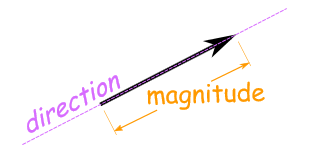
\includegraphics[width=0.5\linewidth]{vec}
\end{center}
\end{frame}

%%%%%%%%%%%%%%%%%%%%%%%%%%%%%%%%%%%%%%%%%%%%%%%%%%%%%%%%%%%
 \begin{frame}[fragile] \frametitle{Vector Addition}

\begin{center}
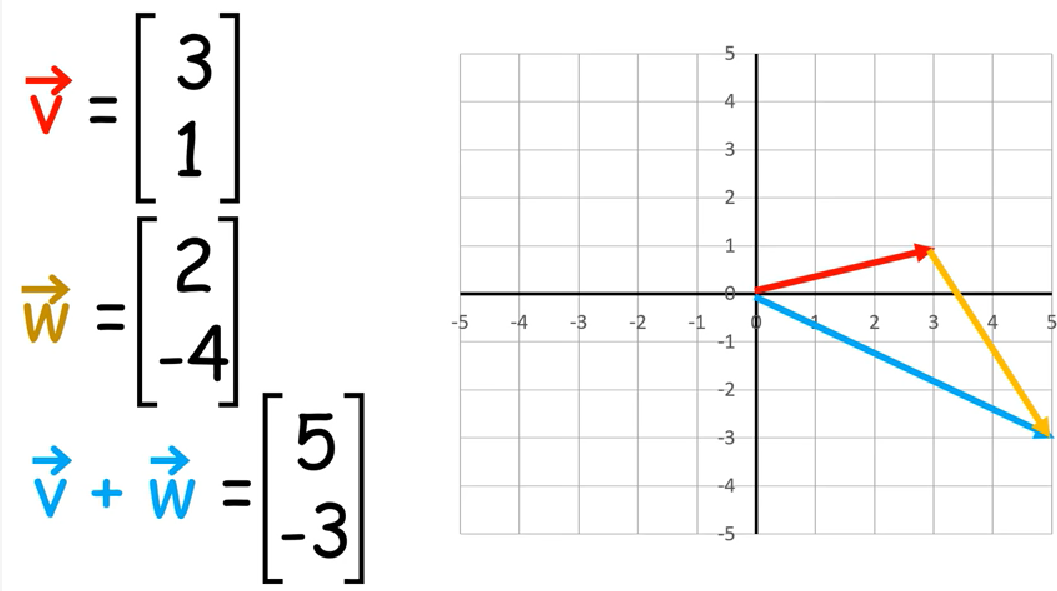
\includegraphics[width=0.5\linewidth,keepaspectratio]{vec1}
\end{center}

\begin{itemize}
\item To add these vectors: We just add the individual components, so 3 plus 2
is 5; and 1 plus -4 is -3.
\item It is simply adding another leg to the journey; so if
we follow vector V along 3 and up 1, and then follow vector W along 2 and down 4,
we end up at the head of the vector we calculated by adding V and
W together.
\end{itemize}

\end{frame}


%%%%%%%%%%%%%%%%%%%%%%%%%%%%%%%%%%%%%%%%%%%%%%%%%%%%%%%%%%%
  \begin{frame}[fragile]{Vector Addition}
 \textbf{Definition}
    We define the sum and  of two vectors by 
     \[
      \left[\begin{array}{r}
       u_1 \\ u_2 \\ \vdots \\ u_n
      \end{array}\right]
    +
    \left[\begin{array}{r}
       v_1 \\ v_2 \\ \vdots \\ v_n
      \end{array}\right]
     = 
     \left[\begin{array}{r}
       u_1 + v_1  \\ u_2 + v_2 \\ \vdots \\ u_n + v_n
      \end{array}\right]
    \]     
    and the product of a scalar and a vector by
    \[
     \alpha \left[\begin{array}{r}
       u_1 \\ u_2 \\ \vdots \\ u_n
      \end{array}\right]
    =  
    \left[\begin{array}{r}
       \alpha u_1 \\ \alpha u_2 \\ \vdots \\ \alpha u_n
      \end{array}\right]
    \]
 
\end{frame}

%%%%%%%%%%%%%%%%%%%%%%%%%%%%%%%%%%%%%%%%%%%%%%%%%%%%%%%%%%%
\begin{frame}[fragile]\frametitle{Example}

  \[
  \left[\begin{array}{r}
   1 \\ 3 \\ -5
  \end{array}\right]
+
\left[\begin{array}{r}
   2 \\ 2 \\ 7
  \end{array}\right]
 =   
 \left[\begin{array}{r}
    3 \\ 5 \\ 2 
  \end{array}\right]   
  \qquad 
  \mbox{ and } \qquad  
   3 \left[\begin{array}{r}
   5 \\ 2 \\ 1
  \end{array}\right]
=  
\left[\begin{array}{r} 15 \\ 6 \\ 3  \end{array}\right]
\]
  
\end{frame}


%%%%%%%%%%%%%%%%%%%%%%%%%%%%%%%%%%%%%%%%%%%%%%%%%%%%%%%%%%%
\begin{frame}[fragile]\frametitle{Exercise}

Let $\vec{u}$ and $\vec{v}$ be given by 
\[
 \vec{u} = \left[\begin{array}{r} 1 \\ 1 \end{array}\right]
 \qquad \mbox{and} \qquad
 \vec{v} = \left[\begin{array}{r} 1 \\ -1 \end{array}\right]
\]
Plot  $\vec{u}$, $\vec{v}$, $\vec{2u}$ and 
$\vec{u}+\vec{v}$.


\textbf{Parallelogram rule for vector addition}
Suppose $\vec{u}$ and $\vec{v}\in \mathbb R^2$.  Then 
$\vec{u}+\vec{v}$ corresponds to the fourth vertex
of the parallelogram whose opposite vertex is $\vec{0}$
and whose other two vertices are $\vec{u}$ and $\vec{v}$.

\end{frame}

%%%%%%%%%%%%%%%%%%%%%%%%%%%%%%%%%%%%%%%%%%%%%%%%%%%%%%%%%%%
\begin{frame}[fragile]\frametitle{Exercise}

     Let $\vec{u} = \left[\begin{array}{r} 6 \\3 \end{array}\right]$
    and $\vec{v} = \left[\begin{array}{r} 5 \\2 \end{array}\right]$.  Display 
    $\vec{u}$, $-2/3\vec{u}$, $\vec{v}$ and $-2/3\vec{u} + \vec{v}$
    on a graph.
  
\end{frame}

%%%%%%%%%%%%%%%%%%%%%%%%%%%%%%%%%%%%%%%%%%%%%%%%%%%%%%%%%%%
  \begin{frame}[fragile]\frametitle{ $\mathbb R^n$}
In general we will consider vectors in $\mathbb R^n$, that is, having $n$ real entries.
$
 \vec{u} = \left[\begin{array}{r} u_1 \\ u_2\\ \vdots \\ u_n \end{array}\right] \in \mathbb R^n
$

The zero vector is $\vec{0} = \left[\begin{array}{r} 0 \\ 0 \\ \vdots \\ 0 \end{array}\right]$
having $n$ entries, each equal to $0$.
\end{frame}

%%%%%%%%%%%%%%%%%%%%%%%%%%%%%%%%%%%%%%%%%%%%%%%%%%%%%%%%%%%
  \begin{frame}[fragile]\frametitle{Properties of $R^n$}
\textbf{Theorem}  Suppose that $\vec{u}, \vec{v},\vec{w}\in \mathbb R^n$ and $c,d\in \mathbb R$.  Then,
\begin{itemize}
 \item $\vec{u} + \vec{v} = \vec{v} + \vec{u}$.
 \item $(\vec{u} + \vec{v} ) + \vec{w} = 
        \vec{u} + ( \vec{v} + \vec{w})$
 \item $\vec{u} + \vec{0} = \vec{0} +\vec{u} = \vec{u}$
 \item $\vec{u} + -\vec{u} = -\vec{u}+ \vec{u} = \vec{0}$
 $\qquad \qquad$ ($\ -\vec{u} = (-1)\vec{u}\ $)
 \item $c(\vec{u} + \vec{v} ) = c\vec{u} + c\vec{v}$
 \item $(c+d)\vec{u} = c\vec{u} + d\vec{u}$
 \item $c(d\vec{u}) = (cd)\vec{u}$
 \item $1 \cdot \vec{u} =\vec{u}$
\end{itemize}


\end{frame}

%%%%%%%%%%%%%%%%%%%%%%%%%%%%%%%%%%%%%%%%%%%%%%%%%%%%%%%%%%%%%%%%%%%%%%%%%%%%%%%%%%
 \begin{frame}[fragile]\frametitle{}
\begin{center}
{\Large Vector Multiplication}
\end{center}
\end{frame}

%%%%%%%%%%%%%%%%%%%%%%%%%%%%%%%%%%%%%%%%%%%%%%%%%%%%%%%%%%%%%%%%%%%%%%%%%%%%%%%%%%
\begin{frame}[fragile] \frametitle{Vector Multiplication}

Vector Multiplication is slightly complicated that plain Vector Addition. 

There are a few types of it.

\begin{itemize}
\item Scalar into Vector resulting in a vector: e.g. You have a list (a vector) of people's income. Tax rate is 15\%. How do you get a list of Tax amounts?
\item Vector into Vector resulting in a scalar: e.g. You have different amounts of foreign currencies. You know each ones conversion-to-INR rate. How do you compute total INRs you have?
\item Vector into Vector resulting in a vector: e.g. Area of a parallelogram with a right hand rule direction.
\end{itemize}

\end{frame}


%%%%%%%%%%%%%%%%%%%%%%%%%%%%%%%%%%%%%%%%%%%%%%%%%%%%%%%%%%%%%%%%%%%%%%%%%%%%%%%%%%
 \begin{frame}[fragile]\frametitle{}
\begin{center}
{\Large Scalar Vector Multiplication}
\end{center}
\end{frame}


%%%%%%%%%%%%%%%%%%%%%%%%%%%%%%%%%%%%%%%%%%%%%%%%%%%%%%%%%%%
 \begin{frame}[fragile] \frametitle{Scalar Vector Multiplication}

\begin{center}
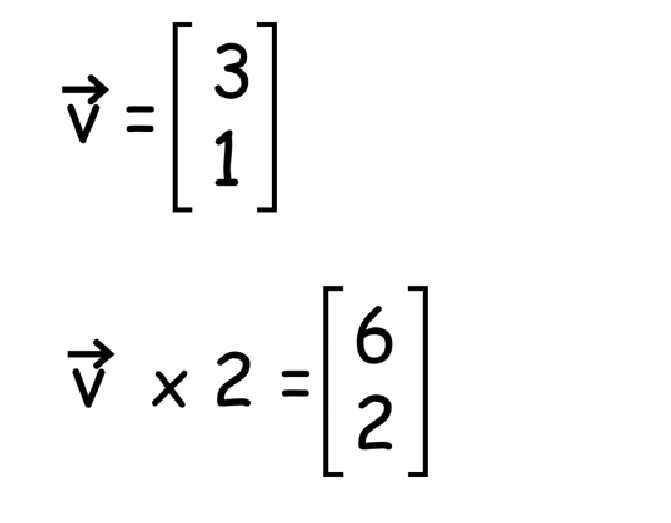
\includegraphics[width=0.5\linewidth,keepaspectratio]{vec2}
\end{center}

Multiply each element of the vector by the scalar
 
\end{frame}

%%%%%%%%%%%%%%%%%%%%%%%%%%%%%%%%%%%%%%%%%%%%%%%%%%%%%%%%%%%
 \begin{frame}[fragile] \frametitle{Scalar Vector Multiplication}

 \begin{lstlisting}
import numpy as np
import matplotlib.pyplot as plt
import math

v = np.array([2,1])

w = 2 * v
print(w)

# Plot w
origin = [0], [0]
plt.grid()
plt.ticklabel_format(style='sci', axis='both', scilimits=(0,0))
plt.quiver(*origin, *w, scale=10)
plt.show()
 \end{lstlisting}
 

 
\end{frame}

%%%%%%%%%%%%%%%%%%%%%%%%%%%%%%%%%%%%%%%%%%%%%%%%%%%%%%%%%%%
 \begin{frame}[fragile] \frametitle{Scalar Vector Multiplication}


\begin{center}
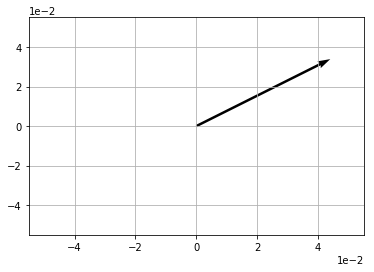
\includegraphics[width=0.5\linewidth,keepaspectratio]{vec5}
\end{center}

 
\end{frame}

%%%%%%%%%%%%%%%%%%%%%%%%%%%%%%%%%%%%%%%%%%%%%%%%%%%%%%%%%%%
 \begin{frame}[fragile] \frametitle{Scalar Vector Multiplication}

 $\vec{b} = \frac{\vec{v}}{2}$
 
 \begin{lstlisting}
b = v / 2
print(b)

# Plot b
origin = [0], [0]
plt.axis('equal')
plt.grid()
plt.ticklabel_format(style='sci', axis='both', scilimits=(0,0))
plt.quiver(*origin, *b, scale=10)
plt.show()
 \end{lstlisting}
 
[1.  0.5]
 
\end{frame}

%%%%%%%%%%%%%%%%%%%%%%%%%%%%%%%%%%%%%%%%%%%%%%%%%%%%%%%%%%%
 \begin{frame}[fragile] \frametitle{Scalar Vector Multiplication}


\begin{center}
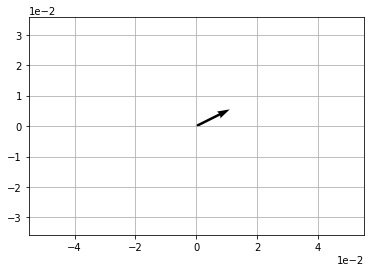
\includegraphics[width=0.5\linewidth,keepaspectratio]{vec6}
\end{center}

 
\end{frame}



%%%%%%%%%%%%%%%%%%%%%%%%%%%%%%%%%%%%%%%%%%%%%%%%%%%%%%%%%%%%%%%%%%%%%%%%%%%%%%%%%%
 \begin{frame}[fragile]\frametitle{}
\begin{center}
{\Large Dot Product}
\end{center}
\end{frame}



%%%%%%%%%%%%%%%%%%%%%%%%%%%%%%%%%%%%%%%%%%%%%%%%%%%%%%%%%%%
 \begin{frame}[fragile] \frametitle{Vector Vector Multiplication}
Dot Product
\begin{center}
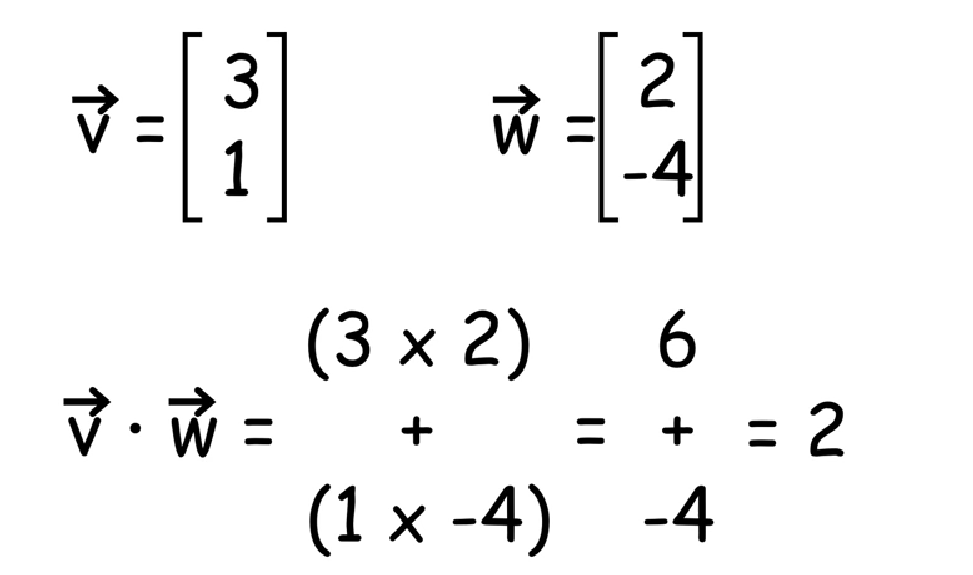
\includegraphics[width=0.5\linewidth,keepaspectratio]{vec3}
\end{center}

Multiply the corresponding elements of the vectors and add the results In this
case, 3 times 2 is 6, and 1 times -4 is -4; and adding these together
gives us our scalar result of 2. 

\end{frame}


%%%%%%%%%%%%%%%%%%%%%%%%%%%%%%%%%%%%%%%%%%%%%%%%%%%%%%%%%%%
 \begin{frame}[fragile] \frametitle{Vector Vector Multiplication}

$\vec{v} \cdot \vec{s} = (v_{1} \cdot s_{1}) + (v_{2} \cdot s_{2}) ... + \; (v_{n} \cdot s_{n})$
 
 \begin{lstlisting}
import numpy as np

v = np.array([2,1])
s = np.array([-3,2])
d = np.dot(v,s)
print (d)
 \end{lstlisting}
 
-4
 
\end{frame}


%%%%%%%%%%%%%%%%%%%%%%%%%%%%%%%%%%%%%%%%%%%%%%%%%%%%%%%%%%%
 \begin{frame}[fragile] \frametitle{Vector Vector Multiplication}

 \begin{itemize}
 
\item Another form: $\vec{v} \cdot \vec{s} = \|\vec{v} \|\|\vec{s}\| \cos (\theta)$ 

\item So for our vectors v (2,1) and s (-3,2), our calculation looks like this:

\item $\cos(\theta) = \frac{(2 \cdot-3) + (-3 \cdot 2)}{\sqrt{2^{2} + 1^{2}} \times \sqrt{-3^{2} + 2^{2}}}$

\item So $\cos(\theta) = -0.496138938357$

\item $\theta \approx 119.74$
\end{itemize}
 
\end{frame}

%%%%%%%%%%%%%%%%%%%%%%%%%%%%%%%%%%%%%%%%%%%%%%%%%%%%%%%%%%%
 \begin{frame}[fragile] \frametitle{Angle Between Two Vectors}

 \begin{itemize}
 
\item Suppose we have two vectors $\vec{v} = (v, 0)$ lying on X axis and $\vec{w}= (w_1,w_2)$
\item $w_1 = ||\vec{w}||cos\theta$, so $\theta = cos^{-1}(\frac{w_1}{||\vec{w}||})$
\item Now, dot product is given as $\vec{v}\cdot\vec{w} = v_1.w_1 + 0.w_2 = v_1.w_1$
\item Putting value of $w_1$, eqn becomes $= v_1.||\vec{w}||cos\theta = ||\vec{v}||||\vec{w}||cos\theta$
\item Therefore: $cos\theta = \frac{\vec{v}\cdot\vec{w}}{||\vec{v}||||\vec{w}||}$
\item Applicable to Higher Dimensions also!!
\end{itemize}
 
\end{frame}

%%%%%%%%%%%%%%%%%%%%%%%%%%%%%%%%%%%%%%%%%%%%%%%%%%%%%%%%%%%%%%%%%%%%%%%%%%%%%%%%%%
\begin{frame}[fragile] \frametitle{Definition}

Suppose that $\vec{u}, \vec{v}\in \mathbb R^n$.  We define the
 \textbf{inner product} or \textbf{dot procuct} or $\vec{u}$ and $\vec{v}$ as
 $$
 u\cdot v = u^tv=\sum_{i=1}^n u_i v_i.
 $$


\textbf{Example}
$$
 \left[ \begin{array}{r} 1\\2\\3 \end{array}\right] \cdot   \left[\begin{array}{r} -1\\-2\\1 \end{array}\right] =
 (1)(-1) + (2)(-2) + (3)(1) = -2.
 $$

\end{frame}

%%%%%%%%%%%%%%%%%%%%%%%%%%%%%%%%%%%%%%%%%%%%%%%%%%%%%%%%%%%%%%%%%%%%%%%%%%%%%%%%%%
\begin{frame}[fragile] \frametitle{Theorem}

Let $\vec{u}, \vec{v}, \vec{w} \in \mathbb R^n$ and let $c$  be a scalar.
Then 
\begin{itemize}
 \item $\vec{u}\cdot \vec{v} = \vec{v} \cdot \vec{u}$.
\item $(\vec{u} + \vec{v})\cdot \vec{w} = \vec{u}\cdot \vec{w}
+\vec{v}\cdot \vec{w}$.
\item $(c \vec{u})\cdot \vec{v}= c (\vec{u}\cdot \vec{v})$.
\item $\vec{u} \cdot \vec{u} \geq 0$ and $\vec{u}\cdot \vec{u} = 0$ 
if and only if $\vec{u} = \vec{0}$.
\item $(c_1 \vec{u}_1 +\dots + c_p \vec{u}_p)\cdot \vec{w} = c_1\vec{u}_1\cdot \vec{w}
+c_p\vec{u}_p\cdot \vec{w}$.
\end{itemize}
 

\textbf{Definition}[Length]
The {\em length} (or {\em norm})  of $\vec{v}$ is the non-negative scalar $\|\vec{v}\|$ 
defined by 
\[
 \| \vec{v} \| = \sqrt{\vec{v} \cdot \vec{v}} =
\sqrt{v_1^2 + v_2^2 +\dots + v_n^2} \ \text{ and } \ \|\vec{v} \|^2 = 
\vec{v}\cdot \vec{v}.
 \]

\end{frame}


%%%%%%%%%%%%%%%%%%%%%%%%%%%%%%%%%%%%%%%%%%%%%%%%%%%%%%%%%%%%%%%%%%%%%%%%%%%%%%%%%%
\begin{frame}[fragile] \frametitle{Note}
 This definition is chosen so that the Pythagorean theorem holds (that is, in two 
dimensions the length $c$ of the vector which is the hypotenuse of a right triangle 
with horizontal length $a$ and vertical height $b$ satisfies $a^2 + b^2 = c^2$. 
 

\textbf{Facts}
\begin{itemize}
 \item For any scalar $c$, $\| c\vec{v}\| = |c| \ \|\vec{v}\|$.  
 \item A vector of length 1 is called a \textbf{unit vector}.  
 \item  If $\vec{v}\neq \vec{0}$ then $\frac{1}{\| \vec{v} \|} \vec{v}$ 
is a unit vector and is in the same direction as $\vec{v}$.   
 \item  The above process is called normalizing. 
\end{itemize}

\end{frame}


%%%%%%%%%%%%%%%%%%%%%%%%%%%%%%%%%%%%%%%%%%%%%%%%%%%%%%%%%%%%%%%%%%%%%%%%%%%%%%%%%%
\begin{frame}[fragile] \frametitle{Example}
 Find a unit vector which is in the same direction as $\vec{v} =
\left[ \begin{array}{rrrr} 1 \\ 1 \\ 2 \end{array} \right]$.
 

\textbf{Definition}
For $\vec{u}$ and $\vec{v}$ in $\mathbb R^n$, the {\em distance between $\vec{u}$
and $\vec{v}$}, written as $\text{dist}(\vec{u},\vec{v})$ is the length
of the vector $\vec{u}-\vec{v}$.  That is,
\[
 \text{dist}(\vec{u},\vec{v})  = \| \vec{u} - \vec{v} \|.
\]
  

\textbf{Example}
 Compute the distance 
$\text{dist}\left[\left[ \begin{array}{rrrr}7 \\ 2 \end{array} \right],\left[ \begin{array}{rrrr} 4 \\ 3 \end{array} \right]\right]$.

\end{frame}

%%%%%%%%%%%%%%%%%%%%%%%%%%%%%%%%%%%%%%%%%%%%%%%%%%%%%%%%%%%%%%%%%%%%%%%%%%%%%%%%%%
\begin{frame}[fragile] \frametitle{Orthogonal Vectors}
 Two vectors in $\mathbb R^n$ are {\em orthogonal} if and only if $\vec{u}\cdot\vec{v}=0$.

\begin{itemize}
\item Angle between two vectors is 0, meaning $cos\theta = 0$ meaning $\theta = 90$ degrees.
\item In 2D, there will be two such orthogonal (perpendicular) vectors to a given vector.
\item if the given vector is 3D, there will be infinite such orthogonal vectors, but all will lie in a single plane.
\item In higher dimensions, the orthogonal entity is called as a Hyperplane, all passing through base of the vector.
\item Hyperplane separates space into 2  halves.
\end{itemize}

\end{frame}

%%%%%%%%%%%%%%%%%%%%%%%%%%%%%%%%%%%%%%%%%%%%%%%%%%%%%%%%%%%%%%%%%%%%%%%%%%%%%%%%%%
\begin{frame}[fragile] \frametitle{Orthogonal Vectors}
 Two vectors in $\mathbb R^n$ are {\em orthogonal} if and only if $\vec{u}\cdot\vec{v}=0$.
  

\textbf{Note}
\begin{eqnarray*}
 \| \vec{u} -\vec{v}\|^2 & =  & (\vec{u}-\vec{v})\cdot(\vec{u}- \vec{v})\\
& = & \vec{u}\cdot \vec{u} - \vec{u} \cdot \vec{v} 
      - \vec{v} \cdot \vec{u} + \vec{v}\vec{v} \\
& = & \| \vec{u} \|^2 + \| \vec{v}\|^2 - 2 \vec{u}\cdot\vec{v}
\end{eqnarray*}


\textbf{Theorem}[Pythagorus]
 $||\vec{u} - \vec{v}||^2 = ||\vec{u}||^2 + ||\vec{v}||^2$ if and only if $\vec{u}$ and $\vec{v}$ are orthogonal.


\end{frame}

%%%%%%%%%%%%%%%%%%%%%%%%%%%%%%%%%%%%%%%%%%%%%%%%%%%%%%%%%%%%%%%%%%%%%%%%%%%%%%%%%%
\begin{frame}[fragile] \frametitle{Definition}

Suppose that $W\le \mathbb R^n$.
\begin{itemize}
  \item  If for all $\vec{w}\in W$, $\vec{z}\cdot\vec{w}=0$,l then we say that $\vec{z}$ is orthogonal to $W$ and write $z\perp W$.
  \item We define the orthogonal compliment of $W$ as $W^{\perp}=\{\vec{z}\in \mathbb R^n \vec{z}\perp W\}$.
\end{itemize}
  

\textbf{Example}
 Suppose that $W=\mbox{Span} \left(\left(\begin{array}{r}1\\0\\0\end{array}\right), \left(\begin{array}{r} 0\\1\\0\end{array}\right)  \right)$.  \\
 Describe $W^{\perp}$.

\end{frame}


%%%%%%%%%%%%%%%%%%%%%%%%%%%%%%%%%%%%%%%%%%%%%%%%%%%%%%%%%%%%%%%%%%%%%%%%%%%%%%%%%%
\begin{frame}[fragile] \frametitle{Fact}
\begin{itemize}
  \item $\vec{x}\in W^{\perp}$ if and only if $\vec{x}\perp \vec{w}$ for all $\vec{w}$ in a spanning set for $W$.
  \item  $W^{\perp}\le \mathbb R^n$.
\end{itemize}
  

\textbf{Theorem}
 Suppose that $A$ is an $n\times n$ matrix.
\begin{itemize}
  \item $(\mbox{Row}(A))^{\perp} = \mbox{Nul}(A)$.
  \item $(\mbox{Col}(A))^{\perp}=\mbox{Nul}(A^t)$.
\end{itemize}

\end{frame}


%%%%%%%%%%%%%%%%%%%%%%%%%%%%%%%%%%%%%%%%%%%%%%%%%%%%%%%%%%%%%%%%%%%%%%%%%%%%%%%%%%
\begin{frame}[fragile] \frametitle{Note}
 In two or three dimensions, the projection of $\vec{v}$ onto $\vec{u}$
has length $\| \vec{v} \| \cos \theta$, where $\theta$ is the angle between
the vectors.  Hence
\[
 \| \vec{v} \| \cos \theta = c \| \vec{u} \|
\]
so that 
\[
 \vec{u}\cdot\vec{v} = \| \vec{u} \| \| \vec{v} \| \cos \theta.
\]
In higher dimensions than three we use this to {\em define} the angle between two vectors.

\end{frame}

%%%%%%%%%%%%%%%%%%%%%%%%%%%%%%%%%%%%%%%%%%%%%%%%%%%%%%%%%%%%%%%%%%%%%%%%%%%%%%%%%%
\begin{frame}[fragile] \frametitle{Definition}
 Two vectors in $\mathbb R^n$ are {\em orthogonal} if and only if $\vec{u}\cdot\vec{v}=0$.
  

\textbf{Note}
\begin{eqnarray*}
 \| \vec{u} -\vec{v}\|^2 & =  & (\vec{u}-\vec{v})\cdot(\vec{u}- \vec{v})\\
& = & \vec{u}\cdot \vec{u} - \vec{u} \cdot \vec{v} 
      - \vec{v} \cdot \vec{u} + \vec{v}\vec{v} \\
& = & \| \vec{u} \|^2 + \| \vec{v}\|^2 - 2 \vec{u}\cdot\vec{v}
\end{eqnarray*}
 

\textbf{Theorem}[Pythagorus]
 $||\vec{u} - \vec{v}||^2 = ||\vec{u}||^2 + ||\vec{v}||^2$ if and only if $\vec{u}$ and $\vec{v}$ are orthogonal.


\end{frame}



\newcommand{\R}{\mathbb{R}}

\newcommand{\norm}[1]{\lVert#1\rVert} % norm

\newcommand{\avg}[1]{\left< #1 \right>} % average

\newcommand{\sabs}[1]{\left| #1 \right|} % smaller absolute value
\newcommand{\abs}[1]{\bigl| #1 \bigr|} % absolute value



%%%%%%%%%%%%%%%%%%%%%%%%%%%%%%%%%%%%%%%%%%%%%%%%%%%%%%%%%%%%%%%%%%%%%%%%%%%%%%%%%%
\begin{frame}[fragile] \frametitle{Inner products}

\textbf{Definition}: An {\em inner product} on a real vector space $V$ is an operation (function) that assigns to each pair of vectors $(\vec{u}, \vec{v})$ in $V$ a \textbf{scalar} $\avg{ \vec{u}, \vec{v} }$ satisfying the following axioms:

\begin{itemize}

\item  $\avg{ \vec{u}, \vec{v} } =  \avg{ \vec{v}, \vec{u} } $   \ (Symmetry)

\item   $\avg{ \vec{u} + \vec{v}, \vec{w} }   =  \avg{ \vec{u}, \vec{w} } +  \avg{ \vec{v}, \vec{w} }$  \ (Additivity)

\item  $\avg{ k \, \vec{u}, \vec{v} }  = k  \, \avg{ \vec{u}, \vec{v} }$ \ (Homogeneity)

\item  $\avg{ \vec{v}, \vec{v} } \, \ge 0$  \ and  $\avg{ \vec{v}, \vec{v} } = 0$ iff $\vec{v} = \vec{0}$ \ (Positivity)


\end{itemize}





\textbf{Theorem} (basic properties): Given vectors $\vec{u}, \vec{v}, \vec{w}$ in an inner product space $V$, and a scalar $k$, the following properties hold:

\begin{itemize}

\item $\avg{ \vec{\rm{o}}, \vec{v} } = \avg{ \vec{v}, \vec{\rm{o}} }  = 0$

\item $\avg{ \vec{u} - \vec{v}, \vec{w} }   =  \avg{ \vec{u}, \vec{w} } -  \avg{ \vec{v}, \vec{w} }$

\item $\avg{ \vec{u}, \vec{v} + \vec{w} }   =  \avg{ \vec{u}, \vec{v} } +  \avg{ \vec{u}, \vec{w} }$

\item $\avg{ \vec{u}, \vec{v} - \vec{w} }   =  \avg{ \vec{u}, \vec{v} }  -  \avg{ \vec{u}, \vec{w} }$

\item  $\avg{ \vec{u}, k \vec{ v} }  = k  \, \avg{ \vec{u}, \vec{v} }$

\end{itemize}

\end{frame}


%%%%%%%%%%%%%%%%%%%%%%%%%%%%%%%%%%%%%%%%%%%%%%%%%%%%%%%%%%%%%%%%%%%%%%%%%%%%%%%%%%
 \begin{frame}[fragile]\frametitle{Norm and distance in an inner product space}

\textbf{Definition}: If $V$ is a real inner product space then we define

\begin{itemize}

\item The norm (or length) of $\vec{v}$:
$$\norm{\vec{v}} = \sqrt{ \avg{ \vec{v}, \vec{v} } } $$

\item The distance between $\vec{u}$ and $\vec{v}$:
$$ d (\vec{u}, \vec{v}) = \norm{ \vec{u} - \vec{v}} =  \sqrt{ \avg{ \vec{u} - \vec{v}, \vec{u} - \vec{v} } } $$

\end{itemize}



\textbf{Theorem} (basic properties): Given vectors $\vec{u}, \vec{v}$ in an inner product space $V$, and a scalar $k$, the following properties hold:

\begin{itemize}

\item $\norm{\vec{v}} \ge 0$ \ and \ $\norm{\vec{v}} = 0$ iff $\vec{v} = \vec{0}$.

\item $\norm{ k \vec{v}} = |k| \, \norm{\vec{v}}$

\item $d (\vec{u}, \vec{v}) = d (\vec{v}, \vec{u}) $

\item $d (\vec{u}, \vec{v} ) \ge 0$ \ and \ $d (\vec{u}, \vec{v}) = 0$ iff $\vec{u} = \vec{v}$.


\end{itemize}

\end{frame}


%%%%%%%%%%%%%%%%%%%%%%%%%%%%%%%%%%%%%%%%%%%%%%%%%%%%%%%%%%%%%%%%%%%%%%%%%%%%%%%%%%
 \begin{frame}[fragile]\frametitle{Angle between vectors}

\textbf{Theorem} (Cauchy-Schwarz): If $u$ and $v$ are vectors in an inner vector space, then
$$\abs{ \avg{u, v} } \le \norm{u} \, \norm{v} $$




\textbf{Definition}: The angle between two vectors  $u$ and $v$ in an inner vector space is defined as
$$\theta = \cos^{-1} \, \frac{\avg{u,v}}{\norm{u} \, \norm{v}}  $$





\textbf{Theorem} (the triangle inequality):  If $u, v$ and $w$ are vectors in an inner vector space, then
\begin{itemize}
\item $\norm{u + v} \le \norm{u} + \norm{v}$

\item $d (u, v) \le d (u, w) + d (w, v)$
\end{itemize}

\end{frame}


%%%%%%%%%%%%%%%%%%%%%%%%%%%%%%%%%%%%%%%%%%%%%%%%%%%%%%%%%%%
 \begin{frame}[fragile] \frametitle{Orthogonality}
\textbf{Definition}:  Two vectors  $u$ and $v$ in an inner vector space are called {\em orthogonal} if $\avg{u, v} = 0$.
\smallskip
Clearly $u \perp v$ iff the angle between them is $\theta = \frac{\pi}{2}$.
\textbf{Theorem} (the Pythagorean theorem):  If $u$ and $v$ are \textbf{orthogonal} vectors in an inner vector space, then
$$\norm{u + v}^2 = \norm{u}^2 + \norm{v}^2$$
\end{frame}

%%%%%%%%%%%%%%%%%%%%%%%%%%%%%%%%%%%%%%%%%%%%%%%%%%%%%%%%%%%%%%%%%%%%%%%%%%%%%%%%%%
\begin{frame}[fragile]\frametitle{Orthogonality}
\textbf{Definition}:  Let $W$ be a subspace of an inner product space $V$. 
The set of vectors in $V$ which are orthogonal to \textbf{every} vector in $W$ is called the {\em orthogonal complement} of $W$ and it is denoted by $W^\perp$.
\textbf{Theorem}: The orthogonal complement has the following properties:
\begin{itemize}
\item $W^\perp$ is a subspace of $V$.
\item $W \cap W^\perp = \{ \vec{\rm{o}} \}$.
\item If $V$ has finite dimension then $(W^\perp)^\perp = W$.
\end{itemize}
\end{frame}

%%%%%%%%%%%%%%%%%%%%%%%%%%%%%%%%%%%%%%%%%%%%%%%%%%%%%%%%%%%%%%%%%%%%%%%%%%%%%%%%%%
 \begin{frame}[fragile]\frametitle{Orthogonal sets, orthonormal sets}
Let $(V, \avg{ \ })$ be an inner product space and let $S$ be a set of vectors in $V$.
\textbf{Definition}: The set $S$  is called {\em orthogonal} if any two vectors in $S$  are orthogonal.
The set $S$ is called {\em orthonormal} if it is orthogonal and any vector in $S$ has norm $1$.
\textbf{Theorem}: Every orthogonal set of nonzero vectors is linearly independent.

\end{frame}

%%%%%%%%%%%%%%%%%%%%%%%%%%%%%%%%%%%%%%%%%%%%%%%%%%%%%%%%%%%%%%%%%%%%%%%%%%%%%%%%%%
 \begin{frame}[fragile]
\frametitle{Orthogonal sets, orthonormal sets}
\textbf{Definition}: A set of vectors $S$  is called an {\em orthogonal} basis (OGB) for $V$ if $S$ is a basis and an orthogonal set (that is, $S$ is a basis where all vectors are perpendicular).

A set of vectors $S$  is called an {\em orthonormal} basis (ONB) for $V$ if $S$ is a basis and an orthonormal set (that is, $S$ is a basis where all vectors are perpendicular and have norm $1$).
\end{frame}

%%%%%%%%%%%%%%%%%%%%%%%%%%%%%%%%%%%%%%%%%%%%%%%%%%%%%%%%%%%%%%%%%%%%%%%%%%%%%%%%%%
 \begin{frame}[fragile]\frametitle{Orthogonal sets, orthonormal sets}

Let $(V, \avg{ \ })$ be an inner product space.

\textbf{Theorem}:  If $S = \{ v_1, v_2, \ldots, v_n \}$ is an orthogonal basis in $V$ and $u$ is any vector in $V$, then
$$u = \frac{\avg{u, v_1}}{\norm{v_1}^2} \, v_1 + \frac{\avg{u, v_2}}{\norm{v_2}^2} \, v_2 + \ldots + \frac{\avg{u, v_n}}{\norm{v_n}^2} \, v_n$$

If $S = \{ v_1, v_2, \ldots, v_n \}$ is an orthonormal basis in $V$ and $u$ is any vector in $V$, then
$$u = \avg{u, v_1} \, v_1 + \avg{u, v_2} \, v_2  + \ldots + \avg{u, v_n} \, v_n$$ 

\end{frame}


%%%%%%%%%%%%%%%%%%%%%%%%%%%%%%%%%%%%%%%%%%%%%%%%%%%%%%%%%%%%%%%%%%%%%%%%%%%%%%%%%%
 \begin{frame}[fragile]\frametitle{}
\begin{center}
{\Large Cross Product}
\end{center}
\end{frame}


%%%%%%%%%%%%%%%%%%%%%%%%%%%%%%%%%%%%%%%%%%%%%%%%%%%%%%%%%%%
 \begin{frame}[fragile] \frametitle{Vector Vector Multiplication}
Cross Product (for 3D vectors)
\begin{center}
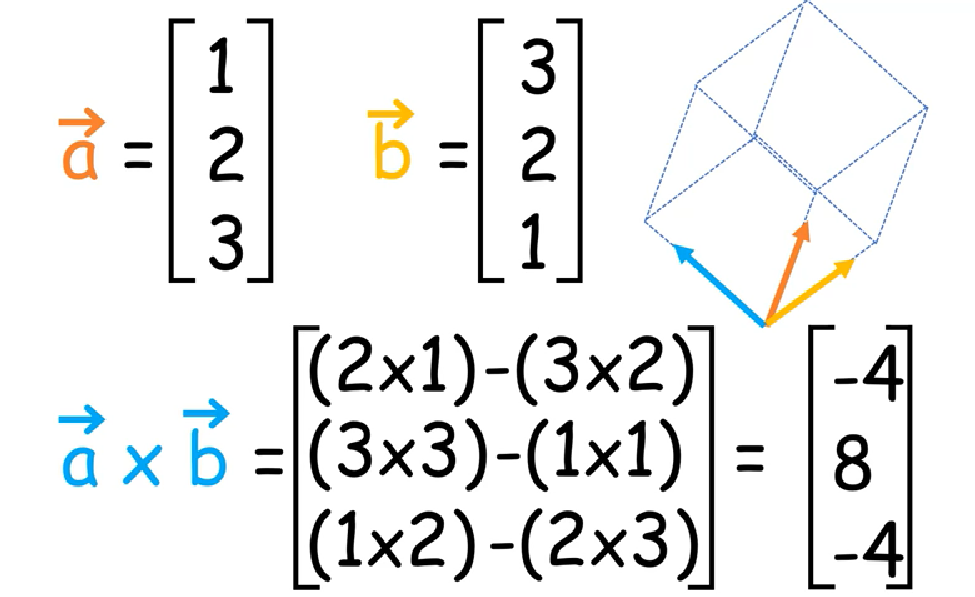
\includegraphics[width=0.5\linewidth,keepaspectratio]{vec4}
\end{center}
Skipping the current row and column, calculate determinant value of remaining sub matrix for that position.
\end{frame}


%%%%%%%%%%%%%%%%%%%%%%%%%%%%%%%%%%%%%%%%%%%%%%%%%%%%%%%%%%%
 \begin{frame}[fragile] \frametitle{Vector Vector Multiplication}
Cross Product
 \begin{itemize}
 
\item $\vec{p} = \begin{bmatrix}2 \\ 3 \\ 1 \end{bmatrix}\;\; \vec{q} = \begin{bmatrix}1 \\ 2 \\ -2 \end{bmatrix}$
\item \begin{align}r_{1} = p_{2}q_{3} - p_{3}q_{2} \\ r_{2} = p_{3}q_{1} - p_{1}q_{3} \\ r_{3} = p_{1}q_{2} - p_{2}q_{1} \end{align}
\item $\vec{r} = \vec{p} \times \vec{q} = \begin{bmatrix}(3 \cdot -2) - (1 \cdot 2) \\ (1 \cdot 1) - (2 \cdot -2) \\ (2 \cdot 2) - (3 \cdot 1) \end{bmatrix} = \begin{bmatrix}-6 - 2 \\ 1 - -4 \\ 4 - 3 \end{bmatrix} = \begin{bmatrix}-8 \\ 5 \\ 1 \end{bmatrix}$
\end{itemize}
 
\end{frame}


%%%%%%%%%%%%%%%%%%%%%%%%%%%%%%%%%%%%%%%%%%%%%%%%%%%%%%%%%%%
 \begin{frame}[fragile] \frametitle{Vector Vector Multiplication}

Cross Product
 
 \begin{lstlisting}
import numpy as np

p = np.array([2,3,1])
q = np.array([1,2,-2])
r = np.cross(p,q)
print (r)
 \end{lstlisting}
 
[-8  5  1]
\end{frame}

%%%%%%%%%%%%%%%%%%%%%%%%%%%%%%%%%%%%%%%%%%%%%%%%%%%%%%%%%%%%%%%%%%%%%%%%%%%%%%%%%%
 \begin{frame}[fragile]\frametitle{}
\begin{center}
{\Large Linear Combinations}
\end{center}
\end{frame}




%%%%%%%%%%%%%%%%%%%%%%%%%%%%%%%%%%%%%%%%%%%%%%%%%%%%%%%%%%%
  \begin{frame}[fragile]\frametitle{Linear Combinations}
\textbf{Definition}
Let $p$ be a positive integer. Given vectors $\vec{u}_1, \vec{u}_2, \dots \vec{u}_p$
in $\mathbb R^n$, and $c_1, c_2, \dots c_p$ in $\mathbb R$, the vector
\[
 \vec{u} = c_1 \vec{u}_1 + c_2 \vec{u}_2 + \dots c_p\vec{u}_p
\]
is called a linear combination of the vectors $\vec{u}_1, \dots \vec{u}_p$ with
weights $c_1, \dots c_p$.

\end{frame}

%%%%%%%%%%%%%%%%%%%%%%%%%%%%%%%%%%%%%%%%%%%%%%%%%%%%%%%%%%%
  \begin{frame}[fragile]
\textbf{Example}
\[
 2\left[\begin{array}{r}1 \\-2 \\ 7  \end{array}\right]\ 
 + \ 3\left[\begin{array}{r} 1 \\ 1 \\ 1 \end{array}\right] \ 
 + \ -2\left[\begin{array}{r}2 \\ 3 \\ -8  \end{array}\right]
 = \left[\begin{array}{r}\qquad  \\ \qquad \\ \qquad \end{array}\right] \]     
is a linear combination of $ \left[\begin{array}{r}1 \\-2 \\ 7  \end{array}\right],$ $\left[\begin{array}{r} 1 \\ 1 \\ 1 \end{array}\right]$ and $\left[\begin{array}{r}2 \\ 3 \\ -8  \end{array}\right]$ with weights $2,3 ,-2$.


\textbf{Geometry} 
Let $\vec{u} = \left[\begin{array}{r} 1 \\ 1 \end{array}\right]$ and 
$\vec{v} = \left[\begin{array}{r} 1 \\ -1 \end{array}\right]$.  Show all
linear combinations of $\vec{u}$ and $\vec{v}$ on a graph.

\end{frame}

%%%%%%%%%%%%%%%%%%%%%%%%%%%%%%%%%%%%%%%%%%%%%%%%%%%%%%%%%%%
  \begin{frame}[fragile]
\textbf{Exercise}
let 
$\vec{u}_1 = \left[\begin{array}{r} 1 \\ 2 \\ 5 \end{array}\right]$
$\vec{u}_2 = \left[\begin{array}{r} 2 \\ 1 \\ 3 \end{array}\right]$ and 
$\vec{b} = \left[\begin{array}{r} -4 \\ 1 \\ 1 \end{array}\right]$
Is $\vec{b}$ a linear combination of $\vec{u}_1$ and $\vec{u}_2$

\end{frame}

%%%%%%%%%%%%%%%%%%%%%%%%%%%%%%%%%%%%%%%%%%%%%%%%%%%%%%%%%%%
  \begin{frame}[fragile]\frametitle{Vector Equations}
\textbf{Facts}
A vector equation 
\[
 x_1 \vec{v}_1  + x_2 \vec{v}_2 + \dots + x_n \vec{v}_n =\vec{b}
\]
has the same solution set as the system of equations whose augmented matrix is 
\[
 \left[\begin{array}{ccccc}
  | & | & \dots & | & | \\
  \vec{v}_1 & \vec{v}_2 & \dots & \vec{v}_n & \vec{b} \\
  | & | & \dots & | & | \\
 \end{array}\right]
\]
In particular, $\vec{b}$ is a linear combination of $\vec{v}_1, \dots \vec{v}_n$
if and only if the system of linear equations is consistent.

\end{frame}

%%%%%%%%%%%%%%%%%%%%%%%%%%%%%%%%%%%%%%%%%%%%%%%%%%%%%%%%%%%
  \begin{frame}[fragile]
\textbf{Definition}
 Suppose $\vec{v}_1, \vec{v}_2, \dots \vec{v}_p \in \mathbb R^n$.
 We define 
 \[
  \mbox{Span}(\vec{v}_1, \vec{v}_2, \dots ,\vec{v}_p) =
 \left\{
 c_1 \vec{v}_1 + c_2 \vec{v}_2 + \dots c_p \vec{v}_p: c_1, c_2, \dots , c_p \in \mathbb R 
 \right\}
 \]    
 That is, Span$(\vec{v}_1, \dots , \vec{v}_p)$ is the set of all linear combinations
of $\vec{v}_1, \dots , \vec{v}_p$.

\end{frame}

%%%%%%%%%%%%%%%%%%%%%%%%%%%%%%%%%%%%%%%%%%%%%%%%%%%%%%%%%%%
  \begin{frame}[fragile]\frametitle{Geometry}
\textbf{Note}
\begin{itemize}
\item The span of $\vec{0}$ in $\mathbb R^2$ or $\mathbb R^3$ is the single point $\vec{0}$.
\item The span of a single non-zero vector in $\mathbb R^2$ or $\mathbb R^3$ is a line through $\vec{0}$.
\item The span of two non-zero vectors in $\mathbb R^3$ is either a plane through $\vec{0}$ or, if one
vector is a scalar multiple of the other, a line through $\vec{0}$.
\end{itemize}


\textbf{Exercise}
Let $\vec{v}_1 = \left[\begin{array}{r}1 \\ 1 \\ 2 \end{array}\right]$, 
$\vec{v}_2 = \left[\begin{array}{r} 2 \\ 5 \\ -3 \end{array}\right]$ and 
$\vec{b} = \left[\begin{array}{r} -9 \\ -30 \\ 31 \end{array}\right]$.
Span$(\vec{v}_1,\vec{v}_2)$ is a plane in $\mathbb R^3$  Is $\vec{b}$ in that plane?

\end{frame}

% %%%%%%%%%%%%%%%%%%%%%%%%%%%%%%%%%%%%%%%%%%%%%%%%%%%%%%%%%%%%%%%%%%%%%%%%%%%%%%%%%%
 \begin{frame}[fragile]\frametitle{}
\begin{center}
{\Large Matrix}
\end{center}
\end{frame}


%%%%%%%%%%%%%%%%%%%%%%%%%%%%%%%%%%%%%%%%%%%%%%%%%%%%%%%%%%%
\begin{frame}[fragile]\frametitle{Meaning of a Matrix}

 \begin{itemize}
  \item Matrix is organization of data into rows and columns
  \item Example: columns can be various aspects of a person, such as height,weight, salary, etc, where as rows can represent different persons 
  \item This Excel sheet like data can be thought of as a Matrix (especially in Data Science, Machine Learning)
 \end{itemize}

\end{frame}



%%%%%%%%%%%%%%%%%%%%%%%%%%%%%%%%%%%%%%%%%%%%%%%%%%%%%%%%%%%
 \begin{frame}[fragile] \frametitle{Matrix }
A matrix is an array of numbers that can be arranged into rows
and columns. We generally name matrices with a capital letter.

$A = \begin{bmatrix}
  1 & 2 & 3 \\
  4 & 5 & 6
 \end{bmatrix}$
 
\begin{lstlisting}
 import numpy as np

A = np.array([[1,2,3],
              [4,5,6]])
print (A)

[[1 2 3]
 [4 5 6]]
\end{lstlisting}


\end{frame}

%%%%%%%%%%%%%%%%%%%%%%%%%%%%%%%%%%%%%%%%%%%%%%%%%%%%%%%%%%%
  \begin{frame}[fragile]\frametitle{Matrix}
\textbf{Definition}
A matrix with $m$ rows and $n$ columns is referred to as an $m \times n$ matrix.
The number of rows always comes before the number of columns.
%Thus the matrices above are $2 \times 2$ and $2 \times 3$ respectively.

$A = \begin{bmatrix}
  a_{1,1} & a_{1,2} & a_{1,3} \\
  a_{2,1} & a_{2,2} & a_{2,3}
 \end{bmatrix}$
 
\begin{lstlisting}
import numpy as np

M = np.matrix([[1,2,3],
               [4,5,6]])
print (M)

[[1 2 3]
 [4 5 6]] 
\end{lstlisting}


\end{frame}


%%%%%%%%%%%%%%%%%%%%%%%%%%%%%%%%%%%%%%%%%%%%%%%%%%%%%%%%%%%
 \begin{frame}[fragile] \frametitle{Matrix Addition}
 You can
add or subtract matrices of the same size by simply adding or subtracting the
corresponding elements in the two matrices. 

\begin{center}
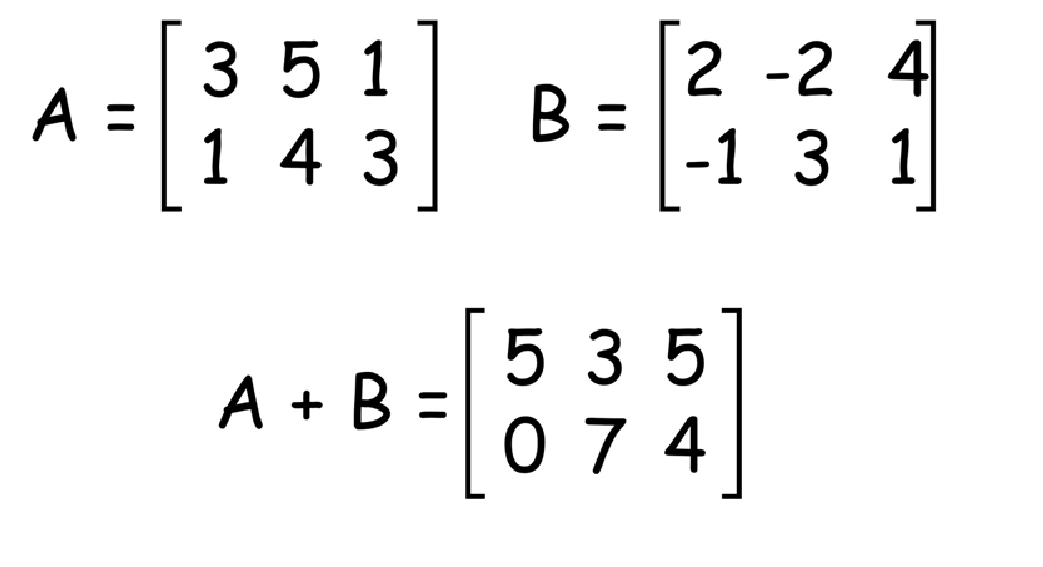
\includegraphics[width=0.5\linewidth,keepaspectratio]{mat1}
\end{center}

$\begin{bmatrix}1 & 2 & 3 \\4 & 5 & 6\end{bmatrix}+ \begin{bmatrix}6 & 5 & 4 \\3 & 2 & 1\end{bmatrix} = \begin{bmatrix}7 & 7 & 7 \\7 & 7 & 7\end{bmatrix}$
\end{frame}

%%%%%%%%%%%%%%%%%%%%%%%%%%%%%%%%%%%%%%%%%%%%%%%%%%%%%%%%%%%
  \begin{frame}[fragile]\frametitle{Matrix Addition}
 
\begin{lstlisting}
import numpy as np

A = np.array([[1,2,3],
              [4,5,6]])
B = np.array([[6,5,4],
              [3,2,1]])
print(A + B)

[[7 7 7]
 [7 7 7]]
\end{lstlisting}

\end{frame}

%%%%%%%%%%%%%%%%%%%%%%%%%%%%%%%%%%%%%%%%%%%%%%%%%%%%%%%%%%%
  \begin{frame}[fragile]\frametitle{Matrix Subtraction}
 
 $\begin{bmatrix}1 & 2 & 3 \\4 & 5 & 6\end{bmatrix}- \begin{bmatrix}6 & 5 & 4 \\3 & 2 & 1\end{bmatrix} = \begin{bmatrix}-5 & -3 & -1 \\1 & 3 & 5\end{bmatrix}$
\begin{lstlisting}
import numpy as np

A = np.array([[1,2,3],
              [4,5,6]])
B = np.array([[6,5,4],
              [3,2,1]])
print(A - B)

[[-5 -3 -1]
 [ 1  3  5]]
\end{lstlisting}

\end{frame}


%%%%%%%%%%%%%%%%%%%%%%%%%%%%%%%%%%%%%%%%%%%%%%%%%%%%%%%%%%%
\begin{frame}[fragile]\frametitle{The Transpose of a Matrix}
\textbf{Definition}
The transpose of a $m\times n$ matrix $A$ is the matrix $A^{T}$ 
having $(i,j)$-entry $a_{ji}$.  That is,
$$(A^{T})_{i j} = a_{j i}.$$



\textbf{Example}
For example, 
$ A = \left[ \begin{array}{rrr}
      1 & 2 & 3 \\
      4 & 5 & 6
     \end{array}\right]$
has transpose  
$A^T = \left[\begin{array}{rrr}
        1 & 4 \\ 
        2 & 5 \\
        3 & 6
       \end{array}\right]$.



\textbf{Note}
The rows of $A$ become the columns of $A^T$ and vice versa.

\end{frame}


%%%%%%%%%%%%%%%%%%%%%%%%%%%%%%%%%%%%%%%%%%%%%%%%%%%%%%%%%%%
\begin{frame}[fragile]\frametitle{Meaning of a Matrix Multiplication}

 \begin{itemize}
  \item Matrix is organization of data into rows and columns
  \item Example: columns can be various aspects of a person, such as height,weight, salary, etc, where as rows can represent different persons 
  \item This Excel sheet like data can be thought of as a Matrix (especially in Data Science, Machine Learning)
  \item If you have another matrix like this, what is the meaning of their multiplication?
  \item Geometrically: say first matrix represents points of a shape, a polygon, where each row is a point, and each column represents X, Y, Z coordinates.
  \item Second matrix is typically a Homogeneous transformation matrix, such as rotation,  when multiplied gets rotated shape.
 \end{itemize}

\end{frame}

%%%%%%%%%%%%%%%%%%%%%%%%%%%%%%%%%%%%%%%%%%%%%%%%%%%%%%%%%%%
\begin{frame}[fragile]\frametitle{Matrix Multiplication Rules}
\textbf{Theorem}  Let $A$ and $B$ be matrices whose sizes are appropriate for the following 
sums and products to be defined
 \begin{itemize}
  \item $(A^T)^T = A$
\item $(A+B)^T = A^T + B^T$.
\item For any scalar $r$, $(rA)^T=rA^T$.
\item $(AB)^T = B^T A^T$
 \end{itemize}


\end{frame}


%%%%%%%%%%%%%%%%%%%%%%%%%%%%%%%%%%%%%%%%%%%%%%%%%%%%%%%%%%%
\begin{frame}[fragile]\frametitle{Example}
  
$A = \begin{bmatrix} 1 & 2 \\ 3 & 4 \end{bmatrix}$, and $B= 
\begin{bmatrix}
 5 & 1 & -1 \\
 1 & 2 & 2 
\end{bmatrix}$
then 
\[
 AB = \begin{bmatrix}
       7 & 5 & 3 \\
       9 & 11 & 5
      \end{bmatrix}
\qquad 
(AB)^T = \begin{bmatrix} 7 & 9 \\
          5 & 11 \\ 3 & 5
         \end{bmatrix} = B^T A^T
\]
but $A^T$ is $2\times 2$ and $B^T$ is $3 \times 2$, so $A^TB^T$ isn't even defined.

\end{frame}


%
%
%
%
%  \begin{frame}[fragile]
%\textbf{Definition}
%Suppose that $T: \mathbb R^n \longrightarrow \mathbb R^m$ is linear.   We will say that 
%$T$ is invertible if for every $\vec{b} \in \mathbb R^m$
%there is exactly one $\vec{x} \in \mathbb R^n$ so that $T(\vec{x})= \vec{b}$.
%
%
%
%\textbf{Note}
%If $T$ is invertible, this means that $T$ is onto 
%(every equation can be solved: hence $m\leq n$) and $T$ is 1-1 (every equation 
%has at most one solution: hence $n \leq m$).  
%
%
%Thus $n=m$ and  an invertible linear transformation has a matrix which must be square.  
%
%
%
%
%\textbf{Questions}
%\begin{itemize}
%\item Which square matrices are invertible? 
%\item What does it mean for a square matrix to be invertible?
%\end{itemize}
%
%\end{frame}
%
%
%
%
%
%
%  \begin{frame}[fragile]
%\textbf{Facts}
%Suppose that $T: \mathbb R^n \longrightarrow \mathbb R^n$ is an invertible linear transformation: then we
%can define $S : \mathbb R^n \longrightarrow \mathbb R^n$ so that $T\vec{x} = \vec{u}$ if and 
%only if $\vec{x}= S(\vec{u})$.  Furthermore, for every vector 
%$\vec{x} \in \mathbb R^n$,  $S(T(\vec{x}))=\vec{x}$, and 
%for every $\vec{u} \in \mathbb R^n$, $T(S(\vec{u}))= \vec{u}$.
%
%
%
%\textbf{Facts}
%It turns out that $S$ must also be linear. 
%\end{frame}
%
%
%
%
%
%  \begin{frame}[fragile]
%\textbf{Proof}
%We'll assume that $T(\vec{x})= \vec{u}$
% and $T(\vec{y})=\vec{v}$.  Then $S(\vec{u}) = \vec{x} $
%and $S(\vec{v} ) =\vec{y}$.
%
%
%Note that
% $S(T(r\vec{x})) = r\vec{x}$,
%so  we get
% \[
%S(r \vec{u}) = S(r T(\vec{x})) = S(T(r \vec{x}))= r\vec{x}
% = r S(\vec{u} ) 
%   \]
%so that $S$ commutes with scalar addition.
%
%
%Likewise,
%\[
% S(\vec{u} + \vec{v}) = 
%S( T(\vec{x}) + T(\vec{y}) ) =
%S ( T (\vec{x} + \vec{y} )) =
%(\vec{x} + \vec{y}) =
%S(\vec{u}) + S(\vec{v})
%\]
% so that $S$ commutes with addition.  
% 
% Thus $S$ is linear.
%
%\end{frame}
%
%
%
%
%
%
%  \begin{frame}[fragile]
%\textbf{Note}
%We see that if $T$ is an invertible linear transformation from $\mathbb R^n$ to $\mathbb R^n$, then so is $S$.  \\ 
%Hence we can represent $T$ by a square matrix $A$ and $S$ by a square matrix $B$.
%
%
%Then $S(T(\vec{x}))= \vec{x}$ for all $\vec{x}$ means that 
%$BA \vec{x}= \vec{x}$ for every $\vec{x}$.  \\ 
%
%In particular, if 
%$C=BA$, then we have $C \vec{e}_j = \vec{e}_j$, so that we obtain that 
%$C$ must be the identity matrix $I_n$.  \\ 
%
%Similarly, $T(S(\vec{u})) = \vec{u}$ for every $\vec{u}$, and hence
%$AB=I_n$ is also the identity matrix.
%
%\end{frame}



%%%%%%%%%%%%%%%%%%%%%%%%%%%%%%%%%%%%%%%%%%%%%%%%%%%%%%%%%%%
 \begin{frame}[fragile] \frametitle{Matrix Transpose}
Exchange rows and columns

\begin{center}
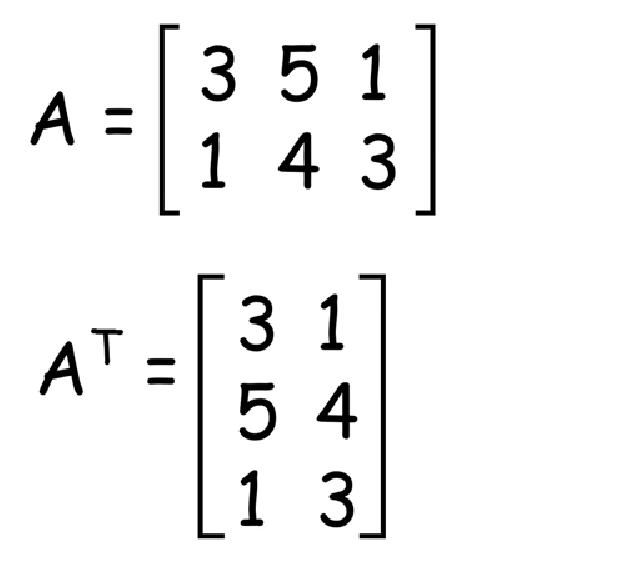
\includegraphics[width=0.5\linewidth,keepaspectratio]{mat2}
\end{center}
\end{frame}

%%%%%%%%%%%%%%%%%%%%%%%%%%%%%%%%%%%%%%%%%%%%%%%%%%%%%%%%%%%
\begin{frame}[fragile]\frametitle{Matrix Transpose}
 
$\begin{bmatrix}1 & 2 & 3 \\4 & 5 & 6\end{bmatrix}^{T} = \begin{bmatrix}1 & 4\\2 & 5\\3 & 6 \end{bmatrix}$

\begin{lstlisting}
import numpy as np

A = np.array([[1,2,3],
              [4,5,6]])
print(A.T)

[[1 4]
 [2 5]
 [3 6]]
\end{lstlisting}

\end{frame}

%%%%%%%%%%%%%%%%%%%%%%%%%%%%%%%%%%%%%%%%%%%%%%%%%%%%%%%%%%%
 \begin{frame}[fragile] \frametitle{Matrix Multiplication}
 Here are the cases to consider:
\begin{itemize}
\item Scalar multiplication, which is
multiplying a matrix by a single number
\item Element wise matrix multiplication (rarely used, called Hadamard multiplication, shown with circle instead of dot)
\item Dot product matrix multiplication, or
multiplying a matrix by another matrix.
\end{itemize}

\end{frame}


%%%%%%%%%%%%%%%%%%%%%%%%%%%%%%%%%%%%%%%%%%%%%%%%%%%%%%%%%%%
 \begin{frame}[fragile] \frametitle{Matrix Scalar Multiplication}
To multiply a matrix by a scalar value, you just multiply each element by the scalar to produce a new matrix:

$2 \times \begin{bmatrix}1 & 2 & 3 \\4 & 5 & 6\end{bmatrix} = \begin{bmatrix}2 & 4 & 6 \\8 & 10 & 12\end{bmatrix}$


\begin{lstlisting}
import numpy as np
import numpy as np

A = np.array([[1,2,3],
              [4,5,6]])
print(2 * A)

[[ 2  4  6]
 [ 8 10 12]]
\end{lstlisting}

\end{frame}

%%%%%%%%%%%%%%%%%%%%%%%%%%%%%%%%%%%%%%%%%%%%%%%%%%%%%%%%%%%
  \begin{frame}[fragile]\frametitle{Matrix Multiplication Defined}
\textbf{Definition}
If $A$ is an $m \times n$ matrix, and if $B=[\vec{b}_1,\vec{b}_2 \dots, \vec{b}_p]$ is a $n\times p$ matrix, then the matrix product
$AB$ is the following $m \times p$ matrix.
\[
 AB = [ A \vec{b}_1 \ \ \  A \vec{b}_2 \ \ \  \dots 
\ \ \  A \vec{b}_p ]
\]



\textbf{Example}
Let $A =\left[\begin{array}{rr} 1& 2 \\ -2 & 3\end{array}\right]$ and let $B=\left[\begin{array}{rrr} 3 & -1 & 6 \\ 7& 5& 3\end{array}\right]$.  Compute $AB$.

\end{frame}





%%%%%%%%%%%%%%%%%%%%%%%%%%%%%%%%%%%%%%%%%%%%%%%%%%%%%%%%%%%
  \begin{frame}[fragile]\frametitle{Multiplying Matrices}
\textbf{Row-Column Rule}
If $A$ is  $m \times n$ and if $B$ is $n\times p$ the $(i,j)$-entry of $AB$ is 
given by 
\[
 (AB)_{ij} = \sum_{k=1}^n a_{ik} b_{kj}
\]



\textbf{Note}
$\mbox{Row}_i(AB) = \mbox{Row}_i(A) \cdot B$.

\end{frame}


%%%%%%%%%%%%%%%%%%%%%%%%%%%%%%%%%%%%%%%%%%%%%%%%%%%%%%%%%%%
 \begin{frame}[fragile] \frametitle{Matrix Dot Product Multiplication}
\begin{itemize}
\item  Multiplying each of the elements in each row of the first matrix by each of the elements in each column of the second matrix and adding the results.
\item  $\begin{bmatrix}1 & 2 & 3 \\4 & 5 & 6\end{bmatrix} \cdot \begin{bmatrix}9 & 8 \\ 7 & 6 \\ 5 & 4\end{bmatrix}$
\item  We first take the dot product of the first row of the first matrix (1,2,3) and the first column of the second matrix (9,7,5):
$(1,2,3) \cdot (9,7,5) = (1 \times 9) + (2 \times 7) + (3 \times 5) = 38$
\item $\begin{bmatrix}38 & ?\\? & ?\end{bmatrix}$
\end{itemize}
\end{frame}

%%%%%%%%%%%%%%%%%%%%%%%%%%%%%%%%%%%%%%%%%%%%%%%%%%%%%%%%%%%
 \begin{frame}[fragile] \frametitle{Matrix Dot Product Multiplication}
\begin{itemize}
\item  Now we can take the dot product of the first row of the first matrix and the second column of the second matrix:
\item $(1,2,3) \cdot (8,6,4) = (1 \times 8) + (2 \times 6) + (3 \times 4) = 32$
\item $\begin{bmatrix}38 & 32\\? & ?\end{bmatrix} $
\item Now we can repeat this process for the second row of the first matrix and the first column of the second matrix: 
$(4,5,6) \cdot (9,7,5) = (4 \times 9) + (5 \times 7) + (6 \times 5) = 101$
\item $\begin{bmatrix}38 & 32\\101 & ?\end{bmatrix}$
\end{itemize}
\end{frame}

%%%%%%%%%%%%%%%%%%%%%%%%%%%%%%%%%%%%%%%%%%%%%%%%%%%%%%%%%%%
 \begin{frame}[fragile] \frametitle{Matrix Dot Product Multiplication}
\begin{itemize}
\item  Finally, we get the dot product for the second row of the first matrix and the second column of the second matrix:
\item $(4,5,6) \cdot (8,6,4) = (4 \times 8) + (5 \times 6) + (6 \times 4) = 86$
\item Giving us:
\item $\begin{bmatrix}38 & 32\\101 & 86\end{bmatrix}$
\end{itemize}
\end{frame}

%%%%%%%%%%%%%%%%%%%%%%%%%%%%%%%%%%%%%%%%%%%%%%%%%%%%%%%%%%%
 \begin{frame}[fragile] \frametitle{Matrix Dot Product Multiplication}

\begin{lstlisting}
import numpy as np

A = np.array([[1,2,3],
              [4,5,6]])
B = np.array([[9,8],
              [7,6],
              [5,4]])
print(np.dot(A,B))
print(A @ B)

[[ 38  32]
 [101  86]]
[[ 38  32]
 [101  86]]
\end{lstlisting}

\end{frame}

%%%%%%%%%%%%%%%%%%%%%%%%%%%%%%%%%%%%%%%%%%%%%%%%%%%%%%%%%%%
  \begin{frame}[fragile]
\textbf{Definition}
We define the $m\times m$ identity matrix as
\begin{equation*}
I_m =[\vec{e}_1, \vec{e}_2, \dots \vec{e}_m] = \left[\begin{array}{rrrrr}  1& 0 &  \dots & 0 \\  0& 1&  \dots & 0 \\ \vdots& \vdots &  \ddots & \vdots \\
                                                                                                                0& 0&  \dots & 1 \end{array}\right].
\end{equation*}



\textbf{Theorem}
 With $A$, $B$ and $C$ appropriately sized matrices and $r$ a scalar
\begin{itemize}
 \item $(AB)C = A(BC)$
\item $A(B+C) = AB + AC$
\item $(B+C)A = BA + CA$
\item $r(AB) = (rA)B = A(rB)$ 
\item $I_m A = A = A I_n$
\end{itemize}

\end{frame}




%%%%%%%%%%%%%%%%%%%%%%%%%%%%%%%%%%%%%%%%%%%%%%%%%%%%%%%%%%%
  \begin{frame}[fragile]\frametitle{Properties Not held by Matrix Multiplication}
\textbf{Example}
Let $A=\left[\begin{array}{rr} 1& 2 \\ 5 & 10 \end{array}\right]$.  \\ 
Let $B=\left[\begin{array}{rr}  2 & 6 \\ -1 & -3 \end{array}\right]$.   \\
Compute $AB$, $BA$, and $A\cdot 0$.



\textbf{Note}
\begin{itemize}
\item It is {\bf NOT} in general true that $AB=BA$.
\item It is {\bf NOT} in general true when $AC=AB$ that $C=B$.
\end{itemize}


\end{frame}

%%%%%%%%%%%%%%%%%%%%%%%%%%%%%%%%%%%%%%%%%%%%%%%%%%%%%%%%%%%
  \begin{frame}[fragile]\frametitle{Exponents}
\textbf{Definition}
We define non negative powers of an $m\times m$ matrix as follows. 
\begin{equation*}
A^0=I_m, \qquad A^1=A, \qquad A^n=A^{n-1}A \qquad\mbox{for $n>1$}.
\end{equation*}


\textbf{Example}
Let $A=\left[\begin{array}{rr} 1 & 2 \\ 0 & 1\end{array}\right]$.  Compute $A^3$.

\end{frame}


%%%%%%%%%%%%%%%%%%%%%%%%%%%%%%%%%%%%%%%%%%%%%%%%%%%%%%%%%%%
 \begin{frame}[fragile] \frametitle{Matrix Division}
\begin{itemize}
\item  You can't actually divide by a matrix; but when you want to divide matrices, you can take advantage of the fact that division by a given number is the same as multiplication by the reciprocal of that number. For example: $6 \div 3 = \frac{1}{3}\times 6$
\item Reciprocal can be treated as inverse.
\item So $A \div B = A \cdot B^{-1}$
\end{itemize}
\end{frame}


%%%%%%%%%%%%%%%%%%%%%%%%%%%%%%%%%%%%%%%%%%%%%%%%%%%%%%%%%%%
\begin{frame}[fragile] \frametitle{Matrix Inversion}

\textbf{Definition}
\begin{itemize}
\item  An $n\times n$ matrix $A$ is {\em invertible} if there exists a $n\times n$ matrix $B$
so that $AB = I_n = BA$.  
\item  $B$ is called the {\em inverse} of $A$ and is denoted by $A^{-1}$.   
\item  A matrix which is not invertible is said to be {\em singular}.
\end{itemize}
\end{frame}


%%%%%%%%%%%%%%%%%%%%%%%%%%%%%%%%%%%%%%%%%%%%%%%%%%%%%%%%%%%
\begin{frame}[fragile]\frametitle{The Speical Case of $2\times 2$ Matrices}


\textbf{Definition}
 Let $A= \begin{bmatrix} a & b \\ c& d \end{bmatrix}$.  We define (and this only works for
$2\times 2$ matrices) the determinant of $A$ to be the quantity $$\det(A) = ad-bc.$$

\textbf{Theorem}
 Let $A = \begin{bmatrix} a & b \\ c& d \end{bmatrix}$.  Then $A$ is invertible if and only
if $\det(A)$ is non-zero, in which case
\[
 A^{-1} = \frac{1}{\det(A)} \left[\begin{array}{rr} d & -b \\ -c& a \end{array}\right]. 
\]
If $\det(A)=0$ then $A$ is {\em singular}.

\end{frame}

%%%%%%%%%%%%%%%%%%%%%%%%%%%%%%%%%%%%%%%%%%%%%%%%%%%%%%%%%%%
\begin{frame}[fragile]
\textbf{Theorem}
 If $A$ is an invertible $m\times m$ matrix, 
then for every $\vec{b}\in \mathbb R^n$, the equation 
$A \vec{x}=\vec{b}$ has a unique solution, 
namely $\vec{x} = A^{-1} \vec{b}$.


\textbf{Proof}
\ \\
\textbf{Theorem}
\begin{itemize}
 \item  If $A$ is invertible, then so is $A^{-1}$, and $(A^{-1})^{-1} = A$.
\item If $A$ and $B$ are invertible $n \times n$ matrices  then so is $AB$, and $(AB)^{-1} = B^{-1}A^{-1}$.
\item If $A$ is invertible, then so is $A^{T}$, and $(A^T)^{-1} = (A^{-1})^T$.
\end{itemize}


\textbf{Proof}
\ \\


\end{frame}



%%%%%%%%%%%%%%%%%%%%%%%%%%%%%%%%%%%%%%%%%%%%%%%%%%%%%%%%%%%
 \begin{frame}[fragile] \frametitle{Matrix Inversion}
\begin{itemize}
\item For a 2x2 matrix, you can follow this formula:
\item $\begin{bmatrix}a & b\\c & d\end{bmatrix}^{-1} = \frac{1}{ad-bc}  \begin{bmatrix}d & -b\\-c & a\end{bmatrix}$
\item What happened there?
\begin{itemize}

\item We swapped the positions of a and d
\item We changed the signs of b and c
\item We multiplied the resulting matrix by 1 over the determinant of the matrix (ad-bc)
\end{itemize}

\end{itemize}
\end{frame}

%%%%%%%%%%%%%%%%%%%%%%%%%%%%%%%%%%%%%%%%%%%%%%%%%%%%%%%%%%%
 \begin{frame}[fragile] \frametitle{Matrix Inversion}
\begin{itemize}
\item $\begin{bmatrix}6 & 2\\1 & 2\end{bmatrix}^{-1} = \frac{1}{(6\times2)-(2\times1)}  \begin{bmatrix}2 & -2\\-1 & 6\end{bmatrix}$
\item $\begin{bmatrix}6 & 2\\1 & 2\end{bmatrix}^{-1} = \frac{1}{10}  \begin{bmatrix}2 & -2\\-1 & 6\end{bmatrix}$
\item $\begin{bmatrix}6 & 2\\1 & 2\end{bmatrix}^{-1} = \begin{bmatrix}0.2 & -0.2\\-0.1 & 0.6\end{bmatrix}$
\item To Check:
$\begin{bmatrix}6 & 2\\1 & 2\end{bmatrix} \cdot \begin{bmatrix}0.2 & -0.2\\-0.1 & 0.6\end{bmatrix} = \begin{bmatrix}(6\times0.2)+(2\times-0.1) & (6\times-0.2)+(2\times0.6)\\(1\times0.2)+(2\times-0.1) & (1\times-0.2)+(2\times0.6)\end{bmatrix} = \begin{bmatrix}1 & 0\\0 & 1\end{bmatrix}$
\end{itemize}
\end{frame}

%%%%%%%%%%%%%%%%%%%%%%%%%%%%%%%%%%%%%%%%%%%%%%%%%%%%%%%%%%%
 \begin{frame}[fragile] \frametitle{Matrix Inversion}

\begin{lstlisting}
import numpy as np

B = np.array([[6,2],
              [1,2]])

print(np.linalg.inv(B))

[[ 0.2 -0.2]
 [-0.1  0.6]]
\end{lstlisting}

\end{frame}


%%%%%%%%%%%%%%%%%%%%%%%%%%%%%%%%%%%%%%%%%%%%%%%%%%%%%%%%%%%
 \begin{frame}[fragile] \frametitle{Matrix Inversion}
 For larger matrices, the process to calculate the inverse is more complex. Let's explore an example based on the following matrix:
 
 $\begin{bmatrix}4 & 2 & 2\\6 & 2 & 4\\2 & 2 & 8\end{bmatrix}$
 

\end{frame}


%%%%%%%%%%%%%%%%%%%%%%%%%%%%%%%%%%%%%%%%%%%%%%%%%%%%%%%%%%%
 \begin{frame}[fragile] \frametitle{Matrix Inversion}
Create a matrix of minors by calculating the determinant for each element in the matrix based on the elements that are not in the same row or column; like this:
 
\begin{itemize}

\item $\begin{bmatrix}\color{blue}4 & \color{lightgray}2 & \color{lightgray}2\\\color{lightgray}6 & \color{red}2 & \color{red}4\\\color{lightgray}2 & \color{red}2 & \color{red}8\end{bmatrix}\;\;\;\;(2\times8) - (4\times2) = 8\;\;\;\;\begin{bmatrix}8 & \color{lightgray}? & \color{lightgray}?\\\color{lightgray}? & \color{lightgray}? & \color{lightgray}?\\\color{lightgray}? & \color{lightgray}? & \color{lightgray}?\end{bmatrix} $
\item $\begin{bmatrix}\color{lightgray}4 & \color{blue}2 & \color{lightgray}2\\\color{red}6 & \color{lightgray}2 & \color{red}4\\\color{red}2 & \color{lightgray}2 & \color{red}8\end{bmatrix}\;\;\;\;(6\times8) - (4\times2) = 40\;\;\;\;\begin{bmatrix}8 & 40 & \color{lightgray}?\\\color{lightgray}? & \color{lightgray}? & \color{lightgray}?\\\color{lightgray}? & \color{lightgray}? & \color{lightgray}?\end{bmatrix}$
\end{itemize}
\end{frame}

%%%%%%%%%%%%%%%%%%%%%%%%%%%%%%%%%%%%%%%%%%%%%%%%%%%%%%%%%%%
 \begin{frame}[fragile] \frametitle{Matrix Inversion}

\begin{itemize}
\item $\begin{bmatrix}\color{lightgray}4 & \color{lightgray}2 & \color{blue}2\\\color{red}6 & \color{red}2 & \color{lightgray}4\\\color{red}2 & \color{red}2 & \color{lightgray}8\end{bmatrix}\;\;\;\;(6\times2) - (2\times2) = 8\;\;\;\;\begin{bmatrix}8 & 40 & 8\\\color{lightgray}? & \color{lightgray}? & \color{lightgray}?\\\color{lightgray}? & \color{lightgray}? & \color{lightgray}?\end{bmatrix} $
\item $\begin{bmatrix}\color{lightgray}4 & \color{red}2 & \color{red}2\\\color{blue}6 & \color{lightgray}2 & \color{lightgray}4\\\color{lightgray}2 & \color{red}2 & \color{red}8\end{bmatrix}\;\;\;\;(2\times8) - (2\times2) = 12\;\;\;\;\begin{bmatrix}8 & 40 & 8\\12 & \color{lightgray}? & \color{lightgray}?\\\color{lightgray}? & \color{lightgray}? & \color{lightgray}?\end{bmatrix}$
\item $\ldots$
\item $\begin{bmatrix}\color{red}4 & \color{red}2 & \color{lightgray}2\\\color{red}6 & \color{red}2 & \color{lightgray}4\\\color{lightgray}2 & \color{lightgray}2 & \color{blue}8\end{bmatrix}\;\;\;\;(4\times2) - (2\times6) = -4\;\;\;\;\begin{bmatrix}8 & 40 & 8\\12 & 28 & 4\\4 & 4 & -4\end{bmatrix}$
\end{itemize}
\end{frame}

%%%%%%%%%%%%%%%%%%%%%%%%%%%%%%%%%%%%%%%%%%%%%%%%%%%%%%%%%%%
 \begin{frame}[fragile] \frametitle{Matrix Inversion}
Apply cofactors to the matrix by switching the sign of every alternate element in the matrix of minors:


$\begin{bmatrix}8 & -40 & 8\\-12 & 28 & -4\\4 & -4 & -4\end{bmatrix}$


Adjugate by transposing elements diagonally:

$\begin{bmatrix}8 & \color{green}-\color{green}1\color{green}2 & \color{orange}4\\\color{green}-\color{green}4\color{green}0 & 28 & \color{purple}-\color{purple}4\\\color{orange}8 & \color{purple}-\color{purple}4 & -4\end{bmatrix} $
\end{frame}


%%%%%%%%%%%%%%%%%%%%%%%%%%%%%%%%%%%%%%%%%%%%%%%%%%%%%%%%%%%
 \begin{frame}[fragile] \frametitle{Matrix Inversion}

 Multiply by 1/determinant of the original matrix. To find this, multiply each of the top row elements by their corresponding minor determinants (which we calculated earlier in the matrix of minors), and then subtract the second from the first and add the third:
 
 $Determinant = (4 \times 8) - (2 \times 40) + (2 \times 8) = -32$
 
 
 $\frac{1}{-32}\begin{bmatrix}8 & -12 & 4\\-40 & 28 & -4\\8 & -4 & -4\end{bmatrix} =  \begin{bmatrix}-0.25 & 0.375 & -0.125\\1.25 & -0.875 & 0.125\\-0.25 & 0.125 & 0.125\end{bmatrix}$
\end{frame}

%%%%%%%%%%%%%%%%%%%%%%%%%%%%%%%%%%%%%%%%%%%%%%%%%%%%%%%%%%%
 \begin{frame}[fragile] \frametitle{Matrix Inversion}
To Test:

$\begin{bmatrix}4 & 2 & 2\\6 & 2 & 4\\2 & 2 & 8\end{bmatrix} \cdot \begin{bmatrix}-0.25 & 0.375 & -0.125\\1.25 & -0.875 & 0.125\\-0.25 & 0.125 & 0.125\end{bmatrix}$

$= \begin{bmatrix}(4\times-0.25)+(2\times1.25)+(2\times-0.25) & (4\times0.375)+(2\times-0.875)+(2\times0.125) & (4\times-0.125)+(2\times-0.125)+(2\times0.125)\\(6\times-0.25)+(2\times1.25)+(4\times-0.25) & (6\times0.375)+(2\times-0.875)+(4\times0.125) & (6\times-0.125)+(2\times-0.125)+(4\times0.125)\\(2\times-0.25)+(2\times1.25)+(8\times-0.25) & (2\times0.375)+(2\times-0.875)+(8\times0.125) & (2\times-0.125)+(2\times-0.125)+(8\times0.125)\end{bmatrix}$

$= \begin{bmatrix}1 & 0 & 0\\0 & 1 & 0\\0 & 0 & 1\end{bmatrix}$

 \end{frame}

%%%%%%%%%%%%%%%%%%%%%%%%%%%%%%%%%%%%%%%%%%%%%%%%%%%%%%%%%%%
 \begin{frame}[fragile] \frametitle{Matrix Inversion}

\begin{lstlisting}
import numpy as np

B = np.array([[4,2,2],
              [6,2,4],
              [2,2,8]])

print(np.linalg.inv(B))

[[-0.25   0.375 -0.125]
 [ 1.25  -0.875  0.125]
 [-0.25   0.125  0.125]]
\end{lstlisting}

\end{frame}

%%%%%%%%%%%%%%%%%%%%%%%%%%%%%%%%%%%%%%%%%%%%%%%%%%%%%%%%%%%
  \begin{frame}[fragile]\frametitle{Matrix Operations}
Additions
\begin{itemize}
\item Commutative: $A + B = B + A$
\item Associative: $A + (B + C) = (A + B) + C$
\end{itemize}
Multiplication
\begin{itemize}
\item Scalar : $sA$: multiplying all elements by $s$
\item Commutative: $AB \neq BA$
\item Associative: $A(BC)  =  (AB)C$
\item Distributive: $A(B + C)  =  AB + AC$
\item Identity: $ I_mA_{mn}  =  A_{mn}I_n  =  A$
\end{itemize}
\end{frame}

%%%%%%%%%%%%%%%%%%%%%%%%%%%%%%%%%%%%%%%%%%%%%%%%%%%%%%%%%%%%%%%%%%%%%%%%%%%%%%%%%%
  \begin{frame}[fragile]\frametitle{}
\begin{center}
{\Large Matrix Transformations}
\end{center}
\end{frame}

%%%%%%%%%%%%%%%%%%%%%%%%%%%%%%%%%%%%%%%%%%%%%%%%%%%%%%%%%%%
 \begin{frame}[fragile] \frametitle{Linear Transformations}

\begin{itemize}

\item You can manipulate a vector by multiplying it with a matrix. 
\item The matrix acts a function that operates on an input vector to produce a vector output. 
\item Specifically, matrix multiplications of vectors are linear transformations that transform the input vector into the output vector.
\end{itemize}

\end{frame}


%%%%%%%%%%%%%%%%%%%%%%%%%%%%%%%%%%%%%%%%%%%%%%%%%%%%%%%%%%%
 \begin{frame}[fragile] \frametitle{Linear Transformations}

\begin{itemize}

\item $A = \begin{bmatrix}2 & 3\\5 & 2\end{bmatrix} \;\;\;\; \vec{v} = \begin{bmatrix}1\\2\end{bmatrix}$
\item We can define a transformation T like this:
\item $T(\vec{v}) = A\vec{v}$
\item $\begin{bmatrix}2 & 3\\5 & 2\end{bmatrix} \cdot  \begin{bmatrix}1\\2\end{bmatrix} = \begin{bmatrix}8\\9\end{bmatrix}$
\end{itemize}

\end{frame}


%%%%%%%%%%%%%%%%%%%%%%%%%%%%%%%%%%%%%%%%%%%%%%%%%%%%%%%%%%%
 \begin{frame}[fragile] \frametitle{Transformations of Magnitude and Amplitude}
When you multiply a vector by a matrix, you transform it in at least one of the following two ways:
\begin{itemize}

\item Scale the length (magnitude) of the matrix to make it longer or shorter
\item Change the direction (amplitude) of the matrix
\end{itemize}

\end{frame}

%%%%%%%%%%%%%%%%%%%%%%%%%%%%%%%%%%%%%%%%%%%%%%%%%%%%%%%%%%%
 \begin{frame}[fragile] \frametitle{Transformations of Magnitude and Amplitude}
When you multiply a vector by a matrix, you transform it in at least one of the following two ways:
\begin{itemize}

\item $A = \begin{bmatrix}2 & 0\\0 & 2\end{bmatrix} \;\;\;\; \vec{v} = \begin{bmatrix}1\\0\end{bmatrix}$
\item $\begin{bmatrix}2 & 0\\0 & 2\end{bmatrix} \cdot  \begin{bmatrix}1\\0\end{bmatrix} = \begin{bmatrix}2\\0\end{bmatrix}$
\end{itemize}

\end{frame}

%%%%%%%%%%%%%%%%%%%%%%%%%%%%%%%%%%%%%%%%%%%%%%%%%%%%%%%%%%%
 \begin{frame}[fragile] \frametitle{Transformations of Magnitude and Amplitude}
\begin{lstlisting}
import numpy as np
import matplotlib.pyplot as plt
v = np.array([1,0])
A = np.array([[2,0],
              [0,2]])
t = A@v
print (t)
# Plot v and t
vecs = np.array([t,v])
origin = [0], [0]
plt.axis('equal')
plt.grid()
plt.ticklabel_format(style='sci', axis='both', scilimits=(0,0))
plt.quiver(*origin, vecs[:,0], vecs[:,1], color=['blue', 'orange'], scale=10)
plt.show()
\end{lstlisting}
[2 0]
\end{frame}

%%%%%%%%%%%%%%%%%%%%%%%%%%%%%%%%%%%%%%%%%%%%%%%%%%%%%%%%%%%
 \begin{frame}[fragile] \frametitle{Affine Transformations}


\begin{center}
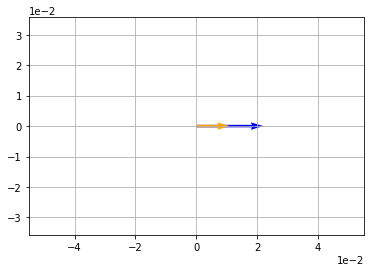
\includegraphics[width=0.5\linewidth,keepaspectratio]{vec7}
\end{center}
The original vector v is shown in orange, and the transformed vector t is shown in blue - note that t has the same direction (amplitude) as v but a greater length (magnitude).
 
\end{frame}


%%%%%%%%%%%%%%%%%%%%%%%%%%%%%%%%%%%%%%%%%%%%%%%%%%%%%%%%%%%
 \begin{frame}[fragile] \frametitle{Affine Transformations}
An Affine transformation multiplies a vector by a matrix and adds an offset vector, sometimes referred to as bias; like this:

\begin{itemize}

\item $T(\vec{v}) = A\vec{v} + \vec{b}$
\item $\begin{bmatrix}5 & 2\\3 & 1\end{bmatrix} \cdot  \begin{bmatrix}1\\1\end{bmatrix} + \begin{bmatrix}-2\\-6\end{bmatrix} = \begin{bmatrix}5\\-2\end{bmatrix}$
\end{itemize}

\end{frame}

%%%%%%%%%%%%%%%%%%%%%%%%%%%%%%%%%%%%%%%%%%%%%%%%%%%%%%%%%%%
 \begin{frame}[fragile] \frametitle{Affine Transformations}
\begin{lstlisting}
import numpy as np
import matplotlib.pyplot as plt
v = np.array([1,1])
A = np.array([[5,2],
              [3,1]])
b = np.array([-2,-6])

t = A@v + b
print (t)

# Plot v and t
vecs = np.array([v,t])
origin = [0], [0]
plt.axis('equal')
plt.grid()
plt.ticklabel_format(style='sci', axis='both', scilimits=(0,0))
plt.quiver(*origin, vecs[:,0], vecs[:,1], color=['orange', 'blue'], scale=15)
plt.show()
\end{lstlisting}
[ 5 -2]
\end{frame}

%%%%%%%%%%%%%%%%%%%%%%%%%%%%%%%%%%%%%%%%%%%%%%%%%%%%%%%%%%%
 \begin{frame}[fragile] \frametitle{Affine Transformations}


\begin{center}
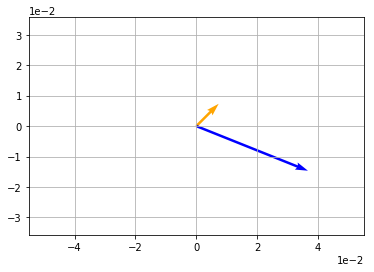
\includegraphics[width=0.5\linewidth,keepaspectratio]{vec8}
\end{center}
 
\end{frame}

%%%%%%%%%%%%%%%%%%%%%%%%%%%%%%%%%%%%%%%%%%%%%%%%%%%%%%%%%%%
 \begin{frame}[fragile] \frametitle{Meaning of Determinant}

\begin{itemize}

\item You could think of a determinant as a volume. Think of the columns of the matrix as vectors at the origin forming the edges of a skewed box. The determinant gives the volume of that box. For example, in 2 dimensions, the columns of the matrix are the edges of a rhombus.

\item If you consider the matrix as something that multiplies a vector and transforms it linearly to another vector, the determinant is the factor it increases the area/volume/hypervolume/etc of a parallelogram/parallelepiped/hyperparallepiped/etc built from a bunch of vectors.
 \end{itemize}

\end{frame}



%%%%%%%%%%%%%%%%%%%%%%%%%%%%%%%%%%%%%%%%%%%%%%%%%%%%%%%%%%%%%%%%%%%%%%%%%%%%%%%%%%
  \begin{frame}[fragile]\frametitle{}
\begin{center}
{\Large Eigenvectors}
\end{center}
\end{frame}

%%%%%%%%%%%%%%%%%%%%%%%%%%%%%%%%%%%%%%%%%%%%%%%%%%%%%%%%%%%
  \begin{frame}[fragile]{Eigenvectors}
\begin{itemize}

\item When you transform a vector using a matrix, we change its direction, length, or both. 
\item When the transformation only affects scale (in other words, the output vector has a different magnitude but the same amplitude as the input vector), the matrix multiplication for the transformation is the equivalent operation as some scalar multiplication of the vector.
\end{itemize}

\end{frame}

%%%%%%%%%%%%%%%%%%%%%%%%%%%%%%%%%%%%%%%%%%%%%%%%%%%%%%%%%%%
  \begin{frame}[fragile]{Eigenvectors}
\begin{itemize}

\item $\begin{bmatrix}2 & 0\\0 & 2\end{bmatrix} \cdot  \begin{bmatrix}1\\0\end{bmatrix} = \begin{bmatrix}2\\0\end{bmatrix}$
\item You can achieve the same result by mulitplying the vector by the scalar value 2:
\item $2 \times \begin{bmatrix}1\\0\end{bmatrix} = \begin{bmatrix}2\\0\end{bmatrix}$
\item The scalar-vector pairs that correspond to the matrix are known respectively as eigenvalues and eigenvectors. 
\end{itemize}

\end{frame}


%%%%%%%%%%%%%%%%%%%%%%%%%%%%%%%%%%%%%%%%%%%%%%%%%%%%%%%%%%%
  \begin{frame}[fragile]{Eigenvectors}
\begin{lstlisting}
import numpy as np
A = np.array([[2,0],
              [0,3]])
eVals, eVecs = np.linalg.eig(A)
print(eVals)
print(eVecs)
\end{lstlisting}
[2. 3.]
[[1. 0.]
 [0. 1.]]
\end{frame}

%%%%%%%%%%%%%%%%%%%%%%%%%%%%%%%%%%%%%%%%%%%%%%%%%%%%%%%%%%%
  \begin{frame}[fragile]{Eigenvectors}
\begin{itemize}

\item So there are two eigenvalue-eigenvector pairs for this matrix, as shown here:
\item $\lambda_{1} = 2, \vec{v_{1}} = \begin{bmatrix}1 \\ 0\end{bmatrix}  \;\;\;\;\;\; \lambda_{2} = 3, \vec{v_{2}} = \begin{bmatrix}0 \\ 1\end{bmatrix}$
\item Let's verify that multiplying each eigenvalue-eigenvector pair corresponds to the dot-product of the eigenvector and the matrix. Here's the first pair:
\item $2 \times \begin{bmatrix}1 \\ 0\end{bmatrix} = \begin{bmatrix}2 \\ 0\end{bmatrix}  \;\;\;and\;\;\; \begin{bmatrix}2 & 0\\0 & 3\end{bmatrix} \cdot \begin{bmatrix}1 \\ 0\end{bmatrix} = \begin{bmatrix}2 \\ 0\end{bmatrix}$
\item So far so good. Now let's check the second pair: $3 \times \begin{bmatrix}0 \\ 1\end{bmatrix} = \begin{bmatrix}0 \\ 3\end{bmatrix}  \;\;\;and\;\;\; \begin{bmatrix}2 & 0\\0 & 3\end{bmatrix} \cdot \begin{bmatrix}0 \\ 1\end{bmatrix} = \begin{bmatrix}0 \\ 3\end{bmatrix}$
\item So our eigenvalue-eigenvector scalar multiplications do indeed correspond to our matrix-eigenvector dot-product transformations.
\end{itemize}

\end{frame}





%%%%%%%%%%%%%%%%%%%%%%%%%%%%%%%%%%%%%%%%%%%%%%%%%%%%%%%%%%%%%%%%%%%%%%%%%%%%%%%%%%
  \begin{frame}[fragile]{Eigenvectors}
 \textbf{Definition}
 Let $A$ be an $n \times n$ matrix.  A {\em non-zero} vector $\vec{x}\in \mathbb R^n$ is 
called an \textbf{eigenvector} of $A$ if there exists some scalar $\lambda \in \mathbb R$ so that 
$A \vec{x}= \lambda \vec{x}$.  \\ 
 If $\vec{x}$ is an eigenvector of $A$,
the corresponding value $\lambda$ is called an \textbf{eigenvalue} of $A$, and we say that 
$\lambda$ is an eigenvalue of $A$ with eigenvector $\vec{x}$.  



\textbf{Note}
While an eigenvector $\vec{x}$ must be non-zero (so that we are always 
excluding the trivial case $A \vec{0}=\vec{0}$), it is possible for the value
$\lambda$ to be zero. 



\textbf{Example}
$\left[ \begin{array}{rrrrr} 1 & 2 \\ 2 & 4 \end{array} \right]$
has eigenvector $\left[ \begin{array}{rrrrr}2 \\-1 \end{array} \right]$ with eigenvalue $0$.

\end{frame}




%%%%%%%%%%%%%%%%%%%%%%%%%%%%%%%%%%%%%%%%%%%%%%%%%%%%%%%%%%%%%%%%%%%%%%%%%%%%%%%%%%
  \begin{frame}[fragile]
\textbf{Note}
 If $\lambda$ is an eigenvalue for $A$, the eigenvectors for $A$ corresponding to $\lambda$ along with $\vec{0}$ form a subspace of $\mathbb R^n$.



 \textbf{Example}
 \[
 \left[ \begin{array}{rrrrr} 
  1 & 6 \\ 5 & 2
 \end{array} \right]
 \left[ \begin{array}{rrrrr} 
  6 \\-5 
 \end{array} \right]
=
 \left[ \begin{array}{rrrrr} 
  -24 \\ 20
 \end{array} \right]
=
-4 \left[ \begin{array}{rrrrr} 
  6 \\ -5
 \end{array} \right].
\]


Thus we see that $\left[ \begin{array}{rrrrr} 
  6 \\ -5
 \end{array} \right]$ is an eigenvector of this matrix, and $-4$ is the corresponding eigenvalue.

 
\end{frame}



%%%%%%%%%%%%%%%%%%%%%%%%%%%%%%%%%%%%%%%%%%%%%%%%%%%%%%%%%%%%%%%%%%%%%%%%%%%%%%%%%%
  \begin{frame}[fragile]
\textbf{Example}
 Show that 7 is an eigenvalue for 
 \[
 A = \left[ \begin{array}{rrrrr} 2 & 4 \\ 5 & 3 \end{array} \right].
\]



\textbf{Note}
For any scalar $\lambda$,
\begin{eqnarray*}
 A \vec{x} &=& \lambda \vec{x}   \\
 &\Leftrightarrow&  
A \vec{x} -\lambda \vec{x} = \vec{0}  \\
 &\Leftrightarrow&  
 A \vec{x} -\lambda I \vec{x} = \vec{0}  \\
  &\Leftrightarrow& 
  \left[ A - \lambda I \right] \vec{x} =\vec{0} \\
   &\Leftrightarrow&  
\vec{x} \in \ Nul(A -\lambda I)
\end{eqnarray*}

\end{frame}




%%%%%%%%%%%%%%%%%%%%%%%%%%%%%%%%%%%%%%%%%%%%%%%%%%%%%%%%%%%%%%%%%%%%%%%%%%%%%%%%%%
  \begin{frame}[fragile]
\textbf{Definition}
 If $\dim(Nul(A - \lambda I))>0$, then $Nul(A-\lambda I)$ is called the \textbf{eigenspace } for 
$A$ corresponding to the eigenvalue $\lambda$, since any 
$\vec{x}\in Nul(A-\lambda I) $ satisfies $A\vec{x} =  \lambda \vec{x}$.



\textbf{Example}
 Find a basis for the eigenspace corresponding to the eigenvector $2$ for the 
matrix
\[
 A = \left[ \begin{array}{rrrrr}
      4 & -1 & 6 \\
      2 & 1 & 6 \\
      2 & -1 & 8 
     \end{array} \right].
\]

\end{frame}




%%%%%%%%%%%%%%%%%%%%%%%%%%%%%%%%%%%%%%%%%%%%%%%%%%%%%%%%%%%%%%%%%%%%%%%%%%%%%%%%%%
  \begin{frame}[fragile]
 \textbf{Theorem}
 The eigenvalues of an upper triangular matrix (or of a lower triangular matrix) are its
diagonal entries. 



\textbf{Invertible Matrix Theorem}
 \begin{itemize}
 \item[] The number 0 is an eigenvalue of $A$   
\item[] $\iff$  there exists $\vec{x} \neq \vec{0}$ so that 
$A \vec{x} = 0 \vec{x}$  
\item[] $\iff$   there exists $\vec{x} \neq \vec{0}$ so that 
$A \vec{x} - 0 \vec{x} = \vec{0}$.
\item[] $\iff$  There exists $\vec{x} \neq \vec{0} \in \text{Nul}(A)$.
\item[] $\iff$  $A$ is not invertible. 
\end{itemize}



\textbf{Theorem}
 If $\vec{v}_1, \dots, \vec{v}_r$ are eigenvectors corresponding to 
distinct eigenvalues $\lambda_1, \dots, \lambda_r$ of an $n\times n$ matrix $A$,
then the set $\{\vec{v}_1, \dots,\vec{v}_r\}$ is linearly independent.

\end{frame}




%%%%%%%%%%%%%%%%%%%%%%%%%%%%%%%%%%%%%%%%%%%%%%%%%%%%%%%%%%%%%%%%%%%%%%%%%%%%%%%%%%
  \begin{frame}[fragile]
\textbf{Example}
In many applications, one is interested in studying repeated application of a linear map.  \\ 
Suppose we would like to study the long term behavior of a sequence $\{\vec{x}_k\}$ satisfying $\vec{x}_{k+1}=A\vec{x}_k$. \\ 
Describe the long term behavior of such a sequence where $\vec{x}_0$ is an eigenvector of $A$ with eigenvalue $\lambda$. \\ 

\end{frame}


%%%%%%%%%%%%%%%%%%%%%%%%%%%%%%%%%%%%%%%%%%%%%%%%%%%%%%%%%%%
\begin{frame}[fragile]\frametitle{Note}

To find the eigenvalues of a matrix $A$, we must determine values $\lambda\in  \mathbb R$ such that $Nul(A-\lambda I)\neq\{\vec{0}\}$.  \\
Recall that this is equivalent to $A-\lambda I$ being singular  or $\det(A-\lambda I)=0$.

\textbf{Example}
Find the eigenvalues of 
$A = \left[ \begin{array}{rrrrr} 3 & -2 \\ 1 & 0 \end{array} \right]$
\end{frame}

%%%%%%%%%%%%%%%%%%%%%%%%%%%%%%%%%%%%%%%%%%%%%%%%%%%%%%%%%%%
\begin{frame}[fragile]\frametitle{Facts}

For a general $2\times 2$ matrix $\left[ \begin{array}{rrrrr} a & b \\ c & d \end{array} \right]$, 
the formula for the determinant enables us to compute the eigenvalues easily.
\begin{eqnarray*}
\det (A-\lambda I) &=&  
 \det \left[ \begin{array}{cc} (a-\lambda) & b \\ c & (d-\lambda) \end{array} \right]  \\
&=&    (a-\lambda)(d-\lambda) -bc  \\ &=& \lambda^2 - (a+d)\lambda + (ad-bc).
\end{eqnarray*}  
So that the quadratic formula gives   
\[
 \lambda = \frac{(a+d) \pm \sqrt{(a+d)^2 -4(ad-bc)} }{2}.
\]

\end{frame}

%%%%%%%%%%%%%%%%%%%%%%%%%%%%%%%%%%%%%%%%%%%%%%%%%%%%%%%%%%%
\begin{frame}[fragile]\frametitle{Advanced Example}

Let  $A = \left[ \begin{array}{rrrrr} \cos \theta & -\sin \theta \\ \sin \theta & \cos \theta \end{array} \right]$
be the matrix which rotates a vector counter clockwise through an angle $\theta$.  Then we have
\[
 \det(A-\lambda I) = \lambda^2 - 2 \lambda \cos \theta + 1.
\]
So $\lambda = \cos \theta \pm \sqrt{cos^2\theta-1} = \cos \theta \pm i \sin\theta = e^{\pm i\theta}$, where
$i = \sqrt{-1}$.  So unless $\sin \theta =0$, there are no real eigenvalues.


\end{frame}

% %%%%%%%%%%%%%%%%%%%%%%%%%%%%%%%%%%%%%%%%%%%%%%%%%%%%%%%%%%%
% \begin{frame}[fragile]\frametitle{Example}

% \textbf{Theorem}[The Invertible Matrix Theorem continued]
% Let $A$ be an $n\times n$ matrix.  Then $A$ is invertible if and only if 
% \begin{itemize}
 % \item[(s)] The number 0 is {\em not} an eigenvalue of $A$.
% \item[(t)] The determinant of $A$ is not zero.
% \end{itemize}
  
% \end{frame}


  % \begin{frame}[fragile]
% \textbf{Theorem}[Properties of Determinants]
% Let $A$ and $B$ be $n\times n$ matrices.
 % \begin{itemize}
  % \item $A$ is invertible if and only if $\det(A)\neq 0$
% \item[(b)] $\det(AB)=\det(A)\det(B)$.
% \item[(c)] $\det(A^T)= \det(A)$.
% \item[(d)] If $A$ is triangular, then $\det(A)$ is the product of the entries on
% the main diagonal.
% \item[(e)] A row replacement operation on $A$ doesn't change the determinant.   A row interchange
% switches the sign of the determinant.  A row scaling also scales the determinant by the same 
% scale factor.   
 % \end{itemize}

% \end{frame}


%%%%%%%%%%%%%%%%%%%%%%%%%%%%%%%%%%%%%%%%%%%%%%%%%%%%%%%%%%%
\begin{frame}[fragile]\frametitle{Theorem}

 A scalar $\lambda$ is an eigenvalue of an $n\times n$ matrix $A$ if and only if 
$\lambda$ satisfies the \textbf{characteristic equation} 
\[
 \det(A -\lambda I) = 0.
\]

\textbf{Facts}
$\det(A-\lambda I)$ is a polynomial in $\lambda$ of degree $n$.   \\ 
Hence, an $n\times n$ matrix has at most $n$ eigenvalues. 

\end{frame}


%%%%%%%%%%%%%%%%%%%%%%%%%%%%%%%%%%%%%%%%%%%%%%%%%%%%%%%%%%%
\begin{frame}[fragile]\frametitle{Definition}

\begin{itemize}
\item  The degree $n$ polynomial $\det(A-\lambda I)$ is called the \textbf{characteristic polynomial}.  
\item  The \textbf{(algebraic) multiplicity} of the eigenvalue $\lambda_0$ is the power of $(\lambda-\lambda_0)$ appearing in the factorization of the characteristic polynomial.
\end{itemize}

\textbf{Example}
Find the eigenvalues and their multiplicities of 
\[A = \left[ \begin{array}{rrrrr} 
 6 & 5 & 0 & -5 \\ 0 & -3 & 1 & 2 \\ 0 & 0 & 6 & 3 \\ 0& 0 & 0 & 7     
     \end{array} \right].
\]

\end{frame}
% %%%%%%%%%%%%%%%%%%%%%%%%%%%%%%%%%%%%%%%%%%%%%%%%%%%%%%%%%%%%%%%%%%%%%%%%%%%%%%%%%%
  \begin{frame}[fragile]\frametitle{}
\begin{center}
{\Large Linear Equations }
\end{center}
\end{frame}


%%%%%%%%%%%%%%%%%%%%%%%%%%%%%%%%%%%%%%%%%%%%%%%%%%%%%%%%%%%
  \begin{frame}[fragile]\frametitle{Linear Equations}

Consider the simultaneous equations
\begin{eqnarray*}
x + 2y &=& 4\\
3x-5y &=& 1 
\end{eqnarray*}
Provided you understand how matrices are multiplied together you will realize
that these can be written in matrix form as
$$
\left[
\begin{array}{cc}
1 & 2 \\
3 & -5 \\
\end{array}
\right]\left[
\begin{array}{c}
x \\
y\\
\end{array}\right] =\left[
\begin{array}{c}
4 \\
1\\
\end{array} 
\right]
$$
Writing
$$
A = \left[
\begin{array}{cc}
1 & 2 \\
3 & -5 \\
\end{array}
\right], X = \left[
\begin{array}{c}
x \\
y\\
\end{array}\right], \hbox { and } B=\left[
\begin{array}{c}
4 \\
1\\
\end{array} 
\right]
$$
we have
$$
AX=B
$$
\end{frame}


%%%%%%%%%%%%%%%%%%%%%%%%%%%%%%%%%%%%%%%%%%%%%%%%%%%%%%%%%%%
  \begin{frame}[fragile]\frametitle{Linear Equations}

We need to calculate the inverse of $A=\left[
\begin{array}{cc}
1 & 2 \\
3 & -5 \\
\end{array}
\right]$.

\begin{eqnarray*}
A^{-1} &=& \frac{1}{(1)(-5)-(2)(3)}\left[
\begin{array}{cc}
-5 & -2 \\
-3 & 1 \\
\end{array}
\right] \\
&=& -\frac{1}{11}\left[
\begin{array}{cc}
-5 & -2 \\
-3 & 1 \\
\end{array}
\right] 
\end{eqnarray*}
Then $X$ is given by
\begin{eqnarray*}
X = A^{-1}B &=&-\frac{1}{11}\left[
\begin{array}{cc}
-5 & -2 \\
-3 & 1 \\
\end{array}
\right]  \left[
\begin{array}{c}
4 \\
1\\
\end{array} 
\right] \\
&=& -\frac{1}{11}\left[
\begin{array}{c}
-22\\
-11\\
\end{array} 
\right]
= \left[
\begin{array}{c}
2\\
1\\
\end{array} 
\right]
\end{eqnarray*}
Hence $x=2$, $y=1$ is the solution of the simultaneous equations.

\end{frame}

%%%%%%%%%%%%%%%%%%%%%%%%%%%%%%%%%%%%%%%%%%%%%%%%%%%%%%%%%%%
  \begin{frame}[fragile]\frametitle{Linear Equations}
$m$ linear equations of $n$ variables.

$a_{11} x_1 + a_{12}x_2 + \ldots + a_{1n} = u_1$\\
$a_{21} x_1 + a_{22}x_2 + \ldots + a_{2n} = u_2$\\
\ldots \\
$a_{m1} x_1 + a_{m2}x_2 + \ldots + a_{mn} = u_m$ \\

Can be written in matrix form as :

$$ \left[ \begin{array}{ccc} a_{11} \hspace{1mm} a_{12} \hspace{1mm}
                                    \ldots \hspace{1mm} a_{1n} \\
                              a_{21} \hspace{1mm} a_{22} \hspace{1mm} 
                                     \ldots \hspace{1mm} a_{2n} \\
                              \vdots \hspace{6mm} \vdots \hspace{11mm} \vdots \\
                              a_{m1} \hspace{1mm} a_{m2} \hspace{1mm}
                                     \ldots \hspace{1mm} a_{mn}
              \end{array}  \right]   \left[ \begin{array}{c} x_{1} \\ x_2 \\ \vdots \\ x_m               \end{array}  \right] 
                =  \left[ \begin{array}{c} u_{1} \\ u_2 \\ \vdots \\ u_m               \end{array}  \right]                $$
\end{frame}

%%%%%%%%%%%%%%%%%%%%%%%%%%%%%%%%%%%%%%%%%%%%%%%%%%%%%%%%%%%
  \begin{frame}[fragile]\frametitle{Example}
\begin{itemize}
\item $x$: price of pencil
\item $y$: price of pen
\item $u$: box 1
\item $v$: box 2
\item Set I: \begin{align} 2x + 3y = u \\ 3x+4y = v\end{align}
\item Set II: \begin{align} 2u + v = 57 \\ 3u+2v = 97\end{align}
\end{itemize}
\end{frame}

%%%%%%%%%%%%%%%%%%%%%%%%%%%%%%%%%%%%%%%%%%%%%%%%%%%%%%%%%%%
  \begin{frame}[fragile]\frametitle{Example}
II by putting $u,v$ from I

\begin{align} 2(2x + 3y) + 1(3x+4y) = 57 \\  3(2x + 3y) + 2(3x+4y) = 97\end{align}
Collecting $x,y$
\begin{align} [(2x2) + (3x1)]x + [(2x3) + (4x1)]y = 57 \\   [(2x2) + (3x1)]x + [(2x3) + (4x1)]y = 97\end{align}

$$
\left[
\begin{array}{cc}
2 & 1 \\
3 & 2 \\
\end{array}
\right]
\left[
\begin{array}{cc}
2 & 3 \\
3 & 4 \\
\end{array}
\right]\left[
\begin{array}{c}
x \\
y\\
\end{array}\right] =\left[
\begin{array}{c}
57 \\
97\\
\end{array} 
\right]
$$
\end{frame}


%%%%%%%%%%%%%%%%%%%%%%%%%%%%%%%%%%%%%%%%%%%%%%%%%%%%%%%%%%%
  \begin{frame}[fragile]\frametitle{Solving Simultaneous Equations}
$$ \left[ \begin{array}{ccc} a_1 \hspace{1mm} a_2 \hspace{1mm} \hspace{1mm} a_3 \\
                              a_4 \hspace{1mm} a_5 \hspace{1mm} \hspace{1mm} a_6 \\
                             a_7 \hspace{1mm} a_8 \hspace{1mm} \hspace{1mm} a_9\end{array}  \right]   
                             \left[ \begin{array}{c} x \\ y\\z\end{array}  \right] 
                =  \left[ \begin{array}{c} c_1\\ c_2  \\ c_3              \end{array}  \right]                $$
                
Make augmented matrix
$$ \left[ \begin{array}{cccc} a_1 \hspace{1mm} a_2 \hspace{1mm} \hspace{1mm} a_3  \hspace{1mm} |c_1\\
                              a_4 \hspace{1mm} a_5 \hspace{1mm} \hspace{1mm} a_6  \hspace{1mm} |c_2 \\
                             a_7 \hspace{1mm} a_8 \hspace{1mm} \hspace{1mm} a_9  \hspace{1mm} |c_3 \end{array}  \right]   $$

Row operations permitted
\begin{itemize}
\item Interchange of rows
\item Multiply by scalar
\item Add rows
\end{itemize}     
Using this make lower triable 0, and get the answers.           
\end{frame}

%%%%%%%%%%%%%%%%%%%%%%%%%%%%%%%%%%%%%%%%%%%%%%%%%%%%%%%%%%%
  \begin{frame}[fragile]\frametitle{Assignment}
\begin{itemize}
\item Q: Similar to row transformations can we apply column transformations as well? Difference?
\item A: We can use column transformations as well but in that case the $x$ vector changes. Eg. In case of $C_1 \Longleftrightarrow C_3$, $\left[
\begin{array}{c}
x_3 \\ x_2\\ x_1
\end{array} 
\right]$ is the $x$ vector.
\end{itemize}
\end{frame}

%%%%%%%%%%%%%%%%%%%%%%%%%%%%%%%%%%%%%%%%%%%%%%%%%%%%%%%%%%%
  \begin{frame}[fragile]\frametitle{}
A system of linear equations is a collection of equations in the same set of variables. 

 For example,
\begin{equation*}
\begin{cases}
 x_1 + 3 x_2 &=5\\
 2x_1 -x_2 &= -4
\end{cases}
\end{equation*}

\begin{itemize}
\item Pair of equations in two variables
\item Think of this as the intersection of two lines.
 \item Sketch these lines and find their intersection.
\end{itemize}
\end{frame}

%%%%%%%%%%%%%%%%%%%%%%%%%%%%%%%%%%%%%%%%%%%%%%%%%%%%%%%%%%%
  \begin{frame}[fragile] \frametitle{Solution Sets} 
The solution set for a linear system of equations can be:

\begin{itemize}
 \item Empty. (there is no solution.)
 \item Exactly one solution
 \item More than one solution
\end{itemize}

\end{frame}

%%%%%%%%%%%%%%%%%%%%%%%%%%%%%%%%%%%%%%%%%%%%%%%%%%%%%%%%%%%
  \begin{frame}[fragile] \frametitle{Solution Sets} 
\begin{itemize}
 \item It is easy to come up with examples of the first two circumstances.  
 \item The third possibility actually means that something much stronger is true.
\item If we have two distinct solutions then we must have infinitely many solutions.
\item Why is it that if we have at least two solutions then there are infinitely many?
\end{itemize}

\textbf {To Do}
Draw two dimensional examples illustrating each of the three possible outcomes. 


\end{frame}




%%%%%%%%%%%%%%%%%%%%%%%%%%%%%%%%%%%%%%%%%%%%%%%%%%%%%%%%%%%
  \begin{frame}[fragile]  \frametitle{Matrix Notation}
The system of equations above has coefficient matrix
$$
\begin{bmatrix}
 1 & 3 \\
 2 & -1
\end{bmatrix}
$$


and augmented matrix 
$$
\begin{bmatrix}
 1 & 3 & 5\\
 2 & -1 & -4
\end{bmatrix}
$$

\end{frame}




%%%%%%%%%%%%%%%%%%%%%%%%%%%%%%%%%%%%%%%%%%%%%%%%%%%%%%%%%%%
  \begin{frame}[fragile]\frametitle{Elementary row operations}

\textbf {To Do}
 Subtract twice the first row from the second row of the augmented matrix.
 Explain why the new system of equations has precisely the same set of solutions
 as the old set of equations.



\textbf{Operations}
here are 3 types of elementary row operations.
\begin{itemize}
 \item (Replacement) Replace a row by the sum of {\em the same row} and a multiple of {\em different} row. 
 \item (Interchange)  Interchange two rows.
 \item (Scaling) Multiply a row by a non-zero constant.
\end{itemize}


\end{frame}


%%%%%%%%%%%%%%%%%%%%%%%%%%%%%%%%%%%%%%%%%%%%%%%%%%%%%%%%%%%
  \begin{frame}[fragile]\frametitle{}
\textbf{Notation}
\begin{itemize}
\item (Replacement) The operation of replacing row $i$ by itself plus  $c$ times row $j$ will be denoted $R_i + cR_j$.
\item (Interchange)  The operation of interchanging rows $i$ and $j$ will be denoted by $R_i \leftrightarrow R_j$.
\item (Scaling) The operation of scaling row $i$ by a nonzero constant $c$ will be denoted by $cR_i$.
\end{itemize}


\end{frame}


%%%%%%%%%%%%%%%%%%%%%%%%%%%%%%%%%%%%%%%%%%%%%%%%%%%%%%%%%%%
  \begin{frame}[fragile]\frametitle{}

It is clear that the set of solutions is not changed by the second and third operations.  



\textbf{To Do}
 Explain why the set of solutions is unchanged by the first operation.



\end{frame}

%%%%%%%%%%%%%%%%%%%%%%%%%%%%%%%%%%%%%%%%%%%%%%%%%%%%%%%%%%%
  \begin{frame}[fragile]\frametitle{Equivalence of Linear Systems}
\textbf{Definition}
\begin{itemize}
 \item Two linear systems are \textbf{equivalent} if they have the same solution set.
 \item Two matrices are \textbf{row equivalent} if one matrix can be obtained from the other
 by elementary row operations.
\end{itemize}



\textbf{Principle}  Suppose $A$ and $B$ are $m \times n$ matrices: explain why the following 
 is true: if $A$ can be reduced via elementary row operations to $B$, then $B$ can be reduced
 to $A$. 
 



The key fact to notice is that these operations can be undone or inverted.

\end{frame}

%%%%%%%%%%%%%%%%%%%%%%%%%%%%%%%%%%%%%%%%%%%%%%%%%%%%%%%%%%%
  \begin{frame}[fragile]\frametitle{}
Two linear systems are equivalent if and only if their augmented matrices
are row-equivalent.



 Write the following system of equations as an augmented matrix and solve the system:
 \[
\begin{array}{rcrcrcr}
  x_1  & + &       & + & -3 x_3 & =  & 8 \\
  2x_1 & + & 2 x_2 & + & 9 x_3  & =  & 7 \\
       & + &  x_2  & + & 5 x_3  & =  & -2 
\end{array}
\]

\end{frame}


%%%%%%%%%%%%%%%%%%%%%%%%%%%%%%%%%%%%%%%%%%%%%%%%%%%%%%%%%%%
  \begin{frame}[fragile]\frametitle{Fundamental Questions}

We can rephrase our question about how many solutions there are to a system in the following way.


\begin{itemize}
 \item Is the system consistent, that is, do there exist {\em any} solutions?
 \item If there is at least one solution, is it unique?
\end{itemize}

\end{frame}

%%%%%%%%%%%%%%%%%%%%%%%%%%%%%%%%%%%%%%%%%%%%%%%%%%%%%%%%%
  \begin{frame}[fragile]\frametitle{Fundamental Questions}

For example, we've seen that the system 
\begin{eqnarray*}
 x_1 + 3 x_2 &=&5\\
 2x_1 -x_2 &=& -4
\end{eqnarray*}
has a unique solution. 
On the other hand, the system 
\begin{eqnarray*}
 x_1 + 3 x_2 &=&5\\
 2x_1 +6 x_2 &=& -4
\end{eqnarray*}
has no solutions,
 and the system
\begin{eqnarray*}
 x_1 + 3 x_2 &=&5\\
 2x_1 +6 x_2 &=& 10
\end{eqnarray*}
has infinitely many.

\end{frame}

%%%%%%%%%%%%%%%%%%%%%%%%%%%%%%%%%%%%%%%%%%%%%%%%%%%%%%%%%%%
  \begin{frame}[fragile]\frametitle{Row Reduction and Row Echelon Form}
 A rectangular matrix is in \textbf{echelon form}
(or \textbf{row echelon form}) if it has the following properties
\begin{itemize}
 \item All non-zero rows are above any rows of all zeros.
 \item Each leading entry of a row is in a column to the right of the leading
 entry of the row above it.
 \item All entries in a column below a leading entry are zeros.
\end{itemize}

\end{frame}

%%%%%%%%%%%%%%%%%%%%%%%%%%%%%%%%%%%%%%%%%%%%%%%%%%%%%%%%%%%
  \begin{frame}[fragile]\frametitle{Row Reduction and Row Echelon Form}
\begin{itemize}
 \item Sometimes we want more than echelon form. 
 \item  We can make all the leading 
entries 1 by multiplying by a constant, and we can subtract from rows 
above to zero out their entries in that column.
\end{itemize}

\textbf{Definition} A rectangular matrix is in \textbf{reduced echelon form}
(or \textbf{reduced row echelon form}) if it is in row echelon form, and 
 has the following additional properties
\begin{itemize}
 \item The leading non-zero term of every non-zero row is 1
 \item Each leading 1 is the only non-zero entry in its column.
\end{itemize}

\end{frame}

%%%%%%%%%%%%%%%%%%%%%%%%%%%%%%%%%%%%%%%%%%%%%%%%%%%%%%%%%%%
  \begin{frame}[fragile]\frametitle{Row Reduction and Row Echelon Form}
\noindent{\bf Examples} 
\[
\begin{bmatrix}
 1 & 2 & 5 \\
 0 & 2 & 6 \\
 0 & 0 & 0
\end{bmatrix}
\]

is in row echelon form but is not reduced:
\[
\begin{bmatrix}
 1 & 2 & 5 \\
 0 & 1 & 3 \\
 0 & 0 & 0
\end{bmatrix}
\] 
is in row echelon form but is not reduced:
\end{frame}

%%%%%%%%%%%%%%%%%%%%%%%%%%%%%%%%%%%%%%%%%%%%%%%%%%%%%%%%%%%
  \begin{frame}[fragile]\frametitle{Row Reduction and Row Echelon Form}
\noindent{\bf Examples} 
\[
\begin{bmatrix}
 1 & 0 & -1 \\
 0 & 1 & 3 \\
 0 & 0 & 0
\end{bmatrix}
\] 
is in reduced row echelon form:
\[
\begin{bmatrix}
 1 & 2 & 5 \\
 0 & 1 & 3 \\
 2 & 0 & 0
\end{bmatrix}
\] 
is not in row echelon form.
\end{frame}

%%%%%%%%%%%%%%%%%%%%%%%%%%%%%%%%%%%%%%%%%%%%%%%%%%%%%%%%%%%
  \begin{frame}[fragile]\frametitle{Row Reduction and Row Echelon Form}

\textbf{Solving a system in reduced row echelon form}
Suppose we have a system of equations, we've written them as an 
augmented matrix, we've performed elementary row operations, and arrived
at the following reduced row echelon form matrix.  
\[
 \begin{bmatrix}
  1 & 6 & 0 & 3 & 0 & 0 \\
  0 & 0 & 1 & -4 & 0 & 5\\
  0 & 0 & 0 & 0 & 1 & 7 
 \end{bmatrix}
 \]
 
 
\begin{itemize}
 \item  Write down the corresponding equations.
 \item  Pair up the variables and the pivot columns: these are the \textbf{basic variables}.
 \item  The remaining variables are the \textbf{free variables}.
\end{itemize}

\end{frame}

%%%%%%%%%%%%%%%%%%%%%%%%%%%%%%%%%%%%%%%%%%%%%%%%%%%%%%%%%%%
  \begin{frame}[fragile]\frametitle{Great News}

\begin{itemize}
 \item  Each matrix is row equivalent to one and only one reduced echelon matrix.
\item Gaussian elimination: How do we get a matrix into row echelon or reduced row echelon form?
\end{itemize}
\end{frame}

%%%%%%%%%%%%%%%%%%%%%%%%%%%%%%%%%%%%%%%%%%%%%%%%%%%%%%%%%%%
  \begin{frame}[fragile]{Gaussian Elimination}
\begin{itemize} 
\item We start with the left-most
non-zero column,
\item Working to the right and from the top down.  
\item At 
each stage, we will be working with the portion of the matrix which 
is below or to the right (or both) of the pivot.
\end{itemize}
\end{frame}

%%%%%%%%%%%%%%%%%%%%%%%%%%%%%%%%%%%%%%%%%%%%%%%%%%%%%%%%%%%
  \begin{frame}[fragile]{Gaussian Elimination}
\begin{itemize} 
\item Find the left-most column containing a non-zero entry.  This is 
a pivot column: the pivot position is at the top.   
\item Select a non-zero entry in the column to be the pivot. By 
interchanging rows if necessary, move the pivot into the pivot position.  
\item Use row replacement operations to change all the values below the pivot
to zero.  
\item Move to the next row, and apply steps 1, 2, 3 to the remaining
submatrix, namely the rows below and including the current row.
\end{itemize}

Once we've gone through all the rows, the matrix is in row echelon form.
\end{frame}

%%%%%%%%%%%%%%%%%%%%%%%%%%%%%%%%%%%%%%%%%%%%%%%%%%%%%%%%%%%

  \begin{frame}[fragile]\frametitle{Gaussian Elimination}

\begin{itemize}   
\item Scale pivots to be 1 
\item Use row replacement operations to change all the values above 
pivots to be zero.  (There are technical reasons for doing this from the 
bottom pivot first).
\end{itemize}
\end{frame}



%%%%%%%%%%%%%%%%%%%%%%%%%%%%%%%%%%%%%%%%%%%%%%%%%%%%%%%%%%%
  \begin{frame}[fragile]\frametitle{Gaussian Elimination}

In order to obtain row echelon form, we only need to switch rows and subtract 
multiples below.

This process is often referred to as Gaussian elimination, or 
Gauss-Jordan elimination

\end{frame}


%%%%%%%%%%%%%%%%%%%%%%%%%%%%%%%%%%%%%%%%%%%%%%%%%%%%%%%%%%%
  \begin{frame}[fragile]\frametitle{Example}

 Row reduce 
 \begin{equation*}
   \begin{bmatrix}
   1& 3 & 5 & 7 \\
   3 & 5 & 7 & 9 \\
   5& 7 & 9 & 1
  \end{bmatrix}
  \rightarrow  \cdots
 \end{equation*}

\end{frame}

%%%%%%%%%%%%%%%%%%%%%%%%%%%%%%%%%%%%%%%%%%%%%%%%%%%%%%%%%%%
  \begin{frame}[fragile]\frametitle{Solutions of Linear Equations}
Recall that there are three possible outcomes:  
\begin{itemize}
 \item No solutions: for example
 \[
  \begin{bmatrix}
   1 & 0 & 0 & 5 \\
   0 & 1 & 1 & 3 \\
   0 & 0 & 0 & 6
  \end{bmatrix}
 \]


\item Unique solution: for example
\[
  \left[\begin{array}{rrrr}
   1 & 0 & 0 & -5 \\
   0 & 1 & 0 & 2 \\
   0 & 0 & 1 & 6
  \end{array}\right]
 \]
 
 \item Infinitely many solutions: for example
 \[
  \begin{bmatrix}
   1 & 2 & 0 & 6 \\
   0 & 0 & 1 & 3 \\
   0 & 0 & 0 & 0
  \end{bmatrix}
 \]
 \end{itemize}
 \end{frame}
 
 %%%%%%%%%%%%%%%%%%%%%%%%%%%%%%%%%%%%%%%%%%%%%%%%%%%%%%%%%%%
  \begin{frame}[fragile]\frametitle{General Form}
 In the last case, we write the solution set as 
 \[
  \left\{ 
  \begin{array}{rl}
   x_1 & =  6-2x_2 \\
   x_2 &  \mbox{is free}\\
   x_3 & =  3
  \end{array}
  \right.
 \]

\begin{itemize} 
\item This is called a {\em general solution}.
\item  $x_1$ and $x_3$ are called dependent variables.
\item $x_2$ is called a parameter or free variable or an independent variable.
\end{itemize}

\end{frame}

%%%%%%%%%%%%%%%%%%%%%%%%%%%%%%%%%%%%%%%%%%%%%%%%%%%%%%%%%%%
  \begin{frame}[fragile]
 Find the general solution to the linear system with augmented matrix
 \begin{equation*}
   \left[\begin{array}{rrrrrr}
   1 & 6 & 2 & -5 & -1 & -4 \\
   0 & 0 & 2 & -8 & -1 & 3 \\
   0 & 0 & 0 & 0  & 1  & 7
  \end{array}\right]
  \rightarrow \cdots
 \end{equation*}

\end{frame}


%%%%%%%%%%%%%%%%%%%%%%%%%%%%%%%%%%%%%%%%%%%%%%%%%%%%%%%%%%%
  \begin{frame}[fragile]
If a linear system is consistent then the solution set contains
either  
\begin{itemize}
\item A single element (-i.e. the solution is unique, there are no free variables).  
\item Infinitely many elements (-i.e. at least one free variable).
\end{itemize}
\end{frame}



%%%%%%%%%%%%%%%%%%%%%%%%%%%%%%%%%%%%%%%%%%%%%%%%%%%%%%%%%%%
  \begin{frame}[fragile]

\textbf{Solution Procedures} 
Given a linear system to solve
\begin{itemize}
 \item Write the augmented matrix   
 \item Perform row reduction to obtain echelon form.  If the system is not consistent then there are no solutions and you may stop. 
 \item Perform row reduction to obtain reduced echelon form.  
 \item Write system of equations corresponding to reduced echelon form.  
 \item Basic variables correspond to columns with pivots.  Free variables correspond to
 columns without pivots.  
 \item Write basic variables in terms of free variables.
\end{itemize}

\end{frame}


%%%%%%%%%%%%%%%%%%%%%%%%%%%%%%%%%%%%%%%%%%%%%%%%%%%%%%%%%%%
  \begin{frame}[fragile]
\textbf{Definition}
 If $A$ is an $m \times n$ matrix with columns 
 $\vec{a}_1, \vec{a}_2, \dots ,\vec{a}_n$,
and $\vec{x} \in \mathbb R^n$, then the product of $A$ and $\vec{x}$, 
which we denote by $A\vec{x}$, is defined to be 
\[ 
 A \vec{x} = 
 \left[\begin{array}{cccc}
  | & | & \dots & | \\
  \vec{a}_1 & \vec{a}_2 & \dots & \vec{a}_n  \\
  | & | & \dots & | \\
 \end{array}\right]
\left[\begin{array}{r} 
 x_1 \\ x_2 \\ \vdots \\ x_n
\end{array}\right]
\]
\[
 = x_1 \vec{a}_1 + x_2 \vec{a}_2 + \dots + x_n \vec{a}_n
\]


\textbf{Note}
\begin{itemize}
\item $A\vec{x} \in \mathbb R^m$.
\item $A\vec{x}$ is the linear combination of the columns of $A$ with weights $x_1, x_2, \dots, x_n$.
\end{itemize}

\end{frame}

%%%%%%%%%%%%%%%%%%%%%%%%%%%%%%%%%%%%%%%%%%%%%%%%%%%%%%%%%%%
  \begin{frame}[fragile]
\textbf{Example}
\[
 \left[\begin{array}{rr}
  1 & 2 \\
  -1 & 3 \\
  3 & 0 
 \end{array}\right]
\left[\begin{array}{r}
 1 \\ -1
\end{array}\right]
=
\]

\end{frame}

%%%%%%%%%%%%%%%%%%%%%%%%%%%%%%%%%%%%%%%%%%%%%%%%%%%%%%%%%%%
  \begin{frame}[fragile]
\textbf{Theorem}
 If $A$ is an $m \times n$ matrix with columns 
 $\vec{a}_1, \vec{a}_2, \dots \vec{a}_n$, 
 and if $\vec{b}\in \mathbb R^m$, then the matrix equation 
 $A \vec{x} =\vec{b}$ has the same set of solutions 
 as the vector equation
 \[
  x_1\vec{a}_1 + x_2 \vec{a}_2 + \dots + x_n \vec{a}_n = \vec{b}
 \]
which in turn has the same set of solutions as the linear
system with augmented matrix 
\[
 \left[\begin{array}{ccccc}
  | & | & \dots & | & |  \\
  \vec{a}_1 & \vec{a}_2 & \dots & \vec{a}_n & \vec{b} \\
  | & | & \dots & | &| \\
 \end{array}\right]
\]


%\textbf{Proof}
%This follows from the definition of multiplication of a matrix and a vector.
%
\end{frame}

%%%%%%%%%%%%%%%%%%%%%%%%%%%%%%%%%%%%%%%%%%%%%%%%%%%%%%%%%%%
  \begin{frame}[fragile]
\textbf{Theorem} The equation $A \vec{x} = \vec{b}$ has a solution
 if and only if $\vec{b}$ is a linear combination of the columns of $A$.


%
%\textbf{Proof}
%This follows from the definition of multiplication of a matrix and a vector.
%
\end{frame}

%%%%%%%%%%%%%%%%%%%%%%%%%%%%%%%%%%%%%%%%%%%%%%%%%%%%%%%%%%%
  \begin{frame}[fragile]
\textbf{Example}
For which vectors $\vec{b}$ is the equation $A\vec{x}=\vec{b}$
solvable, where 
\[
 A = \left[\begin{array}{rrr}
      1 & 3 & -2 \\
      7 & 2 & 3  \\
      -2 & 13 &-13
     \end{array}\right]?
\]

\end{frame}

%%%%%%%%%%%%%%%%%%%%%%%%%%%%%%%%%%%%%%%%%%%%%%%%%%%%%%%%%%%
  \begin{frame}[fragile]
\textbf{Theorem}
Let $A$ be an $m \times n$ matrix. The following statements are equivalent:
\begin{itemize}
 \item For each $\vec{b}\in \mathbb R^m$, the equation $A\vec{x}=\vec{b}$ has a solution.
 \item Each $\vec{b} \in \mathbb R^m$ is a linear combination of the columns of $A$.
 \item The columns of $A$ span $\mathbb R^m$.
 \item In the row reduction process, $A$ has a pivot position in every row
\end{itemize}


\textbf{Note}
Part 4 refers to the coefficient matrix $A$, not the augmented matrix $[A \ \  \vec{b}]$.

\end{frame}

%%%%%%%%%%%%%%%%%%%%%%%%%%%%%%%%%%%%%%%%%%%%%%%%%%%%%%%%%%%
  \begin{frame}[fragile]
\textbf{Proof}
Statements 1, 2 and 3 are equivalent by definition. \\ 
So if we show that 1 and 4 are 
equivalent, we will be done.  \\ 

\ \\
Suppose that $U$ is the reduced echelon form of $A$.  \\ 
Then for some vector $\vec{d}$, we have
\[
  [ A\ \  \vec{b}] \sim \dots \sim [ U \ \ \vec{d} ]
\]  \\ 
If statement 4 is true, then since $U$ has a pivot in every row,
we clearly don't have a row of zeros in $U$ with a non-zero element in $\vec{d}$. \\ 
Hence the equation is solvable no matter what $\vec{b}$ is.  \\  
Thus, if statement 4 is true, then 1 is true.  \\ 

\ \\ 
Conversely, if 4 is false, $U$ has a zero row.   \\ 
Let $\vec{d}$ be the vector with a 
1 in that row, and zeros elsewhere.  \\ 
Reversing the row reduction process we obtain a
vector $\vec{b}$ for which $A \vec{x} = \vec{b}$ has no solution.   \\ 
Hence if statement 4 is false, so is statement 1.

\end{frame}

%%%%%%%%%%%%%%%%%%%%%%%%%%%%%%%%%%%%%%%%%%%%%%%%%%%%%%%%%%%
  \begin{frame}[fragile]\frametitle{Computing $A\vec{x}$}
In the computation of 
\[
 \left[\begin{array}{ccc}
  a_{11} & \dots & a_{1n}\\
  \vdots &       & \vdots \\
  a_{i1} & \dots & a_{in} \\
  \vdots &       & \vdots \\
  a_{m1} & \dots & a_{mn}
 \end{array}\right]
\left[\begin{array}{c} x_1 \\ \vdots \\ \vdots \\x_n \end{array}\right] 
=
\left[\begin{array}{c}
 b_1 \\ \vdots\\ b_i \\ \vdots \\ b_m 
\end{array}\right]
\]
we see that 
$$b_i = \sum_{j=1}^n a_{i j}x_j = a_{i1} x_1 + a_{i2} x_2 + \dots a_{in} x_n. $$
\end{frame}

%%%%%%%%%%%%%%%%%%%%%%%%%%%%%%%%%%%%%%%%%%%%%%%%%%%%%%%%%%%
  \begin{frame}[fragile]
\[
 \left[\begin{array}{rrr}
  1 & 3 & 5 \\
  2 & 4  & -1 \\
  -1 & 2 & 2 
 \end{array}\right]
\left[\begin{array}{r}
 11 \\ 1 \\ 3
\end{array}\right]
=
\left[\begin{array}{r}
 \qquad \\ \qquad \\  \qquad
\end{array}\right]
\]

\end{frame}

%%%%%%%%%%%%%%%%%%%%%%%%%%%%%%%%%%%%%%%%%%%%%%%%%%%%%%%%%%%
  \begin{frame}[fragile]
\textbf{Theorem} If $A$ is an $m \times n$ matrix and $\vec{u}, \vec{v}$ are vectors in 
$\mathbb R^n$ and  $c\in \mathbb R$ is a scalar then 
 \begin{itemize}
  \item $A ( \vec{u} + \vec{v}) = A \vec{u} + A\vec{v}$
  \item $A(c\vec{u}) = c(A\vec{u})$
 \end{itemize}


\end{frame}

%%%%%%%%%%%%%%%%%%%%%%%%%%%%%%%%%%%%%%%%%%%%%%%%%%%%%%%%%%%
  \begin{frame}[fragile]
\textbf{Definition}  
 A system of linear equations is called {\em homogeneous} if it can be written as 
 $A \vec{x} = \vec{0}$.


\textbf{Note}
$\vec{x}= \vec{0}$ is always solution to $A\vec{x}= \vec{0}$.
It is called the {\em trivial solution}.

\end{frame}

%%%%%%%%%%%%%%%%%%%%%%%%%%%%%%%%%%%%%%%%%%%%%%%%%%%%%%%%%%%
  \begin{frame}[fragile]
\textbf{Facts}
The homogeneous equation $A \vec{x} = \vec{0}$ has a non-trivial 
solution if and only if it has free variables.


\textbf{Proof}
($\Rightarrow$):  Suppose that $A \vec{x} = \vec{0}$ has a nontrivial solution
Then we have at least two solutions (-i.e. The trivial one and at least one other).
Thus we must have an infinite number of solutions which requires a free variable. 

($\Leftarrow$):  Now suppose that when we row reduce the augmented matrix $[A : \vec{0}]$ that we have a free variable. 
Since we already know that we have a solution (the trivial one), and that we have a free variable, we must have infinitely many solutions . 
Thus we have nontrivial solutions.

\end{frame}

%%%%%%%%%%%%%%%%%%%%%%%%%%%%%%%%%%%%%%%%%%%%%%%%%%%%%%%%%%%
  \begin{frame}[fragile]
\textbf{Exercise}
\begin{itemize}
 \item  Determine if the following homogeneous system has non-trivial solutions: 
\[  \left\{
 \begin{array}{rcrcrcr}
  2x_1 & + & 3x_2 &  + & x_3 & = & 0 \\
       &   & 5x_2 &  - & x_3 & = & 0 \\
  -x_1 & + &  x_2 & -  & x_3 & = & 0 
 \end{array}  \right.
\]   
\item  Describe the solution set.
\end{itemize}

\end{frame}

%%%%%%%%%%%%%%%%%%%%%%%%%%%%%%%%%%%%%%%%%%%%%%%%%%%%%%%%%%%
  \begin{frame}[fragile]
\textbf{Note}
The solution set of $A \vec{x} = \vec{0}$ can always be 
written as Span$(\vec{v}_1, \dots, \vec{v}_p)$ for some vectors 
$\vec{v}_1, \dots, \vec{v}_p$.


\textbf{Definition} 
 An equation of the form 
 \[
  \vec{x} = s_1\vec{v}_1 + s_2 \vec{v}_2 + \dots + s_k \vec{v}_k
 \]
is said to be in {\em vector parametric form}.

\end{frame}

%%%%%%%%%%%%%%%%%%%%%%%%%%%%%%%%%%%%%%%%%%%%%%%%%%%%%%%%%%%
  \begin{frame}[fragile]
\textbf{Example}
Describe the solution sets of $A\vec{x}=\vec{0}$ and  $A \vec{x} = \vec{b}$ where 
\[
 A = \left[\begin{array}{rrr}
      3 &  5 &  -4 \\
     -3 & -2 &   4 \\
      6 &  1  &   -8 
     \end{array}\right]
\qquad  \mbox{and} \qquad
\vec{b} = \left[ \begin{array}{r}
                 7 \\ -1 \\ -4
                \end{array}\right]
\]


\end{frame}

%%%%%%%%%%%%%%%%%%%%%%%%%%%%%%%%%%%%%%%%%%%%%%%%%%%%%%%%%%%
  \begin{frame}[fragile]
\textbf{Theorem} Suppose that the equation $A \vec{x} = \vec{b}$ 
has a solution $\vec{p}$.  Then all solutions to the equation have the 
form 
\[
 \vec{w} = \vec{p } + \vec{v}_h
\]
where $\vec{v}_h$ is a solution to the corresponding homogeneous 
equation $A \vec{x} = \vec{0}$.


\textbf{Note}
That is, if $\vec{p}$ is any solution to $A \vec{x} = \vec{b}$,
and the solution set of $A \vec{x} = \vec{0}$ is 
Span$(\vec{v}_1, \dots , \vec{v}_k)$, then the solution set of 
$A \vec{x} = \vec{b}$ is 
\[ \vec{p} + \mbox{Span}(\vec{v}_1, \dots , \vec{v}_k) \]

\end{frame}

%%%%%%%%%%%%%%%%%%%%%%%%%%%%%%%%%%%%%%%%%%%%%%%%%%%%%%%%%%%
  \begin{frame}[fragile]
\textbf{Definition}  An indexed set of vectors 
$\{ \vec{v}_1, \dots , \vec{v}_p \}$ in $\mathbb R^n$ is \textbf{linearly independent}
if the vector equation 
\[
 x_1 \vec{v}_1 + \dots + x_p \vec{v}_p = \vec{0}
\]
has only the trivial solution $(\vec{x} = \vec{0})$.

Otherwise if there exist $c_1,\dots, c_p \in \mathbb R$ not all zero, so that 
\[
 c_1 \vec{v}_1 + \dots + c_p \vec{v}_p = \vec{0}
\]
then the set is {\em linearly dependent}.

\end{frame}

%%%%%%%%%%%%%%%%%%%%%%%%%%%%%%%%%%%%%%%%%%%%%%%%%%%%%%%%%%%
  \begin{frame}[fragile]
\textbf{Example}
 Are the vectors 
$\vec{v}_1 = \left[\begin{array}{r} 1 \\2 \\3 \end{array}\right] $, 
$\vec{v}_2 = \left[\begin{array}{r} -1 \\ 1 \\ 5 \end{array}\right] $, 
$\vec{v}_3 = \left[\begin{array}{r} -1 \\ 7 \\ 21 \end{array}\right] $, 
linearly independent?  If not, find a dependence.

\end{frame}

%%%%%%%%%%%%%%%%%%%%%%%%%%%%%%%%%%%%%%%%%%%%%%%%%%%%%%%%%%%
  \begin{frame}[fragile]
\textbf{Note}
The columns of the matrix $A$ are linearly independent if and 
only if the equation $A \vec{x} = \vec{0}$ has only the trivial solution.


\textbf{Example}
Are the columns of $A = 
\left[\begin{array}{rrr}
 0 & 0 & 1 \\ 
 1 & 2 & 2 \\
 5 & 3 & 3 \\
\end{array}\right]
$
linearly independent?

\end{frame}

%%%%%%%%%%%%%%%%%%%%%%%%%%%%%%%%%%%%%%%%%%%%%%%%%%%%%%%%%%%
  \begin{frame}[fragile]
\textbf{Note}
\begin{itemize}
\item A set containing a single vector $\vec{v}$ is linearly independent
if and only if $\vec{v} \neq 0$.
\item A set containing two vectors is linearly independent if and only if neither
vector is a multiple of the other.
\end{itemize}

%
%
%
%\textbf{Proof}
%\ \\
%\ \\
%\ \\
%\ \\
%\ \\
%\ \\
%
\end{frame}

%%%%%%%%%%%%%%%%%%%%%%%%%%%%%%%%%%%%%%%%%%%%%%%%%%%%%%%%%%%
  \begin{frame}[fragile]
\textbf{Theorem} 
 An indexed set $S = \{ \vec{v}_1, \dots , \vec{v}_p \}$ is linearly dependent
 if and only if one of the vectors in $S$ is a linear combination of the others.
 In fact, $S$ is linearly dependent if and only if either 
 $\vec{v}_1 = \vec{0}$, or there is a $j$ so that 
 $\vec{v}_j$ is a linear combination of 
 $\vec{v}_1, \vec{v}_2, \dots, \vec{v}_{j-1}$.

%
%
%
%\textbf{Proof}
%\ \\
%\ \\
%\ \\
%\ \\
%\ \\
%\ \\
%\ \\
%\ \\
%\ \\
%
\end{frame}

%%%%%%%%%%%%%%%%%%%%%%%%%%%%%%%%%%%%%%%%%%%%%%%%%%%%%%%%%%%
  \begin{frame}[fragile]
\textbf{Example}
Let $\vec{u} = \left[\begin{array}{r} 3 \\ 1 \\ 0 \end{array}\right]$, 
$\vec{v} = \left[\begin{array}{r} 1 \\ 0 \\ 0 \end{array}\right]$.  Describe 
Span$(\vec{u}, \vec{v})$.
For this particular $\vec{u}, \vec{v}$ we have 
$\vec{w} \in \mbox{Span}(\vec{u}, \vec{v})$ if and only if 
$\{ \vec{u}, \vec{v}, \vec{w} \}$ is linearly dependent.  Explain.

\end{frame}

%%%%%%%%%%%%%%%%%%%%%%%%%%%%%%%%%%%%%%%%%%%%%%%%%%%%%%%%%%%
  \begin{frame}[fragile]
\textbf{Theorem}
 If a set contains more vectors than there are entries (that is, rows) 
 in the vectors, then it is linearly dependent.

%
%\textbf{Proof}
%\ \\
%\ \\
%\ \\
%\ \\
%\ \\
%\ \\
%
\end{frame}

%%%%%%%%%%%%%%%%%%%%%%%%%%%%%%%%%%%%%%%%%%%%%%%%%%%%%%%%%%%
  \begin{frame}[fragile]
\textbf{Theorem}
 If $\vec{0} \in S = \{ \vec{v}_1, \dots , \vec{v}_p \}$ 
 then $S$ is linearly dependent.

%
%
%
%\textbf{Proof}
%\ \\
%\ \\
%\ \\
%\ \\
%\ \\
%\ \\
%
\end{frame}

%%%%%%%%%%%%%%%%%%%%%%%%%%%%%%%%%%%%%%%%%%%%%%%%%%%%%%%%%%%
  \begin{frame}[fragile]\frametitle{Testing for linear dependence}
To test whether vectors $\vec{v}_1, \vec{v}_2, \dots \vec{v}_k$ are linearly 
dependent, construct the matrix $A=[\vec{v}_1, \vec{v}_2, \dots \vec{v}_k]$ having them as columns.  
Perform row reduction on the matrix.

If every column contains a pivot, then the only solution to $A \vec{x} = \vec{0}$
is $\vec{x}=\vec{0}$, and hence the vectors are linearly independent, since then
the only solution to 
\[
 x_1 \vec{v}_1 + x_2 \vec{v}_2  + \dots + x_k \vec{v}_k = \vec{0}
\]
is $x_1=x_2=\dots=x_k=0$.
\end{frame}

%%%%%%%%%%%%%%%%%%%%%%%%%%%%%%%%%%%%%%%%%%%%%%%%%%%%%%%%%%%
  \begin{frame}[fragile]\frametitle{Testing for linear dependence}
On the other hand, if there is a column without a pivot, then there are infinitely many 
solutions to the equation $A \vec{x} = \vec{0}$ (since there is a free 
variable in the general solution to the equation): pick a non-zero solution: it 
will correspond to a non-trivial solution to
\[
 x_1 \vec{v}_1 + x_2 \vec{v}_2  + \dots + x_k \vec{v}_k = \vec{0}
\]
and hence the vectors are linearly dependent.
\end{frame}

%%%%%%%%%%%%%%%%%%%%%%%%%%%%%%%%%%%%%%%%%%%%%%%%%%%%%%%%%%%%
%  \begin{frame}[fragile]
%We are going to talk about special kinds of functions from $\mathbb R^n$ to $\mathbb R^m$ 
%(note: $n$ comes before $m$ here!)
%
%First: what is a function?  
%\textbf{Definition}
%We write $f : A \longrightarrow B$ to denote that $f$ is a 
%\textbf{function} from the set $A$ to the set $B$.  What this means is that $f$ is a rule, which 
%assigns, for each element $a \in A$, a unique element $b \in B$ so that $b = f(a)$.
%
%We refer to $A$ as the \textbf{domain} of $f$, and to $B$ as the \textbf{co-domain}. 
%
% The set 
%\[
% \{ f(a) : a \in A \}
%\]
%of values taken by the function is called the \textbf{image} or \textbf{range} of $f$.
%
%\end{frame}
%
%%%%%%%%%%%%%%%%%%%%%%%%%%%%%%%%%%%%%%%%%%%%%%%%%%%%%%%%%%%%
%  \begin{frame}[fragile]
%We will restrict our attention to functions which interact nicely with vector addition and scalar multiplication. \\ 
%\textbf{Definition}
% A {\em linear transformation} from $\mathbb R^n$ to $\mathbb R^m$ is a function $T: \mathbb R^n \longrightarrow \mathbb R^m$
%which satisfies the following two properties: whenever $\vec{u}, \vec{v} \in \mathbb R^n$
%and $c \in \mathbb R$, then 
%\begin{itemize}
% \item $T(\vec{u} + \vec{v}) = T(\vec{u}) + T (\vec{v})$  
% \item $T(c\vec{u}) = cT(\vec{u})$.
%\end{itemize}
%
%
%\end{frame}
%
%%%%%%%%%%%%%%%%%%%%%%%%%%%%%%%%%%%%%%%%%%%%%%%%%%%%%%%%%%%%
%  \begin{frame}[fragile]
%\textbf{Note}
%If $A$ is  a $m \times n$ matrix, then we can  define $T:\mathbb R^n\rightarrow \mathbb R^m$ by $T(\vec{x})=A\vec{x}$.  \\ 
%We have already proved that $T(\vec{x}+\vec{y})= A(\vec{x}+\vec{y}) =  A\vec{x}+A\vec{y}=T(\vec{x})+T(\vec{y})$ 
%and $T(\alpha\vec{x})=A(\alpha\vec{x})=\alpha A\vec{x}=\alpha T(\vec{x})$ for any $\alpha\in  \mathbb R$.
%
%\end{frame}
%
%%%%%%%%%%%%%%%%%%%%%%%%%%%%%%%%%%%%%%%%%%%%%%%%%%%%%%%%%%%%
%  \begin{frame}[fragile]
%\textbf{Example}
% Let 
%\[
% A = \left[\begin{array}{rrr}
% 1 & 2 \\
% 2 & 3 \\
% 5 & -1
% \end{array}\right]
%\]
%Define $T : \mathbb R^2 \longrightarrow \mathbb R^3$ by $T(\vec{x}) = A \vec{x}$.
%\begin{itemize}
%\item $ 
% T \left[
%  \left[\begin{array}{rrr}
%   1 \\ 1 
%  \end{array}\right]
%  \right] = 
%$
%\item  Find all $\vec{x}\in \mathbb R^2$ so that $T(\vec{x}) = \left[\begin{array}{rrr} 3 \\5 \\ 4 \end{array}\right]$.
%\end{itemize}
%
%\end{frame}
%
%%%%%%%%%%%%%%%%%%%%%%%%%%%%%%%%%%%%%%%%%%%%%%%%%%%%%%%%%%%%
%  \begin{frame}[fragile]
%\textbf{Example}
% Let 
%\[
% A = \left[\begin{array}{rrr}
%      1 & 0 & 0 \\
%      0 & 1 & 0 \\
%      0 & 0 & 0 
%     \end{array}\right].
%\]
%Then $T:\mathbb R^3 \longrightarrow \mathbb R^3$ given by $T(\vec{x}) = A \vec{x}$ is called a 
%projection: 
%\[ T \left[  \left[\begin{array}{rrr} x_1 \\ x_2 \\ x_3 \end{array}\right] \right] 
%= 
%\left[\begin{array}{rrr}
% 1 & 0 & 0 \\
%      0 & 1 & 0 \\
%      0 & 0 & 0 
%     \end{array}\right].
%     \left[\begin{array}{rrr} x_1 \\ x_2 \\ x_3 
%\end{array}\right]
%= 
%\left[\begin{array}{rrr}
% \qquad \\ \qquad \\ \qquad
%\end{array}\right]
%\]
%
%
%\end{frame}
%
%%%%%%%%%%%%%%%%%%%%%%%%%%%%%%%%%%%%%%%%%%%%%%%%%%%%%%%%%%%%
%  \begin{frame}[fragile]
%\textbf{Example}
%Consider the map $T:\mathbb R^2\rightarrow \mathbb R^2$ defined by $T(\vec{x})=A\vec{x}$ where
%$A = \left[\begin{array}{rrr} 1 & 2 \\ 0 & 1 \end{array}\right]$.  This is an example of a \textbf{shear transformation}.
%Draw the image of the box $[0,1]\times[0,1]$ under $T$ to see why.
%
%
%
%\textbf{Note}
%If $T$ is a linear transformation, then 
%\begin{itemize}
% \item $T (\vec{0} = \vec{0}$.
% \item $T (c \vec{u} + d \vec{v}) = c T(\vec{u}) + d T(\vec{v})$. 
% \item $\displaystyle
% T \left[\sum_{i=1}^p c_i \vec{v}_i  \right]
%  = \sum_{i=1}^p c_i T(\vec{v}_i)$
%\end{itemize}
%
%\end{frame}
%
%%%%%%%%%%%%%%%%%%%%%%%%%%%%%%%%%%%%%%%%%%%%%%%%%%%%%%%%%%%%
%  \begin{frame}[fragile]
%\textbf{Example}
%Define a map $T_r: \mathbb R^n \longrightarrow \mathbb R^n$ by $T \vec{x} = r \vec{x}$.
%If $0 < r < 1$, the map is called a {\em contraction}. If $r > 1$ it is called a dilation.
%Show that $T_r$ is a  linear transformation.
%
%\end{frame}
%
%%%%%%%%%%%%%%%%%%%%%%%%%%%%%%%%%%%%%%%%%%%%%%%%%%%%%%%%%%%%
%  \begin{frame}[fragile]
%\textbf{Recall}
%A function $T: \mathbb R^n \longrightarrow \mathbb R^m$ is called a 
%linear transformation if for every $\vec{u}, \vec{v}\in \mathbb R^n$ and $c \in \mathbb R$,
%\begin{itemize}
% \item $T(\vec{u} + \vec{v}) = T(\vec{u} ) + T(\vec{v})$.
% \item $T(c\vec{u}) = c T(\vec{u})$
%\end{itemize}
%
%\end{frame}
%
%%%%%%%%%%%%%%%%%%%%%%%%%%%%%%%%%%%%%%%%%%%%%%%%%%%%%%%%%%%%
%  \begin{frame}[fragile]
%\textbf{Example}
%Suppose $T : \mathbb R^2 \longrightarrow \mathbb R^3$ is a linear transformation, and that we 
%know 
%\[
% T(\vec{e}_1)  = \left[\begin{array}{rrr} 1 \\ 1 \\ 1 \end{array}\right] 
% \mbox{ \qquad and \qquad }
% T(\vec{e}_2)  = \left[\begin{array}{rrr} 1 \\ 2 \\ 3 \end{array}\right] 
%\]
%where $\vec{e}_1 = \left[\begin{array}{rrr} 1 \\ 0 \end{array}\right] $ and 
%$\vec{e}_2 = \left[\begin{array}{rrr} 0 \\ 1 \end{array}\right]$.  
%
%%We can give a complete 
%%description of $T$ as follows:
%%
%%\begin{eqnarray*}
%% T\left[\begin{array}{rrr} x \\ y \end{array}\right] &=& T(x \vec{e_1} + y\vec{e}2)\\
%%  	& \qquad & \\
%% 	& = & \\
%% 	& \qquad & \\
%%        & = &  	   \\	
%% 	& \qquad & 
%% \end{eqnarray*}
%%Can you find a matrix $A$ so that $T(\vec{x})$ is the same vector as $A \vec{x}$?\\
%%(Hint: $A \vec{x}$ is a linear combination of the columns of $A$)
%
%Give a complete description of $T$.
%
%\end{frame}
%
%%%%%%%%%%%%%%%%%%%%%%%%%%%%%%%%%%%%%%%%%%%%%%%%%%%%%%%%%%%%
%  \begin{frame}[fragile]
%\textbf{Definition}
%Let $\vec{e}_j \in \mathbb R^n$ denote the vector having a 1 in the $j^{th}$ row, and 
%zeros elsewhere.
%
%
%
%\textbf{Theorem}
%Let $T: \mathbb R^n \longrightarrow \mathbb R^m$ be a linear transformation.  Then there exists a unique matrix 
% $A$ so that for every $\vec{x}\in \mathbb R^n$, 
% \[
%  T(\vec{x}) = A \vec{x}.
% \]
%In fact, $A$ is the $m \times n$ matrix whose $j^{th}$ column is $T(\vec{e}_j)$.\\
%-i.e.
%\[
% A = \left[\begin{array}{rrrr}
%      | & | &  & | \\
%      T(\vec{e}_1) & T(\vec{e}_2) & \dots & T(\vec{e}_n)\\
%      | & | &  & | 
%     \end{array}\right].
%\]
%
%
%\end{frame}
%
%%%%%%%%%%%%%%%%%%%%%%%%%%%%%%%%%%%%%%%%%%%%%%%%%%%%%%%%%%%%
%  \begin{frame}[fragile]
%\textbf{Example}
%Find the matrix representing the transformation
%$T: \mathbb R^2 \longrightarrow \mathbb R^2$ given by $T(\vec{x}) = 3 \vec{x}$.
%\ \\
%\ \\
%\ \\
%
%
%\textbf{Definition}
% \begin{itemize}
%  \item  A linear transformation $T :\mathbb R^n \longrightarrow \mathbb R^m$ is said to be  \textbf{onto} $\mathbb R^m$ if every $\vec{b}\in \mathbb R^m$ is the image of at least one
%  $\vec{x} \in \mathbb R^n$.  ($T$ is onto provided that $\forall \ \vec{b} \in \mathbb R^m, \
%  \exists \ \vec{x} \in \mathbb R^n \ \mbox{ so that } \ T(\vec{x}) = \vec{b}$.)    
%  \item  A linear transformation $T :\mathbb R^n \longrightarrow \mathbb R^m$ is said to be  \textbf{one-to-one} (or 1-1) if every $\vec{b} \in \mathbb R^m$ is the image of at most
%  one $\vec{x}\in \mathbb R^n$.  (That is, if 
%  $T(\vec{x})= T(\vec{y})$ then $\vec{x}= \vec{y}$.)
% \end{itemize}
%
%\end{frame}
%
%%%%%%%%%%%%%%%%%%%%%%%%%%%%%%%%%%%%%%%%%%%%%%%%%%%%%%%%%%%%
%  \begin{frame}[fragile]
%\textbf{Example}
%Suppose that $T$ is the linear transformation with matrix 
%\[
% \left[\begin{array}{rrrr}
%  1 & 2 & 5 & 6\\
%  0 & 1 & 3 & 4 \\
%  0 & 0 & 0 & 2
% \end{array}\right]
%\]
%\begin{itemize}
% \item If $T: \mathbb R^n\longrightarrow \mathbb R^m$, what are $m$ and $n$?
% \item Is $T$ 1-1?  What do you have to check?
% \item Is $T$ onto? What do you have to check?
%\end{itemize}
%
%\end{frame}


%
%
%
%  \begin{frame}[fragile]
%\textbf{Theorem}
%A linear transformation $T :\mathbb R^n \longrightarrow \mathbb R^m$ 
% is 1-1 if and only if $T \vec{x}= \vec{0}$ has 
% only the trivial solution.
%
%
%
%\textbf{Proof}
%\ \\
%\ \\
%\ \\
%\ \\
%\ \\
%\ \\
%
%\end{frame}
%
%
%
%
%
%  \begin{frame}[fragile]
%\textbf{Theorem}
%Let $T : \mathbb R^n \longrightarrow \mathbb R^m$ be a linear transformation and let $A$ be its matrix.
% \begin{itemize}
%  \item $T$ is onto if and only if the span of the columns of $A$ is all of $\mathbb R^m$.
%  \item T is 1-1 if and only if the columns of $A$ are linearly independent.
% \end{itemize}
%
%
%
%\textbf{Proof}
%\ \\ 
%\ \\
%\ \\
%\ \\
%\ \\
%\ \\
%
%\end{frame}
%
%
%
%
%
%  \begin{frame}[fragile]\frametitle{Detecting 1-1 and Onto conditions}
%\textbf{Note}
%As a consequence of this theorem we can check whether $T$ is 1-1 or onto
%by row-reducing its matrix $A$.  \\ 
%
%If there is a pivot in every row, then $T$ is onto.  \\ 
%
%if there is a pivot in every column, then $T$ is 1-1.
%
%
%
%\textbf{Example}
%Let $T \left[\begin{array}{rrr} x_1 \\ x_2 \end{array}\right] = 
%\left[\begin{array}{rrr} 3x_1 + x_2 \\ 5x_1 + 7 x_2 \\ x_1 + 3 x_2 \end{array}\right]$.
%Is $T$ 1-1 and/or  onto?
%
%\end{frame}
%
%
%
%  \begin{frame}[fragile]
%\textbf{Notation}
%Let $A$ be an $m \times n$ matrix, that is, $m$ rows and $n$ columns.
%We'll refer to the entries of $A$ by their row and column indices.  The entry in
%the $i^{th}$ row and $j^{th}$ column is denoted by $a_{ij}$, and is called the 
%$(i,j)$-entry of $A$.  
%\[
% \left[\begin{array}{rrrrr}
%  a_{11} & \dots & a_{1j} & \dots & a_{1n} \\
%  \vdots &       & \vdots &       & \vdots \\
%  a_{i1} & \dots & a_{ij} & \dots & a_{in} \\
%  \vdots &       & \vdots &       & \vdots \\
%  a_{m1} & \dots & a_{mj} & \dots & a_{mn}
% \end{array}\right]
%\]
%
%\end{frame}
%
%
%
%
%
%  \begin{frame}[fragile]
%\textbf{Notation}
%The columns of $A$ are vectors in $\mathbb R^m$, and are denoted in the book
%by ${\bf{a}}_1,{\bf{a}}_2,\dots ,{\bf{a}}_n$ and in my notes by 
%$\vec{a}_1, \vec{a}_2, \dots , \vec{a}_n$.
%In order to focus attention on the columns we write 
%\[
% A = [ \vec{a}_1\ \ \  \vec{a}_2 \ \ \ \dots \ \ \  \vec{a}_n]
%\]
%
%
%\end{frame}
%
%
%
%
%
%  \begin{frame}[fragile]
%\textbf{Definition}
%Suppose that $A= [ \vec{a}_1\ \ \  \vec{a}_2 \ \ \ \dots \ \ \  \vec{a}_n]$ and $B=[ \vec{b}_1\ \ \  \vec{b}_2 \ \ \ \dots \ \ \  \vec{b}_n]$ are both $m\times n$ matrices.
%Then we define their sum as
%\begin{eqnarray*}
%A+B &=&
% [ \vec{a}_1\ \ \  \vec{a}_2 \ \ \ \dots \ \ \  \vec{a}_n]
%+ [ \vec{b}_1\ \ \  \vec{b}_2 \ \ \ \dots \ \ \  \vec{b}_n]   \\
%&=& [ (\vec{a}_1+\vec{b}_1)\ \ \  (\vec{a}_2+\vec{b}_2) \ \ \ \dots \ \ \  (\vec{a}_n+\vec{b}_n)]
%\end{eqnarray*}
%
%
%
%\textbf{Alternative Definition}
%Given two $m\times n$ matrices $A$ and $B$, we can define their sum $C=A+B$ as the $m\times n$ matrix whose entries are $c_{i j} = a_{i j} + b_{i j}$.
%
%\end{frame}
%
%
%
%
%
%
%  \begin{frame}[fragile]
%\textbf{Example}
%\[
% \left[\begin{array}{rrrr}
%  1 & 2\\
%3 & -1 \\
%2 & 4 
% \end{array}\right]
%+
% \left[\begin{array}{rrrr}
%  -1 & 3\\
%2 & -1 \\
%-3 & 4 
% \end{array}\right]
%=
%\left[\begin{array}{rrrr}
% \mbox{ } & \qquad \qquad\mbox{} \\
% \mbox{ } & \mbox{} \\
% \mbox{ } & \mbox{}
%\end{array}\right]
%\]
%
%\end{frame}
%
%
%
%
%
%  \begin{frame}[fragile]
%\textbf{Definition}
%We denote by $0$ the matrix  all of whose elements are  zero.
%
%
%
%\textbf{Theorem}
% Let $A, B , C$ be matrices of the same size, and let $r,s$ be scalars.
%Then
%\begin{itemize}
%\item $A+B = B+A$
%\item $(A+B)+C = A + (B+C)$
%\item $A+ 0= A$
%\item $r(A+B)=rA+rB$
%\item $(r+s)A = rA + sA$
%\item $r(sA)= (rs)A$
%\end{itemize}
%
%
%
%\textbf{Note}
%This is very similar to the corresponding theorem for vector 
%addition.
%
%\end{frame}
%
%
%
%
%
%  \begin{frame}[fragile]\frametitle{Composition of Functions}
%\textbf{Recall}
%If $f$ and $g$ are functions and the image of $g$ is contained in the domain of $f$, then we define the \textbf{composition} of $f$ and $g$ by
%\begin{equation*}
%f\circ g (x) = f(g(x))
%\end{equation*}
%
%
%
%\textbf{Example}
%Suppose that $f,g :\mathbb R\rightarrow \mathbb R$ are defined by
%$f(y) = y^2$ and $g(x)=\sin(x)$,  then   \\  $f\circ g(x) = f(g(x))= (\sin(x))^2$
%
%\end{frame}
%
%
%
%
%
%  \begin{frame}[fragile] \frametitle{Composition of Linear Transformations}
%\textbf{Note}
%\begin{itemize}
%\item  We will specialize our attention to linear transformations from $\mathbb R^n$ to $\mathbb R^m$.
%\item  We have seen that a linear transformation $T :\mathbb R^n \longrightarrow \mathbb R^m$ corresponds to multiplying
%a vector $\vec{x}\in \mathbb R^n$ by an $m \times n$ matrix $A$.  
%\item  We will consider linear transformations 
%\[
% \mathbb R^p  \xrightarrow{\ U\ } \mathbb R^n \xrightarrow{\ T\ } \mathbb R^m,
%\]
%where $U:\mathbb R^p \longrightarrow \mathbb R^n$, and $T: \mathbb R^n \longrightarrow \mathbb R^m$.
%So, since $U(\vec{x})$ is in the domain of $T$, we can compute $T(U(\vec{x}))$.
%\end{itemize}
%
%\end{frame}
%
%
%
%
%
%
%  \begin{frame}[fragile]
%\textbf{Facts}
%The composition of two linear transformations is again a linear transformation and thus can be written as multiplication by a matrix.
%
%\end{frame}
%
%
%
%
%
%  \begin{frame}[fragile]\frametitle{Matrix Multiplication}
%Suppose that 
%\[
% \mathbb R^p  \xrightarrow{\ U\ } \mathbb R^n \xrightarrow{\ T\ } \mathbb R^m.
%\]
%Let $B$ be the $n \times p$ matrix corresponding to
%the transformation $U$. \\ 
%Let $A$ be the $m\times n$ matrix corresponding to the transformation $T$.  \\ 
%(-i.e. $U(\vec{x})=B\vec{x}$, and $T(\vec{v})=A \vec{v}$).  \\ 
%Then we have
%\begin{eqnarray*}
% T\circ U(\vec{x}) &=& T(U(\vec{x}))=  A(B\vec{x})  =  A ( x_1 \vec{b}_1 + x_2 \vec{b}_2 + \dots + x_p \vec{b}_p) \\   
% & = & A x_1 \vec{b}_1 + Ax_2 \vec{b}_2 + \dots + Ax_p \vec{b}_p \\  
%& = & x_1 A \vec{b}_1 + x_2 A \vec{b}_2 + \dots + x_p A\vec{b}_p\\   
%& = & [ A \vec{b}_1 \ \ \  A \vec{b}_2 \ \ \  \dots \ \ \  A \vec{b}_p ] \ \vec{x}
%\end{eqnarray*}
%
%
%Thus, $T\circ U(\vec{x}) =  [ A \vec{b}_1 \ \ \  A \vec{b}_2 \ \ \  \dots \ \ \  A \vec{b}_p ] \ \vec{x}$.
%\end{frame}






  % \begin{frame}[fragile]\frametitle{Elementary Row Operations}
% \textbf{Recall}
% Denoting rows $r$ and $s$ by $R_r$ and $R_s$, the row operations are:
 % \begin{description} 
   % \item[$R_r\leftrightarrow R_s$] Interchange rows  $R_r$ and $R_s$ of a matrix.
   % \item[$cR_r$] For a non-zero $c\in \mathbb R$, replace $R_r$ by $cR_r$.
   % \item[$R_r+cR_s$] Replace $R_r$  by $R_r + cR_s$ 
% \end{description}



% \textbf{Definition}
% An \textbf{elementary matrix} is any $n\times n$ matrix that can be obtained by performing a single elementary row operation to $I_n$.

% \end{frame}






  % \begin{frame}[fragile]
% \textbf{Example}
% We construct three elementary matrices below.
% \begin{eqnarray*}
% \left[\begin{array}{rrr} 1& 0& 0\\ 0& 1& 0\\ 0& 0& 1\end{array}\right] &\xrightarrow{ R_2+2R_3 }& \left[\begin{array}{rrr}1& 0& 0\\ 0& 1& 2\\ 0& 0& 1\end{array}\right]\\
% \left[\begin{array}{rrr} 1& 0& 0\\ 0& 1& 0\\ 0& 0& 1\end{array}\right] &\xrightarrow{ R_2\leftrightarrow R_3 }& \left[\begin{array}{rrr}1& 0& 0\\ 0& 0& 1\\ 0& 1& 0\end{array}\right]\\
% \left[\begin{array}{rrr} 1& 0& 0\\ 0& 1& 0\\ 0& 0& 1\end{array}\right] &\xrightarrow{ 3R_1 }& \left[\begin{array}{rrr}3& 0& 0\\ 0& 1& 0\\ 0& 0& 1\end{array}\right]\\
% \end{eqnarray*}

% \end{frame}






  % \begin{frame}[fragile]
% \textbf{Example}
% Multiply the general $3\times 3$ matrix on the left by each of the above matrices.
% \begin{eqnarray*}
 % \left[\begin{array}{rrr}1& 0& 0\\ 0& 1& 2\\ 0& 0& 1\end{array}\right]
                % \left[\begin{array}{rrr} a_{1 1}& a_{1 2} & a_{1 3}\\a_{2 1}& a_{2 2} & a_{2 3}\\a_{3 1}& a_{3 2} & a_{3 3}\end{array}\right]
                % &=& \left[\begin{array}{rrr} \quad &\quad & \quad \\ \quad &\quad & \quad \\ \quad &\quad & \quad \end{array}\right] \\
 % \left[\begin{array}{rrr}1& 0& 0\\ 0& 0& 1\\ 0& 1& 0\end{array}\right]
                 % \left[\begin{array}{rrr} a_{1 1}& a_{1 2} & a_{1 3}\\a_{2 1}& a_{2 2} & a_{2 3}\\a_{3 1}& a_{3 2} & a_{3 3}\end{array}\right] 
                % &=& \left[\begin{array}{rrr} \quad &\quad & \quad \\ \quad &\quad & \quad \\ \quad &\quad & \quad \end{array}\right] \\       
 % \left[\begin{array}{rrr}3& 0& 0\\ 0& 1& 0\\ 0& 0& 1\end{array}\right]
                         % \left[\begin{array}{rrr} a_{1 1}& a_{1 2} & a_{1 3}\\a_{2 1}& a_{2 2} & a_{2 3}\\a_{3 1}& a_{3 2} & a_{3 3}\end{array}\right]
                % &=& \left[\begin{array}{rrr} \quad &\quad & \quad \\ \quad &\quad & \quad \\ \quad &\quad & \quad \end{array}\right] \\  
% \end{eqnarray*}                    

% \end{frame}








  % \begin{frame}[fragile]
% \textbf{Exercise}
% For a matrix having 4 rows, write down the elementary matrices which perform the following elementary row operations.
% \begin{itemize}
 % \item $R_1\leftrightarrow R_3$

 % \item $3R_2$

 % \item $R_2 + 7R_4$

% \end{itemize}



% \textbf{Exercise}
% Write down the inverse for each of the elementary matrices above.

% \end{frame}






  % \begin{frame}[fragile]
% \textbf{Note}
% \begin{itemize}
% \item If $I_n \xrightarrow{ \mathcal R } E$, then  for any matrix $A$ with $n$ rows, $A \xrightarrow{ \mathcal R } EA$.  
% \item So, if $A$ can be row reduced to $B$ by a sequence of row operations $\mathcal R_1, \mathcal R_2, \dots, \mathcal R_k$ and $I_n\xrightarrow{\mathcal R_i} E_i$, then 
          % $B=E_k E_{k-1} \cdots E_2 E_1A$.    \\
          % (i.e. $A\xrightarrow{\mathcal R_1} E_1A \xrightarrow{\mathcal R_2} E_2(E_1A) \xrightarrow{\mathcal R_3} E_3E_2E_1A \rightarrow\cdots\xrightarrow{\mathcal R_k} E_kE_{k-1} \cdots E_2 E_1A=B$).     
% \item  Since each row operation is invertible, each elementary matrix is invertible.  
% \end{itemize}

% \end{frame}






  % \begin{frame}[fragile]
% \textbf{Theorem}
% An $n \times n$ matrix $A$ is invertible if and only if $A \sim I_n$, in which case
% the sequence of elementary row operations which transform $A$ to the identity also
% transform the identity matrix $I_n$ to $A^{-1}$. 



% \textbf{Note}
% Thus if $A\xrightarrow{\mathcal R_1} \xrightarrow{\mathcal R_2} \cdots \xrightarrow{\mathcal R_k} I_n$ then   \\ 
% $[A : I_n] \xrightarrow{\mathcal R_1} \xrightarrow{\mathcal R_2} \cdots \xrightarrow{\mathcal R_k} [I_n : A^{-1}]$.

% \end{frame}





  % \begin{frame}[fragile]
% \textbf{Proof}
% Recall that an $n \times n$ matrix $A$ is invertible if and only if 
% every equation $A\vec{x}=\vec{b}$ has a unique solution.  \\ 
% This is true if and only if the row reduced echelon form of $A$ has a pivot in every row (existence of solution) and 
% column (uniqueness of solution).  \\ 
% Thus $A$ is invertible if and only if the row reduced echelon form of $A$ is $I_n$.  \\ 

% Now suppose that $A$ is invertible and that $A\xrightarrow{\mathcal R_1} \xrightarrow{\mathcal R_2} \cdots \xrightarrow{\mathcal R_k} I_n$.  \\ 
% Suppose also that $I_n\xrightarrow{\mathcal R_i}E_i$.  \\ 
% Then $A\xrightarrow{\mathcal R_1}E_1A\xrightarrow{\mathcal R_2}E_2E_1A\rightarrow\cdots\xrightarrow{\mathcal R_k} E_k\cdots E_1A=I_n$. \\ 
% Thus $A= E_1^{-1}E_2^{-1}\cdots E_k^{-1} \Rightarrow A^{-1}= E_k\cdots E_1$.

% \end{frame}






  % \begin{frame}[fragile]
% \textbf{Example}
% Let $A = \begin{bmatrix} 1 & 2 & -1 \\ 2& 3  &1 \\ 3 & 5 & 1 \end{bmatrix}$. 
% Find $A^{-1}$.

% \end{frame}

% %
% %  \begin{frame}[fragile]
% %
% %Let $A$ be an $n \times n$ matrix.  The following are equivalent.
% %\begin{itemize}
% % \item $A$ is invertible.
% %\item $A \sim I_n$.
% %\item $A$ has $n$ pivots.
% %\item $A\textbf{x}= \textbf{0}$ has only the trivial solution.
% %\item The columns of $A$ are linearly independent.
% %\item The linear transformation $T: \textbf{x} \longmapsto A \textbf{x}$ is 1-1.
% %\item For every $\textbf{b} \in \mathbb R^n$, the equation
% %$A\textbf{x}= \textbf{b}$ has at least one solution.
% %\item The columns of $A$ span $\mathbb R^n$
% %\item The linear transformation $T: \textbf{x} \longmapsto A \textbf{x}$ is onto.
% %\item $\exists C$ so that $CA = I_n$.
% %\item $\exists D$ so that $AD = I_n$.
% %\item $A^T$ is invertible.
% %\end{itemize}
% %
% %
% %\end{frame}
% %
% %
% %
% %
% %
% %  \begin{frame}[fragile]
% %\textbf{Proof} To prove a number of statements are equivalent, it is often easiest to 
% %show a chain of beginning and ending at one of the statements.   Here, it is easiest
% % to do the following chains:
% %\[
% % (1) \implies (10) \implies (4) \implies (3) \implies (2) \implies (1)
% %\]
% %\[
% % (1) \implies (11) \implies (7) \implies (1)
% %\]
% %\[
% % (7) \iff (8) \iff (9)
% %\]
% %\[
% % (4) \iff (5) \iff (6)
% %\]
% %\[
% % (1) \iff (12)
% %\]
% %
% %\end{frame}






  % \begin{frame}[fragile]
 
% \textbf{Example}
 % Is the matrix $A=\left[\begin{array}{rrr} 0 & 7 & 1 \\ 1 & 2 & 4 \\ 2& 3& 6 \end{array}\right]$ invertible?

% \end{frame}







  % \begin{frame}[fragile]
% \textbf{Theorem}
 % Let $T: \mathbb R^n \longrightarrow \mathbb R^n$ be a linear transformation, and let 
% $A$ be the corresponding matrix. Then $T$ is invertible if and only if 
% $A$ is invertible, in which case $T^{-1}\textbf{x}=A^{-1}\textbf{x}$.

% \end{frame}





  % \begin{frame}[fragile]
% \textbf{Exercise}
% Perform row reduction on the following matrices in order to characterize invertibility.
% \begin{itemize}
 % \item $\left[\begin{array}{rr} a& b \\ c& d\end{array}\right]$

 
 % \item $\left[\begin{array}{rrr} a & b& c \\ d& e& f\\  g& h& i \end{array}\right]$

% \end{itemize}

% \end{frame}





  % \begin{frame}[fragile]
 
% \textbf{Definition}
 % Suppose that $A$ is a $3\times 3$ matrix as in the previous exercise.  The determinant of $A$ is defined by 
 % $$\Delta(A)= aei + bfg + cdh - ceg - afh - dbi.$$



% \textbf{Facts}
 % $A$ is invertible if and only if $\Delta(A)\neq 0$.


% \textbf{Note}
 % Suppose that $A$ is a $3\times 3$ matrix as before.  Then,
 % $$\Delta(A) = a\cdot \det\left[\begin{array}{rr} e&f\\h&i\end{array}\right]
                          % - b\cdot \det\left[\begin{array}{rr} d&g\\f&i\end{array}\right]
                          % + c\cdot \det\left[\begin{array}{rr} d&e\\g&h\end{array}\right].
  % $$

% \end{frame}





  % \begin{frame}[fragile]
 
% \textbf{Definition}
 % We define the $ij^{\mbox{th}}$ minor of and $n\times n$ matrix $A$ as
 % $$
 % A_{ij} = \left[\begin{array}{cccccc} 
                                   % a_{1,1}  & \dots & a_{1,j-1}  & a_{1,j+1} & \dots & a_{1,n} \\
                                   % a_{2,1}  & \dots & a_{2,j-1}  & a_{2,j+1} & \dots & a_{2,n} \\
                                   % \vdots    &            &   \vdots   & \vdots     &    &\vdots \\
                                   % a_{i-1,1}  & \dots & a_{i-1,j-1}  & a_{i-1,j+1} & \dots & a_{i-1,n} \\
                                   % a_{i+1,1}  & \dots & a_{i+1,j-1}  & a_{i+1,j+1} & \dots & a_{i+1,n} \\
                                    % \vdots    &            &   \vdots   & \vdots     &    &\vdots \\
                                    % a_{n,1}  & \dots & a_{n,j-1}  & a_{n,j+1} & \dots & a_{n,n} \\
                % \end{array}\right]
 % $$



% \textbf{Definition}
 % Suppose that $A$ is an $n\times n$ matrix.  Then, 
 % $$\det(A) =\sum_{j=1}^n (-1)^{1+j} a_{1j} \cdot \det(A_{1j}). $$

% \end{frame}





  % \begin{frame}[fragile]
 
% \textbf{Example}
 % Compute the $\det(A)$ where $A=\left[\begin{array}{rrrr} 
                                                                   % 1&0&2&0 \\
                                                                   % 2&0&3&0 \\
                                                                   % 1&2&0&3\\
                                                                   % 1&1&1&1
                                                              % \end{array}\right].$

% \end{frame}





  % \begin{frame}[fragile]
 
% \textbf{Definition}
  % We define the $(i,j)^{\mbox{th}}$ cofactor of $A$ to be
  % $$C_{i j} = (-1)^{i+j} \det(A_{ij}).$$



% \textbf{Theorem}
 % Suppose that $A$ is an $n\times n$ matrix.  Then we can compute the  determinant of $A$ by expanding by cofactors along any row or column of $A$.  That, is,
% \begin{itemize}
 % \item $\det(A) = \sum_{j=1}^n a_{ij}C_{ij}  \qquad \mbox{$i$ is fixed}$.
 % \item $\det(A) = \sum_{i=1}^n a_{ij}C_{ij}  \qquad \mbox{$j$ is fixed}$.
% \end{itemize}

% \end{frame}





  % \begin{frame}[fragile]
 
% \textbf{Example}
 % Compute $\det(A)$ where $A=\left[\begin{array}{rrr} 
                                                 % 1&-1&0 \\
                                                 % 2&2&0\\
                                                 % 3&3& 1
                                                 % \end{array}\right].$



% \textbf{Theorem}
 % If $A$ is triangular, then $\det(A) = a_{1 1} \cdot a_{2 2} \cdot \dots \cdot a_{n n}$.

% \end{frame}




  % \begin{frame}[fragile]
 
% \textbf{Theorem}
 % Suppose that $A$ and $B$ are $n\times n$ matrices and that $B$ is obtained from $A$ by performing a single elementary row operation $\mathcal R$. 
 
% \begin{itemize}
 % \item If $\mathcal R$ is $R_i\leftrightarrow R_j$ then $\det(A)= -\det(B)$.
 % \item If $\mathcal R$ is $R_i + cR_j$ then $\det(A)= \det(B)$.
 % \item If $\mathcal R$ is $ cR_i$ then $\det(A)= \frac{1}{c} \det(B)$.
% \end{itemize}



% \textbf{Example}
 % Compute $\det(A)$ where $A=\left[ \begin{array}{rrr} 1&-4&2\\ -2& 8&-9 \\ -1&7&0\end{array}\right].$

% \end{frame}






  % \begin{frame}[fragile]
% \textbf{Corollary}
% \begin{itemize}
 % \item $\det\left[E_{R_i\leftrightarrow R_j}\right] = -1$.
 % \item $\det\left[E_{R_i + cR_j}\right] = 1$.
 % \item $\det\left[E_{cR_j}\right] = c$.
 % \item If $A\xrightarrow{\mathcal R} B$, then $\det(B)=\det(E_{\mathcal R})\det(A)$.
% \end{itemize}



% \textbf{Note}
 % Given an $n\times n$ matrix $A$, we can obtain a row echelon form of $A$, using only row replacement and row interchange operations.

% \end{frame}






  % \begin{frame}[fragile]
% \textbf{Corollary}
 % Suppose that $A$ is an $n\times n$ matrix and that $U$ is an echelon form of $A$ obtained through the use of row replacements and row interchanges only.  Let $r$ denote the number of row interchanges used to obtain $U$.  Then,
% \begin{eqnarray*}
 % \det(A) &=& (-1)^r\cdot u_{11}\cdot u_{22} \cdot \dots \cdot u_{nn} \\ 
            % &=& \begin{cases}
                      % (-1)^r *\mbox{ product of pivots in $U$ } & \mbox{if $A$ is invertible,} \\
                      % 0 &\mbox{if $A$ in singular.} 
                 % \end{cases}
% \end{eqnarray*}



% \textbf{Corollary}
 % Suppose that $A$ is an $n\times n$ matrix.  Then $A$ is invertible if and only if $\det(A)\neq 0$.

% \end{frame}





  % \begin{frame}[fragile]
 
% \textbf{Corollary}
  % If $A$ has two rows or two columns the same, then $\det(A)=0$ and $A$ is singular.


% %
% %\textbf{Proof}
% % \ \\
% % \ \\
% %


% \textbf{Note}
% When computing $\det(A)$, we can exploit the presence of many zeros in $A$.



% \textbf{Exercise}
 % Compute $\det(A)$ where $A=\left[\begin{array}{rrrr} 0&0&0&1 \\ 0&1&2&0\\ 0&8&-1&5\\ 1&2&3&4\end{array}\right]$.

% \end{frame}






  % \begin{frame}[fragile]
 
% \textbf{Theorem}
 % Suppose that $A$ is an $n\times n$ matrix.  Then $A$ and its transpose have the same determinant 
 % (-i.e.  $\det(A^T) = \det(A)$).



% \textbf{Theorem}
 % Suppose that $A$ and $B$ are $n\times n$ matrices.  Then 
 % $$ \det(AB)=\det(A)\det(B).$$



% \textbf{Example}
 % Compute $\det(A)$, $\det(B)$ and $\det(AB)$ where 
 % $A=\left[\begin{array}{rr} 1&2 \\ 3&1\end{array}\right]$ and 
 % $B= \left[\begin{array}{rr} 1&2 \\ -1&1\end{array}\right]$.

% \end{frame}




  % \begin{frame}[fragile]
 
% \textbf{Definition}
 % Suppose that $A=[\vec{a_1}, \vec{a_2}, \dots, \vec{a_n}]$ is an $n\times n$ matrix.  
 % For any $\vec{b}\in \mathbb R^n$, we define 
 % $$A_i(\vec{b}) = [\vec{a_1},\dots,\vec{a_{i-1}},\vec{b}, \vec{a_{i+1}}, \dots, \vec{a_n}].$$



% \textbf{Theorem}[Cramer's Rule]
 % Suppose that $A$ is an $n\times n$ invertible matrix.  For any $\vec{b}\in \mathbb R^n$, the unique solution to $A\vec{x}=\vec{b}$ has entries given by 
 % $$
 % x_i =\frac{\det(A_i(\vec{b}))}{\det(A)}.
 % $$

% \end{frame}






  % \begin{frame}[fragile]
 
% \textbf{Proof}
 % We have 
 
% \begin{eqnarray*}
 % A\cdot I_i(\vec{x}) &=&  \    [A\vec{e_1}, A\vec{e_2}, \dots A\vec{e_{i-1}}, A\vec{x}, A\vec{e_{i+1}}, \dots, A\vec{e_n}] \\
          % &=&  \  [\vec{a_1},\dots, \vec{a_{i-1}}, \vec{b}, \vec{a_{i+1}}, \dots , \vec{a_n}] \\
          % &=&  \  A_i(\vec{b}).  
% \end{eqnarray*}
 
 
 % So, we have $\det(A)\det(I_i(\vec{x})) = \det(A_i(\vec{b}))$.   \\ 
 % Since $A$ is invertible, we may write $\det( I_i(\vec{x}) ) = \frac{ \det(A_i(\vec{b}))}{\det(A)}$. \\ 
 % The theorem follows from noticing that $\det( I_i(\vec{x}) ) = x_i$.  \\ 
 % To see this, compute $\det( I_i(\vec{x}) )$ by expanding by cofactors along the $i^{\mbox{\rm th}}$ row.

% \end{frame}






  % \begin{frame}[fragile]
 
% \textbf{Example}
 % Use Cramer's rule to solve $A\vec{x}=\vec{b}$ where $A=\left[\begin{array}{rr}2&-1\\3&4\end{array}\right]$ and $\vec{b}=\left[\begin{array}{r}3\\ 43\end{array}\right]$.



% \textbf{Example}
 % Consider the linear system
 % $$
 % \left\{
  % \begin{array}{rrrrr}
    % 4sx_1 &+&2x_2 &=& 1 \\
    % 5x_1   &+&x_2 & = &-1 
  % \end{array} \right.
 % $$
 % For which $s$ is there a unique solution.  For such $s$ describe the solution.

% \end{frame}






  % \begin{frame}[fragile]
% \textbf{Definition}
 % Suppose that $A$ is an $n\times n$ matrix.  We define the $n\times n$ adjoint of $A$ as 
% \begin{eqnarray*}
 % Adj(A) &=& \left[\begin{array}{cccc}C_{11}&C_{21}& \dots & C_{n1} \\
                         % C_{12}& C_{22}& \dots& C_{n2} \\
                         % \vdots & \vdots & \ddots  & \vdots \\
                         % C_{1n} & C_{2n} & \dots & C_{nn} \
                         % \end{array}\right]    \\  
                         % &=&  \left[\begin{array}{cccc}C_{11}&C_{12}& \dots & C_{1n} \\
                         % C_{21}& C_{22}& \dots& C_{2n} \\
                         % \vdots & \vdots & \ddots  & \vdots \\
                         % C_{n1} & C_{n2} & \dots & C_{nn} \
                         % \end{array}\right]^T,
% \end{eqnarray*}
% where $C_{ij}=(-1)^{i+j}\det(A_{ij})$.

% \end{frame}






  % \begin{frame}[fragile]
 
% \textbf{Theorem}
 % Suppose that $A$ is an invertible $n\times n$ matrix.  Then,
 % $$
 % A^{-1}= \frac{1}{\det(A)}Adj(A).
 % $$


% % 
% %\textbf{Proof}
% % \ \\
% % \ \\
% %


% \textbf{Note}
 % If $A=\left[\begin{array}{rr} a&b\\c&d\end{array}\right]$, then $Adj(A)=\left[\begin{array}{rr} d &-b\\-c&a\end{array}\right]$.

% \end{frame}





  % \begin{frame}[fragile]
% \textbf{Exercise}
  % Compute $Adj(A)$ and $A^{-1}$ where $A= \left[\begin{array}{rrr}1&0&0\\2&3&0\\3&2&1\end{array}\right]$.

% \end{frame}





  % \begin{frame}[fragile]
% \textbf{Theorem}
% \begin{itemize}
 % \item If $A$ is a $2\times 2$ matrix, then the area of the parallelogram determined by its columns (-i.e. having vertices at $\vec{0}$ at at the columns of $A$) is $|\det(A)|$. 
 % \item If $A$ is a $3\times 3$ matrix, then the volume of the parallelepiped determined by its columns is $|\det(A)|$.
% \end{itemize}  



% \textbf{Theorem}
% \begin{itemize}
 % \item  Let $T:\mathbb R^2\rightarrow \mathbb R^2$ be a linear transformation with $2\times 2$ matrix $A$.  If $S$ is a parallelogram in $\mathbb R^2$, then $\mbox{Area}(T(S)) = |\det(A)|\mbox{Area}(S)$.
 % \item If $T:\mathbb R^3\rightarrow \mathbb R^3$, is a linear transformation and $S$ is a parallelepiped, then $\mbox{Vol}(T(S))= |\det(A)|\mbox{Vol}(S).$
% \end{itemize}



% \textbf{Note}
 % The result of theorem 10, holds for any region $S$ of $\mathbb R^2$ for $\mathbb R^3$.

% \end{frame}






  % \begin{frame}[fragile]
% \textbf{Exercise}
 % Suppose that $a,b\in \mathbb N$. Find the area bounded by the ellipse 
 % $$ \frac{x^2}{a^2} +\frac{y^2}{b^2} = 25.$$
 
% \end{frame}

% %%%%%%%%%%%%%%%%%%%%%%%%%%%%%%%%%%%%%%%%%%%%%%%%%%%%%%%%%%%%%%%%%%%%%%%%%%%%%%%%%%
\begin{frame}[fragile]\frametitle{}
\begin{center}
{\Large Linear Algebra - Python Implementation}
\end{center}
\end{frame}

%%%%%%%%%%%%%%%%%%%%%%%%%%%%%%%%%%%%%%%%%%%%%%%%%%%%%%%%%%%%%%%%%%%%%%%%
\begin{frame}[fragile]\frametitle{Vectors}
\begin{itemize}
\item If we have data of people with 3 attributes
\item  Heights, weights, and ages
\item Each data point is in 3-D space with (height,  weight,  age) basis.
\item In python, we can use list
\end{itemize}
\begin{lstlisting}
height_weight_age = [70,  # inches,
                     170, # pounds,
                     40 ] # years
\end{lstlisting}
\end{frame}

%%%%%%%%%%%%%%%%%%%%%%%%%%%%%%%%%%%%%%%%%%%%%%%%%%%%%%%%%%%%%%%%%%%%%%%%
\begin{frame}[fragile]\frametitle{Vectors}
\begin{itemize}
\item lists are ok to represent vectors as storage, but not appropriate for operations
\item Why?
\item Whats list additions?
\item Whats vector addition?
\end{itemize}
\end{frame}

%%%%%%%%%%%%%%%%%%%%%%%%%%%%%%%%%%%%%%%%%%%%%%%%%%%%%%%%%%%%%%%%%%%%%%%%
\begin{frame}[fragile]\frametitle{Vector Addition}
\begin{itemize}
\item We'll frequently need to add two vectors. 
\item Vectors add component-wise.
\item Resultant first element is  $v[0] + w[0]$ , 
\item Resultant second element is  $v[1] + w[1]$ , and so on. 
\item If they're not the same length,  not allowed to add them.
\end{itemize}
\begin{center}
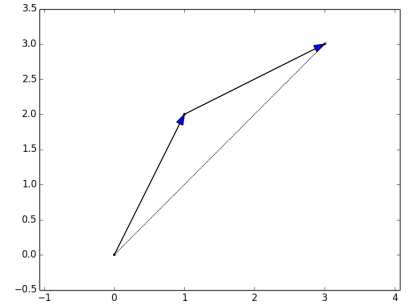
\includegraphics[width=0.5\linewidth]{vecadd}
\end{center}
\end{frame}

%%%%%%%%%%%%%%%%%%%%%%%%%%%%%%%%%%%%%%%%%%%%%%%%%%%%%%%%%%%%%%%%%%%%%%%%
\begin{frame}[fragile]\frametitle{Vector Addition}
\begin{itemize}
\item Implement vector addition
\item Hint: `zip' two vectors and use List Comprehension
\end{itemize}
\begin{lstlisting}
def vector_add(v, w):
	:
	return [...]
vv = [ 1, 2,3]
ww = [3,2,1]
result = vector_add(vv,ww)
print("Vector Addition {}".format(result))
\end{lstlisting}
\end{frame}


%%%%%%%%%%%%%%%%%%%%%%%%%%%%%%%%%%%%%%%%%%%%%%%%%%%%%%%%%%%%%%%%%%%%%%%%
\begin{frame}[fragile]\frametitle{Vector Addition}
Solution:
\begin{lstlisting}
def vector_add(v, w):
    """adds corresponding elements"""
    return [v_i + w_i
            for v_i, w_i in zip(v, w)]
\end{lstlisting}
Vector Addition [4, 4, 4]
\end{frame}

%%%%%%%%%%%%%%%%%%%%%%%%%%%%%%%%%%%%%%%%%%%%%%%%%%%%%%%%%%%%%%%%%%%%%%%%
\begin{frame}[fragile]\frametitle{Vector Subtraction}
\begin{itemize}
\item Implement vector subtraction
\item Hint: its an addition with second vector negated
\end{itemize}
\begin{lstlisting}
def vector_subtract(v, w):
	:
	return [...]
vv = [ 1, 2,3]
ww = [3,2,1]
result = vector_subtract(vv,ww)
print("Vector Subtraction {}".format(result))
\end{lstlisting}
\end{frame}

%%%%%%%%%%%%%%%%%%%%%%%%%%%%%%%%%%%%%%%%%%%%%%%%%%%%%%%%%%%%%%%%%%%%%%%%
\begin{frame}[fragile]\frametitle{Vector Subtraction}
Solution:
\begin{lstlisting}
def vector_subtract(v, w):
    """subtracts corresponding elements"""
    return [v_i - w_i
            for v_i, w_i in zip(v, w)]
\end{lstlisting}
Vector Subtraction [-2, 0, 2]
\end{frame}

%%%%%%%%%%%%%%%%%%%%%%%%%%%%%%%%%%%%%%%%%%%%%%%%%%%%%%%%%%%%%%%%%%%%%%%%
\begin{frame}[fragile]\frametitle{Vectors Summation}
\begin{itemize}
\item Implement vector summation
\item Component-wise sum a list of vectors
\item Result is a new vector whose first element is the sum of all the first elements, and so on
\end{itemize}
\begin{lstlisting}
def vector_sum(vectors):
	:
	return [...]
vecs = [[ 1, 2,3],[3,2,1],[3,2,-1]]
result = vector_sum(vecs)
print("Vectors Sum {}".format(result))
\end{lstlisting}
\end{frame}

%%%%%%%%%%%%%%%%%%%%%%%%%%%%%%%%%%%%%%%%%%%%%%%%%%%%%%%%%%%%%%%%%%%%%%%%
\begin{frame}[fragile]\frametitle{Vectors Summation}
Solution:
\begin{lstlisting}
def vector_sum(vectors):
    """sums all corresponding elements"""
    result = vectors[0]
    for vector in vectors[1:]:     
        result = vector_add(result, vector)    
    return result
\end{lstlisting}
Vectors Sum [7, 6, 3]
\end{frame}

%%%%%%%%%%%%%%%%%%%%%%%%%%%%%%%%%%%%%%%%%%%%%%%%%%%%%%%%%%%%%%%%%%%%%%%%
\begin{frame}[fragile]\frametitle{Scalar Multiplication}
\begin{itemize}
\item Implement scalar multiplication of a vector
\item Component-wise multiplication
\end{itemize}
\begin{lstlisting}
def scalar_multiply(c, v):
	:
	return [...]
vv = [ 1, 2,3]
cc = 4
result =  scalar_multiply(cc,vv)
print("Scalar Multiply {}".format(result))
\end{lstlisting}
\end{frame}

%%%%%%%%%%%%%%%%%%%%%%%%%%%%%%%%%%%%%%%%%%%%%%%%%%%%%%%%%%%%%%%%%%%%%%%%
\begin{frame}[fragile]\frametitle{Scalar Multiplication}
Solution:
\begin{lstlisting}
def scalar_multiply(c, v):
    """c is a number, v is a vector"""
    return [c * v_i for v_i in v]
\end{lstlisting}
Scalar Multiply [4, 8, 12]
\end{frame}

%%%%%%%%%%%%%%%%%%%%%%%%%%%%%%%%%%%%%%%%%%%%%%%%%%%%%%%%%%%%%%%%%%%%%%%%
\begin{frame}[fragile]\frametitle{Vectors Mean}
\begin{itemize}
\item Component-wise means of a list of (same-sized) vectors:
\item Hint: use \lstinline|vector_sum| to add all up, then use \lstinline|scalar_multiply| to compute mean
\end{itemize}
\begin{lstlisting}
def vector_mean(vectors):
	:
	return [...]
vecs = [[ 1, 2,3],[3,2,1],[3,2,-1]]
result = vector_mean(vecs)
print("Vectors Mean {}".format(result))
\end{lstlisting}
\end{frame}

%%%%%%%%%%%%%%%%%%%%%%%%%%%%%%%%%%%%%%%%%%%%%%%%%%%%%%%%%%%%%%%%%%%%%%%%
\begin{frame}[fragile]\frametitle{Vectors Mean}
Solution:
\begin{lstlisting}
def vector_mean(vectors):
    """compute the vector whose ith element is the mean of the ith elements of the input vectors"""
    n = len(vectors)
    return scalar_multiply(1/n, vector_sum(vectors))
\end{lstlisting}
Vectors Mean [2.333333333333333, 2.0, 1.0]
\end{frame}

%%%%%%%%%%%%%%%%%%%%%%%%%%%%%%%%%%%%%%%%%%%%%%%%%%%%%%%%%%%%%%%%%%%%%%%%
\begin{frame}[fragile]\frametitle{Vector Multiplication}
\begin{itemize}
\item  Dot Product : Output? Meaning?
\item  Cross Product : Output? Meaning?
\end{itemize}
$$a.b = |a| \times |b| \times cos(\theta)$$
$$a \times b = |a| \times |b| \times sin(\theta)\hat{n}$$
\end{frame}


%%%%%%%%%%%%%%%%%%%%%%%%%%%%%%%%%%%%%%%%%%%%%%%%%%%%%%%%%%%%%%%%%%%%%%%%
\begin{frame}[fragile]\frametitle{Dot Product}
\begin{itemize}
\item The Dot Product gives a number as an answer (a ``scalar'', not a vector). 
\item $a.b = a_x \times b_x + a_y \times b_y$
\item So we multiply the x's, multiply the y's, then add.
\item Cant multiply unless they are in same direction.
\item So, one of them is projected over another using $cos(\theta)$
\end{itemize}
\begin{center}
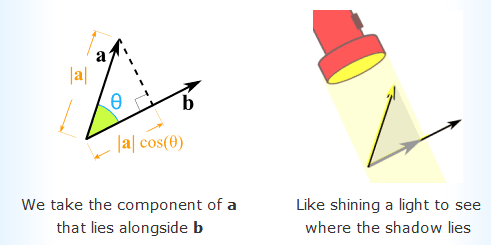
\includegraphics[width=0.5\linewidth]{vecproj}
\end{center}
If vectors are at right angles?
\tiny{(Reference: https://www.mathsisfun.com/algebra/vectors-dot-product.html)}
\end{frame}


%%%%%%%%%%%%%%%%%%%%%%%%%%%%%%%%%%%%%%%%%%%%%%%%%%%%%%%%%%%%%%%%%%%%%%%%
\begin{frame}[fragile]\frametitle{Dot Product}
\begin{itemize}
\item  The dot product of two vectors is the sum of their component-wise products. 
\item Hint: Similar to \lstinline|vector_add| but with a difference in return type
\end{itemize}
\begin{lstlisting}
def dot(v, w):
	:
	return ...
vv = [ 1, 2,3]
ww = [3,2,1]
result = dot(vv,ww)
print("Dot Product {}".format(result))
\end{lstlisting}
\end{frame}

%%%%%%%%%%%%%%%%%%%%%%%%%%%%%%%%%%%%%%%%%%%%%%%%%%%%%%%%%%%%%%%%%%%%%%%%
\begin{frame}[fragile]\frametitle{Dot Product}
Solution:
\begin{lstlisting}
def dot(v, w):
    """v_1 * w_1 + ... + v_n * w_n"""
    return sum(v_i * w_i
               for v_i, w_i in zip(v, w))
\end{lstlisting}
Dot Product 10.
%%\end{frame}
%%
%%%%%%%%%%%%%%%%%%%%%%%%%%%%%%%%%%%%%%%%%%%%%%%%%%%%%%%%%%%%%%%%%%%%%%%%%%
%%\begin{frame}[fragile]\frametitle{Dot Product}
%%Its a projection
%%\begin{center}
%%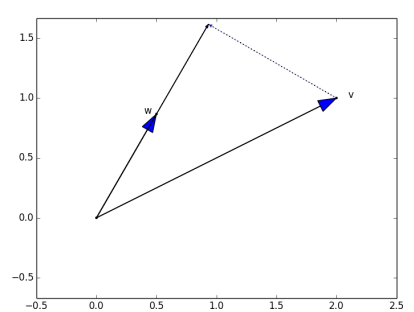
\includegraphics[width=0.5\linewidth]{vecdot}
%%\end{center}

Easy to compute a vector's sum of squares:
\begin{lstlisting}
def sum_of_squares(v):
    """v_1 * v_1 + ... + v_n * v_n"""
    return dot(v, v)
\end{lstlisting}
\end{frame}

%%%%%%%%%%%%%%%%%%%%%%%%%%%%%%%%%%%%%%%%%%%%%%%%%%%%%%%%%%%%%%%%%%%%%%%%%%
%%\begin{frame}[fragile]\frametitle{Dot Product}
%%Easy to compute a vector's sum of squares:
%%\begin{lstlisting}
%%def sum_of_squares(v):
%%    """v_1 * v_1 + ... + v_n * v_n"""
%%    return dot(v, v)
%%\end{lstlisting}
%%\end{frame}

%%%%%%%%%%%%%%%%%%%%%%%%%%%%%%%%%%%%%%%%%%%%%%%%%%%%%%%%%%%%%%%%%%%%%%%%
\begin{frame}[fragile]\frametitle{Magnitude of a Vector}
\begin{lstlisting}
import math
def magnitude(v):
    return math.sqrt(sum_of_squares(v)) 
\end{lstlisting}
\end{frame}

%%%%%%%%%%%%%%%%%%%%%%%%%%%%%%%%%%%%%%%%%%%%%%%%%%%%%%%%%%%%%%%%%%%%%%%%
\begin{frame}[fragile]\frametitle{Distance Between Vectors}
\begin{itemize}
\item  Formula:
$ \sqrt{(v_1 - w_1)^2 + \ldots (v_n - w_n)^2}$
\item Hint: First use \lstinline|vector_subtract| and then \lstinline|sum_of_squares|
\item For now, do not bother about normalizing it with product of their magnitudes.

\end{itemize}
\begin{lstlisting}
def squared_distance(v, w):
	:
	return ...
vv = [ 1, 2,3]
ww = [3,2,1]
result = squared_distance(vv,ww)
print("Squared Distance {}".format(result))
\end{lstlisting}
\end{frame}

%%%%%%%%%%%%%%%%%%%%%%%%%%%%%%%%%%%%%%%%%%%%%%%%%%%%%%%%%%%%%%%%%%%%%%%%
\begin{frame}[fragile]\frametitle{Distance}

\begin{lstlisting}
def squared_distance(v, w):
    """(v_1 - w_1) ** 2 + ... + (v_n - w_n) ** 2"""
    return sum_of_squares(vector_subtract(v, w))
    
def distance(v, w):
   return math.sqrt(squared_distance(v, w))
\end{lstlisting}
or
\begin{lstlisting}
def distance(v, w):
    return magnitude(vector_subtract(v, w))
\end{lstlisting}
Squared Distance 8
\end{frame}

%%%%%%%%%%%%%%%%%%%%%%%%%%%%%%%%%%%%%%%%%%%%%%%%%%%%%%%%%%%%%%%%%%%%%%%%
\begin{frame}[fragile]\frametitle{Matrices}
\begin{itemize}
\item  A matrix is a two-dimensional collection of numbers. 
\item list of  lists, with each inner list having the same size and representing a row of the
matrix.
\item  If  $A$  is a matrix, then  $A[i][j]$  is the element in the $i$th row and the $j$th column.
\end{itemize}
\begin{lstlisting}
A = [[1, 2, 3],  # A has 2 rows and 3 columns
     [4, 5, 6]]
B = [[1, 2],     # B has 3 rows and 2 columns
     [3, 4],
     [5, 6]]
\end{lstlisting}
\end{frame}

%%%%%%%%%%%%%%%%%%%%%%%%%%%%%%%%%%%%%%%%%%%%%%%%%%%%%%%%%%%%%%%%%%%%%%%%
\begin{frame}[fragile]\frametitle{Matrices}
\begin{itemize}
\item  Python lists, being `0' indexed, first row of a matrix ``row 0'' and the first column ``column 0''.
\item  matrix  $A$  has  $len(A)$  rows and  $len(A[0])$ columns, which we consider its  shape
\end{itemize}
\begin{lstlisting}
def shape(A):
    num_rows = len(A)
    num_cols = len(A[0]) if A else 0 
    return num_rows, num_cols
\end{lstlisting}
Numpy and Pandas Dataframes have in built matrix functionality needed for Data Science
\end{frame}


% \section[Basics]{Basics}
% %%%%%%%%%%%%%%%%%%%%%%%%%%%%%%%%%%%%%%%%%%%%%%%%%%%%%%%%%%%%%%%%%%%%%%%%%%%%%%%%%%
\begin{frame}[fragile]\frametitle{}
\begin{center}
{\Large Land of Mathematics}
\end{center}
\end{frame}

%%%%%%%%%%%%%%%%%%%%%%%%%%%%%%%%%%%%%%%%%%%%%%%%%%%%%%%%%%%
 \begin{frame}[fragile]\frametitle{High School Mathematics}
\begin{itemize}
\item Which Mathematics related words do you remember?
\item Which Mathematics related branches do you know?
\item Mathematics is the Language of Science.
\item It provides grammar, words, structure.
\item Our first encounter: Equations \ldots
\end{itemize}
\end{frame}

% TBD : History of Mathematics, Why Mathematics, etc.
% %%%%%%%%%%%%%%%%%%%%%%%%%%%%%%%%%%%%%%%%%%%%%%%%%%%%%%%%%%%%%%%%%%%%%%%%%%%%%%%%%%
\begin{frame}[fragile]\frametitle{}
\begin{center}
{\Large Numbers}
\end{center}
\end{frame}

%%%%%%%%%%%%%%%%%%%%%%%%%%%%%%%%%%%%%%%%%%%%%%%%%%%%%%%%%%%
 \begin{frame}[fragile]\frametitle{Numbers}
\begin{itemize}
\item $ x = 3 \Rightarrow \mathbb{N}$: Natural numbers: 1,2,3,\ldots
\item $ x + 5 = 3 \Rightarrow \mathbb{Z}$: Integers: -1,0,1,2,3,\ldots
\item $ 2x = 3 \Rightarrow \mathbb{Q}$: Rational numbers, ratios: $\frac{3}{2},\frac{1}{3}$,\ldots
\item $ x^2 = 2 \Rightarrow \mathbb{P}$: Irrational numbers, cannot be expressed as ratios: $\sqrt{2},\sqrt[3]{2}$,\ldots.
\item $\pi, e \Rightarrow \mathbb{R}$: Real numbers, these cannot be represented by polynomials, cannot be roots, etc.
\item $ x^2 +1 = 0 \Rightarrow \mathbb{C}$: Complex numbers: $i,2+3i$,\ldots.All polynomials have roots in $\mathbb{C}$
\end{itemize}

$\mathbb{N} \subseteq \mathbb{Z} \subseteq \mathbb{Q} \subseteq \mathbb{P} \subseteq \mathbb{R} \subseteq \mathbb{C} $

Note: all the coefficients in the equation are $\mathbb{N}$ but the resultant $x$ is of different types.
\end{frame}
% %%%%%%%%%%%%%%%%%%%%%%%%%%%%%%%%%%%%%%%%%%%%%%%%%%%%%%%%%%%%%%%%%%%%%%%%%%%%%%%%%%
\begin{frame}[fragile]\frametitle{}
\begin{center}
{\Large Equations}
\end{center}
\end{frame}

%%%%%%%%%%%%%%%%%%%%%%%%%%%%%%%%%%%%%%%%%%%%%%%%%%%%%%%%%%%
 \begin{frame}[fragile]\frametitle{Algebra}
\begin{itemize}
\item Equation 'equates' two expressions. E.g. $3x+4=10$
\item We solve equations for unknowns such as $x$
\item $x$ in the equation above have coefficient $3$.
\item Others like $4$ and $10$ are constants.
\end{itemize}
\end{frame}

%%%%%%%%%%%%%%%%%%%%%%%%%%%%%%%%%%%%%%%%%%%%%%%%%%%%%%%%%%%
 \begin{frame}[fragile]\frametitle{Equations}
 $3x+4=10$
\begin{itemize}
\item To Solve, we isolate $x$ on one side by operations.
\item $3x + 4 - 4 = 10 - 4$
\item Although a short hand way is just to transfer $4$ from one side to other and changing the sign.
\item $3x = 6$
\item In case of coefficients, you divide after crossing the $=$
\item $3x/3 = 6/3$
\item $x = 2$
\item To test, plug $x=2$, back in the original equation and see if both sides 'equate'.
\end{itemize}
\end{frame}

%%%%%%%%%%%%%%%%%%%%%%%%%%%%%%%%%%%%%%%%%%%%%%%%%%%%%%%%%%%
 \begin{frame}[fragile]\frametitle{The Distributive Property}
 
\begin{itemize}
\item $3(x+2)=18$ is same as $3x + 6 = 18$
\item Intuitively we multiply everything from outside, as if its a coefficient.
\item Now instead of just 3 I have another expression to multiply $(3x + 3)(x+2) = 18$
\item Same distributive property works?
\end{itemize}
\end{frame}

%%%%%%%%%%%%%%%%%%%%%%%%%%%%%%%%%%%%%%%%%%%%%%%%%%%%%%%%%%%
 \begin{frame}[fragile]\frametitle{Two Variables}
 
\begin{itemize}
\item $2y - 4x = 2$
\item How to solve?
\item Can we solve?
\end{itemize}
\end{frame}

%%%%%%%%%%%%%%%%%%%%%%%%%%%%%%%%%%%%%%%%%%%%%%%%%%%%%%%%%%%
 \begin{frame}[fragile]\frametitle{Two Variables}
 
\begin{itemize}
\item $2y - 4x = 2$
\item Isolate $y$ first 
\item $2y = 2 + 4x$
\item $y = 1 + 2x$
\item Thats y's definition in terms of x.
\item For any x, y can be calculated.
\item x, y if plotted form a line, thus the original equation is called as Linear Equation.
\end{itemize}
\end{frame}

%%%%%%%%%%%%%%%%%%%%%%%%%%%%%%%%%%%%%%%%%%%%%%%%%%%%%%%%%%%
 \begin{frame}[fragile]\frametitle{Line Plot}
 
\begin{itemize}
\item X intercept is where line crosses x axis, where y is 0 (put in the eqn)
\item Y intercept is where line crosses y axis, where x is 0 (put in the eqn)
\end{itemize}
\begin{center}
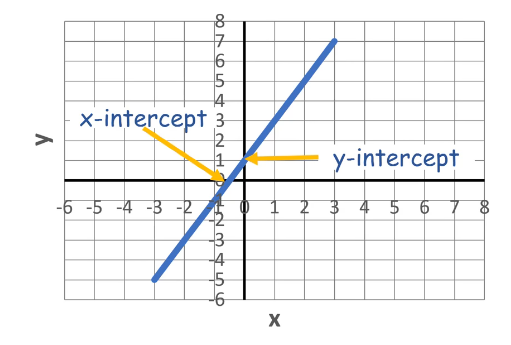
\includegraphics[width=0.5\linewidth,keepaspectratio]{lineqn}
\end{center}
\end{frame}


%%%%%%%%%%%%%%%%%%%%%%%%%%%%%%%%%%%%%%%%%%%%%%%%%%%%%%%%%%%
 \begin{frame}[fragile]\frametitle{Line Plot}
 
\begin{itemize}
\item Slope is change in y per change in x
\item Calculated using any two points.
\item Slope-Intercept form is $y = mx + b$
\end{itemize}
\begin{center}
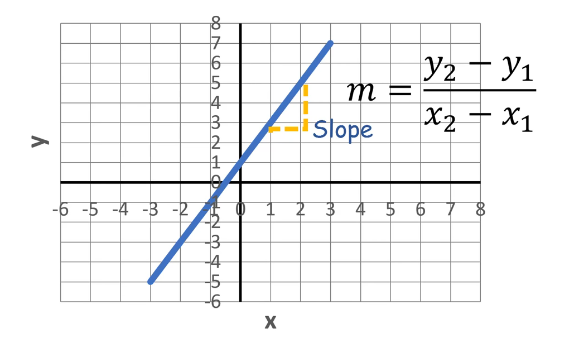
\includegraphics[width=0.5\linewidth,keepaspectratio]{lineqn1}
\end{center}
\end{frame}

%%%%%%%%%%%%%%%%%%%%%%%%%%%%%%%%%%%%%%%%%%%%%%%%%%%%%%%%%%%
 \begin{frame}[fragile]\frametitle{Exercise}
Find slope and both intercepts of $2y + 3 = 3x -1 $
\end{frame}

%%%%%%%%%%%%%%%%%%%%%%%%%%%%%%%%%%%%%%%%%%%%%%%%%%%%%%%%%%%
 \begin{frame}[fragile]\frametitle{Exercise}
\begin{lstlisting}
import pandas as pd

# Create a dataframe with an x column containing values from -10 to 10
df = pd.DataFrame ({'x': range(-10, 11)})

# Add a y column by applying the solved equation to x
df['y'] = (3*df['x'] - 4) / 2

print(df)
\end{lstlisting}
\end{frame}

%%%%%%%%%%%%%%%%%%%%%%%%%%%%%%%%%%%%%%%%%%%%%%%%%%%%%%%%%%%
 \begin{frame}[fragile]\frametitle{Exercise}
\begin{lstlisting}
from matplotlib import pyplot as plt

plt.plot(df.x, df.y, color="grey", marker = "o")
plt.xlabel('x')
plt.ylabel('y')
plt.grid()
plt.show()
\end{lstlisting}
\begin{center}
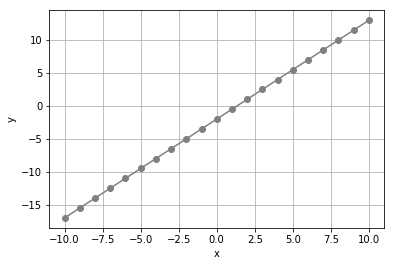
\includegraphics[width=0.5\linewidth,keepaspectratio]{lineqn2}
\end{center}
\end{frame}


%%%%%%%%%%%%%%%%%%%%%%%%%%%%%%%%%%%%%%%%%%%%%%%%%%%%%%%%%%%
 \begin{frame}[fragile]\frametitle{System of Equations}
 9 items cost 75c, how many are apples and how many oranges?
\begin{center}
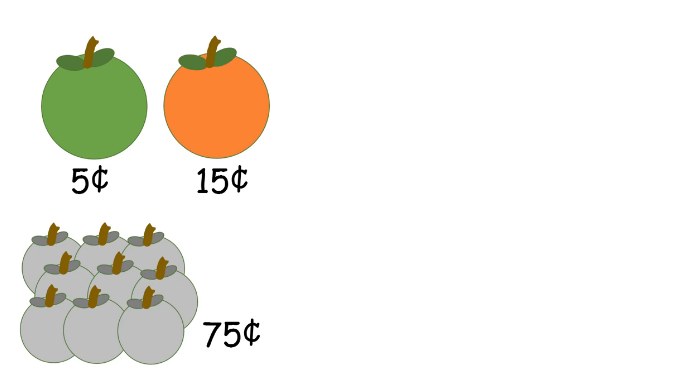
\includegraphics[width=0.5\linewidth,keepaspectratio]{lineqn3}

{\tiny (Ref: Essentials of Mathematics - DAT 256 EdX)}
\end{center}
\end{frame}

%%%%%%%%%%%%%%%%%%%%%%%%%%%%%%%%%%%%%%%%%%%%%%%%%%%%%%%%%%%
 \begin{frame}[fragile]\frametitle{System of Equations}
Let number of apples be x and oranges be y.
\begin{center}
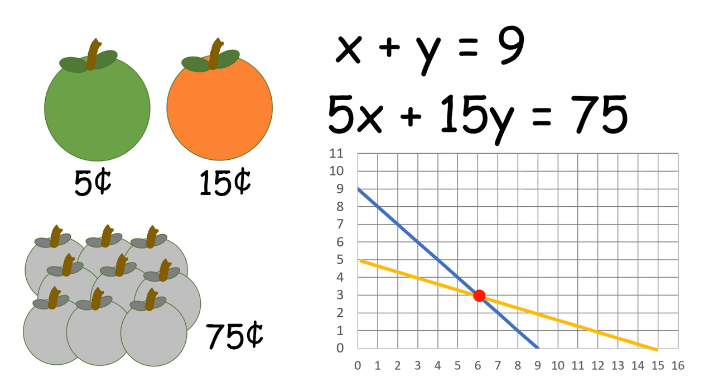
\includegraphics[width=0.5\linewidth,keepaspectratio]{lineqn4}

{\tiny (Ref: Essentials of Mathematics - DAT 256 EdX)}
\end{center}
Blue line represents $x+y=9$ and yellow line $5x+15y=75$. Their intersection, the common point shared by two equations, is the solution.
\end{frame}

%%%%%%%%%%%%%%%%%%%%%%%%%%%%%%%%%%%%%%%%%%%%%%%%%%%%%%%%%%%
 \begin{frame}[fragile]\frametitle{System of Equations}
System of Linear equations can be solved, apart from line intersection method, by elimination method.
\begin{center}
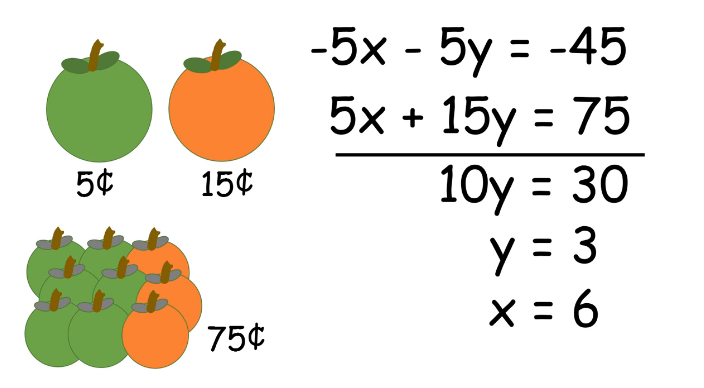
\includegraphics[width=0.5\linewidth,keepaspectratio]{lineqn5}

{\tiny (Ref: Essentials of Mathematics - DAT 256 EdX)}
\end{center}
Make one of the equations (say, first) as NEGATIVE of the other in one variable, so that their addition cancels it out, leaving only one variable. Easy to find solution. Put that value back in the original equation, to get the other variable value.
\end{frame}

%%%%%%%%%%%%%%%%%%%%%%%%%%%%%%%%%%%%%%%%%%%%%%%%%%%%%%%%%%%
 \begin{frame}[fragile]\frametitle{Exercise}
Solve $x + y = 16$ and $10x + 25y = 250$
\end{frame}





%%%%%%%%%%%%%%%%%%%%%%%%%%%%%%%%%%%%%%%%%%%%%%%%%%%%%%%%%%%%%%%%%%%%%%%%%%%%%%%%%%
\begin{frame}[fragile]\frametitle{}
\begin{center}
{\Large Polynomials}
\end{center}
\end{frame}



%%%%%%%%%%%%%%%%%%%%%%%%%%%%%%%%%%%%%%%%%%%%%%%%%%%%%%%%%%%
 \begin{frame}[fragile]\frametitle{Polynomials}
\begin{itemize}
\item Polynomials = Many (Poly) terms
\item Terms can be constants, coefficients with variables, some with exponentials
\item $6 + 4x - 3 x^2$
\item Any arithmetic operators can be used
\item Standard form is in decreasing powers $-3x^2 + 4x + 6$
\end{itemize}
\end{frame}

%%%%%%%%%%%%%%%%%%%%%%%%%%%%%%%%%%%%%%%%%%%%%%%%%%%%%%%%%%%
 \begin{frame}[fragile]\frametitle{Polynomial Operations}
Addition or subtraction of polynomials is those operations on similar exponential terms
\begin{center}
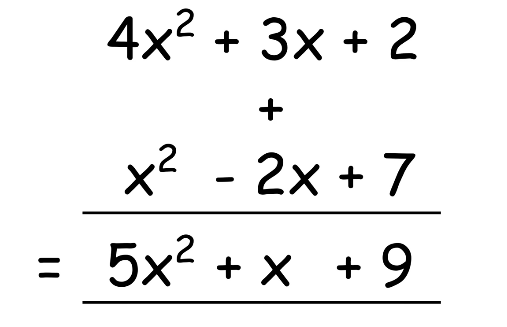
\includegraphics[width=0.6\linewidth,keepaspectratio]{polyadd}
\end{center}
\end{frame}


%%%%%%%%%%%%%%%%%%%%%%%%%%%%%%%%%%%%%%%%%%%%%%%%%%%%%%%%%%%
 \begin{frame}[fragile]\frametitle{Polynomial Operations}
For multiplication, each term in first is multiplied with all in the second, then added.
\begin{center}
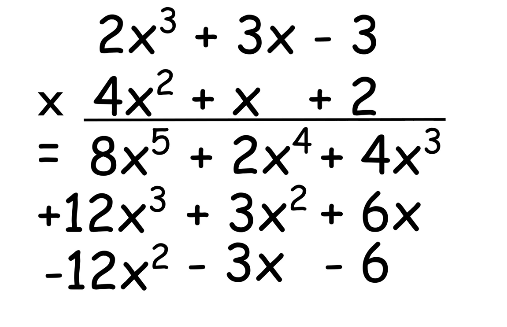
\includegraphics[width=0.6\linewidth,keepaspectratio]{polymul}
\end{center}
$8x^5 + 2x^4 + 16x^3-9x^2+3x-6$
\end{frame}

%%%%%%%%%%%%%%%%%%%%%%%%%%%%%%%%%%%%%%%%%%%%%%%%%%%%%%%%%%%
 \begin{frame}[fragile]\frametitle{Polynomial Operations}
Division by a single term
\begin{center}
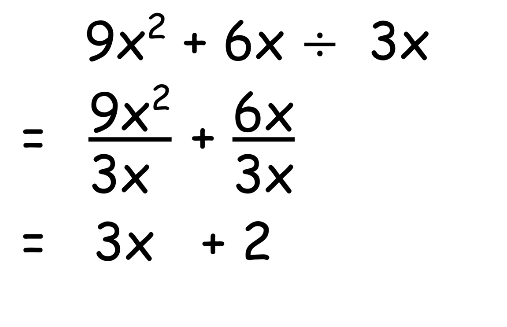
\includegraphics[width=0.6\linewidth,keepaspectratio]{polydiv}
\end{center}
\end{frame}

%%%%%%%%%%%%%%%%%%%%%%%%%%%%%%%%%%%%%%%%%%%%%%%%%%%%%%%%%%%
 \begin{frame}[fragile]\frametitle{Polynomial Operations}
Division by a complex term. Find the factor with highest power term, subtract, repeat on remainder.
\begin{center}
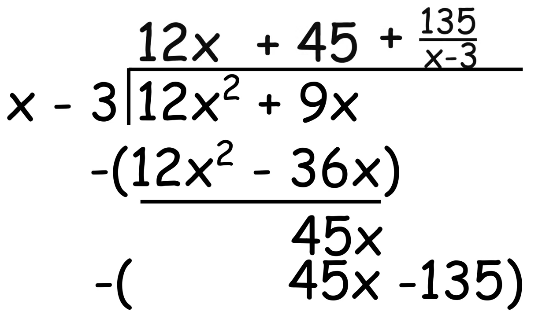
\includegraphics[width=0.6\linewidth,keepaspectratio]{polydiv1}
\end{center}
\end{frame}

%%%%%%%%%%%%%%%%%%%%%%%%%%%%%%%%%%%%%%%%%%%%%%%%%%%%%%%%%%%%%%%%%%%%%%%%%%%%%%%%%%
\begin{frame}[fragile]\frametitle{}
\begin{center}
{\Large Factorization}
\end{center}
\end{frame}



%%%%%%%%%%%%%%%%%%%%%%%%%%%%%%%%%%%%%%%%%%%%%%%%%%%%%%%%%%%
 \begin{frame}[fragile]\frametitle{Factors}
\begin{itemize}
\item Restating expression in terms of multiplication of multiple expressions.
\item Eg $6 = 1 \times 6 = 2 \times 3$
\item 1,2,3,6 are factors of 6
\item Similarly $1x,2x,3x,6x$ are factors of $6x^2$
\item What are common factors of 6 and 15?
\item 1 and 3. 
\item 3 is GCF  (Greatest Common Factor )
\item ma saa vii : mahattam samanya vibhajak
\end{itemize}
\end{frame}

%%%%%%%%%%%%%%%%%%%%%%%%%%%%%%%%%%%%%%%%%%%%%%%%%%%%%%%%%%%
 \begin{frame}[fragile]\frametitle{Simplifying Polynomials}
\begin{itemize}
\item GCF of $12x$ and $20x^2$ ?
\item GCF of coefficients into lowest variable power term ie $4x$
\item Useful in simplifying Polynomials
\item $9x + 12y$
\item GCF is 3
\item $= 3(3x) + 3(4y) = 3(3x+4y)$
\end{itemize}
\end{frame}

%%%%%%%%%%%%%%%%%%%%%%%%%%%%%%%%%%%%%%%%%%%%%%%%%%%%%%%%%%%%%%%%%%%%%%%%%%%%%%%%%%
\begin{frame}[fragile]\frametitle{}
\begin{center}
{\Large Quadratic Equations}
\end{center}
\end{frame}

%%%%%%%%%%%%%%%%%%%%%%%%%%%%%%%%%%%%%%%%%%%%%%%%%%%%%%%%%%%
 \begin{frame}[fragile]\frametitle{Quadratic Equations}
 Highest order term is Square.e.g Parabola is open at top, closed at bottom.
\begin{center}
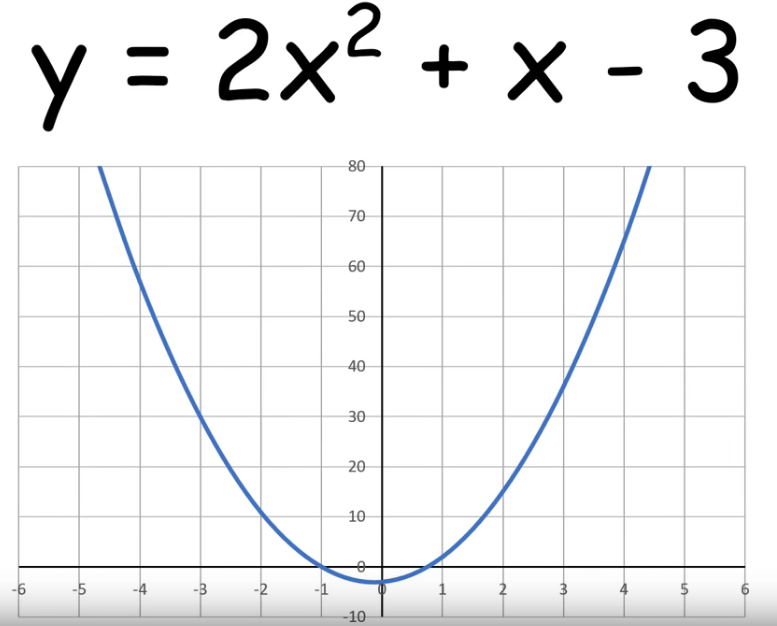
\includegraphics[width=0.6\linewidth,keepaspectratio]{para1}
\end{center}

\end{frame}


%%%%%%%%%%%%%%%%%%%%%%%%%%%%%%%%%%%%%%%%%%%%%%%%%%%%%%%%%%%
 \begin{frame}[fragile]\frametitle{Quadratic Equations}
With negative highest term similar Parabola is open at bottom, closed at top.
\begin{center}
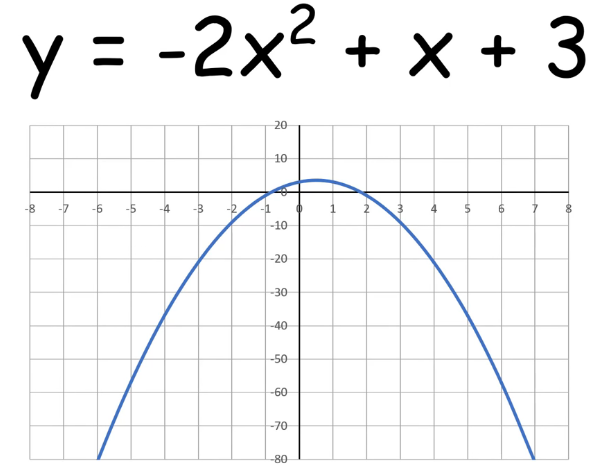
\includegraphics[width=0.6\linewidth,keepaspectratio]{para2}
\end{center}

\end{frame}

%%%%%%%%%%%%%%%%%%%%%%%%%%%%%%%%%%%%%%%%%%%%%%%%%%%%%%%%%%%
 \begin{frame}[fragile]\frametitle{Exercise}
$y = 2x^2 + 2x - 4$

\begin{lstlisting}
import pandas as pd

# Create a dataframe with an x column containing values to plot
df = pd.DataFrame ({'x': range(-9, 9)})

# Add a y column by applying the quadratic equation to x
df['y'] = 2*df['x']**2 + 2 *df['x'] - 4

# Plot the line
%matplotlib inline
from matplotlib import pyplot as plt

plt.plot(df.x, df.y, color="grey")
plt.xlabel('x')
plt.ylabel('y')
plt.grid()
plt.axhline()
plt.axvline()
plt.show()
\end{lstlisting}
\end{frame}

%%%%%%%%%%%%%%%%%%%%%%%%%%%%%%%%%%%%%%%%%%%%%%%%%%%%%%%%%%%
 \begin{frame}[fragile]\frametitle{Quadratic Equations}
\begin{center}
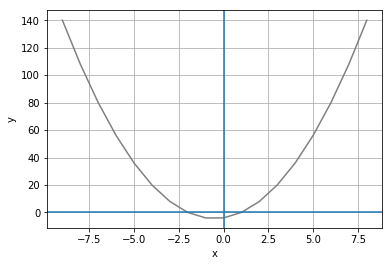
\includegraphics[width=0.6\linewidth,keepaspectratio]{para3}
\end{center}

\end{frame}


% %%%%%%%%%%%%%%%%%%%%%%%%%%%%%%%%%%%%%%%%%%%%%%%%%%%%%%%%%%%%%%%%%%%%%%%%%%%%%%%%%%
\begin{frame}[fragile]\frametitle{}
\begin{center}
{\Large Exponentials}
\end{center}
\end{frame}



%%%%%%%%%%%%%%%%%%%%%%%%%%%%%%%%%%%%%%%%%%%%%%%%%%%%%%%%%%%
 \begin{frame}[fragile]\frametitle{Power}
\begin{itemize}
\item $3 \times 3 = 3^2 = 9$
\item $3 \times 3 \times 3 = 3^3 = 27$
\item $4^7 = 16384$ here,  4 is the base, and 7 is the power or exponent in this expression.
\item The 'raised to' can be seen as whole number.
\item Can it be a fraction?
\item Can it be negative?
\end{itemize}
\end{frame}

%%%%%%%%%%%%%%%%%%%%%%%%%%%%%%%%%%%%%%%%%%%%%%%%%%%%%%%%%%%
 \begin{frame}[fragile]\frametitle{Radicals (Roots)}

\begin{itemize}
\item Sometimes you'll need to calculate one or other of the elements themselves.
\item $?^2 = 9$
\item This expression is asking, given a number (9) and an exponent (2), what's the base? 
\item In other words, which number multiplied by itself results in 9? 
\item This type of operation is referred to as calculating the root, and in this particular case it's the square root $\sqrt 9 = 3$ 
\item $36^{1/2} =?$
\item $81^{1/3} =?$
\end{itemize}
\end{frame}

%%%%%%%%%%%%%%%%%%%%%%%%%%%%%%%%%%%%%%%%%%%%%%%%%%%%%%%%%%%
 \begin{frame}[fragile]\frametitle{Radicals (Roots)}
\begin{lstlisting}
import math

# Calculate square root of 25
x = math.sqrt(25)
print (x)

# Calculate cube root of 64
cr = round(64 ** (1. / 3))
print(cr)
\end{lstlisting}
\end{frame}


%%%%%%%%%%%%%%%%%%%%%%%%%%%%%%%%%%%%%%%%%%%%%%%%%%%%%%%%%%%
 \begin{frame}[fragile]\frametitle{Logarithms}

\begin{itemize}
\item To determine the exponent for a given number and base. 
\item In other words, how many times do I need to multiply a base number by itself to get the given result.
\item $4^x =16$, what is $x$?
\item Such solutions are found by logarithms
\item $x = \log_4 (16) = 2$
\item Log finds the POWER to given base, of a number.
\item Whats Log of 1000 to base 10?
\end{itemize}
\end{frame}

%%%%%%%%%%%%%%%%%%%%%%%%%%%%%%%%%%%%%%%%%%%%%%%%%%%%%%%%%%%
 \begin{frame}[fragile]\frametitle{Logarithms}
\begin{lstlisting}
import math

# Natural log of 29
print (math.log(29))

# Common log of 100
print(math.log10(100))
\end{lstlisting}
\end{frame}


%%%%%%%%%%%%%%%%%%%%%%%%%%%%%%%%%%%%%%%%%%%%%%%%%%%%%%%%%%%
 \begin{frame}[fragile]\frametitle{Logarithms}
\begin{itemize}
\item We know of log to base 10 and those log tables. But is there  a function/formula?
\item What is a log? Is it defined for all real values?
\item $10^{2.3} = 10^{\frac{23}{10}}$ Thats 10th root of $10^{23}$
\item $10^{-0.07} = \frac{1}{10^{0.07}}$
\item $10^{\sqrt{2}} = 10^{(2^{1/2})}$. Need to approximate $\sqrt{2}$ to some decimal places and then evaluate.
\item $10^x= y$ then $\log y = x$
\item $x$ can be any real number and $y$ will be corresponding unique number.
\end{itemize}
\end{frame}


%%%%%%%%%%%%%%%%%%%%%%%%%%%%%%%%%%%%%%%%%%%%%%%%%%%%%%%%%%%
 \begin{frame}[fragile]\frametitle{Logarithm to base $e$}
\begin{itemize}
\item $\log x = \int_1^x \frac{1}{t} dt$
\item Its area under curve from 1 to $x$. At $x=1$ there is no area thus $\log 1 = 0$
\begin{center}
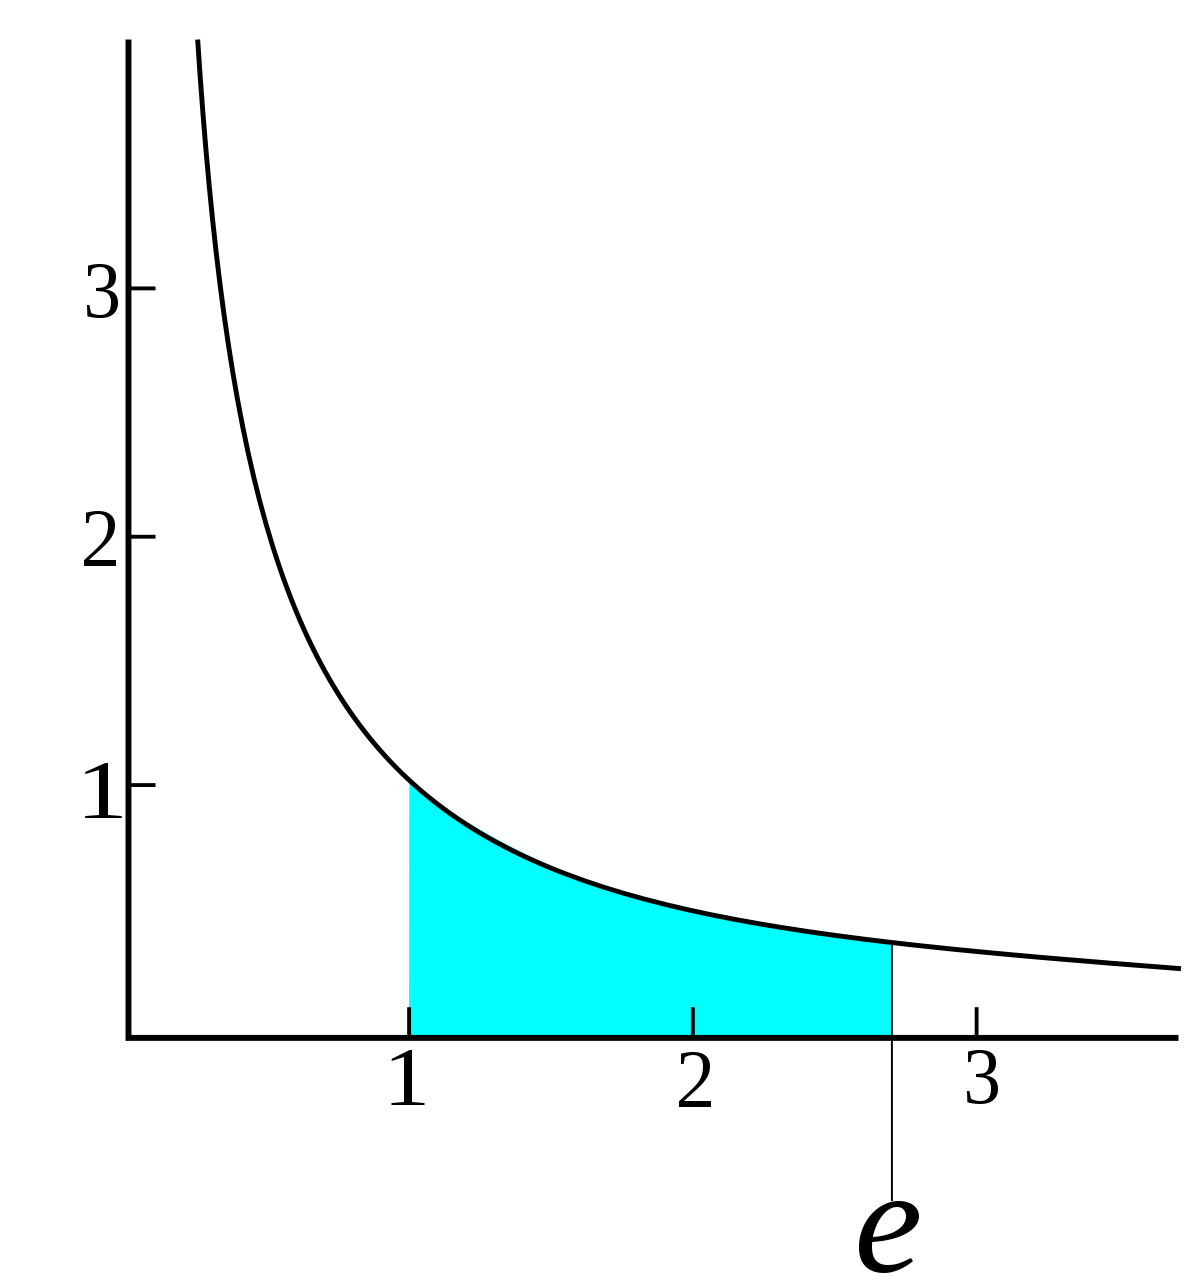
\includegraphics[width=0.4\linewidth,keepaspectratio]{ln}
\end{center}
\item At some $x$ where area is 1, is called as $e$.
\end{itemize}
\end{frame}


%%%%%%%%%%%%%%%%%%%%%%%%%%%%%%%%%%%%%%%%%%%%%%%%%%%%%%%%%%%
 \begin{frame}[fragile]\frametitle{Rules}
Add/Subtract with same power terms
\begin{itemize}
\item We can add coefficients of same power terms
\item $x^2 + 3x^2$ is possible = $4x^2$
\end{itemize}
\end{frame}

%%%%%%%%%%%%%%%%%%%%%%%%%%%%%%%%%%%%%%%%%%%%%%%%%%%%%%%%%%%
 \begin{frame}[fragile]\frametitle{Rules}
Multiply
\begin{itemize}
\item Adds the POWER terms
\item $2x^3 \times 4x^2 = ?$
\item $8x^5$
\item Similarly division is opposite
\item $6x^5 / 3x^2 = 2x^3$
\end{itemize}
\end{frame}

%%%%%%%%%%%%%%%%%%%%%%%%%%%%%%%%%%%%%%%%%%%%%%%%%%%%%%%%%%%
 \begin{frame}[fragile]\frametitle{Exercise}
Reduce $2y = 2x^4 (\frac{x^2 + 2x^2}{x^3})$
\end{frame}
%%%%%%%%%%%%%%%%%%%%%%%%%%%%%%%%%%%%%%%%%%%%%%%%%%%%%%%%%%%
 \begin{frame}[fragile]\frametitle{Solution}
$y = 3x^3$

\begin{lstlisting}
import pandas as pd

df = pd.DataFrame ({'x': range(-10, 11)})

df['y'] = 3*df['x']**3

from matplotlib import pyplot as plt

plt.plot(df.x, df.y, color="magenta")
plt.xlabel('x')
plt.ylabel('y')
plt.grid()
plt.axhline()
plt.axvline()
plt.show()
\end{lstlisting}
\end{frame}

%%%%%%%%%%%%%%%%%%%%%%%%%%%%%%%%%%%%%%%%%%%%%%%%%%%%%%%%%%%
 \begin{frame}[fragile]\frametitle{Plot}
 \begin{lstlisting}
     x     y
0  -10 -3000
1   -9 -2187
2   -8 -1536
3   -7 -1029
4   -6  -648
5   -5  -375
6   -4  -192
7   -3   -81
8   -2   -24
9   -1    -3
10   0     0
11   1     3
12   2    24
13   3    81
14   4   192
15   5   375
16   6   648
17   7  1029
18   8  1536
19   9  2187
20  10  3000
\end{lstlisting}

\end{frame}

%%%%%%%%%%%%%%%%%%%%%%%%%%%%%%%%%%%%%%%%%%%%%%%%%%%%%%%%%%%
 \begin{frame}[fragile]\frametitle{Plot}
\begin{center}
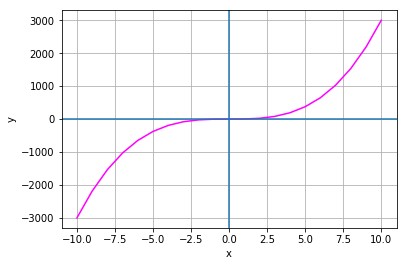
\includegraphics[width=0.8\linewidth,keepaspectratio]{log1}
\end{center}
\end{frame}


%%%%%%%%%%%%%%%%%%%%%%%%%%%%%%%%%%%%%%%%%%%%%%%%%%%%%%%%%%%
 \begin{frame}[fragile]\frametitle{Exercise}
$y = 2^x$

\begin{lstlisting}
import pandas as pd

df = pd.DataFrame ({'x': range(-10, 11)})

df['y'] = 2.0**df['x']

from matplotlib import pyplot as plt

plt.plot(df.x, df.y, color="magenta")
plt.xlabel('x')
plt.ylabel('y')
plt.grid()
plt.axhline()
plt.axvline()
plt.show()
\end{lstlisting}
\end{frame}

%%%%%%%%%%%%%%%%%%%%%%%%%%%%%%%%%%%%%%%%%%%%%%%%%%%%%%%%%%%
 \begin{frame}[fragile]\frametitle{Plot}
 \begin{lstlisting}
     x            y
0  -10     0.000977
1   -9     0.001953
2   -8     0.003906
3   -7     0.007812
4   -6     0.015625
5   -5     0.031250
6   -4     0.062500
7   -3     0.125000
8   -2     0.250000
9   -1     0.500000
10   0     1.000000
11   1     2.000000
12   2     4.000000
13   3     8.000000
14   4    16.000000
15   5    32.000000
16   6    64.000000
17   7   128.000000
18   8   256.000000
19   9   512.000000
20  10  1024.000000
\end{lstlisting}

\end{frame}

%%%%%%%%%%%%%%%%%%%%%%%%%%%%%%%%%%%%%%%%%%%%%%%%%%%%%%%%%%%
 \begin{frame}[fragile]\frametitle{Plot}
\begin{center}
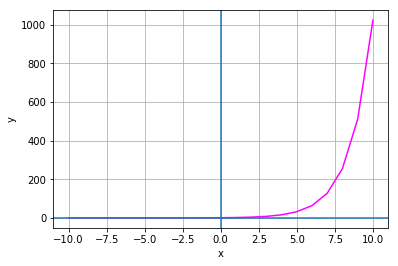
\includegraphics[width=0.8\linewidth,keepaspectratio]{log2}
\end{center}
\end{frame}


%%%%%%%%%%%%%%%%%%%%%%%%%%%%%%%%%%%%%%%%%%%%%%%%%%%%%%%%%%%
 \begin{frame}[fragile]\frametitle{Exercise}
Suppose you deposit Rs 100 in a bank account that earns 5\% interest per year. What would the balance of the account be in twenty years, assuming you don't deposit or withdraw any additional funds?

\begin{lstlisting}
import pandas as pd

# Create a dataframe with 20 years
df = pd.DataFrame ({'Year': range(1, 21)})

# Calculate the balance for each year based on the exponential growth from interest
df['Balance'] = 100 * (1.05**df['Year'])

#Display the dataframe
print(df)

# Plot the line
%matplotlib inline
from matplotlib import pyplot as plt

plt.plot(df.Year, df.Balance, color="green")
plt.xlabel('Year')
plt.ylabel('Balance')
plt.show()
\end{lstlisting}
\end{frame}

%%%%%%%%%%%%%%%%%%%%%%%%%%%%%%%%%%%%%%%%%%%%%%%%%%%%%%%%%%%
 \begin{frame}[fragile]\frametitle{Solution}
\begin{lstlisting}
    Year     Balance
0      1  105.000000
1      2  110.250000
2      3  115.762500
3      4  121.550625
4      5  127.628156
5      6  134.009564
6      7  140.710042
7      8  147.745544
8      9  155.132822
9     10  162.889463
10    11  171.033936
11    12  179.585633
12    13  188.564914
13    14  197.993160
14    15  207.892818
15    16  218.287459
16    17  229.201832
17    18  240.661923
18    19  252.695020
19    20  265.32977
\end{lstlisting}
\end{frame}

%%%%%%%%%%%%%%%%%%%%%%%%%%%%%%%%%%%%%%%%%%%%%%%%%%%%%%%%%%%
 \begin{frame}[fragile]\frametitle{Plot}
\begin{center}
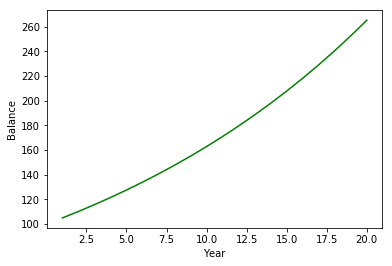
\includegraphics[width=0.8\linewidth,keepaspectratio]{log3}
\end{center}
\end{frame}

% %%%%%%%%%%%%%%%%%%%%%%%%%%%%%%%%%%%%%%%%%%%%%%%%%%%%%%%%%%%%%%%%%%%%%%%%%%%%%%%%%%
\begin{frame}[fragile]\frametitle{}
\begin{center}
{\Large Sets}
\end{center}
\end{frame}

%%%%%%%%%%%%%%%%%%%%%%%%%%%%%%%%%%%%%%%%%%%%%%%%%%%%%%%%%%
\begin{frame}{Sets}
\begin{example}
The set consisting of all positive integers less than $10$ can be denoted by $\{1,2,3,4,5,6,7,8,9\}$.  $\{1,2,3,\ldots,9\}$ is also used since the general pattern is obvious.
\end{example}
\end{frame}


%%%%%%%%%%%%%%%%%%%%%%%%%%%%%%%%%%%%%%%%%%%%%%%%%%%%%%%%%%
\begin{frame}{Sets}
\begin{example}
Members of a set need not be numeric.  The set of all possible outcomes when tossing a coin is  $\{H,T\}$.
\end{example}
\end{frame}

%%%%%%%%%%%%%%%%%%%%%%%%%%%%%%%%%%%%%%%%%%%%%%%%%%%%%%%%%%
\begin{frame}{Set Builder Notation}
For example, $O=\{1,3,5,7,9\}$ can also be written as $$O=\{x: x \text{ is a positive odd integer less than } 10\}.$$

\begin{example} 
\begin{itemize}
\item $A=\{x: x \text{ is a positive even number less than }15\}=\{2,4,6,8,10,12,14\}$.
\item $B=\{n: n \text{ is a positive integer}\}=\{1,2,3,4,5,\ldots\}$.
\item $C=\{2n: n \text{ is a whole number and }1\leq n\leq 4\}=\{2,4,6,8\}$.
\end{itemize}
\end{example}
\end{frame}

%%%%%%%%%%%%%%%%%%%%%%%%%%%%%%%%%%%%%%%%%%%%%%%%%%%%%%%%%%
\begin{frame}{Some Basic Notations}

\begin{itemize}
\item $\emptyset$, The \underline{empty set}\index{empty set} (a set with \textit{no} elements). $\{\quad\}$ is also used. 
\item $\mathbb{N}=\{1,2,3,\ldots\}$, the set of natural numbers.\index{natural number}\index{$\mathbb{N}$}
\item $\mathbb{Z}=\{\ldots,-2,-1,0,1,2,\ldots\}$, the set of integers. \index{integer}\index{$\mathbb{Z}$}
\item $\mathbb{R}$ or $(-\infty,\infty)$, the set of real numbers. \index{real number}\index{$\mathbb{R}$}
\item $[a,b]$, the set of all real numbers $x$ such that $a\leq x \leq b$.
\item $(a,b)$, the set of all real numbers $x$ such that $a< x < b$. 
\item $(a,b]$, the set of all real numbers $x$ such that $a< x \leq  b$. 
\item $[a,b)$, the set of all real numbers $x$ such that $a\leq x< b$. 
\end{itemize}

\end{frame}

%%%%%%%%%%%%%%%%%%%%%%%%%%%%%%%%%%%%%%%%%%%%%%%%%%%%%%%%%%
\begin{frame}{Subsets and Equality}
\begin{definition} A set $A$ is said to be a \underline{subset} of another set $B$  if every element of $A$ is also an element of $B$.  We use the notation $A\subseteq B$.  Two sets $A$ and $B$ are said to be \underline{equal} (notation $A=B$)  if they have the same elements.  In other words, $A$ and $B$ are equal if $A\subseteq B$ and $B\subseteq A$.
\end{definition}
\end{frame}

%%%%%%%%%%%%%%%%%%%%%%%%%%%%%%%%%%%%%%%%%%%%%%%%%%%%%%%%%%
\begin{frame}{Subsets and Equality}
\begin{example} $\{2,3,5\}\subseteq \{-1,2,3,5,7\}$.  However, $\{1,2,3,4\} \nsubseteq \{1,3,4,5,6,7\}$,  because $2\notin \{1,3,4,5,6,7\}$.
\end{example}

\begin{example} By definition, $\mathbb{N}\subseteq \mathbb{Z}\subseteq \mathbb{R}$.
\end{example}
\end{frame}

%%%%%%%%%%%%%%%%%%%%%%%%%%%%%%%%%%%%%%%%%%%%%%%%%%%%%%%%%%
\begin{frame}{Set Operations}
 Let $A$ and $B$ be sets. 
\begin{itemize}
\item The \underline{union} of $A$ and $B$, denoted by $A\cup B$, is the set that contains those elements that are either in $A$ or $B$, or in both.  In other words, $A\cup B=\{x: x\in A \text{ or } x\in B\}$. 
\item The \underline{intersection} of $A$ and $B$, denoted by $A\cap B$, is the set that contains those elements in both $A$ and $B$.  In other words, $A\cap B=\{x: x\in A \text{ and } x\in B\}$. 
\item Two sets are said to be \underline{disjoint} if their intersection is the empty set. 
\item Let $S$ be the universal set (the set of all elements under consideration. It depends on the context).  Then the \underline{complement} $A^c$ of $A$ is defined to be the set of all elements in $S$ that are not in $A$.
\end{itemize}

\end{frame}

%%%%%%%%%%%%%%%%%%%%%%%%%%%%%%%%%%%%%%%%%%%%%%%%%%%%%%%%%%
\begin{frame}{Set Operations, continued}
\begin{example} Let $A=\{1,3,4,5\}$ and $B=\{1,2,3\}$, then $A\cup B=\{1,2,3,4,5\}$ and $A\cap B=\{1,3\}$.
\end{example}

\begin{center}
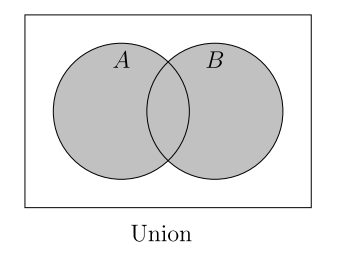
\includegraphics[width=0.4\linewidth,keepaspectratio]{setun}
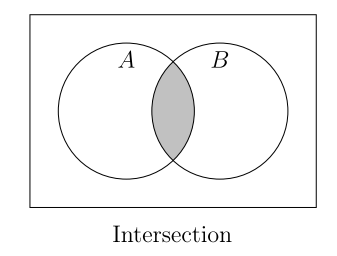
\includegraphics[width=0.4\linewidth,keepaspectratio]{setint}
\end{center}
\end{frame}

%%%%%%%%%%%%%%%%%%%%%%%%%%%%%%%%%%%%%%%%%%%%%%%%%%%%%%%%%%
\begin{frame}{Set Operations, continued}
\begin{example}
If $P=(-\infty, 2)$ and $Q=[-1,\infty)$, then $P\cap Q=[-1,2)$ and $P\cup Q=(-\infty,\infty)=\mathbb{R}$.
\end{example}
\end{frame}

%%%%%%%%%%%%%%%%%%%%%%%%%%%%%%%%%%%%%%%%%%%%%%%%%%%%%%%%%%
\begin{frame}{Set Operations, continued}
\begin{example} Let $O=\{2k+1: k\in \mathbb{Z}\}$ and $E=\{2k: k\in \mathbb{Z}\}$, then $O$ and $E$ are disjoint.  If one takes $\mathbb{Z}$ as the universal set, then $O^c=E$ and $E^c=O$.
\end{example}

\end{frame}


%%%%%%%%%%%%%%%%%%%%%%%%%%%%%%%%%%%%%%%%%%%%%%%%%%%%%%%%%%
\begin{frame}{Cardinality of the Union of Sets}
Let $|S|$ denote the number of elements of a set $S$.  Obviously, $A\cup B$ contains both $A$ and $B$, so $|A\cup B|\geq |A|$ and $|A\cup B|\geq |B|$.  But exactly how many elements are there in $A\cup B$?

\begin{theorem} Let $A,B$ be sets with finitely many elements, then
$$|A\cup B|=|A|+|B|-|A\cap B|.$$  In particular, if $A$ and $B$ are disjoint, then $|A\cup B|=|A|+|B|$.
\end{theorem}

\end{frame}


%%%%%%%%%%%%%%%%%%%%%%%%%%%%%%%%%%%%%%%%%%%%%%%%%%%%%%%%%%
\begin{frame}{Cardinality of the Union of Sets}

\begin{theorem} Let $A,B,C$ be sets with finitely many elements, then
$$|A\cup B \cup C|=|A|+|B|+|C|-|A\cap B|-|B\cap C|-|A\cap C|+|A\cap B \cap C|.$$ 
\end{theorem}
\end{frame}


%%%%%%%%%%%%%%%%%%%%%%%%%%%%%%%%%%%%%%%%%%%%%%%%%%%%%%%%%%%%%%%%%%%%%%%%%%%%%%%%%%
\begin{frame}[fragile]\frametitle{}
\begin{center}
{\Large Probability}
\end{center}
\end{frame}

%%%%%%%%%%%%%%%%%%%%%%%%%%%%%%%%%%%%%%%%%%%%%%%%%%%%%%%%%%
\begin{frame}{Why Probability?}
\begin{itemize}
\item Real life scenarios are inherently random or too complex to be completely known. 
\item If you knew every ``Physics'' aspect of motion of a dice, you could predict the outcome, deterministically.
\item However this can never be done in practice, so there is a CHANCE of something happening.
\end{itemize}
\end{frame}

%%%%%%%%%%%%%%%%%%%%%%%%%%%%%%%%%%%%%%%%%%%%%%%%%%%%%%%%%%
\begin{frame}{Probability: the Likeliness}
\begin{itemize}
\item How likely something is to happen. 
\item Many events can't be predicted with total certainty. 
\item The best we can say is how likely they are to happen, using the idea of probability. 
\item Probability is the fraction of time that outcome would occur with repeated experiments.
\end{itemize}
\end{frame}

%%%%%%%%%%%%%%%%%%%%%%%%%%%%%%%%%%%%%%%%%%%%%%%%%%%%%%%%%%
\begin{frame}{Probability: Example}
\begin{itemize}
\item Probability (event ) = Number of ways it can happen / Total number of 
outcomes 
\item Example: the chances of rolling a ``4'' with a die 
\item Number of ways it can happen: 1 (there is only 1 face with a ``4'' on it) 
\item Total number of outcomes: 6 (there are 6 faces altogether) 
 \item Probability of  this event  = 1/ 6 
\end{itemize}
\end{frame}

%%%%%%%%%%%%%%%%%%%%%%%%%%%%%%%%%%%%%%%%%%%%%%%%%%%%%%%%%%
\begin{frame}{Probability: Example}
\begin{itemize}
\item There are 5 marbles in a bag: 4 are blue, and 1 is red. 
\item What is the probability that a blue marble gets picked? 
\item Number of ways it can happen: 4 (there are 4 blues) 
\item Total number of outcomes: 5 (there are 5 marbles in total) 
 
\item Probability of  this event  = 4 / 5 
\end{itemize}
\end{frame}

%%%%%%%%%%%%%%%%%%%%%%%%%%%%%%%%%%%%%%%%%%%%%%%%%%%%%%%%%%
\begin{frame}{Probability: Example}
\begin{itemize}
\item Flip 3 coins. What is the probability that we get exactly two heads?
\item Flip 1 coin, you get either H or T. Then flip 2nd coin, draw further branches (like below)
\item At the end you will have 8 possible outcomes
\begin{center}
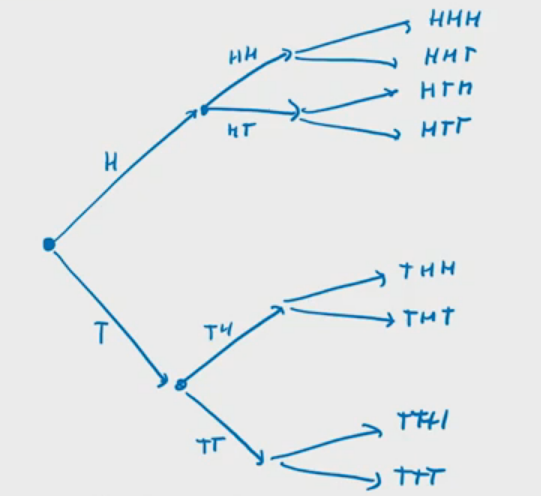
\includegraphics[width=0.5\linewidth,keepaspectratio]{math1}
\end{center}

\tiny{(Ref: Math for Machine Learning - AWS Brent Werness)}

\item What we want are HHT, HTH, THH. So 3 out of 8. 
\item Probability of  this event  = 3 / 8

\end{itemize}


\end{frame}


%%%%%%%%%%%%%%%%%%%%%%%%%%%%%%%%%%%%%%%%%%%%%%%%%%%%%%%%%%
\begin{frame}{Probability} 
\begin{definition}
Given an experiment, let $S$ be the set of all possible outcomes ($S$ is often called the \underline{sample space}) and $A$ be the event of some particular outcomes (so $A\subseteq S$).  The probability of $A$, denoted by $P(A)$, is the relative proportion of $A$ in $S$.
\end{definition}

\end{frame}

%%%%%%%%%%%%%%%%%%%%%%%%%%%%%%%%%%%%%%%%%%%%%%%%%%%%%%%%%%
\begin{frame}{Probability} 
\begin{example}
Suppose we are rolling a fair die, then $S=\{1,2,3,4,5,6\}$.  Let $A$ be the event that the outcome is an even number, that is, $A=\{2,4,6\}$.  Then $P(A)= 1/2$.
\end{example}

\begin{example}
Suppose we are rolling two fair dice, and let $A$ be the event that the sum of outcomes is either 6 or 7.  Then $P(A)= 11/35$.
\end{example}
\end{frame}

%%%%%%%%%%%%%%%%%%%%%%%%%%%%%%%%%%%%%%%%%%%%%%%%%%%%%%%%%%
\begin{frame}{Some terminologies }
\begin{itemize}
\item Experiment or Trial: an action where the result is uncertain. Example: Tossing a coin, throwing dice are examples of experiments. 
\item Outcome: A single possibility from the experiment. E.g. $\Omega = {HHT, THT, \ldots}$, each of these are outcomes.
\end{itemize}
\end{frame}

%%%%%%%%%%%%%%%%%%%%%%%%%%%%%%%%%%%%%%%%%%%%%%%%%%%%%%%%%%
\begin{frame}{Event}
\begin{itemize}
\item Event: a set of outcomes/results of an experiment 
 \item An event is what we are looking for ue $E={ExactlyTwoHeads}$. E is any subset of the sample space. The set of all events associated with a given
experiment is called the event space.
\item Example Events: 
\begin{itemize}
\item Getting a Tail when tossing a coin is an event 

\item Rolling a ''5'' is an event. 
\end{itemize}
\item An event can include one or more possible outcomes: 
\begin{itemize}
\item Choosing a ''King'' from a deck of cards (any of the 4 Kings) is an 
event 
\item Rolling an ''even number'' (2, 4 or 6) is also an event 
\end{itemize}
\end{itemize}
\end{frame}

%%%%%%%%%%%%%%%%%%%%%%%%%%%%%%%%%%%%%%%%%%%%%%%%%%%%%%%%%%
\begin{frame}
\frametitle{Sample space }
\begin{itemize}
\item  
Sample Space: all the possible outcomes of an experiment. Example: choosing a card from a deck 
\begin{itemize}
\item There are 52 cards in a deck (not including Jokers) 
\item So  the  Sample  Space  is  all  52  possible  cards:  {Ace  of  Hearts,  2  of 
Hearts, etc. } 
\end{itemize}
\item A Sample Point is just one possible outcome. 
\item And an Event can be one or more of the possible outcomes. 
\item Flipping the coin:  the sample space is  $\{H,T\}$.

\item Whats the sample space of number of heads if we flip a coin 10 times?

\item $\{0,1,\ldots,10\}$

\end{itemize}
\end{frame}

%%%%%%%%%%%%%%%%%%%%%%%%%%%%%%%%%%%%%%%%%%%%%%%%%%%%%%%%%%
\begin{frame}
\frametitle{Probability of an event? }
\begin{itemize}
\item  Both `event' and `probability' are intuitively understood by most 
people, but we need to establish certain rules. 
\item  `Rain tomorrow', `3 or fewer cyclones next year', `Crop yield will 
exceed a given threshold' are  all examples of `events' whose 
`probabilities' might be of interest. 
\end{itemize}

\begin{center}
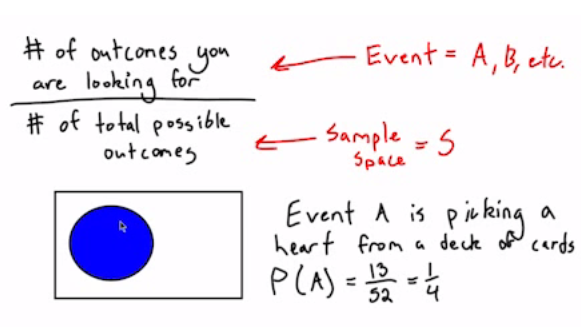
\includegraphics[width=0.65\linewidth,keepaspectratio]{evsamp}
\end{center}
\end{frame}


%%%%%%%%%%%%%%%%%%%%%%%%%%%%%%%%%%%%%%%%%%%%%%%%%%%%%%%%%%%
%\begin{frame}{Probability, continued} 
%\begin{example}
%If we choose a real number $x$ from the interval $[0,5]$, what is the probability that $2\leq x \leq 4$?  In this case, $S=[0,5]$ and $A=[2,4]$.  It follows that $P(A)= 2/5$.
%\end{example}
%
%\begin{example}
%\begin{center}
%%\includegraphics[width=3cm]{circle.png}
%\end{center}
%If we choose a point from the square above, the probability that the point belongs to the shaded region equals  $\frac{(2r)^2-\pi r^2}{(2r)^2}= 1-\frac{\pi}{4}= 0.215$.
%\end{example}
%\end{frame}

%%%%%%%%%%%%%%%%%%%%%%%%%%%%%%%%%%%%%%%%%%%%%%%%%%%%%%%%%%
\begin{frame}{Axioms* of Probability}
\begin{itemize}
\item Probability is between 0 and 1. ie $P(E) \in [0,1]$
\item Outcome is always from the sample space.
\item Summation of probabilities of all possible outcomes is 1
\end{itemize}

* Axioms are statements considered to be true without any proof.
\end{frame}



%%%%%%%%%%%%%%%%%%%%%%%%%%%%%%%%%%%%%%%%%%%%%%%%%%%%%%%%%%
\begin{frame}{Properties of Probability}
Let $S$ be the sample space and $A,B$ be events.  Then
\begin{itemize}
\item $P(S)=1, P(\emptyset)=0$. 
\item If $A\subseteq B$, then $P(A)\leq P(B)$.  In particular, $0\leq P(A)\leq 1$. 
\item $P(A\cup B)=P(A)+P(B)-P(A\cap B)$.  In particular, if $A$ and $B$ are disjoint, then $P(A
\cup B)=P(A)+P(B)$. 
\item $P(A^c)=1-P(A)$.
\end{itemize}
\end{frame}


%%%%%%%%%%%%%%%%%%%%%%%%%%%%%%%%%%%%%%%%%%%%%%%%%%%%%%%%%%
\begin{frame}
\frametitle{Visualizing Probability}
\begin{itemize}
\item  Let rectangular region being of entire sample space. Area is ``1''.
\item Points are outcomes
\item Events are collection of outcomes, so sub-regions.
\item Probability is shown as area of the sub-region.
\end{itemize}

\begin{center}
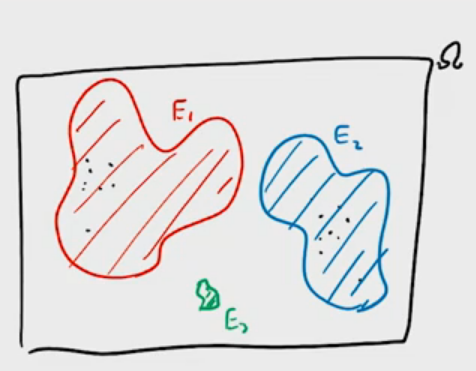
\includegraphics[width=0.5\linewidth,keepaspectratio]{math2}
\end{center}

\tiny{(Ref: Math for Machine Learning - AWS Brent Werness)}
\end{frame}

%%%%%%%%%%%%%%%%%%%%%%%%%%%%%%%%%%%%%%%%%%%%%%%%%%%%%%%%%%
\begin{frame}
\frametitle{Visualizing Probability}
\begin{itemize}
\item  Union of Events is sum of probability when they are Exclusive.
\item If they are not, meaning there is some intersection between events, then total probability is sum of both minus the intersection (as it got included twice)
\item For 3 events summation, add all 3, minus 3 double overlaps, plus add single triple overlap.
\end{itemize}

\begin{center}
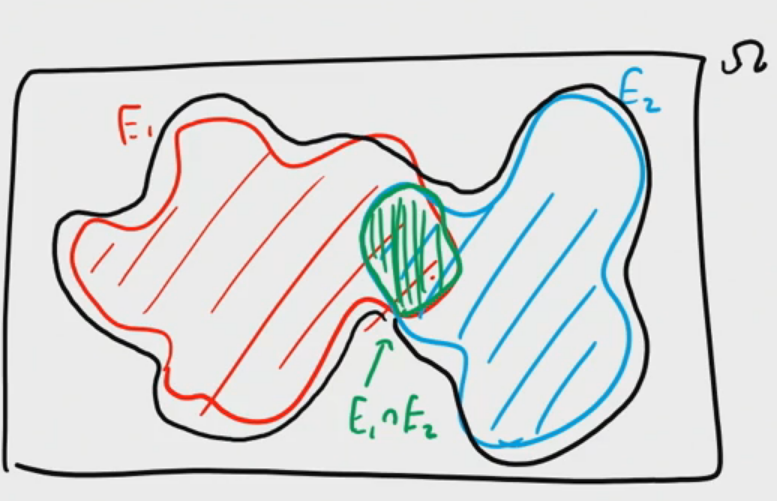
\includegraphics[width=0.5\linewidth,keepaspectratio]{math3}
\end{center}

\tiny{(Ref: Math for Machine Learning - AWS Brent Werness)}
\end{frame}



%%%%%%%%%%%%%%%%%%%%%%%%%%%%%%%%%%%%%%%%%%%%%%%%%%%%%%%%%%%%%%%%%%%%%%%%%%%%%%%%%%
\begin{frame}[fragile]\frametitle{}
\begin{center}
{\Large Probability of multiple variables}
\end{center}
\end{frame}

%%%%%%%%%%%%%%%%%%%%%%%%%%%%%%%%%%%%%%%%%%%%%%%%%%%%%%%%%%
\begin{frame}
\frametitle{Joint Probability}
\begin{itemize}
\item  To denote the probability of multiple variables AT THE SAME TIME.
\item Say, two variables, gender and hair-length.  $P(male, short)$ is the probability that a person is male and has short hair.
\end{itemize}
\end{frame}

%%%%%%%%%%%%%%%%%%%%%%%%%%%%%%%%%%%%%%%%%%%%%%%%%%%%%%%%%%
\begin{frame}
\frametitle{Conditional Probability}
\begin{itemize}
\item  To denote the probability of one event AFTER THE OTHER HAS OCCURED.
\item  $P (long hair | male)$ is the probability of having long hair given that a person is male.
\end{itemize}
\end{frame}

%%%%%%%%%%%%%%%%%%%%%%%%%%%%%%%%%%%%%%%%%%%%%%%%%%%%%%%%%%
\begin{frame}
\frametitle{Marginal Probability}
\begin{itemize}
\item  To denote the probability of one event IRRESPECTIVE OF OTHER EVENTS.
\item  Probability of person being male is given by $P(male)$. It doesn't matter whether or not the person has short hair or long.
\end{itemize}
\end{frame}

%%%%%%%%%%%%%%%%%%%%%%%%%%%%%%%%%%%%%%%%%%%%%%%%%%%%%%%%%%
\begin{frame}
\frametitle{Relation between joint, conditional and marginal probabilities}


\begin{itemize}
\item  $P(A,B) = P(B|A)P(A)$
\item $P(male,long hair)=P(long hair|male) P(male)$
\item That is, probability of a person being male and having long hair =
probability of person being male times probability of having long hair
given person is male.
\item Bayes theorem is a relation between conditional and marginal probabilities of two
variables $P(A|B) = \frac{P(B|A)P(A)}{P(B)}$
\end{itemize}
\end{frame}

%%%%%%%%%%%%%%%%%%%%%%%%%%%%%%%%%%%%%%%%%%%%%%%%%%%%%%%%%%%%%%%%%%%%%%%%%%%%%%%%%%
\begin{frame}[fragile]\frametitle{}
\begin{center}
{\Large Probability Formulation}
\end{center}
\end{frame}


%%%%%%%%%%%%%%%%%%%%%%%%%%%%%%%%%%%%%%%%%%%%%%%%%%%%%%%%%%
\begin{frame}{Unions and intersections }

\begin{itemize}
\item The union of two events A and B consists of everything included in A 
or B or both. Let  
\begin{itemize}
\item A = rain tomorrow
\item  B = rain the day after tomorrow
\item C = 3 or fewer cyclones
\item D = 4 or 5 cyclones
\end{itemize}
\item Then  
\begin{itemize}
\item $A \cup B$= rain in the next 2 days
\item $C \cup D$ = 5 or fewer cyclones
\end{itemize}
\item $ P(C \cup D) = P(C) + P(D)$, because C and D  are mutually exclusive 
(they don't overlap). 
\end{itemize}
\end{frame}

%%%%%%%%%%%%%%%%%%%%%%%%%%%%%%%%%%%%%%%%%%%%%%%%%%%%%%%%%%
\begin{frame}{Unions and intersections }

\begin{itemize}
\item $P(A \cup B) \neq P(A) + P(B)$ because A and B do overlap. 
\item$ P(A \cup B) =P(A) + P(B) - P(A \cap B)$. 
\item   $P(A \cap B)$ is the intersection of A and B; it includes everything that is in 
both A and B, and is counted twice if we add P(A) and P(B). 
\end{itemize}

\begin{center}
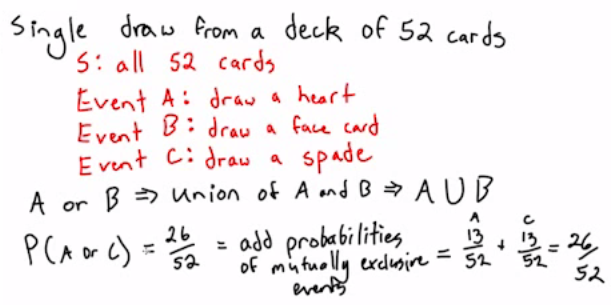
\includegraphics[width=0.65\linewidth,keepaspectratio]{undis}
\end{center}
\end{frame}

%%%%%%%%%%%%%%%%%%%%%%%%%%%%%%%%%%%%%%%%%%%%%%%%%%%%%%%%%%
\begin{frame}{Unions and intersections }
\begin{itemize}
\item In our example  
\begin{itemize}
\item $A \cap B$  = (rains tomorrow and the day after tomorrow).  
\item  $C \cap D$  is empty - it is impossible for C and D to occur 
simultaneously, so $P(C \cap D)= 0$. 
\end{itemize}

\end{itemize}
\begin{center}
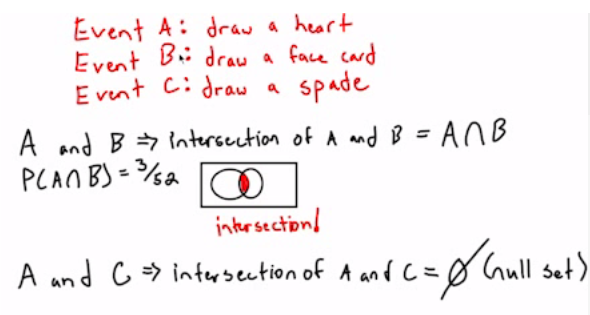
\includegraphics[width=0.65\linewidth,keepaspectratio]{intdis}
\end{center}
\end{frame}

%%%%%%%%%%%%%%%%%%%%%%%%%%%%%%%%%%%%%%%%%%%%%%%%%%%%%%%%%%
\begin{frame}{Joint Probability}

\begin{itemize}
\item Multiple events and we are trying to find chance of happening all of them together
\item So? Intersection set of all events
\item  If A and C are independent, $P(A \cup C) = P(A)P(C)$. 
%\item  If A and C are dependent, $P(A \cup C) = P(A)P(C)$. 
\end{itemize}
\end{frame}



%%%%%%%%%%%%%%%%%%%%%%%%%%%%%%%%%%%%%%%%%%%%%%%%%%%%%%%%%%
\begin{frame}{Independence }

\begin{itemize}
\item Two events are independent, if the occurrence of one does not affect the probability of occurrence of the other.
\item Similarly, two random variables are independent if the realization of one does not affect the
probability distribution of the other.
\item Example: rolling dice. First outcome, does not influence second outcome at all.
\item In pack of cards: pick a card and then pick a card again, are independent if the first card is put back.
\end{itemize}
\end{frame}

%%%%%%%%%%%%%%%%%%%%%%%%%%%%%%%%%%%%%%%%%%%%%%%%%%%%%%%%%%
\begin{frame}{Independence }
\begin{itemize}
\item In dice example  
\begin{itemize}
\item $A$  = getting 3  
\item  $B$ = getting 6
\item  $C$ = getting even number
\end{itemize}
\item Total outcome of 2 events, $6x6$ pairs of possible outcomes, e.g. 1-1, 1-2,1-3 \ldots, 6-6.
\item $P(A \cap B) = P(A)P(B) = 1/6 \times 1/6 = 1/36$. 
\item $P(A \cap C) = P(A)P(C) = 1/6 \times 3/6 = 3/36$. 
\item {\bf NOTE: A and C are not outcome of same event, which would have been NULL. They are two separate events, one after another, thus there is non-zero probability}
\end{itemize}
\end{frame}


%%%%%%%%%%%%%%%%%%%%%%%%%%%%%%%%%%%%%%%%%%%%%%%%%%%%%%%%%%
\begin{frame}{Without replacement? }
\begin{itemize}
\item First pair pulled is black
\item Second pair getting black without putting the first one back.
\item These are Dependent events. So answer is not pure multiplication, but with some adjustment.
\item Conditional Probability is for Dependent probabilities
\end{itemize}
\begin{center}
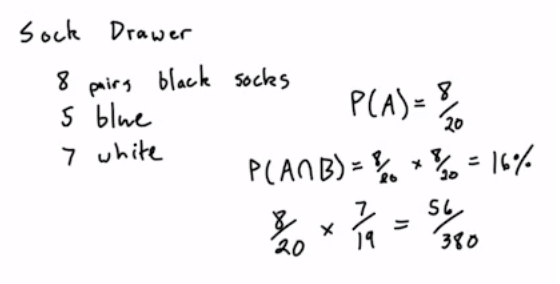
\includegraphics[width=0.65\linewidth,keepaspectratio]{socks}
\end{center}
\end{frame}

%%%%%%%%%%%%%%%%%%%%%%%%%%%%%%%%%%%%%%%%%%%%%%%%%%%%%%%%%%
\begin{frame}{Conditional probability }
\begin{center}
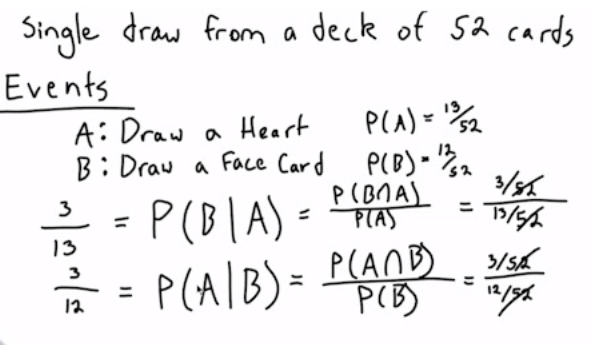
\includegraphics[width=0.5\linewidth,keepaspectratio]{condprob1}
\end{center}
\begin{itemize}
\item Calculate probabilities of A and B, independently.
\item but then if I say, that the first card is Heart, then whats the probability of Face Card.
\item There are 13 hearts. Among hearts there are 3 face cards. So, 3 /13. 3 face-heart cards, total 13 hearts.
\item reverse, first face, then whats prbability of getting heart. So, 12 face cards and 3 out of them are hearts. So, 3/12.
\end{itemize}
\end{frame}


%%%%%%%%%%%%%%%%%%%%%%%%%%%%%%%%%%%%%%%%%%%%%%%%%%%%%%%%%
\begin{frame}{ Conditional probability}

\begin{itemize}
\item  If we know that one event has occurred it may change our view of the 
probability of another event. Let  
\item  A = {rain today}, B = {rain tomorrow}.  
\item  It is likely that knowledge that A has occurred will change your view 
of the probability that B will occur. 
\item  We write $P(B|A) \neq P(B), P(B|A) = P(A \cap B)/P(A)$ denotes the 
conditional probability of B, given A.  
\end{itemize}
\begin{center}
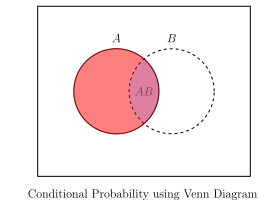
\includegraphics[width=0.3\linewidth,keepaspectratio]{condprob}
\end{center}

\end{frame}
%%%%%%%%%%%%%%%%%%%%%%%%%%%%%%%%%%%%%%%%%%%%%%%%%%%%%%%%%%
\begin{frame}

\begin{center}
\begin{tabular}{|l|l|l|l|l|}
\hline
&	A	&B	&C&	Total\\
\hline
Male&	8&	18&	13&	39\\
\hline
Female&	10	&4	&12&	26\\
\hline
Total&	18&	22&	25&	65\\
\hline
\end{tabular}
\end{center}
If one student was chosen at random, find the probability that the student got an A given that he is male.\\

\vspace{.1in}
$P(\hbox{A}|\hbox{male})=  \frac{8}{39}$  \\
\vspace{.1in}
Find the probability that a student is male given that he got an A.\\
\vspace{.1in} 
$P(\hbox{male}|\hbox{A}) =  \frac{8}{18}$ 
\end{frame}

%%%%%%%%%%%%%%%%%%%%%%%%%%%%%%%%%%%%%%%%%%%%%%%%%%%%%%%%%%
\begin{frame}
\frametitle{Conditional Probability Formula}
If events A and B are not independent, then $P(A\hbox{ and }B) = P(A) \cdot P(B | A)$.



If you pull 2 cards out of a deck, what is the probability that both are twos?\\ 
\vspace{.1in}
The probability that the first card is a two is  $\frac{4}{52}$.\\ 
\vspace{.1in}
The probability that the second card is a two, given that the first was a two, is  $\frac{3}{51}$.\\ 
\vspace{.1in}
The probability that both cards are twos is  $\frac{4}{52}\cdot \frac{3}{51}=\frac{12}{2652}\simeq 0.00452$.

\end{frame}


%%%%%%%%%%%%%%%%%%%%%%%%%%%%%%%%%%%%%%%%%%%%%%%%%%%%%%%%%%
%\begin{frame}{ Conditional probability}
%
%\begin{itemize}
%\item  Simplistically, it is just ratio of who purchased output who clicked.
%\end{itemize}
%\begin{center}
%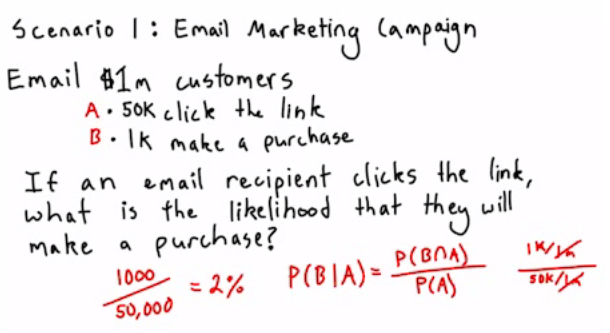
\includegraphics[width=0.5\linewidth,keepaspectratio]{condprob2}
%\end{center}
%
%%%%%%%%%%%%%%%%%%%%%%%%%%%%%%%%%%%%%%%%%%%%%%%%%%%%%%%%%
\begin{frame}{ Graphical Conditional Probability}

\begin{center}
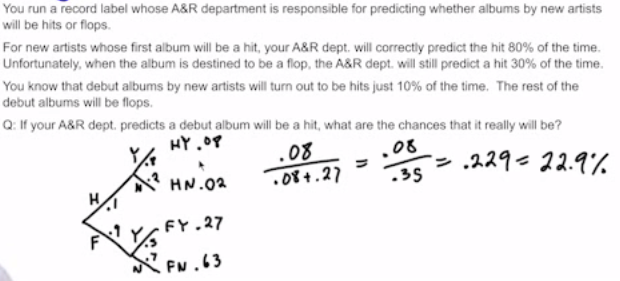
\includegraphics[width=\linewidth,keepaspectratio]{bayes1}
\end{center}
\end{frame}

%%%%%%%%%%%%%%%%%%%%%%%%%%%%%%%%%%%%%%%%%%%%%%%%%%%%%%%%%%%%%%%%%%%%%%%%%%%%%%%%%%
\begin{frame}[fragile]\frametitle{}
\begin{center}
{\Large Probability vs Likelihood}
\end{center}
\end{frame}

%%%%%%%%%%%%%%%%%%%%%%%%%%%%%%%%%%%%%%%%%%%%%%%%%%%%%%%%%%%%%%%%%%%%%%%%
\begin{frame}[fragile]\frametitle{Probability}
Lets look at Normal distribution, even though this applies for all types of distributions.


	\begin{itemize}
	\item Say, we are plotting weights (on x), frequencies on y.
	\item Probability that someones weight will be tween 32 and 34 is the area under that curve. 0.29
	\item There is 29\% chance that a randomly selected observation will have weight between 32 to 34.
	\end{itemize}

      \begin{center}
      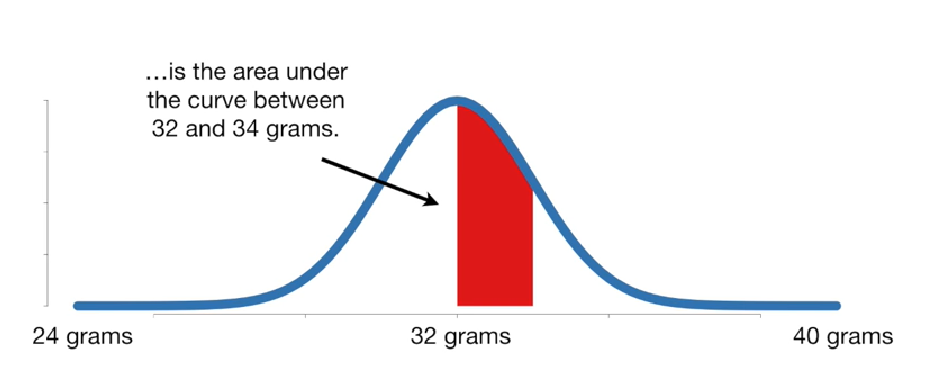
\includegraphics[width=0.8\linewidth,keepaspectratio]{statq42}
	  
	  
	  	\end{center}
		
		
\tiny{(Ref: StatQuest: Probability vs Likelihood- Josh Starmer )}

\end{frame}

%%%%%%%%%%%%%%%%%%%%%%%%%%%%%%%%%%%%%%%%%%%%%%%%%%%%%%%%%%%%%%%%%%%%%%%%
\begin{frame}[fragile]\frametitle{Likelihood}
Lets look at only one observation, say 34 grams.


	\begin{itemize}
	\item The Likelihood of the observation to have 34 is the point on this curve. 0.12
	\item If we had shifted the distribution to match mean of 32, the Likelihood would be 0.21
	\item So, Likelihoods are the y axis values for fixed data points with distributions that can be moved.
	\end{itemize}

      \begin{center}
      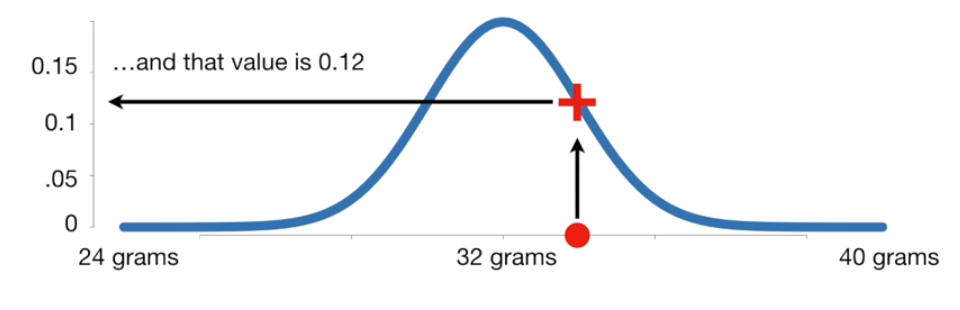
\includegraphics[width=0.5\linewidth,keepaspectratio]{statq43}
	  
	        \includegraphics[width=0.5\linewidth,keepaspectratio]{statq44}
	  
	  	\end{center}

		\tiny{(Ref: StatQuest: Probability vs Likelihood- Josh Starmer )}

\end{frame}

%%%%%%%%%%%%%%%%%%%%%%%%%%%%%%%%%%%%%%%%%%%%%%%%%%%%%%%%%%%%%%%%%%%%%%%%
\begin{frame}[fragile]\frametitle{Summary}


      \begin{center}
      \includegraphics[width=\linewidth,keepaspectratio]{statq45}
	  
	  
	  	\end{center}

		\tiny{(Ref: StatQuest: Probability vs Likelihood- Josh Starmer )}

\end{frame}

%%%%%%%%%%%%%%%%%%%%%%%%%%%%%%%%%%%%%%%%%%%%%%%%%%%%%%%%%%%%%%%%%%%%%%%%%%%%%%%%%%
\begin{frame}[fragile]\frametitle{}
\begin{center}
{\Large Maximum Likelihood}
\end{center}
\end{frame}

%%%%%%%%%%%%%%%%%%%%%%%%%%%%%%%%%%%%%%%%%%%%%%%%%%%%%%%%%%%%%%%%%%%%%%%%
\begin{frame}[fragile]\frametitle{Maximum Likelihood}
Lets say we are measuring weights \ldots

	\begin{itemize}
	\item The goal of Maximum Likelihood is to find the optimal way to fit a distribution to the data.
	\item Is the shown Normal distribution fitting the data? It is not.
	\item Likelihood of observations is away from the center of the distribution.
	\end{itemize}

      \begin{center}
      \includegraphics[width=0.8\linewidth,keepaspectratio]{statq46}
	  
	  	\end{center}

		\tiny{(Ref: StatQuest: Maximum Likelihood, clearly explained!!! - Josh Starmer )}

\end{frame}

%%%%%%%%%%%%%%%%%%%%%%%%%%%%%%%%%%%%%%%%%%%%%%%%%%%%%%%%%%%%%%%%%%%%%%%%
\begin{frame}[fragile]\frametitle{Maximum Likelihood}
What if we shift the normal distribution on right so that the mean was the same as the average weight?

	\begin{itemize}
	\item The goal of Maximum Likelihood is to find the optimal way to fit a distribution to the data.
	\item Is the shown Normal distribution fitting the data? It is not.
	\item Likelihood of observations is away from the center of the distribution. Looks good.
	\item If we had shifted too much on the right, not good, again.
	\end{itemize}

      \begin{center}
      \includegraphics[width=0.6\linewidth,keepaspectratio]{statq47}
	  
	  	\end{center}

		\tiny{(Ref: StatQuest: Maximum Likelihood, clearly explained!!! - Josh Starmer )}

\end{frame}

%%%%%%%%%%%%%%%%%%%%%%%%%%%%%%%%%%%%%%%%%%%%%%%%%%%%%%%%%%%%%%%%%%%%%%%%
\begin{frame}[fragile]\frametitle{Maximum Likelihood}
We plot all the possible shifting positions and find the best!!


      \begin{center}
      \includegraphics[width=0.8\linewidth,keepaspectratio]{statq48}
	  
	  	\end{center}

		\tiny{(Ref: StatQuest: Maximum Likelihood, clearly explained!!! - Josh Starmer )}

\end{frame}

%%%%%%%%%%%%%%%%%%%%%%%%%%%%%%%%%%%%%%%%%%%%%%%%%%%%%%%%%%%%%%%%%%%%%%%%
\begin{frame}[fragile]\frametitle{Maximum Likelihood}
Results:

      \begin{center}
      \includegraphics[width=0.8\linewidth,keepaspectratio]{statq50}
	  
	  	\end{center}

		\tiny{(Ref: StatQuest: Maximum Likelihood, clearly explained!!! - Josh Starmer )}

\end{frame}


%%%%%%%%%%%%%%%%%%%%%%%%%%%%%%%%%%%%%%%%%%%%%%%%%%%%%%%%%%%%%%%%%%%%%%%%%%%%%%%%%%
\begin{frame}[fragile]\frametitle{}
\begin{center}
{\Large Bayes Theorem Example}
\end{center}
\end{frame}


%%%%%%%%%%%%%%%%%%%%%%%%%%%%%%%%%%%%%%%%%%%%%%%%%%%%%%%%%%
\begin{frame}{Bayes Theorem  Example }

\begin{itemize}
\item  Suppose that $0.8\%$ of the general population has a certain disease, and suppose that we have a test for it.
\item The test says so $90\%$ of the time. 
\item If a person does not have the disease, the test gives a false diagnosis $7\%$ of the time. 
\item When a particular patient tests positive, what is the probability they have the disease?
\end{itemize}
\end{frame}

%%%%%%%%%%%%%%%%%%%%%%%%%%%%%%%%%%%%%%%%%%%%%%%%%%%%%%%%%%
\begin{frame}{Bayes Theorem  Example }

\begin{itemize}
\item   Let $D$ be the event that the person has the disease and $\bar{D}$ be its complement;
\item let $Y$ (for ``yes'') be the event that the test \emph{says} the person has the disease, with complement $\bar{Y}$.
\end{itemize}
\begin{eqnarray*}
	P(D)       &=& 0.008 \\
	P(Y|D)     &=& 0.90 \\
	P(Y|D\bar) &=& 0.07.
\end{eqnarray*}
\end{frame}

%%%%%%%%%%%%%%%%%%%%%%%%%%%%%%%%%%%%%%%%%%%%%%%%%%%%%%%%%%
\begin{frame}{Bayes Theorem  Example }

Let's find the probability
of $Y$ by itself.  Using the partition theorem we know this is
\begin{eqnarray*}
	P(Y) &=& P(Y|D)\,P(D) \;+\; P(Y|\bar{D})\,P(\bar{D}) \\
	&=& 0.90 \cdot 0.008 + 0.07\cdot 0.992 \\
	&=& 0.077.
\end{eqnarray*}
So the non-conditional probabilities are
\begin{align*}
	P(\bar{D})  &= 0.992  & P(\bar{Y})  &= 0.923 \\
	P(D)      &= 0.008  & P(Y)      &= 0.077.
\end{align*}
\end{frame}

%%%%%%%%%%%%%%%%%%%%%%%%%%%%%%%%%%%%%%%%%%%%%%%%%%%%%%%%%%
\begin{frame}{Bayes Theorem  Example }

\begin{itemize}
\item   Looking at $D$ and $Y$ separately, 
\item We can think of the population at large as
being split into those with and without the disease, and those for whom the
test is positive or negative.  
\item Suppose in particular that we have a sample of
1000 people who are representative of the general population. 
\end{itemize}
\end{frame}


%%%%%%%%%%%%%%%%%%%%%%%%%%%%%%%%%%%%%%%%%%%%%%%%%%%%%%%%%%
\begin{frame}{Bayes Theorem  Example }
Here are some
(very rectangular) Venn diagrams:
$$
%
	\begin{tabular}{|c|c||c|}
	\hline $\bar{D}$ & $D$ & \\
	\hline
	&&\\
	$992$ & $8$ & \\
	&&\\
	\hline
	\end{tabular}
%
	\qquad
	\qquad
%
	\begin{tabular}{|ccc||c|}
	\hline $\;$ & $\;$ & $\;$ & $\;$ \\
	\hline
	\hline  & &923& $\bar{Y}$ \\
	\hline  & & 77& $Y$ \\
	\hline
	\end{tabular}
%
$$
\end{frame}

%%%%%%%%%%%%%%%%%%%%%%%%%%%%%%%%%%%%%%%%%%%%%%%%%%%%%%%%%%
\begin{frame}{Bayes Theorem  Example }
Bayes' theorem has to do with how these two partitions intersect to make four
groups:
% $$
	\begin{tabular}{|r|r||c|}
	\hline $\bar{D}$ & $D$ & \\
	\hline
	\hline  $P(\bar{Y}|\bar{D}) \cdot 992 = ?$ & $P(\bar{Y}|D) \cdot 8 = ?$ & $\bar{Y}$ \\
	\hline  $P(Y    |\bar{D}) \cdot 992 = ?$ & $P(Y    |D) \cdot 8 = ?$ & $Y$ \\
	\hline
	\end{tabular}
%
	\qquad
	
	
	\textrm{and}
	
	
	\qquad
	
%
	\begin{tabular}{|r|r||c|}
	\hline $\bar{D}$ & $D$ & \\
	\hline
	\hline  $P(\bar{D}|\bar{Y}) \cdot 923 = ?$ & $P(D|\bar{Y}) \cdot 923 = ?$ & $\bar{Y}$ \\
	\hline  $P(\bar{D}|Y)     \cdot  77 = ?$ & $P(D|Y)     \cdot  77 = ?$ & $Y$ \\
	\hline
	\end{tabular}
% $$
\end{frame}




%%%%%%%%%%%%%%%%%%%%%%%%%%%%%%%%%%%%%%%%%%%%%%%%%%%%%%%%%%
\begin{frame}{Bayes Theorem  Example }
We can use the theorem to find the probability our patient has the
disease, given the positive test result:
\begin{eqnarray*}
	P(D|Y) &=& P(Y|D) \; \frac{P(D)}{P(Y)} \\
	&=& 0.90 \;\cdot\; \frac{0.008}{0.077} \\
	&=& 0.094.
\end{eqnarray*}
That is, there's only a one-in-eleven chance the patient actually has the
disease.
\end{frame}

%%%%%%%%%%%%%%%%%%%%%%%%%%%%%%%%%%%%%%%%%%%%%%%%%%%%%%%%%%
\begin{frame}{Bayes Theorem  Example }
We have two conditional probabilities given:  $P(Y|D)$ and $P(Y|\bar{D})$.  We
found $P(D|Y)$.  What about $P(D|\bar{Y})$?  We can use the  partition theorem
(theorem \ref{thm:partition}) again to solve for what we don't know in terms of
what we do know:
\begin{eqnarray*}
	P(D) &=& P(D|Y)\,P(Y) \;+\; P(D|\bar{Y})\,P(\bar{Y}) \\
	P(D|\bar{Y}) &=& \frac{P(D) - P(D|Y)\,P(Y)}{P(\bar{Y})} \\
	&=& \frac{0.008 - 0.094 \cdot 0.077}{0.923} \\
	&=& 0.0008.
\end{eqnarray*}
We now have all four conditional probabilities:
\begin{align*}
	P(Y|\bar{D}) &= 0.07  & P(D|\bar{Y}) &= 0.0008 \\
	P(Y|D)     &= 0.90  & P(D|Y)     &= 0.094.
\end{align*}
\end{frame}

%%%%%%%%%%%%%%%%%%%%%%%%%%%%%%%%%%%%%%%%%%%%%%%%%%%%%%%%%%
\begin{frame}{Bayes Theorem  Example }
Now we can fill out the four-square table:
\begin{itemize}

\item Since $P(Y|\bar{D})=0.07$, seven percent of the 992 disease-free people (70
of them) get false positives; the rest (922) get a correct negative result.

%These are the people in the left-hand column of the four-square table.

\item Since $P(Y|D)=0.90$, ninety percent of the 8 people with the disease test
positive (i.e. all but one of them); one of the 8 gets a false sense of security.

\item Since $P(D|\bar{Y})=0.0008$, $0.08\%$ of the 923 with negative test results
(one person) does in fact have the disease; the other 922 (as we found just above)
get a correct negative result.

\item Since $P(D|Y)=0.094$, only $9.4\%$ of the 77 people with positive test
results (7 people) have the disease; the other 70 get a scare (and, presumably,
a re-test).

\end{itemize}
\end{frame}

%%%%%%%%%%%%%%%%%%%%%%%%%%%%%%%%%%%%%%%%%%%%%%%%%%%%%%%%%%
\begin{frame}{Bayes Theorem  Example }
So, the sample of 1000 people splits up as follows:
$$
	\begin{tabular}{|r|r|c|}
	\hline $\bar{D}$ & $D$ & \\
	$922$ & $1$ & $\bar{Y}$ \\
	\hline  $70$ & $7$ & $Y$ \\
	\hline
	\end{tabular}
%
$$
Moreover, we can rank events by likelihood:
\begin{itemize}
\item[(1)] Healthy people correctly diagnosed: $92.2\%$.
\item[(2)] False positives: $7\%$.
\item[(3)] People with the disease, correctly diagnosed: $0.7\%$.
\item[(4)] False negatives: $0.1\%$.
\end{itemize}

Now it's no surprise our patient got a false positive:  this happens 10 times
as often as a correct positive diagnosis.
\end{frame}


% %%%%%%%%%%%%%%%%%%%%%%%%%%%%%%%%%%%%%%%%%%%%%%%%%%%%%%%%%%
% \begin{frame}
% \frametitle{Bayes Theorem}

% $P(\hbox{disease}|\hbox{positive})$\\
% \vspace{0.1in}


% \begin{equation*}=\frac{P(\hbox{disease})P(\hbox{positive}|\hbox{disease})}{P(\hbox{disease})P(\hbox{positive}|\hbox{disease})+P(\hbox{no disease})P(\hbox{positive}|\hbox{no disease})}\end{equation*}\\
% \vspace{.1in}

% \begin{equation*}
% =\frac{(0.05)(.92)}{(0.05)(0.92)+(0.95)(0.03)} \simeq 0.617\end{equation*}
% \end{frame}


%%%%%%%%%%%%%%%%%%%%%%%%%%%%%%%%%%%%%%%%%%%%%%%%%%%%%%%%%%%%
%%\begin{frame}{Bayes Theorem  Expanded}
%%
%%\begin{theorem} Let $A_1, A_2,\ldots,A_n$  be a set of mutually exclusive events that together  
%%form the sample space S. Let B be any event from the same sample space,  
%%such that $P(B) > 0$. Then, 
%%$$ P(A_k|B) = \frac{P(A_k \cap B)}{P(A_1 \cap B) + P(A_2 \cap B) + \ldots + P(A_n \cap B)}$$
%%$$ P(A_k|B) = \frac{P(A_k) P(B|A_k)}{P(A_1)P(B| \cap A_1) + \ldots + P(A_n)P( B|A_n)}$$
%%\end{theorem}
%%Note: The denominator in above equations is P(B).
%%\end{frame}
%%
%%%%%%%%%%%%%%%%%%%%%%%%%%%%%%%%%%%%%%%%%%%%%%%%%%%%%%%%%%%%
%%\begin{frame}{Bayes Theorem: Example  }
%% If a randomly selected lamp is defective, what is the probability that the 
%% lamp was manufactured in factory A3? 
%%\begin{center}
%%\includegraphics[width=0.8\linewidth,keepaspectratio]{bays1}
%%\end{center}
%%\end{frame}
%%
%%%%%%%%%%%%%%%%%%%%%%%%%%%%%%%%%%%%%%%%%%%%%%%%%%%%%%%%%%%%
%%\begin{frame}{Bayes Theorem: Example  }
%%\begin{center}
%%\includegraphics[width=0.8\linewidth,keepaspectratio]{bays2}
%%\end{center}
%%There is 40.67\% chance that, a defective product found is produced  
%%in Factory A3. 
%%\end{frame}
%%
%%%%%%%%%%%%%%%%%%%%%%%%%%%%%%%%%%%%%%%%%%%%%%%%%%%%%%%%%%
\begin{frame}{Comparisions}
\begin{itemize}\setlength{\itemsep}{0.3cm}

\item Classical statistics: model parameters are \emph{fixed} and \emph{unknown}.

\item A Bayesian thinks of parameters as random, and thus having distributions (just like the data). We can thus think about unknowns for which no reliable frequentist experiment exists, e.g. $\theta =$ proportion of US men with untreated prostate cancer.
		
\item A Bayesian writes down a \emph{prior} guess for parameter(s) $\theta$, say $p(\theta)$. He then combines this with the information provided by the observed data $by$ to obtain the \emph{posterior} distribution of $\theta$, which we denote by $p(\theta given by)$.

\item All statistical inferences (point and interval estimates, hypothesis tests) then follow from posterior summaries. For example, the posterior means/medians/modes offer point estimates of $\theta$, while the quantiles yield credible intervals.

\end{itemize}
\end{frame}

%%%%%%%%%%%%%%%%%%%%%%%%%%%%%%%%%%%%%%%%%%%%%%%%%%%%%%%%%%
\begin{frame}

\begin{itemize}\setlength{\itemsep}{0.5cm}
 \item The key to Bayesian inference is ``learning'' or ``updating'' of prior beliefs. Thus, posterior information $\geq$ prior information.

 \item Is the classical approach wrong? That may be a controversial statement, but it certainly is fair to say that the classical approach is limited in scope.

 \item The Bayesian approach expands the class of models and easily handles:
	\begin{itemize}
	\item repeated measures
	\item unbalanced or missing data
	\item nonhomogenous variances
	\item multivariate data
	\end{itemize}	
	-- and many other settings that are precluded (or much more complicated) in classical settings.
\end{itemize}

\end{frame}

%%%%%%%%%%%%%%%%%%%%%%%%%%%%%%%%%%%%%%%%%%%%%%%%%%%%%%%%%%%%%%%%%%%%%%%%%%%%%%%%%%
\begin{frame}[fragile]\frametitle{}
\begin{center}
{\Large Random Variables}
\end{center}
\end{frame}

%%%%%%%%%%%%%%%%%%%%%%%%%%%%%%%%%%%%%%%%%%%%%%%%%%%%%%%%%%
\begin{frame}\frametitle{Random Variables}
\begin{itemize}
\item Those variables which can take different value randomly are called
random variables.
\item If the variables are discrete in nature, they are called discrete random
variables.
\item Similarly, if the variables are continuous in nature, then it is called
continuous random variable.
\end{itemize}
\end{frame}



%%%%%%%%%%%%%%%%%%%%%%%%%%%%%%%%%%%%%%%%%%%%%%%%%%%%%%%%%%
\begin{frame} \frametitle{Random variables}
A {\bf random variable} is generated by a ``random'' function. 

Types:
\begin{itemize}
\item Nominal
\item Ordinal
\item Quantitative
\end{itemize}
\end{frame}


%%%%%%%%%%%%%%%%%%%%%%%%%%%%%%%%%%%%%%%%%%%%%%%%%%%%%%%%%%
\begin{frame}\frametitle{Nominal Random Variable}
\begin{itemize}
\item A {\bf nominal} random variable, also called {\bf qualitative} or {\bf  categorical}, takes on values in a set of names or labels.
\item Examples of nominal sample spaces include geographical locations, biological species, and ethnic categories.
\item Data from a nominal random variable cannot be {\bf strictly ordered}.
\end{itemize}
\end{frame}

%%%%%%%%%%%%%%%%%%%%%%%%%%%%%%%%%%%%%%%%%%%%%%%%%%%%%%%%%%
\begin{frame}\frametitle{Ordinal Random Variable}

\begin{itemize}
\item An {\bf ordinal} measurement is usually either a {\bf ranking}
($1^{\rm st}$, $2^{\rm nd}$, etc.) or a {\bf rating} (good, bad,
favorable, strongly agree, etc.).  

\item Ordinal values can be ordered, but do not have {\bf measurement units}
\item It doesn't always make sense to subtract or divide their numerical
values.
\end{itemize}
\end{frame}

%%%%%%%%%%%%%%%%%%%%%%%%%%%%%%%%%%%%%%%%%%%%%%%%%%%%%%%%%%
\begin{frame}\frametitle{Quantitative Random Variable}

\begin{itemize}
\item A {\bf quantitative} random variable represents a magnitude, for
example the result of counting something, or the result of measuring a
physical quantity such as length, width, or volume.

\item Quantitative measurements can always be ordered.
\end{itemize}
\end{frame}

%%%%%%%%%%%%%%%%%%%%%%%%%%%%%%%%%%%%%%%%%%%%%%%%%%%%%%%%%%%
%\begin{frame}
%\frametitle{Measurement scales}
%
%\begin{itemize}
%\item Celsius temperature is an interval scale -- it makes
%perfect sense to compare two temperatures by subtracting them.
%\item Is Celsius temperature a ratio scale?  Is the coffee twice as hot as
%the tea?
%\item 
%The answer is no.  The freezing point of water defines the origin of
%the Celsius scale.  This is arbitrary.  Pure ethanol freezes at
%$-114^\circ$C, so if we used the freezing point of ethanol as the zero
%point of the scale, the ratio between the two objects' temperatures
%would be only $(50+114)/(25+114)=1.2$.
%
%\textcolor{blue}{Note:} There is some ambiguity and controversy about
%these designations.
%
%\end{frame}

%%%%%%%%%%%%%%%%%%%%%%%%%%%%%%%%%%%%%%%%%%%%%%%%%%%%%%%%%%%
\begin{frame}
\frametitle{ Quantitative Random Variable }
Types:
\begin{itemize}
\item Discrete: Number of days that it rains yearly 
\item Continuous:  Amount of rain on a given day 
\end{itemize}
Note that these designations aren't used in the case of nominal or
ordinal random variables.
\end{frame}

%%%%%%%%%%%%%%%%%%%%%%%%%%%%%%%%%%%%%%%%%%%%%%%%%%%%%%%%%%%
\begin{frame}
\frametitle{ Quantitative Random Variable }

\begin{itemize}
\item A {\bf discrete} random variable takes on finitely many values, or
infinitely many separated values (e.g.\ $0,1,2,\ldots$).

\item A {\bf continuous} random variable can take on any real number in some
interval (e.g.\ $[0,1]$ or $[0,\infty)$).  

\item Gray area between discrete and continuous random variables:
e.g.\ monetary values recorded in dollars or dollars and cents
\end{itemize}
\end{frame}

%%%%%%%%%%%%%%%%%%%%%%%%%%%%%%%%%%%%%%%%%%%%%%%%%%%%%%%%%%%
\begin{frame}
\frametitle{Units, populations and samples}

\begin{itemize}
\item A {\bf unit} (more specifically {\bf ``sampling unit''}) is one member
of the collection.
\item A {\bf population} is the set of all units of interest. 
\item In practice, we cannot observe the whole population, so we usually
work with a {\bf sample} of units
\end{itemize}
\end{frame}

%%%%%%%%%%%%%%%%%%%%%%%%%%%%%%%%%%%%%%%%%%%%%%%%%%%%%%%%%%%
\begin{frame}
\frametitle{Units, populations and samples}

%\textcolor{blue}{\bf Example:} Suppose we are interested in childrens'
%diets, and we sample 100 seven year old
%girls in the US and record their food intake for one day.

\begin{itemize}
\item Properties of a sample will generally differ from properties of the
population.  
\item For example, the 100 children in our sample may have
somewhat higher or somewhat lower average calorie intake than the
population at large. 
\item 
Statistics: how samples relate to
populations, and what we can confidently state about a population
given the limited information in a sample.

\end{itemize}

\end{frame}

%%%%%%%%%%%%%%%%%%%%%%%%%%%%%%%%%%%%%%%%%%%%%%%%%%%%%%%%%%
\begin{frame}\frametitle{Random Variables}
\begin{itemize}
\item  Random variable can take on randomly different
value. 
\item But are all the values that it takes can be equal or likely be equal
too, or is it more likely that the random variable take a particular value
more often than other?
\item Depends on the way (function) using which random numbers are generated.
\end{itemize}
\end{frame}

%%%%%%%%%%%%%%%%%%%%%%%%%%%%%%%%%%%%%%%%%%%%%%%%%%%%%%%%%%
\begin{frame}\frametitle{Random Variable Generation}
\begin{itemize}
\item  Experiment: records numbers from a SINGLE six face die.
\item X axis shows 6 possible outcomes.
\item Y axis shows their probabilities.
\item For each of the 6 possible values on X axis, the Y value is same ie 1/6
\item Uniform distribution
\end{itemize}
\end{frame}

%%%%%%%%%%%%%%%%%%%%%%%%%%%%%%%%%%%%%%%%%%%%%%%%%%%%%%%%%%
\begin{frame}\frametitle{Random Variable Generation}
\begin{itemize}
\item  Experiment: records sum of numbers from TWO six face dies.
\item X axis shows 12 possible outcomes.
\item Y axis shows their probabilities.
\item For each of the 12 possible values on X axis, the Y value is NOT SAME.
\end{itemize}

\begin{center}
\includegraphics[width=0.5\linewidth,keepaspectratio]{pmf}
\end{center}
\end{frame}

%%%%%%%%%%%%%%%%%%%%%%%%%%%%%%%%%%%%%%%%%%%%%%%%%%%%%%%%%%
\begin{frame}\frametitle{Random Variable Generation}
\begin{itemize}
\item  If the random variable is discrete in nature, we use Probability Mass
Function to describe its probability distribution
\item If the random variable is continuous in nature, we use Probability
Density Function to describe its probability distribution.
\end{itemize}
\end{frame}

%%%%%%%%%%%%%%%%%%%%%%%%%%%%%%%%%%%%%%%%%%%%%%%%%%%%%%%%%%%
\begin{frame}
\frametitle{Probability distributions}
The probability distribution for a random variable X gives the possible 
values for X, and the probabilities associated with each possible value 
(i.e., the likelihood that the values will occur). 
Types:
\begin{itemize}
\item Discrete probability distributions 
\item Continuous probability distributions 
\end{itemize}
\end{frame}

%%%%%%%%%%%%%%%%%%%%%%%%%%%%%%%%%%%%%%%%%%%%%%%%%%%%%%%%%%%
\begin{frame}
\frametitle{Discrete Probabilities}

\begin{itemize}
\item If a random variable has a discrete sample space, a probability
distribution is just a listing of the probabilities with which each
point in the sample space occurs.  
\item These probabilities must sum to 1.
\end{itemize}
\end{frame}


%%%%%%%%%%%%%%%%%%%%%%%%%%%%%%%%%%%%%%%%%%%%%%%%%%%%%%%%%%%
\begin{frame}
\frametitle{Example: Discrete Probabilities}

\begin{itemize}
\item Survey of a political candidate.  

\begin{center}
\begin{tabular}{ll}
{$x$} & {$P(X=x)$}\\\hline Favorable & \hspace{0.8cm}0.3 \\ Neutral
& \hspace{0.8cm}0.5 \\ Unfavorable & \hspace{0.8cm}0.2 \\\hline
\end{tabular}
\end{center}

\item
The mapping from points in a discrete sample space to the
corresponding probabilities is called a {\bf probability mass function
  (PMF)}.
\item
The sample space is finite.
\end{itemize}
\end{frame}

%%%%%%%%%%%%%%%%%%%%%%%%%%%%%%%%%%%%%%%%%%%%%%%%%%%%%%%%%%%
\begin{frame}
\frametitle{Many Discrete Probabilities}

\begin{itemize}
\item Infinitely many
rows

\begin{center}
\begin{tabular}{ll}
{$x$} & {$P(X=x)$}\\\hline 
0 & \hspace{0.8cm}0.37\\
1 & \hspace{0.8cm}0.37\\
2 & \hspace{0.8cm}0.18\\
3 & \hspace{0.8cm}0.06\\
$\cdots$ & \hspace{0.8cm}$\cdots$
\end{tabular}
\end{center}
\item 
Although there are infinitely many nonzero probabilities, they still
must sum to one.
\end{itemize}
\end{frame}
%
%
%%%%%%%%%%%%%%%%%%%%%%%%%%%%%%%%%%%%%%%%%%%%%%%%%%%%%%%%%%%%
%\begin{frame}
%\frametitle{Example: Many Discrete Probabilities}
%
%\begin{itemize}
%\item Suppose we flip a coin repeatedly until
%we get the first tail, and count the number of heads that we see
%before the tail occurs.  
%\item The sample space is $\{0,1,2,\ldots\}$ -- it
%is infinite.
%\end{itemize}
%\end{frame}

%%%%%%%%%%%%%%%%%%%%%%%%%%%%%%%%%%%%%%%%%%%%%%%%%%%%%%%%%%%
\begin{frame}
\frametitle{Probability Mass Function }

\begin{itemize}
\item function that generates discrete variables with probabilities
\item $f(x_i) = P(X=x_i)$ is the probability that $X$ has the value $x_i$.
\item Properties:
\begin{itemize}
\item $0\leq f(x_i)\leq1 $
\item $\sum f(x_i) =f(x_1) +f(x_2) + \ldots = 1$ 
\end{itemize}
\end{itemize}
\end{frame}

%%%%%%%%%%%%%%%%%%%%%%%%%%%%%%%%%%%%%%%%%%%%%%%%%%%%%%%%%%%
\begin{frame}
\frametitle{Example: Probability Mass Function }

\begin{itemize}
\item Suppose the random variable X is the number of rooms in a 
randomly chosen owner-occupied housing unit. 
\item The distribution of X is: 

\begin{center}
\includegraphics[width=0.8\linewidth,keepaspectratio]{rooms}
\end{center}
\end{itemize}

\end{frame}


%%%%%%%%%%%%%%%%%%%%%%%%%%%%%%%%%%%%%%%%%%%%%%%%%%%%%%%%%%%
\begin{frame}
\frametitle{Probability Density Function }

\begin{itemize}
\item function that generates continous random variables with probabilities
\item $f(x_{(a,b)}) = P(X=x_{(a,b)})$ is the probability that $X$ has the values in range $(a,b)$.
\item Properties:
\begin{itemize}
\item $0\leq f(x_i)\leq1 $
\item $\int f(x_i) = 1$ 
\end{itemize}
\end{itemize}
\end{frame}

%%%%%%%%%%%%%%%%%%%%%%%%%%%%%%%%%%%%%%%%%%%%%%%%%%%%%%%%%%%%
\begin{frame}
\frametitle{Distributions of continuous random variables}

Two important identities are

\begin{center}
\begin{tabular}{ccc}
$P(X>x)$ &=& $1 - P(X \le x)$\\ $P(a < X \le b)$ &=& $P(X\le b) -
  P(X < a)$.
\end{tabular}
\end{center}

Therefore we only need to know $P(X \le x)$ for all values of $x$ and
we can determine the probability that $X$ lies in any given interval.

{\bf Its area under curve}
\end{frame}

%%%%%%%%%%%%%%%%%%%%%%%%%%%%%%%%%%%%%%%%%%%%%%%%%%%%%%%%%%%%
\begin{frame}
\frametitle{Distributions of continuous random variables}

\textcolor{blue}{\bf Example:} Suppose we want to know the probability
that a person in a certain population is between 170cm and 180cm tall.
If we know that the probability of being less than 180cm tall is
$0.8$, and the probability of being less than 170cm tall is $0.6$,
then the probability of being between 170cm and 180cm tall is
$0.8-0.6=0.2$.

To put this in mathematical notation, let $X$ denote the height of a
randomly selected person from the population.  Then 

$$ P(170<X\le 180) = P(X\le 180) - P(X<170) = 0.8-0.6.
$$

\end{frame}

%%%%%%%%%%%%%%%%%%%%%%%%%%%%%%%%%%%%%%%%%%%%%%%%%%%%%%%%%%%
\begin{frame}
\frametitle{Density functions}

The distribution of a continuous random variable is described by a
{\bf density function}.  

A density function is a non-negative function such that the area
between the horizontal axis and the function is exactly 1.

The orange curves below are density functions.  The grey area on the
left is $P(X \le -0.5)$, which is 0.31 for this distribution.  The
grey area on the right is $P(X \le 2.5)$, which is 0.92 for this
distribution.


\begin{center}
\begin{tabular}{cc}
\scalebox{0.4}{\includegraphics{000.pdf}} &
\scalebox{0.4}{\includegraphics{001.pdf}}
\end{tabular}
\end{center}

\end{frame}

%%%%%%%%%%%%%%%%%%%%%%%%%%%%%%%%%%%%%%%%%%%%%%%%%%%%%%%%%%%
\begin{frame}
\frametitle{Characteristics of density functions}

A basic property of a density function is its {\bf location} -- the
central or most typical value.  

There are many measures of location, but by any reasonable measure the
density on the right, below, would have a greater location than the
density on the left.

\begin{center}
\begin{tabular}{cc}
\scalebox{0.4}{\includegraphics{002-0.pdf}}&
\scalebox{0.4}{\includegraphics{002-1.pdf}}
\end{tabular}
\end{center}

\end{frame}

%%%%%%%%%%%%%%%%%%%%%%%%%%%%%%%%%%%%%%%%%%%%%%%%%%%%%%%%%%%
\begin{frame}
\frametitle{Characteristics of density functions}

Another basic property of a density function is its {\bf scale},
referring to spread or width of the distribution.  

There are many measures of scale, but by any reasonable measure the
density on the right, below, would have a greater scale than the
density on the left.

\begin{center}
\begin{tabular}{cc}
\scalebox{0.4}{\includegraphics{002-2.pdf}}&
\scalebox{0.4}{\includegraphics{002-3.pdf}}
\end{tabular}
\end{center}


\end{frame}

%%%%%%%%%%%%%%%%%%%%%%%%%%%%%%%%%%%%%%%%%%%%%%%%%%%%%%%%%%%
\begin{frame}
\frametitle{Characteristics of density functions}

Another basic property of a density function is its {\bf skew},
referring to whether one of the two tails of the density is thicker
than the other.  

The density on the left, below, is right-skewed, and the density on
the right, below, is left-skewed.


\begin{center}
\begin{tabular}{cc}
\scalebox{0.4}{\includegraphics{002-4.pdf}}&
\scalebox{0.4}{\includegraphics{002-5.pdf}}
\end{tabular}
\end{center}

%The densities on the preceding two slides are unskewed, or symmetric.

\end{frame}


%%%%%%%%%%%%%%%%%%%%%%%%%%%%%%%%%%%%%%%%%%%%%%%%%%%%%%%%%%%
\begin{frame}
\frametitle{Discrete Probability Distributions }
Some examples:
\begin{itemize}
\item Bernoulli distribution :$ P(X = 1) = p,           P(X = 0) = 1- p$
 
\item Binomial distribution : -Two possible outcomes, probability constant = $(\frac{n}{x})p^x (1-p)^{n-x}$
 
\item Poisson distribution 
 
\item Negative Binomial 
\end{itemize}
\end{frame}

%%%%%%%%%%%%%%%%%%%%%%%%%%%%%%%%%%%%%%%%%%%%%%%%%%%%%%%%%%
\begin{frame}{Bernoulli}

Bernoulli random variable is used when the experiment results in
either success or failure where success is represented as 1 and failure as
0. If P is probability of success, then probability mass function of
Bernoulli variable x is given as:

\begin{center}
\includegraphics[width=0.45\linewidth,keepaspectratio]{bernoulli}
\end{center}
\end{frame}

%%%%%%%%%%%%%%%%%%%%%%%%%%%%%%%%%%%%%%%%%%%%%%%%%%%%%%%%%%
\begin{frame}{Binomial}

Binomial distribution is used when we want to count how many success we
have when we repeat an experiment for n numbers of time
independently. The probability mass function of binomial variable x,
where p is probability of success, is given as:

\begin{center}
\includegraphics[width=0.45\linewidth,keepaspectratio]{binom}
\end{center}
\end{frame}

%%%%%%%%%%%%%%%%%%%%%%%%%%%%%%%%%%%%%%%%%%%%%%%%%%%%%%%%%%
\begin{frame}{Poisson}

Poisson variable x is used when we are counting the number of
occurrences of an event in a unit of time such that the occurrences are
independent and rarely simultaneous. For an average number of
occurrence $\lambda$ the probability mass function is given as:
\begin{center}
\includegraphics[width=0.45\linewidth,keepaspectratio]{poisson}
\end{center}
\end{frame}


%%%%%%%%%%%%%%%%%%%%%%%%%%%%%%%%%%%%%%%%%%%%%%%%%%%%%%%%%%%
\begin{frame}
\frametitle{Continuous Probability Distributions }
Some examples:
\begin{itemize}
\item  Normal distribution 
 
\item  Uniform distribution 
 
\item  Exponential distribution 
 
\item  Weibull distribution 
 
\end{itemize}
\end{frame}

%%%%%%%%%%%%%%%%%%%%%%%%%%%%%%%%%%%%%%%%%%%%%%%%%%%%%%%%%%
\begin{frame}{Normal}

Normal random variable x comes handy for different situations. We can
use it to model physical measurements like weight, height etc. We can
also use it to model error made by measuring instruments. In general, it
can be used when the average and variance of the quantity being
measured is known. The probability density function is given as:
\begin{center}
\includegraphics[width=0.65\linewidth,keepaspectratio]{normdist1}
\end{center}
\end{frame}

%%%%%%%%%%%%%%%%%%%%%%%%%%%%%%%%%%%%%%%%%%%%%%%%%%%%%%%%%%
\begin{frame}{Uniform}

We use uniform random variable x when the probability density for
every value between an interval (starting from a and ending at b) is
equal. The probability density function of x is given as:
\begin{center}
\includegraphics[width=0.65\linewidth,keepaspectratio]{uniform}
\end{center}
\end{frame}

%%%%%%%%%%%%%%%%%%%%%%%%%%%%%%%%%%%%%%%%%%%%%%%%%%%%%%%%%%
\begin{frame}{Exponential}

Exponential variable x are used when we are measuring the time until
the  rst occurrence of an event, such that the occurrences in disjoint
time intervals are independent and rarely simultaneous. For the
average number of occurrences per unit time a, the probability density
function is given as:
\begin{center}
\includegraphics[width=0.65\linewidth,keepaspectratio]{expo}
\end{center}
\end{frame}

%%%%%%%%%%%%%%%%%%%%%%%%%%%%%%%%%%%%%%%%%%%%%%%%%%%%%%%%%%%
\begin{frame}
\frametitle{Event probabilities}

An {\bf event} is a set of one or more points in the sample space.
The probability of an event is the sum of the probabilities for the
points in the event.

\textcolor{blue}{\bf Example:} Consider this distribution:

\begin{center}
\begin{tabular}{ll}
{$x$} & {$P(X=x)$}\\\hline 
Favorable & \hspace{0.8cm}0.3 \\
Neutral & \hspace{0.8cm}0.5 \\
Unfavorable & \hspace{0.8cm}0.2 \\\hline
\end{tabular}
\end{center}

The response being either \textcolor{purple}{favorable or neutral} is
an event, and this event has probability $0.3+0.5=0.8$.

\end{frame}

%%%%%%%%%%%%%%%%%%%%%%%%%%%%%%%%%%%%%%%%%%%%%%%%%%%%%%%%%%%
\begin{frame}
\frametitle{Cumulative probabilities}

If the sample space is ordered, then the probability of observing a
value less than or equal to a given number $x$ is the {\bf cumulative
  probability at $x$}.

\textcolor{blue}{\bf Example:} If we are interested in the probability
distribution of the number of times a person living in Michigan has
visited Florida, we might have the following probabilities and
cumulative probabilities:

\begin{center}
\begin{tabular}{lllllllll}
$x$         & 0   & 1 & 2 & 3 & 4 & 5 & $\cdots$\\\hline
$P(X=x)$    & 0.3 & 0.1 & 0.2 & 0.1 & 0.06 & 0.08 & $\cdots$\\
$P(X\le x)$ & 0.3 & 0.4 & 0.6 & 0.7 & 0.76 & 0.84 & $\cdots$\\\hline
\end{tabular}
\end{center}

\end{frame}

%%%%%%%%%%%%%%%%%%%%%%%%%%%%%%%%%%%%%%%%%%%%%%%%%%%%%%%%%%%%
%\begin{frame}
%\frametitle{Exercises}
%
%The following distribution describes the number of times a 20 year-old
%male visits a doctor in a year.  Some of the probabilities are not
%shown.
%
%\begin{center}
%\begin{tabular}{lllll}
%$x$         & 0   & 1 & 2 & 3+ \\\hline
%$P(X=x)$    & 0.55 & ? & 0.1 & ?\\
%\end{tabular}
%\end{center}
%
%\begin{itemize}
%
%\item What is the range of possible values for the probability that
%  exactly one visit to the doctor occurs?
%
%\item What are the largest and smallest possible values for the
%  cumulative probability at 1?
%
%\item What are the largest and smallest possible values for the
%  probability that the person visits the doctor at least
%  once?
%
%\end{itemize}
%
%\end{frame}

%%%%%%%%%%%%%%%%%%%%%%%%%%%%%%%%%%%%%%%%%%%%%%%%%%%%%%%%%%%
\begin{frame}
\frametitle{Independence}

Two random variables are {\bf independent} if the probability that
both of them satisfy some condition at the same time is the product of
the probabilities of the conditions being satisfied separately.

For example,

$$
P(X=2\;{\rm and}\;Y=3) = P(X=2)\cdot P(Y=3)
$$

\begin{center}
$P(0\le X<1\;{\rm and}\;Y>4) = P(0 \le X < 1)\cdot P(Y>4)$ 
\end{center}

\end{frame}

%%%%%%%%%%%%%%%%%%%%%%%%%%%%%%%%%%%%%%%%%%%%%%%%%%%%%%%%%%%
\begin{frame}
\frametitle{Example: Independence}

\begin{itemize}
\item College students at an educational institution where 52\% of the
students are female,
\item 40\% of the students visit a doctor at
least once a year.

\item the probability
that a randomly selected student is female and has visited a doctor in
the last year is?

\item  $0.52\times 0.4 = 0.208$.

\item Corollary: if the value sis not $0.208$ then these variables
are {\bf dependent}.
\end{itemize}
\end{frame}

%%%%%%%%%%%%%%%%%%%%%%%%%%%%%%%%%%%%%%%%%%%%%%%%%%%%%%%%%%%
\begin{frame}
\frametitle{Independence}
\begin{itemize}

\item If the proportion is greater than 0.208, the variables are {\bf
  positively dependent}.

\item If the proportion is less than 0.208, the variables are {\bf
  negatively dependent}.

\end{itemize}

\end{frame}
%
%%%%%%%%%%%%%%%%%%%%%%%%%%%%%%%%%%%%%%%%%%%%%%%%%%%%%%%%%%%%
%\begin{frame}
%\frametitle{Independence}
%
%\textcolor{blue}{\bf Example:} suppose we are interested in the
%relationship between a person's income at age 30 (denoted $I$), and
%the number of siblings they have (denoted $S$).  If these two random
%variables are independent, then
%
%\begin{eqnarray*}
%P(I=\$45,000\;{\rm and}\; S=1) &=& P(I=\$45,000)\times P(S=1)\\
%P(I=\$55,000\;{\rm and}\; S=2) &=& P(I=\$55,000)\times P(S=2)
%\end{eqnarray*}
%
%The multiplication property holds for all events, not just events
%consisting of a single outcome.  If $I$ and $S$ are independent, then
%
%\begin{eqnarray*}
%\lefteqn{P(\$35,000 \le I \le \$55,000\; {\rm and}\; S\le 1) =}\\ 
%&&P(\$35,000 \le I \le \$55,000)\times P(S\le 1).
%\end{eqnarray*}
%
%\end{frame}

%%%%%%%%%%%%%%%%%%%%%%%%%%%%%%%%%%%%%%%%%%%%%%%%%%%%%%%%%%%%
\begin{frame}
\frametitle{Complements}

\begin{itemize}

\item For a particular event $E$, there is a related event denoted $E^c$
which is the event that $E$ does not happen.

\item Example: $E$ may be that the person who answers is female.  
\item The complementary
event would be the event that the person who answers is male.

\item The probability of the complement of an event is 1 minus the
probability of the event: $P(E^c) = 1 - P(E)$.
\end{itemize}


\end{frame}

%%%%%%%%%%%%%%%%%%%%%%%%%%%%%%%%%%%%%%%%%%%%%%%%%%%%%%%%%%%%
\begin{frame}
\frametitle{Complements}
\textcolor{blue}{\bf Example:} If the probability that a person
living in Michigan has visited Florida at most two times is 0.6, the
complementary event is that the person has visited Florida three or
more times, and the probability of this event is 0.4.
\begin{center}
\begin{tabular}{cc}
\scalebox{0.4}{\includegraphics{039-1.pdf}}&
\scalebox{0.4}{\includegraphics{039-2.pdf}}
\end{tabular}
\end{center}

\end{frame}

%%%%%%%%%%%%%%%%%%%%%%%%%%%%%%%%%%%%%%%%%%%%%%%%%%%%%%%%%%%%
\begin{frame}
\frametitle{Disjoint events}

Two events are {\bf disjoint} if they contain no points in common.
These two events are disjoint:

\begin{center}
\begin{tabular}{ll}
E1:& A person's birthday is on the 31st day of the month\\
E2:& A person's birthday is in June
\end{tabular}
\end{center}

\end{frame}

%%%%%%%%%%%%%%%%%%%%%%%%%%%%%%%%%%%%%%%%%%%%%%%%%%%%%%%%%%%%
\begin{frame}
\frametitle{Disjoint events}

But these events are not disjoint:

\begin{center}
\begin{tabular}{ll}
E1:& A person's birthday is on a Tuesday\\
E2:& A person's birthday is in June
\end{tabular}
\end{center}

\end{frame}

%%%%%%%%%%%%%%%%%%%%%%%%%%%%%%%%%%%%%%%%%%%%%%%%%%%%%%%%%%%%
\begin{frame}
\frametitle{Disjoint events}

Events $E1$ and $E2$ are disjoint on the left, but not on the
right. The large gray circle represents the full sample space.

\begin{center}
\begin{tabular}{cc}
\scalebox{0.4}{\includegraphics{040-1.pdf}}&
\scalebox{0.4}{\includegraphics{040-2.pdf}}
\end{tabular}
\end{center}

\end{frame}


%%%%%%%%%%%%%%%%%%%%%%%%%%%%%%%%%%%%%%%%%%%%%%%%%%%%%%%%%%%%
\begin{frame}
\frametitle{Disjoint events}

If events $E1$ and $E2$ are disjoint, then the probability of at least
one of them happening is the sum of their probabilities:

$$
P(E1\;{\rm or}\;E2) = P(E1) + P(E2).
$$
\end{frame}

%%%%%%%%%%%%%%%%%%%%%%%%%%%%%%%%%%%%%%%%%%%%%%%%%%%%%%%%%%%%
\begin{frame}
\frametitle{Example: Disjoint events}
Roll a fair die, and consider these events:

\begin{center}
\begin{tabular}{ll}
E1:& The result is even\\
E2:& The result is a 3 or a 5
\end{tabular}
\end{center}

The event ``$E1$ or $E2$'' is the event that I get a 2, 3, 4, 5, or 6.
This event has probability $5/6$.  Since $P(E1) = 1/2$ and $P(E2) =
1/3$, we can check that $P(E1\;{\rm or}\;E2) = 5/6 = 1/2 + 1/3 = P(E1)
+ P(E2)$.

\end{frame}

%%%%%%%%%%%%%%%%%%%%%%%%%%%%%%%%%%%%%%%%%%%%%%%%%%%%%%%%%%%%
\begin{frame}
\frametitle{Disjoint events}

Now consider these events:

\begin{center}
\begin{tabular}{ll}
E1:& The result is even\\
E2:& The result is less than or equal to 3
\end{tabular}
\end{center}

These events are not disjoint, since 2 is in both events.

The event ``$E1$ or $E2$'' is the event that I get a 1, 2, 3, 4, or 6.
This event has probability $5/6$.  But $P(E1) = 1/2$ and $P(E2) = 1/2$
so $P(E1)+P(E2) \ne P(E1\;{\rm or}\;E2)$.

\end{frame}

%%%%%%%%%%%%%%%%%%%%%%%%%%%%%%%%%%%%%%%%%%%%%%%%%%%%%%%%%%%%
\begin{frame}
\frametitle{Exercises}

Suppose we are considering a population of students that is 52\%
female, and for which 40\% of the students have visited a doctor in
the last year.

\begin{itemize}

\item If these events are independent, what is the probability that a
  randomly sampled student is a male who has not seen a doctor in the
  last year?

\item If these events are independent, what is the probability that a
  randomly sampled student is either a male who has not seen a doctor
  in the last year, or is a female who has not seen a doctor in the
  last year?

\item If there are 1000 students in our population, and gender is
  independent of whether a student visited a doctor in the past year,
  how many students are females who have not seen a doctor in the past
  year?

\end{itemize}

\end{frame}

%%%%%%%%%%%%%%%%%%%%%%%%%%%%%%%%%%%%%%%%%%%%%%%%%%%%%%%%%%%%
\begin{frame}
\frametitle{Answers}


\begin{itemize}

\item $P(Student=Male) = 0.48$, and $P(StudentNoSeenDoctorLastYear) = 0.6$ (both are complements of the events given in the exercise).  By
  independence, $P(Student=Male,And,StudentNoSeenDoctorLastYear) = 0.48*0.6 = 0.288$.

\item Simalalry $P(Student=Female,And,StudentNoSeenDoctorLastYear) = 0.52*0.6 =
  0.312$.  These events are disjoint, so the probability of one or the
  other occuring is 0.288+0.312 = 0.6.  It's not a coincidence that
  this is equal to 1-0.4, the probability of visiting a doctor
  regardless of gender.

\item The probability that a student is a female who has not seen a
  doctor in the last year is 0.312, so the number of such people is
  1000*0.312 = 312.

\end{itemize}

\end{frame}

%%%%%%%%%%%%%%%%%%%%%%%%%%%%%%%%%%%%%%%%%%%%%%%%%%%%%%%%%%%%%%
%%\begin{frame}
%%\frametitle{Distributions of continuous random variables}
%%
%%\begin{itemize}
%%
%%\item For a continuous random variable, $P(X=x)=0$ for all $x$.  
%%
%%\item It takes on values in an interval, for example
%%
%%$$
%%P(X\le 3),\; P(X>-1),\; P(2 < X \le 3).
%%$$
%%
%%\end{itemize}
%%\end{frame}




% \section[Stats]{Statistics}
% %%%%%%%%%%%%%%%%%%%%%%%%%%%%%%%%%%%%%%%%%%%%%%%%%%%%%%%%%%%%%%%%%%%%%%%%%%%%%%%%%%
\begin{frame}[fragile]\frametitle{}
\begin{center}
{\Large Statistics}
\end{center}
\end{frame}




% %%%%%%%%%%%%%%%%%%%%%%%%%%%%%%%%%%%%%%%%%%%%%%%%%%%%%%%%%%%%%%%%%%%%%%%%%%%%%%%%%%
\begin{frame}[fragile]\frametitle{}
\begin{center}
{\Large Descriptive Statistics}
\end{center}
\end{frame}


%%%%%%%%%%%%%%%%%%%%%%%%%%%%%%%%%%%%%%%%%%%%%%%%%%%%%%%%%%%
\begin{frame}[fragile]\frametitle{Descriptive Statistics}
\begin{itemize}
\item Describes the data characteristics
\item To make sense of the data
\item To make rational decisions
\item E.g. Demographics, clinical data.
\item Measures of Central Tendencies
\item Measures of Variability
\item Measures of Shape
\end{itemize}
\end{frame}

%%%%%%%%%%%%%%%%%%%%%%%%%%%%%%%%%%%%%%%%%%%%%%%%%%%%%%%%%%%
\begin{frame}[fragile]\frametitle{Why Descriptive Statistics?}
\begin{itemize}
\item Population: the whole
\item Sample: small subset of the population
\item Gauging Population by examining traits of Sample.
\item Example Question: Finding height of Americans?
\item Not going to measure everyone height, but that in a {\bf representative} sample.
\item Example: Election sampling?
\end{itemize}
\end{frame}



%%%%%%%%%%%%%%%%%%%%%%%%%%%%%%%%%%%%%%%%%%%%%%%%%%%%%%%%%%%
\begin{frame}[fragile]\frametitle{Why Descriptive Statistics?}
\begin{itemize}
\item To check the accuracy and precision of the process
\item To reduce variability and improve process capability
\item To know the truth about the real world
\end{itemize}
\end{frame}


%%%%%%%%%%%%%%%%%%%%%%%%%%%%%%%%%%%%%%%%%%%%%%%%%%%%%%%%%%%%%%%%%%%%%%%%%%%%%%%%%%
\begin{frame}[fragile]\frametitle{}
\begin{center}
{\Large Basic Terms}
\end{center}
\end{frame}

%%%%%%%%%%%%%%%%%%%%%%%%%%%%%%%%%%%%%%%%%%%%%%%%%%%%%%%%%%%%%%%%%%%%%%%%
\begin{frame}[fragile]\frametitle{Histogram}

\begin{columns}
    \begin{column}[T]{0.6\linewidth}
Example
	\begin{itemize}
	\item Say, we are measuring height of people.
	\item Plotting them on X axis.
	\item The dots would look very crowded where there are many close or repetitive observations.
	\item Some dots get hidden.
	\item We can improve the visualization, by plotting frequency (number of occurrences) on Y axis.
	\item But in case of contiguous variable, like, exact measurements are rare. So we `bin' them and measure occurrences.
	\item Thats Histogram.
	\end{itemize}

    \end{column}
    \begin{column}[T]{0.4\linewidth}
      \begin{center}
      \includegraphics[width=\linewidth,keepaspectratio]{statq1}
	  
	  \includegraphics[width=\linewidth,keepaspectratio]{statq2}
	  
	  \includegraphics[width=\linewidth,keepaspectratio]{statq3}	  
	  	\end{center}
    \end{column}

  \end{columns}
  

\tiny{(Ref: StatQuest: What is a Histogram? - Josh Starmer )}
\end{frame}

%%%%%%%%%%%%%%%%%%%%%%%%%%%%%%%%%%%%%%%%%%%%%%%%%%%%%%%%%%%%%%%%%%%%%%%%
\begin{frame}[fragile]\frametitle{Histogram}

\begin{columns}
    \begin{column}[T]{0.6\linewidth}

	\begin{itemize}
	\item Histogram can be used to predict probability of getting (future) measurements.
	\item Getting measurement (as shown in the box) in the middle region is more likely.
	\item Measurements at both the ends are rare.
	\item We can approximate this histogram of observations by a `distribution'.
	\item Looks like `Normal' distribution, or a bell-curve
	\end{itemize}

    \end{column}
    \begin{column}[T]{0.4\linewidth}
      \begin{center}
      \includegraphics[width=\linewidth,keepaspectratio]{statq4}
	  
	  \includegraphics[width=\linewidth,keepaspectratio]{statq5}
	  
	  \includegraphics[width=\linewidth,keepaspectratio]{statq6}	  
	  	\end{center}
    \end{column}

  \end{columns}
  

\tiny{(Ref: StatQuest: What is a Histogram? - Josh Starmer )}
\end{frame}

%%%%%%%%%%%%%%%%%%%%%%%%%%%%%%%%%%%%%%%%%%%%%%%%%%%%%%%%%%%%%%%%%%%%%%%%
\begin{frame}[fragile]\frametitle{Histogram}

\begin{columns}
    \begin{column}[T]{0.6\linewidth}

	\begin{itemize}
	\item If the frequency of measurements seem decreasing, it may be an exponential distribution.
	\item Binning criterion is critical. They can not be too narrow or too wide.
	\item Try different bin widths/formulas to plot a histogram.
	\end{itemize}

    \end{column}
    \begin{column}[T]{0.4\linewidth}
      \begin{center}
      \includegraphics[width=\linewidth,keepaspectratio]{statq7}
	  
	  \includegraphics[width=\linewidth,keepaspectratio]{statq8}
	  
	  \includegraphics[width=\linewidth,keepaspectratio]{statq9}	  
	  	\end{center}
    \end{column}

  \end{columns}
  

\tiny{(Ref: StatQuest: What is a Histogram? - Josh Starmer )}
\end{frame}


%%%%%%%%%%%%%%%%%%%%%%%%%%%%%%%%%%%%%%%%%%%%%%%%%%%%%%%%%%%%%%%%%%%%%%%%%%%%%%%%%%
\begin{frame}[fragile]\frametitle{}
\begin{center}
{\Large Descriptive Statistics Example}
\end{center}
\end{frame}


%%%%%%%%%%%%%%%%%%%%%%%%%%%%%%%%%%%%%%%%%%%%%%%%%%%%%%%%%%%
\begin{frame}[fragile]\frametitle{Descriptive Statistics}
\begin{itemize}
\item Describes features of data sets using numbers
\item Individual row: Data
\item Full table: Dataset
\item Purpose: Answer questions.
\end{itemize}
\begin{center}
\includegraphics[width=0.35\linewidth,keepaspectratio]{da1}
\end{center}
\end{frame}

%%%%%%%%%%%%%%%%%%%%%%%%%%%%%%%%%%%%%%%%%%%%%%%%%%%%%%%%%%%
\begin{frame}[fragile]\frametitle{Questions}
\begin{center}
\includegraphics[width=0.35\linewidth,keepaspectratio]{da1}
\end{center}
\begin{itemize}
\item What is Bobby's score?
\item Out of? (Total \# entries)
\item Highest/Lowest scores?
\end{itemize}
\end{frame}

%%%%%%%%%%%%%%%%%%%%%%%%%%%%%%%%%%%%%%%%%%%%%%%%%%%%%%%%%%%
\begin{frame}[fragile]\frametitle{Questions}
\begin{center}
\includegraphics[width=0.35\linewidth,keepaspectratio]{da1}
\end{center}
\begin{itemize}
\item Class average?
\item Most Common/frequent Score?
\item Any other questions?
\end{itemize}
\end{frame}

%%%%%%%%%%%%%%%%%%%%%%%%%%%%%%%%%%%%%%%%%%%%%%%%%%%%%%%%%%%
\begin{frame}[fragile]\frametitle{Numerical Measures}
\begin{itemize}
\item Highest to Lowest Score: RANGE
\item Most Common Score: MODE
\item Average Score: MEAN
\item Any other measures?
\end{itemize}
\end{frame}

%%%%%%%%%%%%%%%%%%%%%%%%%%%%%%%%%%%%%%%%%%%%%%%%%%%%%%%%%%%
\begin{frame}[fragile]\frametitle{Descriptive Statistics}
\begin{itemize}
\item Examines ALL data (not sample)
\item Cannot generalize to other datasets
\end{itemize}
\end{frame}

%%%%%%%%%%%%%%%%%%%%%%%%%%%%%%%%%%%%%%%%%%%%%%%%%%%%%%%%%%%%%%%%%%%%%%%%%%%%%%%%%%
\begin{frame}[fragile]\frametitle{}
\begin{center}
{\Large Descriptive Statistics Example}
\end{center}
\end{frame}


%%%%%%%%%%%%%%%%%%%%%%%%%%%%%%%%%%%%%%%%%%%%%%%%%%%
\begin{frame}[fragile] \frametitle{Descriptive Tasks}

\adjustbox{valign=t}{
\begin{minipage}{0.45\linewidth}
\begin{center}
\includegraphics[width=\linewidth,keepaspectratio]{descriptivetable}
\end{center}
\end{minipage}
}
\hfill
\adjustbox{valign=t}{
\begin{minipage}{0.45\linewidth}
\begin{itemize}
\item Objective: Derive patterns, summarize underlying relationships
\item More exploratory of current state
\end{itemize}
\end{minipage}
}

\end{frame}



%%%%%%%%%%%%%%%%%%%%%%%%%%%%%%%%%%%%%%%%%%%%%%%%%%%%%%%%%%
\begin{frame}[fragile]\frametitle{Data Example}	
\begin{center}
\includegraphics[width=0.8\linewidth,keepaspectratio]{da2}
\end{center}
What sense it makes?
Any pattern?


%\code{Store as list of integers}
\end{frame}

%%%%%%%%%%%%%%%%%%%%%%%%%%%%%%%%%%%%%%%%%%%%%%%%%%%%%%%%%%
\begin{frame}[fragile]\frametitle{Visualize}	
\begin{center}
\includegraphics[width=0.8\linewidth,keepaspectratio]{da3}
\end{center}
Makes sense?


%\code{Plot the data points, not the curve}
\end{frame}

%%%%%%%%%%%%%%%%%%%%%%%%%%%%%%%%%%%%%%%%%%%%%%%%%%%%%%%%%%
\begin{frame}[fragile]\frametitle{The Shape of The Distribution}	
Better to see
\begin{center}
\includegraphics[width=0.8\linewidth,keepaspectratio]{da4}
\end{center}
Symmetric? Skewed right/left?
%\code{Plot the curve}
\end{frame}

%%%%%%%%%%%%%%%%%%%%%%%%%%%%%%%%%%%%%%%%%%%%%%%%%%%%%%%%%%%%%%%%%%%%%%%%%%%%%%%%%%
\begin{frame}[fragile]\frametitle{}
\begin{center}
{\Large Describing Data}
\end{center}
\end{frame}

%%%%%%%%%%%%%%%%%%%%%%%%%%%%%%%%%%%%%%%%%%%%%%%%%%%%%%%%%%
\begin{frame}[fragile]\frametitle{Describing Data}
\begin{itemize}
\item Univariate Analysis: Statistical moments (based on degree)
\begin{itemize}
\item 1st degree: Central tendency: mean, median, mode
\item 2nd degree: Standard Deviation: how wide data is around mean
\item 3rd degree: Skewness: Asymmetric around mean
\item 4th degree: Kurtosis: shape of skewness.
\end{itemize}
\item BiVariate Analysis: covariance, correlation
\item MultiVariate Analysis
\end{itemize}
\end{frame}


%%%%%%%%%%%%%%%%%%%%%%%%%%%%%%%%%%%%%%%%%%%%%%%%%%%%%%%%%%%
\begin{frame}[fragile]\frametitle{Univariate Analysis}
\begin{itemize}
\item Measure of Central Tendency
\item Measure of Spread
\item Measure of Asymmetry
\item Measure of Skewness
\end{itemize}
\end{frame}


%%%%%%%%%%%%%%%%%%%%%%%%%%%%%%%%%%%%%%%%%%%%%%%%%%%%%%%%%%%
%\begin{frame}[fragile]\frametitle{Frequency}	
%$ frequency(v_i) = \frac{Objects\_with\_Attribute\_v_i}{n}$
%\begin{center}
%\includegraphics[width=0.8\linewidth,keepaspectratio]{frequency}
%\end{center}
%Often used with categorical values.
%\end{frame}
%

%%%%%%%%%%%%%%%%%%%%%%%%%%%%%%%%%%%%%%%%%%%%%%%%%%%%%%%%%%%%%%%%%%%%%%%%%%%%%%%%%%
\begin{frame}[fragile]\frametitle{}
\begin{center}
{\Large Measure of Central Tendency}
\end{center}
\end{frame}

%%%%%%%%%%%%%%%%%%%%%%%%%%%%%%%%%%%%%%%%%%%%%%%%%%%%%%%%%%
\begin{frame}[fragile]\frametitle{Mean}	
\begin{itemize}
\item Measure the ``location'' of a set of values
\item Mean is a very, very common measurement
\item But is sensitive to outliers
\end{itemize}
$mean(x) = \bar{x} = 1/n \sum x_i$
%\code{Use `for' loop to calculate}
\end{frame}

%%%%%%%%%%%%%%%%%%%%%%%%%%%%%%%%%%%%%%%%%%%%%%%%%%%%%%%%%%
\begin{frame}[fragile]\frametitle{Mean}	
\begin{center}
\includegraphics[width=\linewidth,keepaspectratio]{da5}
\end{center}
Sum = 153

Mean = 153/25 = 6.12
\end{frame}

%%%%%%%%%%%%%%%%%%%%%%%%%%%%%%%%%%%%%%%%%%%%%%%%%%%%%%%%%%
\begin{frame}[fragile]\frametitle{Outliers}	
\begin{itemize}
\item Extreme data point
\item May affect calculations
\item  Can occur in any given data set and in any distribution
\item  May indicate an experimental error or incorrect recording of data
\end{itemize}
\begin{center}
\includegraphics[width=0.6\linewidth,keepaspectratio]{da15}
\end{center}
\end{frame}


%%%%%%%%%%%%%%%%%%%%%%%%%%%%%%%%%%%%%%%%%%%%%%%%%%%%%%%%%%%%%%%%%%%%%%%%
\begin{frame}[fragile]\frametitle{Mean}
Implement mean
\begin{lstlisting}
def mean(datalist):
	:
	return m

lst = [9,3,7,2,7,10,23,44,12,42,19,11,22,5,3,4,3,21,3]
result = mean(lst)
print("Mean : {}".format(result))
\end{lstlisting}
Result?
\end{frame}

%%%%%%%%%%%%%%%%%%%%%%%%%%%%%%%%%%%%%%%%%%%%%%%%%%%%%%%%%%
\begin{frame}[fragile]\frametitle{Mean}
\begin{lstlisting}
def mean(datalist):
	total = 0
	m = 0
	for item in datalist:
		total += item
	m = total / float(len(datalist))
	return m
\end{lstlisting}
Mean : 13.157894736842104
\end{frame}

%%%%%%%%%%%%%%%%%%%%%%%%%%%%%%%%%%%%%%%%%%%%%%%%%%%%%%%%%%
\begin{frame}[fragile]\frametitle{Median}	
\begin{itemize}
\item Commonly used instead of mean if outliers are present
\item Median is the middle value 
\item if odd number of values are present; average of the two middle values if even number of values
\item Not easily affected by outliers (extreme values). 
\item Always exists and unique.
\end{itemize}
$median(x) = x_{r=1} for \quad odd, 1/2(x_r + x_{r+1}) for \quad even$
%\code{Cater to both odd/even case}
\end{frame}


%%%%%%%%%%%%%%%%%%%%%%%%%%%%%%%%%%%%%%%%%%%%%%%%%%%%%%%%%%
\begin{frame}[fragile]\frametitle{Median}	
\begin{center}
\includegraphics[width=0.5\linewidth,keepaspectratio]{da6}
\end{center}
Median = 6

Medians are less reliable: medians of samples drawn from same population vary more widely than sample means.
%\code{Calculate and verify the answer}
\end{frame}


%%%%%%%%%%%%%%%%%%%%%%%%%%%%%%%%%%%%%%%%%%%%%%%%%%%%%%%%%%%%%%%%%%%%%%%%
\begin{frame}[fragile]\frametitle{Median}
Implement median
\begin{lstlisting}
def median(datalist):
	:
	return m

lst = [9,3,7,2,7,10,23,44,12,42,19,11,22,5,3,4,3,21,3]
result = median(lst)
print("Median : {}".format(result))
\end{lstlisting}
Result?
\end{frame}

%%%%%%%%%%%%%%%%%%%%%%%%%%%%%%%%%%%%%%%%%%%%%%%%%%%%%%%%%%
\begin{frame}[fragile]\frametitle{Median}
\begin{lstlisting}
def median(datalist):
    n = len(datalist)
    numsort = sorted(datalist)
    mid = n // 2
    m = 1
    if n % 2 == 0:
        lo = mid - 1
        hi = mid
        m = (numsort[lo] + numsort[hi])/2
    else:
        m = numsort[mid]
    return m
\end{lstlisting}
Median : 9
\end{frame}



%%%%%%%%%%%%%%%%%%%%%%%%%%%%%%%%%%%%%%%%%%%%%%%%%%%%%%%%%%
\begin{frame}[fragile]\frametitle{Mode}	

\begin{itemize}
\item The value that has the highest frequency.
\item Requires no calculation, only counting
\item Often used with categorical values.
\item The mode (especially with discrete / continuous data) may reveal value that symbolizes a missing value.
\item Not a stable measure : it depends only a few values
\item May not exist
\item May not be unique
\end{itemize}

%\begin{center}
%\includegraphics[width=0.8\linewidth,keepaspectratio]{mode}
%\end{center}
%\code{Calculate and verify the answer}
\end{frame}

%%%%%%%%%%%%%%%%%%%%%%%%%%%%%%%%%%%%%%%%%%%%%%%%%%%%%%%%%%
\begin{frame}[fragile]\frametitle{Mode}	
\begin{center}
\includegraphics[width=0.6\linewidth,keepaspectratio]{da7}
\end{center}
Median = 7
\end{frame}


%%%%%%%%%%%%%%%%%%%%%%%%%%%%%%%%%%%%%%%%%%%%%%%%%%%%%%%%%%%%%%%%%%%%%%%%
\begin{frame}[fragile]\frametitle{Mode}
Implement mode
\begin{lstlisting}
def mode(datalist):
	:
	return m

lst = [9,3,7,2,7,10,23,44,12,42,19,11,22,5,3,4,3,21,3]
result = mode(lst)
print("Mode : {}".format(result))
\end{lstlisting}
Result?
\end{frame}

%%%%%%%%%%%%%%%%%%%%%%%%%%%%%%%%%%%%%%%%%%%%%%%%%%%%%%%%%%
\begin{frame}[fragile]\frametitle{Mode}
\begin{lstlisting}
def frequency_distribution(datalist):
	freqs = dict()
	for item in datalist:
		if item not in frees.keys():
			freqs[item] = 1
		else:
			freqs[item] += 1
	return freqs

def mode(datalist):
    d = frequency_distribution(datalist)
    print(d)
    most_often = 0
    m = 0
    for item in d.keys():
        if d[item] > most_often:
            most_often = d[item]
            m = item
    return m
\end{lstlisting}
Mode : 3
\end{frame}

%%%%%%%%%%%%%%%%%%%%%%%%%%%%%%%%%%%%%%%%%%%%%%%%%%%%%%%%%%
\begin{frame}[fragile]\frametitle{Mode}
Another implementation. Counter returns dictionary of frquencies and values.
\begin{lstlisting}
from collections import Counter

def mode2(x):
    counts = Counter(x)
    max_count = max(counts.values())
    return [x_i for x_i, count in counts.items() if count == max_count]  # multiple modes are possible
\end{lstlisting}
Mode : [3]
\end{frame}



%%%%%%%%%%%%%%%%%%%%%%%%%%%%%%%%%%%%%%%%%%%%%%%%%%%%%%%%%%
\begin{frame}[fragile]\frametitle{Central Tendency}	

\begin{itemize}
\item Mean: Summarizes all the information in the data set
\item Median: Splits the data sets into two halves: there are an equal number of values above and below it.
\item Mode: The most common value in the data set.
\end{itemize}

%\begin{center}
%\includegraphics[width=0.8\linewidth,keepaspectratio]{mode}
%\end{center}

\end{frame}

%%%%%%%%%%%%%%%%%%%%%%%%%%%%%%%%%%%%%%%%%%%%%%%%%%%%%%%%%%
\begin{frame}[fragile]\frametitle{Locating Central Tendency}	
\begin{center}
\includegraphics[width=\linewidth,keepaspectratio]{da8}
\end{center}
Mean = 6.12		

Median = 6		

Mode = 7

\end{frame}

%%%%%%%%%%%%%%%%%%%%%%%%%%%%%%%%%%%%%%%%%%%%%%%%%%%%%%%%%%%%%%%%%%%%%%%%%%%%%%%%%%
\begin{frame}[fragile]\frametitle{}
\begin{center}
{\Large Descriptive Statistics Exercise}
\end{center}
\end{frame}

%%%%%%%%%%%%%%%%%%%%%%%%%%%%%%%%%%%%%%%%%%%%%%%%%%%%%%%%%%
\begin{frame}[fragile]\frametitle{Exercise}	
Our Data
\begin{lstlisting}
lst = [9,3,7,2,7,10,23,44,12,42,19,11,22,5,3,4,3,21,3]
\end{lstlisting}

Store as list of integers and calculate Mean, Median and Mode
\end{frame}

% %%%%%%%%%%%%%%%%%%%%%%%%%%%%%%%%%%%%%%%%%%%%%%%%%%%%%%%%%%
% \begin{frame}[fragile]\frametitle{Calculate Mean}	
% % \begin{lstlisting}
% % def mean(datalist):
	% % total = 0
	% % mean = 0
	% % for item in datalist:
		% % total += item
	% % mean = total / float(len(datalist))
	% % return mean
% % \end{lstlisting}

% \code{Result?}
% \end{frame}

% %%%%%%%%%%%%%%%%%%%%%%%%%%%%%%%%%%%%%%%%%%%%%%%%%%%%%%%%%%
% \begin{frame}[fragile]\frametitle{Calculate Median}	
% % \begin{lstlisting}
% % def median(datalist):
	% % numsort = sorted(datalist)
	% % mid = len(numsort) / 2
	% % median = 1
	% % if len(numsort) % 2 == 0:
		% % median = (numsort[mid - 1] +
	% % else:
		% % median = numsort[(len(numsort) 
	% % return median
% % \end{lstlisting}

% \code{Result?}
% \end{frame}

% %%%%%%%%%%%%%%%%%%%%%%%%%%%%%%%%%%%%%%%%%%%%%%%%%%%%%%%%%%
% \begin{frame}[fragile]\frametitle{Calculate Mode}	
% % \begin{lstlisting}
% % def frequency_distribution(datalist):
	% % freqs = dict()
	% % for item in datalist:
		% % if item not in frees.keys():
			% % freqs[item] = 1
		% % else:
			% % freqs[item] += 1
	% % return freqs

% % def mode(datalist):
	% % d = frequency_distribution(datalist)
	% % most_often = 0
	% % mode = 0
	% % for item in d.keys():
		% % if d[item] > most_often:
			% % most_often = d[item]
		% % mode = item
	% % return mode
% % \end{lstlisting}

% \code{Result?}
% \end{frame}

%%%%%%%%%%%%%%%%%%%%%%%%%%%%%%%%%%%%%%%%%%%%%%%%%%%%%%%%%%%%%%%%%%%%%%%%%%%%%%%%%%
\begin{frame}[fragile]\frametitle{}
\begin{center}
{\Large Descriptive Statistics Exercise}
\end{center}
\end{frame}

%%%%%%%%%%%%%%%%%%%%%%%%%%%%%%%%%%%%%%%%%%%%%%%%%%%%%%%%%%
\begin{frame}[fragile]\frametitle{Exercise}	
\begin{lstlisting}
crater_diameter = [46, 51, 49, 82, 74, 63, 49, 70, 48, 47, 79, 48, 52, 55, 49, 51, 58, 82, 72, 45]
print mean(crater_diameter)
print median(crater_diameter)
print mode(crater_diameter)
\end{lstlisting}

\code{Result? 58.5,51.5,49}
\end{frame}


%%%%%%%%%%%%%%%%%%%%%%%%%%%%%%%%%%%%%%%%%%%%%%%%%%%%%%%%%%%%%%%%%%%%%%%%%%%%%%%%%%
\begin{frame}[fragile]\frametitle{}
\begin{center}
{\Large Measure of Spread}
\end{center}
\end{frame}

%%%%%%%%%%%%%%%%%%%%%%%%%%%%%%%%%%%%%%%%%%%%%%%%%%%%%%%%%%
\begin{frame}[fragile]\frametitle{Measure of Spread}	

\begin{itemize}
\item Range: The largest value minus the smallest value.
\item Semi-Interquartile range: One half of the difference between the 75th percentile and the 25th percentile
\item Standard Deviation:	The square root of the average of the squared deviations from the mean
\end{itemize}

%\begin{center}
%\includegraphics[width=0.8\linewidth,keepaspectratio]{mode}
%\end{center}

\end{frame}



%%%%%%%%%%%%%%%%%%%%%%%%%%%%%%%%%%%%%%%%%%%%%%%%%%%%%%%%%%
\begin{frame}[fragile]\frametitle{Range}	
\begin{itemize}
\item Variation between the smallest and the largest values
\item Can be misleading if most values are concentrated, but a few values are extreme
\end{itemize}
$range(x) = max(x) - min(x)$

\end{frame}

%%%%%%%%%%%%%%%%%%%%%%%%%%%%%%%%%%%%%%%%%%%%%%%%%%%%%%%%%%
\begin{frame}[fragile]\frametitle{Range}	
\begin{center}
\includegraphics[width=0.6\linewidth,keepaspectratio]{da9}
\end{center}
Range = 11 -1 = 10

\begin{itemize}
\item A `quick and easy' indication of variability
\item No indication of dispersion within
\item Unstable, as depends ONLY on Outliers/Extremes
\end{itemize}
\code{Calculate and verify the answer}
\end{frame}

%%%%%%%%%%%%%%%%%%%%%%%%%%%%%%%%%%%%%%%%%%%%%%%%%%%%%%%%%%%%%%%%%%%%%%%%
\begin{frame}[fragile]\frametitle{Range}
Implement my\_range. It cannot be called as ``range'' is already there in Python, so a different name
\begin{lstlisting}
def my_range(datalist):
	:
	return min, max, diff

lst = [9,3,7,2,7,10,23,44,12,42,19,11,22,5,3,4,3,21,3]
min,max,diff = my_range(lst)
print("Range: Min {}, Max {}, Diff {}".format(min,max,diff))
\end{lstlisting}
\end{frame}

%%%%%%%%%%%%%%%%%%%%%%%%%%%%%%%%%%%%%%%%%%%%%%%%%%%%%%%%%%
\begin{frame}[fragile]\frametitle{Range}
\begin{lstlisting}
def my_range(abclist):
    smallest = abclist[0]
    largest = abclist[0]
    range_of_values = 0
    for item in abclist[1:]:
        if item < smallest:
            smallest = item
        elif item > largest:
            largest = item
    range_of_values = largest - smallest
    return smallest, largest, range_of_values
\end{lstlisting}
Range: Min 2, Max 44, Diff 42
\end{frame}

%%%%%%%%%%%%%%%%%%%%%%%%%%%%%%%%%%%%%%%%%%%%%%%%%%%%%%%%%%
\begin{frame}[fragile]\frametitle{Range}
min max functions are available on list
\begin{lstlisting}
def my_range2(x):
	return max(x) - min(x)

diff = my_range2(lst)
print("Range: {}".format(diff))	
\end{lstlisting}
Range: 42
\end{frame}



% %%%%%%%%%%%%%%%%%%%%%%%%%%%%%%%%%%%%%%%%%%%%%%%%%%%%%%%%%%
% \begin{frame}[fragile]\frametitle{Range}	
% % \begin{lstlisting}
% % def range_min_max(abclist):
    % % smallest = abclist[0]
    % % largest = abclist[0]
    % % range_of_values = 0
    % % for item in abclist[1:]:
        % % if item < smallest:
            % % smallest = item
        % % elif item > largest:
            % % largest = item
    % % range_of_values = largest - smallest
    % % return smallest, largest, range_of_values
% % \end{lstlisting}

% %\code{Result? 58.5,51.5,49}
% \end{frame}






%%%%%%%%%%%%%%%%%%%%%%%%%%%%%%%%%%%%%%%%%%%%%%%%%%%%%%%%%%
\begin{frame}[fragile]\frametitle{Percentiles}	
\begin{itemize}
\item For ordered data, percentile is useful.
\item Given an ordinal or continuous attribute x and a number p between 0 and 100, the pth percentile xp is a value of x such that p\% of the observed values are less than xp.
\item Example: the 75th percentile is the value such that 75\% of all values are less than it.
\end{itemize}

\end{frame}


%%%%%%%%%%%%%%%%%%%%%%%%%%%%%%%%%%%%%%%%%%%%%%%%%%%%%%%%%%
\begin{frame}[fragile]\frametitle{Quantile}	
Quantiles are cut points in set of data. They can represent the bottom
ten percent of the data or the top 75\% or any \% from 0 to 100.
% \begin{lstlisting}
% def quantile(datalist,num):
	% index = int(num * len(datalist)) # slicing parameter
	% if num > .5:
		% return sorted(datalist)[index:]
	% else:
		% return sorted(datalist)[:index]
% \end{lstlisting}
% quantile(lst,0.10)
% quantile(lst,0.25)
% quantile(lst,0.75)
% quantile(lst,0.90)
% \code{Result?[2],[2,3,3,3],[21,22,23,42,44],[42,44] }
\end{frame}


%%%%%%%%%%%%%%%%%%%%%%%%%%%%%%%%%%%%%%%%%%%%%%%%%%%%%%%%%%%%%%%%%%%%%%%%
\begin{frame}[fragile]\frametitle{Quantile}
Implement quantile
\begin{lstlisting}
def quantile(datalist):
	:
	return q

def interquartile_range(x):
	:
	return iqr
	
lst = [9,3,7,2,7,10,23,44,12,42,19,11,22,5,3,4,3,21,3]
result1 = quantile(lst,0.10)
result2 = quantile(lst,0.25)
result3 = quantile(lst,0.75)
result4 = quantile(lst,0.90)
result5 = interquartile_range(lst)
print("Q10 {}, Q25 {}, Q50 {} Q90 {} IQR {}".format(result1,result2,result3,result4,result5))
\end{lstlisting}
\end{frame}


%%%%%%%%%%%%%%%%%%%%%%%%%%%%%%%%%%%%%%%%%%%%%%%%%%%%%%%%%%
\begin{frame}[fragile]\frametitle{Quantile}
\begin{lstlisting}
def quantile(datalist,num):
    index = int(num * len(datalist)) # slicing parameter
    return sorted(datalist)[index]
    # For values :
    # if num > .5:
    #     return sorted(datalist)[index:]
    # else:
    #     return sorted(datalist)[:index]

def interquartile_range(x):
    return	quantile(x, 0.75) - quantile(x, 0.25)
\end{lstlisting}
\# Q10 [2], Q25 [2, 3, 3, 3], Q50 [21, 22, 23, 42, 44] Q90 [42, 44]
Q10 3, Q25 3, Q50 21 Q90 42 IQR 18
\end{frame}

%%%%%%%%%%%%%%%%%%%%%%%%%%%%%%%%%%%%%%%%%%%%%%%%%%%%%%%%%%
\begin{frame}[fragile]\frametitle{Semi-Interquartile Range}	
\begin{itemize}
\item Quartiles are Quantiles at 25\% and 75\%.
\item Inter Quartile Range (IQR) is between 25\% and 75\%.
\item More resistant to extreme values than the range
\item Does not utilize all the values in the data or set for its computation
\item If small, the values are concentrated near the median
\end{itemize}
\end{frame}

%%%%%%%%%%%%%%%%%%%%%%%%%%%%%%%%%%%%%%%%%%%%%%%%%%%%%%%%%%
\begin{frame}[fragile]\frametitle{Semi-Interquartile Range}	
\begin{itemize}
\item 75th percentile: the value in the date set which is exceeded by 75\% of the total number of items in the set
\item 25 x (0.75) = 18.75
\item 18.75 : rank of the 75th percentile
\item 18th  and 19th items, both  8
\item 75th percentile = 8
\end{itemize}
\begin{center}
\includegraphics[width=0.4\linewidth,keepaspectratio]{da13}
\end{center}
\end{frame}


%%%%%%%%%%%%%%%%%%%%%%%%%%%%%%%%%%%%%%%%%%%%%%%%%%%%%%%%%%
\begin{frame}[fragile]\frametitle{Semi-Interquartile Range}	
\begin{itemize}
\item 25th percentile: the value in the date set which is exceeded by 75\% of the total number of items in the set
\item 25 x (0.25) = 6.25
\item 6.25 : rank of the 25th percentile
\item 6th item = 3 and 7th item = 4
\item 25th percentile = 3 + (0.25)(4-3)
\item 25th percentile = 3.25
\end{itemize}
\begin{center}
\includegraphics[width=0.4\linewidth,keepaspectratio]{da14}
\end{center}
\code{Calculate and verify the answer}
\end{frame}


%%%%%%%%%%%%%%%%%%%%%%%%%%%%%%%%%%%%%%%%%%%%%%%%%%%%%%%%%%
\begin{frame}[fragile]\frametitle{Semi-Interquartile Range}	
\begin{itemize}
\item 75th percentile = 8
\item 25th percentile = 3.25
\item SIQR =1/2 (8 - 3.25)
\item SIQR = 2.375
\item Semi-interquartile range = 2.375
\end{itemize}

\begin{center}
\includegraphics[width=0.8\linewidth,keepaspectratio]{da10}
\end{center}
%\code{Calculate and verify the answer}
\end{frame}



%%%%%%%%%%%%%%%%%%%%%%%%%%%%%%%%%%%%%%%%%%%%%%%%%%%%%%%%%%
\begin{frame}[fragile]\frametitle{Standard Deviation}	
\begin{itemize}
\item How far each value if from the mean
\item Uses all the values in the data for its computation
\item If small, the values are concentrated near the mean.
\item If LARGE, the values are scattered widely about the mean
\item z score: how many std deviations from the mean.
\end{itemize}
\begin{center}
\includegraphics[width=\linewidth,keepaspectratio]{da16}
\end{center}
\end{frame}


%%%%%%%%%%%%%%%%%%%%%%%%%%%%%%%%%%%%%%%%%%%%%%%%%%%%%%%%%%%%%%%%%%%%%%%%
\begin{frame}[fragile]\frametitle{Variance, Standard Deviation}
Implement variance and standard deviation.
\begin{center}
\includegraphics[width=0.5\linewidth,keepaspectratio]{da16}
\end{center}

\begin{lstlisting}
def variance(datalist):
	:
	return v

def std_dev(datalist):
	:
	return s

lst = [9,3,7,2,7,10,23,44,12,42,19,11,22,5,3,4,3,21,3]
result1 = variance(lst)
result2 = std_dev(lst)
print("Variance {}, Std Dev {}".format(result1,result2))
\end{lstlisting}
\end{frame}


% %%%%%%%%%%%%%%%%%%%%%%%%%%%%%%%%%%%%%%%%%%%%%%%%%%%%%%%%%%
% \begin{frame}[fragile]\frametitle{Calculate Deviation}	
% \begin{lstlisting}
% def mean(datalist):
    % total = 0
    % mean = 0
    % for item in datalist:
        % total += item
    % mean = total / float(len(datalist))
    % return mean
 
% def avg_dev(thislist):
    % average = mean(thislist)
    % sum_of_dev = 0
    % avg_dev = 0
    % for item in thislist:
        % sum_of_dev += abs((average - item))
    % avg_dev = sum_of_dev / len(thislist)
    % return avg_dev
% \end{lstlisting}
% \end{frame}


%%%%%%%%%%%%%%%%%%%%%%%%%%%%%%%%%%%%%%%%%%%%%%%%%%%%%%%%%%
\begin{frame}[fragile]\frametitle{Standard Deviation}	
To reparametrize Covariance value between -1 and 1, need to divide by std devs. Empirical Rule for symmetric bell-shaped distributions
\begin{itemize}
\item About 68\% of the values will lie within 1 standard deviation of the mean
\item About 95\% of the values will lie Within 2 standard deviation 
\item About 99.7\% of the values will lie within 3 standard deviation of the mean
\end{itemize}
$variance(x) = s_x^2 = 1/(n-1)\sum (x_i - \bar{x})^2$
$sd(x) = s_x = \sqrt{1/(n-1)\sum (x_i - \bar{x})^2}$
\end{frame}

% %%%%%%%%%%%%%%%%%%%%%%%%%%%%%%%%%%%%%%%%%%%%%%%%%%%%%%%%%%
% \begin{frame}[fragile]\frametitle{Calculate Deviation}	
% \begin{lstlisting}
% def variance(thatlist):
    % average = mean(thatlist)
    % sum_of_sqrt_dev = 0
    % variance = 0
    % for item in thatlist:
        % sum_of_sqrt_dev += (average - item) ** 2
    % variance = sum_of_sqrt_dev / len(thatlist)
    % return variance
 
% def std_dev(anotherlist):
    % std_dev = variance(anotherlist) ** 0.5
    % return std_dev
% \end{lstlisting}
% \end{frame}


%%%%%%%%%%%%%%%%%%%%%%%%%%%%%%%%%%%%%%%%%%%%%%%%%%%%%%%%%%
\begin{frame}[fragile]\frametitle{Variance, Standard Deviation}
\begin{lstlisting}
def de_mean(x):
	"""translate x by subtracting its mean"""
	x_bar = mean(x)
	return	[x_i - x_bar for x_i in x]

def sum_of_squares(diffs):
	sum_of_squares = 0
	for df in diffs:
          sum_of_squares += (df) ** 2
     return sum_of_squares

def variance(x):
	"""assumes x has at	least two elements"""
	n = len(x)
	deviations = de_mean(x)
	return	sum_of_squares(deviations) / (n - 1)
 
def std_dev(anotherlist):
	std_dev = variance(anotherlist) ** 0.5
	return std_dev
\end{lstlisting}
Variance 158.36257309941527, Std Dev 12.584219208970229
\end{frame}


%%%%%%%%%%%%%%%%%%%%%%%%%%%%%%%%%%%%%%%%%%%%%%%%%%%%%%%%%%%
%\begin{frame}[fragile]\frametitle{Standard Deviation}	
%Mean = 6.12
%Standard Deviation = 2.934
%\begin{center}
%\includegraphics[width=0.6\linewidth,keepaspectratio]{da11}
%\end{center}
%\code{Calculate and verify the answer}
%\end{frame}

%%%%%%%%%%%%%%%%%%%%%%%%%%%%%%%%%%%%%%%%%%%%%%%%%%%%%%%%%%
\begin{frame}[fragile]\frametitle{Standard Deviation}	
Standard Deviation = 2.934
\begin{center}
\includegraphics[width=\linewidth,keepaspectratio]{da12}
\end{center}
\end{frame}

%%%%%%%%%%%%%%%%%%%%%%%%%%%%%%%%%%%%%%%%%%%%%%%%%%%%%%%%%%%%%%%%%%%%%%%%%%%%%%%%%%
\begin{frame}[fragile]\frametitle{}
\begin{center}
{\Large Descriptive Statistics Exercise}
\end{center}
\end{frame}

%%%%%%%%%%%%%%%%%%%%%%%%%%%%%%%%%%%%%%%%%%%%%%%%%%%%%%%%%%
\begin{frame}[fragile]\frametitle{Exercise}	
\begin{lstlisting}
crater_diameter = [46, 51, 49, 82, 74, 63, 49, 70, 48, 47, 79, 48, 52, 55, 49, 51, 58, 82, 72, 45]
 
print range_min_max(crater_diameter)
print avg_dev(crater_diameter)
print variance(crater_diameter)
print std_dev(crater_diameter)
\end{lstlisting}
\code{Result?(45,82,37),11.25,161.45,12.7062 }
\end{frame}


%%%%%%%%%%%%%%%%%%%%%%%%%%%%%%%%%%%%%%%%%%%%%%%%%%%%%%%%%%
\begin{frame}[fragile]\frametitle{Exercise}	
Find the mean, median, range and standard deviation for the following set of data:

\lstinline|2.8, 8.7, 0.7, 4.9, 3.4, 2.1 & 4.0|
\end{frame}

%%%%%%%%%%%%%%%%%%%%%%%%%%%%%%%%%%%%%%%%%%%%%%%%%%%%%%%%%%
\begin{frame}[fragile]\frametitle{Exercise}	
Find the mean, median, range and standard deviation for the following set of data:

\begin{center}
\includegraphics[width=0.6\linewidth,keepaspectratio]{da17}
\end{center}
\end{frame}

%
%%%%%%%%%%%%%%%%%%%%%%%%%%%%%%%%%%%%%%%%%%%%%%%%%%%%%%%%%%%%%%%%%%%%%%%%
\begin{frame}[fragile]\frametitle{Difference between Standard Deviation and Standard Error}
\begin{columns}
    \begin{column}[T]{0.6\linewidth}
	\begin{itemize}
	\item For a set of normally distributed observations you have mean and standard deviation.
	\item If you do this for different samples, you get their own respective means and standard deviations.
	\end{itemize}

    \end{column}
    \begin{column}[T]{0.4\linewidth}
      \begin{center}
      \includegraphics[width=\linewidth,keepaspectratio]{statq28}
	  
	  \includegraphics[width=\linewidth,keepaspectratio]{statq29}
	   
	  	\end{center}
    \end{column}

  \end{columns}
  
\tiny{(Ref: StatQuest: Difference between Standard Deviation and Standard Error - Josh Starmer )}
\end{frame}

%%%%%%%%%%%%%%%%%%%%%%%%%%%%%%%%%%%%%%%%%%%%%%%%%%%%%%%%%%%%%%%%%%%%%%%%
\begin{frame}[fragile]\frametitle{Difference between Standard Deviation and Standard Error}

	\begin{itemize}
	\item Plotting those sample means, and sample standard deviations, can form another (meta?) distribution
	\item Standard deviation of this meta distribution is called Standard Error
	\end{itemize}

      \begin{center}
      \includegraphics[width=0.8\linewidth,keepaspectratio]{statq30}
	\end{center}

  
\tiny{(Ref: StatQuest: Difference between Standard Deviation and Standard Error - Josh Starmer )}
\end{frame}

%%%%%%%%%%%%%%%%%%%%%%%%%%%%%%%%%%%%%%%%%%%%%%%%%%%%%%%%%%%%%%%%%%%%%%%%%%%%%%%%%%
\begin{frame}[fragile]\frametitle{}
\begin{center}
{\Large Measure of Asymmetry}
\end{center}
\end{frame}

%%%%%%%%%%%%%%%%%%%%%%%%%%%%%%%%%%%%%%%%%%%%%%%%%%%%%%%%%%
\begin{frame}[fragile]\frametitle{Measures of Shape}	
\begin{itemize}
\item  To have a general idea of its shape, or distribution
\item Helps identifying which descriptive statistic to use
\item  Symmetrical or nonsymmetrical
\item Skewness.
\item Kurtosis.
\end{itemize}
\begin{center}
\includegraphics[width=0.6\linewidth,keepaspectratio]{da18}
\end{center}
\end{frame}

%%%%%%%%%%%%%%%%%%%%%%%%%%%%%%%%%%%%%%%%%%%%%%%%%%%%%%%%%%
\begin{frame}[fragile]\frametitle{Symmetric}	
\begin{itemize}

\item  Uniform.
\item  Normal.
\item  Camel-back.
\item  Bow-tie shaped.
\end{itemize}
\begin{center}
\includegraphics[width=0.6\linewidth,keepaspectratio]{da19}
\end{center}
\end{frame}

%%%%%%%%%%%%%%%%%%%%%%%%%%%%%%%%%%%%%%%%%%%%%%%%%%%%%%%%%%
\begin{frame}[fragile]\frametitle{Skewness}	
Measures the degree to which the values are symmetrically distributed about the center
\begin{center}
\includegraphics[width=0.8\linewidth,keepaspectratio]{skewness}
\end{center}
If the distribution of values is skewed, then the median is a better indicator of the middle, compare to the mean.
\end{frame}

%%%%%%%%%%%%%%%%%%%%%%%%%%%%%%%%%%%%%%%%%%%%%%%%%%%%%%%%%%
\begin{frame}[fragile]\frametitle{Skewness}	
For perfectly symmetrical distribution, like Normal Distribution (middle figure):
\begin{center}
\includegraphics[width=0.8\linewidth,keepaspectratio]{skewness}
\end{center}
\begin{itemize}
\item  Whats the mean?: the middle axis point
\item Whats the mode?: Highest frequency, top most point
\item Whats the median?: Half split of the curve is at the middle.
\end{itemize}
All Points/Axes are same.
\end{frame}

%%%%%%%%%%%%%%%%%%%%%%%%%%%%%%%%%%%%%%%%%%%%%%%%%%%%%%%%%%
\begin{frame}[fragile]\frametitle{Skewness}	
For skewed distribution (left and right figures):
\begin{center}
\includegraphics[width=0.8\linewidth,keepaspectratio]{skewness}
\end{center}
\begin{itemize}
\item Whats the mean?: towards tail, as most of the heavy (+ve or -ve) points are there
\item Whats the mode?: Highest frequency, top most point
\item Whats the median?: somewhere between these two
\end{itemize}
All Points/Axes are different. Sides of Mean and Mode can decide right/left skewness.
\end{frame}

%%%%%%%%%%%%%%%%%%%%%%%%%%%%%%%%%%%%%%%%%%%%%%%%%%%%%%%%%%
\begin{frame}[fragile]\frametitle{Pearson's Skewness Coefficient}	
Karl Pearson coefficient of Skewness 
$sk_p = \frac{3(\mu - median)}{\sigma}$

\begin{itemize}
\item  The direction of skewness is given by the sign.
\item The coefficient compares the sample distribution with a normal distribution. The larger the value, the larger the difference.
\item A value of zero means no skewness at all.
\item A large negative value means the distribution is negatively skewed.
\item A large positive value means the distribution is positively skewed.
\end{itemize}

\end{frame}

%%%%%%%%%%%%%%%%%%%%%%%%%%%%%%%%%%%%%%%%%%%%%%%%%%%%%%%%%%
\begin{frame}[fragile]\frametitle{3rd Moment Skewness Coefficient}	
$sk_t = \frac{\sum (x_i - \mu)^3}{\sigma^3}$

\begin{itemize}
\item If the power would have been 1 (instead of 3) then $\sum (x_i -\mu)$ would have been 0. +ve and -ve will cancel each other.
\item  Odd moments are increased when there is a long tail to the right and decreased when there is a long tail to the left. 
\end{itemize}

\end{frame}

%%%%%%%%%%%%%%%%%%%%%%%%%%%%%%%%%%%%%%%%%%%%%%%%%%%%%%%%%%
\begin{frame}[fragile]\frametitle{Skewness}	
\begin{itemize}
\item  Zero indicates perfect symmetry
\item  Negative value implies left-skewed data
\item Positive value implies right-skewed data.
\end{itemize}
\begin{center}
\includegraphics[width=\linewidth,keepaspectratio]{da20}
\end{center}
\end{frame}

%%%%%%%%%%%%%%%%%%%%%%%%%%%%%%%%%%%%%%%%%%%%%%%%%%%%%%%%%%%%%%%%%%%%%%%%%%%%%%%%%%
\begin{frame}[fragile]\frametitle{}
\begin{center}
{\Large Measure of Skewness}
\end{center}
\end{frame}


%%%%%%%%%%%%%%%%%%%%%%%%%%%%%%%%%%%%%%%%%%%%%%%%%%%%%%%%%%
\begin{frame}[fragile]\frametitle{Kurtosis}	
\begin{itemize}
\item  Measures the degree of flatness (or peakness)
\item Clustered around middle? More peak, more kurtosis value
\item If values spread evenly, flatted, less kurtosis value
\end{itemize}
\begin{center}
\includegraphics[width=\linewidth,keepaspectratio]{da21}
\end{center}
\end{frame}

%%%%%%%%%%%%%%%%%%%%%%%%%%%%%%%%%%%%%%%%%%%%%%%%%%%%%%%%%%
\begin{frame}[fragile]\frametitle{Kurtosis Skewness Coefficient}	
$sk_k = \frac{\sum (x_i - \mu)^4}{\sigma^4}$

\begin{itemize}
\item Since the exponent in the above is 4, the term in the summation will always be positive 
\item Moments of even order are increased when either tail is long. 
\item Kurtosis is a measure of outlier content. High if longer the tails so more the outliers.
\item The third and fourth moments are the smallest examples of these so are used for skewness and kurtosis measures.
\end{itemize}
\end{frame}

% %%%%%%%%%%%%%%%%%%%%%%%%%%%%%%%%%%%%%%%%%%%%%%%%%%%%%%%%%%
% \begin{frame}[fragile]\frametitle{Weighted Average}	
% \begin{center}
% \includegraphics[width=0.7\linewidth,keepaspectratio]{wtavrg}
% \end{center}
% \end{frame}
%%%%%%%%%%%%%%%%%%%%%%%%%%%%%%%%%%%%%%%%%%%%%%%%%%%%%%%%%%%%%%%%%%%%%%%%%%%%%%%%%%
\begin{frame}[fragile]\frametitle{}
\begin{center}
{\Large Bi-variate Analysis}
\end{center}
\end{frame}

%%%%%%%%%%%%%%%%%%%%%%%%%%%%%%%%%%%%%%%%%%%%%%%%%%%%%%%%%%
\begin{frame}[fragile]\frametitle{Bi-variate Analysis}	
\begin{center}
\includegraphics[width=0.7\linewidth,keepaspectratio]{bivar}
\end{center}
\end{frame}

%%%%%%%%%%%%%%%%%%%%%%%%%%%%%%%%%%%%%%%%%%%%%%%%%%%%%%%%%%%%%%%%%%%%%%%%%%%%%%%%%%
\begin{frame}[fragile]\frametitle{}

\begin{center}
{\large Correlations and Covariance}
\end{center}
\end{frame}


%%%%%%%%%%%%%%%%%%%%%%%%%%%%%%%%%%%%%%%%%%%%%%%%%%%%%%%%%%%
\begin{frame}[fragile]\frametitle{Covariance and Correlation}
Both show association between two variables
\begin{itemize}
\item Positive: If one goes up, the other does too and vice versa.
\item Example: Height and weight
\item Not always, but tendency
\item Another example: Temperature and Ice-creame sales
\item Negative: Temperature and sale of woolen clothes
\end{itemize}
\end{frame}

%%%%%%%%%%%%%%%%%%%%%%%%%%%%%%%%%%%%%%%%%%%%%%%%%%%%%%%%%%%
\begin{frame}[fragile]\frametitle{Correlation}
\begin{itemize}
\item Correlation is a value standardized between -1 to 1
\item Relation between two variables is linear, 
\item Directly proportional in case of Positive Corr
\item Inversely proportional in case of Negative Corr
\item The value of corr is the factor of proportionality
\item No correlation, ie no dependence so value = 0
\end{itemize}
\end{frame}

%%%%%%%%%%%%%%%%%%%%%%%%%%%%%%%%%%%%%%%%%%%%%%%%%%%%%%%%%%%
\begin{frame}[fragile]\frametitle{Covariance and Correlation}
\begin{center}
\includegraphics[width=0.55\linewidth,keepaspectratio]{corrplot}
\end{center}
\end{frame}

%%%%%%%%%%%%%%%%%%%%%%%%%%%%%%%%%%%%%%%%%%%%%%%%%%%%%%%%%%%%%%%%%%%%%%%%
\begin{frame}[fragile]\frametitle{Covariance}
Implement covariance, the paired analogue of variance.
The variance measures how a single variable deviates from its mean, covariance measures how two variables vary in tandem from their means.
\begin{center}
\includegraphics[width=0.5\linewidth,keepaspectratio]{corrcov}
\end{center}
\begin{lstlisting}
x = [2, 3, 0, 1, 3]
y = [ 2, 1, 0, 1, 2]
result1 = covariance(x,y)
result2 = correlation(x,y)print("CoVariance {}, Correlation {}".format(result1,result2))
\end{lstlisting}
\end{frame}

%%%%%%%%%%%%%%%%%%%%%%%%%%%%%%%%%%%%%%%%%%%%%%%%%%%%%%%%%%
\begin{frame}[fragile]\frametitle{Covariance}
Covariance is like a dot product and tell how two quantities (centered, meaning subtracted by Mean) are together/similar.
\begin{lstlisting}
def elemwise_multi(v, w):
    """v_1 * w_1 + ... + v_n * w_n"""
    return sum(v_i * w_i for v_i, w_i in zip(v, w))

def covariance(x, y):
	n = len(x)
	return	elemwise_multi(de_mean(x), de_mean(y)) / (n - 1)

\end{lstlisting}
CoVariance 0.8
\end{frame}

%%%%%%%%%%%%%%%%%%%%%%%%%%%%%%%%%%%%%%%%%%%%%%%%%%%%%%%%%%
\begin{frame}[fragile]\frametitle{Correlation}
Covariance is like a dot product normalized by standard deviation.
\begin{lstlisting}
def correlation(x, y):
	stdev_x = std_dev(x)
  	stdev_y = std_dev(y)
	if stdev_x > 0 and stdev_y > 0:
		return	covariance(x, y) / stdev_x / stdev_y
	else:
		return	0 # if	no variation, correlation is zero
\end{lstlisting}
Correlation 0.7333587976225691
\end{frame}

%%%%%%%%%%%%%%%%%%%%%%%%%%%%%%%%%%%%%%%%%%%%%%%%%%%%%%%%%%%%%%%%%%%%%%%%
\begin{frame}[fragile]\frametitle{$R^2$}

	\begin{itemize}
	\item Correlation, the regular `R' has values from -1 to 1 and is good enough to tell you that the two quantitative variables are strongly related.
	\item Why do you need $R^2$ then?
	\item Plain $R$ is not easier to interpret. 
	\item Example: $R=0.7$ is twice as good as $R=0.5$
	\item But its more clear when $R^2 = 0.7$ is 1.4 times as good as $R^2=.5$
	\end{itemize}
  
\tiny{(Ref: StatQuest: R-squared explained - Josh Starmer )}
\end{frame}

%%%%%%%%%%%%%%%%%%%%%%%%%%%%%%%%%%%%%%%%%%%%%%%%%%%%%%%%%%%%%%%%%%%%%%%%
\begin{frame}[fragile]\frametitle{$R^2$}

\begin{columns}
    \begin{column}[T]{0.6\linewidth}
	\begin{itemize}
	\item $R^2$ is used to decide the quality of the linear fitting.
	\item $Var(mean)$ represents the variation of just the mean line, ie black line.
	\item $Var(line)$ represents the variation calculated using he fitted line, ie blue line.
	\item Taking just relative ratio to make $R^2$ in range 0 t 1 and as a percentage.
	\item If the value is 0.81, it means there is 81\% less variation around fitted line than the benchmark black line.
	\item So, if one variable is input (size) and one is output (weight), then we say that 81\% of weight variation is explained by size.
	\end{itemize}

    \end{column}
    \begin{column}[T]{0.4\linewidth}
      \begin{center}
      \includegraphics[width=\linewidth,keepaspectratio]{statq31}
	  
	   
	  	\end{center}
    \end{column}

  \end{columns}
  
	
\tiny{(Ref: StatQuest: R-squared explained - Josh Starmer )}
\end{frame}



%%%%%%%%%%%%%%%%%%%%%%%%%%%%%%%%%%%%%%%%%%%%%%%%%%%%%%%%%%%%%%%%%%%%%%%%%%%%%%%%%%
\begin{frame}[fragile]\frametitle{}
\begin{center}
{\Large Distributions}
\end{center}
\end{frame}


%%%%%%%%%%%%%%%%%%%%%%%%%%%%%%%%%%%%%%%%%%%%%%%%%%%%%%%%%%%%%%%%%%%%%%%%
\begin{frame}[fragile]\frametitle{What is a Statistical Distribution?}

Example
\begin{columns}
    \begin{column}[T]{0.6\linewidth}
	\begin{itemize}
	\item Say, we are measuring height of people and we plotted histogram.
	\item Measurements in the middle are more than at the ends (extreme values).
	\item If we decrease the bin size to very small width, and with lots of observations, we will get a continuous curve approximating the tops.
	\item The curve gives a general sense, so we still can calculate frequencies of the missing observations.
	\end{itemize}

    \end{column}
    \begin{column}[T]{0.4\linewidth}
      \begin{center}
      \includegraphics[width=\linewidth,keepaspectratio]{statq10}
	  
	  \includegraphics[width=\linewidth,keepaspectratio]{statq11}
	  
	  \includegraphics[width=\linewidth,keepaspectratio]{statq12}	  
	  	\end{center}
    \end{column}

  \end{columns}
  
Thats `normal' distribution.

\tiny{(Ref: StatQuest: What is a statistical distribution? - Josh Starmer )}
\end{frame}


%%%%%%%%%%%%%%%%%%%%%%%%%%%%%%%%%%%%%%%%%%%%%%%%%%%%%%%%%%%%%%%%%%%%%%%%
\begin{frame}[fragile]\frametitle{`Normal' or `Gaussian' Distribution}
Also called `Bell Curve'.

\begin{columns}
    \begin{column}[T]{0.6\linewidth}
	\begin{itemize}
	\item More people are in the middle region. 
	\item Thats also a relative probability saying that its more likely to find someone of average height.
	\item Its less likely (low probability) to find someone very tall or very short.
	\item Another example: two normal distributions of the height of male humans when born and as adults.
	\item For babies, almost all of them have similar heights (20 inches), but as adults variations are more.
	\end{itemize}

    \end{column}
    \begin{column}[T]{0.4\linewidth}
      \begin{center}
      \includegraphics[width=\linewidth,keepaspectratio]{statq13}
	  
	  \includegraphics[width=\linewidth,keepaspectratio]{statq14}
	   
	  	\end{center}
    \end{column}

  \end{columns}
  
\tiny{(Ref: StatQuest: What is a statistical distribution? - Josh Starmer )}
\end{frame}


%%%%%%%%%%%%%%%%%%%%%%%%%%%%%%%%%%%%%%%%%%%%%%%%%%%%%%%%%%%%%%%%%%%%%%%%
\begin{frame}[fragile]\frametitle{`Normal' or `Gaussian' Distribution}
      \begin{center}
      \includegraphics[width=0.8\linewidth,keepaspectratio]{statq15}
	  
	  \includegraphics[width=0.8\linewidth,keepaspectratio]{statq16}
    \end{center}
		

\tiny{(Ref: StatQuest: What is a statistical distribution? - Josh Starmer )}
\end{frame}

%%%%%%%%%%%%%%%%%%%%%%%%%%%%%%%%%%%%%%%%%%%%%%%%%%%%%%%%%%%%%%%%%%%%%%%%
\begin{frame}[fragile]\frametitle{Width of the curve is represented by Standard deviation.}

      \begin{center}
  
	   
	  \includegraphics[width=0.8\linewidth,keepaspectratio]{statq17}
	   
      \includegraphics[width=0.8\linewidth,keepaspectratio]{statq18}	   
	  	\end{center}
		

\tiny{(Ref: StatQuest: What is a statistical distribution? - Josh Starmer )}
\end{frame}

%%%%%%%%%%%%%%%%%%%%%%%%%%%%%%%%%%%%%%%%%%%%%%%%%%%%%%%%%%%%%%%%%%%%%%%%
\begin{frame}[fragile]\frametitle{`Normal' or `Gaussian' Distribution}
      \begin{center}

	  
	  \includegraphics[width=0.8\linewidth,keepaspectratio]{statq19}
	   
   
	  \includegraphics[width=0.8\linewidth,keepaspectratio]{statq20}
	   
	  	\end{center}
		

\tiny{(Ref: StatQuest: What is a statistical distribution? - Josh Starmer )}
\end{frame}

%%%%%%%%%%%%%%%%%%%%%%%%%%%%%%%%%%%%%%%%%%%%%%%%%%%%%%%%%%%%%%%%%%%%%%%%
\begin{frame}[fragile]\frametitle{`Normal' or `Gaussian' Distribution}

	\begin{itemize}
	\item Normal Distribution is observed widely in nature, eg heights, weights, incomes, etc
	\item The reason behind this is: The Central Limit Theorem.
	\item Briefly, if you plot averages of samples, they form normal distribution.
	
	\end{itemize}

  
\tiny{(Ref: StatQuest: What is a statistical distribution? - Josh Starmer )}
\end{frame}

%%%%%%%%%%%%%%%%%%%%%%%%%%%%%%%%%%%%%%%%%%%%%%%%%%%%%%%%%%%
\begin{frame}
\frametitle{Mathematically, The normal distribution}

The normal (or Gaussian) distribution is a continuous, symmetric distribution.

The {\bf standard normal distribution}, denoted $N(0,1)$ is a normal
distribution with mean 0 and variance 1.  The normal distribution
$N(\mu, \sigma^2)$ has mean $\mu$ and variance $\sigma^2$.

From the properties of expected values and standard deviations given earlier:

\begin{itemize}

\item If $Z$ is standard normal, then $\mu + \sigma Z$ is
  $N(\mu,\sigma^2$).

\item If $Z$ is $N(\mu, \sigma^2)$, then $(Z-\mu)/\sigma$ is standard
  normal.

\end{itemize}

\end{frame}

%%%%%%%%%%%%%%%%%%%%%%%%%%%%%%%%%%%%%%%%%%%%%%%%%%%%%%%%%%%%%%%%%%%%%%%%
\begin{frame}[fragile]\frametitle{Sampling a Distribution}
\begin{columns}
    \begin{column}[T]{0.6\linewidth}
	\begin{itemize}
	\item If we take one sample from a Normal Distribution, most likely it will be a value near middle.
	\item Once in a while we may get values from ends as well.
	\item Why do you take samples: to explore the statistics.
	\item Rather than measuring all, to explore using only a few values.
	\end{itemize}

    \end{column}
    \begin{column}[T]{0.4\linewidth}
      \begin{center}
      \includegraphics[width=\linewidth,keepaspectratio]{statq21}
	  
	  \includegraphics[width=\linewidth,keepaspectratio]{statq22}
	   
	  	\end{center}
    \end{column}

  \end{columns}
  
\tiny{(Ref: StatQuest: What is a statistical distribution? - Josh Starmer )}
\end{frame}

%%%%%%%%%%%%%%%%%%%%%%%%%%%%%%%%%%%%%%%%%%%%%%%%%%%%%%%%%%%%%%%%%%%%%%%%
\begin{frame}[fragile]\frametitle{Sampling a Distribution}
\begin{columns}
    \begin{column}[T]{0.6\linewidth}
	\begin{itemize}
	\item Tests can be used to see if the samples represent the original population data.
	\item We can measure similarity between two samples as well, by t-test.
	\item Since the original distribution form both is same, should give large p value (meaning both are mostly same)
	\item With just 3 samples for different distributions if p value is small, then increase the sample size.
	\end{itemize}

    \end{column}
    \begin{column}[T]{0.4\linewidth}
      \begin{center}
      \includegraphics[width=\linewidth,keepaspectratio]{statq23}
	  
	  \includegraphics[width=\linewidth,keepaspectratio]{statq24}
	   
	  	\end{center}
    \end{column}

  \end{columns}
  
 Calculating normal probabilities meaning sampling normal distribution.
 
\tiny{(Ref: StatQuest: What is a statistical distribution? - Josh Starmer )}
\end{frame}



%%%%%%%%%%%%%%%%%%%%%%%%%%%%%%%%%%%%%%%%%%%%%%%%%%%%%%%%%%%
\begin{frame}[fragile]
\frametitle{Calculating normal probabilities}

Suppose we have a random variable $T$ which has mean $\mu$ and
variance $\sigma^2$.  If we are willing to assume $T$ is normal, how
can we calculate $P(T>c)$ for some constant $c$?

Normal probability tables are available on the web and in most
statistics software packages.  Often only a table for the standard
normal distribution is available, but this is sufficient, since

\vspace{-0.5cm}

\begin{eqnarray*}
P(T>c) &=& P((T-\mu)/\sigma > (c-\mu)/\sigma)\\ &=& 1 - P(Z \le
(c-\mu)/\sigma).
\end{eqnarray*}

Thus we can look up the value of $(c-\mu)/\sigma$ in a standard normal
probability, table or use a software package, e.g. in R we would use

\begin{lstlisting}
1 - pnorm((c-mu)/s)
\end{lstlisting}

\end{frame}

%%%%%%%%%%%%%%%%%%%%%%%%%%%%%%%%%%%%%%%%%%%%%%%%%%%%%%%%%%%
\begin{frame}
\frametitle{Normal distribution rules of thumb}

\begin{itemize}

\item The normal distribution is symmetric -- around half of a normal
sample lies below the mean and half lies above the mean.

\item Around 68\% of a normal sample lies within one standard
deviation of the mean.  For example, if we have 1000 points from a
normal distribution with mean $10$ and variance $4$, around 680 of the
points will lie between 8 and 12.

\item Around 95\% of a normal sample lies within two standard
  deviations of the mean.  Continuing with the previous example,
  around 950 of the points will lie between 6 and 14.

\item Around 99\% of a normal sample lies within three standard
  deviations of the mean.  Continuing with the previous example,
  around 990 of the points will lie between 4 and 16.

\end{itemize}

\end{frame}



%%%%%%%%%%%%%%%%%%%%%%%%%%%%%%%%%%%%%%%%%%%%%%%%%%%%%%%%%%%%%%%%%%%%%%%%
\begin{frame}[fragile]\frametitle{Normal Distribution}
The classic bell curve-shaped distribution and is completely determined by two parameters: its mean (mu) and its standard deviation	 (sigma).
\begin{center}
\includegraphics[width=0.6\linewidth,keepaspectratio]{normdisteq}
\end{center}
Implement. 

Use \lstinline|math.sqrt| and \lstinline|math.pi| as well as \lstinline|matplotlib.pyplot| for plotting
\begin{lstlisting}
def normal_pdf(x, mu=0, sigma=1):
	:
	return v
\end{lstlisting}
\end{frame}

%%%%%%%%%%%%%%%%%%%%%%%%%%%%%%%%%%%%%%%%%%%%%%%%%%%%%%%%%%%%%%%%%%%%%%%%
\begin{frame}[fragile]\frametitle{Normal Distribution}
Data and plotting routine
\begin{lstlisting}
xs=[x	/10.0 for x in range(-50, 50)]

plt.plot(xs,[normal_pdf(x,sigma=1) for x in xs],'-')
plt.plot(xs,[normal_pdf(x,sigma=2) for x in xs],'--')
plt.plot(xs,[normal_pdf(x,sigma=0.5) for x in xs],':')
plt.plot(xs,[normal_pdf(x,mu=-1) for x in xs],'-')
plt.legend()
plt.title("Normal pdfs")
plt.show()
\end{lstlisting}
\end{frame}

%%%%%%%%%%%%%%%%%%%%%%%%%%%%%%%%%%%%%%%%%%%%%%%%%%%%%%%%%%%%%%%%%%%%%%%%
\begin{frame}[fragile]\frametitle{Normal Distribution}
\begin{lstlisting}
import math
import matplotlib.pyplot as plt
def normal_pdf(x, mu=0, sigma=1):
	sqrt_two_pi = math.sqrt(2*math.pi)
	return	(math.exp(-(x-mu)**2/2/sigma**2) / (sqrt_two_pi* sigma))
\end{lstlisting}
\end{frame}

%%%%%%%%%%%%%%%%%%%%%%%%%%%%%%%%%%%%%%%%%%%%%%%%%%%%%%%%%%%%%%%%%%%%%%%%
\begin{frame}[fragile]\frametitle{Normal Distribution}
\begin{center}
\includegraphics[width=0.8\linewidth,keepaspectratio]{normdistplot}
\end{center}
\end{frame}


%%%%%%%%%%%%%%%%%%%%%%%%%%%%%%%%%%%%%%%%%%%%%%%%%%%%%%%%%%%
\begin{frame}
\frametitle{Log transforms}

Some quantities that vary over several orders of magnitude are best
analyzed on the log scale.

For example, if we observe these values:

$$
14,28,3,60,39,13,1,9,3,55
$$

We can take $\log_2$ to get their approximate values as powers of 2:

$$
3.8, 4.8, 1.6, 5.9, 5.3, 3.7, 0, 3.2, 1.6, 5.8.
$$

It usually doesn't matter what base is used, since we can convert from
one base to another by scaling:

$$
\log_b(x) = \log_a(x) / \log_a(b)
$$

\end{frame}

%%%%%%%%%%%%%%%%%%%%%%%%%%%%%%%%%%%%%%%%%%%%%%%%%%%%%%%%%%%
\begin{frame}
\frametitle{Symmetrizing effect of log transforms}

The log transform symmetrizes right-skewed distributions:

\begin{center}
\begin{tabular}{cc}
\scalebox{0.3}{\includegraphics{042-1.pdf}} &
\scalebox{0.3}{\includegraphics{042-2.pdf}} 
\end{tabular}
\end{center}

It's common to transform data to make it more symmetric, and usually
that's the right thing to do (but don't overdo it...).


\end{frame}

%%%%%%%%%%%%%%%%%%%%%%%%%%%%%%%%%%%%%%%%%%%%%%%%%%%%%%%%%%%
\begin{frame}
\frametitle{Properties of log transforms}

Remember the key properties of logarithms: 

$$\log(ab) = \log(a) + \log(b) \hspace{2cm} \log(a^b) = b\log(a).$$

As a consequence, if we take data $X_1, \ldots, X_n$ and scale it to
get $Z_i = cX_i$, then

$$
\log(Z_1), \ldots, \log(Z_n) = \log(c)+\log(X_1), \ldots, \log(c)+\log(X_n)
$$

Thus changing the units of the original data becomes a shift by
$\log(c)$ units for the log-transformed data.

\end{frame}

%%%%%%%%%%%%%%%%%%%%%%%%%%%%%%%%%%%%%%%%%%%%%%%%%%%%%%%%%%%
\begin{frame}
\frametitle{Mean values and log transforms}

If we observe data $X_1, \ldots, X_n$ and take a log transform to get
$Y_i = \log X_i$, then the mean value of the logged data is:

\begin{eqnarray*}
\bar{Y} &=& n^{-1}\sum_i Y_i\\
       &=& n^{-1}\sum_i \log X_i\\
       &=& n^{-1}\log(X_1 \cdot X_2 \cdots X_n)\\
       &=& \log\left((X_1 \cdot X_2 \cdots X_n)^{1/n}\right).
\end{eqnarray*}

$(X_1 \cdot X_2 \cdots X_n)^{1/n}$ is called the {\bf geometric mean}
of the $X_i$, so we see that the usual (arithmetic) mean of the log
transformed data is the log of the geometric mean of the untransformed
data.

\end{frame}


\begin{frame}
\frametitle{Log transforms}

We generally take the log of positive data that is substantially right
skewed.  If the data are roughly symmetrically distributed, there is
no need to take a log transform, and you cannot take a log transform
if any of the data values are less than or equal to zero.

\textcolor{blue}{\bf Examples:} We generally would log-transform
income but not age.


\end{frame}



%%%%%%%%%%%%%%%%%%%%%%%%%%%%%%%%%%%%%%%%%%%%%%%%%%%%%%%%%%%
\begin{frame}
\frametitle{Standardizing the sample mean}

Suppose we have an id sample of $n$ observations from a population
with mean $\mu$ and variance $\sigma^2$.

We know that $\bar{X}$ has mean $\mu$ and variance $\sigma^2/n$ (so
the standard deviation is $\sigma/\sqrt{n}$).  

The standardized sample mean is

$$
\frac{\bar{X}-\mu}{\sigma/\sqrt{n}} = \sqrt{n}\frac{\bar{X}-\mu}{\sigma}.
$$

\end{frame}


\begin{frame}
\frametitle{Example calculation with the normal distribution}

Suppose we have a sample $X_1, \ldots, X_{20}$ from a normal
population with mean zero.  We are told that the probability that
$|\bar{X}|$ is greater than 1 is 0.2.  What is the standard deviation
of the $X_i$?

Using the fact that the normal distribution is symmetric,

\begin{eqnarray*}
0.2 &=& P(|\bar{X}| > 1)\\ &=& P(\bar{X}>1) + P(\bar{X}<-1)\\ &=&
2P(\bar{X}>1)\\ &=&
2P(\sqrt{20}\bar{X}/\sigma>\sqrt{20}/\sigma)\\ &=& 2P(Z >
\sqrt{20}/\sigma).
\end{eqnarray*}

So $P(Z > \sqrt{20}/\sigma) = 0.1$.  Now if we look at a table of the
normal distribution, we see that the probability of a standard normal
value being bigger than 1.28 is 0.1, so $\sqrt{20}/\sigma = 1.28$, and
$\sigma = \sqrt{20}/1.28 \approx 3.49$.

\end{frame}


\begin{frame}
\frametitle{Exercises}

\begin{enumerate}

\item Suppose we observe a sample of 100 values from a normal
 population with mean 100 and standard deviation 10.  Around how many
 of the values will be greater than 110?

\item Suppose we observe a sample of 150 values from a normal
 population with mean 80 and standard deviation 12.  Write an R
 expression that will give the approximate number of values between
 75 and 85.

\item Suppose we observe a sample of 200 values from a normal
 distribution with mean zero.  Around 20 of the values that we
 observe are greater than 50.  Approximately what is the standard
 deviation of the population we are sampling from?

\end{enumerate}

\end{frame}


%%%%%%%%%%%%%%%%%%%%%%%%%%%%%%%%%%%%%%%%%%%%%%%%%%%%%%%%%%%%%%%%%%%%%%%%%%%%%%%%%%
\begin{frame}[fragile]\frametitle{}
\begin{center}
{\Large Normal Distribution in Practice}
\end{center}
\end{frame}


%%%%%%%%%%%%%%%%%%%%%%%%%%%%%%%%%%%%%%%%%%%%%%%%%%%%%%%%%%%
\begin{frame}
\frametitle{Normal Distribution in Practice}

\begin{itemize}
\item Applied to single variable continuous data e.g. heights of plants, weights of lambs, lengths of time
\item Used to calculate the probability of occurrences less than, more than, between given values e.g. 
\begin{itemize}
\item The probability that the plants will be less than 70mm
\item The probability that the lambs will be heavier than 70kg
\item The probability that the time taken will be between 10 and 12 minutes
\end{itemize}
\item Standard Normal tables give probabilities
\end{itemize}


{\tiny (Ref: Normal, Binomial, Poisson Distributions -  Lincoln University)}
\end{frame}

%%%%%%%%%%%%%%%%%%%%%%%%%%%%%%%%%%%%%%%%%%%%%%%%%%%%%%%%%%%
\begin{frame}
\frametitle{How to use Normal Distribution table?}

\begin{itemize}
\item First need to calculate how many standard deviations above (or below) the mean a
particular value is, i.e., calculate the value of the ``standard score'' or ``Z-score''.
\item Use the following formula to convert a raw data value, $X$, to a standard score:
$Z = \frac{(X - \mu)}{\sigma}$
\item eg. Suppose a particular population has $\mu= 4$ and $\sigma = 2$. Find the probability of a
randomly selected value being greater than 6
\item The Z score corresponding to $X = 6$ is $Z = \frac{(6 - 4)}{2} = 1$
\item $Z=1$ means that the value $X = 6$ is 1 standard deviation away from the mean
\item Use  standard normal tables to find $P(Z>1) = 0.6587$
\end{itemize}


{\tiny (Ref: Normal, Binomial, Poisson Distributions -  Lincoln University)}
\end{frame}

%%%%%%%%%%%%%%%%%%%%%%%%%%%%%%%%%%%%%%%%%%%%%%%%%%%%%%%%%%%
\begin{frame}
\frametitle{Example}
Wool fibre breaking strengths are normally distributed with mean $\mu = 23.56$ Newtons
and standard deviation, $\sigma = 4.55$.
What proportion of fibres would have a breaking strength of 14.45 or less? 
\begin{itemize}
\item Draw a diagram, label and shade area required

\begin{center}
\includegraphics[width=0.3\linewidth,keepaspectratio]{stats1}
\end{center}

\item Convert raw score $X$ to standard score $Z$: $Z = \frac{(14.45 - 23.56)}{4.55} = - 2.0$
\item That is, the raw score of 14.45 is equivalent to a standard score of -2.0.
\item It is negative because it is on the left hand side of the curve.
\item Use tables to find probability and adjust this result to required probability: 
\begin{align*}
p(X < 14.45) = p(Z ,-2.0) &= 0.5 - p(0< Z < 2)\\
&= 0.5 - 0.4772\\
&=0.0228
\end{align*}
\end{itemize}


{\tiny (Ref: Normal, Binomial, Poisson Distributions -  Lincoln University)}
\end{frame}


%%%%%%%%%%%%%%%%%%%%%%%%%%%%%%%%%%%%%%%%%%%%%%%%%%%%%%%%%%%
\begin{frame}
\frametitle{Inverse Process}
To find a value for X, corresponding to a given probability
\begin{itemize}
\item Draw a diagram and label
\item Shade area given as per question
\item Use probability tables to find Z -score
\item Convert standard score $Z$ to raw score $X$ using inverse formula
\end{itemize}


{\tiny (Ref: Normal, Binomial, Poisson Distributions -  Lincoln University)}
\end{frame}

%%%%%%%%%%%%%%%%%%%%%%%%%%%%%%%%%%%%%%%%%%%%%%%%%%%%%%%%%%%
\begin{frame}
\frametitle{Example}
Carrots entering a processing factory have an average length of 15.3 cm, and
standard deviation of 5.4 cm. If the lengths are approximately normally distributed,
what is the maximum length of the lowest 5\% of the load?
(i.e., what value cuts off the lowest 5 \%?)
\begin{itemize}
\item Draw a diagram, label and shade area required

\begin{center}
\includegraphics[width=0.3\linewidth,keepaspectratio]{stats2}
\end{center}

\item Use standard Normal tables to find the Z -score corresponding to this area of probability. 
\item Convert the standard score $Z$ to a raw score $X$ using the inverse formula: $X = Z \times \sigma + \mu$
\item For $p(Z < z) = 0.05$ the Normal tables give the corresponding z-score as -1.645.
(Negative because it is left of the mean.)
\item Hence the raw score is 
\begin{align*}
X &= Z \times \sigma + \mu\\
&= -1.645 \times 5.44 + 15.3\\
&=6.4
\end{align*}
\item ie the lowest maximum length is 6.4cm
\end{itemize}


{\tiny (Ref: Normal, Binomial, Poisson Distributions -  Lincoln University)}
\end{frame}

%%%%%%%%%%%%%%%%%%%%%%%%%%%%%%%%%%%%%%%%%%%%%%%%%%%%%%%%%%%%%%%%%%%%%%%%%%%%%%%%%%
\begin{frame}[fragile]\frametitle{}
\begin{center}
{\Large Binomial Distribution}
\end{center}
\end{frame}

%%%%%%%%%%%%%%%%%%%%%%%%%%%%%%%%%%%%%%%%%%%%%%%%%%%%%%%%%%%%%%%%%%%%%%%%
\begin{frame}[fragile]\frametitle{Binomial Distribution}
Example: Which drink people prefer: Tea or Coffee?


	\begin{itemize}
	\item If 4 out of 7 people prefer Tea, do we say that general population prefers Tea?
	\item Or it could be that people in general do not have any preference over each other and this observation is just due to random chance and a small sample size.
	\item If we had surveyed another set of 7 people, we have have had 4 people preferring Coffee.
	\item In such Yes/No outcomes, we use Binomial distribution as the model.
	\item We will see how data fits the model.
	\item If the model is a poor fit, we will reject the idea that both tea and coffee are loved equally (ie there is no preference within them).
	\end{itemize}



  
\tiny{(Ref: StatQuest: The Binomial Distribution and Test, Clearly Explained!!! - Josh Starmer )}
\end{frame}

%%%%%%%%%%%%%%%%%%%%%%%%%%%%%%%%%%%%%%%%%%%%%%%%%%%%%%%%%%%%%%%%%%%%%%%%
\begin{frame}[fragile]\frametitle{Binomial Distribution}
Example: Which drink people prefer: Tea or Coffee?


	\begin{itemize}
	\item If people really did not prefer Tea over Coffee (and vice versa), then we will assume that there is 50\% chance they will pick Tea and 50\% chance that they will pick Coffee.
	\item Out of 3 people, lets calculate probability of first 2 people choosing Tea and the last one choosing Coffee.
	\item 1st Tea: 0.5
	\item 2nd Tea: 0.5
	\item 3rd Coffee: 0.5
	\item Total: $0.5 \times 0.5 \times 0.5 = 0.125$ 
	\item This is true for 3 cases: TTC, TCT, CTT
	\item So, Probability that any 2 out of 3 people preferring Ta is sum of these = 0.125 + 0.125 + 0.125 = 0.375
	\item This is readily given by $p(x|n,p) = (\frac{n!}{x!(n-x)!})p^x(1-p)^{n-x}$
	\end{itemize}

 
\tiny{(Ref: StatQuest: The Binomial Distribution and Test, Clearly Explained!!! - Josh Starmer )}
\end{frame}

%%%%%%%%%%%%%%%%%%%%%%%%%%%%%%%%%%%%%%%%%%%%%%%%%%%%%%%%%%%%%%%%%%%%%%%%
\begin{frame}[fragile]\frametitle{Binomial Distribution}
$p(x|n,p) = (\frac{n!}{x!(n-x)!})p^x(1-p)^{n-x}$


	\begin{itemize}
	\item x: number of people preferring Tea (2)
	\item n : total number of people we asked (3)
	\item p: probability that someone will pick Tea (0.5)
	\item The first part of the formula is just combinations formula, how many ways 2 things can be arranged out of 3. Its $= (\frac{3!}{2!(3-2)!})=3$.
	\item $p^x$ shows Tea probability x times, ie $p^x = 0.5^2 = 0.25$
	\item $(1-p)^{n-x}$ shows the remaining, ie coffee's probability $(1-0.5)^{3-2} = 0.5$
	\item So, the probability of x( the number of people who prefer Tea), given n (the total number of people asked) and p (probability of picking Tea) is $= (\frac{3!}{2!(3-2)!})(0.5)^x(1-0.5)^{3-2}$
	\end{itemize}

 
\tiny{(Ref: StatQuest: The Binomial Distribution and Test, Clearly Explained!!! - Josh Starmer )}
\end{frame}

%%%%%%%%%%%%%%%%%%%%%%%%%%%%%%%%%%%%%%%%%%%%%%%%%%%%%%%%%%%%%%%%%%%%%%%%
\begin{frame}[fragile]\frametitle{Binomial Distribution}
Going back to the original example: out of 7 , 4 prefer Tea. Can we say population prefers Tea?


	\begin{itemize}
	\item x: 4
	\item n : 7
	\item p: 0.5
	\item So, the probability someone randomly would pick Tea is $= (\frac{7!}{4!(7-4)!})(0.5)^4(1-0.5)^{7-4} = 35 \times 0.5^4(1-0.5)^3 = 0.273$
	\item Whats the p value of 4 of 7 people preferring Tea? It is the probability of 4 of 7 people preferring Tea over Coffee, plus the probabilities of all other possibilities that are equally likely or rarer.
	\item Means, we need to calculate, TTTTCCC,TTTTTCC,TTTTTTC,TTTTTTT. First is observed, reaming three are rare possibilities.
	\item We will also need probabilities CCCCTTT, CCCCCTT, CCCCCCT, CCCCCCC. With this we are calculating two sided (tailed) p value.
	\item Tea heavy arrangements give $= 0.273 + 0.164 + 0.055 + 0.008$ similarly for Coffee heavy arrangements. Total probability $0.5 + 0.5 = 1$
	\item Thus this is a good fit, meaning both Tea and Coffee are equally preferred.
	\item 
	\end{itemize}

 
\tiny{(Ref: StatQuest: The Binomial Distribution and Test, Clearly Explained!!! - Josh Starmer )}
\end{frame}


%%%%%%%%%%%%%%%%%%%%%%%%%%%%%%%%%%%%%%%%%%%%%%%%%%%%%%%%%%%
\begin{frame}
\frametitle{Binomial Distribution in Practice}

\begin{itemize}
\item Applied to single variable discrete data where results are the numbers of
``successful outcomes'' in a given scenario. 
\begin{itemize}
\item Number of times the lights are red in 20 sets of traffic lights
\item Number of students with green eyes in a class of 40
\item Number of plants with diseased leaves from a sample of 50 plants
\end{itemize}
\item Used to calculate the probability of occurrences exactly, less than, more than,
between given values
\begin{itemize}
\item The probability that the number of red lights will be exactly 5
\item The probability that the number of green eyed students will be less than 7
\item The probability that the number of diseased plants will be more than 10
\end{itemize}
\end{itemize}


{\tiny (Ref: Normal, Binomial, Poisson Distributions -  Lincoln University)}
\end{frame}


%%%%%%%%%%%%%%%%%%%%%%%%%%%%%%%%%%%%%%%%%%%%%%%%%%%%%%%%%%%
\begin{frame}
\frametitle{Binomial Distribution in Practice}

\begin{center}
\includegraphics[width=0.8\linewidth,keepaspectratio]{stats3}
\end{center}

Read as “the probability of getting $x$ successes is equal to the number of ways of choosing ``$x$  successes from n trials'' times ``the probability of success to
the power of the number of successes required'' times ''the probability of failure to
the power of the number of resulting failures.''


{\tiny (Ref: Normal, Binomial, Poisson Distributions -  Lincoln University)}
\end{frame}


%%%%%%%%%%%%%%%%%%%%%%%%%%%%%%%%%%%%%%%%%%%%%%%%%%%%%%%%%%%
\begin{frame}
\frametitle{Example }

An automatic camera records the number of cars running a red light at an
intersection (that is, the cars were going through when the red light was against the
car). Analysis of the data shows that on average 15\% of light changes record a car
running a red light. Assume that the data has a binomial distribution. What is the
probability that in 20 light changes there will be exactly three (3) cars running a red
light?

\begin{itemize}
\item Write out the key statistics from the information given $p =0.15, n = 20, X = 3$
\item Apply the formula, substituting these values: $P(X=3) = {20 \choose 3} 0.15^3 0.85^{17} = 0.243$
\item That is, the probability that in 20 light changes there will be three (3) cars running a
red light is 0.24 (24\%)
\end{itemize}

{\tiny (Ref: Normal, Binomial, Poisson Distributions -  Lincoln University)}
\end{frame}


%%%%%%%%%%%%%%%%%%%%%%%%%%%%%%%%%%%%%%%%%%%%%%%%%%%%%%%%%%%%%%%%%%%%%%%%%%%%%%%%%%
\begin{frame}[fragile]\frametitle{}
\begin{center}
{\Large Poisson Distribution}
\end{center}
\end{frame}

%%%%%%%%%%%%%%%%%%%%%%%%%%%%%%%%%%%%%%%%%%%%%%%%%%%%%%%%%%%
\begin{frame}
\frametitle{Poisson Distribution in Practice}

This is often known as the distribution of rare events. Firstly, a Poisson process is
where DISCRETE events occur in a CONTINUOUS, but finite interval of time or
space. The following conditions must apply:


\begin{itemize}
\item For a small interval the probability of the event occurring is proportional to the size of the interval.
\item The probability of more than one occurrence in the small interval is negligible (i.e. they are rare events). Events must not occur simultaneously
\item Each occurrence must be independent of others and must be at random.
\item  The events are often defects, accidents or unusual natural happenings, such as
earthquakes, where in theory there is no upper limit on the number of events.
The interval is on some continuous measurement such as time, length or area
\end{itemize}


{\tiny (Ref: Normal, Binomial, Poisson Distributions -  Lincoln University)}
\end{frame}



%%%%%%%%%%%%%%%%%%%%%%%%%%%%%%%%%%%%%%%%%%%%%%%%%%%%%%%%%%%
\begin{frame}
\frametitle{Poisson Distribution in Practice}
\begin{itemize}
\item The parameter for the Poisson distribution is $\lambda$(lambda). 
\item It is the average or mean
number of occurrences over a given interval.
\item The probability function is $p(x) = \frac{e^{-\lambda}\lambda^x}{x!}$ for $x=0,1,2,\ldots$
\item Example: The average number of accidents at a level-crossing every year
is 5. Calculate the probability that there are exactly 3 accidents
there this year.
\item Here, $\lambda = 5$, and $x = 3$.
\item $p(X=3) = \frac{e^{-5}5^3}{3!} = 0.1404$
\item That is, there is a 14\% chance that there will be exactly 3 accidents there this year
\end{itemize}


{\tiny (Ref: Normal, Binomial, Poisson Distributions -  Lincoln University)}
\end{frame}
% %%%%%%%%%%%%%%%%%%%%%%%%%%%%%%%%%%%%%%%%%%%%%%%%%%%%%%%%%%%%%%%%%%%%%%%%%%%%%%%%%%
\begin{frame}[fragile]\frametitle{}
\begin{center}
{\Large Descriptive Statistics - Expected Value way}
\end{center}
\end{frame}


%%%%%%%%%%%%%%%%%%%%%%%%%%%%%%%%%%%%%%%%%%%%%%%%%%%%%%%%%%
\begin{frame}[fragile]\frametitle{Expected Value: Investment Decision}	
\begin{itemize}
\item Weights as probabilities
\item Evaluate which investment option is better
\item Weights, being probabilities, sum up to ??
\end{itemize}
\begin{center}
\includegraphics[width=0.75\linewidth,keepaspectratio]{probavrg}
\end{center}
Answer?
\end{frame}


%%%%%%%%%%%%%%%%%%%%%%%%%%%%%%%%%%%%%%%%%%%%%%%%%%%%%%%%%%
\begin{frame}
\frametitle{Expected Value}

\begin{definition}[Expected Value]
\textbf{Expected Value} is the average gain or loss of an event if the procedure is repeated many times.  We can compute the expected value by multiplying each outcome by the probability of that outcome, then adding up the products.
\end{definition}

\begin{center}
\includegraphics[width=0.75\linewidth,keepaspectratio]{probavrg1}
\end{center}
\end{frame}


%%%%%%%%%%%%%%%%%%%%%%%%%%%%%%%%%%%%%%%%%%%%%%%%%%%%%%%%%%
\begin{frame}
\frametitle{Expected value: The Mean}

The most common way to define the location of a distribution is as the
{\bf expected value}.

If $X$ is a discrete random variable with sample space $x_1, x_2,
\ldots$, the expected value is

\begin{eqnarray*}
EX &=& x_1\cdot P(X=x_1) + x_2\cdot P(X=x_2) + \cdots\\ &=& \sum_i x_i
\cdot P(X=x_i).
\end{eqnarray*}

If $X$ is a continuous random variable, the definition of $EX$
requires integral calculus, so we will not give it here (but it is
analogous).

\end{frame}

%%%%%%%%%%%%%%%%%%%%%%%%%%%%%%%%%%%%%%%%%%%%%%%%%%%%%%%%%%
\begin{frame}
\frametitle{Expected value}

Suppose we are interested in the number of times a Michigan resident
has visited Florida, denoted $X$, as described by the following
distribution:

\begin{center}
\begin{tabular}{lllllllll}
$x$         & 0   & 1 & 2 & 3 & 4 & 5 & 6\\\hline
$P(X=x)$    & 0.3 & 0.1 & 0.2 & 0.1 & 0.06 & 0.08 & 0.16\\
$P(X\le x)$ & 0.3 & 0.4 & 0.6 & 0.7 & 0.76 & 0.84 & 1\\\hline
\end{tabular}
\end{center}

The expected value of $X$ is

\begin{eqnarray*}
EX &=& 0\times 0.3 + 1\times 0.1 + 2\times 0.2 + 3\times 0.1 +
4\times 0.06 +\\&& 5\times 0.08 + 6\times 0.16\\
&=& 2.4
\end{eqnarray*}

\end{frame}

%%%%%%%%%%%%%%%%%%%%%%%%%%%%%%%%%%%%%%%%%%%%%%%%%%%%%%%%%%
\begin{frame}
\frametitle{Expected value}

The expected value is the balancing point if we weight each point in
the sample space by its probability:

\begin{center}
\includegraphics{035.pdf}
\end{center}

This distribution in tabular form:

\begin{center}
\begin{tabular}{llll}\hline
x      & 1 & 4 & 8\\
P(X=x) & 1/3 & 1/6 & 1/2\\\hline
\end{tabular}
\end{center}

\end{frame}

%%%%%%%%%%%%%%%%%%%%%%%%%%%%%%%%%%%%%%%%%%%%%%%%%%%%%%%%%%%
%\begin{frame}
%\frametitle{Expected values of functions of random variables}
%
%Suppose we have a function $f(x)$, and random variable $X$.  By taking
%$f(X)$ we get a new random variable, with its own distribution and
%expected value.  
%
%For discrete random variables, the expected value of $f(X)$ is
%calculated as
%
%$$
%Ef(X) = \sum_i f(x_i)\cdot P(X=x_i),
%$$
%
%where the sum runs over the sample space of $X$.
%
%\end{frame}

%%%%%%%%%%%%%%%%%%%%%%%%%%%%%%%%%%%%%%%%%%%%%%%%%%%%%%%%%%
\begin{frame}
\frametitle{Expected values of functions of random variables}

For example,

\begin{center}
\begin{tabular}{cll}
{$x$} & {$P(X=x)$}\\\hline 
-1 & \hspace{0.8cm}0.2\\
 0 & \hspace{0.8cm}0.4\\
 1 & \hspace{0.8cm}0.4\\\hline
\end{tabular}
\end{center}

The expected values of some functions of $X$ are:

$$
\begin{array}{ccccc}
EX &=& -1\cdot 0.2 + 0\cdot 0.4 + 1\cdot 0.4 &=& 0.2\\
EX^2 &=& (-1)^2\cdot 0.2 + 0^2\cdot 0.4 + 1^2\cdot 0.4 &=& 0.6\\
E1/(2+X) &=& 1\cdot 0.2 + (1/2)\cdot 0.4 + (1/3)\cdot 0.4 &\approx& 0.53  
\end{array}
$$

\end{frame}

%%%%%%%%%%%%%%%%%%%%%%%%%%%%%%%%%%%%%%%%%%%%%%%%%%%%%%%%%%%
%\begin{frame}
%\frametitle{Expected values of functions of random variables}
%
%In general, the expected value of $f(X)$ is not the same as applying
%$f$ to the expected value of $X$ (i.e.\ $f(EX) \ne Ef(X)$).
%
%\textcolor{blue}{\bf Example:} Suppose we have a population in which
%$1/3$ of the people are 160cm tall, $1/3$ of the people are 170cm
%tall, and $1/3$ of the people are 180cm tall.
%
%The expected height is $160/3 + 170/3 + 180/3 = 170$.
%
%The expected squared height is $160^2/3 + 170^2/3 + 180^2/3 \approx
%28967$.
%
%But the square of the expected height is $170^2 = 28900$.
%
%\end{frame}
%
%
%\begin{frame}
%\frametitle{Expected values of functions of random variables}
%
%\textcolor{blue}{\bf Example:} Suppose we are interested in 5 cars
%that have given miles per gallon (MPG) values, and that are driven by
%given fractions of the population (assume for simplicity that these
%are the only 5 car types available):
%
%\begin{center}
%\begin{tabular}{llllll}\\\hline
%MPG & 22 & 24 & 28 & 29 & 35\\
%Frequency & 0.3 & 0.1 & 0.2 & 0.1 & 0.3\\\hline
%\end{tabular}
%\end{center}
%
%The expected MPG is
%
%$$
%22\times 0.3 + 24\times 0.1 + 28\times 0.2 + 29\times 0.1 + 35\times 0.3 = 28.
%$$
%
%If we are interested in gallons per mile (GPM), the expected value is
%
%$$ (1/22)\times 0.3 + (1/24)\times 0.1 + (1/28)\times 0.2 +
%(1/29)\times 0.1 + (1/35)\times 0.3 \approx 0.037.
%$$
%
%\end{frame}
%
%
%
%\begin{frame}
%\frametitle{Properties of the expected value}
%
%\begin{itemize}
%
%\item The expected value of a constant is just the value of the
%  constant.  For example, if $X$ is a random variable that always
%  takes on the value $7$, then the distribution of $X$ is $P(X=7)=1$,
%  so the expected value is $7\times P(X=7) = 7\times 1 = 7$.
%
%\item The expected value is \textcolor{purple}{linear}, which means
%  that if we have constants $a$ and $b$ and a random variable $X$,
%  then
%
%$$
%E(a+bX) = a + bEX.
%$$
%
%\item The expected value is \textcolor{purple}{additive}: if $X$ and
%  $Y$ are two random variables, then $E(X+Y) = EX + EY$.
%
%\end{itemize}
%
%\end{frame}
%
%\begin{frame}
%\frametitle{Properties of the expected value (continued)}
%
%\textcolor{blue}{\bf Example (linearity):} Suppose the sample space is
%$\{-1,1\}$ and $P(X=-1)=0.3$, $P(X=1) = 0.7$.  
%
%By direct calculation, $EX = -1\cdot 0.3 + 1\cdot 0.7 = 0.4$.  
%
%If we define $Y = 3 - 2X$ then the sample space of $Y$ is $\{1,5\}$,
%and the probabilities are $P(Y=1) = P(X=1) = 0.7$, $P(Y=5) = P(X=-1) =
%0.3$.  
%
%So again by direct calculation, $EY = 1\cdot 0.7 + 5\cdot 0.3 = 2.2$.
%
%Alternatively, we can use the linearity property, $EY = 3 - 2\cdot EX
%= 3 - 2\cdot 0.4 = 2.2$.
%
%\end{frame}
%
%\begin{frame}
%\frametitle{Properties of the expected value (continued)}
%
%\textcolor{blue}{\bf Example (additivity):} suppose $X$ and $Y$ are
%independent and both have sample space $\{-1,1\}$ with probability
%$0.5$ of taking either value.  
%
%By direct calculation, $EX=EY=0$.
%
%If $Z=X+Y$, the sample space of $Z$ is $\{-2,0,2\}$ with probabilities
%$P(Z=-2) = P(X=-1\;{\rm and}\;Y=-1) = 1/4$,
%$P(Z=2) = P(X=1\;{\rm and}\;Y=1) = 1/4$, and therefore $P(Z=0) =
%1/2$.
%
%So again by direct calculation, $EZ = -2\cdot 0.25 + 0\cdot 0.5 +
%2\cdot 0.25 = 0$.  
%
%Alternatively, we can use the additivity property, $EZ = EX+EY = 0+0 =
%0$.
%
%\end{frame}
%
%
%\begin{frame}
%\frametitle{Properties of the expected value (continued)}
%
%\textcolor{purple}{Comment:} The linearity and additivity properties
%may seem obvious, or automatic -- but they are not.
%
%Many statistics we will use later like the median and variance do not
%satisfy one or both of these properties.
%
%\end{frame}
%
%
%\begin{frame}
%\frametitle{Properties of the expected value (continued)}
%
%A consequence of linearity is that the expected value behaves
%naturally when we change the measurement units.
%
%\textcolor{blue}{\bf Example:} Suppose we measure five peoples'
%heights in inches:
%
%$$
%72,\, 68,\, 73,\, 65,\, 69
%$$
%
%The mean height is 69.4 inches.  One inch equals 2.54 centimeters, so
%the equivalent heights in centimeters are
%
%$$
%182.88,\, 172.72,\, 185.42,\, 165.10,\, 175.26.
%$$
%
%The mean height in centimeters is 176.28cm.  If we simply convert the
%mean height in inches to centimeters we get 69.4$\times$2.54 =
%176.28cm, the same value.
%
%\end{frame}
%
%
%\begin{frame}
%\frametitle{Mean squared difference}
%
%For an arbitrary constant value $\theta$, the quantity
%
%\begin{center}
%$E(X-\theta)^2$
%\end{center}
%
%measures the \textcolor{purple}{mean squared difference} between $X$
%and $\theta$.
%
%\begin{center}
%\scalebox{0.4}{\includegraphics{041.pdf}}
%\end{center}
%
%It is a fact that setting $\theta = EX$ gives the smallest possible
%value for $E(X-\theta)^2$.  Note that $EX=1$ in the graph.
%
%\end{frame}
%
%
%\begin{frame}
%\frametitle{Mean squared difference}
%
%\textcolor{blue}{\bf Example:} Suppose $X$ is a ``Bernoulli'' random
%variable, meaning it can take on only two values: $P(X=1)=p$ and
%$P(X=0)=1-p$.  
%
%The expected value of a Bernoulli trial is 
%
%$$1\cdot P(X=1) + 0\cdot P(X=0) = 1\cdot p + 0\cdot (1-p) = p.$$  
%
%The value of $E(X-\theta)^2$ is
%
%\begin{eqnarray*}
%\lefteqn{(1-\theta)^2\cdot P(X=1) + (0-\theta)^2\cdot P(X=0)}\\ &=&
%(1-\theta)^2p + (0-\theta)^2(1-p)\\ &=& \theta^2 - 2p\theta+ p.\\
%\end{eqnarray*}
%
%\vspace{-0.5cm}
%
%We want to minimize this as a function of $\theta$, so differentiate
%with respect to $\theta$ to get $2\theta - 2p=0$, then solve to get
%$\theta=p = EX$.
%
%\end{frame}
%
%
%\begin{frame}
%\frametitle{Exercises}
%
%\begin{enumerate}
%
%\item For the following distribution, what are $EX$, $EX^2$,
%  $\sqrt{EX^2}$ and $(EX)^2$?
%
%\begin{center}
%\begin{tabular}{llllll}\\\hline
%$x$      & -2 & 0 & 2 \\
%$P(X=x)$ & 0.2 & 0.5 & 0.3 \\\hline
%\end{tabular}
%\end{center}
%
%\item Complete the following distribution to give the lowest possible
%  value for $EX$.
%
%\begin{center}
%\begin{tabular}{llllll}\\\hline
%$x$      & -2 & 0 & 2 \\
%$P(X=x)$ & 0.2 & ? & ? \\\hline
%\end{tabular}
%\end{center}
%
%\item Compute the expected values of the following three
%  distributions, and explain how they are related.
%
%\begin{center}
%\begin{tabular}{l|lll|lll|lll}
%\multicolumn{1}{c}{}&\multicolumn{3}{c}{Distribution 1} &
%\multicolumn{3}{c}{Distribution 2} &
%\multicolumn{3}{c}{Distribution 3}\\\hline 
%$x$      & -2  & 0   & 2   & -4  & 0   & 4   & -1  & 1   & 3 \\
%$P(X=x)$ & 0.2 & 0.5 & 0.3 & 0.2 & 0.5 & 0.3 & 0.2 & 0.5 & 0.3 \\\hline
%\end{tabular}
%\end{center}
%
%\end{enumerate}
%
%\end{frame}
%
%\begin{frame}
%\frametitle{Solutions}
%
%\begin{enumerate}
%
%\item 
%
%\item You want to put the missing probability on the lowest possible
%  value, so you should put all the remaining probability (0.8 units)
%  on x=0, giving a mean value of -0.4.
%
%\item Let X follow distribution 1, Y follow distribution 2, and Z
%  follow distribution 3.  Then the distribution of Y equals the
%  distribution of 2*X, and the distribution of Z equals the
%  distribution of X+1.  Therefore by the linearity property EY=2EX and
%  EZ=EX+1.
%
%\end{enumerate}
%
%\end{frame}
%
%
%

%%%%%%%%%%%%%%%%%%%%%%%%%%%%%%%%%%%%%%%%%%%%%%%%%%%%%%%%%%%
\begin{frame}
\frametitle{Variance}

For a random variable $X$, the quantity $d = X-EX$ is the {\bf
  deviation from the mean}.

The quantity $d^2 = (X-EX)^2$ is the {\bf squared deviation from the
  mean.}

\textcolor{blue}{\bf Example:} If a specific 24 year-old male is
$180$cm tall and the population mean of all 24 year-old males is
$177$cm tall, then this person's deviation from the mean is $d=+3$cm,
and his squared deviation from the mean is $d^2=9{\rm
  cm}^2$.

\end{frame}

%%%%%%%%%%%%%%%%%%%%%%%%%%%%%%%%%%%%%%%%%%%%%%%%%%%%%%%%%%%
\begin{frame}
\frametitle{Variance}

The {\bf variance} of a random variable is $E(X-EX)^2$ -- the expected
squared deviation from the mean.

For example, suppose a random variable has the probability mass function
tabulated below.

\begin{center}
\begin{tabular}{llll}\\\hline
$x$ & -1 & 0 & 1\\
$P(X=x)$ & 0.2 & 0.4 & 0.4\\\hline
\end{tabular}
\end{center}

\end{frame}

%%%%%%%%%%%%%%%%%%%%%%%%%%%%%%%%%%%%%%%%%%%%%%%%%%%%%%%%%%%
\begin{frame}
\frametitle{Variance}

The expected value is 0.2, and the deviations from the mean (and their
squares) are

\begin{center}
\begin{tabular}{llll}\\\hline
$x$ & -1 & 0 & 1\\
$d$ & -1.2 & -0.2 & 0.8\\
$d^2$ & 1.44 & 0.04 & 0.64\\\hline
\end{tabular}
\end{center}

The variance is the expected value of $d^2$:
$$
0.2\cdot 1.44 + 0.4\cdot 0.04 + 0.4\cdot 0.64 = 0.56.
$$

\end{frame}


%%%%%%%%%%%%%%%%%%%%%%%%%%%%%%%%%%%%%%%%%%%%%%%%%%%%%%%%%%%
\begin{frame}
\frametitle{Variance}

Here are two important facts about the variance:

\begin{itemize}

\item The expected value of the deviations from the mean $d$ (or
  equivalently, the centered data), is always exactly zero.  For
  example,

$$
0.2\cdot -1.2 + 0.4\cdot -0.2 + 0.4\cdot 0.8 = 0.
$$

\item The {\bf standard deviation} is the square root of the variance.
  The standard deviation here is $\sqrt{0.56} \approx
  0.75$.

\end{itemize}

\end{frame}

%%%%%%%%%%%%%%%%%%%%%%%%%%%%%%%%%%%%%%%%%%%%%%%%%%%%%%%%%%%%
%\begin{frame}
%\frametitle{Variance}
%
%Let's break down the variance for this distribution:
%
%\begin{center}
%\begin{tabular}{llll}\\\hline
%$x$ & -1 & 0 & 1\\
%$P(X=x)$ & 0.2 & 0.4 & 0.4\\\hline
%\end{tabular}
%\end{center}
%
%The deviations from the mean and their squares are shown in this
%diagram:
%
%\begin{center}
%\scalebox{0.8}{\includegraphics{036.pdf}}
%\end{center}
%
%The variance is
%
%$$
%1.44\times 0.2 + 0.04\times 0.4 + 0.64\times 0.4 = 0.56.
%$$
%
%\end{frame}
%
%
%\begin{frame}
%\frametitle{Properties of the variance and standard deviation}
%
%\begin{itemize}
%
%\item Constants have zero variance and zero standard deviation.
%
%\item Shifting a random variable $X$ by a constant $c$ does not change
%the variance or standard deviation: ${\rm var}(X+c) = {\rm var}(X)$,
%${\rm SD}(X+c) = {\rm SD}(X)$.
%
%\item Scaling affects the variance and standard deviation as follows:
%  ${\rm var}(c\cdot X) = c^2 {\rm var}(X)$, ${\rm SD}(c\cdot X) =
%  |c|{\rm SD}(X)$.
%
%\item If $X$ is measured in some unit, say centimeters, the standard
%deviation of $X$ also has centimeters as units, and the variance of
%$X$ has centimeters$^2$ as units.
%
%\item If $X$ and $Y$ are independent random variables, then ${\rm
%var}(X+Y) = {\rm var}(X) + {\rm var}(Y)$.
%
%\item ${\rm var}(X) = E(X^2) - (EX)^2$ -- this isn't very
%  interpretable, but often is very useful for calculation purposes.
%
%\end{itemize}
%
%\end{frame}
%
%
%\begin{frame}
%\frametitle{Variance and shifting}
%
%\textcolor{purple}{Notation:} The conventional notations for expected
%value and standard deviation are the Greek letters $\mu$ and $\sigma$.
%
%Shifting (or translation) is what happens when we change the origin of
%our scale by adding a constant to each value.  This does not change
%the variance.
%
%The left, below, show the distribution of a random variable $X$, and
%the right shows the distribution of $Y=X+3$.
%
%
%\begin{center}
%\begin{tabular}{cc}
%\scalebox{0.4}{\includegraphics{044-1.pdf}} &
%\scalebox{0.4}{\includegraphics{044-2.pdf}}
%\end{tabular}
%\end{center}
%
%
%\end{frame}
%
%
%
%\begin{frame}
%\frametitle{Variances and distributions}
%
%We have seen that if the data are scaled by a constant $f>0$, then
%both the expected value and the standard deviation are also scaled by
%$f$.  
%
%Thus, the expected value, and deviations from the expected value, have
%fixed relationships to the distribution when the scale changes:
%
%\begin{center}
%\begin{tabular}{cc}
%\scalebox{0.4}{\includegraphics{043-1.pdf}}&
%\scalebox{0.4}{\includegraphics{043-2.pdf}}\\
%\end{tabular}
%\end{center}
%
%On the left $\mu=72, \sigma=3$; on the right $\mu=72\cdot 2.54 =
%182.88$, $\sigma = 3\cdot 2.54 =7.62$.
%
%\end{frame}
%
%
%\begin{frame}
%\frametitle{Exercises}
%
%\begin{enumerate}
%
%\item Suppose the expected height of a population of men is 5'10''
%  with standard deviation 2.1 inches.  If we want to report the
%  expected value, standard deviation, and variance of the heights in
%  centimeters (where 1 inch equals 2.54 centimeters), what would their
%  values be?
%
%\item Suppose two judges are independently rating dance performances
%  on a scale of 1 to 100.  The standard deviation of the first judge's
%  scores is 10, and the standard deviation of the second judge's
%  scores is 12.  If the final score for each dancer is the sum of the
%  two judges' scores, what is the standard deviation of the final
%  scores?
%
%\item Continuing with the previous exercise, what if the average of
%  the two judges' scores is used as the final score instead of the
%  sum.  What is the standard deviation of the final
%  scores?
%
%\end{enumerate}
%
%
%\end{frame}
%
%
%\begin{frame}
%\frametitle{Solutions}
%
%\begin{enumerate}
%
%\item The expected height is 70 inches.  By linearity, the expected
%  value and standard deviation of the height measured in centimeters
%  are 2.54*70 = 177.8 and 2.54*2.1 = 5.3.  The variance in inches is
%  2.1**2 = 4.41, and to convert this to centimeters we scale by
%  2.54**2 = 6.45.  So the variance in centimeters is 4.41*6.45 = 28.4.
%  Note that (up to rounding errors) this equals 5.3**2.
%
%\item The judges are independent, so the variances add: var(Z) =
%  var(X) + var(Y), where X and Y are the two judges' scores, and Z is
%  the total score.  Since the standard deviation is the square-root of
%  the variance, SD(Z) = sqrt(var(X)+var(Y)) = sqrt(10**2+12**2) =
%  sqrt(100+144) = sqrt(244) = 15.6.  Note that you cannot simply sum
%  the two standard deviations.  Also note that the standard deviation
%  of the sum is greater than the standard deviation of either summand.
%  This will always be true if the summands are independent.
%
%\item Here we have to combine the additivity and linearity properties.
%  The average is A = (X+Y)/2, and we know that var(A) = var((X+Y)/2) =
%  var(X+Y)/4.  Thus SD(A) = SD(X+Y)/2 = 15.6/2 = 7.8.
%
%\end{enumerate}
%
%
%\end{frame}
%
%\begin{frame}
%\frametitle{Centering and standardization}
%
%If $X$ is a random variable with mean $\mu$ and variance $\sigma^2$, then
%
%$$
%Y \equiv X-\mu
%$$
%
%is a new random variable with mean 0 and variance $\sigma^2$ called
%the {\bf centered} version of $X$, and
%
%$$
%Z \equiv (X-\mu)/\sigma
%$$
%
%is a new random variable with mean 0 and variance 1 called the {\bf
%standardized} version of $X$.
%
%\end{frame}
%
%
%\begin{frame}
%\frametitle{Example of centering and standardization}
%
%Suppose the population of heights (in centimeters) is 168, 175, 163,
%180, and 175, all with equal probabilities (1/5 each).
%
%The mean is 172.2, so the centered values are -4.2, 2.8, -9.2, 7.8, and 2.8.
%
%The standard deviation is 5.98, so the standardized values are -0.70,
%0.47, -1.54, 1.30, and 0.47.
%
%\end{frame}
%
%
%\begin{frame}
%\frametitle{Sampling behavior of the sample mean}
%
%Suppose we observe $n$ independent and identically distributed (iid)
%data points $X_1, \ldots X_n$.  Since the $X_i$ are identically
%distributed, they have a common expected value $\mu$ and a common
%variance $\sigma^2$.
%
%The sample mean is
%
%$$
%\bar{X} = (X_1 + \cdots + X_n)/n = \sum_i X_i/n.
%$$
%
%The expected value of the sample mean is
%
%$$
%E\bar{X} = (EX_1 + \cdots + EX_n)/n = (\mu+\cdots+\mu)/n = n\mu/n = \mu,
%$$
%
%thus the sample mean is an {\bf unbiased} estimate of the population mean.
%
%\end{frame}
%
%
%\begin{frame}
%\frametitle{Sampling behavior of the sample mean}
%
%The variance of the sample mean of independent data is
%
%$$ {\rm var}(\bar{X}) = ({\rm var}(X_1) + \cdots + {\rm var}(X_n))/n^2
%= (\sigma^2 + \cdots + \sigma^2)/n^2 = n\sigma^2/n^2 = \sigma^2/n.
%$$
%
%\bigskip
%
%\begin{center}
%
%The standard deviation of the sample mean of independent data is
%
%$$
%{\rm SD}(\bar{X}) = \sigma/\sqrt{n}.
%$$
%
%\end{center}
%
%\bigskip
%
%This important formula tells us how our \textcolor{purple}{precision}
%for estimating $\mu$ increases as the sample size increases.
%
%\end{frame}
%
%
%\begin{frame}
%\frametitle{Precision of the sample mean}
%
%\textcolor{purple}{Terminology:} A {\bf statistic} is a summary of raw
%data.  For example, $\bar{X}$ is a summary of $X_1, \ldots, X_n$.  The
%standard deviation of a statistic is sometimes called its {\bf
%  standard error}.  So $\sigma/\sqrt{n}$ is the standard error of
%$\bar{X}$.
%
%The key standard error result ${\rm SD}(\bar{X}) = \sigma/\sqrt{n}$
%allows us to understand how the precision of our estimate of the
%expected value is influenced by different factors:
%
%\begin{itemize}
%
%\item \textcolor{purple}{Sample size:} Since the sample size $n$
%  occurs in the standard error as $1/\sqrt{n}$, we need to increase
%  the sample size by a factor of four to cut the standard error in
%  half.
%
%\item \textcolor{purple}{Data variability:} The variability of the
%  data is given by $\sigma$.  We may have the opportunity to reduce
%  $\sigma$, say by using a more accurate measurement
%  instrument.
%
%\end{itemize}
%
%\end{frame}
%
%
%\begin{frame}
%\frametitle{Precision of the sample mean}
%
%It is very important to distinguish between the variability of the
%individual data values, and the variability of the average of several
%data values.
%
%The average has the same expected value as the individual data points,
%but is less variable than an individual data point.
%
%\begin{center}
%\scalebox{0.4}{\includegraphics{045.pdf}}
%\end{center}
%
%\end{frame}
%
%
%
%
%\begin{frame}
%\frametitle{Sampling behavior of the sample mean}
%
%The following graphs show sampling distributions for $\bar{X}$ for a
%certain population of $X_i$ values.  The value of $\mu = EX_i$ is
%zero.
%
%\begin{center}
%\begin{tabular}{ccc}
%\scalebox{0.4}{\includegraphics{008_0.pdf}} &
%\scalebox{0.4}{\includegraphics{008_1.pdf}} &
%\scalebox{0.4}{\includegraphics{008_2.pdf}}
%\end{tabular}
%\end{center}
%
%Note that this is for a particular distribution for $X_i$.  Different
%distributions will give different sampling distributions, but the
%reduction in scale as $n$ increases happens for many (but not all)
%distributions.
%
%\end{frame}
%

%%

%%%%%%%%%%%%%%%%%%%%%%%%%%%%%%%%%%%%%%%%%%%%%%%%%%%%%%%%%%%
\begin{frame}[fragile]\frametitle{Covariance and Correlation}
Both show association between two variables
\begin{itemize}
\item Positive: If one goes up, the other does too and vice versa.
\item Example: Height and weight
\item Not always, but tendency
\item Another example: Temperature and Ice-creame sales
\item Negative: Temperature and sale of woolen clothes
\end{itemize}
\end{frame}

%%%%%%%%%%%%%%%%%%%%%%%%%%%%%%%%%%%%%%%%%%%%%%%%%%%%%%%%%%%
\begin{frame}[fragile]\frametitle{Correlation}
\begin{itemize}
\item Correlation is a value standardized between -1 to 1
\item Relation between two variables is linear, 
\item Directly proportional in case of Positive Corr
\item Inversely proportional in case of Negative Corr
\item The value of corr is the factor of proportionality
\item No correlation, ie no dependence so value = 0
\end{itemize}
\end{frame}

%%%%%%%%%%%%%%%%%%%%%%%%%%%%%%%%%%%%%%%%%%%%%%%%%%%%%%%%%%%
\begin{frame}[fragile]\frametitle{Covariance and Correlation}
\begin{center}
\includegraphics[width=0.6\linewidth,keepaspectratio]{corrplot}
\end{center}
\end{frame}

%%%%%%%%%%%%%%%%%%%%%%%%%%%%%%%%%%%%%%%%%%%%%%%%%%%%%%%%%%%
\begin{frame}[fragile]\frametitle{Covariance and Correlation}
The {\bf covariance} between $X$ and $Y$ is

$$
{\rm cov}(X,Y) \equiv E[(X-EX)(Y-EY)].
$$

\begin{center}
\includegraphics[width=0.6\linewidth,keepaspectratio]{corrcov}
\end{center}
\end{frame}


%%%%%%%%%%%%%%%%%%%%%%%%%%%%%%%%%%%%%%%%%%%%%%%%%%%
\begin{frame}
\frametitle{Covariance}
%
%Suppose we have a pair of random variables $X$ and $Y$ observed
%simultaneously.
%
%The {\bf covariance} between $X$ and $Y$ is
%
%$$
%{\rm cov}(X,Y) \equiv E[(X-EX)(Y-EY)].
%$$

Note the following two relationships:

\begin{itemize}

\item If $X>EX$ and $Y>EY$, or $X<EX$ and $Y<EY$, then $(X-EX)(Y-EY)>0$.

\item If $X>EX$ and $Y<EY$, or $X<EX$ and $Y>EY$, then $(X-EX)(Y-EY)<0$.

\end{itemize}

Thus, the covariance is positive if $X$ and $Y$ tend to be on the same
side of their respective mean values.

\end{frame}

%%%%%%%%%%%%%%%%%%%%%%%%%%%%%%%%%%%%%%%%%%%%%%%%%%%
\begin{frame}
\frametitle{Co-variance}

Here are two important properties of the co-variance:

\begin{itemize}

\item If $X$ or $Y$ is centered (i.e.\ has mean zero) then the
  covariance is simply ${\rm cov}(X,Y) = E[XY]$.

\item If $X$ and $Y$ are independent, their covariance is zero.

\end{itemize}

\end{frame}

%%%%%%%%%%%%%%%%%%%%%%%%%%%%%%%%%%%%%%%%%%%%%%%%%%%
\begin{frame}
\frametitle{Exercise: Co-variance}

Relation between Company Sales Value vs Marketing Spend
\begin{center}
\includegraphics[width=0.8\linewidth,keepaspectratio]{covcorrex}
\end{center}
Put the values in excel and calculate.
\end{frame}

%%%%%%%%%%%%%%%%%%%%%%%%%%%%%%%%%%%%%%%%%%%%%%%%%%%
\begin{frame}
\frametitle{Exercise: Co-variance}

Plot the points (pairs x y)
\begin{center}
\includegraphics[width=0.5\linewidth,keepaspectratio]{covcorrplot}
\end{center}
Can we fit a line?
\end{frame}

%%%%%%%%%%%%%%%%%%%%%%%%%%%%%%%%%%%%%%%%%%%%%%%%%%%
\begin{frame}
\frametitle{Exercise: Covariance}
Expected value E[XY] is just mean of X*Y.
\begin{center}
\includegraphics[width=0.65\linewidth,keepaspectratio]{covcorrex1}
\end{center}
\end{frame}

%%%%%%%%%%%%%%%%%%%%%%%%%%%%%%%%%%%%%%%%%%%%%%%%%%%
\begin{frame}
\frametitle{Exercise: Co-variance}
\begin{itemize}
\item Once co-variance value is ready, use it calculate Corr, with additional inputs of std deviations. 
\item It comes to 0.95. HIGH
\item Which is what plot also confirmed.
\end{itemize}
\end{frame}


%%
%%%%%%%%%%%%%%%%%%%%%%%%%%%%%%%%%%%%%%%%%%%%%%%%%%%%%
%%\begin{frame}
%%\frametitle{Properties of covariance}
%%
%%\begin{itemize}
%%
%%\item The variance of $X$ is the covariance of $X$ with itself: ${\rm
%%var}(X) = {\rm cov}(X,X)$.
%%
%%\item Covariance is symmetric: ${\rm cov}(A,B) = {\rm cov}(B,A)$.
%%
%%\item Covariance is \textcolor{purple}{bilinear}, which means that for
%%  random variables $A,B,C$ and a constant $k$:
%%
%%$$
%%\begin{array}{c}
%%{\rm cov}(A+B,C) = {\rm cov}(A,C) + {\rm cov}(B,C)\\
%%{\rm cov}(A,B+C) = {\rm cov}(A,B) + {\rm cov}(A,C)\\
%%{\rm cov}(kA,B) = {\rm cov}(A,kB) = k{\rm cov}(A,B)\\
%%\end{array}
%%$$
%%
%%\item The covariance between a random variable and a constant is
%%  zero: ${\rm cov}(A,k) = 0$, which also implies that ${\rm
%%    cov}(A,B+k) = {\rm cov}(A,B)$.
%%
%%\end{itemize}
%%
%%\end{frame}
%%
%%%%%%%%%%%%%%%%%%%%%%%%%%%%%%%%%%%%%%%%%%%%%%%%%%%%%
%%\begin{frame}
%%\frametitle{Properties of covariance}
%%
%%The following identities follow from the identities on the previous slide:
%%
%%$$ {\rm cov}(A+B, C+D) = {\rm cov}(A,C) + {\rm cov}(A,D) + {\rm
%%cov}(B,C) + {\rm cov}(B,D)
%%$$
%%
%%$$ {\rm cov}(k_1A, k_2B) = k_1k_2{\rm cov}(A,B)
%%$$
%%
%%\end{frame}
%%
%%%%%%%%%%%%%%%%%%%%%%%%%%%%%%%%%%%%%%%%%%%%%%%%%%%%%
%%\begin{frame}
%%\frametitle{Calculating the covariance}
%%
%%Suppose we have the following joint distribution:
%%
%%\begin{center}
%%\begin{tabular}{rrrrr}
%%    &   & \multicolumn{3}{c}{$X$}\\
%%    &   & -1 & 0 & 1 \\\hline
%%    &-1 & 0.1 & 0.0 & 0.2\\
%%$Y$ & 0 & 0.1 & 0.3 & 0.0 \\
%%    & 1 & 0.0 & 0.2 & 0.1
%%\end{tabular}
%%\end{center}
%%
%%The marginal means are:
%%
%%$$
%%EX = -1\cdot 0.2 + 0\cdot 0.5 + 1\cdot 0.3 = 0.1
%%$$
%%
%%$$
%%EY = -1\cdot 0.3 + 0\cdot 0.4 + 1\cdot 0.3 = 0
%%$$
%%
%%\end{frame}
%%
%%%%%%%%%%%%%%%%%%%%%%%%%%%%%%%%%%%%%%%%%%%%%%%%%%%%%
%%\begin{frame}
%%\frametitle{Calculating the covariance}
%%
%%We can make a table of values of $(X-EX)\cdot(Y-EY)$:
%%
%%\begin{center}
%%\begin{tabular}{rrccc}
%%    &   & \multicolumn{3}{c}{$X$}\\
%%    &   & -1 & 0 & 1 \\\hline
%%    &-1 & $-1.1\cdot -1 = 1.1$ & $-0.1\cdot -1 = 0.1$ & $0.9\cdot -1 = -0.9$ \\
%%$Y$ & 0 & $-1.1\cdot 0 = 0$ & $-0.1\cdot 0 = 0$ & $0.9\cdot 0 = 0$ \\
%%    & 1 & $-1.1\cdot 1 = -1.1$ & $-0.1\cdot 1 = -0.1$ & $0.9\cdot 1 = 0.9$ \\
%%\hline
%%\end{tabular}
%%\end{center}
%%
%%The covariance is
%%
%%\begin{eqnarray*}
%%{\rm cov}(X,Y) &=& 1.1\cdot 0.1 + 0.1\cdot 0 - 0.9\cdot 0.2 + 0\cdot
%%0.1 + 0\cdot 0.3 +\\&&\;\;\; 0\cdot 0 -1.1\cdot 0 - 0.1\cdot 0.2 +
%%0.9\cdot 0.1\\ &=& 0.
%%\end{eqnarray*}
%%
%%
%%\end{frame}
%%
%%%%%%%%%%%%%%%%%%%%%%%%%%%%%%%%%%%%%%%%%%%%%%%%%%%%%
%%\begin{frame}
%%\frametitle{Estimating variances and covariances}
%%
%%Suppose we have data $X_1, \ldots, X_n$.  The variance of the
%%distribution of the $X_i$ can be estimated using the
%%\textcolor{purple}{sample variance}
%%
%%$$
%%\frac{1}{n-1}\sum_{i=1}^n (X_i-\bar{X})^2.
%%$$
%%
%%If we have paired data $(X_1,Y_1), \ldots, (X_n,Y_n)$, the covariance
%%between $X$ and $Y$ can be estimated by the \textcolor{purple}{sample
%%  covariance}
%%
%%$$
%%\frac{1}{n-1}\sum_{i=1}^n (X_i-\bar{X})(Y_i-\bar{Y}).
%%$$
%%
%%\end{frame}
%%
%%
%%%%%%%%%%%%%%%%%%%%%%%%%%%%%%%%%%%%%%%%%%%%%%%%%%%%%
%%\begin{frame}
%%\frametitle{Correlation}
%%
%%The \textcolor{purple}{correlation coefficient} between $X$ and $Y$ is
%%
%%$$
%%r \equiv \frac{{\rm cov}(X,Y)}{{\rm SD}(X)\cdot {\rm SD}(Y)}.
%%$$
%%
%%This is sometimes called the ``Pearson correlation coefficient.''
%%
%%
%%It is a fact that $-1 \le r \le 1$, and that $|r|=1$ only if $X$ and
%%$Y$ are linearly related.
%%
%%Since $r$ has the same sign as the covariance, it also tends to be
%%positive in situations where $X$ and $Y$ tend to be on the same side of
%%their respective mean values.
%%
%%If ${\rm SD}(X)=0$ or ${\rm SD}(Y)=0$, $r$ is undefined.
%%
%%\end{frame}
%%
%%%%%%%%%%%%%%%%%%%%%%%%%%%%%%%%%%%%%%%%%%%%%%%%%%%%%
%%\begin{frame}
%%\frametitle{Correlation}
%%
%%The main application of the correlation coefficient is to measure the
%%degree of linear association between $X$ and $Y$.  The following plots
%%illustrate what is captured by the correlation coefficient.
%%
%%
%%\begin{center}
%%\begin{tabular}{cc}
%%\scalebox{0.5}{\includegraphics{022_0.pdf}} &
%%\scalebox{0.5}{\includegraphics{022_1.pdf}}
%%\end{tabular}
%%\end{center}
%%
%%\end{frame}
%%
%%%%%%%%%%%%%%%%%%%%%%%%%%%%%%%%%%%%%%%%%%%%%%%%%%%%%
%%\begin{frame}
%%\frametitle{Correlation}
%%
%%\begin{center}
%%\begin{tabular}{cc}
%%\scalebox{0.5}{\includegraphics{022_2.pdf}} &
%%\scalebox{0.5}{\includegraphics{022_3.pdf}}
%%\end{tabular}
%%\end{center}
%%
%%\end{frame}
%%
%%%%%%%%%%%%%%%%%%%%%%%%%%%%%%%%%%%%%%%%%%%%%%%%%%%%%
%%\begin{frame}
%%\frametitle{Correlation}
%%
%%\begin{center}
%%\begin{tabular}{cc}
%%\scalebox{0.5}{\includegraphics{022_4.pdf}} &
%%\scalebox{0.5}{\includegraphics{022_5.pdf}}
%%\end{tabular}
%%\end{center}
%%
%%\end{frame}
%%
%%%%%%%%%%%%%%%%%%%%%%%%%%%%%%%%%%%%%%%%%%%%%%%%%%%%%
%%\begin{frame}
%%\frametitle{Correlation}
%%
%%\begin{center}
%%\begin{tabular}{cc}
%%\scalebox{0.5}{\includegraphics{022_6.pdf}} &
%%\scalebox{0.5}{\includegraphics{022_7.pdf}}
%%\end{tabular}
%%\end{center}
%%
%%\end{frame}
%%
%%%%%%%%%%%%%%%%%%%%%%%%%%%%%%%%%%%%%%%%%%%%%%%%%%%%%
%%\begin{frame}
%%\frametitle{Correlation}
%%
%%Correlation coefficients are mainly useful for picking up a linear
%%trend.  The plot on the left shows a strong relationship between $X$
%%and $Y$, but the correlation is nearly zero.  The plot on the right is
%%not linear, but since it is non-decreasing it still gives a
%%substantial correlation.
%%
%%\begin{center}
%%\begin{tabular}{cc}
%%\scalebox{0.5}{\includegraphics{023.pdf}} &
%%\scalebox{0.5}{\includegraphics{024.pdf}}
%%\end{tabular}
%%\end{center}
%%
%%\end{frame}
%%
%%%%%%%%%%%%%%%%%%%%%%%%%%%%%%%%%%%%%%%%%%%%%%%%%%%%%
%%\begin{frame}
%%\frametitle{Covariance matrices}
%%
%%Suppose we have several dependent random variables $Y_1, Y_2, \ldots,
%%Y_m$.  We can calculate the covariance ${\rm cov}(Y_i, Y_j)$ between
%%any two of them.
%%
%%The \textcolor{purple}{covariance matrix} is a matrix whose $i,j$
%%element is ${\rm cov}(Y_i,Y_j)$.
%%
%%For example, with $m=3$ random variables we might have
%%
%%
%%$$ \left(\begin{array}{ccc} {\rm var}(Y_1) & {\rm cov}(Y_1,Y_2) & {\rm
%%cov}(Y_1,Y_3)\\ {\rm cov}(Y_2,Y_1) & {\rm var}(Y_2) & {\rm
%%cov}(Y_2,Y_3)\\ {\rm cov}(Y_3,Y_1) & {\rm cov}(Y_3,Y_2) & {\rm
%%var}(Y_3)\end{array}\right) = \left(\begin{array}{ccc} 3 & 3 & 2\\ 3 &
%%4 & 3\\ 2 & 3 & 5\end{array}\right)
%%$$
%%
%%\end{frame}


%%%%%%%%%%%%%%%%%%%%%%%%%%%%%%%%%%%%%%%%%%%%%%%%%%%%%%%%%%
\begin{frame}[fragile]\frametitle{}
\begin{center}
{\Large Example}
\end{center}
\end{frame}

%%%%%%%%%%%%%%%%%%%%%%%%%%%%%%%%%%%%%%%%%%%%%%%%%%%%%%%%%%
\begin{frame}
\frametitle{Example}
You purchase a raffle (Lottery) ticket to help out a the high school football team. The raffle ticket costs \$20 and 1,500 tickets are sold. One of them will be drawn and the winner receives \$1,000. Compute the expected value for this raffle.
\end{frame}


%%%%%%%%%%%%%%%%%%%%%%%%%%%%%%%%%%%%%%%%%%%%%%%%%%%%%%%%%%
\begin{frame}
\frametitle{Example}
\begin{center}
\begin{tabular}{|c|c|}
\hline
Outcome	&Probability of outcome\\
\hline
&\\
	  & \\
&\\
\hline
&\\
	& \\
&\\
\hline
\end{tabular} 
\end{center}
\end{frame}


%%%%%%%%%%%%%%%%%%%%%%%%%%%%%%%%%%%%%%%%%%%%%%%%%%%%%%%%%%
\begin{frame}
\frametitle{Example}
\begin{center}
\begin{tabular}{|c|c|}
\hline
Outcome	&Probability of outcome\\
\hline
&\\
\$980	  & \\
&\\
\hline
&\\
	& \\
&\\
\hline
\end{tabular} 
\end{center}
\end{frame}

%%%%%%%%%%%%%%%%%%%%%%%%%%%%%%%%%%%%%%%%%%%%%%%%%%%%%%%%%%
\begin{frame}
\frametitle{Example}

\begin{center}
\begin{tabular}{|c|c|}
\hline
Outcome	&Probability of outcome\\
\hline
&\\
\$980	  & \\
&\\
\hline
&\\
-\$20	& \\
&\\
\hline
\end{tabular} 
\end{center}
\end{frame}

%%%%%%%%%%%%%%%%%%%%%%%%%%%%%%%%%%%%%%%%%%%%%%%%%%%%%%%%%%
\begin{frame}
\frametitle{Example}
\begin{center}
\begin{tabular}{|c|c|}
\hline
Outcome	&Probability of outcome\\
\hline
&\\
\$980	  & $\frac{1}{1,500}$ \\
&\\
\hline
&\\
-\$20	& \\
&\\
\hline
\end{tabular} 
\end{center}
\end{frame}

%%%%%%%%%%%%%%%%%%%%%%%%%%%%%%%%%%%%%%%%%%%%%%%%%%%%%%%%%%
\begin{frame}
\frametitle{Example}
\begin{center}
\begin{tabular}{|c|c|}
\hline
Outcome	&Probability of outcome\\
\hline
&\\
\$980	  & $\frac{1}{1,500}$ \\
&\\
\hline
&\\
-\$20	& $\frac{1,499}{1,500}$ \\
&\\
\hline
\end{tabular} 
\end{center}

\begin{equation*}
\$980\cdot \frac{1}{1500}-\$20\cdot \frac{1499}{1500} =  -\$19.33
\end{equation*}
\end{frame}

%%%%%%%%%%%%%%%%%%%%%%%%%%%%%%%%%%%%%%%%%%%%%%%%%%%%%%%%%%
\begin{frame}[fragile]\frametitle{}
\begin{center}
{\Large Example}
\end{center}
\end{frame}

%%%%%%%%%%%%%%%%%%%%%%%%%%%%%%%%%%%%%%%%%%%%%%%%%%%%%%%%%%
\begin{frame}
\frametitle{Example}
A game involves rolling two dice.  If the sum is 12, you win \$10, otherwise if the sum is greater than 8, you win \$5.  It costs \$2 to play.  What is the expected value?  Should you play?
\end{frame}

%%%%%%%%%%%%%%%%%%%%%%%%%%%%%%%%%%%%%%%%%%%%%%%%%%%%%%%%%%
\begin{frame}
\frametitle{Example}
\begin{center}
\begin{tabular}{|c|c|}
\hline
Outcome	&Probability of outcome\\
\hline
&\\
  &  \\
&\\
\hline
&\\
&  \\
&\\
\hline
&\\
&\\
&\\
\hline
\end{tabular} 
\end{center}
\end{frame}

%%%%%%%%%%%%%%%%%%%%%%%%%%%%%%%%%%%%%%%%%%%%%%%%%%%%%%%%%%
\begin{frame}
\frametitle{Example}
Outcome is prize minus cost (\$2). Those who do not have any prize their outcome is 0 minus \$2, ie -\$2.
\begin{center}
\begin{tabular}{|c|c|}
\hline
Outcome	&Probability of outcome\\
\hline
&\\
\$8  &  \\
&\\
\hline
&\\
&  \\
&\\
\hline
&\\
&\\
&\\
\hline
\end{tabular} 
\end{center}
\end{frame}

%%%%%%%%%%%%%%%%%%%%%%%%%%%%%%%%%%%%%%%%%%%%%%%%%%%%%%%%%%
\begin{frame}
\frametitle{Example}
\begin{center}
\begin{tabular}{|c|c|}
\hline
Outcome	&Probability of outcome\\
\hline
&\\
\$8  &  \\
&\\
\hline
&\\
\$3&  \\
&\\
\hline
&\\
&\\
&\\
\hline
\end{tabular} 
\end{center}
\end{frame}

%%%%%%%%%%%%%%%%%%%%%%%%%%%%%%%%%%%%%%%%%%%%%%%%%%%%%%%%%%
\begin{frame}
\frametitle{Example}
\begin{center}
\begin{tabular}{|c|c|}
\hline
Outcome	&Probability of outcome\\
\hline
&\\
\$8  &  \\
&\\
\hline
&\\
\$3&  \\
&\\
\hline
&\\
-\$2&\\
&\\
\hline
\end{tabular} 
\end{center}
\end{frame}

%%%%%%%%%%%%%%%%%%%%%%%%%%%%%%%%%%%%%%%%%%%%%%%%%%%%%%%%%%
\begin{frame}
\frametitle{Example}
\begin{center}
\begin{tabular}{|c|c|}
\hline
Outcome	&Probability of outcome\\
\hline
&\\
\$8  & $\frac{1}{36}$ \\
&\\
\hline
&\\
\$3&  \\
&\\
\hline
&\\
-\$2&\\
&\\
\hline
\end{tabular} 
\end{center}
\end{frame}

%%%%%%%%%%%%%%%%%%%%%%%%%%%%%%%%%%%%%%%%%%%%%%%%%%%%%%%%%%
\begin{frame}
\frametitle{Example}

\begin{center}
\begin{tabular}{|c|c|}
\hline
Outcome	&Probability of outcome\\
\hline
&\\
\$8  & $\frac{1}{36}$ \\
&\\
\hline
&\\
\$3& $\frac{9}{36}$ \\
&\\
\hline
&\\
-\$2&\\
&\\
\hline
\end{tabular} 
\end{center}
\end{frame}

%%%%%%%%%%%%%%%%%%%%%%%%%%%%%%%%%%%%%%%%%%%%%%%%%%%%%%%%%%
\begin{frame}
\frametitle{Example}
\begin{center}
\begin{tabular}{|c|c|}
\hline
Outcome	&Probability of outcome\\
\hline
&\\
\$8  & $\frac{1}{36}$ \\
&\\
\hline
&\\
\$3& $\frac{9}{36}$ \\
&\\
\hline
&\\
-\$2& $\frac{26}{36}$\\
&\\
\hline
\end{tabular} 
\end{center}
\end{frame}

%%%%%%%%%%%%%%%%%%%%%%%%%%%%%%%%%%%%%%%%%%%%%%%%%%%%%%%%%%
\begin{frame}
\frametitle{Example}

\begin{equation*}
\$8\cdot \frac{1}{36} + \$3\cdot \frac{9}{36} -\$2\cdot \frac{26}{36}=-\$0.47
\end{equation*}

The expected value : the mean profit per ticket is the value we expect to get, on average, from each ticket.

For this game, each time you buy a ticket you lose an average of $0.47. Of course, you never actually lose $0.47: you either lose $2 or gain $8 or $3 (-$0.47 is just an average).
\end{frame}



%%%%%%%%%%%%%%%%%%%%%%%%%%%%%%%%%%%%%%%%%%%%%%%%%%%%%%%%%%
\begin{frame}
\frametitle{Example}
What if cost is \$1 to play?  What is the expected value?  Play?

\begin{center}
\begin{tabular}{|c|c|}
\hline
Outcome	&Probability of outcome\\
\hline
&\\
\$9  & $\frac{1}{36}$ \\
&\\
\hline
&\\
\$4& $\frac{9}{36}$ \\
&\\
\hline
&\\
-\$1& $\frac{26}{36}$\\
&\\
\hline
\end{tabular} 
\end{center}
\end{frame}

%%%%%%%%%%%%%%%%%%%%%%%%%%%%%%%%%%%%%%%%%%%%%%%%%%%%%%%%%%
\begin{frame}
\frametitle{Example}
\begin{equation*}
\$9\cdot \frac{1}{36} + \$4\cdot \frac{9}{36} -\$1\cdot \frac{26}{36}= \$0.53
\end{equation*}
POSITIVE expected value, means?
\end{frame}


% %%%%%%%%%%%%%%%%%%%%%%%%%%%%%%%%%%%%%%%%%%%%%%%%%%%%%%%%%%%%%%%%%%%%%%%%%%%%%%%%%%
\begin{frame}[fragile]\frametitle{}
\begin{center}
{\Large Inferential Statistics}
\end{center}
\end{frame}

%%%%%%%%%%%%%%%%%%%%%%%%%%%%%%%%%%%%%%%%%%%%%%%%%%%%%%%%%%%
\begin{frame}[fragile]\frametitle{What is Inferential Statistics?}
{\bf Inferring} from whats not fully available.
\begin{itemize}
\item Discover properties of larger group by studying smaller group, with a quantified confidence that results generalize well with the larger group.
\item There is a chance (here comes Probability) that sample's behavior can be similar to Population's.
\item Used to compare variables/groups
\end{itemize}
\end{frame}

%%%%%%%%%%%%%%%%%%%%%%%%%%%%%%%%%%%%%%%%%%%%%%%%%%%%%%%%%%%%
%\begin{frame}[fragile]\frametitle{Questions asked in Inferential Statistics}
%\begin{center}
%\includegraphics[width=0.4\linewidth,keepaspectratio]{da1}
%\end{center}
%\begin{itemize}
%\item How does your class compare with other 5th grade classes in the school?
%\item In the district? state?
%\end{itemize}
%\end{frame}


%%%%%%%%%%%%%%%%%%%%%%%%%%%%%%%%%%%%%%%%%%%%%%%%%%%%%%%%%%%
\begin{frame}[fragile]\frametitle{Inferential Statistics Objectives}
\begin{itemize}
\item To estimate, predict a population `parameter' using sample value (called `statistic')
\item Eg Predicting election results based of Exit Polls.
\item Test Hypotheses. 
\item E.g. Whether the new method realy works or not.
\end{itemize}
\end{frame}

%%%%%%%%%%%%%%%%%%%%%%%%%%%%%%%%%%%%%%%%%%%%%%%%%%%%%%%%%%%
\begin{frame}[fragile]\frametitle{Estimate/Predict Population Parameter}
\begin{itemize}
\item Population: Big/Whole dataset
\item Sample: Small/test dataset
\item Point Estimate: using a single value of sample (called `statistic') to predict corresponding value in the population (called `parameter')
\item E.g. Mean of sample can very well be used to estimate Population mean.
%\item Confidence Interval to estimate Population mean
\end{itemize}
\end{frame}


%%%%%%%%%%%%%%%%%%%%%%%%%%%%%%%%%%%%%%%%%%%%%%%%%%%%%%%%%%%
\begin{frame}[fragile]\frametitle{Test Hypothesis}
\begin{itemize}
\item Types: Null Hypothesis ($H_0$) and Alternate Hypothesis ($H_1$)
\item Null Hypothesis: two groups under study are same
\item Alternate Hypothesis: two groups are different
\item Goal: to prove Null Hypothesis wrong
\end{itemize}
\end{frame}



%%%%%%%%%%%%%%%%%%%%%%%%%%%%%%%%%%%%%%%%%%%%%%%%%%%%%%%%%%%
\begin{frame}[fragile]\frametitle{Inferential Statistics Types}
Based on type of distribution:
\begin{itemize}
\item Parametric: Variable is assumed normally distributed
\item NonParametric: Distribution of scores is severely skewed
\end{itemize}
\end{frame}

%%%%%%%%%%%%%%%%%%%%%%%%%%%%%%%%%%%%%%%%%%%%%%%%%%%%%%%%%%%
\begin{frame}[fragile]\frametitle{Inferential Statistics Types}
Based on type of underlying variable:
\begin{itemize}
\item For nominal variables: compare distributions, central tendencies, measure spreads
\item For ordinal variables: non-parametric tests, rank order differences
\item Ratio or Interval variables: regression analysis
\end{itemize}
\end{frame}


%%%%%%%%%%%%%%%%%%%%%%%%%%%%%%%%%%%%%%%%%%%%%%%%%%%%%%%%%%%%%%%%%%%%%%%%%%%%%%%%%%
\begin{frame}[fragile]\frametitle{}

\begin{center}
{\large Some Statistical Terms}
\end{center}
\end{frame}


%%%%%%%%%%%%%%%%%%%%%%%%%%%%%%%%%%%%%%%%%%%%%%%%%%%%%%%%%%
\begin{frame}[fragile]\frametitle{Z-score}
\begin{itemize}
\item Meaning: number of std deviations a value is from the mean
\item Example:
	\begin{itemize}
	\item $\mu = 540$
	\item $\sigma = 100$
	\item $z = ?$
	\end{itemize}

\end{itemize}
\begin{center}
\includegraphics[width=0.6\linewidth,keepaspectratio]{gmat}
\end{center}
\end{frame}

%%%%%%%%%%%%%%%%%%%%%%%%%%%%%%%%%%%%%%%%%%%%%%%%%%%%%%%%%%
\begin{frame}[fragile]\frametitle{Z-score}

\begin{itemize}
\item 1 std deviation would be $540 \pm 100$ ie 640 or 440
\item 2 std deviations would be $540 \pm 200$ ie 740 or 340
\item For 690? Simple intrapolation $\frac{690 - 540}{100} = 1.5$
\item $ z = \frac{x - \mu}{\sigma}$
\item z of a particular value tells us percentile
\end{itemize}
\end{frame}

%%%%%%%%%%%%%%%%%%%%%%%%%%%%%%%%%%%%%%%%%%%%%%%%%%%%%%%%%%
\begin{frame}[fragile]\frametitle{Z-score}
z-table:
\begin{center}
\includegraphics[width=0.6\linewidth,keepaspectratio]{ztable}
\end{center}
\begin{itemize}
\item To look for z score of $-0.54$ go to row $-0.5$ and then find column for $0.04$. Its $0.2946$
\item This value tells us proportion of values to the left of that z
\item So, for $z = -0.54$ there are 29.46\% values to the left.
\end{itemize}
\end{frame}

%%%%%%%%%%%%%%%%%%%%%%%%%%%%%%%%%%%%%%%%%%%%%%%%%%%%%%%%%%
\begin{frame}[fragile]\frametitle{Z-score}
{\bf z of a particular value tells us percentile}
\begin{center}
\includegraphics[width=0.45\linewidth,keepaspectratio]{zperc}
\end{center}
\begin{itemize}
\item You can go backwards as well
\item If you want score which is at 95\% percentile, then
\item Find z value from table (almost 1.645)
\item Find x
\end{itemize}
\end{frame}



%%%%%%%%%%%%%%%%%%%%%%%%%%%%%%%%%%%%%%%%%%%%%%%%%%%%%%%%%%
\begin{frame}[fragile]\frametitle{Inferences for Normal Distribution}
GMAT example:

\begin{itemize}
\item Finding percentile for score 705
\item Find z score first: $z = \frac{x - \mu}{\sigma} = \frac{705-540}{100} = 1.65$
\item Go to z table, find the value, make it percentile: 95.05\%
\end{itemize}
\begin{center}
\includegraphics[width=0.6\linewidth,keepaspectratio]{zpercg}
\end{center}
\end{frame}


%%%%%%%%%%%%%%%%%%%%%%%%%%%%%%%%%%%%%%%%%%%%%%%%%%%%%%%%%%
\begin{frame}[fragile]\frametitle{Quiz}
\begin{center}
\includegraphics[width=\linewidth,keepaspectratio]{zpercex}
\end{center}
\end{frame}

%%%%%%%%%%%%%%%%%%%%%%%%%%%%%%%%%%%%%%%%%%%%%%%%%%%%%%%%%%
\begin{frame}[fragile]\frametitle{Solution}
\begin{itemize}
\item z for 100 calls: 100 - 86/11 = 1.27
\item z for 80 calls: 80 - 86/11 = -.545
\item value from table for z=1.27: 0.8980
\item value from table for z=-.545: 0.2929
\item Difff between them are the people doing correct amounts of call: about 60\%
\end{itemize}
\end{frame}

%%%%%%%%%%%%%%%%%%%%%%%%%%%%%%%%%%%%%%%%%%%%%%%%%%%%%%%%%%
\begin{frame}[fragile]\frametitle{Confidence Interval}
\begin{itemize}
\item In a restaurant, average 100 customers come, std dev is 20.
\item 95\% always falls between 2 std dev, so between 60 and 140.
\item So, theer is 95\% confidence that the number of customers will be between 60 to 140.
\item Remaning non-confident portion is $\alpha$ so $\alpha/2$ on both sides.
\item What if we want to be only 90\% confident?
\end{itemize}
\begin{center}
\includegraphics[width=0.7\linewidth,keepaspectratio]{restconf1}
\end{center}
\end{frame}

%%%%%%%%%%%%%%%%%%%%%%%%%%%%%%%%%%%%%%%%%%%%%%%%%%%%%%%%%%
\begin{frame}[fragile]\frametitle{Confidence Interval}
\begin{itemize}
\item What if we want to be only 90\% confident?
\item so $\alpha/2 = 0.05$
\item Find z for that: Its about - 1.645
\item Higher band is 1.645
\item Caluclate x for both upper and lower boundaries: 132.9 and 67.1
\item For 90\% confidence, guest would be in range 67 to 133 guests.
\end{itemize}
\begin{center}
\includegraphics[width=0.7\linewidth,keepaspectratio]{restconf2}
\end{center}
\end{frame}


%%%%%%%%%%%%%%%%%%%%%%%%%%%%%%%%%%%%%%%%%%%%%%%%%%%%%%%%%%%%%%%%%%%%%%%%%%%%%%%%%%
\begin{frame}[fragile]\frametitle{}
\begin{center}
{\Large Confidence Interval (Advance, Optional)}
\end{center}
\end{frame}

%%%%%%%%%%%%%%%%%%%%%%%%%%%%%%%%%%%%%%%%%%%%%%%%%%%%%%%%%%%%%%%%%%%%%%%%
\begin{frame}[fragile]\frametitle{Confidence Interval (CI)}
\begin{columns}
    \begin{column}[T]{0.6\linewidth}
	\begin{itemize}
	\item Many ways to calculate CI, but we will see Bootstrapping method.
	\item We measured some sample weights, say 12 observations. 
	\item Calculated mean, thats the sample mean.
	\item Not to generate (bootstrap) what original population (whole) may look like.
	\item Lets select (with replacement) 12 weights from the sample itself (duplicates ok)
	\item Now calculate mean again.
	\item Repeat the process large number of times to get many `means'
	\end{itemize}

    \end{column}
    \begin{column}[T]{0.4\linewidth}
      \begin{center}
      \includegraphics[width=\linewidth,keepaspectratio]{statq32}
	  
	  \includegraphics[width=\linewidth,keepaspectratio]{statq33}

	  \includegraphics[width=\linewidth,keepaspectratio]{statq34}
	  
	  	\end{center}
    \end{column}

  \end{columns}
  
\tiny{(Ref: StatQuest: Confidence Intervals - Josh Starmer )}
\end{frame}

%%%%%%%%%%%%%%%%%%%%%%%%%%%%%%%%%%%%%%%%%%%%%%%%%%%%%%%%%%%%%%%%%%%%%%%%
\begin{frame}[fragile]\frametitle{Confidence Interval (CI)}

	\begin{itemize}
	\item Generally Confidence Interval is of 95\%
	\item Its an interval that covers 95\% of means.
	\item 99\% Confidence Interval is obviously bigger/longer.
	\item In case of 95\% CI, anything outside of it occurs less than 5\% of time.
	\item Meaning, the p-value of anything outside of the Confidence Interval is $ < 0.05$ ( and thus significantly different)
	\end{itemize}


      \begin{center}
      \includegraphics[width=0.8\linewidth,keepaspectratio]{statq35}
	 
	  
	  	\end{center}

  
\tiny{(Ref: StatQuest: Confidence Intervals - Josh Starmer )}
\end{frame}

%%%%%%%%%%%%%%%%%%%%%%%%%%%%%%%%%%%%%%%%%%%%%%%%%%%%%%%%%%%%%%%%%%%%%%%%
\begin{frame}[fragile]\frametitle{Visual Test}

\begin{columns}
    \begin{column}[T]{0.6\linewidth}
	\begin{itemize}
	
	\item The sample mean shown is an estimate of the True  original population mean.
	\item Using Confidence Interval, we can figure out what is the p-value, that the True (population) mean is, say, $<20$
	\item 95\% Confidence Interval is shown as a black line. It tells us which values the True mean value will be more likely and which less likely.
	\item Values less than 20 are outside of the CI (black line), so Unlikely.
	\item So that chance of True mean being less than 20 is less than 0.05, ie 5\%. ie p-value is less than 0.005.
	\item So, there is statistically significant difference between sample we got and the population.
	\end{itemize}

    \end{column}
    \begin{column}[T]{0.4\linewidth}
      \begin{center}
      \includegraphics[width=\linewidth,keepaspectratio]{statq36}
	  
	  \includegraphics[width=\linewidth,keepaspectratio]{statq37}

	  \includegraphics[width=\linewidth,keepaspectratio]{statq38}
	  
	  	\end{center}
    \end{column}

  \end{columns}
  
  
 
\tiny{(Ref: StatQuest: Confidence Intervals - Josh Starmer )}
\end{frame}

%%%%%%%%%%%%%%%%%%%%%%%%%%%%%%%%%%%%%%%%%%%%%%%%%%%%%%%%%%%%%%%%%%%%%%%%%%%%%%%%%%
\begin{frame}
\frametitle{Confidence intervals for the population mean}

Suppose we are interested in the expected value $EX$ of a population
$X$.  We can estimate $EX$ using $\bar{X}$, but we also would like to
know how much uncertainty is present in this estimate.

A \textcolor{purple}{confidence interval} is an interval of the form
$({\sf LB},{\sf UB})$ (where ${\sf LB}$ and ${\sf UB}$ stand for the
``lower bound'' and ``upper bound'').  This interval will surround the
\textcolor{purple}{point estimate} $\bar{X}$.  Since ${\sf LB}$ and
${\sf UB}$ depend on the data, they are random quantities.

The \textcolor{purple}{coverage probability} of this confidence
interval is the probability that the \textcolor{purple}{target value}
$EX$ is contained in the interval:

$$
P({\sf LB} \le EX \le {\sf UB}).
$$




\end{frame}


%%%%%%%%%%%%%%%%%%%%%%%%%%%%%%%%%%%%%%%%%%%%%%%%%%%%%%%%%%%%%%%%%%%%%%%%%%%%%%%%%%
\begin{frame}
\frametitle{Confidence intervals for the population mean}

Suppose we have iid data $X_1, \ldots, X_n$ and use $\bar{X}$ to
estimate the population mean.  We know that $E\bar{X} = \mu$ and ${\rm
SD}(\bar{X}) = \sigma/\sqrt{n}$.  Thus

$$
\sqrt{n}(\bar{X} - \mu)/\sigma
$$

is standardized, and by the central limit theorem it is approximately
standard normal if $n$ is moderate or large.  Thus

$$
P(-1.96 \le \sqrt{n}(\bar{X} - \mu)/\sigma \le 1.96) = 0.95
$$

where $1.96$ is the $97.5^{\rm th}$ percentile of the standard
distribution (so the interval (-1.96,1.96) includes 95\% of the mass
of the standard normal distribution).

\end{frame}

%%%%%%%%%%%%%%%%%%%%%%%%%%%%%%%%%%%%%%%%%%%%%%%%%%%%%%%%%%%%%%%%%%%%%%%%%%%%%%%%%%
\begin{frame}
\frametitle{Confidence intervals for the population mean}

Rearranging terms in

$$
P(-1.96 \le \sqrt{n}(\bar{X} - \mu)/\sigma \le 1.96) = 0.95
$$

yields

$$ P(\bar{X}-1.96\sigma/\sqrt{n} \le \mu \le \bar{X} +
1.96\sigma/\sqrt{n}) = 0.95,
$$

so $\bar{X} \pm 1.96\sigma/\sqrt{n}$ is a 95\% confidence interval
(CI) for $\mu$.

Put another way, ${\sf LB} = \bar{X}-1.96\sigma/\sqrt{n}$ and ${\sf
 UB} = \bar{X} + 1.96\sigma/\sqrt{n}$ are the endpoints of the
confidence interval.

\end{frame}

%%%%%%%%%%%%%%%%%%%%%%%%%%%%%%%%%%%%%%%%%%%%%%%%%%%%%%%%%%%%%%%%%%%%%%%%%%%%%%%%%%
\begin{frame}
\frametitle{Confidence intervals for the population mean}

If $\sigma$ is not known, it must be estimated from the data as
$\hat{\sigma}$.  Then we use the fact that

$$
\sqrt{n}(\bar{X} - \mu)/\hat{\sigma}
$$

has a $t$ distribution with $n-1$ degrees of freedom.  The $97.5^{\rm
th}$ percentile for this distribution is larger than 1.96, and depends
on $n$ (e.g.\ for n=10 it is 2.26).  Thus the CI becomes

$$
\bar{X} \pm T_{n-1} \hat{\sigma}/\sqrt{n},
$$

where $T_{n-1}$ is the $97.5^{\rm th}$ percentile of the $t_{n-1}$
distribution.

If the sample size is not too small, the t distribution gives very
similar results as the normal distribution.

\end{frame}


%%%%%%%%%%%%%%%%%%%%%%%%%%%%%%%%%%%%%%%%%%%%%%%%%%%%%%%%%%%%%%%%%%%%%%%%%%%%%%%%%%
\begin{frame}
\frametitle{Confidence intervals for the population mean}

The \textcolor{purple}{width} of a confidence interval is the distance from
its lower bound to its upper bound.

A wider confidence interval indicates that we have less knowledge
about the true value of an unknown quantity.

For the approximate 95\% CI $\bar{X}\pm 2\cdot{\rm SE}$, the width is

$$ \bar{X}+2\cdot{\rm SE} - (\bar{X}-2\cdot{\rm SE}) = 4\cdot{\rm SE}.
$$

The width of a CI for the population mean when $\sigma$ is known is
approximately $4\sigma/\sqrt{n}$ (since the SE is $\sigma/\sqrt{n}$)
and the width is slightly larger when $\sigma$ is not known (since we
would use a larger constant than $2$ in that case).

\end{frame}

%%%%%%%%%%%%%%%%%%%%%%%%%%%%%%%%%%%%%%%%%%%%%%%%%%%%%%%%%%%%%%%%%%%%%%%%%%%%%%%%%%
\begin{frame}
\frametitle{Confidence intervals for the population mean}

150 simulated data sets where $EX=3$:

\medskip

\begin{center}
\begin{tabular}{ccc}
\scalebox{0.4}{\includegraphics{046-0.pdf}} &
\scalebox{0.4}{\includegraphics{046-1.pdf}} &
\scalebox{0.4}{\includegraphics{046-2.pdf}}
\end{tabular}
\end{center}

\end{frame}

\begin{frame}
\frametitle{Exercises}

Suppose we observe a data set containing 8 values:

\begin{center}
8, 4, 5, 4, 6, 3, 4, 5
\end{center}

For these values, the sample mean $\bar{X}$ is 4.875.

\begin{enumerate}

\item If we are given that the population standard deviation is 1.3,
 construct a 95\% confidence interval for $EX$.

\item If we do not know the population standard deviation, but we
 compute the sample standard deviation as $1.55$, construct a 95\%
 confidence interval for $EX$.

\item Suppose we have a data set with 20 values having exactly the
 same sample mean and standard deviation as the data given above.
 Construct a 95\% confidence interval for $EX$.

\end{enumerate}

\end{frame}

%%%%%%%%%%%%%%%%%%%%%%%%%%%%%%%%%%%%%%%%%%%%%%%%%%%%%%%%%%%%%%%%%%%%%%%%%%%%%%%%%%
\begin{frame}
\frametitle{Solutions}

\begin{enumerate}

\item The interval is (4.875-2*1.3/sqrt(8), 4.875+2*1.3/sqrt(8)), or
 (3.956, 5.794), or 4.875 +/- 0.919.

\item If the standard deviation is estimated, instead of a multiplier
 of 2, we should use the 0.975 percentile of a t-distribution with 7
 degrees of freedom, which is 2.36.  Thus the interval is 4.875 +/-
 2.3*1.55/sqrt(8), or 4.875 +/- 1.26.

\item If the SD is treated as known, as in exercise 1, we would get
 4.875 +/- 2*1.3/sqrt(20), or 4.875 +/- 0.58.  If the SD is treated
 as an estimate, as in number 2, the interval would be 4.875 +/-
 2.09*1.55/sqrt(20), or 4.875 +/- 0.72 (note that 2.09 is the 0.975
 percentile of the t-distribution with 19 degrees of freedom).

\end{enumerate}

\end{frame}

%%%%%%%%%%%%%%%%%%%%%%%%%%%%%%%%%%%%%%%%%%%%%%%%%%%%%%%%%%%%%%%%%%%%%%%%%%%%%%%%%%
\begin{frame}
\frametitle{Exercises}

\begin{enumerate}

\item Suppose we have two data sets with identical sample means and
 identical sample variances.  One of the data sets contains twice as
 many values as the other.  What is the ratio between the lengths of
 the 95\% confidence intervals for $EX$ in the two data
 sets?

\item Supppose we have two data sets with identical sample means and
 identical sample sizes.  One of the data sets has twice the sample
 standard deviation of the other.  What is the ratio between the
 lengths of the 95\% confidence intervals for $EX$ in the two data
 sets?

\end{enumerate}

\end{frame}

%%%%%%%%%%%%%%%%%%%%%%%%%%%%%%%%%%%%%%%%%%%%%%%%%%%%%%%%%%%%%%%%%%%%%%%%%%%%%%%%%%
\begin{frame}
\frametitle{Exercises}

\begin{enumerate}

\item The widths of the two intervals will be 4*sigma/sqrt(n) and
 4*sigma/sqrt(2*n), so the smaller data set will have a CI that is
 sqrt(2) times wider than the CI of the larger data set.

\item The widths of the two intervals are 2*sigma/sqrt(n) and
 2*(2*sigma)/sqrt(n).  Thus the data set with the greater standard
 deviation will have a CI that is two times wider than the CI of the
 other data set.

\end{enumerate}

\end{frame}

%%%%%%%%%%%%%%%%%%%%%%%%%%%%%%%%%%%%%%%%%%%%%%%%%%%%%%%%%%%
\begin{frame}[fragile]\frametitle{Graphs of the Various  Z-values}
\begin{center}
\includegraphics[width=\linewidth,keepaspectratio]{zval1}
\end{center}

\end{frame}

%%%%%%%%%%%%%%%%%%%%%%%%%%%%%%%%%%%%%%%%%%%%%%%%%%%%%%%%%%%
\begin{frame}[fragile]\frametitle{Observations}
\begin{itemize}
\item For a fixed sample size, the larger the desired confidence, the greater the number of standard deviations that must be used to form the boundary points for the confidence interval.

\item When the interval becomes wider, the resulting information provides a less precise location of the population mean

\end{itemize}

\end{frame}

%%
%%%%%%%%%%%%%%%%%%%%%%%%%%%%%%%%%%%%%%%%%%%%%%%%%%%%%%%%%%%%%
%%\begin{frame}[fragile]\frametitle{T-distribution}
%%Example: Houehold incomes
%%\begin{itemize}
%%\item Sample size = n = 20
%%\item Average income = 71000
%%\item Std dev = 2000
%%\item 95\% confidence interval: $ \mu \pm z_{\alpha/2} \times \sigma/\sqrt{n}$
%%\item $z_{\alpha/2}$ = 1.96 (as $\alpha = 5$)
%%\end{itemize}
%%\begin{center}
%%\includegraphics[width=0.6\linewidth,keepaspectratio]{tdist1}
%%\end{center}
%%\end{frame}


%%%%%%%%%%%%%%%%%%%%%%%%%%%%%%%%%%%%%%%%%%%%%%%%%%%%%%%%%%%%
%\begin{frame}[fragile]\frametitle{Estimation Methods}
%Common approaches
%\begin{itemize}
%\item Least squares (LS)
%\item  Minimize the sum of squares of the deviation
%\item  Used in linear regression
%\end{itemize}
%Maximum likelihood estimation (MLE):  Estimate parameter that is most consistent with the data
%      Widely used
%
%\end{frame}

%%%%%%%%%%%%%%%%%%%%%%%%%%%%%%%%%%%%%%%%%%%%%%%%%%%%%%%%%%%%%%%%%%%%%%%%%%%%%%%%%%
\begin{frame}[fragile]\frametitle{}

\begin{center}
{\large Estimation}
\end{center}
\end{frame}


%%%%%%%%%%%%%%%%%%%%%%%%%%%%%%%%%%%%%%%%%%%%%%%%%%%%%%%%%%%
\begin{frame}[fragile]\frametitle{Estimation Theory}

\begin{itemize}
\item Many estimates are subjective, that is, a person with experience in the field is utilized to estimate an unknown population value.

\item The problem with judgment estimates is that their degree of accuracy or inaccuracy cannot be determined.

\item Even if experts exist, statistics offers estimates with known reliability.

\end{itemize}

\end{frame}

%%%%%%%%%%%%%%%%%%%%%%%%%%%%%%%%%%%%%%%%%%%%%%%%%%%%%%%%%%%
\begin{frame}[fragile]\frametitle{Estimate/Predict Population Parameter}
\begin{itemize}
\item Impossible to measure every member of the population.
\item So, sample, is measured.
\item Successful if Sample is ``representative''
\item Representative: Distributions in Sample-Population similar
\end{itemize}
\end{frame}

%%%%%%%%%%%%%%%%%%%%%%%%%%%%%%%%%%%%%%%%%%%%%%%%%%%%%%%%%%%
\begin{frame}[fragile]\frametitle{Sampling Types}
\begin{itemize}
\item Simple Random Sample (SRS)
\item Probability Sampling via known distributions
\item Stratified: SRS with partitions/stratas
\end{itemize}
\end{frame}

%%%%%%%%%%%%%%%%%%%%%%%%%%%%%%%%%%%%%%%%%%%%%%%%%%%%
%\begin{frame}[fragile] \frametitle{Sampling: Top Sampling}
%\begin{itemize}
%\item Select the top s\% of instances from a dataset to create a sample. 
%\item Top sampling runs a serious risk of introducing bias, the sample will be affected by any ordering of the original dataset 
%\item Usually avoided
%\end{itemize}
%
%\begin{center}
%\includegraphics[width=0.6\linewidth,keepaspectratio]{topsample}
%\end{center}
%
%\end{frame}

%%%%%%%%%%%%%%%%%%%%%%%%%%%%%%%%%%%%%%%%%%%%%%%%%%%
\begin{frame}[fragile] \frametitle{Sampling: Random Sampling}

\begin{center}
\includegraphics[width=0.6\linewidth,keepaspectratio]{randsample}
\end{center}

\begin{itemize}
\item Randomly selects a proportion of s\% of the instances 
\item Good choice due random nature
\item Avoids introducing bias 
\end{itemize}

\end{frame}


%%%%%%%%%%%%%%%%%%%%%%%%%%%%%%%%%%%%%%%%%%%%%%%%%%%%%%%%%%
\begin{frame}[fragile]\frametitle{Stratified Sampling}	
	\begin{itemize}
	\item Ensures relative frequencies
	\item Usage: Skewed proportions amogst classes (chance that they will oget mitted by random sampling)
	\end{itemize}

\end{frame}

%%%%%%%%%%%%%%%%%%%%%%%%%%%%%%%%%%%%%%%%%%%%%%%%%%%%%%%%%%%
%\begin{frame}[fragile]\frametitle{Other Sampling Forms}	
%Under-Sampling or Over-Sampling
%	\begin{itemize}
%	\item Sample containing different relative frequencies
%	\item Usage: if we want to have a particular categorical feature be represented equally in the sample, even if that was not the distribution in the original dataset
%	\end{itemize}
%
%\end{frame}


%%%%%%%%%%%%%%%%%%%%%%%%%%%%%%%%%%%%%%%%%%%%%%%%%%%%%%%%%%%
\begin{frame}[fragile]\frametitle{Example: Quality Control}
Point Estimation:
\begin{itemize}
\item Point estimates are never perfect.
\item They have error component, called `` margin of error''.
\item The error component is expressed as ``confidence interval''.
\end{itemize}
%Idea: Take mutiple samples
\end{frame}


%%%%%%%%%%%%%%%%%%%%%%%%%%%%%%%%%%%%%%%%%%%%%%%%%%%%%%%%%%%%%%%%%%%%%%%%%%%%%%%%%%
\begin{frame}[fragile]\frametitle{}
\begin{center}
{\Large Example : Ketchup Factory}
\end{center}
\end{frame}

%%%%%%%%%%%%%%%%%%%%%%%%%%%%%%%%%%%%%%%%%%%%%%%%%%%%%%%%%%%
\begin{frame}[fragile]\frametitle{Example: Sampling Distribution}
Ketchup Factory:
\begin{itemize}
\item Ketchups need to maintain certain viscosity, say , 3200.
\item At the food processing plant, inspector tests 15 samples.
\item Point to note: there is no way we can test ALL the Ketchup. 
\item Must take samples.
\item From samples, we need to claim viscosity of the whole batch.
\item As we are not testing ALL, there will be some error. 
\item Never going to be perfect!!
\end{itemize}
\end{frame}

%%%%%%%%%%%%%%%%%%%%%%%%%%%%%%%%%%%%%%%%%%%%%%%%%%%%%%%%%%%
\begin{frame}[fragile]\frametitle{Example: Quality Control}
Sample 1:
\begin{center}
\includegraphics[width=0.5\linewidth,keepaspectratio]{qc1}
\end{center}
Questions:
\begin{itemize}
\item What is the mean of the sample? 
\item Say, 3210.7
\item Std dev 117.61
\end{itemize}
\end{frame}


%%%%%%%%%%%%%%%%%%%%%%%%%%%%%%%%%%%%%%%%%%%%%%%%%%%%%%%%%%%
\begin{frame}[fragile]\frametitle{Example: Quality Control}
Sample 1:
\begin{center}
\includegraphics[width=0.5\linewidth,keepaspectratio]{qc2}
\end{center}
\begin{itemize}
\item Goal was 3200. Sample mean is 3210. Sort of near!!
\item Is it close enough to pass the batch?
\item Does it reflect the viscocity `parameter' (ie of population)?
\end{itemize}
Plan: Take multiple samples!!!
\end{frame}

%%%%%%%%%%%%%%%%%%%%%%%%%%%%%%%%%%%%%%%%%%%%%%%%%%%%%%%%%%%
\begin{frame}[fragile]\frametitle{Example: Quality Control}

\begin{center}
\includegraphics[width=0.5\linewidth,keepaspectratio]{qc4}
\end{center}
\begin{itemize}
\item 9 samples, each of size 15
\item Calculated their respective means.
\end{itemize}
\end{frame}

%%%%%%%%%%%%%%%%%%%%%%%%%%%%%%%%%%%%%%%%%%%%%%%%%%%%%%%%%%%
\begin{frame}[fragile]\frametitle{Example: Quality Control}
\begin{center}
\includegraphics[width=\linewidth,keepaspectratio]{qc5}
\end{center}
\end{frame}

%%%%%%%%%%%%%%%%%%%%%%%%%%%%%%%%%%%%%%%%%%%%%%%%%%%%%%%%%%%
\begin{frame}[fragile]\frametitle{Example: Quality Control}
What is the distribution for sample means?
\begin{center}
\includegraphics[width=0.7\linewidth,keepaspectratio]{qc6}
\end{center}
Called `Sampling Distribution'.
Sample distribution is ``Normal''
\end{frame}

%%%%%%%%%%%%%%%%%%%%%%%%%%%%%%%%%%%%%%%%%%%%%%%%%%%%%%%%%%%
\begin{frame}[fragile]\frametitle{Example: Quality Control}
Sample distribution is ``Normal''
\begin{itemize}
\item Expected value (ie Mean) of sample distribution of $\bar{x}$ is population mean $\mu$.
\item  So, if we take many random samples
\item Calculate their respective means
\item Plot them
\item Find mean of the plot/distribution
\item Thats the Population Mean!!  Wow!!
\item We could {\bf infer} parameter of the whole using smaller sets of observations.
\end{itemize}
\end{frame}


%%%%%%%%%%%%%%%%%%%%%%%%%%%%%%%%%%%%%%%%%%%%%%%%%%%%%%%%%%%%%%%%%%%%%%%%%%%%%%%%%%
\begin{frame}[fragile]\frametitle{}
\begin{center}
{\Large Central Limit Theorem}
\end{center}
\end{frame}


%%%%%%%%%%%%%%%%%%%%%%%%%%%%%%%%%%%%%%%%%%%%%%%%%%%%%%%%%%%
\begin{frame}
\frametitle{The central limit theorem}

The normal distribution plays an important role in statistics because
the average of independent values is usually approximately normal for
large sample sizes, even if the individual data values are strongly
non-normal.

This fact is called the {\bf central limit theorem}.

\end{frame}

%%%%%%%%%%%%%%%%%%%%%%%%%%%%%%%%%%%%%%%%%%%%%%%%%%%%%%%%%%%
\begin{frame}[fragile]\frametitle{Central Limit Theorem}

{\em When a large number of simple random samples are selected from the population and the mean is calculated for each then the distribution of these sample means will assume the normal probability distribution.  }
 
\begin{center}
\includegraphics[width=\linewidth,keepaspectratio]{centrallim}
\end{center}
\end{frame}
%
%%%%%%%%%%%%%%%%%%%%%%%%%%%%%%%%%%%%%%%%%%%%%%%%%%%%%%%%%%%%%%%%%%%%%%%%
\begin{frame}[fragile]\frametitle{Sampling a Distribution}
\begin{columns}
    \begin{column}[T]{0.6\linewidth}
	\begin{itemize}
	\item The original distribution can be anything, Uniform, exponential, etc.
	\item But once you start taking sample means, the distribution of means is always a Normal Distribution.
	\end{itemize}

    \end{column}
    \begin{column}[T]{0.4\linewidth}
      \begin{center}
      \includegraphics[width=\linewidth,keepaspectratio]{statq25}
	  
	  \includegraphics[width=\linewidth,keepaspectratio]{statq26}
	   
	  	\end{center}
    \end{column}

  \end{columns}
  
\tiny{(Ref: StatQuest: What is a statistical distribution? - Josh Starmer )}
\end{frame}


%%%%%%%%%%%%%%%%%%%%%%%%%%%%%%%%%%%%%%%%%%%%%%%%%%%%%%%%%%%
\begin{frame}
\frametitle{The central limit theorem}

As an illustration of the central limit theorem, suppose $X_1, \ldots,
X_n$ are values with sample space $\{0,1\}$ and $P(X=1) = 0.8$.  The
following histograms show the distributions of 10,000 values of
$\bar{X}$ based on sample sizes $n=5,10,40$ and $80$.

\begin{center}
\begin{tabular}{cc}
\scalebox{0.4}{\includegraphics{009_0.pdf}} & 
\scalebox{0.4}{\includegraphics{009_1.pdf}} \\
\scalebox{0.4}{\includegraphics{009_2.pdf}} &
\scalebox{0.4}{\includegraphics{009_3.pdf}} %http://dept.stat.lsa.umich.edu/~kshedden/Courses/Research_Methods/Slides/009_3.pdf
\end{tabular}
\end{center}

\end{frame}

%%%%%%%%%%%%%%%%%%%%%%%%%%%%%%%%%%%%%%%%%%%%%%%%%%%%%%%%%%%
\begin{frame}[fragile]\frametitle{Why Important?}
\begin{itemize}
\item Typically, do do not know the distribution present in the population.
\item Thus, as the Central Limit Theorem, does not care about the distribution, `the distribution of means is always Normal', can be leveraged.
\item We can then apply t test or others to see similarity between two samples coming from two different populations or batches in Ketchup factory!!!
\item Just one care: we need to have at-least 30 observations in the sample to be effective (The Rule of Thumb)
\end{itemize}
\begin{center}
\includegraphics[width=0.6\linewidth,keepaspectratio]{statq27}
\end{center}
\end{frame}


%%%%%%%%%%%%%%%%%%%%%%%%%%%%%%%%%%%%%%%%%%%%%%%%%%%%%%%%%%%
\begin{frame}[fragile]\frametitle{Sampling to find mean of population}
\begin{itemize}
\item Intuitive: larger the sample, better the predictive power with Population
\item: Mathematically: If you plot sample means, that graph's std dev is given as population $\sigma/\sqrt{n}$, where n is the sample size.
\item So, for large n, std dev goes minimum, narrower.
\end{itemize}
\begin{center}
\includegraphics[width=0.6\linewidth,keepaspectratio]{samplepop}
\end{center}
\end{frame}

%%%%%%%%%%%%%%%%%%%%%%%%%%%%%%%%%%%%%%%%%%%%%%%%%%%

\begin{frame}[fragile]\frametitle{Example: Quality Control}
Ketchup Factory:
\begin{itemize}
\item For viscosity: Goal is to have population mean as 3200 and std dev as 150
\item We take 9 samples of 15 measurements each
\item Past study: mean of the sample distribution is the population mean.
\end{itemize}
\begin{center}
\includegraphics[width=0.8\linewidth,keepaspectratio]{qc5}
\end{center}
\end{frame}

%%%%%%%%%%%%%%%%%%%%%%%%%%%%%%%%%%%%%%%%%%%%%%%%%%%%%%%%%%%
\begin{frame}[fragile]\frametitle{Example: Quality Control}
Ketchup Factory:
\begin{itemize}
\item We saw mean of sample distribution as population mean.
\item How much error is there in calculating it.
\item The formula is $$\sigma_{\bar{x}} = \frac{\sigma}{\sqrt{n}}$$
\item Represents Std error of mean of the population
\item In our case $\sigma$ of poulation is given, 150 (if $\sigma$ is unknown, thats another case to look at !!!)
\item So std error of mean : $$\sigma_{\bar{x}} = \frac{150}{\sqrt{15}} = 38.7$$
\item As n icreases the error reduces. But not infinetly.
\end{itemize}

\end{frame}

%%%%%%%%%%%%%%%%%%%%%%%%%%%%%%%%%%%%%%%%%%%%%%%%%%%%%%%%%%%
\begin{frame}[fragile]\frametitle{Example: Quality Control}
\begin{center}
\includegraphics[width=0.8\linewidth,keepaspectratio]{qc7}
\end{center}
{\bf Std Error of the mean in Population depends only on sample size}
\end{frame}


%%%%%%%%%%%%%%%%%%%%%%%%%%%%%%%%%%%%%%%%%%%%%%%%%%%%%%%%%%%%
%\begin{frame}[fragile]\frametitle{Finding an Estimator}
%
%\begin{itemize}
%\item A perfect estimator would have a mean squared error of zero, but there is no such thing as a perfect estimator.
%
%\item Since statistical estimators depend on data which is randomly drawn, they are random variables and cannot always be equal to the true population characteristic.
%
%\item The goal is to find an estimator whose average squared error is the smallest.
%
%\end{itemize}
%\end{frame}
%
%
%%%%%%%%%%%%%%%%%%%%%%%%%%%%%%%%%%%%%%%%%%%%%%%%%%%%%%%%%%%%
%\begin{frame}[fragile]\frametitle{Restricting Estimators}
%There are an infinite number of possible estimators and without restricting the kinds of estimators that will be considered, very little progress can be made.
%
%\end{frame}
%
%
%%%%%%%%%%%%%%%%%%%%%%%%%%%%%%%%%%%%%%%%%%%%%%%%%%%%%%%%%%%%
%\begin{frame}[fragile]\frametitle{Unbiasedness}
%\begin{itemize}
%\item On desirable restriction is unbiasedness.
%
%\item To be an unbiased estimator, the expected value of the estimator must be equal to the parameter that is being estimated.
%
%\item For example,  $\bar{x}$  is an unbiased estimator of the population mean since
%$$ E(\bar{x}) = \mu$$
%
%\end{itemize}
%
%\end{frame}
%

%%%%%%%%%%%%%%%%%%%%%%%%%%%%%%%%%%%%%%%%%%%%%%%%%%%%%%%%%%%
\begin{frame}[fragile]\frametitle{Example: Quality Control}
\begin{itemize}
%\item The sampling distrubution graph is a bit coarse.
%\item If we had taken MANY samples, the population mean would be MORE accurate.
%\item But then, whats the point?
\item Need some estimation of how good the current estimation of population mean is, with only few samples.
\item For this, we find Interval Estimate of the population mean.
\end{itemize}
\end{frame}
%
%%%%%%%%%%%%%%%%%%%%%%%%%%%%%%%%%%%%%%%%%%%%%%%%%%%%%%%%%%%%%%%%%%%%%%%%%%%%%%%%%%
\begin{frame}[fragile]\frametitle{}
\begin{center}
{\Large Interval Estimate}
\end{center}
\end{frame}


%%%%%%%%%%%%%%%%%%%%%%%%%%%%%%%%%%%%%%%%%%%%%%%%%%%%%%%%%%%
\begin{frame}[fragile]\frametitle{Example: Quality Control}
Interval Estimate:
\begin{itemize}
\item Interval Estimate will be influenced by Sample size and the degree of ``confidence'' we wish to have.
\item E.g. which is better, if we have 5 measuremens in a sample or 15?
\item E.g. which is better, if we allow 3\% error or 10\% error in our estimates?
\end{itemize}
\end{frame}


%%%%%%%%%%%%%%%%%%%%%%%%%%%%%%%%%%%%%%%%%%%%%%%%%%%%%%%%%%%
\begin{frame}[fragile]\frametitle{Constructing an Interval estimator}
An interval estimator is made by developing an upper and a lower boundary for an interval that will hopefully contain the population parameter.

\end{frame}

%%%%%%%%%%%%%%%%%%%%%%%%%%%%%%%%%%%%%%%%%%%%%%%%%%%%%%%%%%%%
%\begin{frame}[fragile]\frametitle{Constructing an Interval estimator}
%\begin{itemize}
%\item However, this particular interval estimator would not contain any useful information about the location of the population parameter.
%
%\item In interval estimation, the smaller the interval for a given amount of confidence, the better.
%
%
%\end{itemize}
%
%\end{frame}

%%%%%%%%%%%%%%%%%%%%%%%%%%%%%%%%%%%%%%%%%%%%%%%%%%%%%%%%%%%%
%\begin{frame}[fragile]\frametitle{Estimation: Point vs. Interval}
%\begin{itemize}
%\item Point estimation
% Use one single number as the best estimator
%for a specific population parameter
% ``Point estimator''
% E.g. estimator for mean=15
%\item  Interval estimation, ``Confidence Interval''
% use a range of numbers within which the
%    parameter is believed to fall (lower bound,
%    upper bound)
% e.g. (10, 20)
%
%\end{itemize}
%
%\end{frame}

%%%%%%%%%%%%%%%%%%%%%%%%%%%%%%%%%%%%%%%%%%%%%%%%%%%%%%%%%%%
\begin{frame}[fragile]\frametitle{Estimation: Example}
\begin{itemize}
\item The sampling distribution can be used to develop an interval estimator.

\item For the standard normal random variable,
$$P(-2.17 < z < 2.17) = .97 $$

\end{itemize}

\end{frame}

%%%%%%%%%%%%%%%%%%%%%%%%%%%%%%%%%%%%%%%%%%%%%%%%%%%%%%%%%%%
\begin{frame}[fragile]\frametitle{Estimation: Example}
\begin{itemize}
\item Since $\bar{x}$ can be transformed in the standard normal random variable by using the z-transform,
$$ z = \frac{\bar{x} - \mu}{\sigma_{\bar{x}}}$$

\item then by substitution,

$$P(-2.17 < \frac{\bar{x} - \mu}{\sigma_{\bar{x}}} < 2.17) = .97 $$

\item and with some algebraic manipulation we obtain
$$P(\bar{x} -2.17 \sigma_{\bar{x}} <  \mu <\bar{x} + 2.17 \sigma_{\bar{x}}) = .97 $$

\end{itemize}

\end{frame}

%%%%%%%%%%%%%%%%%%%%%%%%%%%%%%%%%%%%%%%%%%%%%%%%%%%%%%%%%%%%
%\begin{frame}[fragile]\frametitle{Estimation: Example}
%\begin{itemize}
%\item Since $\bar{x}$ can be transformed in the standard normal random variable by using the z-transform,
%$$ z = \frac{\bar{x} - \mu}{\sigma_{\bar{x}}}$$
%
%\item then by substitution,
%
%$$P(-2.17 < \frac{\bar{x} - \mu}{\sigma_{\bar{x}}} < 2.17) = .97 $$
%
%\item and with some algebraic manipulation we obtain
%$$P(\bar{x} -2.17 \sigma_{\bar{x}} <  \mu <\bar{x} + 2.17 \sigma_{\bar{x}}) = .97 $$
%
%\end{itemize}
%
%\end{frame}

%%%%%%%%%%%%%%%%%%%%%%%%%%%%%%%%%%%%%%%%%%%%%%%%%%%%%%%%%%%
\begin{frame}[fragile]\frametitle{Estimation: Example}
$$P(\bar{x} -2.17 \sigma_{\bar{x}} <  \mu <\bar{x} + 2.17 \sigma_{\bar{x}}) = .97 $$
\begin{itemize}
\item The expression suggests a specific form for the interval. 

\item The population mean will fall within the interval
$$ \bar{x} \pm 2.17 \sigma_{\bar{x}}$$ 97\% of times
\end{itemize}

\end{frame}


%%%%%%%%%%%%%%%%%%%%%%%%%%%%%%%%%%%%%%%%%%%%%%%%%%%%%%%%%%%
\begin{frame}[fragile]\frametitle{Estimation: Example}

\begin{itemize}
%\item After the sample is selected, the sample mean is no longer a random variable.
%
%\item $\bar{x}$ is a random variable, but    $\bar{x} = 33.2$  is the sample mean for a particular sample.

\item 
Suppose a sample has been drawn from a population with a standard deviation of 200, and the following characteristics have been observed:
$n = 100$, and $\bar{x} = 150$.
$$ \sigma_{\bar{x}} = \frac{\sigma}{\sqrt{n}} = \frac{200}{\sqrt{100}}$$
\item Resulting interval = $150 \pm 2.17 (200/10)$ ie 106.6 to 193.4
\end{itemize}

\end{frame}


%%%%%%%%%%%%%%%%%%%%%%%%%%%%%%%%%%%%%%%%%%%%%%%%%%%%%%%%%%%%
%\begin{frame}[fragile]\frametitle{Estimation: Example}
%
%\begin{itemize}
%\item Even though the interval is calculated using a technique that captures the population mean 97\% of the time, it would not be appropriate, from a relative frequency point of view, to state that
%$$P(106.6 < \mu < 193.4) = .97 $$
%\item Since the population mean is an unknown but constant quantity. Either it will always be inside the interval or will be outside the interval due to only 97\% confidence
%\item Hence, the term confidence interval is used to describe the method of construction rather than a particular interval.
%
%\end{itemize}
%\end{frame}





% %%%%%%%%%%%%%%%%%%%%%%%%%%%%%%%%%%%%%%%%%%%%%%%%%%%%%%%%%%%%%%%%%%%%%%%%%%%%%%%%%%
\begin{frame}[fragile]\frametitle{}
\begin{center}
{\Large Statistical Testing}
\end{center}
\end{frame}

%%%%%%%%%%%%%%%%%%%%%%%%%%%%%%%%%%%%%%%%%%%%%%%%%%%
\begin{frame}[fragile]\frametitle{Tests}
\begin{center}
\includegraphics[width=\linewidth,keepaspectratio]{ttest}
\end{center}
\end{frame}


%%%%%%%%%%%%%%%%%%%%%%%%%%%%%%%%%%%%%%%%%%%%%%%%%%%%%%%%%%%
\begin{frame}[fragile]\frametitle{Hypothesis}
\begin{itemize}
\item Formulate effect/relation which needs to be tested
\item Null Hypothesis ($H_0$): Assume Guess/relation does not exist.
\item Alternate Hypothesis ($H_1$): Assume Guess/relation does exist. 
\item Eg. you are trying to state that your method has positive effect and there is some change.
\end{itemize}
\end{frame}

%%%%%%%%%%%%%%%%%%%%%%%%%%%%%%%%%%%%%%%%%%%%%%%%%%%%%%%%%%%
\begin{frame}[fragile]\frametitle{Hypothesis}
\begin{itemize}
\item Objective: Prove Null Hypothesis wrong.
\item Get enough evidence to disprove the Null Hypothesis.
\item {\bf Your never prove that $H_1$ is true, you can only reject $H_0$}
\end{itemize}
\end{frame}

%%%%%%%%%%%%%%%%%%%%%%%%%%%%%%%%%%%%%%%%%%%%%%%%%%%%%%%%%%%
\begin{frame}[fragile]\frametitle{Hypothesis}
Example:
\begin{itemize}
\item There is one distribution for $H_0$. 
\item There is another distribution for $H_1$
\item Your model will give some output distribution which one needs to check if its in $H_0$s acceptance region or rejection region, and how much?
\end{itemize}
\begin{center}
\includegraphics[width=0.5\linewidth,keepaspectratio]{distdiff}
\end{center}
\end{frame}


%%%%%%%%%%%%%%%%%%%%%%%%%%%%%%%%%%%%%%%%%%%%%%%%%%%%%%%%%%%
\begin{frame}[fragile]\frametitle{Errors}
\begin{itemize}
\item Whenever you reject a hypothesis, there is a chance that you make some errors there.
\item They care classified into Type I and Type II errors
\end{itemize}
\end{frame}

%%%%%%%%%%%%%%%%%%%%%%%%%%%%%%%%%%%%%%%%%%%%%%%%%%%%%%%%%%%
\begin{frame}[fragile]\frametitle{Errors}
\begin{itemize}
\item Type I: Incorrectly reject $H_0$. 
\item `Reject $H_0$', meaning $H_1$ can be accepted, which in turn talks about Test being positive.
\item But then `incorrectly' means Falsely , so the whole thing is False Positive.
\item Test is positive but it could actually be wrong. False Positives.
\item Probability of making Type I errors is $\alpha$
\end{itemize}
\end{frame}

%%%%%%%%%%%%%%%%%%%%%%%%%%%%%%%%%%%%%%%%%%%%%%%%%%%%%%%%%%%
\begin{frame}[fragile]\frametitle{Errors}
\begin{itemize}
\item Type II: Fail to reject $H_0$ when you should have done it. 
\item `reject $H_0$' meaning $H_1$ can be accepted, which in turn talks about Test being Positive.
\item `Fails to' do that means the Test came out negative. 
\item This should have been done, but did not happen, so `False'. So the whole thing is False Negative.
\item Test is negative but but it could actually be wrong, ie the disease is there. False Negative.
\item Probability of making Type II errors is $\beta$
\end{itemize}
\end{frame}


%%%%%%%%%%%%%%%%%%%%%%%%%%%%%%%%%%%%%%%%%%%%%%%%%%%%%%%%%%%%
%\begin{frame}[fragile]\frametitle{Some Required Definitions}
%\begin{itemize}
%\item Power: Probability of finding a difference between groups if one truly exists = $1 - \beta$. 
%\item Good to have High Power. 
%\item Having beta less that 20\%.
%\item Power increases as sample size increases, as you have more data to make conclusions.
%\item Power increases as difference between groups becomes more significant. Easy to differentiate.
%\item Power increases as precision increases (ie decrease in std deviation)
%\end{itemize}
%\end{frame}


%%%%%%%%%%%%%%%%%%%%%%%%%%%%%%%%%%%%%%%%%%%%%%%%%%%%%%%%%%%
\begin{frame}[fragile]\frametitle{Some Required Definitions}
\begin{itemize}
\item Normality: Most of the test assume that, the data or test statistics 
or some function in testing procedure under consideration follows 
Normal distribution. 
 
\item Decision  criteria: z critical values:  boundaries for rejection or non rejection region
\end{itemize}
\end{frame}

%%%%%%%%%%%%%%%%%%%%%%%%%%%%%%%%%%%%%%%%%%%%%%%%%%%%%%%%%%%
\begin{frame}
\begin{center}
{\Large P-Value}
\end{center}
\end{frame}



%%%%%%%%%%%%%%%%%%%%%%%%%%%%%%%%%%%%%%%%%%%%%%%%%%%%%%%%%%%%%%%%%%%%%%%%
\begin{frame}[fragile]\frametitle{P-Value}


	\begin{itemize}

	\item Do not confuse this p with probability. They are related but not the same.
	\item Experiment: What is the probability of getting 2 heads in a row? Whats the p-value of getting 2 heads in a row?
	\item Probability of getting 1 heads and 1 tails is $0.25 + 0.25 = 0.5$. Here order did not matter, ie HT and TH is same.
	
	\end{itemize}


      \begin{center}
      \includegraphics[width=\linewidth,keepaspectratio]{statq39}
	  	\end{center}

  
 
\tiny{(Ref: StatQuest: P Values, clearly explained - Josh Starmer )}
\end{frame}

%%%%%%%%%%%%%%%%%%%%%%%%%%%%%%%%%%%%%%%%%%%%%%%%%%%%%%%%%%%%%%%%%%%%%%%%
\begin{frame}[fragile]\frametitle{P-Value}

\begin{itemize}

	\item P-Value of getting HH?
	\item P-value is the probability that random chance generated data (which is 0.25) is equal (ie of TT, which has same probability, ie 0.25) or rarer (there are none here)
	\item So P-value for HH is 0.5
	
	\end{itemize}

      \begin{center}
      \includegraphics[width=\linewidth,keepaspectratio]{statq40}
	  	\end{center}

  
  
 
\tiny{(Ref: StatQuest: P Values, clearly explained - Josh Starmer )}
\end{frame}

%%%%%%%%%%%%%%%%%%%%%%%%%%%%%%%%%%%%%%%%%%%%%%%%%%%%%%%%%%%
\begin{frame}[fragile]\frametitle{Level of Significance: p-value}
\begin{itemize}
\item Level of Significance: Probability of rejecting null  
hypothesis when it is true. Represented by Greek letter `alpha'. 
\item if $p < \alpha$ : there is statistically significant difference between groups
\item if $p > \alpha$ : there is NOT MUCH statistically significant difference between groups
\item $\alpha$ is generally 0.05
\item So, only incorrectly rejecting $H_0$ is ok upto 5\%. 
\item Type I error only upto 5\%
\end{itemize}
\end{frame}

%%%%%%%%%%%%%%%%%%%%%%%%%%%%%%%%%%%%%%%%%%%%%%%%%%%%%%%%%%%
\begin{frame}[fragile]\frametitle{Level of Significance: p-value: Example}
 Why p-value is the deciding factor for accepting or rejecting a hypothesis we
develop before any experiment?
\begin{itemize}
\item You have launched a product (e.g. a phone) in the market. 
\item And you get customer feedback that the phone has over heating problem. 
\item As the phone is already launched in the market you can't recall all of them to test if the majority of the phones have overheating problem due to some manufacturing problem.
\end{itemize}

(Ref: https://www.datasciencecentral.com/profiles/blogs/significance-of-p-value)
\end{frame}


%%%%%%%%%%%%%%%%%%%%%%%%%%%%%%%%%%%%%%%%%%%%%%%%%%%%%%%%%%%
\begin{frame}[fragile]\frametitle{Level of Significance: p-value: Example}

\begin{itemize}
\item Hence to address the issue you have decided to take surveys
\item Lets do a statistical test to overrule your apprehension regarding the manufacturing issue
\item Now you have a random sample of 500 feedbacks against the total number of 250000 phones you have sold.
\item Population size = 25000, Sample size = 500
\end{itemize}


\end{frame}

%%%%%%%%%%%%%%%%%%%%%%%%%%%%%%%%%%%%%%%%%%%%%%%%%%%%%%%%%%%
\begin{frame}[fragile]\frametitle{Level of Significance: p-value: Example}

\begin{itemize}
\item The test conducted within the factory says that at maximum 3\% of the phone may have the overheating problem which is due to some random event (nothing to do with manufacturing as such), may be due to overcharging or overusing.
\item This is acceptable to your company. 
\item Otherwise you have to recall all the phones from market to do a re-evaluation.
\end{itemize}

\begin{center}
\includegraphics[width=0.35\linewidth,keepaspectratio]{pval1}
\end{center}

Now you have to take a decision whether you will recall the phone from the market or not.


\end{frame}

%%%%%%%%%%%%%%%%%%%%%%%%%%%%%%%%%%%%%%%%%%%%%%%%%%%%%%%%%%%
\begin{frame}[fragile]\frametitle{Level of Significance: p-value: Example}
Hypothesis: Set up null hypothesis and alternate hypothesis first
\begin{itemize}
\item Null hypothesis (H0):= Overheating of phones are as expected and due the some random events which was observed during the production process.
\item Alternate hypothesis (H1):= Overheating of the phones are not due to some random events. There must be some strong reason behind the overheating.
\item If p value is large you accept null hypothesis.
\item If p value is small you fail to accept null hypothesis. You believe that the alternate hypothesis is somewhat acceptable. Your test is statistically significant.
\end{itemize}



\end{frame}

%%%%%%%%%%%%%%%%%%%%%%%%%%%%%%%%%%%%%%%%%%%%%%%%%%%%%%%%%%%
\begin{frame}[fragile]\frametitle{Level of Significance: p-value: Example}
Data: Scenario 1:
\begin{center}
\includegraphics[width=0.35\linewidth,keepaspectratio]{pval2}
\end{center}

Data: Scenario 2:
\begin{center}
\includegraphics[width=0.35\linewidth,keepaspectratio]{pval3}
\end{center}

The sample size n = 500.

m = 2. (Number of categorical values (Here they are Overheating \& Non-overheating OR Yes \& No))


\end{frame}

%%%%%%%%%%%%%%%%%%%%%%%%%%%%%%%%%%%%%%%%%%%%%%%%%%%%%%%%%%%
\begin{frame}[fragile]\frametitle{Level of Significance: p-value: Example}
Experiments and Results: let’s set the confidence interval first and know about the types of error.

\begin{itemize}
\item H1 Error: - We reject null hypothesis even though it is true. (In our example, even after observing that the overheating of phones happen due to random events we still reject null hypothesis and assume that the overheating happens due to some manufacturing issue.)

\item H2 Error: - We retain null hypothesis even though it is false. (In our example, even after observing that the overheating of phones happen due to some manufacturing issue we still accept null hypothesis and assume that the overheating happens due to random events.)

\end{itemize}

\end{frame}

%%%%%%%%%%%%%%%%%%%%%%%%%%%%%%%%%%%%%%%%%%%%%%%%%%%%%%%%%%%
\begin{frame}[fragile]\frametitle{Level of Significance: p-value: Example}
Experiments and Results: let’s set the confidence interval first and know about the types of error.

\begin{itemize}

\item CI: Confidence interval for our test will be 95\%. This means we are 95\% confident that the test results of our sample will fall 95\% close to the population.

\item $\alpha$ (Significance level) is the probability of H1 error. Here $\alpha = 0.05$.
\end{itemize}

\end{frame}

%%%%%%%%%%%%%%%%%%%%%%%%%%%%%%%%%%%%%%%%%%%%%%%%%%%%%%%%%%%
\begin{frame}[fragile]\frametitle{Level of Significance: p-value: Example}
Scenario 1:

\begin{center}
\includegraphics[width=\linewidth,keepaspectratio]{pval4}
\end{center}

\begin{itemize}
\item From the experiment we saw the Chi Square (X2) value is 0.3436 and p-value is 0.56 (calculated).
\item  p-value is greater than the $\alpha$ (=0.05).
\end{itemize}
\end{frame}

%%%%%%%%%%%%%%%%%%%%%%%%%%%%%%%%%%%%%%%%%%%%%%%%%%%%%%%%%%%
\begin{frame}[fragile]\frametitle{Level of Significance: p-value: Example}
Scenario 1:
Search the critical value of X2 from the table. 
\begin{center}
\includegraphics[width=0.8\linewidth,keepaspectratio]{pval5}
\end{center}

\begin{itemize}
\item The next critical value after X2=0.3436 is 2.706 and its corresponding p-value is 0.1. 
\item And our X2 value lies between X20.10 and X20.90. 
\item This means our p-value (though we have already calculated) calculated above is between 0.1 to 0.9 and it is not smaller than 0.05.
\end{itemize}
\end{frame}

%%%%%%%%%%%%%%%%%%%%%%%%%%%%%%%%%%%%%%%%%%%%%%%%%%%%%%%%%%%
\begin{frame}[fragile]\frametitle{Level of Significance: p-value: Example}
Scenario 1:
\begin{itemize}
\item We fail to prove any evidence against null hypothesis. We can’t reject null hypothesis. 
\item This means the number of overheating phones we found from the survey is not significantly different than what we observed during our production process.
\end{itemize}
\end{frame}

%%%%%%%%%%%%%%%%%%%%%%%%%%%%%%%%%%%%%%%%%%%%%%%%%%%%%%%%%%%
\begin{frame}[fragile]\frametitle{Level of Significance: p-value: Example}
Scenario 2:

\begin{center}
\includegraphics[width=\linewidth,keepaspectratio]{pval6}
\end{center}

\begin{itemize}
\item From the experiment we saw the Chi Square (X2) value is 16.8384 and p –value is 4.10E-05 (calculated).
\item  p-value is smaller than the $\alpha$ (=0.05).
\end{itemize}
\end{frame}

%%%%%%%%%%%%%%%%%%%%%%%%%%%%%%%%%%%%%%%%%%%%%%%%%%%%%%%%%%%
\begin{frame}[fragile]\frametitle{Level of Significance: p-value: Example}
Scenario 2:
We can also search the critical value of X2 from the table. 
\begin{center}
\includegraphics[width=0.8\linewidth,keepaspectratio]{pval7}
\end{center}

\begin{itemize}
\item The next critical value after X2=X2=16.83 is 2.706 and its corresponding p-value is 0.01. 
\item This means our p-value (though we have already calculated) should be less than 0.01 and it is obviously less than 0.05 s well.
\end{itemize}
\end{frame}

%%%%%%%%%%%%%%%%%%%%%%%%%%%%%%%%%%%%%%%%%%%%%%%%%%%%%%%%%%%
\begin{frame}[fragile]\frametitle{Level of Significance: p-value: Example}
Scenario 2:
\begin{itemize}
\item We have to reject null hypothesis. 
\item This means the number of overheating phones we found from the survey is significantly different than what we observed during our production process. And it is not due to some random events.
\end{itemize}
\end{frame}

%%%%%%%%%%%%%%%%%%%%%%%%%%%%%%%%%%%%%%%%%%%%%%%%%%%%%%%%%%%
\begin{frame}[fragile]\frametitle{Level of Significance: p-value: Example}
Outcome of the Problem Statement:
\begin{itemize}
\item For the 1st scenario we will accept the null hypothesis and our phones don’t have any manufacturing problem.
\item For the 2nd scenario we have to check the phones for their manufacturing problem as we have strong evidence against the null hypothesis.
\end{itemize}
\end{frame}


%%%%%%%%%%%%%%%%%%%%%%%%%%%%%%%%%%%%%%%%%%%%%%%%%%%%%%%%%%%
\begin{frame}[fragile]\frametitle{Level of Significance: p-value}
\begin{itemize}


\item P-value:  The  probability  of  getting  test  statistics  as  extreme  as 
observed, under the null hypothesis is P-value. It is the observed 
level of significance. 
 
\item E.g. study placebo group vs new medication group to lower BP.  
\item Mean BP in the treatment group was less by 20mm. Assuming that $H_0$ is true (ie medication has no effect). 
\item If we repeated the study, then the difference in means can go AT MAX to 20mm.
\item P value is how much data disagrees with the Null Hypothesis.
\item  High similarity High P
\item Low p= reject $H_0$, as there is much diff
\item High p= fail to reject $H_0$. no real diff exists.
\item Whether P is low or high is determined by Level of Significations
\end{itemize}
\end{frame}


%%%%%%%%%%%%%%%%%%%%%%%%%%%%%%%%%%%%%%%%%%%%%%%%%%%
\begin{frame}
\frametitle{Graphical: Critical values}
At 95\% $\alpha$
\begin{center}
\includegraphics[width=0.45\linewidth,keepaspectratio]{alp1}
\end{center}

\begin{itemize}
\item  Compare if calculate z score of 2.6 is it in rejection region? 
\item Yes, so reject $H_0$
\item Basically, if we are in non-reject region, $H_0$ holds, so no real diff.
\item Only when you cross the band, you are making some diff.
\item That band is controlled by $\alpha$.
\end{itemize}
\end{frame}

%%%%%%%%%%%%%%%%%%%%%%%%%%%%%%%%%%%%%%%%%%%%%%%%%%%
\begin{frame}
\frametitle{Graphical:P Value}
How significant my result is.
\begin{center}
\includegraphics[width=0.5\linewidth,keepaspectratio]{alp2}
\end{center}

\begin{itemize}
\item  In one tail, we have 0.025 area
\item Given z score of 2.6, is above critical value of +1.96.
\item P is area above 2.6
\item It can be calculated from area under normal curve' table to be 0.0047
\item $ p < 0.025$. So, reject $H_0$
\end{itemize}
\end{frame}

%%%%%%%%%%%%%%%%%%%%%%%%%%%%%%%%%%%%%%%%%%%%%%%%%%%%%%%%%%%
\begin{frame}
\begin{center}
{\Large P-Value : Another Example on How to Calculate P Value}
\end{center}
\end{frame}

%%%%%%%%%%%%%%%%%%%%%%%%%%%%%%%%%%%%%%%%%%%%%%%%%%%
\begin{frame}
\frametitle{Introduction (recap)}

\begin{itemize}
\item P value is a statistical measure that helps scientists determine whether their hypotheses are correct.
\item Usually, if the P value of a data set is below a certain pre-determined amount (like, for instance, 0.05), scientists will reject the "null hypothesis" of their experiment - in other words, they'll rule out the hypothesis that the variables of their experiment had no meaningful effect on the results. 
\item Today, p values are usually found on a reference table by first calculating a chi square value.

\end{itemize}
\end{frame}

%%%%%%%%%%%%%%%%%%%%%%%%%%%%%%%%%%%%%%%%%%%%%%%%%%%
\begin{frame}
\frametitle{Expected Results (recap)}

\begin{itemize}
\item Usually, when scientists conduct an experiment and observe the results, they have an idea of what "normal" or "typical" results will look like beforehand. This can be based on past experimental results, trusted sets of observational data, etc.
\item For your experiment, determine your expected results and express them as a number.
\end{itemize}
\end{frame}

%%%%%%%%%%%%%%%%%%%%%%%%%%%%%%%%%%%%%%%%%%%%%%%%%%%
\begin{frame}
\frametitle{Toy Experiment}

\begin{itemize}
\item Let's say prior studies have shown that, nationally, speeding tickets are given more often to red cars than they are to blue cars
\item Let's say the average results nationally show a 2:1 preference for red cars. We want to find out whether or not the police in our town also demonstrate this bias by analyzing speeding tickets given by our town's police. 
\item If we take a random pool of 150 speeding tickets given to either red or blue cars in our town, we would expect 100 to be for red cars and 50 to be for blue cars if our town's police force gives tickets according to the national bias.
\end{itemize}

\begin{center}
\includegraphics[width=0.5\linewidth,keepaspectratio]{pvalue1}
\end{center}
\end{frame}


%%%%%%%%%%%%%%%%%%%%%%%%%%%%%%%%%%%%%%%%%%%%%%%%%%%
\begin{frame}
\frametitle{Determine your experiment's observed results}
You can conduct your experiment and find your actual (or "observed") values. Again, express these results as numbers. Following were numbers from LOCAL (not national) observations. See if chaning this data source (National to local) had any significant effect.

\begin{center}
\includegraphics[width=0.5\linewidth,keepaspectratio]{pvalue2}
\end{center}
\end{frame}

%%%%%%%%%%%%%%%%%%%%%%%%%%%%%%%%%%%%%%%%%%%%%%%%%%%
\begin{frame}
\frametitle{Experiment's observed results}
\begin{itemize}
\item The observed results differ from this expected results, two possibilities are possible: either this happened by chance, or our experimental variables caused the difference. 
\item The purpose of finding a p-value is to determine whether the observed results differ from the expected results to such a degree that the "null hypothesis" - the hypothesis that there is no relationship between the experimental variable(s) and the observed results - is unlikely enough to reject. It did not happen by chance.
\item Are our local police as biased as the national average suggests, and we're just observing a chance variation? A p value will help us determine this.

\end{itemize}

\end{frame}

%%%%%%%%%%%%%%%%%%%%%%%%%%%%%%%%%%%%%%%%%%%%%%%%%%%
\begin{frame}
\frametitle{Determine your experiment's degrees of freedom}
\begin{itemize}
\item Degrees of freedom are a measure the amount of variability involved in the research, which is determined by the number of categories you are examining. The equation for degrees of freedom is Degrees of freedom = n-1, where "n" is the number of categories or variables being analyzed in your experiment.
\item Example: Our experiment has two categories of results: one for red cars and one for blue cars. Thus, in our experiment, we have 2-1 = 1 degree of freedom. If we had compared red, blue, and green cars, we would have 2 degrees of freedom, and so on.
\end{itemize}

\begin{center}
\includegraphics[width=0.5\linewidth,keepaspectratio]{pvalue3}
\end{center}

\end{frame}

%%%%%%%%%%%%%%%%%%%%%%%%%%%%%%%%%%%%%%%%%%%%%%%%%%%
\begin{frame}
\frametitle{Compare expected results to observed results with chi square}
\begin{itemize}
\item Chi square(written "x2") is a numerical value that measures the difference between an experiment's expected and observed values. 
\item The equation for chi square is: $x2 = \sum((o-e)2/e)$, where ``o'' is the observed value and ``e'' is the expected value
\begin{itemize}
\item $x2 = ((90-100)2/100) + (60-50)2/50)$
\item $x2 = ((-10)2/100) + (10)2/50)$
\item $x2 = (100/100) + (100/50) = 1 + 2 = 3$
\end{itemize}

\end{itemize}

\begin{center}
\includegraphics[width=0.5\linewidth,keepaspectratio]{pvalue4}
\end{center}

\end{frame}

%%%%%%%%%%%%%%%%%%%%%%%%%%%%%%%%%%%%%%%%%%%%%%%%%%%
\begin{frame}
\frametitle{Choose a significance level}
\begin{itemize}
\item Basically, the significance level is a measure of how certain we want to be about our results - low significance values correspond to a low probability that the experimental results happened by chance, and vice versa.
\item By convention, scientists usually set the significance value for their experiments at 0.05, or 5 percent.
\item This means that experimental results that meet this significance level have, at most, a 5\% chance of being reproduced in a random sampling process

\end{itemize}

\end{frame}

%%%%%%%%%%%%%%%%%%%%%%%%%%%%%%%%%%%%%%%%%%%%%%%%%%%
\begin{frame}
\frametitle{Chi square table}

\begin{center}
\includegraphics[width=0.9\linewidth,keepaspectratio]{pvalue5}
\end{center}

\end{frame}

%%%%%%%%%%%%%%%%%%%%%%%%%%%%%%%%%%%%%%%%%%%%%%%%%%%
\begin{frame}
\frametitle{Use a chi square distribution table to approximate your p-value}
\begin{itemize}
\item Use these tables by first finding your degrees of freedom, then reading that row across from the left to the right until you find the first value bigger than your chi square value. 
\item Look at the corresponding p value at the top of the column - your p value is between this value and the next-largest value (the one immediately to the left of it.)
\item We'll go from left to right along this row until we find a value higher than 3 - our chi square value. The first one we encounter is 3.84. Looking to the top of this column, we see that the corresponding p value is 0.05. 
\item This means that our p value is between 0.05 and 0.1 (the next-biggest p value on the table).
\end{itemize}

\end{frame}

%%%%%%%%%%%%%%%%%%%%%%%%%%%%%%%%%%%%%%%%%%%%%%%%%%%
\begin{frame}
\frametitle{Decide whether to reject or keep your null hypothesis}
\begin{itemize}
\item Our p value is between 0.05 and 0.1 . It is not smaller than 0.05, so, unfortunately, we can't reject our null hypothesis. 
\item This means that we didn't reach the criterion we decided upon to be able to say that our town's police give tickets to red and blue cars at a rate that's significantly different than the national average.
\item In other words, random sampling from the national data would produce a result 10 tickets off from the national average 5-10\% of the time.

\item Since we were looking for this percentage to be less than 5\%, we can't say that we're sure our town's police are less biased towards red cars.
\end{itemize}

\end{frame}

%%%%%%%%%%%%%%%%%%%%%%%%%%%%%%%%%%%%%%%%%%%%%%%%%%%%%%%%%%%
\begin{frame}
\begin{center}
{\Large Hypothesis Testing}
\end{center}
\end{frame}

%%%%%%%%%%%%%%%%%%%%%%%%%%%%%%%%%%%%%%%%%%%%%%%%%%%%%%%%%%%
\begin{frame}[fragile]\frametitle{Statistical Hypothesis Testing}
\begin{itemize}
\item t-test = compares 1/2 numerical groups
\item ANOVA = compares $> 2$ numerical groups
\item Chi-square test  = compares categorical variables
\end{itemize}
\end{frame}

%%%%%%%%%%%%%%%%%%%%%%%%%%%%%%%%%%%%%%%%%%%%%%%%%%%%%%%%%%%
\begin{frame}
\begin{center}
{\Large t-Test}
\end{center}
\end{frame}

%%%%%%%%%%%%%%%%%%%%%%%%%%%%%%%%%%%%%%%%%%%%%%%%%%%%%%%%%%%%%%%%%%%%%%%%
\begin{frame}[fragile]\frametitle{t-Test}

	\begin{itemize}
	
	\item There are two types of t-tests: paired and unpaired.
	\item Paired t-tests are used when you have `before' and `after' measurements from the same subjects. E.g body temperature before and after medicine.
	\item Unpaired: you are comparing height data for two groups. 
	\item Subcategories of Unpaired t-tests:
	\begin{itemize}
	\item Assumes that variations with both groups are same.
	\item Does NOT Assume that variations with both groups are same.
	\end{itemize}
	\item Another classification: 1-tail or 2-tails t-tests
	\item In case of comparing heights of two groups, the 2-tail t-test will evaluate of group A is Higher than B as well as Shorter than B, ie at both ends.
	\item It is used when you already know which direction has to be compared, higher or lower.
	\end{itemize}
  
 
\tiny{(Ref: StatQuest: Which t test to use? - Josh Starmer )}
\end{frame}

%%%%%%%%%%%%%%%%%%%%%%%%%%%%%%%%%%%%%%%%%%%%%%%%%%%%%%%%%%%%%%%%%%%%%%%%
\begin{frame}[fragile]\frametitle{1 vs 2 tailed t-Tests}
Example: a clinical trial is done on 6 patients to find effect of a new drug.


	\begin{itemize}
	\item Data shows that with new drug, results are much better (more red dots on left)
	\item The red dot in the middle is a bit problematic.
	\item After doing stats, you get p-value of 0.03 for 1 tail t test. 
	\item 0.03 is smaller than threshold of 0.05 (CI). Meaning this new drug is significantly different. Its mean result is far away from other means found during existing treatments.
	\item 2-tailed gives p-value of 0.06. Not good.
	\item Which p-value to use?
	\end{itemize}

      \begin{center}
      \includegraphics[width=\linewidth,keepaspectratio]{statq41}
	  	\end{center}

\tiny{(Ref: StatQuest: One or Two Tailed P-Values - Josh Starmer )}
\end{frame}

%%%%%%%%%%%%%%%%%%%%%%%%%%%%%%%%%%%%%%%%%%%%%%%%%%%%%%%%%%%%%%%%%%%%%%%%
\begin{frame}[fragile]\frametitle{1 vs 2 tailed t-Tests}
Example: a clinical trial is done on 6 patients to find effect of a new drug.


	\begin{itemize}
	\item 1 tailed p value tests the hypothesis that your new drug is better than the existing drug. Whereas,
	\item 2 tailed p-value tests whether the new drug is better , worse or not significantly different.
	\item 1 tailed p value is smaller because it does not distinguish between ``worse'' or ``not significantly different''.
	\item AS we wish to know if the new drug was worse than the existing treatment, we should use 2 tailed p value test.
	\end{itemize}

      \begin{center}
      \includegraphics[width=\linewidth,keepaspectratio]{statq41}
	  	\end{center}

\tiny{(Ref: StatQuest: One or Two Tailed P-Values - Josh Starmer )}
\end{frame}


%%%%%%%%%%%%%%%%%%%%%%%%%%%%%%%%%%%%%%%%%%%%%%%%%%%%%%%%%%%
\begin{frame}[fragile]\frametitle{t-tests}
\begin{itemize}
\item One sample hypothesis testing
\begin{itemize}
\item We are given population $\sigma$: use z distribution, z-test
\item We are Not given population $\sigma$, need to estimate it: t-distribution, t-test
\end{itemize}
\item Two sample t-test 
%\item Paired t-test 
\end{itemize}
\end{frame}

%%%%%%%%%%%%%%%%%%%%%%%%%%%%%%%%%%%%%%%%%%%%%%%%%%%
\begin{frame}
\frametitle{Z distribution}
Same as Sampling distribution
\begin{center}
\includegraphics[width=\linewidth,keepaspectratio]{zdist}
\end{center}
\end{frame}

%%%%%%%%%%%%%%%%%%%%%%%%%%%%%%%%%%%%%%%%%%%%%%%%%%%
\begin{frame}
\frametitle{t distribution}
Every t distribution is unique and is specific to sample size. For n=20, look at t table with degrees of freedom 20-1=19
\begin{center}
\includegraphics[width=0.8\linewidth,keepaspectratio]{tdist}
\end{center}
Range is a bit more than Z dist. Like pushing it down from top!!
\end{frame}

%%%%%%%%%%%%%%%%%%%%%%%%%%%%%%%%%%%%%%%%%%%%%%%%%%%%%%%%%%%
\begin{frame}[fragile]\frametitle{One Sample t-test}
\begin{itemize}
\item Objective: Test if hypothesized population mean matches with the actual population mean.
\item $\mu_0$ is hypothesized population mean
\item $\mu$ is the true/actual population mean
\item Method: Test using sample means and confidence interval
\end{itemize}
\end{frame}

%%%%%%%%%%%%%%%%%%%%%%%%%%%%%%%%%%%%%%%%%%%%%%%%%%%%%%%%%%%
\begin{frame}[fragile]\frametitle{One Sample t-test}
\begin{itemize}
\item When?: To test whether a given sample is coming from a population whose mean is specified value
$$
t = \frac{\bar{x} - \mu_0}{s /\sqrt{n}}
$$
\item $\bar{x}$: sample mean of n observations
\item $s$: sample std deviation of n observations
\item $\mu_0$: hypothesized population mean
\item $H_0: \bar{x} = \mu_0$
\item $H_1: \bar{x} \neq \mu_0$
\end{itemize}
\end{frame}

%%%%%%%%%%%%%%%%%%%%%%%%%%%%%%%%%%%%%%%%%%%%%%%%%%%%%%%%%%%
\begin{frame}[fragile]\frametitle{One Sample t-test}
\begin{itemize}
\item t value computed is similar to z score.
\item Shows how many std deviations you are away from mean.
\item With the given t score, in the t table find the location on graph
\item Looking at cut off boundaries, are you landing in the non rejection region or the rejection region?
\end{itemize}
\end{frame}

%%%%%%%%%%%%%%%%%%%%%%%%%%%%%%%%%%%%%%%%%%%%%%%%%%%%%%%%%%%
\begin{frame}[fragile]\frametitle{Example: One Sample t-test}
\begin{itemize}
\item New tyres launched are claim to have life of 40000 km.
\item A retailer wants to test this claim.
\item He has taken random sample of 8 tyres.
\item He is testing life of the tyres under normal condition.
\end{itemize}
\end{frame}

%%%%%%%%%%%%%%%%%%%%%%%%%%%%%%%%%%%%%%%%%%%%%%%%%%%%%%%%%%%
\begin{frame}[fragile]\frametitle{Example: One Sample t-test}
\begin{itemize}
\item We don't know population std dev. So t test.
\item $H_0; \mu_0 = 40000$ 
\item $H_1; \mu_0 \ne 40000$ 
\item Lets take $\alpha = 0.05$
\item $df = n -1 = 8 - 1 = 7$
\end{itemize}
\end{frame}

%%%%%%%%%%%%%%%%%%%%%%%%%%%%%%%%%%%%%%%%%%%%%%%%%%%%%%%%%%%
\begin{frame}[fragile]\frametitle{Example: One Sample t-test}
\begin{center}
\includegraphics[width=0.5\linewidth,keepaspectratio]{ttble}
\end{center}
\begin{itemize}
\item Critical boundary-value = 2.3646
\item If t false below -2.3646 or above 2.3646, then reject $H_0$.
\end{itemize}
\end{frame}



%%%%%%%%%%%%%%%%%%%%%%%%%%%%%%%%%%%%%%%%%%%%%%%%%%%%%%%%%%%
\begin{frame}[fragile]\frametitle{Example: One Sample t-test}

\begin{itemize}
\item  His findings below:
 
\begin{tabular}{l|l}
Sr	&Km\\ \hline
1 & 35000\\
2 & 38000\\
3 & 42000\\
4 & 41000\\
5 & 39000\\
6 & 41500\\
7 & 43000\\
8 & 38500\\
\end{tabular}
\item Given goal mean $\mu_0 = 40000$
\item $n = 8$
\item Calculate sample mean $\bar{x}$, it comes to $39750$
\item Calculate $s$, it comes to $2618.615$
\item $df = n -1 = 7$
\end{itemize}
\end{frame}

%%%%%%%%%%%%%%%%%%%%%%%%%%%%%%%%%%%%%%%%%%%%%%%%%%%%%%%%%%%
\begin{frame}[fragile]\frametitle{Example: One Sample t-test}

\begin{itemize}
\item $t = \frac{\bar{x} - \mu_0}{s /\sqrt{n}} = \frac{39750 - 40000}{2618.615 /\sqrt{8}} = \frac{-250}{925.82} = - 0.27$
\item It is right of negative boundary and left of positive boundary, 
\item So, in valid region.
\item So, cannot reject $H_0$. 
\item So, no difference. 
\item Sample mean is same as given mean.
\end{itemize}
\end{frame}


%%%%%%%%%%%%%%%%%%%%%%%%%%%%%%%%%%%%%%%%%%%%%%%%%%%%%%%%%%%
\begin{frame}[fragile]\frametitle{Two Samples t-test}
\begin{itemize}
\item When?: To test whether given two samples are coming from a population
$$
t = \frac{\bar{x_1} - \bar{x_2}}{s_p /\sqrt{\frac{1}{n_1} + \frac{1}{n_2}}}
$$
\item $\bar{x_1}$: sample mean of $n_1$ observations
\item $\bar{x_2}$: sample mean of $n_2$ observations
\item $s_p$: Pooled std deviation of two samples
\item $\mu_0$: specified population mean
\item $H_0: \bar{x_1} = \bar{x_2}$
\item $H_1: \bar{x_1} \neq \bar{x_2}$
\end{itemize}
\end{frame}

%%%%%%%%%%%%%%%%%%%%%%%%%%%%%%%%%%%%%%%%%%%%%%%%%%%%%%%%%%%
\begin{frame}[fragile]\frametitle{Example: Two Sample t-test}
\begin{itemize}
\item Is there any appreciable difference of IQs of Males and Females?
\item $H_0: \bar{x_{male}} = \bar{x_{female}}$
\item $H_1: \bar{x_{male}} \neq \bar{x_{female}}$
\item Lets take $\alpha = 0.05$
\item $n_m = n_f = 18; n= 36$
\item $ \bar{x_{male}} = 98.9$
\item $ \bar{x_{female}} = 102.4 $
\item $s = 12$; same for both
\end{itemize}
\end{frame}

%%%%%%%%%%%%%%%%%%%%%%%%%%%%%%%%%%%%%%%%%%%%%%%%%%%%%%%%%%%
\begin{frame}[fragile]\frametitle{Example: Two Sample t-test}
\begin{itemize}
\item Finding critical values value for t at $1 - \alpha/2$ for two tail test and  $df = n -1 = 35$ = 2.030
\item $t = \frac{\bar{x_{female}} - \bar{x_{male}}}{s_p /\sqrt{\frac{1}{n_f} + \frac{1}{n_m}}}$
\item $ = \frac{102.4- 98.9}{12/ \sqrt{1/18 + 1/18}} = 0.097$
\item Lies in acceptable region.
\item Can not reject $H_0$
\item No diff in IQs.
\end{itemize}
\end{frame}

%%%%%%%%%%%%%%%%%%%%%%%%%%%%%%%%%%%%%%%%%%%%%%%%%%%
\begin{frame}[fragile]\frametitle{Two Samples t-test}
What is t-test?
\begin{itemize}
\item Compares two averages (means) and tells you if they are different from each other. 
\item Tells you how significant the differences are
\item It lets you know if those differences could have happened by chance.
\end{itemize}
\end{frame}

%%%%%%%%%%%%%%%%%%%%%%%%%%%%%%%%%%%%%%%%%%%%%%%%%%%
\begin{frame}[fragile]\frametitle{Two Samples t-test}
What is t-test?
\begin{itemize}
\item The t score is a ratio between the difference between two groups and the difference within the groups.
\item A large t-score tells you that the groups are different.
\item A small t-score tells you that the groups are similar.
\item  The bigger the t-value, the more likely it is that the results are repeatable.
\end{itemize}
\end{frame}

%%%%%%%%%%%%%%%%%%%%%%%%%%%%%%%%%%%%%%%%%%%%%%%%%%%
\begin{frame}[fragile]\frametitle{Two Samples t-test}
\begin{itemize}
\item Every t-value has a p-value to go with it. A p-value is the probability that the results from your sample data occurred by chance. 
\item a p-value of .01 means there is only a 1\% probability that the results from an experiment happened by chance.
\end{itemize}
\end{frame}

%%%%%%%%%%%%%%%%%%%%%%%%%%%%%%%%%%%%%%%%%%%%%%%%%%%
\begin{frame}[fragile]\frametitle{Two Samples t-test}
Types of t-tests?
\begin{itemize}
\item  An Independent Samples t-test compares the means for two groups.
\item  A Paired sample t-test compares means from the same group at different times (say, one year apart).
\item  A One sample t-test tests the mean of a single group against a known mean.
\end{itemize}
\end{frame}

%%%%%%%%%%%%%%%%%%%%%%%%%%%%%%%%%%%%%%%%%%%%%%%%%%%
\begin{frame}[fragile]\frametitle{Two Samples t-test}
Example: to test whether the height of men in the population is different from height of women in general.

Steps:
\begin{itemize}
\item  Determine a null and alternate hypothesis.
\begin{itemize}
\item  Null-Hypothesis: no statistically significant difference, height of men and women are the same
\item  Alternate-Hypothesis: statistically significant difference, height of men and women are different
\end{itemize}
\item Collect sample data. Twos sets: men and women. Generally sizes should be same, but can be diferent, $n_x$ and $n_y$
\end{itemize}
\end{frame} 
%%%%%%%%%%%%%%%%%%%%%%%%%%%%%%%%%%%%%%%%%%%%%%%%%%%
\begin{frame}[fragile]\frametitle{Two Samples t-test}
Steps (cont.):
\begin{itemize}
\item  Determine a confidence interval and degrees of freedom
\item $\alpha$ of 0.005 is 95\% confidence that the conclusion of this test will be valid
\item The degree of freedom $df = n_x + n_y - 2$
\item Calculate the t-statistic

\begin{center}
\includegraphics[width=0.8\linewidth,keepaspectratio]{ttestform}
\end{center}
\end{itemize}
\end{frame} 


%%%%%%%%%%%%%%%%%%%%%%%%%%%%%%%%%%%%%%%%%%%%%%%%%%%
\begin{frame}[fragile]\frametitle{Two Samples t-test}
Steps (cont.):
\begin{itemize}
\item  Calculate the critical t-value from the t distribution
\begin{center}
\includegraphics[width=0.6\linewidth,keepaspectratio]{ttesttab}
\end{center}
\item or call ready Python function
\end{itemize}
\end{frame} 


%%%%%%%%%%%%%%%%%%%%%%%%%%%%%%%%%%%%%%%%%%%%%%%%%%%
\begin{frame}[fragile]\frametitle{Two Samples t-test}
Generate data
\begin{lstlisting}
#Sample Size
N = 10
#Gaussian distributed data with mean = 2 and var = 1
a = np.random.randn(N) + 2
#Gaussian distributed data with with mean = 0 and var = 1
b = np.random.randn(N)
\end{lstlisting}
\end{frame}


%%%%%%%%%%%%%%%%%%%%%%%%%%%%%%%%%%%%%%%%%%%%%%%%%%%
\begin{frame}[fragile]\frametitle{Two Samples t-test}
\begin{lstlisting}
#Calculate the variance to get the standard deviation
#For unbiased max likelihood estimate we have to divide the var by N-1, and therefore the parameter ddof = 1

var_a = a.var(ddof=1)
var_b = b.var(ddof=1)

#std deviation
s = np.sqrt((var_a + var_b)/2)
\end{lstlisting}
\end{frame}


%%%%%%%%%%%%%%%%%%%%%%%%%%%%%%%%%%%%%%%%%%%%%%%%%%%
\begin{frame}[fragile]\frametitle{Two Samples t-test}
\begin{lstlisting}
## Calculate the t-statistics
t = (a.mean() - b.mean())/(s*np.sqrt(2/N))
## Compare with the critical t-value
#Degrees of freedom
df = 2*N - 2
#p-value after comparison with the t 
p = 1 - stats.t.cdf(t,df=df)
#Note that we multiply the p value by 2 because its a twp tail t-test

## Cross Checking with the internal scipy function
t2, p2 = stats.ttest_ind(a,b)
\end{lstlisting}
\end{frame} 


%%%%%%%%%%%%%%%%%%%%%%%%%%%%%%%%%%%%%%%%%%%%%%%%%%%%%%%%%%%
\begin{frame}[fragile]\frametitle{Paired t-test}
\begin{itemize}
\item When?: To check, effectiveness of a new treatment, a new method 
employed 
\item  observations on  every  unit  are  made  before  and  after  applying  the  treatment  or 
method.  
\item Hence  if  treatment  or  method  is  effective,  there  will  be 
significant  difference  in  observations  before  applying  it  and  after 
applying it. 
$$
t = \frac{\bar{x_D} - \mu_0}{\sigma_D /\sqrt{n}}
$$
\item $\bar{x_D}$: mean difference of n paired obsrevations
\item $\sigma_D$:  std deviation of difference of n paired obsrevations obsrevations
\item $\mu_0$: mean difference of n paired observations under $H_0$
\item $H_0: $ Mean of samples before and after treatment is same. 
\item $H_1:$ Mean of samples before and after treatment is not same.
\end{itemize}
\end{frame}


%%%%%%%%%%%%%%%%%%%%%%%%%%%%%%%%%%%%%%%%%%%%%%%%%%%%%%%%%%%
\begin{frame}[fragile]\frametitle{Chi-Square test}
\begin{itemize}
\item When?: To test whether any 
two  categorical variables  are  associated  with  each  other  or  they  are 
independent  of  each  other,
$$
x^2= \sum \frac{(O_i - E_i)^2}{E_i}
$$
\item $O_i:$ Observed frequency of ith variable
\item $E_i:$ Expected frequency of ith variable
\item $H_0: $ Two variable are independent of each other. 
\item $H_1:$ Two variable are not independent of each other. 
\end{itemize}
\end{frame}

%%%%%%%%%%%%%%%%%%%%%%%%%%%%%%%%%%%%%%%%%%%%%%%%%%%%%%%%%%%
\begin{frame}[fragile]\frametitle{F test}
\begin{itemize}
\item When?: to  know 
whether  these  two  sample  have  same  population  variance
$$
F = \frac{s_1^2}{s_2^2}
$$
\item $S_1^2$ Sample variance of first sample of size $n_1$
\item $S_2^2$ Sample variance of second sample of size $n_2$
\item $H_0: $ Variance ratio is one
\item $H_1:$ Variance ratio not equal to one
\end{itemize}
\end{frame}


%%%%%%%%%%%%%%%%%%%%%%%%%%%%%%%%%%%%%%%%%%%%%%%%%%%%%%%%%%%%%%%%%%%%%%%%%%%%%%%%%%
\begin{frame}[fragile]\frametitle{}
\begin{center}
{\Large Anova}
\end{center}
\end{frame}

%%%%%%%%%%%%%%%%%%%%%%%%%%%%%%%%%%%%%%%%%%%%%%%%%%%%%%%%%%%
\begin{frame}[fragile]\frametitle{Analysis of Variance (ANOVA)}
The difference between ANOVA and the t tests is that ANOVA can 
be  used  in  situations  where  there  are  two  or  more  means  being 
compared, whereas the t tests are limited to situations where only 
two means are involved. 
\end{frame}

%%%%%%%%%%%%%%%%%%%%%%%%%%%%%%%%%%%%%%%%%%%%%%%%%%%%%%%%%%%
\begin{frame}[fragile]\frametitle{Analysis of Variance (ANOVA)}
\begin{center}
\includegraphics[width=\linewidth,keepaspectratio]{anv1}
\end{center}
Finding DISTANCE between means

\tiny{(Reference: Statistics 101 - Brandon Foltz)}

\end{frame}

%%%%%%%%%%%%%%%%%%%%%%%%%%%%%%%%%%%%%%%%%%%%%%%%%%%%%%%%%%%
\begin{frame}[fragile]\frametitle{Analysis of Variance (ANOVA)}
Combine all data points from all 3 samples. Draw its distribution. Then compare of each with the combined one.
\begin{center}
\includegraphics[width=0.7\linewidth,keepaspectratio]{anv2}
\end{center}
$\bar{x}_1$ bang on combined mean, rest are a bit away.
\end{frame}

%%%%%%%%%%%%%%%%%%%%%%%%%%%%%%%%%%%%%%%%%%%%%%%%%%%%%%%%%%%
\begin{frame}[fragile]\frametitle{Analysis of Variance (ANOVA)}
New example: where $\bar{x}_3$  is far away. So not part of combined population. Outlier.

\begin{center}
\includegraphics[width=0.8\linewidth,keepaspectratio]{anv3}
\end{center}

\end{frame}

%%%%%%%%%%%%%%%%%%%%%%%%%%%%%%%%%%%%%%%%%%%%%%%%%%%%%%%%%%%
\begin{frame}[fragile]\frametitle{Analysis of Variance (ANOVA)}
New example: where both $\bar{x}_2$ and $\bar{x}_3$  are far away. All three are their OWN populations.

\begin{center}
\includegraphics[width=0.8\linewidth,keepaspectratio]{anv4}
\end{center}

\end{frame}

%%%%%%%%%%%%%%%%%%%%%%%%%%%%%%%%%%%%%%%%%%%%%%%%%%%%%%%%%%%
\begin{frame}[fragile]\frametitle{Analysis of Variance (ANOVA)}
\begin{center}
\includegraphics[width=0.8\linewidth,keepaspectratio]{anv5}
\end{center}
Variability is between means.
\end{frame}

%%%%%%%%%%%%%%%%%%%%%%%%%%%%%%%%%%%%%%%%%%%%%%%%%%%%%%%%%%%
\begin{frame}[fragile]\frametitle{Analysis of Variance (ANOVA)}
Pair wise t tests
\begin{center}
\includegraphics[width=0.8\linewidth,keepaspectratio]{anv6}
\end{center}
Combined error rate went from 5\% to 14.3\%. So we do not conduct multiple t tests.
\end{frame}

%%%%%%%%%%%%%%%%%%%%%%%%%%%%%%%%%%%%%%%%%%%%%%%%%%%%%%%%%%%
\begin{frame}[fragile]\frametitle{Analysis of Variance (ANOVA)}
Each distribution has its own internal variance / variability. Anova is a variability ratio.
\begin{center}
\includegraphics[width=0.8\linewidth,keepaspectratio]{anv7}
\end{center}
\end{frame}

%%%%%%%%%%%%%%%%%%%%%%%%%%%%%%%%%%%%%%%%%%%%%%%%%%%%%%%%%%%
\begin{frame}[fragile]\frametitle{Analysis of Variance (ANOVA)}
Total variance has two components.
\begin{center}
\includegraphics[width=0.8\linewidth,keepaspectratio]{anv8}
\end{center}
\end{frame}

%%%%%%%%%%%%%%%%%%%%%%%%%%%%%%%%%%%%%%%%%%%%%%%%%%%%%%%%%%%
\begin{frame}[fragile]\frametitle{Analysis of Variance (ANOVA)}
\begin{center}
\includegraphics[width=0.8\linewidth,keepaspectratio]{anv9}
\end{center}
\end{frame}

%%%%%%%%%%%%%%%%%%%%%%%%%%%%%%%%%%%%%%%%%%%%%%%%%%%%%%%%%%
\begin{frame}[fragile]\frametitle{Analysis of Variance (ANOVA)}
\begin{center}
\includegraphics[width=0.8\linewidth,keepaspectratio]{anv11}
\end{center}
\end{frame}

%%%%%%%%%%%%%%%%%%%%%%%%%%%%%%%%%%%%%%%%%%%%%%%%%%%%%%%%%%%
\begin{frame}[fragile]\frametitle{Analysis of Variance (ANOVA)}
\begin{center}
\includegraphics[width=0.8\linewidth,keepaspectratio]{anv10}
\end{center}
\end{frame}

%  https://www.youtube.com/watch?v=JgMFhKi6f6Y

%
%
%%%%%%%%%%%%%%%%%%%%%%%%%%%%%%%%%%%%%%%%%%%%%%%%%%%%%%%%%%%
%\begin{frame}[fragile]\frametitle{Analysis of Variance (ANOVA)}
%SS is variance without averaging
%\begin{center}
%\includegraphics[width=0.8\linewidth,keepaspectratio]{anv12}
%\end{center}
%\end{frame}
%
%%%%%%%%%%%%%%%%%%%%%%%%%%%%%%%%%%%%%%%%%%%%%%%%%%%%%%%%%%%
%\begin{frame}[fragile]\frametitle{Analysis of Variance (ANOVA)}
%Total SS = SSC (variance between) + SSE (variance within)
%\begin{center}
%\includegraphics[width=0.8\linewidth,keepaspectratio]{anv13}
%\end{center}
%\end{frame}
%
%%%%%%%%%%%%%%%%%%%%%%%%%%%%%%%%%%%%%%%%%%%%%%%%%%%%%%%%%%%
%\begin{frame}[fragile]\frametitle{Analysis of Variance (ANOVA)}
%21 SS make up SST
%\begin{center}
%\includegraphics[width=0.8\linewidth,keepaspectratio]{anv14}
%\end{center}
%\end{frame}
%
%
%
%%%%%%%%%%%%%%%%%%%%%%%%%%%%%%%%%%%%%%%%%%%%%%%%%%%%%%%%%%%
%\begin{frame}[fragile]\frametitle{Analysis of Variance (ANOVA)}
%\begin{itemize}
%\item Analysis  of  variance  is  necessary  to  protect  researchers  from 
%excessive  risk  of  a  Type  I  error  in  situations  where  a  study  is 
%comparing more than two population means.   
%\item These situations would require a series of several t tests to evaluate 
%all of the mean differences.  (Remember, a t test can compare only 
%2 means at a time.)   
%\end{itemize}
%\end{frame}
%
%%%%%%%%%%%%%%%%%%%%%%%%%%%%%%%%%%%%%%%%%%%%%%%%%%%%%%%%%%%%
%\begin{frame}[fragile]\frametitle{Analysis of Variance (ANOVA)}
%\begin{itemize}
%\item ANOVA allows researcher to evaluate all of the mean differences 
%in  a  single  hypothesis  test  using  a  single  $\alpha$-level  and,  thereby, 
%keeps the risk of a Type I error under control no matter how many 
%different means are being compared. 
%\item Although  ANOVA  can  be  used  in  a  variety  of  different  research 
%situations,  this  chapter  presents  only  independent-measures 
%designs involving only one independent variable.  
%\end{itemize}
%\end{frame}
%
%%%%%%%%%%%%%%%%%%%%%%%%%%%%%%%%%%%%%%%%%%%%%%%%%%%%%%%%%%%
%\begin{frame}[fragile]\frametitle{Analysis of Variance (ANOVA)}
%\begin{center}
%\includegraphics[width=\linewidth,keepaspectratio]{anova1}
%\end{center}
%\end{frame}
%
%
%%%%%%%%%%%%%%%%%%%%%%%%%%%%%%%%%%%%%%%%%%%%%%%%%%%%%%%%%%%
%\begin{frame}[fragile]\frametitle{Analysis of Variance (ANOVA)}
%\begin{itemize}
%\item The  null  hypothesis  for  ANOVA  states  that  for  the  general  population 
%there are no mean differences among the treatments being compared
%\item When  the  null  hypothesis  is  rejected,  the  conclusion  is  that  there  are 
%significant mean differences.  
%\end{itemize}
%\end{frame}
%
%%%%%%%%%%%%%%%%%%%%%%%%%%%%%%%%%%%%%%%%%%%%%%%%%%%%%%%%%%%
%\begin{frame}[fragile]\frametitle{Analysis of Variance (ANOVA)}
%\begin{itemize}
%\item However,  the  ANOVA  simply  establishes  that  differences  exist,  it  does 
%not indicate exactly which treatments are different.   
%\item For testing which treatments are significantly different from each other, 
%we can use multiple comparison tests. 
%\end{itemize}
%\end{frame}
%
%%%%%%%%%%%%%%%%%%%%%%%%%%%%%%%%%%%%%%%%%%%%%%%%%%%%%%%%%%%
%\begin{frame}[fragile]\frametitle{Analysis of Variance (ANOVA)}
%\begin{itemize}
%\item The test statistic for ANOVA is an F-ratio, which is a ratio of two sample 
%variances.    In  the  context  of  ANOVA,  the  sample  variances  are  called 
%mean squares, or MS values.   
%\item The  top  of  the  F-ratio  $MS_{between}$
%  measures  the  size  of  mean  differences 
%between  samples.    The  bottom  of  the  ratio  $MS_{within}$
%  measures  the 
%magnitude of differences that would be expected without any treatment 
%effects.  
%\end{itemize}
%\end{frame}
%
%%%%%%%%%%%%%%%%%%%%%%%%%%%%%%%%%%%%%%%%%%%%%%%%%%%%%%%%%%%
%\begin{frame}[fragile]\frametitle{Analysis of Variance (ANOVA)}
%Thus, the F-ratio has the same basic structure as the independent-
%measures t statistic. 
%\begin{center}
%\includegraphics[width=0.5\linewidth,keepaspectratio]{anova2}
%\end{center}
%\end{frame}
%
%%%%%%%%%%%%%%%%%%%%%%%%%%%%%%%%%%%%%%%%%%%%%%%%%%%%%%%%%%%%
%\begin{frame}[fragile]\frametitle{Analysis of Variance (ANOVA)}
%\begin{itemize}
%\item A  large  value  for  the  F-ratio  indicates  that  the  obtained  sample 
%mean  differences  are  greater  than  would  be  expected  if  the 
%treatments had no effect. 
%\item Each  of  the  sample  variances,  MS  values,  in  the  F-ratio  is 
%computed using the basic formula for sample variance: $$ MS = \frac{SS}{df}$$
%\end{itemize}
%\end{frame}
%
%%%%%%%%%%%%%%%%%%%%%%%%%%%%%%%%%%%%%%%%%%%%%%%%%%%%%%%%%%%%
%\begin{frame}[fragile]\frametitle{Analysis of Variance (ANOVA)}
%To obtain the SS and df values, you must go through an analysis 
%that separates the total variability for the entire set of data into two 
%basic  components:  between-treatment  variability  (which  will 
%become  the  numerator  of  the  F-ratio),  and  within-treatment 
%variability (which will be the denominator).  
%
%\end{frame}
%
%%%%%%%%%%%%%%%%%%%%%%%%%%%%%%%%%%%%%%%%%%%%%%%%%%%%%%%%%%%%
%\begin{frame}[fragile]\frametitle{Analysis of Variance (ANOVA)}
%Considering these sources of variability, the structure of the F-ratio 
%becomes, 
%\begin{center}
%\includegraphics[width=0.5\linewidth,keepaspectratio]{anova3}
%\end{center}
%\end{frame}
%
%%%%%%%%%%%%%%%%%%%%%%%%%%%%%%%%%%%%%%%%%%%%%%%%%%%%%%%%%%
%\begin{frame}[fragile]\frametitle{Analysis of Variance (ANOVA)}
%\begin{itemize}
%\item When  the  null  hypothesis  is  true  and  there  are  no  differences 
%between treatments, the F-ratio is balanced.   
%\item That is, when the "treatment effect" is zero, the top and bottom of 
%the F-ratio are measuring the same variance.   
%\item In  this  case,  you  should  expect  an  F-ratio  near  1.00.    When  the 
%sample  data  produce  an  F-ratio  near  1.00,  we  will  conclude  that 
%there is no significant treatment effect. 
%\end{itemize}
%\end{frame}
%%%%%%%%%%%%%%%%%%%%%%%%%%%%%%%%%%%%%%%%%%%%%%%%%%%%%%%%%%%%
%\begin{frame}[fragile]\frametitle{Analysis of Variance (ANOVA)}
%\begin{itemize}
%\item On  the  other  hand,  a  large  treatment  effect  will  produce  a  large 
%value for the F-ratio.  Thus, when the sample data produce a large 
%\item F-ratio we will reject the null hypothesis and conclude that there 
%are significant differences between treatments. 
%\item To determine whether an F-ratio is large enough to be significant, 
%you must select an $\alpha$-level, find the df values for the numerator and 
%denominator of the F-ratio, and consult the F-distribution table to 
%find the critical value.  
%\end{itemize}
%\end{frame}


%%%%%%%%%%%%%%%%%%%%%%%%%%%%%%%%%%%%%%%%%%%%%%%%%%%%
%\begin{frame}[fragile]\frametitle{T-Test}
%The two normal probability distribution functions (p.d.f) stacked on top of each other look like this:
%\begin{center}
%\includegraphics[width=\linewidth,keepaspectratio]{ttest1}
%\end{center}
%\end{frame}
%
%%%%%%%%%%%%%%%%%%%%%%%%%%%%%%%%%%%%%%%%%%%%%%%%%%%%
%\begin{frame}[fragile]\frametitle{T-Test}
%One sample T test: sample mean is equial to population mean $m = \mu$
%\begin{lstlisting}
%true_mu = 0
%
%onesample_results = scipy.stats.ttest_1samp(data1, true_mu)
%
%matrix_onesample = [
%    ['', 'Test Statistic', 'p-value'],
%    ['Sample Data', onesample_results[0], onesample_results[1]]
%]
%
%onesample_table = FF.create_table(matrix_onesample, index=True)
%py.iplot(onesample_table, filename='onesample-table')
%\end{lstlisting}
%\end{frame}
%
%


%
%\begin{frame}
%\frametitle{Two-sample comparisons}
%
%Suppose we are comparing samples from two populations, and we are
%interested in whether the two population means are equal.
%
%This is a very common setting.  Here are two specific examples:
%
%\begin{itemize}
%
%\item We are interested in comparing two treatments for high blood
%  pressure.  Each treatment lowers blood pressure on average by a
%  certain amount.  We would like to know the difference between the
%  two population ``treatment effects.''
%
%\item Visitors to a web site are shown one of two different
%  advertisements for the same product.  We are able to obtain the
%  fraction of the time that the user clicks on the ad (the ``click
%  rate'').  We would like to know the population value of the
%  difference in click rates.
%
%\end{itemize}
%
%\end{frame}
%
%\begin{frame}
%\frametitle{Two-sample comparisons}
%
%\begin{center}
%\scalebox{0.9}{\includegraphics{015.pdf}}
%\end{center}
%
%\end{frame}
%
%\begin{frame}
%\frametitle{Two-sample comparisons}
%
%Let $X_1, \ldots, X_n$ denote the data from the first population, and
%$Y_1, \ldots, Y_m$ denote the data from the second population.  Let
%$\bar{X}$ and $\bar{Y}$ denote the two sample means.
%
%We can estimate the difference in population means using
%$\bar{X}-\bar{Y}$.  If the population means are $\mu_X$ and $\mu_Y$,
%then $\bar{X}-\bar{Y}$ is an unbiased estimate of the mean difference
%$\mu_X-\mu_Y$, i.e.
%
%$$ E(\bar{X}-\bar{Y}) = \mu_X - \mu_Y.
%$$
%
%\end{frame}
%
%
%\begin{frame}
%\frametitle{Two-sample comparisons}
%
%For testing, we can consider the \textcolor{purple}{null hypothesis}
%$\mu_X = \mu_Y$.
%
%As a test statistic, we can start with $D = \bar{X} - \bar{Y}$, but we
%will need to standardize it.
%
%Under the null hypothesis, $ED = 0$.  The variance of $D$ is 
%
%\begin{eqnarray*}
%{\rm var}(\bar{X} - \bar{Y}) &=& {\rm var}(\bar{X}) + {\rm
%  var}(-\bar{Y})\\ &=& {\rm var}(\bar{X}) + {\rm
%  var}(\bar{Y})\\ &=& \sigma_X^2/n + \sigma_Y^2/m.
%\end{eqnarray*}
%
%Thus the {\bf two-sample Z-statistic}
%
%$$
%T \equiv \frac{\bar{X} - \bar{Y}}{\sqrt{\sigma_X^2/n + \sigma_Y^2/m}}
%$$
%
%has a standardized distribution under the null
%hypothesis.
%
%\end{frame}
%
%
%\begin{frame}
%\frametitle{Two-sample comparisons}
%
%A test statistic value of $T=0$ is perfectly consistent with the null
%hypothesis.  Larger values of $|T|$ indicate increasing levels of
%evidence against the null hypothesis.
%
%The \textcolor{purple}{p-value} is the null distribution probability
%that as much evidence or more evidence against the null is observed
%(hypothetically, if the null hypothesis were true) than was actually
%observed:
%
%$$
%p = P_0(|T| \ge |T_{\rm obs}|)
%$$
%
%This is the {\bf 2-sided p-value} -- there are similar expressions for
%one-sided (right and left tail) p-values.
%
%\end{frame}
%
%
%\begin{frame}
%\frametitle{Two-sample comparisons}
%
%Treating the test statistic $T$ as having a standard normal
%distribution under the null hypothesis, the p-value can be computed as
%
%\begin{eqnarray*}
%P_0(|T| \ge |T_{\rm obs}|) &=& P_0(T \ge |T_{\rm obs}|) + P_0(T \le
%-|T_{\rm obs}|)\\ &=& 2\cdot P(T \le -|T_{\rm obs}|),
%\end{eqnarray*}
%
%where $P_0(T \ge |T_{\rm obs}|) = P_0(T \le -|T_{\rm obs}|)$ due to the
%symmetry of the normal distribution.
%
%\end{frame}
%
%
%\begin{frame}
%\frametitle{Acceptance/rejection of hypotheses}
%
%An alternative framework (to p-values) for hypothesis testing is based
%on the idea that a null hypothesis is \textcolor{purple}{rejected} if
%$|T|$ is sufficiently large, and otherwise is
%\textcolor{purple}{accepted}.  
%
%In this setting, there are two ways we can make the correct decision
%and two ways we can make the wrong decision:
%
%\bigskip
%
%\begin{center}
%\begin{tabular}{lll}
%              & Accept $H_0$ & Reject $H_0$\\\hline
%$H_0$ is true & Correct      & Type I error\\
%$H_A$ is true & Type II error & Correct\\\hline
%\end{tabular}
%\end{center}
%
%\bigskip
%
%The \textcolor{purple}{level} of a hypothesis test is the probability
%that a type I error occurs.
%
%\end{frame}
%
%\begin{frame}
%\frametitle{Acceptance/rejection of hypotheses}
%
%Suppose the sampling distribution of $T$ under the null hypothesis is
%standard normal and we reject the null hypothesis when $|T|>2$.
%
%There are two ways we can reject -- either when $T>2$ or when $T<-2$.
%Each of these events has probability 0.025, so the type I error is
%0.05.
%
%\bigskip
%
%\begin{center}
%\scalebox{0.6}{\includegraphics{049.pdf}}
%\end{center}
%
%
%\end{frame}
%
%
%\begin{frame}
%\frametitle{Two-sample tests with unknown variances}
%
%If the variances in the $X$ and $Y$ populations are unknown, we can
%use the estimated variance
%
%$$
%\hat{\sigma}_X^2/n + \hat{\sigma}_Y^2/m.
%$$
%
%In this case the test statistic is approximately t-distributed with
%the following degrees of freedom:
%
%$$ \frac{(\sigma_X^2/n + \sigma_Y^2/m)^2}{(\sigma_X^2/n)^2/(n-1) +
%(\sigma_Y^2/m)^2/(m-1)}.
%$$
%
%\end{frame}
%
%
%\begin{frame}
%\frametitle{Power of hypothesis tests}
%
%\begin{center}
%The \textcolor{purple}{power} of a hypothesis test is the probability
%of rejecting the null hypothesis when the alternative hypothesis is
%true.
%
%\end{center}
%
%Here are two equivalent ways of describing the power:
%
%\begin{itemize}
%
%\item The power is the probability of getting a p-value below a
%  defined value (usually 0.05) when the alternative hypothesis is
%  true.
%
%\item If the test statistic $T$ is standardized under the null
%  hypothesis, the power is the probability that $T$ exceeds the
%  critical value (usually $2$) when the alternative hypothesis is true.
%
%\end{itemize}
%
%The power depends on the sample size and the \textcolor{purple}{effect
%  size}, which is a measure of how distinguishable the null and
%alternative hypotheses are from each other.
%
%\end{frame}
%
%\begin{frame}
%\frametitle{Power of two-sample hypothesis tests}
%
%The effect size is related to two other quantities:
%
%\begin{itemize}
%
%\item The \textcolor{purple}{raw (unstandardized) effect size} is the
%  difference in population means of the two groups being compared.
%
%\item The \textcolor{purple}{response variability} is a summary of the
%  differences among individuals that are not related to their
%  treatment status.
%
%\end{itemize}
%
%Power is positively related to the raw effect size and is inversely
%related to response variability.
%
%\textcolor{blue}{\bf Example:} We have more power to detect a given
%treatment effect if everyone's blood pressure drops by 5 units, than
%if half of the subjects have a 10 unit decline and half of the
%subjects have no decline at all (even though the average decline is 5
%units in both cases).
%
%\end{frame}
%
%\begin{frame}
%\frametitle{Power of two-sample hypothesis tests}
%
%The two-sample Z-test statistic can be rewritten as
%
%$$
%T = \sqrt{m+n}\frac{\bar{X} - \bar{Y}}{\sqrt{\sigma_X^2/q_X + \sigma_Y^2/q_Y}},
%$$
%
%where $q_X = n/(n+m)$ and $q_Y = m/(n+m)$ are the proportions of the
%overall sample drawn from each of the two populations.
%
%Most test statistics can be written in this form
%
%$$ \sqrt{\rm total\;sample\;size}\times{\rm a\;``stable\;value''}
%$$
%
%Here the total sample size is $m+n$ and the ``stable
%value'' is
%
%$$
%\frac{\bar{X} - \bar{Y}}{\sqrt{\sigma_X^2/q_X + \sigma_Y^2/q_Y}}.
%$$
%
%\end{frame}
%
%\begin{frame}
%\frametitle{Power of two-sample hypothesis tests}
%
%By the central limit theorem, we know that under the null hypothesis,
%as $m$ and $n$ grow, $T$ becomes increasingly well approximated by a
%standard normal distribution.
%
%Under the alternative hypothesis, we have
%
%$$ E\frac{\bar{X} - \bar{Y}}{\sqrt{\sigma_X^2/q_X + \sigma_Y^2/q_Y}} =
%\frac{\mu_X - \mu_Y}{\sqrt{\sigma_X^2/q_X + \sigma_Y^2/q_Y}} \equiv
%\Delta.
%$$
%
%Thus the expected test statistic is approximately equal to
%$\sqrt{m+n}\cdot\Delta$ -- it continues to grow (at ``rate''
%$\sqrt{m+n}$) as the sample size grows.
%
%\end{frame}
%
%
%\begin{frame}
%\frametitle{Power of two-sample hypothesis tests}
%
%Here we see the density function of the test statistic, in a case
%where its expected value is $ET=2.5$:
%
%\begin{center}
%\scalebox{0.6}{\includegraphics{047.pdf}}
%\end{center}
%
%If the test statistic falls in the grey region, we reject the null
%hypothesis.  The power is the probability of this happening, indicated
%by the orange region.
%
%Note that the standard deviation of the test statistics is one.
%
%\end{frame}
%
%
%\begin{frame}
%\frametitle{Power of two-sample hypothesis tests}
%
%For the two-sample problem, we can use $\delta = \mu_X - \mu_Y$ as the
%raw (unstandardized) effect size.
%
%The power is
%
%$$
%P(|T| \ge 2) = P(T \ge 2) + P(T \le -2).
%$$
%
%The first summand is
%
%\begin{eqnarray*}
%P(T\ge 2) &=& P\left(\sqrt{m+n}\frac{\bar{X} -
%  \bar{Y}}{\sqrt{\sigma_X^2/q_X + \sigma_Y^2/q_Y}} \ge 2\right)\\ &=&
%P\left(\sqrt{m+n}\frac{\bar{X} - \bar{Y} -
%  \delta}{\sqrt{\sigma_X^2/q_X + \sigma_Y^2/q_Y}}
%\ge\right.\\&&\;\;\;\;\;\; \left. 2 -
%\delta\sqrt{(m+n)/(\sigma_X^2/q_X + \sigma_Y^2/q_Y)}\right).
%\end{eqnarray*}
%
%\end{frame}
%
%
%\begin{frame}
%\frametitle{Power of two-sample hypothesis tests}
%
%Under the alternative hypothesis, $\bar{X} - \bar{Y} - \delta$ has
%mean zero, so 
%
%$$ \sqrt{m+n}\frac{\bar{X} - \bar{Y} - \delta}{\sqrt{\sigma_X^2/q_X +
%\sigma_Y^2/q_Y}}
%$$
%
%can be treated as being standard normal.  Thus
%
%$$ P(T> 2) = 1 - P\left(Z \le 2 - \delta\sqrt{(m+n)/(\sigma_X^2/q_X +
%\sigma_Y^2/q_Y)}\right),
%$$
%
%which can be obtained from a standard normal probability table.
%
%A similar calculation can be used to get an expression for $P(T \le
%-2)$.
%
%Note that as $\delta$ grows and/or $m+n$ grows and/or $\sigma_X$ and
%$\sigma_Y$ shrink, the power gets closer and closer to 1.
%
%\end{frame}
%
%
%\begin{frame}
%\frametitle{Power (determining sample size)}
%
%We often need to assess what sample size would be required to detect
%an effect in a particular situation.
%
%For example, we may be interested in detecting a treatment effect in
%which a drug lowers a particular quantity by two units on average.  We
%may be also be willing to assume (for the purposes of power analysis)
%that this quantity varies with a standard deviation of 3 units (for
%both treated and untreated subjects). Suppose also
%that we intend to carry out our study using equal numbers of treated
%and untreated subjects.
%
%In the notation of the preceding slides, we have
%
%\begin{itemize}
%
%\item $\mu_X-\mu_Y = 2$ (This is the raw, or unstandardized treatment
%  effect, where X is the untreated group and Y is the treated group.)
%
%\item $\sigma_X = \sigma_Y = 3$ (This is the variability of
%  individual subjects' blood pressures around the mean of the group
%  they belong to (either treated or untreated.)
%
%\item $q_X = q_Y = 1/2$ (This is our ``design decision'' to use
%  equal numbers of treated and untreated subjects.)
%
%\end{itemize}
%
%\end{frame}
%
%
%\begin{frame}
%\frametitle{Power (determining sample size)}
%
%So the ``stable value'' $\Delta$ is
%
%$$
%\Delta = \frac{2}{\sqrt{9/(1/2) + 9/(1/2)}} = 1/3
%$$
%
%Thus the test-statistic will have mean value equal to
%
%\begin{center}
%$\sqrt{m+n}\cdot\Delta = \sqrt{2n}/3$
%\end{center}
%
%To reject the null hypothesis at the usual (two-sided $\alpha=0.05$)
%level, we need the test statistic to be greater than 2.  Thus we have
%$\sqrt{2n}/3>2$, or $n>18$ to get 50\% power.
%
%If we want 80\% power, then we need to solve
%
%\vspace{-0.5cm}
%
%$$
%0.8 = P(T>2) = P(T-ET>2-ET) = P(Z>2-\sqrt{2n}/3).
%$$
%
%Since the 20${\rm th}$ percentile of a standard normal distribution is
%$-0.84$, this gives us $2-\sqrt{2n}/3 = -0.84$, so we
%need $n=36$ to get 80\% power.
%
%\end{frame}
%
%
%\begin{frame}
%\frametitle{Power (determining effect size)}
%
%A different type of power analysis comes up when the sample size is
%fixed, and we are asked to determine what effects can be detected at
%that sample size.
%
%Suppose we are given that a comparison of two treatments will involve
%20 treated subjects, and 40 untreated subjects, and we are willing to
%assume (for the purposes of power analysis), that the standard
%deviation within the treated subjects is 1 and the standard deviation
%within the untreated subjects is 2.
%
%We have
%
%\begin{itemize}
%
%\item $\sigma_X = 1$, $\sigma_Y = 2$
%
%\item $q_X = 1/3$, $q_Y = 2/3$
%
%\item $\sqrt{m+n} = \sqrt{60} \approx 7.75$.
%
%\end{itemize}
%
%We now need to determine what values of $\delta = \mu_x-\mu_y$ would
%allow us to reject the null hypothesis with reasonably high frequency.
%
%\end{frame}
%
%
%\begin{frame}
%\frametitle{Power (determining effect size)}
%
%The expected value of the test statistic is
%
%$$ \sqrt{m+n}\cdot\Delta \approx
%7.75\cdot\frac{\mu_x-\mu_y}{\sqrt{1/(1/3) + 2/(2/3)}} \approx
%2.6\delta.
%$$
%
%To get 80\% power, we need
%
%$$
%0.8 = P(T>2) = P(T-ET>2-ET) = P(Z>2-2.6\delta).
%$$
%
%Thus we have $2-2.6\delta = -0.84$, so $\delta = 1.09$ is
%required.
%
%\end{frame}
%


% \section[Calculus]{Calculus}
% %%%%%%%%%%%%%%%%%%%%%%%%%%%%%%%%%%%%%%%%%%%%%%%%%%%%%%%%%%%%%%%%%%%%%%%%%%%%%%%%%%
\begin{frame}[fragile]\frametitle{}
\begin{center}
{\Large Calculus}
\end{center}
\end{frame}

%%%%%%%%%%%%%%%%%%%%%%%%%%%%%%%%%%%%%%%%%%%%%%%%%%%%%%%%%%%
 \begin{frame}[fragile]\frametitle{}
\begin{itemize}
\item Algebra deals with finite processes.
\item Calculus deals with infinitesimal processes.
\item Limiting situations.
\item Computers can not handle, need to approximate.
\end{itemize}
\end{frame}



%%%%%%%%%%%%%%%%%%%%%%%%%%%%%%%%%%%%%%%%%%%%%%%%%%%%%%%%%%%
 \begin{frame}[fragile]\frametitle{Main parts of Calculus}
\begin{itemize}
\item Numbers: how the number-line (`x' axis for single variable) is constructed. Various sets with infinite items.
\item Functions: Functions that generate numbers, their types.
\item Most real-life sets are finite, e.g. number of people in the world, number of hair on head, etc.
\item But numbers are infinite.
\end{itemize}
\end{frame}




% %%%%%%%%%%%%%%%%%%%%%%%%%%%%%%%%%%%%%%%%%%%%%%%%%%%%%%%%%%%%%%%%%%%%%%%%%%%%%%%%%%
\begin{frame}[fragile]\frametitle{}
\begin{center}
{\Large Functions}
\end{center}
\end{frame}

%%%%%%%%%%%%%%%%%%%%%%%%%%%%%%%%%%%%%%%%%%%%%%%%%%%%%%%%%%%
 \begin{frame}[fragile]\frametitle{Functions}
\begin{itemize}
\item Takes many inputs and produces one output
\item $f(x) = x + 2$
\item $f(3)=?$
\item This function is a line, with $y$ is same as $f(x)$
\end{itemize}
\begin{center}
\includegraphics[width=0.5\linewidth,keepaspectratio]{func1}
\end{center}
\end{frame}

%%%%%%%%%%%%%%%%%%%%%%%%%%%%%%%%%%%%%%%%%%%%%%%%%%%%%%%%%%%
 \begin{frame}[fragile]\frametitle{Functions}
\begin{itemize}
\item Another example : $g(x) = 10/x$
\item $g(5)=?$
\item $g(0)=undefined$
\item Set of numbers for which the function is defined is called ``Domain''.
\item For $g$ domain is $\{x \in \mathbb{R} | x \neq 0\}$
\end{itemize}
\begin{center}
\includegraphics[width=0.5\linewidth,keepaspectratio]{func2}
\end{center}
\end{frame}

%%%%%%%%%%%%%%%%%%%%%%%%%%%%%%%%%%%%%%%%%%%%%%%%%%%%%%%%%%%
 \begin{frame}[fragile]\frametitle{Exercise}
$h(x) = 2 \sqrt{x}, x \geq 0$

\begin{lstlisting}
def h(x):
    if x >= 0:
        import numpy as np
        return 2 * np.sqrt(x)

import numpy as np
from matplotlib import pyplot as plt

x = range(-100, 101)
y = [h(a) for a in x]

plt.xlabel('x')
plt.ylabel('h(x)')
plt.grid()

plt.plot(x,y, color='purple')
plt.plot(0,h(0.0000001), color='purple', marker='o', markerfacecolor='w', markersize=8)
plt.show()
\end{lstlisting}
\end{frame}

%%%%%%%%%%%%%%%%%%%%%%%%%%%%%%%%%%%%%%%%%%%%%%%%%%%%%%%%%%%
 \begin{frame}[fragile]\frametitle{Plot}
\begin{center}
\includegraphics[width=0.5\linewidth,keepaspectratio]{func3}
\end{center}
\end{frame}


%%%%%%%%%%%%%%%%%%%%%%%%%%%%%%%%%%%%%%%%%%%%%%%%%%%%%%%%%%%
 \begin{frame}[fragile]\frametitle{Computable Functions}
\begin{itemize}
\item $p(x) = x^2 - 5x + 6$
\item Computers can easily compute, once $x$ is given, as it involves just multiplications and additions.
\item Is it easy to compute Trigonometric functions? like $\sin,\cos$.
\item Right angle triangle definition
\begin{center}
\includegraphics[width=0.5\linewidth,keepaspectratio]{trig}
\end{center}
\item Is it a complete definition? Can it handle $\theta > 90$?
\end{itemize}
\end{frame}

%%%%%%%%%%%%%%%%%%%%%%%%%%%%%%%%%%%%%%%%%%%%%%%%%%%%%%%%%%%
 \begin{frame}[fragile]\frametitle{Functions}
\begin{itemize}
\item To go beyond $90$ we may use addition formula $\sin(a+b) = \sin a \cos b + \cos a \sin b$
\item But still, we need formulation thats more encompassing. Thats given by circle.
\item A real-line is divided into parts of $2\pi$. One of the parts, say $0-2\pi$ is wrapped around a circle with unit radius.
\item Any real number will have a place on the circumference.
\item This point's x coordinate gives $\cos number$, y coordinate gives $\sin number$.
\begin{center}
\includegraphics[width=0.3\linewidth,keepaspectratio]{circ}
\end{center}
\end{itemize}
\end{frame}


%%%%%%%%%%%%%%%%%%%%%%%%%%%%%%%%%%%%%%%%%%%%%%%%%%%%%%%%%%%
 \begin{frame}[fragile]\frametitle{Functions: Series expansion}
\begin{itemize}
\item For computers to compute, you need expression in terms of multiplication and additions.
\item Functions like Trigonometric (Transcendental) are not like that.
\item Taylor's series (aka Mcluaren) given generic way of expressing functions as series
\item $f(x=0) = \sum_{n=0}{\infty} \frac{f^n(0)}{n!} x^n$
\item $\sin x = x - \frac{x^3}{3!} + \frac{x^5}{5!} + \ldots$
\end{itemize}
\end{frame}

%%%%%%%%%%%%%%%%%%%%%%%%%%%%%%%%%%%%%%%%%%%%%%%%%%%%%%%%%%%
\begin{frame}[fragile]\frametitle{}
\textbf{Definition}
A \underline{function of two variables} is a rule which assigns to each pair $(x,y)$ of real numbers in a set $D$ called the \underline{domain} a unique real value denoted by $f(x,y)$.  \\ 
The set of all values attained by $f$ is the \underline{range} of $f$.
 

\textbf{Example}
The area of a rectangle is a function of its length $\ell$ and its width $w$.  So, it can be thought of as a function of two variables $A(\ell,w)=\ell w$.
 

\textbf{Convention}  
If an explicit rule is given for a function of two or more variables and the domain is not specified, then the domain is understood to be the set of all possible inputs for which the explicit rule gives a well defined real number.

\end{frame}



%%%%%%%%%%%%%%%%%%%%%%%%%%%%%%%%%%%%%%%%%%%%%%%%%%%%%%%%%%%
\begin{frame}[fragile]\frametitle{}

\textbf{Example}
What is the domain of the function $f(x,y)=\ln(x^2-y^2)$?
  

\textbf{Note}
If a function arises in an application then the domain maybe determined by the application itself.
  

\textbf{Example}
Suppose that $V(r,h)=\pi r^2h$ is the volume of a cylindrical water tank with radius $r$ and height $h$.  What is the domain of $V$.


\textbf{Example}
Find the domain and range of the function $f(x,y)= \sqrt{16-x^2-y^2}$.


\end{frame}

%%%%%%%%%%%%%%%%%%%%%%%%%%%%%%%%%%%%%%%%%%%%%%%%%%%%%%%%%%%
\begin{frame}[fragile]\frametitle{}

\textbf{Definition}
Suppose that $f(x,y)$ is a function with domain $D$.  The \underline{graph} of $f$ is the set $\{(x,y,f(x,y)) \ |\ (x,y)\in D\}$.
 

\textbf{Example}
Draw the graph of the function $h(x,y)= 2x^2 + y^2$.

\end{frame}

%%%%%%%%%%%%%%%%%%%%%%%%%%%%%%%%%%%%%%%%%%%%%%%%%%%%%%%%%%%
\begin{frame}[fragile]\frametitle{}
\textbf{Definition}
The \underline{level curves} of a function $f(x,y)$ are the curves in $\mathbb R^3$ with equations $f(x,y)=k$ where $k\in \mathbb R$ is a constant.
 

\textbf{Note}
The level curves of $f(x,y)$ are the traces of the graph of $f(x,y)$ in the plane $z=k$.
 

\textbf{Example}
Compute the level curves of $f(x,y)=\sqrt{16-x^2-y^2}$.

\end{frame}

%%%%%%%%%%%%%%%%%%%%%%%%%%%%%%%%%%%%%%%%%%%%%%%%%%%%%%%%%%%
\begin{frame}[fragile]\frametitle{}
 
\textbf{Definition}
 A \underline{function of $n$ variables} is a rule that assigns to each $n$-tuple $(x_1,\dots, x_n)$ in some subset $D$ or $\mathbb R^n$ a real number $f(x_1,x_2,\dots,x_n)$. \\   
 The set $D$ is the \underline{domain} of $f$.



\textbf{Note}
\begin{enumerate}
 \item  The graph of a function of $n$ variables naturally lives in $\mathbb R^{n+1}$ which is not easily represented when $n>2$.  
 \item  When $n=3$, we can gain some insight by considering the level surfaces $f(x,y,z)=k$, where $k\in \mathbb R$ is constant.  
 \item  When a function of $n$ variables is given by a rule and the domain is not specified we follow the same convention as in the $n=2$ case.  That is, we take the domain to be the set of all values $\vec{x}\in\mathbb R^n$ for which the rule for $f(\vec{x})$ gives a well-defined real number.
\end{enumerate}

\end{frame}


%%%%%%%%%%%%%%%%%%%%%%%%%%%%%%%%%%%%%%%%%%%%%%%%%%%%%%%%%%%
\begin{frame}[fragile]\frametitle{}
 
\textbf{Example}
 Find the domain and range of the function $f(x,y,z)= \ln(16-x^2-y^2-z^2)$.  Plot some of its level surfaces.

\end{frame}


% 
%%%%%%%%%%%%%%%%%%%%%%%%%%%%%%%%%%%%%%%%%%%%%%%%%%%%%%%%%%%%%%%%%%%%%%%%%%%%%%%%%%
\begin{frame}[fragile]\frametitle{}
\begin{center}
{\Large Limits}
\end{center}
\end{frame}

%%%%%%%%%%%%%%%%%%%%%%%%%%%%%%%%%%%%%%%%%%%%%%%%%%%%%%%%%%%
 \begin{frame}[fragile]\frametitle{Limits}
\begin{itemize}
\item Functions can be plotted, with input(s) on say x and output on y (higher dimension functions, not considered as of now)
\item Say, $f(x) = x + 2$ is function showing distance traveled (y) at each x seconds.
\item Slope gives rate of change, ie Speed.and its constant.
\item It can be calculated by taking any two points on the line
\end{itemize}
\begin{center}
\includegraphics[width=0.5\linewidth,keepaspectratio]{func4}
\end{center}
\end{frame}

%%%%%%%%%%%%%%%%%%%%%%%%%%%%%%%%%%%%%%%%%%%%%%%%%%%%%%%%%%%
 \begin{frame}[fragile]\frametitle{Exercise}
$q(x) = 2x+1$

\begin{lstlisting}
def q(x):
    return 2*x + 1

import numpy as np
from matplotlib import pyplot as plt

x = np.array(range(0, 11))

plt.xlabel('Seconds')
plt.ylabel('Meters')
plt.xticks(range(0,11, 1))
plt.yticks(range(0, 22, 1))
plt.grid()

plt.plot(x,q(x), color='green')
plt.show()
\end{lstlisting}
\end{frame}


%%%%%%%%%%%%%%%%%%%%%%%%%%%%%%%%%%%%%%%%%%%%%%%%%%%%%%%%%%%
 \begin{frame}[fragile]\frametitle{Plot}
\begin{center}
\includegraphics[width=0.7\linewidth,keepaspectratio]{func6}
\end{center}
\end{frame}

%%%%%%%%%%%%%%%%%%%%%%%%%%%%%%%%%%%%%%%%%%%%%%%%%%%%%%%%%%%
 \begin{frame}[fragile]\frametitle{Functions}
\begin{itemize}
\item If $f(x) = x^2 + 1$ is function showing distance traveled (y) at each x seconds.
\item Secant Slope gives rate of change, ie Speed. and its approximate.
\item For different secants, different slopes, so any change in speed is called acceleration.
\end{itemize}
\begin{center}
\includegraphics[width=0.5\linewidth,keepaspectratio]{func5}
\end{center}
\end{frame}


%%%%%%%%%%%%%%%%%%%%%%%%%%%%%%%%%%%%%%%%%%%%%%%%%%%%%%%%%%%
 \begin{frame}[fragile]\frametitle{Exercise}
$r(x) = x^2 + x$

\begin{lstlisting}
def r(x):
    return x**2 + x

import numpy as np
from matplotlib import pyplot as plt

# Create an array of x values from 0 to 10
x = np.array(range(0, 11))

# Create an array for the secant line
s = np.array([0,10])

plt.xlabel('Seconds')
plt.ylabel('Meters')
plt.grid()

# Plot x against r(x)
plt.plot(x,r(x), color='green')

# Plot the secant line
plt.plot(s,r(s), color='magenta')
plt.show()
\end{lstlisting}
\end{frame}


%%%%%%%%%%%%%%%%%%%%%%%%%%%%%%%%%%%%%%%%%%%%%%%%%%%%%%%%%%%
 \begin{frame}[fragile]\frametitle{Plot}
\begin{center}
\includegraphics[width=0.7\linewidth,keepaspectratio]{func7}
\end{center}
Average velocity is 10 m/s
\end{frame}

%%%%%%%%%%%%%%%%%%%%%%%%%%%%%%%%%%%%%%%%%%%%%%%%%%%%%%%%%%%
 \begin{frame}[fragile]\frametitle{Practical Example}
\begin{itemize}
\item Say, Pune (P), and Mumbai (M) are 200km apart.
\item It takes 4hrs to cover the distance, so the average velocity is $\frac{200}{4} = 50kmph$.
\item Is that the velocity throughout the journey?
\item At Wakad, it could be 20, highway it could be 100, etc.
\item Within Lonawala, which is about 1km wide, whats the average velocity? you can measure from start, end of 1km, and decide.
\item What's the velocity while crossing Maganlal shop? which is about 10m long?
\item We are narrowing down, to find what is called `instantaneous' velocity.
\item Very small, infinitesimally small, a point.
\item Limiting condition.
\end{itemize}
\end{frame}


%%%%%%%%%%%%%%%%%%%%%%%%%%%%%%%%%%%%%%%%%%%%%%%%%%%%%%%%%%%
 \begin{frame}[fragile]\frametitle{Instantaneous Velocity?}
\begin{itemize}
\item Secant is an approximation, not an exact speed at a particular moment.
\item We need slope of a curve AT A SINGLE POINT (and not approximate average between two secant points)
\item If we want slope at a particular x, we can find slope of a secant between x1 and x2 which are very close to x.
\end{itemize}
\end{frame}

%%%%%%%%%%%%%%%%%%%%%%%%%%%%%%%%%%%%%%%%%%%%%%%%%%%%%%%%%%%
 \begin{frame}[fragile]\frametitle{Instantaneous Velocity?}
\begin{itemize}
\item For a point on the curve ,say, (3,10)
\item From left and right sides we can approxa the point.
\item Y values at such nearby points is called as LIMIT
\end{itemize}
\begin{center}
\includegraphics[width=0.5\linewidth,keepaspectratio]{func8}
\end{center}
\end{frame}


%%%%%%%%%%%%%%%%%%%%%%%%%%%%%%%%%%%%%%%%%%%%%%%%%%%%%%%%%%%
 \begin{frame}[fragile]\frametitle{Continuity}
\begin{itemize}
\item Most functions we looked at so far, are continuous for all real values of $x$
\item Meaning if you trace them, you need not lift your pen.
\item Not all functions are defined like that.
\item $f(x) = \frac{x^2}{x+1}, x \leq -2 | x \geq 0$
\item Obviously, there is a gap in the domain as well as output, so not continuous.
\end{itemize}
\begin{center}
\includegraphics[width=0.5\linewidth,keepaspectratio]{func9}
\end{center}
\end{frame}

%%%%%%%%%%%%%%%%%%%%%%%%%%%%%%%%%%%%%%%%%%%%%%%%%%%%%%%%%%%
 \begin{frame}[fragile]\frametitle{Finding Limits}
 What is meant by finding limits of a function at a particular x?
\begin{itemize}
\item Go from left side (ie less of x, increasing) and see to which value $f(x)$ is approaching.
\item Go from right side (ie more of x, decreasing) and see to which value $f(x)$ is approaching.
\item If both results are same, we got the limit value.
\item Even if $f(x)$ is not defined for that x, the limit value exists!!!
\end{itemize}
\begin{center}
\includegraphics[width=0.5\linewidth,keepaspectratio]{func10}
\end{center}
\end{frame}

%%%%%%%%%%%%%%%%%%%%%%%%%%%%%%%%%%%%%%%%%%%%%%%%%%%%%%%%%%%
 \begin{frame}[fragile]\frametitle{Finding Limits}
\begin{itemize}
\item Lets look at obvious non continuous function
\item Need to find limit of function at x = -1
\item From negative side, the $f(x)$ is projected to go to 3.7 or so for x = -1
\item From positive side, the $f(x)$ is projected to go to -0.3 so for x = -1
\item Both do NOT agree. So limit does not exists.
\end{itemize}
\begin{center}
\includegraphics[width=0.5\linewidth,keepaspectratio]{func11}
\end{center}
\end{frame}


%%%%%%%%%%%%%%%%%%%%%%%%%%%%%%%%%%%%%%%%%%%%%%%%%%%%%%%%%%%
 \begin{frame}[fragile]\frametitle{Finding Limits}
\begin{itemize}
\item Lets look at single point non continuous function
\item Need to find limit of function at x = 0
\item Calculate values from both sides
\item The limit is approaching to 2
\end{itemize}
\begin{center}
\includegraphics[width=0.5\linewidth,keepaspectratio]{func12}
\end{center}
Why not just substitute the value?
\end{frame}



%%%%%%%%%%%%%%%%%%%%%%%%%%%%%%%%%%%%%%%%%%%%%%%%%%%%%%%%%%%
 \begin{frame}[fragile]\frametitle{Exercise}
$g(x) = -(\frac{12}{2x})^2, x \neq 0$

\begin{lstlisting}
def g(x):
    if x != 0:
        return -(12/(2*x))**2
    
from matplotlib import pyplot as plt

x = range(-20, 21)
y = [g(a) for a in x]

plt.xlabel('x')
plt.ylabel('g(x)')
plt.grid()

# Plot x against g(x)
plt.plot(x,y, color='green')

plt.show()
\end{lstlisting}
\end{frame}

%%%%%%%%%%%%%%%%%%%%%%%%%%%%%%%%%%%%%%%%%%%%%%%%%%%%%%%%%%%
 \begin{frame}[fragile]\frametitle{Plot}
\begin{center}
\includegraphics[width=0.6\linewidth,keepaspectratio]{func13}
\end{center}

\end{frame}


%%%%%%%%%%%%%%%%%%%%%%%%%%%%%%%%%%%%%%%%%%%%%%%%%%%%%%%%%%%
 \begin{frame}[fragile]\frametitle{Exercise}
$d(x) = \frac{4}{x-25}, x \neq 25$

\begin{lstlisting}
def d(x):
    if x != 25:
        return 4 / (x - 25)

from matplotlib import pyplot as plt
x = list(range(-100, 24))
x.append(24.9) # Add some fractional x
x.append(25)   # values around
x.append(25.1) # 25 for finer-grain results
x = x + list(range(26, 101))
# Get the corresponding y values from the function
y = [d(i) for i in x]

plt.xlabel('x')
plt.ylabel('d(x)')
plt.grid()

plt.plot(x,y, color='purple')
plt.show()
\end{lstlisting}
\end{frame}

%%%%%%%%%%%%%%%%%%%%%%%%%%%%%%%%%%%%%%%%%%%%%%%%%%%%%%%%%%%
 \begin{frame}[fragile]\frametitle{Plot}
\begin{center}
\includegraphics[width=0.5\linewidth,keepaspectratio]{func14}
\end{center}
If we were to plot every fractional value of d(x) for x values between 24.9 and 25, we'd see a line that decreases indefinitely, getting closer and closer to the $x = 25$ vertical line, but never actually reaching it. Similarly, plotting every x value between 25 and 25.1 would result in a line going up indefinitely, but always staying to the right of the vertical $x = 25$ line.
\end{frame}

%%%%%%%%%%%%%%%%%%%%%%%%%%%%%%%%%%%%%%%%%%%%%%%%%%%%%%%%%%%
 \begin{frame}[fragile]\frametitle{Plot}
\begin{center}
\includegraphics[width=0.5\linewidth,keepaspectratio]{func15}
\end{center}
The $x = 25$ line in this case is an asymptote - a line to which a curve moves ever closer but never actually reaches. The positive limit for $x = 25$ in this case in not a real numbered value, but infinity:

$\lim_{x \to 25+} d(x) = \infty$

$\lim_{x \to 25-} d(x) = \infty$
\end{frame}



%%%%%%%%%%%%%%%%%%%%%%%%%%%%%%%%%%%%%%%%%%%%%%%%%%%%%%%%%%%
 \begin{frame}[fragile]\frametitle{Finding Limits}
Direct Substitution
$g(x) = \frac{x^2 - 1}{x - 1}, x \neq 1$
\begin{center}
\includegraphics[width=0.5\linewidth,keepaspectratio]{func16}
\end{center}
Find the limit of g(x) as x approaches 4. Just substitute and get the limit as 5.
\end{frame}

%%%%%%%%%%%%%%%%%%%%%%%%%%%%%%%%%%%%%%%%%%%%%%%%%%%%%%%%%%%
 \begin{frame}[fragile]\frametitle{Finding Limits}
Factorization
$g(x) = \frac{x^2 - 1}{x - 1}, x \neq 1$
\begin{center}
\includegraphics[width=0.5\linewidth,keepaspectratio]{func17}
\end{center}
Find the limit of g(x) as x approaches 1. Substituting gives 0/0, so not good. Factorize and cancel common portion $(x -1)$. Then substitute. Result is 2.
\end{frame}

%%%%%%%%%%%%%%%%%%%%%%%%%%%%%%%%%%%%%%%%%%%%%%%%%%%%%%%%%%%
 \begin{frame}[fragile]\frametitle{Finding Limits}
Rationalization
$h(x) = \frac{\sqrt x - 2}{x - 4}, x \neq 4 and x \geq 0$
\begin{center}
\includegraphics[width=0.5\linewidth,keepaspectratio]{func18}
\end{center}
Multiply top and bottom by $\sqrt x + 2$. Then substitute x = 4.. Result is 0.25
\end{frame}


%%%%%%%%%%%%%%%%%%%%%%%%%%%%%%%%%%%%%%%%%%%%%%%%%%%%%%%%%%%
 \begin{frame}[fragile]\frametitle{Rules of Limits}
\begin{itemize}
\item $\lim_{x \to a} (j(x) + l(x)) = \lim_{x \to a} j(x) + \lim_{x \to a} l(x)$
\item $\lim_{x \to a} (j(x) - l(x)) = \lim_{x \to a} j(x) - \lim_{x \to a} l(x)$
\item $\lim_{x \to a} (j(x) \cdot l(x)) = \lim_{x \to a} j(x) \cdot \lim_{x \to a} l(x)$
\item $\lim_{x \to a} \frac{j(x)}{l(x)} = \frac{\lim_{x \to a} j(x)}{\lim_{x \to a} l(x)}$
\item $\lim_{x \to a} (j(x))^{n} = \Big(\lim_{x \to a} j(x)\Big)^{n}$
\end{itemize}

\end{frame}




%%%%%%%%%%%%%%%%%%%%%%%%%%%%%%%%%%%%%%%%%%%%%%%%%%%%%%%%%%%
\begin{frame}[fragile]\frametitle{}
 
\textbf{Example}
Consider the function $f(x,y)= \frac{\sin(x^2+y^2)}{x^2+y^2}$ near $(0,0)$.

\ \\  \ \\
\begin{tabular}{|c|c|c|c|c|c|c|c|}
\hline
$x\backslash y$&-1.000&-0.667&-0.333&0.000&0.333&0.667&1.000 \\ 
\hline
-1.000&0.455&0.687&0.807&0.841&0.807&0.687&0.455\\ 
\hline
-0.667&0.687&0.873&0.949&0.967&0.949&0.873&0.687\\ 
\hline
-0.333&0.807&0.949&0.992&0.998&0.992&0.949&0.807\\ 
\hline
0.000&0.841&0.967&0.998& - &0.998&0.967&0.841\\ 
\hline
0.333&0.807&0.949&0.992&0.998&0.992&0.949&0.807\\ 
\hline
0.667&0.687&0.873&0.949&0.967&0.949&0.873&0.687\\ 
\hline
1.000&0.455&0.687&0.807&0.841&0.807&0.687&0.455\\ 
\hline
\end{tabular} 
\  \\ \ \\
It seems reasonable to say that $\lim_{(x,y) \rightarrow (0,0)} f(x,y)=1$.


\end{frame}


%%%%%%%%%%%%%%%%%%%%%%%%%%%%%%%%%%%%%%%%%%%%%%%%%%%%%%%%%%%
\begin{frame}[fragile]\frametitle{}
 
\textbf{Example}
Consider the function $g(x,y) = \frac{ (x^2-y^2)^2 }{(x^2+y^2)^2}$.  
\ \\ \ \\
\begin{tabular}{|c|c|c|c|c|c|c|c|}
\hline
$x\backslash y$&-1.000&-0.667&-0.333&-0.000&0.333&0.667&1.000 \\ 
\hline
-1.000&0.000&0.148&0.640&1.000&0.640&0.148&0.000\\ 
\hline
-0.667&0.148&0.000&0.360&1.000&0.360&0.000&0.148\\ 
\hline
-0.333&0.640&0.360&0.000&1.000&0.000&0.360&0.640\\ 
\hline
-0.000&1.000&1.000&1.000& - &1.000&1.000&1.000\\ 
\hline
0.333&0.640&0.360&0.000&1.000&0.000&0.360&0.640\\ 
\hline
0.667&0.148&0.000&0.360&1.000&0.360&0.000&0.148\\ 
\hline
1.000&0.000&0.148&0.640&1.000&0.640&0.148&0.000\\ 
\hline
\end{tabular}  
\ \\ \ \\
Here we say that $\lim_{(x,y) \rightarrow (0,0)} g(x,y)$ does not exist.  \\ 
For a better understanding of the problem try approaching $(0,0)$ along the line $y=mx$.


\end{frame}


%%%%%%%%%%%%%%%%%%%%%%%%%%%%%%%%%%%%%%%%%%%%%%%%%%%%%%%%%%%
\begin{frame}[fragile]\frametitle{}
 
\textbf{Definition}
Suppose that $f(x,y)$ has domain $D$ and that $(a,b)$ is in the interior of $D$.  Then we say that the \underline{limit of $f(x,y)$ as
$(x,y)$} \underline{approaches $(a,b)$} is $L$ and write
$$
\lim_{(x,y)\rightarrow (a,b)} f(x,y) = L,
$$
if for every $\epsilon >0$ there is a corresponding number $\delta>0$ such that if $(x,y)\in D$ and if $|(x,y),(a,b)|<\delta$, then
$|f(x,y)-L|<\epsilon$.
  

\textbf{Note}
Suppose that $f(x,y)$ is a function of two variables and that $C_1$ and $C_2$ are two curves which intersect at $(a,b)$.  If $f(x,y)\rightarrow L_1$ as $(x,y)\rightarrow (a,b)$ along $C_1$ and $f(x,y)\rightarrow L_2$ as $(x,y)\rightarrow (a,b)$ along $C_2$ and if $L_1\neq L_2$ then $\lim_{(x,y)\rightarrow (a,b)} f(x,y)$ does not exist.

\end{frame}



%%%%%%%%%%%%%%%%%%%%%%%%%%%%%%%%%%%%%%%%%%%%%%%%%%%%%%%%%%%
\begin{frame}[fragile]\frametitle{}
 
\textbf{Example}
Consider the function $f(x,y)=\frac{xy^2}{x^2+y^4}$.  Does $\lim_{(x,y)\rightarrow (0,0} f(x,y)$ exit?
 

\textbf{Example}
Consider the function $f(x,y)=\frac{x^2y}{x^2+y^2}$.  Compute $\lim_{(x,y)\rightarrow (0,0} f(x,y)$.
 

\textbf{Note} 
\begin{enumerate}
\item $\lim_{(x,y)\rightarrow (a,b)} x = a$,  $\lim_{(x,y)\rightarrow (a,b)} y = b$, $\lim_{(x,y)\rightarrow (a,b)} c = c$.  
\item $\lim_{(x,y)\rightarrow (a,b)} (f(x,y)+g(x,y)) = \lim_{(x,y)\rightarrow (a,b)} f(x,y) + \lim_{(x,y)\rightarrow (a,b)} g(x,y)$. 
\item $\lim_{(x,y)\rightarrow (a,b)} f(x,y)g(x,y) = \lim_{(x,y)\rightarrow (a,b)} f(x,y) \cdot \lim_{(x,y)\rightarrow (a,b)} g(x,y)$. 
\item $\lim_{(x,y)\rightarrow (a,b)} \frac{f(x,y)}{g(x,y)} = \frac{\lim_{(x,y)\rightarrow (a,b)} f(x,y)}{\lim_{(x,y)\rightarrow (a,b)} g(x,y)}$.
\end{enumerate}

\end{frame}



%%%%%%%%%%%%%%%%%%%%%%%%%%%%%%%%%%%%%%%%%%%%%%%%%%%%%%%%%%%
\begin{frame}[fragile]\frametitle{}
 
\textbf{Definition}
We say that $f(x,y)$ is \underline{continuous at $(a,b)$} if 
$$
\lim_{(x,y)\rightarrow (a,b)} f(x,y) = f(a,b).
$$  
We say that $f$ is \underline{continuous on $D$} is $f$ is continuous at each point of $D$.
  

\textbf{Note}
Using properties of limits, one can prove that if $f$ and $g$ are continuous on their domains then so are $f+g$, $f-g$, $fg$ and $f/g$.  Note that any zeros of $g$ will not be in the domain of $f/g$.
 

\textbf{Fact}
Polynomials and rational functions (ratios of polynomials) are continuous on their domain.

\end{frame}



%%%%%%%%%%%%%%%%%%%%%%%%%%%%%%%%%%%%%%%%%%%%%%%%%%%%%%%%%%%
\begin{frame}[fragile]\frametitle{}
 
\textbf{Example}
\begin{enumerate}
\item  Consider the function $g(x,y) = \frac{ (x^2-y^2)^2 }{(x^2+y^2)^2}$.  Where is $g$ continuous?  
\item  What about the function 
                $$h(x,y)=\begin{cases}
                                     \frac{ (x^2-y^2)^2 }{(x^2+y^2)^2} & \mbox{if $(x,y)\neq (0,0)$}, \\
                                      0  & \mbox{if $(x,y)=(0,0)$}?
                                \end{cases}
                 $$
\item  Where is the function 
                  $$f(x,y)=\begin{cases}
                                      \frac{x^2y}{x^2+y^2} & \mbox{if $(x,y)\neq (0,0)$}, \\
                                      0  & \mbox{if $(x,y)=(0,0)$}.
                                \end{cases}
                 $$
           continuous?
\end{enumerate}

\end{frame}


%%%%%%%%%%%%%%%%%%%%%%%%%%%%%%%%%%%%%%%%%%%%%%%%%%%%%%%%%%%
\begin{frame}[fragile]\frametitle{}
 
\textbf{Fact}
Suppose that $f(x,y)$ and $g(t)$ are continuous functions with $g$ defined on the range of $f$.  Then $g\circ f$ is continuous on the domain of $f$.
  

\textbf{Example}
\begin{enumerate}
\item  Where is the function $h(x,y)=|(x,y)|$ continuous?  
\item  Where is the function $\sin(y/x)$ continuous?
\end{enumerate}

\end{frame}

%%%%%%%%%%%%%%%%%%%%%%%%%%%%%%%%%%%%%%%%%%%%%%%%%%%%%%%%%%%
\begin{frame}[fragile] \frametitle{Functions of 3 or more variables}
\textbf{Definition}
If $f$ is a real valued function defined on $D\subseteq \mathbb R^n$, then we say that $\lim_{\vec{x}\rightarrow\vec{a}} f(\vec{x})=L$ if
for all $\epsilon >0$, there is $\delta > 0$ such that whenever $|\vec{x}-\vec{a}|<\delta$, $|f(\vec{x})-L|<\epsilon$, where 
$|\vec{x}-\vec{a}| =\sqrt{(x_1-a_1)^2 +\dots +(x_n-a_n)^2}$.
  

\textbf{Definition}
Suppose that $f$ is a real valued function defined on $D\subseteq \mathbb R^n$.  Then we say that $f$ is continuous at $\vec{a}\in \mathbb R^n$ if
$$
\lim_{\vec{x}\rightarrow\vec{a}} f(\vec{x}) =f(\vec{a}).
$$

\end{frame}

% %%%%%%%%%%%%%%%%%%%%%%%%%%%%%%%%%%%%%%%%%%%%%%%%%%%%%%%%%%%%%%%%%%%%%%%%%%%%%%%%%%
\begin{frame}[fragile]\frametitle{}
\begin{center}
{\Large Differentiation}
\end{center}
\end{frame}


%%%%%%%%%%%%%%%%%%%%%%%%%%%%%%%%%%%%%%%%%%%%%%%%%%%%%%%%%%%
 \begin{frame}[fragile]\frametitle{Derivative}
Slope of a graph between a section (ie two points) can be easily calculated.
\begin{center}
\includegraphics[width=0.5\linewidth,keepaspectratio]{diff1}
\end{center}

\end{frame}


%%%%%%%%%%%%%%%%%%%%%%%%%%%%%%%%%%%%%%%%%%%%%%%%%%%%%%%%%%%
 \begin{frame}[fragile]\frametitle{Derivative}
Delta x can be replaced by $h$ and the formula for segment slope becomes.
\begin{center}
\includegraphics[width=0.5\linewidth,keepaspectratio]{diff2}
\end{center}

\end{frame}

%%%%%%%%%%%%%%%%%%%%%%%%%%%%%%%%%%%%%%%%%%%%%%%%%%%%%%%%%%%
 \begin{frame}[fragile]\frametitle{Derivative}
If both points come very close then we can say that the `Segment Slope' becomes a `Point Slope'.
\begin{center}
\includegraphics[width=0.5\linewidth,keepaspectratio]{diff3}
\end{center}
The concept of Limits is used to determine RATE OF CHANGE at a given POINT.

\end{frame}

%%%%%%%%%%%%%%%%%%%%%%%%%%%%%%%%%%%%%%%%%%%%%%%%%%%%%%%%%%%
 \begin{frame}[fragile]\frametitle{Derivative}
How to calculate value of the derivative at a points, say $x=3$?

\begin{center}
\includegraphics[width=0.5\linewidth,keepaspectratio]{diff4}
\end{center}

$f'(3) = 6$
\end{frame}

%%%%%%%%%%%%%%%%%%%%%%%%%%%%%%%%%%%%%%%%%%%%%%%%%%%%%%%%%%%
 \begin{frame}[fragile]\frametitle{Derivative}
\begin{itemize}
\item Slope at a point on curve is linear, where as the curve itself is not linear.
\item Tangent plane at a point on a sphere is linear but the sphere is not.
\item So, derivative is a Linear approximation
\end{itemize}
\end{frame}


%%%%%%%%%%%%%%%%%%%%%%%%%%%%%%%%%%%%%%%%%%%%%%%%%%%%%%%%%%%
 \begin{frame}[fragile]\frametitle{Differentiability}
\begin{itemize}
\item Note: A function may not be differentiable at every point; that is you might not be able to calculate the derivative for
every point on the function line. 
\item To be differentiable at a given point, the function must be continuous at that point, 
\item The tangent line at that point cannot be vertical, and the line must be smooth at that point 
\item Cannot suddenly change direction or have kinks
\end{itemize}
\end{frame}

%%%%%%%%%%%%%%%%%%%%%%%%%%%%%%%%%%%%%%%%%%%%%%%%%%%%%%%%%%%
 \begin{frame}[fragile]\frametitle{Continuous Functions}
\begin{itemize}
\item A function below is not defined at certain points ($x = 10$)
\item At certain point ($x = 7$), it is multi valued.
\item At certain point ($x = 17$), the slope is vertical, so not differentiable.
\item At certain point ($x = 4$), there is sudden change in direction, so not differentiable.
\end{itemize}
\begin{center}
\includegraphics[width=0.5\linewidth,keepaspectratio]{diff5}
\end{center}
\end{frame}

%%%%%%%%%%%%%%%%%%%%%%%%%%%%%%%%%%%%%%%%%%%%%%%%%%%%%%%%%%%
 \begin{frame}[fragile]\frametitle{Continuous Functions}
\begin{itemize}
\item If two values are defined then all the values in between are defined.
\item Discontinuous functions: Step function: $f(x) = [x]$ integer part of x. This suddenly jumps from 0 to 1 to 2, etc.
\begin{center}
\includegraphics[width=0.8\linewidth,keepaspectratio]{step_range}
\end{center}
\end{itemize}
\end{frame}

%%%%%%%%%%%%%%%%%%%%%%%%%%%%%%%%%%%%%%%%%%%%%%%%%%%%%%%%%%%
 \begin{frame}[fragile]\frametitle{Differentiability}
\begin{itemize}
\item $f'(x_0) = \lim_{h \to 0} \frac{f(x_0 + h) - f(x_0)}{h} = A$ if limit exists.
\item In the above formula $x_0$ is constant, so this function is wrt $h$
\item So, $\lim_{h \to 0} g(h) = A$
\item For any given arbitrary $\epsilon > 0 $, there exists $\delta > 0$, so that if $0 < | h| < \delta$, then $|g(h) - A| < \epsilon$
\item However small $\epsilon$ can be made, we can still find corresponding $\delta$. The dependence is on $f$ as well as the point at which we are calculating.
\end{itemize}
\end{frame}

%%%%%%%%%%%%%%%%%%%%%%%%%%%%%%%%%%%%%%%%%%%%%%%%%%%%%%%%%%%
 \begin{frame}[fragile]\frametitle{Example}
\begin{itemize}
\item $f(x) = x^2$, at $x_0 = 1$
\item $f'(x) = \lim_{h to 0} \frac{(x+h)^2 - x^2}{h} = 2x + h$
\item Prove: $(x^n)' = n x^{n-1}$
\begin{align}
(x^n)'&=\lim_{h \to 0} {(x+h)^n-x^n\over h}\\
&=\lim_{h \to 0} {x^n+nx^{n-1}h+{n(n-1)\over 2}x^{n-2}h^2+\cdots+h^n-x^n\over h} \\
&=\lim_{h \to 0} \left[ nx^{n-1}+{n(n-1)\over 2}x^{n-2}h+\cdots+h^{n-1} \right]
\end{align}
\item $\lim_{h \to 0} \left[ nx^{n-1}+{n(n-1)\over 2}x^{n-2}h+\dots+h^{n-1} \right]= nx^{n-1}$
\end{itemize}
\end{frame}

%%%%%%%%%%%%%%%%%%%%%%%%%%%%%%%%%%%%%%%%%%%%%%%%%%%%%%%%%%%
 \begin{frame}[fragile]\frametitle{Example}
\begin{itemize}
\item $f(x) = x^2 + x $, at $x_0 = 5$
\item $f'(x) = \lim_{h \to 0} \frac{f(x + h) - f(x)}{h}$
\item $f'(x) = \lim_{h \to 0} \frac{((x+h)^{2} + x + h) - (x^{2} + x)}{h}$
\item $f'(x) = \lim_{h \to 0} \frac{x^{2} + h^{2} + 2xh + x + h - x^{2} - x}{h}$
\item $f'(x) = \lim_{h \to 0} 2x + h + 1 $
\item Evaluating the limit, ie $h=0$, becomes $f'(x) = 2x + 0 + 1$
\item For $x = 5 $ the result is $f'(5) = 2\cdot5 + 1 = 10 + 1 = 11$
\end{itemize}
\end{frame}

%%%%%%%%%%%%%%%%%%%%%%%%%%%%%%%%%%%%%%%%%%%%%%%%%%%%%%%%%%%
 \begin{frame}[fragile] \frametitle{Finding Tangent Lines}

The tangent line to \ $y=f(x)$ \ through\ $P$ \ is equal to \\
 \begin{center}
  {\bf the limit line of sequence { $\overset{\longleftrightarrow}{PQ_n}$. }}
 \end{center}

Thus,

\[ \text{\bf the slope of tangent line at\ $P$} \ = \lim_{n\to \infty} \; { \text{\bf the slope of} \; \overset{\longleftrightarrow}{PQ_n}}\]

\end{frame}

%%%%%%%%%%%%%%%%%%%%%%%%%%%%%%%%%%%%%%%%%%%%%%%%%%%%%%%%%%%
 \begin{frame}[fragile] \frametitle{Finding Tangent Lines}
\begin{align*}
 f'(a) :=& \;\text{\bf the slope of tangent line at\ $P(a,f(a))$}\\
 =& \lim_{x \to a}\; \frac{f(x)-f(a)}{x-a} \\
 =& \lim_{\Delta x \to 0}\; \frac{f(a+\Delta x)-f(a)}{\Delta x}
\end{align*}

Fine an equation of the tangent line to the parabola \ $y=x^2$\ at the point\ $P(1,1)$.
\end{frame}

%%%%%%%%%%%%%%%%%%%%%%%%%%%%%%%%%%%%%%%%%%%%%%%%%%%%%%%%%%%
 \begin{frame}[fragile] \frametitle{Differential functions}
A function \ $f=f(x)$\ having a derivative at\ $x=a$\ is also called {\bf differentiable} at \ $x=a$, i.e.
{\[f'(x) := \lim_{x\to a} \; \frac{f(x+\Delta x)-f(x)}{\Delta x} .\]}
 If it is differentiable at each point of\ $I$, is called {\bf differentiable on \ $I$}. 
The function\ $f' = f'(x)$\ is its {\bf differential function}.

Let\ $f(x)=x^3-x$, find a formula for\ $f'(x)$.

Let\ $f(x)=\sqrt{x-1}$. Find the derivative of\ $f$. State the domain of\ $f'$.

\end{frame}

%%%%%%%%%%%%%%%%%%%%%%%%%%%%%%%%%%%%%%%%%%%%%%%%%%%%%%%%%%%
 \begin{frame}[fragile] \frametitle{Differentiability implies Continuity}

	Where is the function\ $f(x)=|x|$\ differentiable?

If\ $f$\ is differentiable at\ $a$, then\ $f$\ is continuous at\ $a$.

\end{frame}

\newcommand \derv [1] {\frac{d {#1} }{d x}}
\newcommand \dderv [1] {\frac{d^2 {#1} }{d x^2}}




%%%%%%%%%%%%%%%%%%%%%%%%%%%%%%%%%%%%%%%%%%%%%%%%%%%%%%%%%%%
 \begin{frame}[fragile] \frametitle{Differentiation formulas}
Let\ $f=f(x)$\ and\ $g=g(x)$\ have derivatives at\ $x=a$. Then
\begin{itemize}
	\item $(f+g)'(a) = f'(a) + g'(a)$\\
	\item $(f-g)'(a) = f'(a) - g'(a)$\\
	\item $(fg)'(a) = f'(a)g(a) + f(a)g'(a)$\\
	\item$\big( \dfrac{f}{g} \big)'(a) = \dfrac{f'(a)g(a) - f(a)g'(a)}{[g(a)]^2}$
\end{itemize}

In general, the derivative\ $f'(a)$\  may be used by other notations:
\[ D f(a) \qquad \derv{} f(a) \qquad \derv f(a) \qquad \derv f \mid_{x=a} \quad D f \mid_{x=a} \]

If\ $h(x)=x g(x)$ and it is known that\ $g(3)=5$\ and\ $g'(3)=2$, find\ $h'(3)$.

\end{frame}

%%%%%%%%%%%%%%%%%%%%%%%%%%%%%%%%%%%%%%%%%%%%%%%%%%%%%%%%%%%
 \begin{frame}[fragile] \frametitle{Theorems}
Let\ $f$\ and\ $g$\ be differentiable on\ $I$, then so are the following functions. Moreover,
\begin{itemize}
	\item $(f+g)' = f' + g'$\\
	\item $(f-g)' = f' - g'$\\
	\item $(fg)' = f'g + fg'$\\
	\item $\big( \dfrac{f}{g} \big)' = \dfrac{f'g - fg'}{g^2}$
\end{itemize}

\textbf{The Power Rule}
\[ \derv {x^n} = n x^{n-1}, \quad \text{for any\ } n\in \mathbb R \]



 Fine an equation of the tangent line to the curve \ $y=x \sqrt x$\ at the point\ $(1,1)$. 


\end{frame}


%%%%%%%%%%%%%%%%%%%%%%%%%%%%%%%%%%%%%%%%%%%%%%%%%%%%%%%%%%%
 \begin{frame}[fragile] \frametitle{Examples}

\begin{itemize}
	\item $\derv{} (x^8+12x^5-4x^4+10 x^3-6x+5)$\ = ?\\
	\item Differentiate the function\ $f(t)=\sqrt t (1-t)$.  
	\item Find the points on the curve\ $y=x^4-6x^2+4$\ where the tangent line is horizontal. 
	\item Let\ $y=\dfrac{x^2+x-2}{x^3+6}$. Find\ $y'$\ =?\\
	\item Fine an equation of the tangent line to the curve \ $y=\dfrac{\sqrt x}{1+x^2}$\ at the point\ $(1,\dfrac{1}{2})$.  
\end{itemize}
\end{frame}

%%%%%%%%%%%%%%%%%%%%%%%%%%%%%%%%%%%%%%%%%%%%%%%%%%%%%%%%%%%
 \begin{frame}[fragile] \frametitle{Derivatives of trigonometric functions}

\begin{columns}[t]
\column{4.5cm}
1.\; $\derv{} (\sin x) = \cos x$ \\
3.\; $\derv{} (\tan x) = \sec^2 x$ \\
5.\; $\derv{} (\sec x) = \tan x \ \sec x$

\column{4.5cm}
2.\ $\derv{} (\cos x) = - \sin x$ \\
4.\ $\derv{} (\cot x) = - \csc^2 x$ \\
6.\ $\derv{} (\csc x) = - \cot x \ \csc x$
\end{columns}


\textbf{Proof for $\derv{} (\sin x) = \cos x$ }
\begin{align*}
\derv{\ \sin x}\mid_{x= a} &= \lim_{\Delta x \to 0} \frac{\sin (a+\Delta x) - \sin a}{\Delta x} \\
 &= \lim_{\Delta x \to 0} \frac{2 \cos (a+\frac{1}{2}\Delta x)\cdot \sin (\frac{1}{2}\Delta x) } {\Delta x} \\
 &= \cos a \cdot \lim_{\Delta x \to 0} \frac{\sin (\frac{1}{2}\Delta x)}{\frac{1}{2}\Delta x} = \cos a 
\end{align*}


\end{frame}

%%%%%%%%%%%%%%%%%%%%%%%%%%%%%%%%%%%%%%%%%%%%%%%%%%%%%%%%%%%
 \begin{frame}[fragile] \frametitle{Derivatives of trigonometric functions}
\begin{itemize}
  \item Find\ $\lim\limits_{x\to 0} \dfrac{\sin 7x}{4x}$.
	\item Calculate\ $\lim\limits_{x\to 0}\ x\cot x$.  
	\item Differentiate\ $y=x^2 \sin x$.  
	\item Differentiate\ $f(x)=\dfrac{\sec x}{1+\tan x}$.		
\end{itemize}
\end{frame}

%%%%%%%%%%%%%%%%%%%%%%%%%%%%%%%%%%%%%%%%%%%%%%%%%%%%%%%%%%%
 \begin{frame}[fragile] \frametitle{The chain rule}
Let\ $g=g(x)$\ be a differentiable function at\ $a$, and $f=f(x)$\ differentiable at\ $g(a)$. Then the composite function\ $f\circ g$ is differentiable at\ $a$, and
{\[ (f\circ g)'(a) = f'(g(a)) g'(a) .\]}
In Leibniz notation, let\ $y=f(u)$\ and\ $u=g(x)$\ be both differentiable, then
{\[\derv y = \frac{d y}{d u} \cdot \derv u \]}
\end{frame}

%%%%%%%%%%%%%%%%%%%%%%%%%%%%%%%%%%%%%%%%%%%%%%%%%%%%%%%%%%%
 \begin{frame}[fragile] \frametitle{}

$\derv y = \frac{d y}{d u} \cdot \derv u $

\begin{itemize}
	\item Find\ $f'(x)$\ if \ $f(x)=\sqrt{x^2+1}$. \\
	\item Differentiate\; (a)\ $y=\sin (x^2)$ \quad  (b)\ $y=\sin^2 x$.
	\item Differentiate\ $f'(x)$\ if \ $f(x)=(x^3-1)^{100}$. \\
	\item Find\  $f'(x)$\ if \ $f(x)=\dfrac{1}{\sqrt[3]{x^2+x+1}}$. 
\end{itemize}


\begin{itemize}
	\item Find the derivative of\; $g(t)= \big( \dfrac{t-2}{2t+1} \big)^9$.\\4[pt]
	\item Differentiate\; $y=(2x+1)^5(x^3-x+1)^4$. \\
	\item Find\  $f'(x)$\ if \ $f(x)=\sin \big( \cos ( \tan x ) \big)$. 
	\item Differentiate\; $y=\sqrt{\sec x^3}$.	
\end{itemize}


\end{frame}

%%%%%%%%%%%%%%%%%%%%%%%%%%%%%%%%%%%%%%%%%%%%%%%%%%%%%%%%%%%
 \begin{frame}[fragile] \frametitle{Differentials}

Let\ $y=y(u)$. The {\bf differential}\ $d {y}$\ is defined in terms of\ $d u$\ by the equation
{\[d y = y'(u)\, d u\]}
Moreover, if\ $u=u(x)$\ then
{ \[ d u = u'(x)\, d x \quad \text{and} \quad d y = y'(u)\, d u = y'(x) u'(x)\, d x \]}
\end{frame}

%%%%%%%%%%%%%%%%%%%%%%%%%%%%%%%%%%%%%%%%%%%%%%%%%%%%%%%%%%%
 \begin{frame}[fragile] \frametitle{Linear Approximations}
Let\ $f=f(x)$. The {\bf linear approximation} of\ $f$\ at\ $a$\ is the approximation
{\begin{align*}
 f(x) &\approx f(a) + f'(a) \Delta x \\
 &=f(a)+ f'(a)(x-a)
\end{align*}
} That means\ $\Delta f \approx df$.

\begin{itemize}
	\item Find the linearization of\ $f(x)=\sqrt{x+3}$\ at\ $a=1$\ and use it to approximate\ $\sqrt{3.98}$\ and\ $\sqrt{4.05}$.  
	\item Compare the values of\ $\Delta y$\ and\ $dy$\ if\ $y=f(x)=x^3+x^2-2x+1$
	and\ $x$\ changes (a) from 2 to 2.05 and (b) from 2 to 2.01.
\end{itemize}

\end{frame}

%%%%%%%%%%%%%%%%%%%%%%%%%%%%%%%%%%%%%%%%%%%%%%%%%%%%%%%%%%%
 \begin{frame}[fragile] \frametitle{Related Rates}

\begin{itemize}
	\item Air is being pumped into a spherical balloon so that its volume increases at a rate of 100 ${\rm cm}^3$/s. How fast is the radius of the balloon increasing when the diameter is 50 cm?
	\item Car A is traveling west at 50 mi/h and car B is traveling north at 60 mi/h. Both are headed for the intersection of the two roads. At what rate are the cars approaching each other when car A is 0.3 mi and car B is 0.4 mi from the intersection?  
\end{itemize}
\end{frame}

%%%%%%%%%%%%%%%%%%%%%%%%%%%%%%%%%%%%%%%%%%%%%%%%%%%%%%%%%%%
 \begin{frame}[fragile] \frametitle{Implicit differentiation}

\begin{itemize}
	\item If\ $x^2+y^2=25$, find\ $\derv y$.
	\item Find an equation of the tangent to the circle\ $x^2+y^2=25$\ at the point (3,4).
\end{itemize}



\begin{align*}
 &\derv{} (x^2+y^2) = \derv{} (25) \\
 &2x \derv x + 2y \derv y = 0  \\
 &\derv y \mid_{(3,4)} = - \dfrac {x}{y} \mid_{(3,4)} = - \frac{3}{4}
\end{align*}

\end{frame}

%%%%%%%%%%%%%%%%%%%%%%%%%%%%%%%%%%%%%%%%%%%%%%%%%%%%%%%%%%%
 \begin{frame}[fragile] \frametitle{Implicit differentiation}

\begin{itemize}
	\item Find\ $y'$\ if\ $x^3+y^3=6xy$.
	\item Find the tangent to the folium of Descartes\; $x^3+y^3=6xy$\ at the point (3,3).
	\item At what points on the curve is the tangent line horizontal?
\end{itemize}


Find\ $y'$\ if\ $\sin (x+y) = y^2 \cos x$.
\end{frame}

%%%%%%%%%%%%%%%%%%%%%%%%%%%%%%%%%%%%%%%%%%%%%%%%%%%%%%%%%%%
 \begin{frame}[fragile] \frametitle{Higher derivatives}
Let\ $f=f(x)$. If its derivative function\ $f'=f'(x)$\ has derivative, denoted by
{\[ f''(x) = \derv{} (\derv f) = \dderv f = D^2 f(x),\]}
then it is called the {\bf second derivative} of\ $f$.

Similarly, we define the {\bf third derivative} of\ $f$\ as
{\[ y'''=f'''(x)=\derv{} (\dderv y)=\frac{d^3 y}{dx^3} = D^3f(x)\]}
and {higher derivative} as
{\[ y^{(n)}=f^{(n)}=\frac{d^n y}{dx^n} = D^n f(x)\]}
\end{frame}

%%%%%%%%%%%%%%%%%%%%%%%%%%%%%%%%%%%%%%%%%%%%%%%%%%%%%%%%%%%
 \begin{frame}[fragile] \frametitle{example}
\begin{itemize}
	\item If\ $f(x)=x \cos x$, find and interpret\ $f''(x)$.
	\item Find all $n$-th derivatives of\ $y=x^3-6x^2-5x+3$.\\
	\item If\ $f(x)=\dfrac{1}{x}$, find\ $f^{(n)}(x)$. 
	\item Find\ $y'''$\ if\ $x^4+y^4=16$.  \\
	\item Find\ $f^{(27)}$\ if\ $f(x)=\cos x$.
\end{itemize}
\end{frame}

%%%%%%%%%%%%%%%%%%%%%%%%%%%%%%%%%%%%%%%%%%%%%%%%%%%%%%%%%%%
 \begin{frame}[fragile] \frametitle{Analyzing Functions using Derivatives}
 Both Function and its Derivative is plotted.
\begin{center}
\includegraphics[width=0.5\linewidth,keepaspectratio]{diff6}
\end{center}
As we come from left hand side, the function value is reducing. Derivative values is decreasing form higher negative values to lesser negative values, approaching 0.
\end{frame}

%%%%%%%%%%%%%%%%%%%%%%%%%%%%%%%%%%%%%%%%%%%%%%%%%%%%%%%%%%%
 \begin{frame}[fragile] \frametitle{Analyzing Functions using Derivatives}
After crossing the min point of function, where derivative is 0, the derivative starts increasing as well as the function.
\begin{center}
\includegraphics[width=0.5\linewidth,keepaspectratio]{diff7}
\end{center}
The derivative changeover point is potentially maximal or minimal point.
\end{frame}

%%%%%%%%%%%%%%%%%%%%%%%%%%%%%%%%%%%%%%%%%%%%%%%%%%%%%%%%%%%%%%%%%%%%%%%%%%%%%%%%%%
\begin{frame}[fragile]\frametitle{}
\begin{center}
{\Large 2nd order Derivative}
\end{center}
\end{frame}



%%%%%%%%%%%%%%%%%%%%%%%%%%%%%%%%%%%%%%%%%%%%%%%%%%%%%%%%%%%
 \begin{frame}[fragile] \frametitle{2nd order differentiation}

\begin{itemize}
	\item Finding rate of change of rate of change !!
	\item Velocity is rate of change of Distance
	\item Whats rate of change of Velocity?
	
\end{itemize}
Need 2nd order derivative in finding type of point where derivative goes 0, ie maxima or minima.

\end{frame}

%%%%%%%%%%%%%%%%%%%%%%%%%%%%%%%%%%%%%%%%%%%%%%%%%%%%%%%%%%%
 \begin{frame}[fragile] \frametitle{Maxima or Minima}

\begin{center}
\includegraphics[width=0.5\linewidth,keepaspectratio]{diff8}
\end{center}

The derivative itself is a function. Its 2nd order derivative is coming to be a constant $+2$. 
So first order derivative is crossing from negative to positive. Thus its a Minima point.
\end{frame}

%%%%%%%%%%%%%%%%%%%%%%%%%%%%%%%%%%%%%%%%%%%%%%%%%%%%%%%%%%%
 \begin{frame}[fragile] \frametitle{Maxima or Minima}

\begin{center}
\includegraphics[width=0.5\linewidth,keepaspectratio]{diff9}
\end{center}

Its 2nd order derivative is coming to be a constant $-2$. 
So first order derivative is crossing from positive to negative. Thus its a Maxima point.
\end{frame}


%%%%%%%%%%%%%%%%%%%%%%%%%%%%%%%%%%%%%%%%%%%%%%%%%%%%%%%%%%%
 \begin{frame}[fragile] \frametitle{Optimization}

\begin{center}
\includegraphics[width=0.5\linewidth,keepaspectratio]{diff10}
\end{center}
First derivative goes to 0 at $x=2$. At that point second derivative is positive. Thus its a Minima point.

\end{frame}









%%%%%%%%%%%%%%%%%%%%%%%%%%%%%%%%%%%%%%%%%%%%%%%%%%%%%%%%%%%%%%%%%%%%%%%%%%%%%%%%%%
\begin{frame}[fragile]\frametitle{}
\begin{center}
{\Large Partial Derivative}
\end{center}
\end{frame}


%%%%%%%%%%%%%%%%%%%%%%%%%%%%%%%%%%%%%%%%%%%%%%%%%%%%%%%%%%%
 \begin{frame}[fragile] \frametitle{Partial Derivative}
\begin{itemize}
\item Functions can be of more-than-one-variable, say two variables: x and y. 
\item When plotted it will be 3D plot. 2 input variables and 1 output variable, total 3.
\item For finding derivatives of such functions: we do it turn by turn. 
\item First wrt x then wrt y and so on. While taking derivative wrt x, the y is considered as constant.
\end{itemize}
\begin{center}
\includegraphics[width=0.5\linewidth,keepaspectratio]{diff11}
\end{center}
\end{frame}


%%%%%%%%%%%%%%%%%%%%%%%%%%%%%%%%%%%%%%%%%%%%%%%%%%%%%%%%%%%
\begin{frame}[fragile]\frametitle{}
\textbf{Definition}
 Suppose that $f(x,y)$ is a function of two variables with domain $D$.  Suppose that $(a,b)\in D$.  Define $g(x)=f(x,y)$ and $h(y)=f(x,y)$.  Then we define the \underline{partial derivatives of $f$ with} \underline{respect to the variables $x$ and $y$} as follows.
 $$
 f_x(x,y) = g'(x), \qquad f_y(x,y) = h'(y).
 $$


\textbf{Fact}
\begin{eqnarray*}
  f_x(a,b) &=& \lim_{h\rightarrow 0} \frac{f(a+h,b)-f(a,b)}{h}    \quad \mbox{and} \\
  f_y(a,b) &=& \lim_{h\rightarrow 0} \frac{f(a,b+h)-f(a,b)}{h}.
\end{eqnarray*}  
 
\end{frame}


%%%%%%%%%%%%%%%%%%%%%%%%%%%%%%%%%%%%%%%%%%%%%%%%%%%%%%%%%%%
\begin{frame}[fragile]\frametitle{}
\textbf{Notation}
\begin{eqnarray*}
  f_x(x,y) &=&  f_x = \frac{\partial f}{\partial x} = \frac{\partial}{\partial x} f(x,y) = \frac{\partial z}{\partial x}= f_1 = D_1 f= D_x f, \\
  f_y(x,y) &=&  f_y = \frac{\partial f}{\partial y} = \frac{\partial}{\partial y} f(x,y) = \frac{\partial z}{\partial y}= f_2 = D_2 f= D_y f. 
\end{eqnarray*}
  

\textbf{Example}
 Compute the partial derivatives with respect to $x$ and $y$ for the following functions.
\begin{enumerate}
  \item  $f(x,y) = x^4 + y^3 + 3xy$.
  \item $g(x,y) = \sin(xy)$.
\end{enumerate}

\end{frame}


%%%%%%%%%%%%%%%%%%%%%%%%%%%%%%%%%%%%%%%%%%%%%%%%%%%%%%%%%%%
\begin{frame}[fragile]\frametitle{}
\textbf{Note}
 Suppose that $f(x,y)$ is a function with domain $D$ and that $(a,b)\in D$.  Consider the curves $C_x : z= f(x,b)$  and $C_y : z=f(a,y)$.  The slope of the line in the plane $y=b$ which is tangent to $C_x$ at $(a,b,(f(a,b))$ is $f_x(a,b)$.  \\ 
 The slope of the line in the plane $x=a$ which is tangent to $C_y$ at $(a,b,f(a,b))$ is $f_y(a,b)$.  \\ 
 The equations of the tangent lines are 
 \begin{eqnarray*}
 \begin{cases} z-c= f_x(a,b) (x-a) \\  y=b.\end{cases} \quad \begin{cases} z-c= f_y(a,b)(y-b) \\ x=a. \end{cases}
 \end{eqnarray*}  
 They can be parametrized by the vector functions
   \begin{eqnarray*}
      r_x(t) &=& (a,b,c) + t(1,0,f_x(a,b)) \quad \mbox{and}  \\
      r_y(t) &=& (a,b,c) + t(0,1,f_y(a,b)).
    \end{eqnarray*}
 
\end{frame}


%%%%%%%%%%%%%%%%%%%%%%%%%%%%%%%%%%%%%%%%%%%%%%%%%%%%%%%%%%%
\begin{frame}[fragile]\frametitle{}
\textbf{Example}
\begin{enumerate}
  \item Find the equations of the tangent lines to the graph of $f(x,y)= \sin(xy)$ at the point $(\pi,\frac{1}{2},1)$.  
  \item  Find the equations of the tangent lines to the sphere $x^2+y^2+z^2=9$  at the point $(\sqrt{3},\sqrt{3},\sqrt{3})$. 
\end{enumerate}

\end{frame}



%%%%%%%%%%%%%%%%%%%%%%%%%%%%%%%%%%%%%%%%%%%%%%%%%%%%%%%%%%%
\begin{frame}[fragile]\frametitle{}
\textbf{Note}
 We can of course consider the partial derivatives of functions of many variables.  Suppose that $f(\vec{x})$ is a function of the $n$ variables $x_1, \dots, x_n$.  Then we define 
 $$f_{x_i}(\vec{a}) = \lim_{h\rightarrow 0} \frac{f(a_1, \dots, a_{i-1}, a_i+h, a_{i+1}, \dots, a_n) - f(a_1,\dots, a_n)}{h}.$$
 We can of course use the rules of differentiating functions of one variable to compute these partials.
  

\textbf{Example}
 Compute the partial derivatives of $f(x,y,z) = x\sin(y)e^z$.

\end{frame}



%%%%%%%%%%%%%%%%%%%%%%%%%%%%%%%%%%%%%%%%%%%%%%%%%%%%%%%%%%%
\begin{frame}[fragile]\frametitle{}
\textbf{Note}
 We can of course consider higher derivatives.  The notation for the second order derivatives is as follows.
 \begin{eqnarray*}
 (f_x)_x &=& f_{xx} = \frac{\partial}{\partial x}\left( \frac{\partial f}{\partial x}\right) = \frac{\partial^2 f}{{\partial x}^2},  \\
 (f_x)_y &=& f_{xy} = \frac{\partial}{\partial y}\left( \frac{\partial f}{\partial x}\right) = \frac{\partial^2 f}{\partial y \partial x},  \\
 (f_y)_x &=& f_{yx} = \frac{\partial}{\partial x}\left( \frac{\partial f}{\partial y}\right) = \frac{\partial^2 f}{\partial x \partial y},  \\
 (f_y)_y &=& f_{yy} = \frac{\partial}{\partial y}\left( \frac{\partial f}{\partial y}\right) = \frac{\partial^2 f}{{\partial y}^2}.  \\
 \end{eqnarray*} 
 The notation for third and higher order derivatives is similar.

\end{frame}


%%%%%%%%%%%%%%%%%%%%%%%%%%%%%%%%%%%%%%%%%%%%%%%%%%%%%%%%%%%
\begin{frame}[fragile]\frametitle{}
\textbf{Example}
 Let $f(x,y) = x^2 -xy +y^2$.  Compute the 2nd order partial derivatives of $f$.
  

\textbf{Theorem}[Clairaut]
 Suppose that $f$ is defined at $(a,b)$.  If there is a disk $D$ containing $(a,b)$ on which $f_{xy}$ and $f_{yx}$ are continuous, then 
 $$f_{xy}(a,b)=f_{yx}(a,b).$$

\end{frame}



%%%%%%%%%%%%%%%%%%%%%%%%%%%%%%%%%%%%%%%%%%%%%%%%%%%%%%%%%%%
\begin{frame}[fragile]\frametitle{}
 \textbf{Fact}
   Suppose that $f$ has continuous partial derivatives at $(x_0,y_0)$.  Then the \underline{tangent plane of $f$ at $(x_0,y_0)$} (i.e. the plane determined by the tangent lines to $z=f(x,y)$ at $(x_0,y_0,f(x_0,y_0))$. has the equation
   $$
     z-f(x_0,y_0) = f_x(x_0,y_0)(x-x_0) + f_y(x_0,y_0)(y-y_0).
   $$
  

\textbf{Example}
  Find the equation of the plane tangent to $z=3x^2+5y^2$ at the point $(1,1,8)$.

\end{frame}


%%%%%%%%%%%%%%%%%%%%%%%%%%%%%%%%%%%%%%%%%%%%%%%%%%%%%%%%%%%
 \begin{frame}[fragile] \frametitle{Gradient}

\begin{enumerate}
  \item Partial derivatives are important if you want to find the analog of the slope for multi-dimensional surfaces. We call this quantity the gradient.
 \item For $f(x,y) = x^2 + y^2$ the partial derivatives are:
 \begin{align}
 \frac{\partial f(x,y)}{\partial x} = 2x \\
\frac{\partial f(x,y)}{\partial y} = 2y
\end{align}
\item The Gradient
\begin{eqnarray*}
grad(f(x,y)) =  \vec{g(x,y)} = \begin{bmatrix}\frac{\partial f(x,y)}{\partial x} \\ \frac{\partial f(x,y)}{\partial y} \end{bmatrix} = \begin{bmatrix}2x \\ 2y \end{bmatrix}
\end{eqnarray*}

\end{enumerate}
 

\end{frame}

%%%%%%%%%%%%%%%%%%%%%%%%%%%%%%%%%%%%%%%%%%%%%%%%%%%%%%%%%%%
 \begin{frame}[fragile] \frametitle{Plotting the Gradient}

\begin{lstlisting}
import matplotlib.pyplot as plt
import numpy as np
import math
## Create a uniform grid
el = np.arange(-5,6)
nx, ny = np.meshgrid(el, el, sparse=False, indexing='ij')
## flatten the gird to 1-d and compute the value of the function z
x_coord = []
y_coord = []
z = []
for i in range(11):  
    for j in range(11):
        x_coord.append(float(-nx[i,j]))
        y_coord.append(float(-ny[i,j]))       
        z.append(nx[i,j]**2 + ny[i,j]**2)
x_grad = [-2 * x for x in x_coord]
y_grad = [-2 * y for y in y_coord] 
\end{lstlisting}
 

\end{frame}


%%%%%%%%%%%%%%%%%%%%%%%%%%%%%%%%%%%%%%%%%%%%%%%%%%%%%%%%%%%
 \begin{frame}[fragile] \frametitle{Plotting the Gradient}

\begin{lstlisting}
## Plot the arrows using  width for gradient
plt.xlim(-5.5,5.5)
plt.ylim(-5.5,5.5)
for x, y, xg, yg in zip(list(x_coord), list(y_coord), list(x_grad), list(y_grad)):
    if x != 0.0 or y != 0.0: ## Avoid the zero divide when scaling the arrow
        l = math.sqrt(xg**2 + yg**2)/2.0
        plt.quiver(x, y, xg, yg, width = l, units = 'dots')

## Plot the countours of the function surface
z = np.array(z).reshape(11,11)    
plt.contour(el, el, z)
\end{lstlisting}
 

\end{frame}

%%%%%%%%%%%%%%%%%%%%%%%%%%%%%%%%%%%%%%%%%%%%%%%%%%%%%%%%%%%
 \begin{frame}[fragile] \frametitle{Plotting the Gradient}

\begin{center}
\includegraphics[width=0.4\linewidth,keepaspectratio]{diff12}
\end{center}
\begin{itemize}
\item The arrows in the plot point in the direction of the gradient.
\item The width of the arrows is proportional to the value of the gradient. The width of the arrows and the gradient decreases as function gets closer to the minimum. If this is the case everywhere, you can say that a function is convex. It is always much easier to find minimum of convex functions.
\item The direction of the gradient is always perpendicular to the contours. 
\end{itemize}

\end{frame}


%%%%%%%%%%%%%%%%%%%%%%%%%%%%%%%%%%%%%%%%%%%%%%%%%%%%%%%%%%%%%%%%%%%%%%%%%%%%%%%%%%
\begin{frame}[fragile]\frametitle{}
\begin{center}
{\Large Linear Approximation}
\end{center}
\end{frame}




%%%%%%%%%%%%%%%%%%%%%%%%%%%%%%%%%%%%%%%%%%%%%%%%%%%%%%%%%%%

\begin{frame}[fragile]  \frametitle{Linear Approximation}
  \textbf{Definition}
    Suppose that $f$ has continuous partial derivatives.  We define the \underline{linearization of $f$ at $(x_0,y_0)$} as
    $$
      L(x,y) = f(x_0,y_0) +  f_x(x_0,y_0)(x-x_0) + f_y(x_0,y_0)(y-y_0).
    $$
    The function $L$ is also called the linear approximation or tangent plane approximation of $f$ near $(x_0,y_0)$.
    
  
  \textbf{Example}
    Approximate the value of $3x^2+5y^2$ at $(1.01,1.01)$.
  
  
\end{frame}


%%%%%%%%%%%%%%%%%%%%%%%%%%%%%%%%%%%%%%%%%%%%%%%%%%%%%%%%%%%
\begin{frame}[fragile]\frametitle{}
  \textbf{Definition}
    The function $z=f(x,y)$ is  \underline{differentiable} at $(a,b)$ if the quantity $\Delta z = f(a+\Delta x,b+\Delta y) -f(a,b)$ can be expressed as
    $$
      \Delta z = f_x(a,b)\Delta x + f_y(a,b)\Delta y +\epsilon_1\Delta x + \epsilon_2\Delta y
    $$
    where $\epsilon_1,\epsilon_2 \rightarrow 0$ as $(\Delta x,\Delta y)\rightarrow (0,0)$.
   
  
  \textbf{Theorem}
    If $f_x$ and $f_y$ are defined and continuous near $(a,b)$, then $f$ is differentiable at $(a,b)$.
  
\end{frame}

%%%%%%%%%%%%%%%%%%%%%%%%%%%%%%%%%%%%%%%%%%%%%%%%%%%%%%%%%%%
\begin{frame}[fragile]\frametitle{}
  \textbf{Example}
    Show that $f(x,y)=y\sin(xy)$ is differentiable at $(\frac{1}{2},\pi)$.  Find its linearization at $(\frac{1}{2},\pi)$ and use it to 
    approximate $f(.55,3)$.
    
  
  \textbf{Definition}
    Given a function $f(x,y)$, we define \underline{differentials} $dx$ and $dy$ to be independent variables.  We define the \underline{total differential} $\text{dz}$ as
    $$ \text{dz} = f_x(x,y)\text{dx} + f_y(x,y)\text{dy}.$$
   
  
  \textbf{Note}
    In the above expression, the dependent variable $\text{dz}$ depends on the 4 independent variables $x,y,\text{dx}$ and $\text{dy}$.
   
  
   \textbf{Note}
    If $f$ has continuous partials, then $f(x+\text{dx},y+\text{dy})\approx f(x,y) +\text{dz}$.
  

\end{frame}


%%%%%%%%%%%%%%%%%%%%%%%%%%%%%%%%%%%%%%%%%%%%%%%%%%%%%%%%%%%
\begin{frame}[fragile]\frametitle{}
\textbf{Example}
Suppose that we are to construct a cylindrical water tank with radius 2m and height 1m.  Suppose also that we can ensure that the radius and height of the tank are correct to within 1mm.  What is the maximum error in the volume of the tank.
 

\textbf{Fact}
If $f(\vec{x})$ is a real valued function of $n$ variables, then we consider the differentials $\text{dx}_i$ as independent variables and define the total differential to be 
$$ \text{dz} = \sum_{i=1}^n f_{x_i}(\vec{x})\text{dx}_i.$$ 
If $f$ is differentiable, then it will be true that 
$$f(\vec{x}+\vec{\text{dx}})\approx f(\vec{x})+\text{dz}.$$

\end{frame}



%%%%%%%%%%%%%%%%%%%%%%%%%%%%%%%%%%%%%%%%%%%%%%%%%%%%%%%%%%%
\begin{frame}[fragile]\frametitle{}
\textbf{Theorem}[Chain Rule - Case 1]
Suppose that $z=f(x,y)$ is a differentiable function and that $x(t)$ and $y(t)$ are both differentiable functions as well.  Then,
$$
  \text{dz}dt = \frac{\partial f}{\partial x} \text{dx}dt + \frac{\partial f}{\partial y}\text{dy}dt.
$$
  

\textbf{Example}
Suppose that $z=xy^2 + 5x^3y$ where $x(t)=e^t$ and $y(t)=\sin(t)$.  Find $\text{dz}dt$ when $t=0$.
  

\textbf{Example}
The pressure (in kilopascals kPa), volume (in liters L) and temperature (in kelvins K) of an ideal gas are related by the equation $PV=8.31 T$.  Find the rate at which the pressure is changing when the temperature is 300 K and increasing at a rate of 0.1 K/s and the volume is 100 L and increasing at 0.2 L/s.

\end{frame}


%%%%%%%%%%%%%%%%%%%%%%%%%%%%%%%%%%%%%%%%%%%%%%%%%%%%%%%%%%%
\begin{frame}[fragile]\frametitle{}
\textbf{Theorem}[Chain Rule - Case 2]
Suppose that $z=f(x,y)$ is a differentiable function of $x$ and $y$, where $x(s,t)$ and $y(s,t)$ are also differentiable functions.  Thesn
$$
\frac{\partial z}{\partial s} = \frac{\partial z}{\partial x}\frac{\partial x}{\partial s} + \frac{\partial z}{\partial y}\frac{\partial y}{\partial s} 
\quad\mbox{and}\quad
\frac{\partial z}{\partial t} = \frac{\partial z}{\partial x}\frac{\partial x}{\partial t} + \frac{\partial z}{\partial y}\frac{\partial y}{\partial t}
$$
 

\textbf{Example}
Suppose that $z=\cos(x)\sin(y)$ and $x(s,t)= st$ and $y(s,t)=s^2t$.  Compute the partial derivatives of $z$ with respect to $s$ and $t$.

\end{frame}


%%%%%%%%%%%%%%%%%%%%%%%%%%%%%%%%%%%%%%%%%%%%%%%%%%%%%%%%%%%
\begin{frame}[fragile]\frametitle{}
\textbf{Theorem}[Chain Rule - General Version]
Suppose that $u$ is a differentiable function in the variables $x_1,x_2,\dots, x_n$ and each $x_i$ is a differentiable function of the variables $t_1,t_2,\dots,t_m$.  Then,
$$
\frac{\partial u}{\partial t_i} = \sum_{j=1}^n \frac{\partial u}{\partial x_j} \frac{\partial x_j}{\partial t_i}.
$$
  

\textbf{Example}
Suppose that $u=x^3y+y^3z +z^3x$ where $x=rs\sin(t)$, $y=rs\cos(t)$ and $z=rse^t$.  Find $\frac{\partial u}{\partial s}$. 

\end{frame}



%%%%%%%%%%%%%%%%%%%%%%%%%%%%%%%%%%%%%%%%%%%%%%%%%%%%%%%%%%%
\begin{frame}[fragile]\frametitle{Implicit Differentiation}
Given an equation $F(x,y)=0$, we suppose that this equation implicitly defines $y$ as a function of $x$.  \\ 
Applying the chain rule gives 
\begin{eqnarray*}
 \frac{\partial F}{\partial x} \frac{\text{dx}}{\text{dx}} + \frac{\partial F}{\partial y}\text{dy}dx  &=& 0\\  
  \Rightarrow  \text{dy}dx &=& \frac{\frac{-\partial F}{\partial x}}{\frac{\partial F}{\partial y}} =\frac{-F_x}{F_y}
\end{eqnarray*}  

\textbf{Example}
Find the slope of the line tangent to the unit circle at the point $(\frac{\sqrt{2}}{2}, \frac{\sqrt{2}}{2})$.

\end{frame}


%%%%%%%%%%%%%%%%%%%%%%%%%%%%%%%%%%%%%%%%%%%%%%%%%%%%%%%%%%%
\begin{frame}[fragile]\frametitle{}
Now suppose that $z$ is given implicitly as a function of $x$ and $y$ by the equation 
\begin{eqnarray*}
F(x,y,z)&=&0  \\ 
\Rightarrow F(x,y,f(x,y))&=&0 \\  
\Rightarrow  \frac{\partial F}{\partial x} \frac{\partial x}{\partial x} + \frac{\partial F}{\partial y}\frac{\partial y}{\partial x}  
                                                      +  \frac{\partial F}{\partial z} \frac{\partial z}{\partial x} &=& 0\\  
    \Rightarrow  \frac{\partial F}{\partial x}   +  \frac{\partial F}{\partial z} \frac{\partial z}{\partial x} &=& 0\\  
    \Rightarrow  \frac{\partial z}{\partial x} &=& \frac{-  \frac{\partial F}{\partial x}}{\frac{\partial F}{\partial z}}  \\
                                                                 &=&\frac{-F_x}{F_z}                    
\end{eqnarray*}  
\end{frame}


%%%%%%%%%%%%%%%%%%%%%%%%%%%%%%%%%%%%%%%%%%%%%%%%%%%%%%%%%%%
\begin{frame}[fragile]\frametitle{}
\textbf{Implicit Differentiation}
Suppose that $x$, $y$ and $z$ satisfy the equation $F(x,y,z)=0$ where $F$ is differentiable then under the assumption that $z$ is implicitly defined as a differentiable function of $x$ and$y$, we obtain the formulas
\begin{eqnarray*}
\frac{\partial z}{\partial x} &=& \frac{-  \frac{\partial F}{\partial x}}{\frac{\partial F}{\partial z}}  \\
\frac{\partial z}{\partial y} &=& \frac{-  \frac{\partial F}{\partial y}}{\frac{\partial F}{\partial z}}
\end{eqnarray*}
  

\textbf{Example}
Recall that the equation of the unit sphere is given by $x^2+y^2+z^2=1$.  Use implicit differentiation to find the equation of the tangent plane at the point $\left(\frac{\sqrt{3}}{3}, \frac{\sqrt{3}}{3}, \frac{\sqrt{3}}{3} \right)$

\end{frame}



%%%%%%%%%%%%%%%%%%%%%%%%%%%%%%%%%%%%%%%%%%%%%%%%%%%%%%%%%%%
\begin{frame}[fragile]\frametitle{}
\textbf{Definition}
We define the \underline{directional derivative} of the function $f(x,y)$ at the point $(x_0,y_0)$ in the direction of the unit vector 
$u=(a,b)$ ($u$ should be thought of as a vector in the $xy$-plane) as
$$
  D_u f(x_0,y_0) = \lim_{h\rightarrow 0} \frac{f(x_0+ah,y_0+bh)-f(x_0,y_0)}{h}.
$$
  

\textbf{Theorem}
If $f(x,y)$ is differentiable, then 
$$
D_u f(x,y) = f_x(x,y)a+f_y(x,y)b.
$$

\end{frame}



%%%%%%%%%%%%%%%%%%%%%%%%%%%%%%%%%%%%%%%%%%%%%%%%%%%%%%%%%%%
\begin{frame}[fragile]\frametitle{}
\textbf{Proof}
Define $g(h) = f(x_0+ah,y_0+bh)$.    \\ 
Then, we have that   \\
\begin{eqnarray*}
g'(0)&=& \lim_{h\rightarrow 0}\frac{g(h)-g(0)}{h} =
        \lim_{h\rightarrow 0}\frac{f(x_0+ah,y_0+bh)-f(x_0,y_0)}{h} \\ 
        &=&D_u f(x_0,y_0).
\end{eqnarray*}  
We can also write $g(h)=f(x,y)$ where $x=x_0+ah$ and $y=y_0+bh$.  \\ 
Applying the chain rule, we have,
$$
g'(h)=f_x(x,y)a+f_y(x,y)b.
$$ 
Thus, 
$$
D_u f(x_0,y_0)= g'(0) = f_x(x_0,y_0)a+f_y(x_0,y_0)b.
$$

\end{frame}


%%%%%%%%%%%%%%%%%%%%%%%%%%%%%%%%%%%%%%%%%%%%%%%%%%%%%%%%%%%
\begin{frame}[fragile]\frametitle{}
\textbf{Note}
  If the vector $u$ is at an angle $\theta$ with the $x$-axis then we can write $u=(\cos(\theta),\sin(\theta))$.  Thus
  $$
    D_u f(x,y) = f_x(x,y)\cos(\theta) + f_y(x,y)\sin(\theta).
  $$


\textbf{Example}
Find the directional derivative $D_u f(x,y)$ of the function $f(x,y)=x^2+xy+y^2$ in the direction of the unit vector which is at an angle of $\theta=\frac{\pi}{3}$ to the $x$-axis.

\end{frame}


%%%%%%%%%%%%%%%%%%%%%%%%%%%%%%%%%%%%%%%%%%%%%%%%%%%%%%%%%%%
\begin{frame}[fragile]\frametitle{}
\textbf{Note}
The directional derivative of $f$ in the direction of $u$ can be written as
$$
D_u f(x,y) = (f_x(x,y), f_y(x,y)) \cdot u.
$$
  

\textbf{Definition}
We define the \underline{gradient} of a function $f(x,y)$ as
$$
\nabla f = (f_x(x,y), f_y(x,y)) = f_x(x,y)i + f_y(x,y)j.
$$
  

\textbf{Fact}
If $u$ is a unit vector and $f(x,y)$ is a function of 2 variables then
$$
D_u f(x,y) = \nabla f \cdot u.
$$

\end{frame}



%%%%%%%%%%%%%%%%%%%%%%%%%%%%%%%%%%%%%%%%%%%%%%%%%%%%%%%%%%%
\begin{frame}[fragile]\frametitle{}
\textbf{Example}
Consider the function $f(x,y)=e^{xy}$. Compute the gradient of $f$.  Compute the directional derivative of $f$ in the direction of $u=(\sqrt{3}/2,1/2)$.

\end{frame}



%%%%%%%%%%%%%%%%%%%%%%%%%%%%%%%%%%%%%%%%%%%%%%%%%%%%%%%%%%%
\begin{frame}[fragile]\frametitle{Functions of 3 variables}
 
\textbf{Definition}
 The \underline{directional derivative} of $f(x,y,z)$ at $(x_0,y_0,z_0)$ in the direction of the unit vector $u=(a,b,c)$ is
 $$
   D_u f(x_0,y_0,z_0) = \lim_{h\rightarrow 0} \frac{f(x_0+ah,y_0+bh,z_0+ch)-f(x_0,y_0,z_0)}{h}.
 $$
 if this limit exists.
 

\textbf{Fact}
 If $f(x,y,z)$ is differentiable then
 $$
 D_u f(x,y,z) = f_x(x,y,z)a +f_y(x,y,z)b + f_z(x,y,z)c.
 $$
 
\end{frame}


%%%%%%%%%%%%%%%%%%%%%%%%%%%%%%%%%%%%%%%%%%%%%%%%%%%%%%%%%%%
\begin{frame}[fragile]\frametitle{}
\textbf{Definition}
 We define the \underline{gradient} of $f(x,y,z)$ as
 $$
 \nabla f = (f_x,f_y,f_z).
 $$
 

\textbf{Fact}
 $$
 D_u f(x,y,z) = \nabla f(x,y,z) \cdot u
 $$
  

\textbf{Example}
 Suppose that $f(x,y,z) = sin(xy)e^z$.  Compute $\nabla f$.  What is the directional derivative at $(\pi,1/2,0)$ in the direction $(\sqrt{3}/3, \sqrt{3}/3, \sqrt{3}/3)$.  Can you find the direction which maximizes $D_u f$ at this point?

\end{frame}


%%%%%%%%%%%%%%%%%%%%%%%%%%%%%%%%%%%%%%%%%%%%%%%%%%%%%%%%%%%
\begin{frame}[fragile]\frametitle{}
\textbf{Theorem}
 Suppose that $f$ is a differentiable function of two or three variables.  The maximal value of the directional derivative $D_u f(\vec{x})$ at the point $\vec{x}$ is $|\nabla f|$ and it occurs when $u= \frac{1}{|\nabla f|} \nabla f$.
  

\textbf{Example}
 Consider the function $f(x,y,z) = e^{xyz}$.  What is the directional derivative at the point $(0,1,0)$ in the direction of 
 $\overrightarrow{((0,1,0),(1,1,1))}$.  What is the maximum value of the directional derivative at this point?  In which direction does it occur?

\end{frame}



%%%%%%%%%%%%%%%%%%%%%%%%%%%%%%%%%%%%%%%%%%%%%%%%%%%%%%%%%%%
\begin{frame}[fragile]\frametitle{Tangent Planes to Level Surfaces}
Suppose that $S$ is the level surface of $F(x,y,z)$ given by $F(x,y,z)=k$ and $P=(x_0,y_0,z_0)$ is a point on $S$.  \\ 
Let $C$ be any curve that lies on $S$ and passes through $P$.  \\ 
Then $C$ can be parametrized by $r(t)=(x(t),y(t),z(t))$.  \\ 
Suppose that $r(t_0)=P$.  \\ 
Note that $F(x(t),y(t),z(t))= k$ because $C$ lies on $S$.  \\ 
Supposing all functions to be differentiable, we can use the chain rule to obtian,
$$
0 = F_x x'(t) + F_y y'(t) + F_z z'(t) =  \nabla F \cdot r'(t).
$$ 
That is, $\nabla F(P)$ is orthogonal to the tangent vector at $P$ of any curve along $S$ passing through $P$. 
\end{frame}



%%%%%%%%%%%%%%%%%%%%%%%%%%%%%%%%%%%%%%%%%%%%%%%%%%%%%%%%%%%
\begin{frame}[fragile]\frametitle{}
\textbf{Definition}
 We define the \underline{tangent plane to the level surface $F(x,y,z)=k$} \underline{at $P=(x_0,y_0,z_0)$} as the plane that passes through $P$ and has normal vector $\nabla F(x_0,y_0,z_0)$.  This plane has equation
 $$
   F_x(x_0,y_0,z_0) (x-x_0) + F_y(x_0,y_0,z_0) (y-y_0) + F_z(x_0,y_0,z_0) (z-z_0) = 0.
 $$ 
 or 
 $$
 \nabla F(x_0,y_0,z_0) \cdot \overrightarrow{(P,(x,y,z))}  = 0
 $$
 
\end{frame}



%%%%%%%%%%%%%%%%%%%%%%%%%%%%%%%%%%%%%%%%%%%%%%%%%%%%%%%%%%%
\begin{frame}[fragile]\frametitle{}
\textbf{Definition}
 We define the \underline{normal line} to the level surface $F(x,y,z)=k$ at $P$ to be the line passing through $P$ and orthogonal to the tangent plane,  that is the line through $P$ parallel to the normal vector for the tangent plane which is $\nabla F(P)$.  This line has symmetric equations
 $$
   \frac{x-x_0}{F_x(x_0,y_0,z_0)} = \frac{y-y_0}{F_y(x_0,y_0,z_0)} = \frac{z-z_0}{F_z(x_0,y_0,z_0)}.
 $$
 
\end{frame}


%%%%%%%%%%%%%%%%%%%%%%%%%%%%%%%%%%%%%%%%%%%%%%%%%%%%%%%%%%%
\begin{frame}[fragile]\frametitle{}
\textbf{Note}
 We can think of the graph $z=f(x,y)$ of $f(x,y)$ as the level surface $F(x,y,z)=0$ where $F(x,y,z)=f(x,y)-z$. \\ 
 In this case, $\nabla F = (f_x,f_y,-1)$  \\ 
 So the tangent plane to the graph of $f$ as a level surface at $P$ would have equation 
 $$
  f_x(x_0,y_0,z_0) (x-x_0) + f_y(x_0,y_0,z_0) (y-y_0) - (z-z_0) = 0.
$$
 which is consistent with our previous definition of tangent plane.  \\ 
 The normal line has equation
 $$
   \frac{x-x_0}{f_x(x_0,y_0,z_0)} = \frac{y-y_0}{f_y(x_0,y_0,z_0)} = -(z-z_0).
 $$

\end{frame}


%%%%%%%%%%%%%%%%%%%%%%%%%%%%%%%%%%%%%%%%%%%%%%%%%%%%%%%%%%%
\begin{frame}[fragile]\frametitle{}
 \textbf{Example}
 Find the equations of the tangent plane and normal line at the point $(3,2,2)$ to the ellipsoid $\frac{x^2}{9} + \frac{y^2}{4} + z^2 = 6$.

\end{frame}


% %%%%%%%%%%%%%%%%%%%%%%%%%%%%%%%%%%%%%%%%%%%%%%%%%%%%%%%%%%%%%%%%%%%%%%%%%%%%%%%%%%
 \begin{frame}[fragile]\frametitle{}
\begin{center}
{\Large Optimization }
\end{center}
\end{frame}

%%%%%%%%%%%%%%%%%%%%%%%%%%%%%%%%%%%%%%%%%%%%%%%%%%%%%%%%%%%%%%%%%%%%%%%%
\begin{frame}[fragile]\frametitle{Optimization}

\begin{itemize}
\item  Goal of Machine Learning is Optimization
\item Trying to find the`` best'' model for prediction
\item The ``best'' means that which minimizes prediction error.
\item The technique, widely used is called as ``Gradient Descent''
\end{itemize}
\end{frame}

%%%%%%%%%%%%%%%%%%%%%%%%%%%%%%%%%%%%%%%%%%%%%%%%%%%%%%%%%%%%%%%%%%%%%%%%
\begin{frame}[fragile]\frametitle{Example}

Trying to find relation (formula/model) between input x and output y

	\begin{table}[!h]
		\centering
		\begin{tabular}{| l | l |}
			\hline
			x & y \\ \hline
			2 & 4 \\ \hline
			6 & 12 \\ \hline
			3 & 7 \\ \hline
			4 & 7 \\ \hline
			12 & 24 \\ \hline
			21 & 40 \\ \hline			
		\end{tabular}
\end{table}
Any guesses?
\end{frame}

%%%%%%%%%%%%%%%%%%%%%%%%%%%%%%%%%%%%%%%%%%%%%%%%%%%%%%%%%%%%%%%%%%%%%%%%
\begin{frame}[fragile]\frametitle{Example}

How do you even start?

Assume $ y = w.x$ 

	\begin{table}[!h]
		\centering
		\begin{tabular}{| l | l |}
			\hline
			x & y \\ \hline
			2 & 4 \\ \hline
			6 & 12 \\ \hline
			3 & 7 \\ \hline
			4 & 7 \\ \hline
			12 & 24 \\ \hline
			21 & 40 \\ \hline			
		\end{tabular}
\end{table}

Now, how to find $w$?

\end{frame}

%%%%%%%%%%%%%%%%%%%%%%%%%%%%%%%%%%%%%%%%%%%%%%%%%%%%%%%%%%%%%%%%%%%%%%%%
\begin{frame}[fragile]\frametitle{Example}

Assume random value, say $w = 1$.

Using the relation, predict y, called y'

	\begin{table}[!h]
		\centering
		\begin{tabular}{| l | l | l|}
			\hline
			x & y & y'\\ \hline
			2 & 4  & 2\\ \hline
			6 & 12 & 6\\ \hline
			3 & 7  & 3\\ \hline
			4 & 7 & 4\\ \hline
			12 & 24 & 12\\ \hline
			21 & 40 & 21\\ \hline			
		\end{tabular}
\end{table}

Is y' matching actual y? NO. What to do? Need to find such $w$ for which both match, right?

\end{frame}

%%%%%%%%%%%%%%%%%%%%%%%%%%%%%%%%%%%%%%%%%%%%%%%%%%%%%%%%%%%%%%%%%%%%%%%%
\begin{frame}[fragile]\frametitle{Example}

How much OFF we are?

	\begin{table}[!h]
		\centering
		\begin{tabular}{| l | l | l| l|}
			\hline
			x & y & y' & y - y'\\ \hline
			2 & 4  & 2 & 2\\ \hline
			6 & 12 & 6 & 6\\ \hline
			3 & 7  & 3 & 4\\ \hline
			4 & 7 & 4 & 3\\ \hline
			12 & 24 & 12 & 12\\ \hline
			21 & 40 & 21 & 19 \\ \hline			
		\end{tabular}
\end{table}

Too much of diff. Summation of squares (to nullify effect of sign) will give total error. Huge!!

Lets try another value for $w$ and see if that works.

\end{frame}

%%%%%%%%%%%%%%%%%%%%%%%%%%%%%%%%%%%%%%%%%%%%%%%%%%%%%%%%%%%%%%%%%%%%%%%%
\begin{frame}[fragile]\frametitle{Example}

Lets try  $w = 0.5$.

Using the relation, and new $w$ predict y find the error again

	\begin{table}[!h]
		\centering
		\begin{tabular}{| l | l | l| l|}
			\hline
			x & y & y' & y - y'\\ \hline
			2 & 4  & \\ \hline
			6 & 12 & \\ \hline
			3 & 7  & \\ \hline
			4 & 7 & \\ \hline
			12 & 24 & \\ \hline
			21 & 40 & \\ \hline			
		\end{tabular}
\end{table}

Error going up or down? UP too much. So out ``direction'' of change was not good. Instead of reducing $w$ to 0.5, we should try increasing it to 1.5.

\end{frame}


%%%%%%%%%%%%%%%%%%%%%%%%%%%%%%%%%%%%%%%%%%%%%%%%%%%%%%%%%%%%%%%%%%%%%%%%
\begin{frame}[fragile]\frametitle{Example}

Lets try  $w = 1.5$.

Using the relation, and new $w$ predict y find the error again

	\begin{table}[!h]
		\centering
		\begin{tabular}{| l | l | l| l|}
			\hline
			x & y & y' & y - y'\\ \hline
			2 & 4  & \\ \hline
			6 & 12 & \\ \hline
			3 & 7  & \\ \hline
			4 & 7 & \\ \hline
			12 & 24 & \\ \hline
			21 & 40 & \\ \hline			
		\end{tabular}
\end{table}

Error going up or down? Better. So out ``direction'' of change good but still error does not seem to close to 0. Increase $w$ further.

\end{frame}

%%%%%%%%%%%%%%%%%%%%%%%%%%%%%%%%%%%%%%%%%%%%%%%%%%%%%%%%%%%%%%%%%%%%%%%%
\begin{frame}[fragile]\frametitle{Example}

Lets try  $w = 2$.

Using the relation, and new $w$ predict y find the error again

	\begin{table}[!h]
		\centering
		\begin{tabular}{| l | l | l| l|}
			\hline
			x & y & y' & y - y'\\ \hline
			2 & 4  & \\ \hline
			6 & 12 & \\ \hline
			3 & 7  & \\ \hline
			4 & 7 & \\ \hline
			12 & 24 & \\ \hline
			21 & 40 & \\ \hline			
		\end{tabular}
\end{table}

Looks far better. Best? Probably. So relation now is $y = 2.x$. Seems to be correct for all rows except 1 or 2. But thats ok.

\end{frame}

%%%%%%%%%%%%%%%%%%%%%%%%%%%%%%%%%%%%%%%%%%%%%%%%%%%%%%%%%%%%%%%%%%%%%%%%
\begin{frame}[fragile]\frametitle{Maximization Minimization}
\begin{itemize}
\item  Ideas is to minimize the differences, also called as Error, Loss, Cost.
\item It depends on $w$
\item So, this is a minimzation problem of Cost wrt w
\item How do you find minimum of ANY function?
\end{itemize}
\end{frame}


%%%%%%%%%%%%%%%%%%%%%%%%%%%%%%%%%%%%%%%%%%%%%%%%%%%%%%%%%%%%%%%%%%%%%%%%
\begin{frame}[fragile]\frametitle{Maximization Minimization}
\begin{itemize}
\item  Suppose we have a function $f$ taking vector (or list of values) and outputs a single number.
\item We frequently need to maximize or minimize the the function.
\item Meaning, we wish to try many input vectors and find one where the result is minimum or maximum
\item Examples: minimize cost of operations, maximize profits, etc.
\end{itemize}
\end{frame}

%%%%%%%%%%%%%%%%%%%%%%%%%%%%%%%%%%%%%%%%%%%%%%%%%%%%%%%%%%%%%%%%%%%%%%%%
\begin{frame}[fragile]\frametitle{Example}
Say, our function is $\sum x_i ^2$
\begin{lstlisting}
def sum_of_squares(v):
	"""computes	the sum of squared elements in v"""
	return	sum(v_i**2 for v_i in v)
\end{lstlisting}
\begin{itemize}
\item Let's use gradients to find the minimum among all three-dimensional vectors
\item We'll just pick a random starting point 
\item Take tiny steps in the opposite direction of the gradient 
\item Until we reach a point where the gradient is very small.
\end{itemize}
\end{frame}

%%%%%%%%%%%%%%%%%%%%%%%%%%%%%%%%%%%%%%%%%%%%%%%%%%%%%%%%%%%%%%%%%%%%%%%%
\begin{frame}[fragile]\frametitle{Example}
\begin{center}
\includegraphics[width=0.8\linewidth]{graddesc}
\end{center}
\end{frame}

%%%%%%%%%%%%%%%%%%%%%%%%%%%%%%%%%%%%%%%%%%%%%%%%%%%%%%%%%%%%%%%%%%%%%%%%
\begin{frame}[fragile]\frametitle{Example}
Random vector, starting point
\begin{lstlisting}
v = [random.randint(-10,10) for	i in range(3)]
\end{lstlisting}
Our Gradient function is, derivative of $\sum x_i ^2$ which is $\sum 2 x_i$
\begin{lstlisting}
def sum_of_squares_gradient(v):
	return	[2 * v_i for v_i in v]
\end{lstlisting}
\end{frame}

%%%%%%%%%%%%%%%%%%%%%%%%%%%%%%%%%%%%%%%%%%%%%%%%%%%%%%%%%%%%%%%%%%%%%%%%
\begin{frame}[fragile]\frametitle{Example}
Step is computed as below, if size is -ve then its in opposite of gradient.
\begin{lstlisting}
def step(v, direction, step_size):
	"""move step_size in the direction from v"""
	return	[v_i - step_size * direction_i for v_i, direction_i in zip(v, direction)]
\end{lstlisting}
\end{frame}

%%%%%%%%%%%%%%%%%%%%%%%%%%%%%%%%%%%%%%%%%%%%%%%%%%%%%%%%%%%%%%%%%%%%%%%%
\begin{frame}[fragile]\frametitle{Example}
Core logic:
\begin{lstlisting}
tolerance = 0.0000001
while True:
	gradient = sum_of_squares_gradient(v) 
	next_v = step(v, gradient, 0.01) 
	if gradient < tolerance: 
		break
	v = next_v																			
\end{lstlisting}
We end-up at $[0,0,0]$ which is obvious.
\end{frame}

%%%%%%%%%%%%%%%%%%%%%%%%%%%%%%%%%%%%%%%%%%%%%%%%%%%%%%%%%%%%%%%%%%%%%%%%
\begin{frame}[fragile]\frametitle{Considerations}
\begin{itemize}
\item Choosing the right step size is critical
\item Using fixed step size
\item Gradually shrinking step size
\end{itemize}
\end{frame}


%%%%%%%%%%%%%%%%%%%%%%%%%%%%%%%%%%%%%%%%%%%%%%%%%%%%%%%%%%%%%%%%%%%%%%%%
\begin{frame}[fragile]\frametitle{Learning rate is too small}
\begin{center}
\includegraphics[width=0.8\linewidth]{lr1}
\end{center}


\tiny{(Reference:https://developers.google.com/machine-learning/crash-course/reducing-loss/learning-rate)}
\end{frame}

%%%%%%%%%%%%%%%%%%%%%%%%%%%%%%%%%%%%%%%%%%%%%%%%%%%%%%%%%%%%%%%%%%%%%%%%
\begin{frame}[fragile]\frametitle{Learning rate is too large}
\begin{center}
\includegraphics[width=0.8\linewidth]{lr2}
\end{center}


\tiny{(Reference:https://developers.google.com/machine-learning/crash-course/reducing-loss/learning-rate)}
\end{frame}

%%%%%%%%%%%%%%%%%%%%%%%%%%%%%%%%%%%%%%%%%%%%%%%%%%%%%%%%%%%%%%%%%%%%%%%%
\begin{frame}[fragile]\frametitle{ Learning rate is just right}

The Goldilocks value is related to how flat the loss function is. If you know the gradient of the loss function is small then you can safely try a larger learning rate, which compensates for the small gradient and results in a larger step size.


\begin{center}
\includegraphics[width=0.8\linewidth]{lr3}
\end{center}


\tiny{(Reference:https://developers.google.com/machine-learning/crash-course/reducing-loss/learning-rate)}
\end{frame}


%%%%%%%%%%%%%%%%%%%%%%%%%%%%%%%%%%%%%%%%%%%%%%%%%%%%%%%%%%%%%%%%%%%%%%%%%%
%%\begin{frame}[fragile]\frametitle{Line fitting on real data}
%%\begin{center}
%%\includegraphics[width=0.5\linewidth]{loan1}
%%\end{center}
%%\begin{itemize}
%%\item Here we see a distinct downward linear trend where Interest Rate goes down with increasing FICO score. 
%%\item But we also see that for the same FICO score there is a range of Interest rates.
%%\item This suggests that FICO by itself might not be enough to predict Interest Rate.
%%\end{itemize}
%%\end{frame}
%%
%%
%%%%%%%%%%%%%%%%%%%%%%%%%%%%%%%%%%%%%%%%%%%%%%%%%%%%%%%%%%%%%%%%%%%%%%%%%%
%%\begin{frame}[fragile]\frametitle{Line fitting on real data}
%%The Lending Club is a peer-to-peer lending site where members make loans to each other. The site makes anonymized data on loans and borrowers publicly available.
%%Just look at how borrower FICO score affects interest rate charged.
%%\begin{lstlisting}
%%import pandas as pd
%%df = pd.read_csv('../datasets/loanf.csv')
%%
%%intrate = df['Interest.Rate']
%%fico = df['FICO.Score']
%%p = plot(fico,intrate,'o')
%%ax = gca()
%%xt = ax.set_xlabel('FICO Score')
%%yt = ax.set_ylabel('Interest Rate %')
%%\end{lstlisting}
%%\end{frame}

% %%%%%%%%%%%%%%%%%%%%%%%%%%%%%%%%%%%%%%%%%%%%%%%%%%%%%%%%%%%%%%%%%%%%%%%%%%%%%%%%%%
\begin{frame}[fragile]\frametitle{}
\begin{center}
{\Large Integration}
\end{center}
\end{frame}

%%%%%%%%%%%%%%%%%%%%%%%%%%%%%%%%%%%%%%%%%%%%%%%%%%%%%%%%%%%
 \begin{frame}[fragile] \frametitle{Integration}


\begin{itemize}
\item Finding area under curve is done using Integration
\item It can be thought of OPPOSITE of Derivation.
\end{itemize}
\begin{center}
\includegraphics[width=0.5\linewidth,keepaspectratio]{intg1}
\end{center}

\end{frame}


%%%%%%%%%%%%%%%%%%%%%%%%%%%%%%%%%%%%%%%%%%%%%%%%%%%%%%%%%%%
 \begin{frame}[fragile] \frametitle{Integration}
What is the area under the curve of the function  $3x^2 + 2x + 1$  between 0  and  3 ?

\begin{lstlisting}
import numpy as np
from matplotlib import pyplot as plt
from matplotlib.patches import Polygon
%matplotlib inline

# Define function g
def g(x):
    return 3 * x**2 + 2 * x + 1

# Create an array of x values from 0 to 10
x = range(0, 11)

# Get the corresponding y values from the function
y = [g(a) for a in x]
\end{lstlisting}


\end{frame}

%%%%%%%%%%%%%%%%%%%%%%%%%%%%%%%%%%%%%%%%%%%%%%%%%%%%%%%%%%%
 \begin{frame}[fragile] \frametitle{Integration}
What is the area under the curve of the function  $3x^2 + 2x + 1$  between 0  and  3 ?

\begin{lstlisting}
# Set up the plot
fig, ax = plt.subplots()
plt.xlabel('x')
plt.ylabel('f(x)')
plt.grid()

# Plot x against g(x)
plt.plot(x,y, color='purple')

# Make the shaded region
ix = np.linspace(0, 3)
iy = g(ix)
verts = [(0, 0)] + list(zip(ix, iy)) + [(3, 0)]
poly = Polygon(verts, facecolor='orange')
ax.add_patch(poly)

plt.show()
\end{lstlisting}


\end{frame}

%%%%%%%%%%%%%%%%%%%%%%%%%%%%%%%%%%%%%%%%%%%%%%%%%%%%%%%%%%%
 \begin{frame}[fragile] \frametitle{Integration}

\begin{center}
\includegraphics[width=0.5\linewidth,keepaspectratio]{intg2}
\end{center}

\end{frame}

%%%%%%%%%%%%%%%%%%%%%%%%%%%%%%%%%%%%%%%%%%%%%%%%%%%%%%%%%%%
 \begin{frame}[fragile] \frametitle{Integration}


$\int_0^3 3x^2 + 2x + 1\;dx$

The antiderivative of $3x^2 + 2x + 1\;dx$ is $\frac{3}{3} x^3 + \frac{2}{2} x^2 + x$, so


\begin{align}
\int_0^3= \frac{3}{3} x^3 + \frac{2}{2} x^2 + x\ \big|_0^3\\
= \frac{3}{3} 3^3 + \frac{2}{2} 3^2 + 3 - \frac{3}{3} 0^3 - \frac{2}{2} 0^2 + 0\\
= 27 + 9 + 3 + 0 + 0 + 0\\
= 39
\end{align}



\end{frame}





% \section[DL]{Maths of Neural Networks}
% %%%%%%%%%%%%%%%%%%%%%%%%%%%%%%%%%%%%%%%%%%%%%%%%%%%
\begin{frame}
  \begin{center}
    {\Large Neural Networks can compute ANY function!!!}
    
    {\tiny (Ref: A visual proof that neural nets can compute any function - Michael Nielsen, Dec 2017)}
  \end{center}
\end{frame}

% %%%%%%%%%%%%%%%%%%%%%%%%%%%%%%%%%%%%%%%%%%%%%%%%%%%%%%%%%%%%%%%%%%%%%%%%%%%%%%%%%%
% \begin{frame}[fragile]\frametitle{Core Idea}

% What's the core idea  \ldots
% \begin{itemize}
% \item behind problem solving?
% \item behind writing software algorithms?
% \item solving research problems?
% \item all of the above, either using traditional ways, or ML-DL ways \ldots
% \end{itemize}
% \end{frame}

% %%%%%%%%%%%%%%%%%%%%%%%%%%%%%%%%%%%%%%%%%%%%%%%%%%%%%%%%%%%
% \begin{frame}[fragile]\frametitle{Desire}
% \begin{itemize}
% \item To find a ``function''
% \item To find a relation
% \item To find a transformation
% \item To build a model
% \item From given inputs to desired outputs.
% \end{itemize}
% That's it.
% \end{frame}

% %%%%%%%%%%%%%%%%%%%%%%%%%%%%%%%%%%%%%%%%%%%%%%%%%%%%%%%%%%%
% \begin{frame}[fragile]\frametitle{Functions}
% \begin{itemize}
% \item Some functions are straight forward
% \item {\em ``In summer, ice-cream sale goes up''}
% \item Cause and effect
% \item Relation (function, Mathematical model) is found out
% \item Here, simple rule based programming suffices
% \end{itemize}
% \end{frame}

% %%%%%%%%%%%%%%%%%%%%%%%%%%%%%%%%%%%%%%%%%%%%%%%%%%%%%%%%%%%
% \begin{frame}[fragile]\frametitle{Functions}
% \begin{itemize}
% \item But some functions are complex
% \item {\em ``More you put efforts, your business flourishes.''}
% \item Cause and effect again, but the relation is far to complex
% \item Too many variables
% \item Here, simple rule based programming not humanly possible.
% \item Lots of research needed to come up with equations.
% \end{itemize}

% \end{frame}

%%%%%%%%%%%%%%%%%%%%%%%%%%%%%%%%%%%%%%%%%%%%%%%%%%%%%%%%%%%
\begin{frame}[fragile]\frametitle{Functions}
\begin{itemize}
\item Can there be a way: given inputs and outputs, SOMEONE gives us the function?
\item Well, there is.
\item May be approximately (in a practical settings).
\end{itemize}


\end{frame}

%%%%%%%%%%%%%%%%%%%%%%%%%%%%%%%%%%%%%%%%%%%%%%%%%%%
\begin{frame}[fragile] \frametitle{A Striking Fact}
\begin{itemize}
\item Neural Networks can compute ANY function.
\item Even a complicated function like $f(x)$:
\end{itemize}

\begin{center}
\includegraphics[width=0.5\linewidth,keepaspectratio]{dmaths1}
\end{center}
\end{frame}

%%%%%%%%%%%%%%%%%%%%%%%%%%%%%%%%%%%%%%%%%%%%%%%%%%%
\begin{frame}[fragile] \frametitle{A Striking Fact}
No matter what the function, there is guaranteed to be a neural network so that for every possible input, $x$, the value $f(x)$ (or some close approximation) is output from the network, e.g.

\begin{center}
\includegraphics[width=0.7\linewidth,keepaspectratio]{dmaths2}
\end{center}
\end{frame}

%%%%%%%%%%%%%%%%%%%%%%%%%%%%%%%%%%%%%%%%%%%%%%%%%%%
\begin{frame}[fragile] \frametitle{A Striking Fact}
Possible even when the function has many inputs, $f=f(x_1,\ldots,x_m)$, and many outputs. For instance, here's a network computing a function with $m=3$ inputs and $n=2$ outputs:

\begin{center}
\includegraphics[width=0.4\linewidth,keepaspectratio]{dmaths3}
\end{center}

Meaning, neural networks have a kind of universality. No matter what function we want to compute, we know that there is a neural network which can do the job.
\end{frame}



%%%%%%%%%%%%%%%%%%%%%%%%%%%%%%%%%%%%%%%%%%%%%%%%%%%
\begin{frame}[fragile] \frametitle{Universality Theorem}
\begin{center}
{\Large Any continuous function $f$ can be realized by a network with one hidden layer, given enough hidden neurons.}
\end{center}

\end{frame}


%%%%%%%%%%%%%%%%%%%%%%%%%%%%%%%%%%%%%%%%%%%%%%%%%%%%
%\begin{frame}[fragile] \frametitle{Universality Theorem}
%THEN, why ``Deep'' neural network not ``Fat'' neural network? (will see later)
%\begin{center}
%\includegraphics[width=0.8\linewidth,keepaspectratio]{fatdeep}
%\end{center}
%\end{frame}

%%%%%%%%%%%%%%%%%%%%%%%%%%%%%%%%%%%%%%%%%%%%%%%%%%%
\begin{frame}[fragile] \frametitle{Compute ANY function?}
\begin{itemize}
\item Well, at least approximately for sure, depending on the architecture.
\begin{center}
\includegraphics[width=\linewidth,keepaspectratio]{anyfunc}
\end{center}
\item For every value of $x$ there will be correct (approximate) value of $f(x)$
\end{itemize}

{\tiny (Ref: http://neuralnetworksanddeeplearning.com/chap4.html)}

\end{frame}

%%%%%%%%%%%%%%%%%%%%%%%%%%%%%%%%%%%%%%%%%%%%%%%%%%%
\begin{frame}[fragile] \frametitle{More advanced: Many inputs, Many Outputs}
\begin{itemize}
\item A function with multiple inputs, $f = f(x_1,x_2,,,x_m)$
\item A set of different functions with different inputs
\end{itemize}
\begin{center}
\includegraphics[width=0.5\linewidth,keepaspectratio]{moreadv}
\end{center}

{\tiny (Ref: http://neuralnetworksanddeeplearning.com/chap4.html)}
\end{frame}

%%%%%%%%%%%%%%%%%%%%%%%%%%%%%%%%%%%%%%%%%%%%%%%%%%%
\begin{frame}[fragile] \frametitle{Universality: Two caveats}
First caveat: Approximation
\begin{itemize}
\item This Universality doesn't mean that a network can be used to exactly compute any function.
\item Rather, we can get an approximation that is as good as we want. 
\item By increasing the number of hidden neurons we can improve the approximation.
\item With 3 neurons we get low quality approximation, with 5, better than that, and so on.
\end{itemize}
\begin{center}
\includegraphics[width=0.2\linewidth,keepaspectratio]{dmaths4}
\end{center}
{\tiny (Ref: http://neuralnetworksanddeeplearning.com/chap4.html)}
\end{frame}

%%%%%%%%%%%%%%%%%%%%%%%%%%%%%%%%%%%%%%%%%%%%%%%%%%%
\begin{frame}[fragile] \frametitle{Universality: Two caveats}
Approximation, mathematically speaking \ldots
\begin{itemize}
\item Suppose we're given a function $f(x)$ which we'd like to compute to within some desired accuracy $\epsilon >0$. 
\item The guarantee is that by using enough hidden neurons we can always find a neural network whose output $g(x)$ satisfies $|g(x)- f(x)|<\epsilon$, for all inputs $x$. 
\item In other words, the approximation will be good to within the desired accuracy for every possible input.
\end{itemize}

{\tiny (Ref: http://neuralnetworksanddeeplearning.com/chap4.html)}
\end{frame}

%%%%%%%%%%%%%%%%%%%%%%%%%%%%%%%%%%%%%%%%%%%%%%%%%%%
\begin{frame}[fragile] \frametitle{Universality: Two caveats}
Second caveat: Continuous functions
\begin{itemize}
\item Function that needs to be approximated should be continuous.
\item If a function is discrete or discontinuous, i.e., makes sudden, sharp jumps, gaps, etc then it won't in general be possible to approximate using a neural net.
\end{itemize}

{\tiny (Ref: http://neuralnetworksanddeeplearning.com/chap4.html)}
\end{frame}

%%%%%%%%%%%%%%%%%%%%%%%%%%%%%%%%%%%%%%%%%%%%%%%%%%%
\begin{frame}[fragile] \frametitle{Universality: One input One Output}
Let's start with a network containing just a single hidden layer, with two hidden neurons, and an output layer containing a single output neuron:
\begin{center}
\includegraphics[width=0.5\linewidth,keepaspectratio]{dmaths5}
\end{center}

\begin{itemize}
\item Input is $x$, and there is only one output $f(x)$. 
\item Each arrow has weight $w$. 
\item Each node is associated with a bias $b$
\item At the top hidden node the input is transformed into $wx+b$
\end{itemize}

{\tiny (Ref: http://neuralnetworksanddeeplearning.com/chap4.html)}
\end{frame}

%%%%%%%%%%%%%%%%%%%%%%%%%%%%%%%%%%%%%%%%%%%%%%%%%%%
\begin{frame}[fragile] \frametitle{Universality: One input One Output}
\begin{itemize}
\item On top of the wighted sum + bias, an activation function like sigmoid is applied to introduce non-linearity. 
\item So eqn becomes $\sigma(wx+b)$, where $\sigma(z) = 1/(1+e^{-z})$
\item We can see effect of change in $w$ and $b$ on the shape of the output.
\end{itemize}

\begin{center}
\includegraphics[width=0.7\linewidth,keepaspectratio]{dmaths6}
\end{center}


{\tiny (Ref: http://neuralnetworksanddeeplearning.com/chap4.html)}
\end{frame}

%%%%%%%%%%%%%%%%%%%%%%%%%%%%%%%%%%%%%%%%%%%%%%%%%%%
\begin{frame}[fragile] \frametitle{Universality: One input One Output}
Change in $w$

\begin{center}
\includegraphics[width=0.6\linewidth,keepaspectratio]{dmaths7}
\end{center}

\begin{center}
\includegraphics[width=0.6\linewidth,keepaspectratio]{dmaths8}
\end{center}

{\tiny (Ref: http://neuralnetworksanddeeplearning.com/chap4.html)}
\end{frame}

%%%%%%%%%%%%%%%%%%%%%%%%%%%%%%%%%%%%%%%%%%%%%%%%%%%
\begin{frame}[fragile] \frametitle{Universality: One input One Output}
Change in $b$

\begin{center}
\includegraphics[width=0.6\linewidth,keepaspectratio]{dmaths9}
\end{center}

\begin{center}
\includegraphics[width=0.6\linewidth,keepaspectratio]{dmaths10}
\end{center}

{\tiny (Ref: http://neuralnetworksanddeeplearning.com/chap4.html)}
\end{frame}


%%%%%%%%%%%%%%%%%%%%%%%%%%%%%%%%%%%%%%%%%%%%%%%%%%%
\begin{frame}[fragile] \frametitle{Universality: One input One Output}
\begin{itemize}
\item As the bias decreases the graph moves to the right, but, again, its shape doesn't change.
\item As you decrease the weight, the curve broadens out. 
\item Finally, increase the weight up past $w=100$. As you do, the curve gets steeper, until eventually it begins to look like a step function. 
\item Adjust the bias so the step occurs near $x=0.3$
\end{itemize}

\begin{center}
%\includegraphics[width=0.6\linewidth,keepaspectratio]{dmaths11}
\includegraphics[width=\linewidth,keepaspectratio]{oioo}
\end{center}
{\tiny (Ref: http://neuralnetworksanddeeplearning.com/chap4.html)}
\end{frame}




%%%%%%%%%%%%%%%%%%%%%%%%%%%%%%%%%%%%%%%%%%%%%%%%%%%
\begin{frame}[fragile] \frametitle{Where step occurs?}
\begin{itemize}
\item The step is at position $s=\frac{-b}{w}$
\item Here, at $s = 0.40$
\item So, instead of $b$ and $w$, only $s$ can be used to denote a neuron.
\item It is achieved by setting $w$ to be a large value and then finding $b = -ws$
\end{itemize}
\begin{center}
\includegraphics[width=\linewidth,keepaspectratio]{step}
\end{center}
{\tiny (Ref: http://neuralnetworksanddeeplearning.com/chap4.html)}
\end{frame}



%%%%%%%%%%%%%%%%%%%%%%%%%%%%%%%%%%%%%%%%%%%%%%%%%%%
\begin{frame}[fragile] \frametitle{Two Neurons, Two steps}
Considering both hidden neurons, the equation becomes $= g(w_1x+b_1 + w_2x+b_2)$, where $g(z) = 1/(1+ e^{-z})$
\begin{itemize}
\item Two neurons give two step functions. They decide step points.
\item These are part of hidden layer
\item Outputs from both neurons $(a1,a2)$ are as input to next neuron
\item With new weights, the output is $(w_1 a_1+w_2 a_2).$
\item Both weights control height of their respective steps


\end{itemize}
\begin{center}
\includegraphics[width=0.65\linewidth,keepaspectratio]{twoitwos}
\end{center}
{\tiny (Ref: http://neuralnetworksanddeeplearning.com/chap4.html)}
\end{frame}

%%%%%%%%%%%%%%%%%%%%%%%%%%%%%%%%%%%%%%%%%%%%%%%%%%%
\begin{frame}[fragile] \frametitle{Universality: One input One Output}
Change in $s_1$

\begin{center}
\includegraphics[width=0.5\linewidth,keepaspectratio]{dmaths12}
\end{center}
Matches at 0.60
\begin{center}
\includegraphics[width=0.5\linewidth,keepaspectratio]{dmaths13}
\end{center}

{\tiny (Ref: http://neuralnetworksanddeeplearning.com/chap4.html)}
\end{frame}

%%%%%%%%%%%%%%%%%%%%%%%%%%%%%%%%%%%%%%%%%%%%%%%%%%%
\begin{frame}[fragile] \frametitle{Universality: One input One Output}
It's particularly worth understanding what happens when $s_1$ goes past $s_2$.

Initially, bottom vertical line ($s_1$'s line) starts moving right, then the top vertical (ie $s_2$'s) starts moving to right when $s_1$ goes more than 0.60. $s_1$'s own vertical line then stays as is.
\begin{center}
\includegraphics[width=0.5\linewidth,keepaspectratio]{dmaths14}
\end{center}

You'll see that the graph changes shape when this happens, since we have moved from a situation where the top hidden neuron is the first to be activated to a situation where the bottom hidden neuron is the first to be activated.

{\tiny (Ref: http://neuralnetworksanddeeplearning.com/chap4.html)}
\end{frame}

%%%%%%%%%%%%%%%%%%%%%%%%%%%%%%%%%%%%%%%%%%%%%%%%%%%
\begin{frame}[fragile] \frametitle{Universality: One input One Output}
Change in $s_2$

\begin{center}
\includegraphics[width=0.5\linewidth,keepaspectratio]{dmaths15}
\end{center}
Matches at 0.40
\begin{center}
\includegraphics[width=0.5\linewidth,keepaspectratio]{dmaths16}
\end{center}

{\tiny (Ref: http://neuralnetworksanddeeplearning.com/chap4.html)}
\end{frame}

%%%%%%%%%%%%%%%%%%%%%%%%%%%%%%%%%%%%%%%%%%%%%%%%%%%
\begin{frame}[fragile] \frametitle{Universality: One input One Output}
Similar to $s_1$ its worth understanding what happens when $s_2$ goes past $s_1$.

Initially, top vertical line ($s_2$'s line) starts moving left, then the bottom vertical (ie $s_1$'s) starts moving to left when $s_2$ goes less than the common value. $s_2$'s own vertical line then stays as is.
\begin{center}
\includegraphics[width=0.5\linewidth,keepaspectratio]{dmaths17}
\end{center}

{\tiny (Ref: http://neuralnetworksanddeeplearning.com/chap4.html)}
\end{frame}

%%%%%%%%%%%%%%%%%%%%%%%%%%%%%%%%%%%%%%%%%%%%%%%%%%%
\begin{frame}[fragile] \frametitle{Universality: One input One Output}
Change in $w_1$

\begin{center}
\includegraphics[width=0.5\linewidth,keepaspectratio]{dmaths18}
\end{center}

\begin{center}
\includegraphics[width=0.5\linewidth,keepaspectratio]{dmaths19}
\end{center}

Scales the bottom step (along with it top one moves as well)

{\tiny (Ref: http://neuralnetworksanddeeplearning.com/chap4.html)}
\end{frame}

%%%%%%%%%%%%%%%%%%%%%%%%%%%%%%%%%%%%%%%%%%%%%%%%%%%
\begin{frame}[fragile] \frametitle{Universality: One input One Output}
Change in $w_2$

\begin{center}
\includegraphics[width=0.5\linewidth,keepaspectratio]{dmaths20}
\end{center}

\begin{center}
\includegraphics[width=0.5\linewidth,keepaspectratio]{dmaths21}
\end{center}

Scales the top step (along with it bottom does not move)

{\tiny (Ref: http://neuralnetworksanddeeplearning.com/chap4.html)}
\end{frame}
%%%%%%%%%%%%%%%%%%%%%%%%%%%%%%%%%%%%%%%%%%%%%%%%%%%
\begin{frame}[fragile] \frametitle{At a particular point}
\begin{itemize}
\item Setting $ w_1$ to be $0.8$ and $w_2$ to be $-0.8$. 
\item You get a ``bump'' function, which starts at point $s_1$, ends at point $s_2$, and has height $0.8$.
\item We can rescale the bump to have any height at all. Let's use a single parameter, $h$, to denote the height. To reduce clutter I'll also remove the $s_1$ and $w_1$ notations.
\item Scale it to $h = 0.6$. Making it negative, puts the bump below x axis.
\end{itemize}
\begin{center}
\includegraphics[width=\linewidth,keepaspectratio]{stepstep}
\end{center}
\end{frame}

%%%%%%%%%%%%%%%%%%%%%%%%%%%%%%%%%%%%%%%%%%%%%%%%%%%
\begin{frame}[fragile] \frametitle{Finally}
\begin{itemize}
\item We have a neural network which can give us a STEP.
\item We can adjust its start point by adjusting $s1$ (0.4) here
\item We can adjust its end point by adjusting $s2$ (0.6) here
\item We can adjust its height by adjusting $h$ (0.5) here
\end{itemize}
\begin{center}
\includegraphics[width=\linewidth,keepaspectratio]{dmaths22}
\end{center}
\end{frame}


%%%%%%%%%%%%%%%%%%%%%%%%%%%%%%%%%%%%%%%%%%%%%%%%%%%
\begin{frame}[fragile] \frametitle{Want More STEPS?}

\begin{itemize}
\item Then have more pairs in the hidden layer
\item Use two sets of pairs seen earlier
\end{itemize}
\begin{center}
\includegraphics[width=\linewidth,keepaspectratio]{dmaths23}
\end{center}

\end{frame}

%%%%%%%%%%%%%%%%%%%%%%%%%%%%%%%%%%%%%%%%%%%%%%%%%%%
\begin{frame}[fragile] \frametitle{More in the hidden layer}
\begin{itemize}
\item Use this to get as many bumps as you want.
\item $N$ pairs of hidden neurons will give $N$ bumps of adjustable height and $x$ width.
\end{itemize}

\begin{center}
\includegraphics[width=\linewidth,keepaspectratio]{hidden}
\end{center}
{\tiny (Ref: http://neuralnetworksanddeeplearning.com/chap4.html)}
\end{frame}


%%%%%%%%%%%%%%%%%%%%%%%%%%%%%%%%%%%%%%%%%%%%%%%%%%%
\begin{frame}[fragile] \frametitle{So far}
We have crossed the hidden layer, but not the final node.
\begin{itemize}
\item We looked at combination $\sum_j w_j a_j$ output from the hidden neurons
\item Output of the network is $\sigma(\sum_j w_j a_j + b)$ where b is the bias on the output neuron. 
\item Is there some way we can achieve control over the actual output from the network?
\end{itemize}

\end{frame}

%%%%%%%%%%%%%%%%%%%%%%%%%%%%%%%%%%%%%%%%%%%%%%%%%%%
\begin{frame}[fragile] \frametitle{The Solution}
\begin{itemize}
\item We want to mimic $f(x)$
\item What we have so far is $\sigma(\sum_j w_j a_j + b)$
\item Both need to be same, ideally $\sigma(\sum_j w_j a_j + b) = f(x)$
\item Meaning, $(\sum_j w_j a_j + b) = \sigma^{-1} \circ f(x)$
\item So, for the final node/layer, instead of $\sigma$, if we had output(activation) as $\sigma^{-1} \circ f(x)$, where $\sigma^{-1}$ is just the inverse of the $\sigma$ function.
\end{itemize}

\end{frame}


%%%%%%%%%%%%%%%%%%%%%%%%%%%%%%%%%%%%%%%%%%%%%%%%%%%
\begin{frame}[fragile] \frametitle{The Solution}

That is, we want the weighted output from the hidden layer to be:
\begin{center}
\includegraphics[width=0.5\linewidth,keepaspectratio]{dmaths24}
\end{center}

If we can use our STEPS to make this graph, then the output from the network as a whole will be a good approximation to $f(x)$ (assuming the bias on the output neuron to 0)

{\tiny (Ref: http://neuralnetworksanddeeplearning.com/chap4.html)}
\end{frame}



%%%%%%%%%%%%%%%%%%%%%%%%%%%%%%%%%%%%%%%%%%%%%%%%%%%
\begin{frame}[fragile] \frametitle{Example }
Computing a complex function
\begin{itemize}
\item $f(x)=0.2+0.4x2+0.3xsin(15x)+0.05cos(50x) = g(\sum w*a + b)$
\item We have $\sum w*a + b = g_{inv} f(x)$
\item Add hidden layer nodes, with weights and biases so that it forms a shape like shown.
\item Start with random weights and biases, add them up. See what you get. Find the diff with the goal function as error.
\end{itemize}

\end{frame}

%%%%%%%%%%%%%%%%%%%%%%%%%%%%%%%%%%%%%%%%%%%%%%%%%%%
\begin{frame}[fragile] \frametitle{The Solution}


\begin{center}
\includegraphics[width=0.6\linewidth,keepaspectratio]{dmaths25}
\end{center}

{\tiny (Ref: http://neuralnetworksanddeeplearning.com/chap4.html)}
\end{frame}


%%%%%%%%%%%%%%%%%%%%%%%%%%%%%%%%%%%%%%%%%%%%%%%%%%%
\begin{frame}[fragile] \frametitle{Example }
Computing a complex function
\begin{itemize}
\item So far the fitting to graph is not good. 
\item There is a lot of deviation/error.
\item We could easily do much better, merely by increasing the number of pairs of hidden neurons, allowing more bumps.
\item We can adjust weights and biases at each arrows, nodes to get needed STEPS.
\end{itemize}

\end{frame}


%%%%%%%%%%%%%%%%%%%%%%%%%%%%%%%%%%%%%%%%%%%%%%%%%%%
\begin{frame}[fragile] \frametitle{Back-propagation}
\begin{itemize}
\item Trying to approximate $y = f(x)$
\item Model predicts $y' = g(x, \theta)$, where g is some model function and it depends on input $x$ (obviously) and some extra parameters $\theta$ (say, weights \& biases), collectively called $\theta$
\item $Error = Loss = J(y,y')$ is thus $J (\theta)$
\item Idea is to minimize `J' wrt $\theta$ ie wrt Weights $W$ and biases $b$
\item Derivatives gives slope and thus direction where $J$ is reducing
\item $\theta_{new} = \theta_{old} - \alpha \frac{\partial J}{\partial \theta}$
\item Local minima
\end{itemize}
\end{frame}

%%%%%%%%%%%%%%%%%%%%%%%%%%%%%%%%%%%%%%%%%%%%%%%%%%%
\begin{frame}[fragile] \frametitle{Back-propagation}
\begin{center}
\includegraphics[width=0.6\linewidth,keepaspectratio]{backprop}
\end{center}
{\tiny (Ref: http://neuralnetworksanddeeplearning.com/chap4.html)}
\end{frame}


%%%%%%%%%%%%%%%%%%%%%%%%%%%%%%%%%%%%%%%%%%%%%%%%%%%
\begin{frame}[fragile] \frametitle{Back-propagation}
\begin{itemize}
\item Adjust $w$ and $b$ in iterations
\item Till it matches the curve
\item Back-propagation is automatic way of calculating $w$ and $b$
\item Gradient descent algorithm
\end{itemize}
\end{frame}

%%%%%%%%%%%%%%%%%%%%%%%%%%%%%%%%%%%%%%%%%%%%%%%%%%%
\begin{frame}[fragile] \frametitle{Back-propagation}
\begin{center}
\includegraphics[width=0.6\linewidth,keepaspectratio]{backprop2}
\end{center}
{\tiny (Ref: http://neuralnetworksanddeeplearning.com/chap4.html)}
\end{frame}



%%%%%%%%%%%%%%%%%%%%%%%%%%%%%%%%%%%%%%%%%%%%%%%%%%%
\begin{frame}[fragile] \frametitle{Many input variables}
With inputs $x$ and $y$ the output is no longer single dimensional curve but a 2 dimensional surface.

\begin{center}
\includegraphics[width=0.6\linewidth,keepaspectratio]{dmaths26}
\end{center}
{\tiny (Ref: http://neuralnetworksanddeeplearning.com/chap4.html)}

\end{frame}

%%%%%%%%%%%%%%%%%%%%%%%%%%%%%%%%%%%%%%%%%%%%%%%%%%%
\begin{frame}[fragile] \frametitle{Many input variables}

\begin{itemize}
\item With w2=0 the input y makes no difference to the output from the neuron. It's as though x is the only input.
\item $w_2=0$ the input $y$ makes no difference to the output from the neuron. It's as though $x$ is the only input.
\item If $w_1$ is made very high, it becomes a step function in $x$
\item $s_x = -b/w_1$
\end{itemize}

\begin{center}
\includegraphics[width=0.6\linewidth,keepaspectratio]{dmaths27}
\end{center}
{\tiny (Ref: http://neuralnetworksanddeeplearning.com/chap4.html)}
\end{frame}

%%%%%%%%%%%%%%%%%%%%%%%%%%%%%%%%%%%%%%%%%%%%%%%%%%%
\begin{frame}[fragile] \frametitle{Many input variables}
Let's redo the above using the position of the step as the parameter:

\begin{center}
\includegraphics[width=0.6\linewidth,keepaspectratio]{dmaths28}
\end{center}


\begin{itemize}
\item Wsed $w_1=1000$ (large) and the weight $w_2=0$. 
\item The number on the neuron (0.5) is the step point, and the little $x$ above the number reminds us that the step is in the $x$ direction.
\end{itemize}


{\tiny (Ref: http://neuralnetworksanddeeplearning.com/chap4.html)}
\end{frame}


%%%%%%%%%%%%%%%%%%%%%%%%%%%%%%%%%%%%%%%%%%%%%%%%%%%
\begin{frame}[fragile] \frametitle{Many input variables}
Similarly it's also possible to get a step function in the y direction, by making the weight on the y input very large (say, $w_2=1000$), and the weight on the x equal to 0, i.e., $w_1=0$:

\begin{center}
\includegraphics[width=0.6\linewidth,keepaspectratio]{dmaths29}
\end{center}


The number on the neuron is again the step point, and in this case the little y above the number reminds us that the step is in the y direction. 

{\tiny (Ref: http://neuralnetworksanddeeplearning.com/chap4.html)}
\end{frame}


%%%%%%%%%%%%%%%%%%%%%%%%%%%%%%%%%%%%%%%%%%%%%%%%%%%
\begin{frame}[fragile] \frametitle{Many input variables}

\begin{itemize}
\item We can use the step functions we've just constructed to compute a three-dimensional bump function.
\item  To do this, we use two neurons, each computing a step function in the x direction. 
\item Then we combine those step functions with weight h and -h, respectively, where h is the desired height of the bump.
\end{itemize}

\begin{center}
\includegraphics[width=0.6\linewidth,keepaspectratio]{dmaths30}
\end{center}
{\tiny (Ref: http://neuralnetworksanddeeplearning.com/chap4.html)}
\end{frame}

%%%%%%%%%%%%%%%%%%%%%%%%%%%%%%%%%%%%%%%%%%%%%%%%%%%
\begin{frame}[fragile] \frametitle{Surface Step}
\begin{itemize}
\item Use two neurons, each computing a step function in the $x$ direction. 
\item Combine those step functions with weight $h$ and $-h$, the desired height of the bump.
\item $0.3$ is first step interval on $x$ and $0.7$ is second. Height is $h$
\item Same can be in $y$
\end{itemize}

\end{frame}

%%%%%%%%%%%%%%%%%%%%%%%%%%%%%%%%%%%%%%%%%%%%%%%%%%%
\begin{frame}[fragile] \frametitle{Surface Step}
\begin{center}
\includegraphics[width=0.7\linewidth,keepaspectratio]{surfstep}
\end{center}
{\tiny (Ref: http://neuralnetworksanddeeplearning.com/chap4.html)}
\end{frame}



%%%%%%%%%%%%%%%%%%%%%%%%%%%%%%%%%%%%%%%%%%%%%%%%%%%
\begin{frame}[fragile] \frametitle{Combine $x$ and $y$ steps}
\begin{itemize}
\item Add up two bump functions, one in the $x$ direction, the other in the $y$ direction, both of height $h$
\item The addition is a Tower like function
\item We can use such many towers to approximate any surface(2D) function
\item To make output Boolean, we use threshold, above $1$, below $0$.
\end{itemize}
\end{frame}


%%%%%%%%%%%%%%%%%%%%%%%%%%%%%%%%%%%%%%%%%%%%%%%%%%%
\begin{frame}[fragile] \frametitle{Combine $x$ and $y$ steps}
\begin{center}
\includegraphics[width=0.7\linewidth,keepaspectratio]{combxy}
\end{center}
{\tiny (Ref: http://neuralnetworksanddeeplearning.com/chap4.html)}
\end{frame}



%%%%%%%%%%%%%%%%%%%%%%%%%%%%%%%%%%%%%%%%%%%%%%%%%%%
\begin{frame}[fragile] \frametitle{More variables}
What about functions of more than two variables?
\begin{itemize}
\item With three variables$ x_1,x_2,x_3$ the following network can be used to compute a function in four dimensions
\item $x_1$ is between $s_1$ and $t_1$; $x_2$ is between $s_2$ and $t_2$; and $x_3$ is between $s_3$ and $t_3$. The network is 0 everywhere else. 
\end{itemize}

\begin{center}
\includegraphics[width=0.3\linewidth,keepaspectratio]{dmaths31}
\end{center}
{\tiny (Ref: http://neuralnetworksanddeeplearning.com/chap4.html)}
\end{frame}

%%%%%%%%%%%%%%%%%%%%%%%%%%%%%%%%%%%%%%%%%%%%%%%%%%%
\begin{frame}[fragile] \frametitle{Next}
What about functions of more than two variables?
\begin{itemize}
\item Multiple output function ie  $f(x_1, \ldots, x_m) \in R^n$ can be regarded as $n$ separate real-valued functions
\item $f^1(x_1,\ldots, x_m), f^2(x_1, \ldots, x_m)$ and so on.
\item So we create a network approximating $f_1$, another network for $f_2$, and so on. 
\item And then we simply glue all the networks together. 
\end{itemize}


{\tiny (Ref: http://neuralnetworksanddeeplearning.com/chap4.html)}
\end{frame}

%%%%%%%%%%%%%%%%%%%%%%%%%%%%%%%%%%%%%%%%%%%%%%%%%%%
\begin{frame}[fragile] \frametitle{Conclusion}
\begin{itemize}
\item ANY continuous function can be modeled using Neural Network, albeit approximately, with just one hidden layer.
\item  Then, why we would ever be interested in deep networks, i.e., networks with many hidden layers?
\item Deep networks have a hierarchical structure which makes them particularly well adapted to learn the hierarchies of knowledge that seem to be useful in solving real-world problems, such as in Image Recognition. 
\end{itemize}


{\tiny (Ref: http://neuralnetworksanddeeplearning.com/chap4.html)}
\end{frame}

% %%%%%%%%%%%%%%%%%%%%%%%%%%%%%%%%%%%%%%%%%%%%%%%%%%%%%%%%%%%
% \begin{frame}[fragile]\frametitle{End - The Truth}
% \begin{center}
% \includegraphics[width=\linewidth,keepaspectratio]{boxquote}
% \end{center}
% \end{frame}

 
% \section[Refs]{References}
% %%%%%%%%%%%%%%%%%%%%%%%%%%%%%%%%%%%%%%%%%%%%%%%%%%%%%%%%%%%%%%%%%%%%%%%%%%%%%%%%%%%
\begin{frame}\frametitle{References}
Many publicly available resources have been refereed for making this presentation. Some of the notable ones are:
\small
\begin{itemize}
\item Dynamic Programming - Bjarki Agust Guomundsson, Tomas Ken Magnusson
\item CS1101S: Programming Methodology - Martin Henz
\item Graph Theory, Chpt 4, Tricia Muldoon Brown
\item MTHSC 412 - Kevin James
\end{itemize}
\end{frame}





	\begin{frame}[c]{}
	Thanks ...
	\vspace{5mm}
	yogeshkulkarni@yahoo.com
	\end{frame}

\end{document}

